\documentclass[11pt,oneside,openany]{book}
\usepackage[letterpaper,left=.9in,right=.9in,top=.9in,bottom=.9in,headheight=16pt,headsep=.22in]{geometry}
\usepackage{fontspec}
\setmainfont{P052-Roman.otf}[Path=fonts/,BoldFont=P052-Bold.otf,ItalicFont=P052-Italic.otf,BoldItalicFont=P052-BoldItalic.otf]
\setsansfont{NimbusSans-Regular.otf}[Path=fonts/,Scale=.94,BoldFont=NimbusSans-Bold.otf,ItalicFont=NimbusSans-Italic.otf,BoldItalicFont=NimbusSans-BoldItalic.otf]
\setmonofont{DejaVu Sans Mono}[Scale=.76]
\usepackage{amsmath,amssymb,mathtools,amsthm,bm,microtype}
\usepackage{graphicx,float,booktabs,longtable,tabularx,array,multirow,ragged2e}
\usepackage[table,dvipsnames]{xcolor}
\usepackage{enumitem,fancyhdr,titlesec,xurl,needspace,calc,fvextra,listings,makeidx}
\usepackage[most]{tcolorbox}
\usepackage{hyperref,bookmark}
\usepackage[nameinlink,capitalize,noabbrev]{cleveref}
\definecolor{Ink}{HTML}{183247}
\definecolor{Teal}{HTML}{39766E}
\definecolor{Muted}{HTML}{596773}
\definecolor{Pale}{HTML}{EFF4F4}
\definecolor{Coral}{HTML}{B66151}
\definecolor{Gold}{HTML}{A98440}
\colorlet{ink}{Ink}\colorlet{teal}{Teal}\colorlet{accent}{Teal}\colorlet{muted}{Muted}\colorlet{pale}{Pale}\colorlet{light}{Pale}\colorlet{red}{Coral}\colorlet{gold}{Gold}
\colorlet{deepblue}{Ink}\colorlet{rose}{Coral}\colorlet{restrictedblue}{Ink}\colorlet{ambientrose}{Coral}
\colorlet{proofgreen}{Pale}\colorlet{recordblue}{Pale}\colorlet{derivedgold}{Gold!8}\colorlet{openred}{Coral!7}
\colorlet{provedgreen}{Pale}\colorlet{computedblue}{Pale}\colorlet{skeletonyellow}{Gold!8}\colorlet{conjecturered}{Coral!7}\colorlet{rulegray}{Muted!30}
\hypersetup{colorlinks=true,linkcolor=Ink,citecolor=Teal,urlcolor=Teal,pdftitle={Realization Calculus: Quantum and Circuits},pdfauthor={Komorebi P.},pdfsubject={Arithmetic, Symmetry, and the Cost of Realization}}
\urlstyle{tt}\raggedbottom
\setlength{\parindent}{0pt}\setlength{\parskip}{5pt plus 1pt minus 1pt}
\setlength{\emergencystretch}{4em}
\setlist{nosep,leftmargin=1.6em,topsep=4pt}
\setcounter{tocdepth}{0}\setcounter{secnumdepth}{2}
\numberwithin{equation}{chapter}
\let\cleardoublepage\clearpage
\pagestyle{fancy}\fancyhf{}
\fancyhead[L]{\small\sffamily\color{Muted}REALIZATION CALCULUS}
\fancyhead[R]{\small\sffamily\color{Muted}Quantum and Circuits}
\fancyfoot[R]{\small\sffamily\thepage}
\renewcommand{\headrulewidth}{.3pt}
\fancypagestyle{plain}{\fancyhf{}\fancyfoot[R]{\small\sffamily\thepage}\renewcommand{\headrulewidth}{0pt}}
\titleformat{\chapter}[display]{\normalfont\sffamily\bfseries\color{Ink}\raggedright\hyphenpenalty=10000}{\small\MakeUppercase{\chaptertitlename}\ \thechapter}{12pt}{\fontsize{26}{31}\selectfont}
\titlespacing*{\chapter}{0pt}{0pt}{22pt}
\titleformat{\section}{\large\sffamily\bfseries\color{Ink}}{\thesection}{.65em}{}
\titleformat{\subsection}{\normalsize\sffamily\bfseries\color{Ink}}{\thesubsection}{.65em}{}
\titleformat{\subsubsection}{\normalsize\sffamily\bfseries\color{Ink}}{}{0pt}{}
\newtheoremstyle{volume}{8pt}{5pt}{\itshape}{}{\bfseries\color{Ink}}{.}{.6em}{}
\theoremstyle{volume}
\newtheorem{theorem}{Theorem}[chapter]
\newtheorem{proposition}[theorem]{Proposition}\newtheorem{lemma}[theorem]{Lemma}\newtheorem{corollary}[theorem]{Corollary}\newtheorem{principle}[theorem]{Principle}\newtheorem{counterexample}[theorem]{Counterexample}
\theoremstyle{definition}\newtheorem{definition}[theorem]{Definition}\newtheorem{example}[theorem]{Example}\newtheorem{algorithm}[theorem]{Algorithm}\newtheorem{protocol}[theorem]{Protocol}
\theoremstyle{remark}\newtheorem{remark}[theorem]{Remark}\newtheorem{question}[theorem]{Question}\newtheorem{conjecture}[theorem]{Conjecture}
\tcbset{enhanced,breakable,arc=0pt,boxrule=.3pt,colframe=Muted!35,left=9pt,right=9pt,top=7pt,bottom=7pt,fonttitle=\small\sffamily\bfseries,coltitle=Ink,colbacktitle=Pale}
\newtcolorbox{provedbox}[1][]{colback=Pale,title={Proved statement},#1}
\newtcolorbox{recordbox}[1][]{colback=Pale,title={Recorded computation},#1}
\newtcolorbox{derivedbox}[1][]{colback=Gold!8,title={Derived theorem or corollary},#1}
\newtcolorbox{frontierbox}[1][]{colback=Coral!6,title={Open program or boundary},#1}
\newtcolorbox{scopebox}[1][]{colback=Pale,title={Scope boundary},#1}
\newtcolorbox{computedbox}[1][]{colback=Pale,title={Exact finite computation},#1}
\newtcolorbox{skeletonbox}[1][]{colback=Gold!8,title={Research template},#1}
\newtcolorbox{conjecturebox}[1][]{colback=Coral!6,title={Conjectural frontier},#1}
\newtcolorbox{boundarybox}[1][]{colback=Pale,title={Scope boundary},#1}
\newtcolorbox{circuitscopebox}[1]{colback=Pale,title={#1}}
\newenvironment{statusbox}[1]{\begin{circuitscopebox}{#1}}{\end{circuitscopebox}}
\newcolumntype{L}[1]{>{\raggedright\arraybackslash}p{#1}}
\providecommand{\tightlist}{\setlength{\itemsep}{0pt}\setlength{\parskip}{0pt}}
\newcommand{\lead}[1]{{\fontsize{12}{16}\selectfont #1}\par}
\newcommand{\note}[1]{\begin{tcolorbox}[colback=Pale]#1\end{tcolorbox}}
\newcommand{\fig}[3]{\begin{center}\includegraphics[width=#2\linewidth,height=.46\textheight,keepaspectratio]{assets/q_#1.pdf}\end{center}{\small\color{Muted}#3}\par}
\newcommand{\guidepage}[1]{\clearpage\section*{#1}}
\newcommand{\evidence}[1]{\par{\small\color{Muted}#1}\par}
\newcommand{\sourcepath}[1]{}
\newcommand{\visualfigure}[2]{\begin{center}\includegraphics[width=\textwidth,height=3.15in,keepaspectratio]{assets/c_#1.pdf}\par\vspace{3pt}{\small #2}\end{center}}
\newcommand{\circuitscope}[1]{\begin{quote}\small\textbf{Scope.} #1\end{quote}}
\newcommand{\source}[1]{}
\newcommand{\claim}[1]{\par{\small\sffamily\bfseries\color{Teal}CLAIM #1}\par\medskip}
\newcommand{\pathref}[1]{{\small\texttt{\detokenize{#1}}}}
\newcommand{\code}[1]{{\small\texttt{\detokenize{#1}}}}
\newcommand{\resultrow}[4]{\ref{#1} & #2 & #3 & \pageref{#1}\\}
\newcommand{\pagehead}[2]{\clearpage\section*{#1}\addcontentsline{toc}{section}{#1}{\small\color{Teal}\sffamily #2}\par\medskip}
\newcommand{\TC}{\operatorname{tc}}\newcommand{\Deg}{\operatorname{DegreeLE}}\newcommand{\x}{\mathbin{\oplus}}\newcommand{\xor}{\mathbin{\oplus}}
\newcommand{\F}{\mathbb F}\newcommand{\B}{\mathcal B}
\lstdefinestyle{pythonstyle}{language=Python,basicstyle=\ttfamily\footnotesize,keywordstyle=\color{Ink}\bfseries,commentstyle=\color{Muted},stringstyle=\color{Coral},showstringspaces=false,breaklines=true,frame=single,rulecolor=\color{Muted!30},columns=fullflexible}
\lstdefinestyle{cppstyle}{style=pythonstyle,language=C++}
\lstset{style=pythonstyle}
\makeindex

% Presentation layer; mathematical macros above remain unchanged.
% Shared presentation for the Quantum and Circuits monograph.
% The text block and mathematical font system are intentionally retained.
\usepackage{setspace,caption,etoolbox}
\usepackage[titles]{tocloft}
\definecolor{CoverNavy}{HTML}{142D3B}
\definecolor{Ink}{HTML}{142D3B}
\definecolor{BodyInk}{HTML}{22282C}
\definecolor{Teal}{HTML}{286B6D}
\definecolor{Muted}{HTML}{55616A}
\definecolor{Pale}{HTML}{F1F5F4}
\definecolor{Gold}{HTML}{A97D4E}
\definecolor{CoverMist}{HTML}{D7E5E5}
\colorlet{ink}{BodyInk}\colorlet{teal}{Teal}\colorlet{accent}{Teal}
\colorlet{muted}{Muted}\colorlet{pale}{Pale}\colorlet{light}{Pale}
\colorlet{deepblue}{Ink}\colorlet{restrictedblue}{Ink}\colorlet{gold}{Gold}
\colorlet{proofgreen}{Pale}\colorlet{recordblue}{Pale}\colorlet{provedgreen}{Pale}\colorlet{computedblue}{Pale}
\color{BodyInk}\setstretch{1.04}
% Reserve room for the running head while leaving the body origin unchanged.
\setlength{\headheight}{21pt}\addtolength{\topmargin}{-5pt}
\setlength{\parindent}{1.05em}
\setlength{\parskip}{2.5pt plus .5pt minus .3pt}
\setlength{\abovedisplayskip}{9pt plus 2pt minus 2pt}
\setlength{\belowdisplayskip}{9pt plus 2pt minus 2pt}
\setlength{\abovedisplayshortskip}{5pt plus 2pt minus 1pt}
\setlength{\belowdisplayshortskip}{6pt plus 2pt minus 1pt}
\clubpenalty=10000\widowpenalty=10000\displaywidowpenalty=10000\brokenpenalty=10000
\frenchspacing
% Full-width source tables start at the text-block edge, not a paragraph indent.
\BeforeBeginEnvironment{tabularx}{\noindent}
% Display math resumes horizontal mode before endproof, so the break must
% be prevented when the display is built, rather than at the later QED.
\AtBeginEnvironment{proof}{\postdisplaypenalty=10000\relax}

% A few short concluding treatments benefit from a slightly tighter rhythm.
% These scopes use chapter identifiers, never physical page numbers.
\newcommand{\VolumeChapterComposition}{%
  \setstretch{1.04}%
  \setlength{\parskip}{2.5pt plus .5pt minus .3pt}%
  \setlength{\abovedisplayskip}{9pt plus 2pt minus 2pt}%
  \setlength{\belowdisplayskip}{9pt plus 2pt minus 2pt}%
  \edef\VolumeChapterKey{\thechapter}%
  \ifdefstring{\VolumeChapterKey}{20}{%
    \setstretch{1.0}\setlength{\parskip}{1.4pt plus .4pt minus .2pt}%
    \setlength{\abovedisplayskip}{7pt plus 1pt minus 1pt}%
    \setlength{\belowdisplayskip}{7pt plus 1pt minus 1pt}%
  }{}%
  \ifdefstring{\VolumeChapterKey}{E}{%
    \setstretch{1.0}\setlength{\parskip}{1.5pt plus .4pt minus .2pt}%
    \setlength{\jot}{0pt}%
    \setlength{\abovedisplayskip}{6pt plus 1pt minus 1pt}%
    \setlength{\belowdisplayskip}{6pt plus 1pt minus 1pt}%
    \setlength{\LTpre}{5pt}\setlength{\LTpost}{5pt}%
  }{}%
}
\AtBeginEnvironment{longtable}{%
  \edef\VolumeTableChapter{\thechapter}%
  \ifdefstring{\VolumeTableChapter}{B}{\small\setstretch{1.0}}{}%
}

\newcommand{\VolumeLabel}[1]{{\sffamily\fontsize{8.5}{11}\selectfont\addfontfeatures{LetterSpace=14}\MakeUppercase{#1}}}
\newcommand{\VolumeGoldRule}{\noindent\textcolor{Gold}{\rule{42pt}{.8pt}}\par}
\newcommand{\VolumeRunningPart}{Front matter}
\fancyhf{}
\fancyhead[L]{\sffamily\fontsize{8}{10}\selectfont\color{Muted}Quantum and Circuits}
\fancyhead[R]{\sffamily\fontsize{8}{10}\selectfont\color{Teal}\MakeUppercase{\VolumeRunningPart}}
\fancyfoot[R]{\normalfont\small\color{Muted}\thepage}
\renewcommand{\headrulewidth}{.25pt}
\renewcommand{\headrule}{\hbox to\headwidth{\color{Muted!25}\leaders\hrule height \headrulewidth\hfill}}
\fancypagestyle{plain}{\fancyhf{}\fancyfoot[R]{\normalfont\small\color{Muted}\thepage}\renewcommand{\headrulewidth}{0pt}}

\titleformat{\chapter}[display]{\normalfont\color{Ink}\raggedright\hyphenpenalty=10000}{\color{Teal}\VolumeLabel{\chaptertitlename\enspace\thechapter}}{11pt}{\fontsize{25}{31}\selectfont\bfseries}
\titlespacing*{\chapter}{0pt}{5pt}{22pt}
\titleformat{\section}{\normalfont\bfseries\fontsize{14}{18}\selectfont\color{Ink}\raggedright}{\textcolor{Teal}{\thesection}}{.65em}{}
\titleformat{\subsection}{\normalfont\bfseries\fontsize{11.8}{15}\selectfont\color{Ink}\raggedright}{\thesubsection}{.65em}{}
\titleformat{\subsubsection}{\normalfont\itshape\fontsize{11.3}{14}\selectfont\color{Ink}\raggedright}{}{0pt}{}
\titlespacing*{\section}{0pt}{18pt plus 3pt minus 2pt}{8pt}
\titlespacing*{\subsection}{0pt}{13pt plus 2pt minus 1pt}{6pt}
\titlespacing*{\subsubsection}{0pt}{11pt}{4pt}

\captionsetup{format=hang,justification=raggedright,singlelinecheck=false,font={small,sf,stretch=1.04},labelfont={bf,sf,color=BodyInk},textfont={color=Muted},labelsep=period,skip=8pt}
\hypersetup{linkcolor=Teal,citecolor=Teal,urlcolor=Teal,breaklinks=true,linktoc=page}
\tcbset{enhanced,breakable,sharp corners,frame hidden,boxrule=0pt,borderline west={.8pt}{0pt}{Teal},left=11pt,right=10pt,top=9pt,bottom=8pt,before skip=11pt,after skip=11pt,fonttitle=\sffamily\bfseries\small,coltitle=Teal,colbacktitle=Pale,attach title to upper={\par\smallskip},title filled=false}

% An uncluttered table of contents with restrained part headings.
\renewcommand{\cftpartfont}{\normalfont\bfseries\color{Teal}}
\renewcommand{\cftpartpagefont}{\normalfont\color{Teal}}
\renewcommand{\cftchapfont}{\normalfont}
\renewcommand{\cftchappagefont}{\normalfont}
\renewcommand{\cftchapleader}{\hfill}
\setlength{\cftbeforepartskip}{17pt}
\setlength{\cftbeforechapskip}{5pt}
\setlength{\cftchapindent}{12pt}
\setlength{\cftchapnumwidth}{25pt}
\setlength{\cftpartnumwidth}{32pt}
\cftsetpnumwidth{2em}\cftsetrmarg{3em}

% Stable chapter anchors support the navigational lists on the part openings.
\makeatletter
\apptocmd{\ttl@mkchap@i}{\VolumeChapterComposition\ifttl@label\if@mainmatter\label{vol-ch-\thechapter}\fi\fi}{}{}
\makeatother
\newcommand{\VolumePartEntry}[2]{%
  \noindent\begin{tabularx}{\linewidth}{@{}Xr@{}}%
  #2 & \textcolor{Teal}{\pageref{vol-ch-#1}}\\%
  \end{tabularx}\par\vspace{5pt}%
}
\newcommand{\VolumePart}[3]{%
  \clearpage\refstepcounter{part}%
  \addcontentsline{toc}{part}{\protect\numberline{\thepart}#1}%
  \gdef\VolumeRunningPart{Part \thepart}%
  \thispagestyle{plain}\begingroup\setlength{\parindent}{0pt}%
  \vspace*{12pt}%
  {\color{Teal}\VolumeLabel{Part \thepart}\par}%
  \vspace{16pt}%
  {\fontsize{31}{38}\selectfont\color{Ink}\raggedright #1\par}%
  \vspace{14pt}\VolumeGoldRule\vspace{18pt}%
  {\fontsize{11.5}{16}\selectfont\color{Muted}#2\par}%
  \vspace{24pt}%
  {\color{Teal}\VolumeLabel{In this part}\par}%
  \vspace{13pt}%
  {\fontsize{10.8}{15}\selectfont #3\par}%
  \endgroup\clearpage%
}

% The first visual-guide section shares its chapter opening; later guide
% sections keep their intentional page breaks. Generated source stays intact.
\newcommand{\VolumeVisualInput}[1]{%
  \begingroup\let\VolumeSavedClearpage\clearpage%
  \def\clearpage{\let\clearpage\VolumeSavedClearpage}%
  \input{#1}\endgroup%
}

\newcommand{\VolumeCover}{%
  \begin{titlepage}\thispagestyle{empty}%
  \pagecolor{CoverNavy}\color{white}%
  \setlength{\parindent}{0pt}\setlength{\parskip}{0pt}%
  \vspace*{3pt}%
  {\color{CoverMist}\VolumeLabel{Realization Calculus}\par}%
  \vspace{22pt}\VolumeGoldRule%
  \vspace{30pt}%
  {\fontsize{52}{59}\selectfont\raggedright Quantum\\and Circuits\par}%
  \vspace{25pt}%
  {\fontsize{22}{29}\selectfont\raggedright Arithmetic, Symmetry,\\and the Cost of Realization\par}%
  \vspace{33pt}%
  {\color{CoverMist}\sffamily\fontsize{8}{11}\selectfont\addfontfeatures{LetterSpace=12}OPERATORS\enspace /\enspace GATES\enspace /\enspace OBSTRUCTIONS\par}%
  \vfill%
  {\color{white!14!CoverNavy}\rule{\linewidth}{.4pt}\par}%
  \vspace{16pt}%
  {\fontsize{12}{16}\selectfont Komorebi P.\par}%
  \vspace{7pt}%
  \end{titlepage}\nopagecolor\color{BodyInk}%
}


\begin{document}
\VolumeCover
\frontmatter
\chapter*{Preface}\addcontentsline{toc}{chapter}{Preface}
A mathematical representation can expose a structure that is expensive to see in another set of coordinates. It can also hide the cost of reaching those coordinates, discarding a residual, or reconstructing an answer. This volume studies both sides of that passage.

The first part follows an arithmetic selector through Fourier synthesis, rational projection, and a normalized complex state. The second asks when symmetry makes a quantum evolution accessible to classical computation. The third compares a restricted circuit with an ambient realization that may leave the restriction temporarily and return. The fourth studies restored reversible circuits, safe discrepancy covers, projection costs, and the limits of multiplicative summaries.

These treatments share the language of realizations, transfers, residuals, and obstructions. Their models remain distinct. A finite Fourier identity is not a gate synthesis algorithm. A small invariant sector is useful for simulation only when its representation, updates, and measurements are accessible. A catalytic saving depends on the chosen gate alphabet and cost. A lower bound for a faithful linear summary has the hypotheses of that summary model.

Each part gives its own definitions and proof conditions. Formal and computational companions follow the mathematical treatments. A shared glossary and collected references close the volume.

\chapter*{How to read the volume}\addcontentsline{toc}{chapter}{How to read the volume}
For a concrete entry point, begin with the twelve-dimensional arithmetic example and its visual study. The symmetry treatment develops invariant packets, moving frames, and compressed representations. The catalytic treatment begins with nested realization models before giving the complete linear core and its quantum and reversible extensions. The circuit treatment supplies restoration conventions before deriving its cover and projection results.

A proved statement has a written argument under explicit hypotheses. An exact finite computation concerns the declared bounded state space. A formal result identifies a specified Lean declaration and its proof record. A research proposal or conjecture remains open where its decisive obligation is not established. Panel titles state these distinctions directly.

The mathematical notation is local to each part. In particular, circuit obstructions use the binary field by default, while linear gate theory also works over general fields and rings. Formal coverage applies to the selected declarations, rather than to every written theorem in the volume.
\tableofcontents
\mainmatter
\VolumePart{Arithmetic realizations}
{An arithmetic selector is followed through Fourier synthesis, exact rational projection, and a normalized complex state. The twelve-dimensional example makes each change of representation explicit.}
{
\VolumePartEntry{1}{Quantum--Arithmetic Bridge}
\VolumePartEntry{2}{Arithmetic in Fourier space}
}
\chapter{Quantum--Arithmetic Bridge}
\hypertarget{q:abstract}{%
\section*{Overview}\label{q:abstract}}

A finite arithmetic selector can be transported into a rational signal
projector and a complex projective measurement by one explicitly
normalized Fourier transformation. This chapter gives the full proof chain
and follows a single exact twelve-dimensional example through every
representation. The arithmetic input is the coprime residue set modulo
twelve. Its Fourier synthesis is the integer-valued Ramanujan signal.
The associated circulant matrix is an orthogonal projector of rank four.
A normalized version of the signal is a quantum state, and an inverse
Fourier transformation recovers the arithmetic support. An unsigned
state has the same probabilities in the original basis yet zero
probability on the selected support after transformation. The two states
are orthogonal. A continuous relative-phase family makes that difference
visible without changing the initial probability histogram.

The general finite Fourier, Möbius, divisor-projector, and polyphase
identities are proved in the text. The formal companion covers the
concrete modulus-twelve realization, including the sound interpretation
of exact rational coordinates in the ordinary complex numbers, both
unitarity identities, projector transport, state preparation and
recovery, and the phase-sensitive probability conclusions. The formal companion contains ninety-six named theorems across five modules, including the twenty-two original bridge statements. The formal appendix identifies its exact coverage and verification evidence.

Ramanujan sums, Fourier orthogonality, rational cyclic projectors, and
Ramanujan signal subspaces are classical. The contribution of this
presentation is an exact, inspectable realization chain, its
theorem-to-code concordance, and its explicit account of the information
retained or discarded at each map. It makes no circuit-efficiency or
quantum-advantage claim.

\hypertarget{q:the-mathematical-object-being-transported}{%
\section{The mathematical object being
transported}\label{q:the-mathematical-object-being-transported}}

The word \emph{bridge} is useful only when its arrows have definitions.
In the present example the common object is a selector: a diagonal
operator that retains certain Fourier coordinates and discards the
others. Arithmetic supplies the selected labels. Fourier synthesis
expresses that selector in sample coordinates. Complex normalization
then supplies a unitary transformation and the state vectors used in a
quantum interpretation.

The basic identity is

\[
P=FDF^\dagger.
\]

Here \(D\) is a diagonal zero-or-one matrix, \(F\) is unitary, and
\(\dagger\) denotes conjugate transpose. Consequently \(P\) is an
orthogonal projector. The transformation \(F\) is reversible. The
selection \(P\) need not be. A complete decomposition consists of both
\(Px\) and \((I-P)x\), whose sum recovers \(x\).

This distinction determines what can be transported. A Fourier basis
change preserves dimension, inner products, norms, and the entire
vector. A projector preserves only its selected component. Measurement
probabilities discard still more information. The same exact operator
can appear in arithmetic, signal processing, and finite-dimensional
quantum theory, while those uses retain different observables and have
different implementation costs.

We work over \(\mathbb C\) for Fourier transformations and use
\(\mathbb Q\) for the rational kernels. All index sets in the main
finite construction are specified, and no limit argument is needed. A
packet in this chapter means a component together with its stated
realization map. This definition does not turn every kind of component
into the same object. Character-order packets and coefficient-residue
lanes will be distinguished explicitly in the polyphase section.

\hypertarget{q:claim-labels-and-evidence-classes}{%
\subsection{Claim labels and evidence
classes}\label{q:claim-labels-and-evidence-classes}}

The labels QA01 through QA20 refer to mathematical statements in this
paper. They are not a count of Lean declarations. A single claim can use
several formal lemmas, and a general theorem can have a formally checked
specialization rather than a generic Lean proof.

We use three evidence descriptions. A \emph{general prose theorem} has a
proof below for all inputs satisfying its hypotheses. A \emph{formal
specialization} is an actual declaration in the preserved modulus-twelve
source. A \emph{finite computational check} is a bounded verification of
an implementation. These descriptions can support the same identity, but
they are not interchangeable. The Lean guide gives the exact declaration
mapping.

The central example uses the vectors

\[
\begin{aligned}
c&=(4,0,2,0,-2,0,-4,0,-2,0,2,0),\\
b&=(5,2,-1,2,5,2,-1,2,5,2,-1,2),\\
x&=(9,2,1,2,3,2,-5,2,3,2,1,2).
\end{aligned}
\]

These are the literal coefficients of the formal source, and \(x=c+b\).
Keeping one example fixed makes every arrow independently checkable.

\hypertarget{q:fourier-conventions-and-the-finite-proof-chain}{%
\section{Fourier conventions and the finite proof
chain}\label{q:fourier-conventions-and-the-finite-proof-chain}}

Let \(q\) be a positive integer. Write \(I_q=\{0,1,\ldots,q-1\}\),
interpreting indices modulo \(q\), and put

\[
\zeta_q=e^{2\pi i/q}.
\]

A signal is a vector \(x:I_q\to\mathbb C\). We write \(\operatorname{Id}_q\) for the identity matrix of dimension \(q\), and \(I\) for an identity matrix when its dimension is clear. Our inner product is
conjugate-linear in the first argument:

\[
\langle x,y\rangle=\sum_{n=0}^{q-1}\overline{x(n)}y(n),
\qquad \|x\|^2=\langle x,x\rangle.
\]

The unscaled negative-sign discrete Fourier transform is

\[
\widehat{x}(k)=\sum_{n=0}^{q-1}x(n)\zeta_q^{-kn}.
\]

The positive-sign normalized Fourier matrix is

\[
(F_q)_{na}=q^{-1/2}\zeta_q^{na}.
\]

Thus \(F_q\) synthesizes a signal from normalized frequency coordinates,
while \(F_q^\dagger x=\widehat{x}/\sqrt q\) analyzes it. This convention
explains all signs and all square-root factors below. The negative-sign
transform and the positive-sign synthesis are adjoints of one another.

\hypertarget{q:theorem-qa01.-the-order-of-a-finite-phase}{%
\subsection*{Theorem QA01. The order of a finite
phase}\label{q:theorem-qa01.-the-order-of-a-finite-phase}}

For \(a\in I_q\), the multiplicative order of \(\zeta_q^a\) is

\[
\frac q{\gcd(a,q)}.
\]

\textbf{Proof.} The equation \((\zeta_q^a)^t=1\) holds exactly when
\(q\) divides \(at\). Write \(g=\gcd(a,q)\), \(q=gq'\), and \(a=ga'\),
with \(\gcd(a',q')=1\). The divisibility condition is \(q'\mid a't\),
which is equivalent to \(q'\mid t\). Its smallest positive solution is
\(t=q'\). This includes \(a=0\): then \(g=q\) and the order is one.
\(\square\)

\hypertarget{q:theorem-qa02.-character-orthogonality}{%
\subsection*{Theorem QA02. Character
orthogonality}\label{q:theorem-qa02.-character-orthogonality}}

For any integer \(h\),

\[
\sum_{n=0}^{q-1}\zeta_q^{hn}
=\begin{cases}q,&q\mid h,\\0,&q\nmid h.\end{cases}
\]

\textbf{Proof.} If \(q\mid h\), every summand is one. Otherwise
\(r=\zeta_q^h\ne1\) and \(r^q=1\). Multiplying the sum by \(1-r\) gives
\(1-r^q=0\), so the sum is zero. This argument also covers \(q=1\),
where only the first case occurs. \(\square\)

\hypertarget{q:theorem-qa03.-unitarity-inversion-and-parseval}{%
\subsection*{Theorem QA03. Unitarity, inversion, and
Parseval}\label{q:theorem-qa03.-unitarity-inversion-and-parseval}}

For every positive \(q\),

\[
F_q^\dagger F_q=\operatorname{Id}_q,
\qquad F_qF_q^\dagger=\operatorname{Id}_q.
\]

Consequently,

\[
x(n)=\frac1q\sum_{k=0}^{q-1}\widehat{x}(k)\zeta_q^{kn},
\qquad
\sum_n|x(n)|^2=\frac1q\sum_k|\widehat{x}(k)|^2.
\]

\textbf{Proof.} The \((a,b)\) entry of the first matrix product is

\[
\frac1q\sum_{n=0}^{q-1}\zeta_q^{n(b-a)}.
\]

By QA02 it is one when \(a=b\) and zero otherwise. The \((n,m)\) entry
of the second product is the same orthogonality sum with indices
interchanged. Since \(F_q^\dagger x=\widehat{x}/\sqrt q\), the identity
\(F_qF_q^\dagger x=x\) is the displayed inverse formula. Finally, a
unitary matrix preserves inner products:

\[
\|F_q^\dagger x\|^2
=x^\dagger F_qF_q^\dagger x
=x^\dagger x.
\]

Replacing \(F_q^\dagger x\) by \(\widehat{x}/\sqrt q\) proves Parseval.
\(\square\)

These proofs use finite sums, ordinary complex multiplication, and the
positive real square root of \(q\). No asymptotic approximation enters.
At \(q=1\) the Fourier matrix is the one-by-one identity, and all
identities have their literal scalar meanings.

\hypertarget{q:coprimality-becomes-an-integer-signal}{%
\section{Coprimality becomes an integer
signal}\label{q:coprimality-becomes-an-integer-signal}}

Let

\[
U_q=\{a\in I_q:\gcd(a,q)=1\},
\qquad \varphi(q)=|U_q|.
\]

The Ramanujan sum is

\[
c_q(n)=\sum_{a\in U_q}\zeta_q^{an},
\qquad n\in\mathbb Z.
\]

It adds the primitive \(q\)th-root phases selected by QA01. Its
definition is complex, but its value is an integer. That integrality is
the step that makes the sample-coordinate projector rational. Ramanujan
sums and their divisor formulas are classical arithmetic constructions
\cite{q:Ramanujan1918}.

\hypertarget{q:theorem-qa04.-muxf6bius-formula-and-integrality}{%
\subsection*{Theorem QA04. Möbius formula and
integrality}\label{q:theorem-qa04.-muxf6bius-formula-and-integrality}}

Let \(\mu\) be the Möbius function, with \(\mu(1)=1\). For every
positive \(q\) and every integer \(n\),

\[
\boxed{c_q(n)=\sum_{d\mid\gcd(q,n)}d\,\mu(q/d)\in\mathbb Z.}
\]

In particular \(c_q\) has period \(q\), is real-valued, satisfies
\(c_q(-n)=c_q(n)\), and has \(c_q(0)=\varphi(q)\).

\textbf{Proof.} For a positive integer \(g\),

\[
\sum_{d\mid g}\mu(d)
=\begin{cases}1,&g=1,\\0,&g>1.\end{cases}
\]

To see this, only squarefree divisors contribute. If \(g\) has \(r\)
distinct prime factors, the sum is \((1-1)^r\), with value one when
\(r=0\). Therefore

\[
\mathbf1_{\gcd(a,q)=1}=\sum_{d\mid\gcd(a,q)}\mu(d).
\]

Substitute this into the phase sum over all \(a\in I_q\), exchange the
finite sums, and write \(a=db\) in the terms where \(d\mid a\):

\[
\begin{aligned}
c_q(n)
&=\sum_{d\mid q}\mu(d)
  \sum_{b=0}^{q/d-1}e^{2\pi ibn/(q/d)}\\
&=\sum_{\substack{d\mid q\\(q/d)\mid n}}\mu(d)\frac qd.
\end{aligned}
\]

The second equality is QA02. Replacing \(q/d\) by \(e\) gives the
displayed divisor sum. It is an integer. Periodicity follows already
from the phase definition. The divisor formula is unchanged by
\(n\mapsto -n\), so \(c_q(-n)=c_q(n)\). At \(n=0\), every selected phase
is one, giving \(c_q(0)=|U_q|\). \(\square\)

At \(q=1\), \(U_1=\{0\}\) because \(\gcd(0,1)=1\). The phase sum and the
divisor formula both give \(c_1(n)=1\). This boundary case is included
in the proofs even though the inherited arithmetic regression range
begins at modulus two.

\hypertarget{q:theorem-qa05.-exact-spectral-support-and-energy}{%
\subsection*{Theorem QA05. Exact spectral support and
energy}\label{q:theorem-qa05.-exact-spectral-support-and-energy}}

Over one period,

\[
\boxed{\widehat{c_q}(k)=q\,\mathbf1_{k\in U_q},\qquad k\in I_q.}
\]

Moreover,

\[
\sum_{n=0}^{q-1}|c_q(n)|^2=q\varphi(q).
\]

\textbf{Proof.} Substitute the phase definition and exchange two finite
sums:

\[
\widehat{c_q}(k)
=\sum_{a\in U_q}\sum_{n=0}^{q-1}\zeta_q^{(a-k)n}.
\]

QA02 makes the inner sum \(q\) exactly when \(a=k\), and zero otherwise.
The energy identity follows from QA03:

\[
\|c_q\|^2
=\frac1q\sum_k|\widehat{c_q}(k)|^2
=\frac1q\varphi(q)q^2.
\] \(\square\)

The selector has been recovered by an identity. A numerical spectrum can
illustrate the result, but neither a tolerance nor a peak-finding rule
defines the arithmetic support.

\hypertarget{q:rational-character-order-projectors}{%
\section{Rational character-order
projectors}\label{q:rational-character-order-projectors}}

It is helpful to distinguish the size of an ambient signal from the
order of a character. Fix a positive ambient length \(N\). For each
divisor \(d\) of \(N\), define

\[
S_d=\{a\in I_N:N/\gcd(a,N)=d\}.
\]

The set \(S_d\) contains the labels of characters of exact order \(d\).
Put \(D_d=\operatorname{diag}(\mathbf1_{a\in S_d})\) and

\[
P_d^{(N)}=F_ND_dF_N^\dagger.
\]

The superscript records the ambient dimension. In particular, the kernel
normalization below is \(1/N\), even when \(d<N\).

\hypertarget{q:theorem-qa06.-rational-kernels-and-complete-divisor-decomposition}{%
\subsection*{Theorem QA06. Rational kernels and complete divisor
decomposition}\label{q:theorem-qa06.-rational-kernels-and-complete-divisor-decomposition}}

For every \(d\mid N\),

\[
\boxed{(P_d^{(N)})_{nm}=\frac1N c_d(n-m).}
\]

The matrices have rational entries and satisfy

\[
\begin{aligned}
(P_d^{(N)})^\dagger&=P_d^{(N)},\\
P_d^{(N)}P_e^{(N)}&=\delta_{de}P_d^{(N)},\\
\sum_{d\mid N}P_d^{(N)}&=\operatorname{Id}_N,\\
\operatorname{rank}P_d^{(N)}&=\operatorname{tr}P_d^{(N)}=\varphi(d).
\end{aligned}
\]

\textbf{Proof.} A label in \(S_d\) has the unique form \(a=(N/d)b\),
where \(0\le b<d\) and \(\gcd(b,d)=1\). Indeed,

\[
\gcd((N/d)b,N)=(N/d)\gcd(b,d).
\]

Direct multiplication therefore gives

\[
\begin{aligned}
(F_ND_dF_N^\dagger)_{nm}
&=\frac1N\sum_{a\in S_d}\zeta_N^{a(n-m)}\\
&=\frac1N\sum_{b\in U_d}\zeta_d^{b(n-m)}
=\frac1N c_d(n-m).
\end{aligned}
\]

QA04 proves rationality. Each \(D_d\) is a self-adjoint diagonal
projector. The sets \(S_d\) partition \(I_N\), because every character
has exactly one order dividing \(N\). Hence \(D_dD_e=\delta_{de}D_d\)
and \(\sum_{d\mid N}D_d=\operatorname{Id}_N\). Conjugating these identities by the
unitary \(F_N\) proves the projector identities. The rank is unchanged
under multiplication by invertible matrices, so it equals the number of
selected diagonal entries, \(|S_d|=\varphi(d)\). The diagonal kernel
entries are all \(c_d(0)/N=\varphi(d)/N\), whose sum is \(\varphi(d)\).
\(\square\)

This orthogonal divisor-shell decomposition has established antecedents
in Ramanujan subspaces and filter banks \cite{q:Vaidyanathan2014FIR,q:Vaidyanathan2014I,q:Vaidyanathan2014II}. The general theorem above is
proved independently in this text. The formal companion certifies the
concrete \(N=d=12\) projector and its transport identity, rather than an
arbitrary-divisor Lean theorem.

\hypertarget{q:a-shift-operator-realization-and-its-sign}{%
\subsection{A shift-operator realization and its
sign}\label{q:a-shift-operator-realization-and-its-sign}}

Let \(A\) be the cyclic shift \((Ax)(n)=x(n-1)\). A Fourier column
\(f_a(n)=N^{-1/2}\zeta_N^{na}\) satisfies \(Af_a=\zeta_N^{-a}f_a\).
Therefore

\[
E_a=\frac1N\sum_{\ell=0}^{N-1}\zeta_N^{a\ell}A^\ell
\]

acts as the identity on \(f_a\) and as zero on every other column, by
QA02. Summing \(E_a\) over \(S_d\) gives

\[
P_d^{(N)}=\frac1N\sum_{\ell=0}^{N-1}c_d(\ell)A^\ell.
\]

This formula also follows entrywise because \((A^\ell)_{nm}\) is one
exactly when \(n-m=\ell\) modulo \(N\). A group-algebra convention with
the opposite shift sign writes individual idempotents with the opposite
phase sign. The divisor shells are unchanged under \(a\mapsto -a\), and
\(c_d(-\ell)=c_d(\ell)\), so the rational shell formula remains the
same.

Proposition 21.11 of \emph{Stratified Universality for Resolved
Representations}, gives the rational cyclic order-projector
formula in the group algebra. Boundary 21.12 distinguishes it from
formal-series coefficient-residue selection \cite{q:KomorebiStratified16}.
The present shift calculation makes the representation and the sign
explicit.

\hypertarget{q:unions-of-order-classes}{%
\subsection{Unions of order
classes}\label{q:unions-of-order-classes}}

If \(\mathcal D\) is any set of divisors of \(N\), then

\[
P_{\mathcal D}=\sum_{d\in\mathcal D}P_d^{(N)}
\]

is a rational orthogonal projector of rank
\(\sum_{d\in\mathcal D}\varphi(d)\). Its complement is the sum over the
remaining divisors. Individual split Fourier projectors can have
nonrational entries. Summing complete order classes is a sufficient
mechanism for rationality. No converse classification of every rational
selector is needed for the present bridge.

\hypertarget{q:selection-residuals-and-information-loss}{%
\section{Selection, residuals, and information
loss}\label{q:selection-residuals-and-information-loss}}

For any set \(S\subseteq I_N\), let \(D_S\) be its diagonal indicator
and \(P_S=F_ND_SF_N^\dagger\). This construction does not require \(S\)
to be an order class. Rationality is special, but orthogonal projection
is general.

\hypertarget{q:theorem-qa07.-projector-geometry-and-exact-residual-reconstruction}{%
\subsection*{Theorem QA07. Projector geometry and exact residual
reconstruction}\label{q:theorem-qa07.-projector-geometry-and-exact-residual-reconstruction}}

For every \(x\in\mathbb C^N\),

\[
\begin{aligned}
x&=P_Sx+(I-P_S)x,\\
\langle P_Sx,(I-P_S)x\rangle&=0,\\
\|x\|^2&=\|P_Sx\|^2+\|(I-P_S)x\|^2.
\end{aligned}
\]

Furthermore, \(P_S\) is injective exactly when \(S=I_N\). If \(S\) is
proper, its kernel has dimension \(N-|S|\).

\textbf{Proof.} The first equality is distributivity. Since
\(P_S^\dagger=P_S\) and \(P_S^2=P_S\),

\[
\langle P_Sx,(I-P_S)x\rangle
=x^\dagger P_S(I-P_S)x=0.
\]

Expanding the norm square of the orthogonal sum proves the energy
identity. In Fourier coordinates, \(P_S\) is \(D_S\), whose kernel
consists exactly of the vectors supported outside \(S\). Its dimension
is \(N-|S|\). This kernel is zero exactly when every label is selected.
\(\square\)

This gives a precise reconstruction contract. The pair of packets
\((P_Sx,(I-P_S)x)\) retains the complete vector, subject to the
compatibility condition that the first lies in the range and the second
in the kernel. Keeping only the first packet is an exact projection but
an incomplete representation of an arbitrary input.

For character-order packets, QA06 gives the stronger complete
decomposition

\[
x=\sum_{d\mid N}P_d^{(N)}x,
\qquad
\|x\|^2=\sum_{d\mid N}\|P_d^{(N)}x\|^2.
\]

The decomposition is a change in organization rather than a reduction in
the dimension of the whole signal. Smaller stored selectors do not make
an arbitrary signal contain less information. Compression requires a
restriction on the admissible signals or an explicit approximation
criterion.

\hypertarget{q:coefficient-residue-lanes-and-polyphase-transport}{%
\section{Coefficient-residue lanes and polyphase
transport}\label{q:coefficient-residue-lanes-and-polyphase-transport}}

There is a second exact decomposition that is common in Komorebi
calculations and in signal processing. It separates \emph{positions} by
residue class rather than separating \emph{Fourier characters} by order.
Both decompositions use projectors, but they select different objects.

\hypertarget{q:formal-coefficient-lanes}{%
\subsection{Formal coefficient
lanes}\label{q:formal-coefficient-lanes}}

Let \(L\ge1\) and let \(f(z)=\sum_{n\ge0}a_nz^n\) be a formal power
series over a field containing a primitive \(L\)th root \(\omega\) and
\(1/L\). For \(0\le r<L\), define

\[
E_rf(t)=\sum_{m\ge0}a_{r+Lm}t^m,
\qquad
R_rf(z)=z^rE_rf(z^L).
\]

The first expression addresses the lane in a new variable. The second
places that lane back at its original coefficient positions.

\Needspace{13\baselineskip}
\hypertarget{q:theorem-qa08.-exact-coefficient-residue-decomposition}{%
\subsection*{Theorem QA08. Exact coefficient-residue
decomposition}\label{q:theorem-qa08.-exact-coefficient-residue-decomposition}}

The coefficient-residue maps satisfy

\[
\begin{aligned}
R_rf(z)&=\frac1L\sum_{j=0}^{L-1}\omega^{-rj}f(\omega^jz),\\
R_rR_s&=\delta_{rs}R_r,\\
\sum_{r=0}^{L-1}R_rf&=f.
\end{aligned}
\]

\textbf{Proof.} The coefficient of \(z^n\) in the first right-hand side
is

\[
\frac{a_n}{L}\sum_{j=0}^{L-1}\omega^{j(n-r)}.
\]

Character orthogonality makes it \(a_n\) when \(n\equiv r\pmod L\) and
zero otherwise. This is precisely the coefficient of \(R_rf\). Each
coefficient position belongs to a unique lane, so the projector and
completeness identities follow coefficientwise. The equality is formal,
with no analytic convergence hypothesis. \(\square\)

For an infinite analytic series, the same identity holds wherever all
displayed evaluations are defined, but the formal theorem does not need
that interpretation. The lane index is an exponent residue. It is not a
multiplicative-order class of a Fourier character.

\hypertarget{q:finite-polyphase-lanes}{%
\subsection{Finite polyphase lanes}\label{q:finite-polyphase-lanes}}

Now suppose \(N=LM\) with positive integers \(L\) and \(M\). For a
vector \(x\in\mathbb C^N\), define its \(L\) lanes by

\[
x_r(m)=x(r+Lm),
\qquad 0\le r<L,\quad 0\le m<M.
\]

The addressing map \(T:x\mapsto(x_0,\ldots,x_{L-1})\) is bijective.
Interleaving the lanes reconstructs \(x\), and

\[
\sum_{n=0}^{N-1}|x(n)|^2
=\sum_{r=0}^{L-1}\sum_{m=0}^{M-1}|x_r(m)|^2.
\]

This energy identity is an exact reindexing. It is useful to preserve it
separately from the spectral aliasing identity that follows.

\Needspace{19\baselineskip}
\hypertarget{q:theorem-qa09.-polyphase-fourier-identities-and-decimation-aliasing}{%
\subsection*{Theorem QA09. Polyphase Fourier identities and decimation
aliasing}\label{q:theorem-qa09.-polyphase-fourier-identities-and-decimation-aliasing}}

Write \(\widehat{x_r}\) for the unscaled \(M\)-point transform of lane
\(r\). Then for \(k\in I_N\),

\[
\boxed{\widehat{x}(k)
=\sum_{r=0}^{L-1}\zeta_N^{-kr}\widehat{x_r}(k\bmod M).}
\]

Conversely, for \(\ell\in I_M\),

\[
\boxed{\widehat{x_r}(\ell)
=\frac1L\sum_{j=0}^{L-1}
\zeta_N^{r(\ell+jM)}\widehat{x}(\ell+jM).}
\]

\textbf{Proof.} Partition the \(N\) samples by their unique
representation \(n=r+Lm\):

\[
\begin{aligned}
\widehat{x}(k)
&=\sum_{r=0}^{L-1}\sum_{m=0}^{M-1}
x_r(m)\zeta_N^{-k(r+Lm)}\\
&=\sum_r\zeta_N^{-kr}\sum_mx_r(m)\zeta_M^{-km}.
\end{aligned}
\]

The inner sum is \(\widehat{x_r}(k\bmod M)\), proving the first
identity. For the second, insert Fourier inversion into the lane
transform:

\[
\begin{aligned}
\widehat{x_r}(\ell)
&=\sum_{m=0}^{M-1}x(r+Lm)\zeta_M^{-\ell m}\\
&=\frac1N\sum_{k=0}^{N-1}\widehat{x}(k)\zeta_N^{kr}
\sum_{m=0}^{M-1}\zeta_M^{(k-\ell)m}.
\end{aligned}
\]

QA02 makes the inner sum \(M\) exactly when \(k=\ell+jM\) for some
\(0\le j<L\). Since \(M/N=1/L\), this is the second displayed identity.
\(\square\)

Every lane transform combines an alias class of \(L\) full-spectrum
coefficients. One decimated lane generally cannot distinguish those
coefficients. All \(L\) offsets together retain the original signal. For
a fixed alias class \(\ell\), the equations across \(r\) are an
invertible Fourier mixing system after the nonzero phases
\(\zeta_N^{r\ell}\) are removed. The apparent collapse is resolved by
preserving the complete collection of offsets.

\hypertarget{q:why-the-two-projectors-must-not-be-conflated}{%
\subsection{Why the two projectors must not be
conflated}\label{q:why-the-two-projectors-must-not-be-conflated}}

A coefficient-residue selector keeps samples such as
\(x(0),x(3),x(6),x(9)\). A character-order projector keeps spectral
modes such as \(1,5,7,11\). The former is diagonal in sample
coordinates; the latter is diagonal in frequency coordinates. Under a
Fourier basis change, a sample-residue mask generally produces a
different operator, with its own alias structure.

A valid comparison therefore specifies the conjugating matrix and the
chosen selector. The fact that both constructions use roots of unity
does not identify their packets. QA08 and QA09 supply an explicit
rotation and Fourier calculation where a bridge is needed. Neither
statement is claimed as a generic theorem in the inherited Lean package
used here.

\hypertarget{q:the-exact-modulus-twelve-arithmetic-calculation}{%
\section{The exact modulus-twelve arithmetic
calculation}\label{q:the-exact-modulus-twelve-arithmetic-calculation}}

We now fix \(q=12\). The coprime labels are

\[
U_{12}=\{1,5,7,11\},
\qquad \varphi(12)=4,
\qquad \zeta=e^{\pi i/6}=\frac{\sqrt3}{2}+\frac i2.
\]

The signal is

\[
c(n)=\zeta^n+\zeta^{5n}+\zeta^{7n}+\zeta^{11n}
=2\cos(\pi n/6)+2\cos(5\pi n/6).
\]

The cosine formula comes from conjugate pairs. It exposes interference,
while the integer divisor formula provides an independent arithmetic
route to each value.

\hypertarget{q:theorem-qa10.-the-exact-phase-and-transform-tables}{%
\subsection*{Theorem QA10. The exact phase and transform
tables}\label{q:theorem-qa10.-the-exact-phase-and-transform-tables}}

Over one period,

\[
c=(4,0,2,0,-2,0,-4,0,-2,0,2,0),
\]

and

\[
\widehat c=(0,12,0,0,0,12,0,12,0,0,0,12).
\]

\textbf{Proof.} For \(q=12\), QA04 becomes

\[
c(n)=2\mathbf1_{2\mid n}-4\mathbf1_{4\mid n}
-6\mathbf1_{6\mid n}+12\mathbf1_{12\mid n}.
\]

Indeed, the only divisors \(d\) of twelve for which \(\mu(12/d)\ne0\)
are \(2,4,6,12\), with coefficients \(2,-4,-6,12\). Evaluating the
divisibility indicators at \(0,\ldots,11\) gives the sample table. QA05
gives value twelve at the four coprime labels and zero elsewhere.
\(\square\)

At sample zero, all four phases agree and the value is four. At sample
one, they cancel. At sample six, all four are minus one and the value is
minus four. Those signs are the relative phase information that will
later distinguish two states with the same initial probabilities.

\hypertarget{q:a-compact-projector-matrix}{%
\subsection{A compact projector
matrix}\label{q:a-compact-projector-matrix}}

Put \(P=P_{12}^{(12)}\). Its entries are

\[
P_{nm}=\frac{c(n-m)}{12}.
\]

Equivalently, its first row is

\[
\left(\frac13,0,\frac16,0,-\frac16,0,-\frac13,0,-\frac16,0,\frac16,0\right),
\]

and each subsequent row is the cyclic right shift of the preceding row.
This specifies every entry of the twelve-by-twelve rational matrix. It
agrees exactly with the literal matrix in the original formal module and
with the indexed matrix in the later transport module.

With \(D=\operatorname{diag}(\mathbf1_{a\in U_{12}})\) and \(F=F_{12}\),

\[
P=FDF^\dagger,
\qquad P^2=P,
\qquad P^\dagger=P,
\qquad \operatorname{rank}P=\operatorname{tr}P=4.
\]

The six divisor shells of length twelve have orders \(1,2,3,4,6,12\) and
ranks \(1,1,2,2,2,4\). Their ranks add to twelve, and their orthogonal
sum is the identity by QA06.

\hypertarget{q:the-finite-lanes-of-the-same-signal}{%
\subsection{The finite lanes of the same
signal}\label{q:the-finite-lanes-of-the-same-signal}}

For \(L=3\) and \(M=4\), the coefficient-residue lanes are

\[
\begin{aligned}
c_0&=(4,0,-4,0),\\
c_1&=(0,-2,0,2),\\
c_2&=(2,0,-2,0).
\end{aligned}
\]

Their four-point Fourier transforms are

\[
\widehat c_0=(0,8,0,8),
\quad \widehat c_1=(0,4i,0,-4i),
\quad \widehat c_2=(0,4,0,4).
\]

For example, a full coefficient at \(k=1\) is reconstructed as

\[
\widehat c(1)=8+4i\zeta^{-1}+4\zeta^{-2}=12.
\]

At \(k=9\), the same lane-frequency index \(1\) gives

\[
\widehat c(9)=8+4i\zeta^{-9}+4\zeta^{-18}=8-4-4=0.
\]

The offsets distinguish two full Fourier labels with the same reduced
frequency. These equations demonstrate the role of the phases in QA09.
They do not identify a lane with a character-order shell.

\hypertarget{q:filtering-a-signal-with-something-to-remove}{%
\section{Filtering a signal with something to
remove}\label{q:filtering-a-signal-with-something-to-remove}}

Take the off-band perturbation

\[
b(n)=3\cos(\pi n/2)+2.
\]

The constant occupies frequency zero, and the cosine occupies labels
three and nine. These labels all lie outside \(U_{12}\). The
perturbation has the literal rational vector

\[
b=(5,2,-1,2,5,2,-1,2,5,2,-1,2).
\]

Set \(x=c+b\), giving

\[
x=(9,2,1,2,3,2,-5,2,3,2,1,2).
\]

\Needspace{13\baselineskip}
\hypertarget{q:theorem-qa11.-exact-filter-recovery-and-orthogonal-energy}{%
\subsection*{Theorem QA11. Exact filter recovery and orthogonal
energy}\label{q:theorem-qa11.-exact-filter-recovery-and-orthogonal-energy}}

The test signal satisfies

\[
Pc=c,
\qquad Pb=0,
\qquad Px=c,
\qquad (I-P)x=b,
\]

and

\[
\langle c,b\rangle=0,
\qquad \|c\|^2=48,
\qquad \|b\|^2=102,
\qquad \|x\|^2=150=48+102.
\]

\textbf{Proof.} QA05 gives the support of \(\widehat c\). Write the
cosine as

\[
3\cos(\pi n/2)=\frac32(\zeta^{3n}+\zeta^{9n}).
\]

Thus \(\widehat b\) equals twenty-four at zero, eighteen at three and
nine, and zero elsewhere. Multiplication by \(D\) fixes the spectrum of
\(c\) and kills the spectrum of \(b\), proving the filter identities.
Their supports are disjoint, so Parseval for inner products gives
\(\langle c,b\rangle=0\). QA05 gives \(\|c\|^2=12\cdot4=48\), and

\[
\|b\|^2=\frac{24^2+18^2+18^2}{12}=102.
\]

QA07 then gives \(\|x\|^2=48+102=150\). The same numbers follow by
direct rational squaring of the displayed vectors. \(\square\)

The discarded component is part of a complete explanation of the input.
It is called a perturbation because the example declares \(c\) to be the
target. It is a perfectly exact signal component rather than an error
introduced by the representation. If the task were to recover all of
\(x\), deleting \(b\) would lose valid information.

\hypertarget{q:normalized-states-and-literal-unitary-transport}{%
\section{Normalized states and literal unitary
transport}\label{q:normalized-states-and-literal-unitary-transport}}

In a twelve-dimensional complex Hilbert space, let
\(|0\rangle,\ldots,|11\rangle\) be an orthonormal basis. Define

\[
|u\rangle=\frac{|1\rangle+|5\rangle+|7\rangle+|11\rangle}{2}.
\]

Its squared norm is \(4(1/2)^2=1\). Define the amplitude states

\[
|\psi\rangle=\frac1{\sqrt{48}}\sum_{n=0}^{11}c(n)|n\rangle,
\qquad
|\chi\rangle=\frac1{\sqrt{48}}\sum_{n=0}^{11}|c(n)|\,|n\rangle.
\]

Both have norm one because \(\sum_nc(n)^2=48\). The second state is a
separately specified state, constructed from the absolute-value vector.
No universal quantum operation implementing the nonlinear rule
\(z\mapsto|z|\) is being asserted.

\Needspace{16\baselineskip}
\hypertarget{q:theorem-qa12.-exact-preparation-and-recovery}{%
\subsection*{Theorem QA12. Exact preparation and
recovery}\label{q:theorem-qa12.-exact-preparation-and-recovery}}

With the positive-sign Fourier matrix defined in Section~\ref{q:fourier-conventions-and-the-finite-proof-chain},

\[
\boxed{F|u\rangle=|\psi\rangle,
\qquad F^\dagger|\psi\rangle=|u\rangle.}
\]

\textbf{Proof.} At coordinate \(n\), the first left-hand side is

\[
\frac1{2\sqrt{12}}\sum_{a\in U_{12}}\zeta^{na}
=\frac{c(n)}{\sqrt{48}}.
\]

This is the defining coordinate of \(\psi\). Applying \(F^\dagger\) and
using \(F^\dagger F=I\) proves the second equality. \(\square\)

The normalization relation is \(\sqrt{48}=2\sqrt{12}\). In the exact
coordinate implementation the Fourier scale is \(\sqrt3/6=1/\sqrt{12}\),
and the state scale is \(\sqrt3/12=1/\sqrt{48}\). The later formal
source proves those scale identities and the exponential entry formula,
rather than leaving them as informal interpretations of a rational
tuple.

This is a mathematical quantum-state construction. An actual realization
would additionally require state preparation, a twelve-dimensional
unitary implementation, coherence control, and sampling. A
twelve-dimensional Fourier matrix is not the ordinary
sixteen-dimensional Fourier transformation on four qubits. The unitary
direct sum \(F_{12}\oplus I_4\) supplies a mathematical
sixteen-dimensional embedding, but it supplies no gate synthesis or
resource bound by itself.

\hypertarget{q:relative-phase-is-absent-from-one-histogram-and-present-in-another}{%
\section{Relative phase is absent from one histogram and present in
another}\label{q:relative-phase-is-absent-from-one-histogram-and-present-in-another}}

For a normalized state \(|v\rangle=\sum_nv(n)|n\rangle\), the
standard-basis probabilities are \(|v(n)|^2\). In the basis analyzed by
\(F^\dagger\), the probabilities are \(|(F^\dagger v)(k)|^2\).

These describe two measurement procedures on separately prepared copies.
Measuring the first histogram on a particular copy does not preserve
that copy as a coherent input for the second procedure.

\hypertarget{q:theorem-qa13.-equal-initial-probabilities-and-orthogonal-states}{%
\subsection*{Theorem QA13. Equal initial probabilities and orthogonal
states}\label{q:theorem-qa13.-equal-initial-probabilities-and-orthogonal-states}}

The states \(\psi\) and \(\chi\) have identical probabilities in the
original basis and are orthogonal:

\[
|\psi(n)|^2=|\chi(n)|^2\quad\text{for all }n,
\qquad \langle\psi,\chi\rangle=0.
\]

\textbf{Proof.} Squaring a real number or its absolute value gives the
same result, proving the first claim. For orthogonality,

\[
\langle\psi,\chi\rangle
=\frac1{48}\sum_{n=0}^{11}c(n)|c(n)|.
\]

The positive entries contribute \(16+4+4=24\), and the negative entries
contribute \(-4-16-4=-24\). Their sum is zero. \(\square\)

This is a strong information boundary. The states are distinct even
after the physically irrelevant overall phase is disregarded. Orthogonal
normalized states cannot be scalar multiples of one another. Yet their
original-basis probability histograms are identical.

\Needspace{18\baselineskip}
\hypertarget{q:theorem-qa14.-complete-arithmetic-phase-separation}{%
\subsection*{Theorem QA14. Complete arithmetic phase
separation}\label{q:theorem-qa14.-complete-arithmetic-phase-separation}}

After applying \(F^\dagger\),

\[
\Pr_{F^\dagger\psi}(k\in U_{12})=1,
\qquad
\Pr_{F^\dagger\chi}(k\in U_{12})=0.
\]

More explicitly,

\[
(F^\dagger\psi)(k)
=\begin{cases}1/2,&k\in\{1,5,7,11\},\\0,&\text{otherwise},\end{cases}
\]

whereas

\[
(F^\dagger\chi)(k)
=\begin{cases}
2/3,&k\in\{0,6\},\\
1/6,&k\in\{2,4,8,10\},\\
0,&\text{otherwise}.
\end{cases}
\]

\textbf{Proof.} QA12 gives the first amplitude table. For the second,
set \(a(n)=|c(n)|\). Its vector is

\[
a=(4,0,2,0,2,0,4,0,2,0,2,0).
\]

It has period six. Pairing \(n\) and \(n+6\) in its twelve-point
transform produces a factor \(1+(-1)^k\), so every odd transform
coefficient vanishes. For \(k=2\ell\), its transform is twice the
six-point transform of \((4,0,2,0,2,0)\). The doubled transform is
sixteen when \(\ell\) is divisible by three and four otherwise, as one
sees from

\[
2\left(4+2e^{-2\pi i\ell/3}+2e^{-4\pi i\ell/3}\right).
\]

When \(\ell\equiv0\pmod3\), the bracket is eight. Otherwise the two
cubic phases sum to minus one and the bracket is two. Thus

\[
\widehat a=(16,0,4,0,4,0,16,0,4,0,4,0).
\]

State normalization and the unitary inverse transform divide this table
by \(\sqrt{48}\sqrt{12}=24\), producing the second amplitude table. Its
support is even, while every label in \(U_{12}\) is odd. The selected
probability is therefore zero. The signed state has four probabilities
of \(1/4\), with total one. \(\square\)

\Needspace{18\baselineskip}
The full probability comparison is:

{\small\begin{longtable}[]{@{}
  >{\centering\arraybackslash}p{\dimexpr 0.2500\columnwidth - 1.5000\tabcolsep\relax}
  >{\centering\arraybackslash}p{\dimexpr 0.2500\columnwidth - 1.5000\tabcolsep\relax}
  >{\centering\arraybackslash}p{\dimexpr 0.2500\columnwidth - 1.5000\tabcolsep\relax}
  >{\centering\arraybackslash}p{\dimexpr 0.2500\columnwidth - 1.5000\tabcolsep\relax}@{}}
\toprule\noalign{}
\begin{minipage}[b]{\linewidth}\centering
Label
\end{minipage} & \begin{minipage}[b]{\linewidth}\centering
Initial probability, both states
\end{minipage} & \begin{minipage}[b]{\linewidth}\centering
After \(F^\dagger\), signed state
\end{minipage} & \begin{minipage}[b]{\linewidth}\centering
After \(F^\dagger\), unsigned state
\end{minipage} \\
\midrule\noalign{}
\endhead
\bottomrule\noalign{}
\endlastfoot
0 & \(1/3\) & \(0\) & \(4/9\) \\
1 & \(0\) & \(1/4\) & \(0\) \\
2 & \(1/12\) & \(0\) & \(1/36\) \\
3 & \(0\) & \(0\) & \(0\) \\
4 & \(1/12\) & \(0\) & \(1/36\) \\
5 & \(0\) & \(1/4\) & \(0\) \\
6 & \(1/3\) & \(0\) & \(4/9\) \\
7 & \(0\) & \(1/4\) & \(0\) \\
8 & \(1/12\) & \(0\) & \(1/36\) \\
9 & \(0\) & \(0\) & \(0\) \\
10 & \(1/12\) & \(0\) & \(1/36\) \\
11 & \(0\) & \(1/4\) & \(0\) \\
\end{longtable}}

Every column sums to one. The Fourier probability supports are disjoint.
Negative amplitudes in the original arithmetic signal therefore encode
observable relative phase, even though their signs do not appear in the
first probability column.

\hypertarget{q:theorem-qa15.-no-inverse-from-the-initial-histogram-alone}{%
\subsection*{Theorem QA15. No inverse from the initial histogram
alone}\label{q:theorem-qa15.-no-inverse-from-the-initial-histogram-alone}}

There is no function from original-basis probability histograms to state
vectors that reconstructs both \(\psi\) and \(\chi\). There is also no
reconstruction of both states up to overall phase from that histogram
alone.

\textbf{Proof.} The two histograms are equal by QA13. A function assigns
the same output to equal inputs, so it cannot output the two distinct
vectors. For the phase-insensitive formulation, QA13 shows that the
states are orthogonal and normalized. If \(\chi=\lambda\psi\) for any
complex scalar of modulus one, then
\(\langle\psi,\chi\rangle=\lambda\ne0\), a contradiction. \(\square\)

The first formulation is formalized in the later publication module. The
strengthening to equivalence up to global phase is a prose corollary
proved here. It is not counted as an additional inherited Lean
declaration.

\hypertarget{q:the-selector-as-a-projective-measurement}{%
\section{The selector as a projective
measurement}\label{q:the-selector-as-a-projective-measurement}}

The pair \(\{P,I-P\}\) is a projective measurement because its two
members are self-adjoint, idempotent, orthogonal, and sum to the
identity. For the conditional update we choose the ideal Lüders
instrument, whose unnormalized branches send a density matrix \(\rho\)
to \(P\rho P\) and \((I-P)\rho(I-P)\). The projector effects determine
the outcome probabilities; this chosen instrument determines the state
update. The probability rule and this conditional update can be stated
independently of the arithmetic example.

\hypertarget{q:theorem-qa16.-selection-probability-and-conditional-state}{%
\subsection*{Theorem QA16. Selection probability and conditional
state}\label{q:theorem-qa16.-selection-probability-and-conditional-state}}

Let \(P\) be an orthogonal projector on \(\mathbb C^N\) and let \(v\) be
a normalized state. For the ideal Lüders instrument just specified, the
two probabilities are

\[
p=\|Pv\|^2=\langle v,Pv\rangle,
\qquad 1-p=\|(I-P)v\|^2.
\]

When \(p>0\), the normalized selected state is \(Pv/\sqrt p\). When
\(1-p>0\), the normalized complementary state is \((I-P)v/\sqrt{1-p}\).
The probabilities belong to \([0,1]\) and sum to one.

\textbf{Proof.} Since \(P^\dagger P=P\), the quadratic form equals
\(\|Pv\|^2\) and is nonnegative. QA07 applied to a unit vector gives the
probability sum and the upper bound. Division by the positive square
root produces a state of squared norm one in each nonzero branch.
\(\square\)

For the explicit normalized test signal \(v=x/\sqrt{150}\), QA11 gives

\[
p=\frac{48}{150}=\frac8{25},
\qquad 1-p=\frac{102}{150}=\frac{17}{25}.
\]

The selected conditional state is \(c/\sqrt{48}=\psi\), and the
complementary conditional state is \(b/\sqrt{102}\). An exact classical
filter applied to the full vector returns \(c\). A projective
measurement on the normalized input instead returns a branch with these
probabilities. These are compatible uses of the same operator with
different observation rules.

The vector \(\chi\) makes noninjectivity concrete: \(P\chi=0\) although
\(\|\chi\|=1\). A reversible Fourier change of basis cannot be
substituted for this loss of information. Conversely, retaining both
complementary packets reconstructs every vector, as QA07 and the
publication module explicitly state.

The inherited formal source certifies the concrete projectors, states,
and probability identities. It does not provide a general quantum
measurement library or a generic theorem implementing the conditional
state-update rule. QA16 is a general prose theorem, with the usual
finite-dimensional measurement interpretation.

\hypertarget{q:exact-arithmetic-coordinates-and-their-complex-meaning}{%
\section{Exact arithmetic coordinates and their complex
meaning}\label{q:exact-arithmetic-coordinates-and-their-complex-meaning}}

The twelfth root contains \(\sqrt3\) and \(i\). Its relevant exact
arithmetic can be represented without floating-point trigonometric
evaluation. Let a tuple

\[
(a,b,c,d)\in\mathbb Q^4
\]

denote

\[
\iota(a,b,c,d)=a+b\sqrt3+i(c+d\sqrt3).
\]

The coordinate root is \((0,1/2,1/2,0)\), whose interpretation is
\(\sqrt3/2+i/2\). Coordinate conjugation sends \((a,b,c,d)\) to
\((a,b,-c,-d)\). Addition is entrywise, and multiplication is

\[
\begin{aligned}
(a,b,c,d)(A,B,C,D)=\big(&aA+3bB-cC-3dD,\\
&aB+bA-cD-dC,\\
&aC+3bD+cA+3dB,\\
&aD+bC+cB+dA\big).
\end{aligned}
\]

\hypertarget{q:theorem-qa17.-sound-interpretation-of-the-exact-operations}{%
\subsection*{Theorem QA17. Sound interpretation of the exact
operations}\label{q:theorem-qa17.-sound-interpretation-of-the-exact-operations}}

The map \(\iota\) preserves zero, one, rational scalars, addition,
multiplication, conjugation, natural powers, and finite sums. Therefore
an equality obtained with these exact coordinate operations yields the
corresponding equality in \(\mathbb C\).

\textbf{Proof.} The claims for zero, one, rational scalars, addition,
and conjugation follow directly from the definition. For multiplication,
write the two interpreted values as \((a+b\sqrt3)+i(c+d\sqrt3)\) and
\((A+B\sqrt3)+i(C+D\sqrt3)\). Their product has real part

\[
(a+b\sqrt3)(A+B\sqrt3)-(c+d\sqrt3)(C+D\sqrt3)
\]

and imaginary part

\[
(a+b\sqrt3)(C+D\sqrt3)+(c+d\sqrt3)(A+B\sqrt3).
\]

Expanding and using \((\sqrt3)^2=3\) gives exactly the displayed tuple
product. Power preservation follows by induction from multiplication and
one. Finite-sum preservation follows by induction from addition and
zero. Applying a function to equal coordinate tuples gives equal complex
numbers. \(\square\)

Only sound transport of equalities is needed here. The formal source
does not install the tuple type as a global field instance, and it does
not need an injectivity theorem for \(\iota\). It proves preservation of
the actual operations and explicitly connects the scales and root to
their conventional complex formulas.

The matrix interpretation is entrywise. Since multiplication is a finite
sum of products and the adjoint uses conjugation, QA17 also transports
coordinate matrix multiplication and adjoints. The same argument
transports matrix action on vectors and squared norms. This is what
closes the gap between an exact coordinate certificate and an identity
about an ordinary complex unitary matrix.

\hypertarget{q:the-central-finite-bridge-theorem}{%
\section{The central finite bridge
theorem}\label{q:the-central-finite-bridge-theorem}}

The arithmetic, signal, and state statements can now be gathered without
leaving any undefined arrow.

\hypertarget{q:theorem-qa18.-arithmetic-rational-signal-and-unitary-realization}{%
\subsection*{Theorem QA18. Arithmetic, rational signal, and unitary
realization}\label{q:theorem-qa18.-arithmetic-rational-signal-and-unitary-realization}}

Let \(F\), \(D\), \(P\), \(c\), \(b\), \(x\), \(u\), \(\psi\), and
\(\chi\) have the explicit modulus-twelve definitions above. Then:

\begin{enumerate}
\def\labelenumi{\arabic{enumi}.}

\item
  \(F^\dagger F=FF^\dagger=I\).
\item
  \(P=FDF^\dagger\), \(P^2=P\), and \(P^\dagger=P\).
\item
  \(Px=c\) and \((I-P)x=b\), with \(\|x\|^2=48+102=150\).
\item
  \(Fu=\psi\) and \(F^\dagger\psi=u\).
\item
  \(u\), \(\psi\), and \(\chi\) are normalized, and \(\psi\) is
  orthogonal to \(\chi\).
\item
  \(\psi\) and \(\chi\) have identical original-basis probabilities.
\item
  Their inverse-Fourier coprime probabilities are respectively one and
  zero.
\item
  \(P\psi=\psi\), \(P\chi=0\), and \(P\) is not injective.
\end{enumerate}

\textbf{Proof.} QA03 gives the unitarity identities. QA06 gives
projector transport and the two projector identities. QA11 gives the
filter and energy statements. QA12 gives preparation and recovery; the
displayed normalizations and QA13 give statement five and statement six.
QA14 gives statement seven. In Fourier coordinates \(\psi\) is supported
on \(U_{12}\) while \(\chi\) is supported outside it, so \(P\psi=\psi\)
and \(P\chi=0\). The normalized nonzero vector \(\chi\) is therefore in
the kernel, proving noninjectivity. \(\square\)

The later formal publication theorem gathers the principal complex
transport and probability identities into a single conjunction. Its
supporting modules also supply the exact vector coefficients, filter
recovery, residual reconstruction, and noninjectivity theorem. The
general prose route above explains why the identities hold; the finite
formal source certifies this literal example under its exact
definitions.

One mathematical object has thus appeared in three realizations.
Arithmetic selects coprime character labels. The signal realization is a
rational circulant projector. The complex state realization uses a
unitary basis change and a projective measurement. The complete vector
information is preserved by the basis change, while selection and
observation have separately stated losses.

\hypertarget{q:a-continuous-phase-family-with-a-fixed-initial-histogram}{%
\section{A continuous phase family with a fixed initial
histogram}\label{q:a-continuous-phase-family-with-a-fixed-initial-histogram}}

The two endpoint states are especially simple, but the mechanism is
continuous. Define the nonnegative vectors \(v_+\) and \(v_-\) by
placing \(|c(n)|/\sqrt{48}\) respectively on the positive and negative
entries of \(c\), with zero elsewhere. Thus

\[
\chi=v_++v_-,
\qquad \psi=v_+-v_-.
\]

Their supports are disjoint, and each has squared norm \(1/2\). For real
\(\theta\), define

\[
\chi_\theta=v_++e^{i\theta}v_-.
\]

It is a normalized state with the same original-basis probabilities for
every \(\theta\). The endpoints are \(\chi_0=\chi\) and
\(\chi_\pi=\psi\).

\hypertarget{q:theorem-qa19.-relative-phase-response}{%
\subsection*{Theorem QA19. Relative-phase
response}\label{q:theorem-qa19.-relative-phase-response}}

For this family,

\[
\boxed{\Pr_{F^\dagger\chi_\theta}(k\in U_{12})
=\|P\chi_\theta\|^2=\sin^2(\theta/2).}
\]

\textbf{Proof.} Disjoint support gives
\(\|\chi_\theta\|^2=\|v_+\|^2+\|v_-\|^2=1\) and unchanged entrywise
squared magnitudes. Solving for \(v_+\) and \(v_-\) in terms of \(\chi\)
and \(\psi\) gives

\[
\chi_\theta
=\frac{1+e^{i\theta}}2\chi
+\frac{1-e^{i\theta}}2\psi.
\]

Since \(P\chi=0\) and \(P\psi=\psi\),

\[
P\chi_\theta=\frac{1-e^{i\theta}}2\psi.
\]

Its squared norm is

\[
\frac{|1-e^{i\theta}|^2}{4}
=\frac{1-\cos\theta}{2}
=\sin^2(\theta/2).
\]

Finally, \(P=FDF^\dagger\) and unitarity imply
\(\|P\chi_\theta\|^2=\|DF^\dagger\chi_\theta\|^2\), exactly the sum of
the selected Fourier-basis probabilities. \(\square\)

This is a proved prose extension for the visual guide. It is not
presented as an inherited Lean theorem. It shows that a probability
histogram can stay fixed while an interference-based observation varies
from zero to one.

\hypertarget{q:phase-replacement-and-dephasing-are-different-operations}{%
\section{Phase replacement and dephasing are different
operations}\label{q:phase-replacement-and-dephasing-are-different-operations}}

The unsigned endpoint is a coherent state with specified positive
amplitudes. It should not be confused with a state obtained by
forgetting all relative phases. The latter is represented by a mixed
state, not generally by one state vector.

For a normalized vector \(v\), its density matrix is \(vv^\dagger\).
Complete dephasing in the sample basis keeps only its diagonal entries.
In the present example, dephasing either \(\psi\) or \(\chi\) gives the
same diagonal matrix

\[
\rho_{\mathrm{diag}}=\operatorname{diag}\big(c(n)^2/48\big)_{n=0}^{11}.
\]

Its trace is one, and every diagonal entry is nonnegative.

\hypertarget{q:theorem-qa20.-the-dephased-selected-probability}{%
\subsection*{Theorem QA20. The dephased selected
probability}\label{q:theorem-qa20.-the-dephased-selected-probability}}

The selected projective-measurement probability of this diagonal state
is

\[
\operatorname{tr}(P\rho_{\mathrm{diag}})=\frac13.
\]

\textbf{Proof.} Every diagonal entry of \(P\) is \(c(0)/12=4/12=1/3\).
Multiplication by a diagonal matrix and taking the trace gives

\[
\operatorname{tr}(P\rho_{\mathrm{diag}})
=\sum_n P_{nn}\frac{c(n)^2}{48}
=\frac13\sum_n\frac{c(n)^2}{48}
=\frac13.
\] \(\square\)

The three outcomes are therefore distinct: the signed coherent state has
selected probability one, the unsigned coherent state has probability
zero, and the completely dephased state has probability one third. This
calculation prevents an incorrect identification of amplitude sign
removal with physical decoherence. QA20 is a general finite-dimensional
calculation specialized to the example and proved here. Density matrices
and dephasing are outside the inherited Lean package.

\hypertarget{q:what-is-complete-and-what-remains-a-separate-question}{%
\section{What is complete and what remains a separate
question}\label{q:what-is-complete-and-what-remains-a-separate-question}}

The finite worked bridge is complete as a mathematical result. Its maps
are defined, its identities are proved, its literal coefficients agree
across the rational and cyclotomic representations, and its principal
modulus-twelve transport and phase claims have formal certificates. The current release provides the traditional paper, visual
guide, formal concordance, source, and reproducibility records.

The general prose theorems also establish Fourier unitarity, the Möbius
divisor formula, rational divisor-projector completeness, and polyphase
aliasing for the declared finite or formal models. Their
arbitrary-modulus formulations are not claimed as generic Lean
declarations in this package. The continuous phase and dephased-state
extensions are proved prose results rather than inherited formal
additions. The visual guide illustrates the continuous phase family.

Several broader questions have different proof obligations. Efficient
preparation of coprime-support states needs an algorithm and a cost
model. Efficient circuit synthesis of the twelve-dimensional
transformation or its qubit embedding needs a gate construction and
resource bounds. Incomplete-sample recovery needs an observation map
that is injective on the declared model, or a stability theorem with
stated conditioning. Noisy implementation needs a perturbation analysis.
A physical claim needs an experimental protocol and measured data.

These questions can be asked using the same operator language. Their
existence does not weaken the exact bridge proved here, and the bridge
does not answer them automatically. The present result shows, in one
fully specified example, how arithmetic selection becomes rational
filtering and phase-sensitive unitary realization while keeping
reconstruction, information loss, and measurement distinct.


\chapter{Arithmetic in Fourier space}
\VolumeVisualInput{generated/q_visual.tex}
\VolumePart{Symmetry collapse in quantum computation}
{Invariant packets, moving frames, and compressed representations organize quantum evolution. The treatment keeps the cost of coordinates, updates, and measurement alongside the dimension of the retained state space.}
{
\VolumePartEntry{3}{Foundations of packet simulation}
\VolumePartEntry{4}{Exact symmetry families}
\VolumePartEntry{5}{States, measurements, and open dynamics}
\VolumePartEntry{6}{The complexity boundary}
\VolumePartEntry{7}{Algorithms and open directions}
}
\begingroup\providecommand{\Hh}{\mathcal H}
\providecommand{\B}{\mathcal B}
\providecommand{\C}{\mathbb C}
\providecommand{\R}{\mathbb R}
\providecommand{\Z}{\mathbb Z}
\providecommand{\F}{\mathbb F}
\providecommand{\Tr}{\operatorname{Tr}}
\providecommand{\rank}{\operatorname{rank}}
\providecommand{\poly}{\operatorname{poly}}
\providecommand{\supp}{\operatorname{supp}}
\providecommand{\Sym}{\operatorname{Sym}}
\providecommand{\Span}{\operatorname{span}}
\providecommand{\ket}[1]{\lvert #1\rangle}
\providecommand{\bra}[1]{\langle #1\rvert}
\providecommand{\braket}[2]{\langle #1\mid #2\rangle}
\chapter{Foundations of packet simulation}
\section{The symmetry-collapse question}
\label{s:ch:question}
\index{symmetry collapse}

\subsection{The computational mismatch}
An $n$-qubit pure state has $2^n$ complex amplitudes in the computational basis. That description is universal but frequently redundant. A number-preserving circuit started with two excitations never visits basis strings of weight zero, one, three, or more. A permutation-symmetric circuit started in a symmetric state never distinguishes two strings that differ only by a relabeling of qubits. A quantum walk on a highly symmetric graph may evolve entirely in the span of a polynomial number of orbit states. In each case the full Hilbert space is a valid container but not the intrinsic state space of the computation.

The question is therefore not whether a quantum circuit acts on an exponential ambient space. It is whether the reachable part of that space, together with the gate action and measurement, has a polynomial classical representation.

\begin{definition}[Exact symmetry collapse]
A uniform quantum circuit family exhibits an exact symmetry collapse when its acceptance probability can be computed by an exact classical simulation on an invariant representation whose description and update costs are polynomial in the input length.
\end{definition}

\begin{definition}[Approximate symmetry collapse]
A uniform circuit family exhibits an approximate symmetry collapse to error $\varepsilon(n)$ when a polynomial-size classical representation reproduces its acceptance probability to additive error $\varepsilon(n)$, with the error below the promise gap required by the decision problem.
\end{definition}

\subsection{Four conclusions that must not be conflated}
The phrase ``symmetry reduction'' is used for several logically different achievements.

\begin{enumerate}
\item \textbf{Structural reduction.} A projector, quotient, or representation-theoretic coordinate change removes redundant coordinates.
\item \textbf{Practical acceleration.} A concrete implementation uses less time or memory on tested instances.
\item \textbf{Polynomial classical simulation.} A uniform family admits a deterministic polynomial-time classical algorithm.
\item \textbf{Universal complexity collapse.} Every polynomial-size quantum circuit admits such a representation.
\end{enumerate}

The first three occur in this monograph for declared subclasses. The fourth would imply $BQP\subseteq P$ and is not established. A benchmark can support the second conclusion without proving the third. A small invariant label set can support the first conclusion while leaving exponentially large internal blocks and therefore failing to prove the third.

\subsection{The four audit quantities}
For a proposed reduction, define the schematic complexity record
\[
\mathfrak C_n=
\bigl(
N_{\mathrm{packets}},
D_{\mathrm{internal}},
S_{\mathrm{transfer}},
L_{\mathrm{leakage}}
\bigr).
\]
Here:

\begin{itemize}
\item $N_{\mathrm{packets}}$ is the number of reachable symmetry labels.
\item $D_{\mathrm{internal}}$ is the packet dimension or the size of a compressed internal representation.
\item $S_{\mathrm{transfer}}$ records the sparsity and cost of gate-induced transitions.
\item $L_{\mathrm{leakage}}$ measures departure from the proposed representation.
\end{itemize}

A complete claim must also state the cost of discovering this structure from the input. A decomposition that is small but exponentially hard to find does not yield a polynomial algorithm.

\begin{figure}[H]
\centering
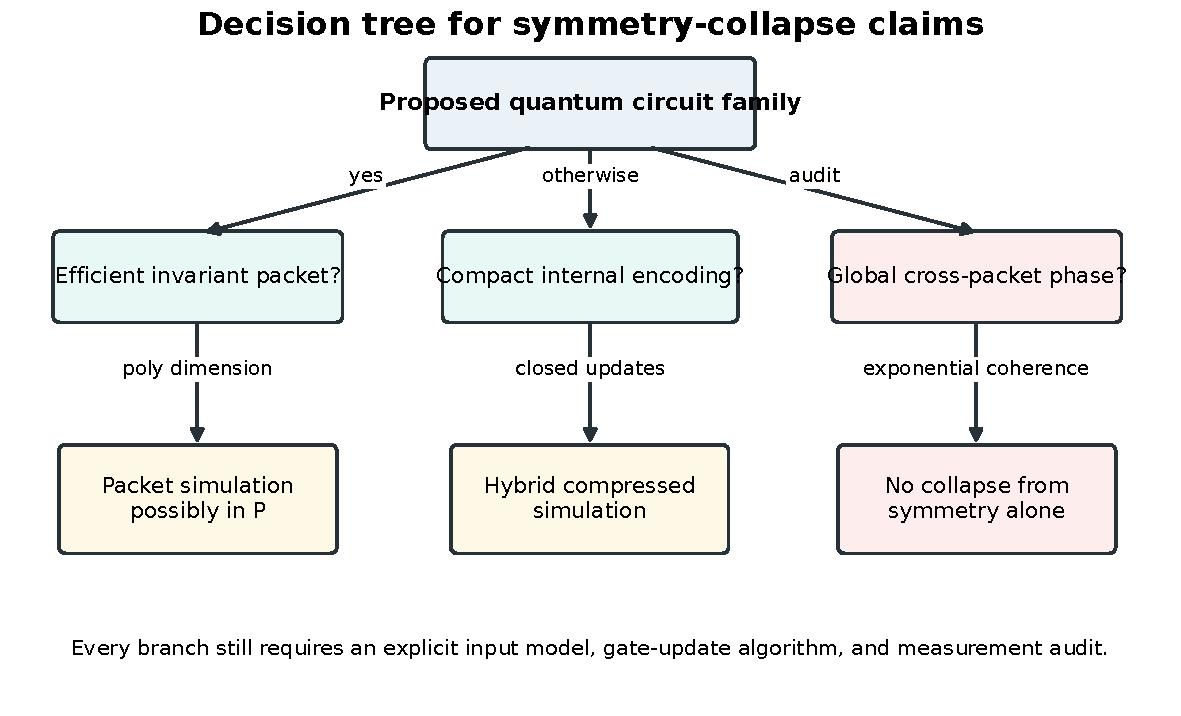
\includegraphics[width=.91\textwidth]{assets/s_collapse_decision_tree.pdf}
\caption{A disciplined decision tree for proposed symmetry-collapse claims.}
\end{figure}

\subsection{Why symmetry is only the beginning}
Suppose a group $G$ acts on the Hilbert space and the circuit commutes with this action. Representation theory decomposes the space into isotypic pieces. This gives a canonical block structure, but three questions remain.

First, how many pieces are reachable from the input? Second, how large is each piece or how compactly can its states be encoded? Third, can each gate and measurement be applied in those coordinates without reconstructing the full state? The monograph repeatedly returns to this three-stage distinction:
\[
\text{symmetry label}
\longrightarrow
\text{reachable representation}
\longrightarrow
\text{efficient classical algorithm}.
\]

\begin{principle}[No free collapse]
Block diagonality is a structural statement. Polynomial-time classical simulation requires an efficient basis or encoding, efficient updates, and efficient output evaluation in addition to the block decomposition.
\end{principle}

\section{Projectors and quantum packets}
\label{s:ch:projectors}
\index{projector}
\index{packet decomposition}

\subsection{Orthogonal packet decompositions}
Let $\Hh$ be a finite-dimensional Hilbert space and let $\{P_\alpha\}_{\alpha\in A}$ be orthogonal projectors satisfying
\[
P_\alpha P_\beta=\delta_{\alpha\beta}P_\alpha,
\qquad
\sum_{\alpha\in A}P_\alpha=I.
\]
Every state and operator decompose as
\[
\ket\psi=\sum_\alpha P_\alpha\ket\psi,
\qquad
X=\sum_{\alpha,\beta}P_\alpha X P_\beta.
\]
The diagonal blocks act within packets. The off-diagonal blocks transfer amplitude or coherence between packets.

Define the packet-transfer graph of an operator $X$ by placing an edge $\beta\to\alpha$ whenever
\[
P_\alpha X P_\beta\neq0.
\]
An exactly symmetry-preserving operator has only diagonal edges. A sparse transfer graph may still permit efficient simulation if the active packets and internal states remain compact.

\subsection{Conserved observables}
Let
\[
Q=\sum_k q_kP_k
\]
be a self-adjoint observable with spectral projectors $P_k$.

\begin{theorem}[Invariant quantum packets]
\label{s:thm:invariant-packets}
If a unitary $U$ satisfies $[U,Q]=0$, then
\[
P_iUP_j=0\qquad(i\neq j),
\]
and
\[
U=\bigoplus_i U_i,
\qquad
U_i=P_iUP_i\big|_{P_i\Hh}.
\]
If $P_k\ket\psi=\ket\psi$, then $P_kU\ket\psi=U\ket\psi$.
\end{theorem}

\begin{proof}
Since $U$ commutes with $Q$, it commutes with every spectral projector obtained from the functional calculus of $Q$. Thus
\[
P_iUP_j=UP_iP_j=0
\]
for $i\neq j$. Summing the diagonal blocks gives the direct-sum form. The final statement follows from
\[
P_kU\ket\psi=UP_k\ket\psi=U\ket\psi.
\]
\end{proof}

\subsection{Residue and character packets}
Suppose $Q$ has integer spectrum. For a modulus $M$, define
\[
B_r^{(M)}=
\sum_{k\equiv r\pmod M}P_k.
\]
Let
\[
V_M=\exp\left(\frac{2\pi i}{M}Q\right),
\qquad
\omega_M=e^{2\pi i/M}.
\]
Then
\begin{equation}
B_r^{(M)}
=
\frac1M\sum_{\ell=0}^{M-1}
\omega_M^{-r\ell}V_M^\ell.
\label{s:eq:residue-projector}
\end{equation}
On a $Q$-eigenvector, the right side is the roots-of-unity filter. The same finite-character formula selects residue classes in signal polyphase analysis and charge sectors in quantum theory.

\subsection{Finite-group projectors}
Let a finite group $G$ act unitarily by $U_g$. For an irreducible character $\chi$ of degree $d_\chi$, the central isotypic projector is
\begin{equation}
P_\chi
=
\frac{d_\chi}{|G|}
\sum_{g\in G}
\overline{\chi(g)}U_g.
\label{s:eq:character-projector}
\end{equation}
Character orthogonality gives
\[
P_\chi P_\psi=\delta_{\chi\psi}P_\chi,
\qquad
\sum_\chi P_\chi=I
\]
on the represented space. If an operator $A$ commutes with every $U_g$, then
\[
P_\chi A P_\psi=0
\qquad(\chi\neq\psi).
\]

This framework includes momentum, parity, total spin, point-group symmetry, permutation symmetry, and stabilizer syndrome labels. The isotypic projector identifies a symmetry type. It does not necessarily resolve the multiplicity space within that type.

\subsection{Nested refinements}
If one conserved label is too coarse, intersect commuting projector families. For mutually commuting observables $Q_1,\ldots,Q_s$, a joint packet has the form
\[
P_{\bm\alpha}
=
P^{(1)}_{\alpha_1}\cdots P^{(s)}_{\alpha_s}.
\]
The dimension can decrease dramatically, but each extra label must be efficiently computable and preserved. A refinement that requires exponential preprocessing merely relocates the complexity.

\begin{remark}
A packet decomposition is basis independent as an orthogonal direct sum, although a practical simulator must choose a concrete basis or compressed coordinate system within each active packet.
\end{remark}

\section{Uniform circuits and the classical cost model}
\label{s:ch:complexity-model}
\index{uniform circuit}
\index{classical simulation}

\subsection{Circuit families}
A quantum decision procedure is a polynomial-time uniform family of circuits $\{C_x\}$, where the input string $x$ determines a circuit on $n=n(|x|)$ qubits with at most $\poly(|x|)$ gates. Let
\[
C_x=G_m\cdots G_1.
\]
A classical simulation theorem must describe an algorithm receiving the same succinct description of $x$ and the circuit. It is not enough to assume that an exponentially large matrix or a complete orbit list has already been supplied.

\subsection{The packet access model}
For each input length, suppose there is a packet projector $P_n$ and a basis
\[
\B_n=
\{\ket{b_1},\ldots,\ket{b_{D_n}}\}
\]
of $P_n\Hh_n$. The simulation interface has four routines.

\begin{enumerate}
\item \textbf{Discovery and indexing.} Produce or index $\B_n$ in polynomial time.
\item \textbf{Initialization.} Express the initial state in this basis.
\item \textbf{Gate update.} Apply each restricted gate $P_nG_jP_n$ to the packet coordinates in polynomial time.
\item \textbf{Measurement.} Compute the final acceptance probability to the needed precision.
\end{enumerate}

The basis need not be listed explicitly if there is a compact data structure supporting these operations. Stabilizer tableaux and covariance matrices are examples of representations that encode exponentially many computational-basis amplitudes without storing them individually.

\subsection{Precision and promise gaps}
A BQP decision problem has an inverse-constant promise gap after standard amplification. A deterministic classical simulator need only estimate the acceptance probability to an additive error smaller than this gap. If the gate entries are algebraic or otherwise polynomial-time computable, ordinary numerical analysis gives polynomial bit complexity for polynomially many updates, provided condition numbers and error amplification are controlled.

\subsection{State-vector cost inside a packet}
If the simulator stores $D$ amplitudes and a local gate can be applied in $O(nD)$ arithmetic operations, a depth-$d$ packet simulation has schematic cost
\[
C_{\mathrm{packet}}=O(dnD)+C_{\mathrm{compile}}.
\]
The corresponding full state-vector path is
\[
C_{\mathrm{full}}=O(dn2^n).
\]
These formulas are intentionally schematic. Cache behavior, indexing, vectorization, and basis compilation determine actual runtime. The asymptotic distinction is exact when $D$ is polynomial and $2^n$ is exponential.

\subsection{Reuse and amortization}
Packet compilation can be expensive. Repeated parameter sweeps, time stepping, variational optimization, and repeated likelihood evaluation benefit from cached basis maps and gate plans. A one-shot simulation can be slower even when each subsequent packet update is much cheaper. The benchmark chapter preserves both one-shot and repeated-application measurements for this reason.

\begin{scopebox}
A polynomial-dimensional invariant sector does not guarantee a practical speedup at small $n$. It guarantees that the state-vector representation within that sector has polynomial asymptotic size under the stated access assumptions.
\end{scopebox}

\section{Exact packet simulation and polynomial collapse}
\label{s:ch:exact-simulation}

\subsection{Gatewise invariance}
Let $P$ be an orthogonal projector and suppose the initial state obeys $P\ket{\psi_0}=\ket{\psi_0}$. If every gate satisfies
\begin{equation}
G_jP=PG_jP,
\label{s:eq:gatewise-invariance}
\end{equation}
then $G_j$ maps $P\Hh$ into itself. For a general linear map, this equation asserts only invariance of the selected subspace. For the finite-dimensional unitary gates considered here, invariance also implies invariance of the orthogonal complement, so it is equivalent to commutation with $P$.

\begin{theorem}[Invariant-basis simulation]
\label{s:thm:invariant-basis}
Let $U=G_m\cdots G_1$ and assume \cref{s:eq:gatewise-invariance} for every gate. If $P\ket{\psi_0}=\ket{\psi_0}$, then
\[
U\ket{\psi_0}
=
(PG_mP)\cdots(PG_1P)\ket{\psi_0}.
\]
In any basis of $P\Hh$, the restricted circuit gives exactly the same amplitudes after embedding.
\end{theorem}

\begin{proof}
Inductively, if $P\ket{\psi_{j-1}}=\ket{\psi_{j-1}}$, then
\[
G_j\ket{\psi_{j-1}}
=
G_jP\ket{\psi_{j-1}}
=
PG_jP\ket{\psi_{j-1}},
\]
so the next state remains in $P\Hh$. Iterating proves the identity.
\end{proof}

\subsection{Polynomial packet-simulation theorem}
\begin{theorem}[Polynomial packet-simulation theorem]
\label{s:thm:poly-packet}
Let $\{C_x\}$ be a polynomial-time uniform family of quantum circuits. Suppose there is an efficiently computable packet representation such that:

\begin{enumerate}
\item the initial state lies in the represented packet and its coordinates are computable in polynomial time;
\item every gate preserves the representation;
\item the representation size is at most $\poly(|x|)$;
\item each gate update is computable to polynomial precision in polynomial time;
\item the final acceptance probability is computable from the representation in polynomial time.
\end{enumerate}

Then the language decided by the circuit family belongs to $P$.
\end{theorem}

\begin{proof}
The simulator stores a polynomial-size classical description of the evolving state. It performs polynomially many polynomial-time gate updates and evaluates the final measurement to inverse-polynomial precision. Choosing an error smaller than the amplified promise gap yields a deterministic polynomial-time decision algorithm.
\end{proof}

\begin{provedbox}
The theorem is a genuine quantum-to-classical complexity collapse for the declared subclass. It does not assume that a full $2^n$ state vector is ever constructed.
\end{provedbox}

\subsection{Dimension-only corollary}
A convenient special case uses an explicit basis of a packet of dimension $D_n$.

\begin{corollary}[Polynomial-dimensional invariant packet]
If $D_n\le\poly(n)$, the packet basis is efficiently indexed, every gate has a polynomial-time sparse or structured action in that basis, and the measurement is efficiently evaluable, then the circuit family is classically polynomial-time simulable.
\end{corollary}

\subsection{A broader compressed representation}
The state description need not be a vector of packet amplitudes. Let $\mathcal R_n$ be a polynomial-size classical representation class with an embedding into the packet Hilbert space. If initialization, gate updates, and measurement stay within $\mathcal R_n$ and are efficient, the same proof applies. This observation will later combine packet labels with stabilizer, Gaussian, or tensor-network coordinates.

\begin{figure}[H]
\centering
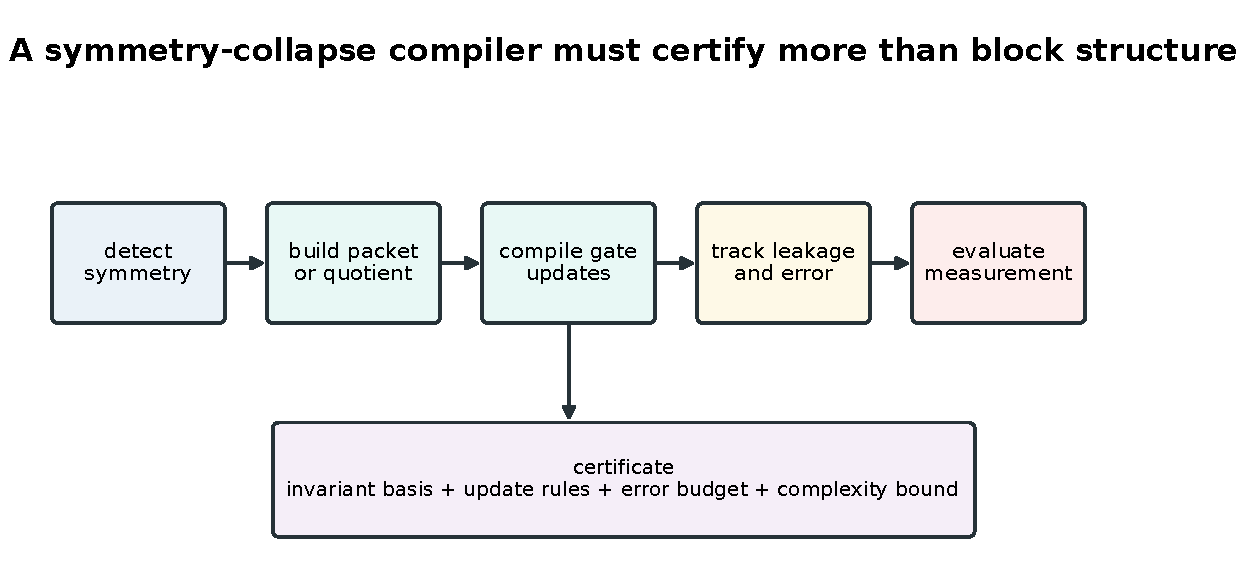
\includegraphics[width=.92\textwidth]{assets/s_compiler_pipeline.pdf}
\caption{A complete collapse certificate includes discovery, update, leakage, measurement, and complexity information.}
\end{figure}

\section{Approximate symmetry and leakage certificates}
\label{s:ch:approximate-symmetry}
\index{leakage}

\subsection{Hamiltonian leakage}
Exact conservation is not the only useful regime. Let $P$ be an orthogonal projector and let
\[
U(t)=e^{-itH}
\]
for a bounded self-adjoint Hamiltonian $H$. The leakage operator from the packet is
\[
L_P(t)=(I-P)e^{-itH}P.
\]

\begin{theorem}[Commutator leakage bound]
\label{s:thm:commutator-leakage}
For every real $t$,
\[
\|(I-P)e^{-itH}P\|
\le
|t|\,\|[H,P]\|.
\]
\end{theorem}

\begin{proof}
Define
\[
F(s)=e^{-i(t-s)H}Pe^{-isH}P.
\]
Then $F(0)=e^{-itH}P$ and $F(t)=Pe^{-itH}P$. Differentiation gives
\[
F'(s)=ie^{-i(t-s)H}[H,P]e^{-isH}P.
\]
Therefore
\[
(I-P)e^{-itH}P
=-(I-P)\int_0^tF'(s)\,ds.
\]
The unitary factors and projectors have norm at most one, so the integral is bounded by $|t|\|[H,P]\|$.
\end{proof}

\subsection{Circuit leakage}
For a gate $G_j$, define
\[
\delta_j=\|(I-P)G_jP\|.
\]
Let $V_j=PG_jP$. A telescoping expansion gives
\[
G_m\cdots G_1P-V_m\cdots V_1P
=
\sum_{k=1}^m
G_m\cdots G_{k+1}(G_k-V_k)V_{k-1}\cdots V_1P.
\]
Taking norms yields the following.

\begin{proposition}[Sum-of-leakages bound]
\label{s:prop:sum-leakage}
For an initial state in $P\Hh$,
\[
\|G_m\cdots G_1\ket{\psi_0}
-
V_m\cdots V_1\ket{\psi_0}\|
\le
\sum_{j=1}^m\delta_j.
\]
\end{proposition}

This is conservative because leakage contributions may interfere destructively. Its value is that it is composable and can be checked gate by gate.

\subsection{Decision-problem consequence}
If the packet representation is polynomial, the restricted updates are efficient, and
\[
\sum_j\delta_j\le\frac1{\poly(n)},
\]
then the approximate packet simulator reproduces the final acceptance probability to inverse-polynomial accuracy. After ordinary promise-gap amplification, this suffices for a deterministic polynomial-time decision algorithm.

\subsection{Adaptive packet enlargement}
A practical simulator need not fix one packet forever. It can maintain an active set $A_t$ of packets, estimate transfers $P_\alpha G_tP_\beta$, and add a packet when its predicted mass exceeds a tolerance. The proof obligation becomes a global accounting identity:
\[
\text{total error}
\le
\text{discarded transfer}
+
\text{numerical error}
+
\text{measurement approximation}.
\]
The key research problem is to retain polynomial active size while certifying the tail.

\begin{figure}[H]
\centering
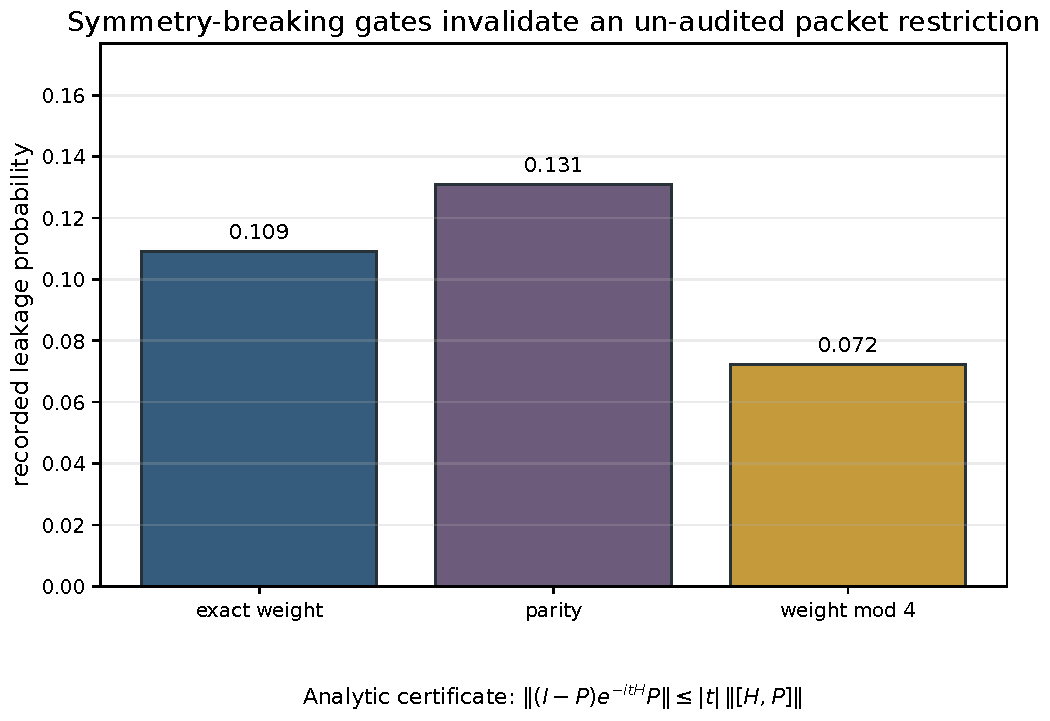
\includegraphics[width=.76\textwidth]{assets/s_leakage_bound.pdf}
\caption{Recorded leakage examples and the analytic commutator certificate.}
\end{figure}

\section{Moving packets, dynamic frames, and sparse transfer graphs}
\label{s:ch:dynamic-frames}
\index{moving packet}
\index{time-dependent projector}
\index{packet transfer graph}

\subsection{Why one fixed projector is not the end of the theory}
The exact packet theorem in \cref{s:ch:exact-simulation} follows a state inside one fixed subspace. That is sufficient for a conserved charge, but it is not necessary for classical collapse. A circuit may move through a sequence of small subspaces, or it may preserve a small packet only after a time-dependent change of coordinates. The correct object is therefore a \emph{packet schedule}, not necessarily one static projector.

\begin{definition}[Packet schedule]
For a circuit
\[
U=G_m\cdots G_1
\]
on a Hilbert space $\Hh$, a packet schedule is a sequence of orthogonal projectors
\[
P_0,P_1,\ldots,P_m.
\]
It is exact when
\begin{equation}
G_tP_{t-1}=P_tG_tP_{t-1}
\qquad(1\le t\le m).
\label{s:eq:dynamic-packet-condition}
\end{equation}
\end{definition}

The condition says that gate $G_t$ maps the currently active packet into the next active packet. The dimensions may vary with time.

\subsection{Exact dynamic-packet simulation}
Choose isometries
\[
B_t:\C^{D_t}\longrightarrow\Hh,
\qquad
B_tB_t^*=P_t,
\qquad
B_t^*B_t=I_{D_t},
\]
where $D_t=\rank P_t$. Define the rectangular coordinate update
\begin{equation}
M_t=B_t^*G_tB_{t-1}.
\label{s:eq:dynamic-coordinate-update}
\end{equation}

\begin{theorem}[Exact dynamic-packet theorem]
\label{s:thm:dynamic-packet}
Suppose $P_0\ket{\psi_0}=\ket{\psi_0}$ and \cref{s:eq:dynamic-packet-condition} holds for every gate. Put
\[
z_0=B_0^*\ket{\psi_0},
\qquad
z_t=M_tz_{t-1}.
\]
Then
\[
G_t\cdots G_1\ket{\psi_0}=B_tz_t
\]
for every $t$.
\end{theorem}

\begin{proof}
The claim is true at $t=0$. If the state after $t-1$ gates is $B_{t-1}z_{t-1}$, then
\[
G_tB_{t-1}z_{t-1}
=P_tG_tP_{t-1}B_{t-1}z_{t-1}
=B_tB_t^*G_tB_{t-1}z_{t-1}
=B_tM_tz_{t-1}.
\]
This is $B_tz_t$.
\end{proof}

\begin{theorem}[Polynomial moving-packet collapse]
\label{s:thm:moving-packet-collapse}
Let $\{C_x\}$ be a polynomial-time uniform circuit family. Suppose an exact packet schedule can be produced from $x$ in polynomial time such that:
\begin{enumerate}
\item $\max_tD_t\le\poly(|x|)$;
\item the coordinate description of the initial state is computable in polynomial time;
\item each rectangular update $M_t$ can be applied to polynomial precision in polynomial time;
\item the final acceptance probability is computable from $z_m$ in polynomial time.
\end{enumerate}
Then the language decided by the circuit family belongs to $P$.
\end{theorem}

\begin{proof}
The simulator stores at most polynomially many coordinates at every step and applies polynomially many polynomial-time updates. \Cref{s:thm:dynamic-packet} proves exactness before numerical rounding. Polynomial precision below the amplified promise gap gives a deterministic polynomial-time decision procedure.
\end{proof}

\begin{derivedbox}
A circuit does not need one globally conserved sector. It is enough that the state follow an efficiently discoverable path through polynomial-dimensional sectors.
\end{derivedbox}

\subsection{Moving frames and hidden symmetry}
The packet schedule has a useful coordinate form. Let $P$ be one fixed projector and let $W_t$ be unitaries with
\[
P_t=W_tPW_t^*.
\]
In the moving frame, the transformed gate is
\begin{equation}
\widetilde G_t
=W_t^*G_tW_{t-1}.
\label{s:eq:moving-frame-gate}
\end{equation}
The schedule condition is equivalent to
\[
\widetilde G_tP=P\widetilde G_tP.
\]

\begin{corollary}[Moving-frame collapse]
\label{s:cor:moving-frame-collapse}
Suppose a polynomial-time uniform circuit admits efficiently described frames $W_t$ for which the transformed gates in \cref{s:eq:moving-frame-gate} preserve one fixed polynomial-dimensional packet, the initial state has efficiently computable coordinates in $W_0P\Hh$, and their restricted matrices and the transformed final measurement are efficiently computable. Then the circuit family is classically simulable in polynomial time.
\end{corollary}

This is the appropriate theorem for a symmetry that changes orientation with time. Examples to test include Clifford frames, Gaussian mode frames, rotating spin axes, and gauge-fixed local coordinates.

\begin{scopebox}
The frame must be independently discoverable and efficiently usable. Choosing $W_t=G_t\cdots G_1$ makes the transformed state trivial but is circular: computing that frame is the original simulation problem. The theorem is useful only when the frames have a compact classical description and their restricted actions can be computed without constructing the full state.
\end{scopebox}

\begin{figure}[H]
\centering
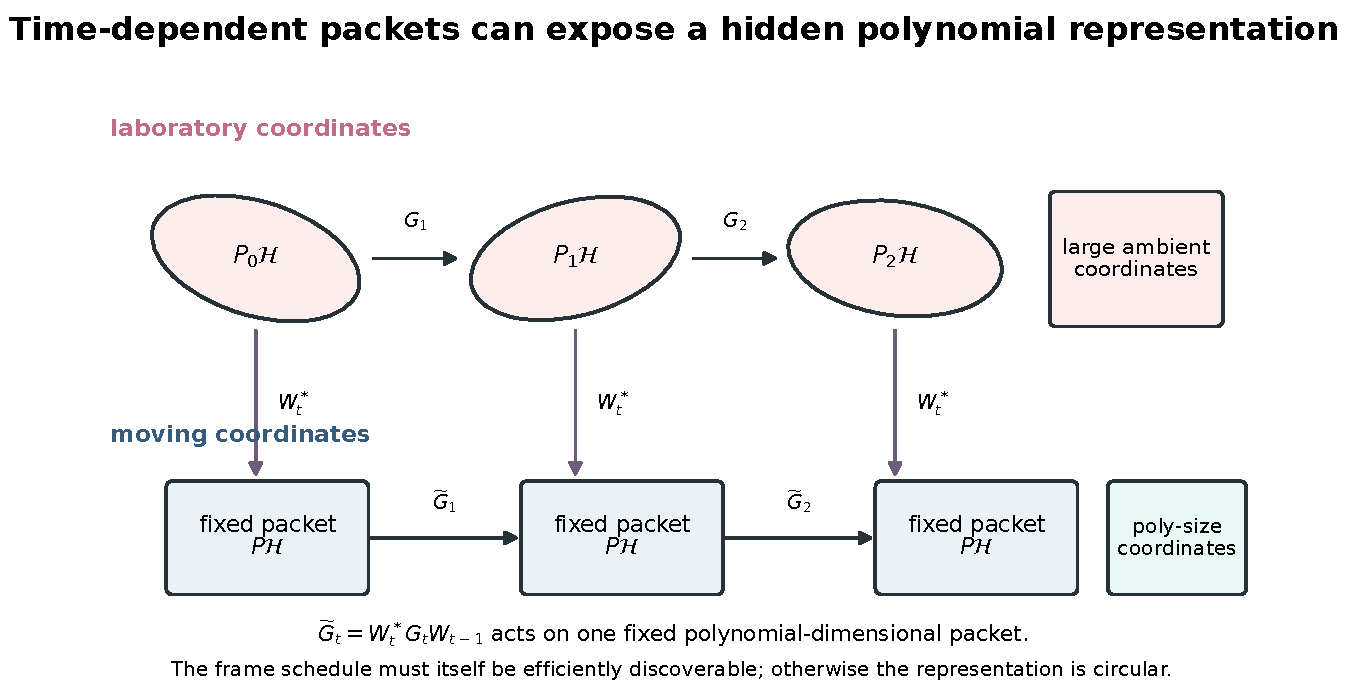
\includegraphics[width=.94\textwidth]{assets/s_moving_frame_packets.pdf}
\caption{A circuit may fail to preserve one laboratory-frame packet while remaining inside a small packet in a computable moving frame.}
\end{figure}

\subsection{Sparse packet-transfer graphs}
Let
\[
I=\sum_{\alpha\in\Lambda}P_\alpha
\]
be an orthogonal packet decomposition. Write the gate blocks as
\[
G_{t;\beta\alpha}=P_\beta G_tP_\alpha.
\]
Starting from an active packet set $S_0$, define recursively
\begin{equation}
S_t
=
\left\{
\beta:\exists\alpha\in S_{t-1}
\text{ with }G_{t;\beta\alpha}\ne0
\right\}.
\label{s:eq:reachable-packet-set}
\end{equation}

\begin{corollary}[Reachable packet-graph collapse]
\label{s:cor:packet-graph-collapse}
Suppose the packet sets $S_t$ and nonzero transfer blocks are computable in polynomial time, and
\[
D_t
=
\sum_{\alpha\in S_t}\rank P_\alpha
\le\poly(n)
\]
for every $t$. If all active block updates and the final measurement are efficiently computable, then the circuit family is classically polynomial-time simulable.
\end{corollary}

\begin{proof}
Take
\[
P_t=\sum_{\alpha\in S_t}P_\alpha.
\]
The definition of $S_t$ gives $G_tP_{t-1}=P_tG_tP_{t-1}$. Apply \cref{s:thm:moving-packet-collapse}.
\end{proof}

This theorem permits exact sector changes. What matters is not that one charge be fixed, but that the union of reachable sectors remain polynomial.

\begin{corollary}[Bounded-excitation collapse]
\label{s:cor:bounded-excitation-collapse}
Consider $n$ qubits and suppose the initial state and every circuit prefix are certified to lie in
\[
\Hh_{\le K}
=
\bigoplus_{k=0}^{K}\Hh_{n,k}
\]
for a fixed constant $K$. If initialization, the gate actions, and the measurement are computable in polynomial time in the occupation basis, then the circuit family lies in $P$, even when individual gates change excitation number.
\end{corollary}

\begin{proof}
The active dimension is
\[
\sum_{k=0}^{K}\binom nk
=O(n^K).
\]
Let $P$ project onto $\Hh_{\le K}$. By the hypothesis on the actual circuit prefixes, $P\psi_t=\psi_t$ at every step. Consequently $PG_tP\psi_{t-1}=G_t\psi_{t-1}$ on the evolving state, even if the gate does not preserve all of $P\Hh$. The restricted update therefore reproduces that trajectory exactly. The hypothesis supplies efficient initialization, updates, and measurement in these polynomially many coordinates.
\end{proof}

For example, a fixed-weight input followed by only a constant number of pair-creation or pair-annihilation events remains in a constant collection of low-weight sectors. Exact number conservation is therefore stronger than necessary.

\begin{figure}[H]
\centering
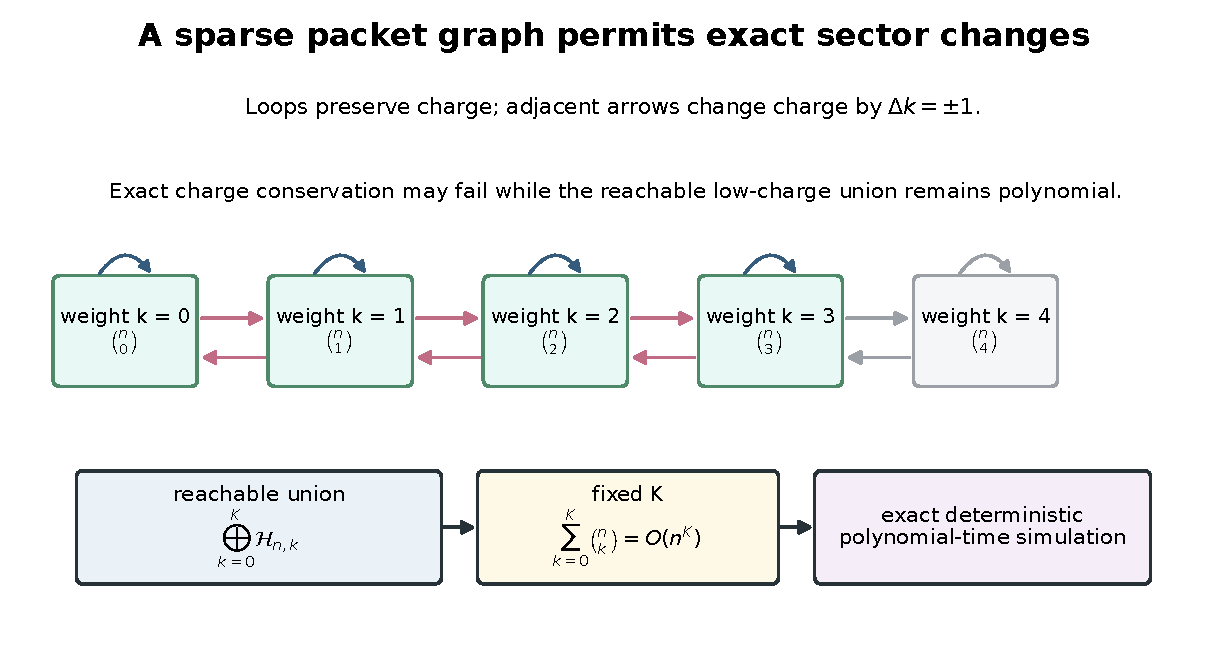
\includegraphics[width=.90\textwidth]{assets/s_reachable_packet_graph.pdf}
\caption{Sector-changing gates remain classically tractable when the reachable packet graph and total active dimension stay polynomial.}
\end{figure}

\subsection{Approximate dynamic packets}
Define the one-step leakage from the scheduled packet by
\[
\delta_t
=
\|(I-P_t)G_tP_{t-1}\|.
\]
Let
\[
\widehat G_t=P_tG_tP_{t-1}.
\]

\begin{theorem}[Dynamic sum-of-leakages bound]
\label{s:thm:dynamic-leakage}
For an initial unit vector in $P_0\Hh$,
\[
\left\|
G_m\cdots G_1\ket{\psi_0}
-
\widehat G_m\cdots\widehat G_1\ket{\psi_0}
\right\|
\le
\sum_{t=1}^{m}\delta_t.
\]
For any acceptance operator $0\le M\le I$, the corresponding acceptance probabilities differ by at most
\[
2\sum_{t=1}^{m}\delta_t.
\]
\end{theorem}

\begin{proof}
A telescoping expansion inserts $G_t-\widehat G_t$ at one time. On $P_{t-1}\Hh$ this difference equals $(I-P_t)G_tP_{t-1}$, while all other unitary or projected factors have norm at most one. Summing the operator norms proves the state bound. If $\psi$ and $\phi$ have norm at most one, then
\[
|\langle\psi,M\psi\rangle-\langle\phi,M\phi\rangle|
\le
(\|\psi\|+\|\phi\|)\|\psi-\phi\|
\le2\|\psi-\phi\|.
\]
\end{proof}

\begin{corollary}[Approximate moving-packet collapse]
If the scheduled dimensions and updates are polynomial and
\[
\sum_t\delta_t\le\frac1{\poly(n)},
\]
then, after ordinary promise-gap amplification, the circuit family remains deterministically classically simulable in polynomial time.
\end{corollary}

The result is conservative but fully composable. It extends the fixed-projector estimate of \cref{s:ch:approximate-symmetry} to moving frames and changing packet sets.


\subsection{An adaptive certificate from discarded state vectors}
The operator-norm leakage certificate is uniform over every input in a packet. An adaptive simulator can use a less expensive certificate that follows its actual approximate state. The discarded vector must be accounted for before any normalization.

\begin{theorem}[Adaptive discarded-state certificate]
\label{s:thm:adaptive-discarded-state}
Let $G_1,\ldots,G_m$ be unitary operators on a finite-dimensional Hilbert space, and let $\psi_0=\phi_0$ be a unit vector. At each step choose an orthogonal projector $P_t$, possibly as a function of the previously computed approximate states. Define
\[
\psi_t=G_t\psi_{t-1},\qquad
\phi_t=P_tG_t\phi_{t-1},\qquad
\eta_t=\|(I-P_t)G_t\phi_{t-1}\|.
\]
Then
\[
\|\psi_m-\phi_m\|\le\sum_{t=1}^m\eta_t.
\]
For an effect $0\le M\le I$,
\[
\left|\langle\psi_m,M\psi_m\rangle-\langle\phi_m,M\phi_m\rangle\right|
\le2\sum_{t=1}^m\eta_t.
\]
No renormalization of $\phi_t$ is performed. The second quadratic form is an unnormalized acceptance estimate.
\end{theorem}

\begin{proof}
Fix the projectors chosen during the particular run. Put $d_t=(I-P_t)G_t\phi_{t-1}$. Subtraction gives the exact recurrence
\[
\psi_t-\phi_t=G_t(\psi_{t-1}-\phi_{t-1})+d_t.
\]
Since $\psi_0-\phi_0=0$, iteration yields
\[
\psi_m-\phi_m=\sum_{t=1}^mG_m\cdots G_{t+1}d_t.
\]
Every unitary product preserves norm, so the triangle inequality proves the state estimate. Also $\|\psi_m\|=1$ and $\|\phi_m\|\le1$ because each projector is contractive. Expanding the difference of the two quadratic forms and using $\|M\|\le1$ gives the factor two. This proof applies to the chosen run even when the projectors were selected adaptively.
\end{proof}

\begin{example}[A rational two-step certificate]
Take
\[
G=\begin{pmatrix}3/5&-4/5\\4/5&3/5\end{pmatrix},
\qquad
P=\begin{pmatrix}1&0\\0&0\end{pmatrix},
\qquad
\psi_0=\phi_0=\begin{pmatrix}1\\0\end{pmatrix}.
\]
Using $G_1=G_2=G$ and $P_1=P_2=P$ gives
\[
\phi_2=\begin{pmatrix}9/25\\0\end{pmatrix},\qquad
\psi_2=\begin{pmatrix}-7/25\\24/25\end{pmatrix},\qquad
\eta_1=4/5,\quad\eta_2=12/25.
\]
The squared state error is $832/625$, below $(\eta_1+\eta_2)^2=1024/625$. The rational validation script checks these values exactly. The deliberately large tail illustrates a valid but loose certificate, not an efficient approximation.
\end{example}

The theorem closes global error accounting for any adaptive projection run whose discarded vectors or certified norm bounds can be computed. It does not prove that the retained representation stays polynomial, that the discarded norm is cheap to evaluate, or that a small tail can always be found. Those are separate algorithmic obligations. This is a written theorem with exact finite controls, not an additional Lean formalization.

\chapter{Exact symmetry families}
\section{Fixed charge and exact-number circuits}
\label{s:ch:fixed-charge}
\index{Hamming weight}
\index{particle number}

\subsection{Excitation-number packets}
For $n$ qubits, define
\[
\widehat N
=
\sum_{q=1}^n\frac{I-Z_q}{2}.
\]
Its eigenvalues are $k=0,1,\ldots,n$. The projector onto Hamming weight $k$ is
\[
P_{n,k}
=
\sum_{|x|=k}\ket x\bra x,
\]
and
\[
\dim P_{n,k}\Hh
=
\binom nk.
\]
The decomposition
\[
(\C^2)^{\otimes n}
=
\bigoplus_{k=0}^n\Hh_{n,k}
\]
recovers the full dimension through
\[
\sum_{k=0}^n\binom nk=2^n.
\]

\subsection{Number-preserving gates}
Single-qubit $R_Z$ gates commute with $\widehat N$. A two-qubit exchange rotation acts in the ordered basis $\ket{00},\ket{01},\ket{10},\ket{11}$ as
\[
U_{XY}(\theta,\phi)
=
\begin{pmatrix}
1&0&0&0\\
0&\cos\theta&-ie^{-i\phi}\sin\theta&0\\
0&-ie^{i\phi}\sin\theta&\cos\theta&0\\
0&0&0&1
\end{pmatrix}.
\]
It rotates $\ket{01}$ and $\ket{10}$ while fixing $\ket{00}$ and $\ket{11}$, so it preserves exact Hamming weight.

\begin{corollary}[Fixed-charge polynomial simulation]
\label{s:cor:fixed-charge-poly}
For every fixed $k$, a polynomial-time uniform family of number-preserving circuits initialized in $\Hh_{n,k}$ and measured by an efficiently computable observable is classically simulable in polynomial time, provided the initial weight-$k$ coordinates can be computed efficiently and each restricted local gate is efficiently applied in that basis.
\end{corollary}

\begin{proof}
For fixed $k$,
\[
\dim\Hh_{n,k}=\binom nk=O(n^k).
\]
The weight-$k$ basis is efficiently indexed by $k$-element subsets. A local number-preserving gate changes only basis states containing the affected occupation pattern. Apply \cref{s:thm:poly-packet}.
\end{proof}

\subsection{Sparse update structure}
A one-qubit diagonal phase changes one amplitude at a time. An exchange gate on modes $p,q$ couples a basis state only to the state obtained by moving one excitation between those modes. Thus every column of the restricted gate has at most two nonzero entries. For fixed $k$, the total update cost is polynomial in $n$.

\subsection{Uniformity and input encoding}
The fixed-charge corollary assumes $k$ is a fixed constant independent of $n$. It also applies when $k=O(1)$ is supplied by the circuit family. If $k$ is written in binary and allowed to scale as $n/2$, the sector can become exponential. The theorem is about the dimension and update cost of the actual active sector, not the name of the symmetry.

\begin{figure}[H]
\centering
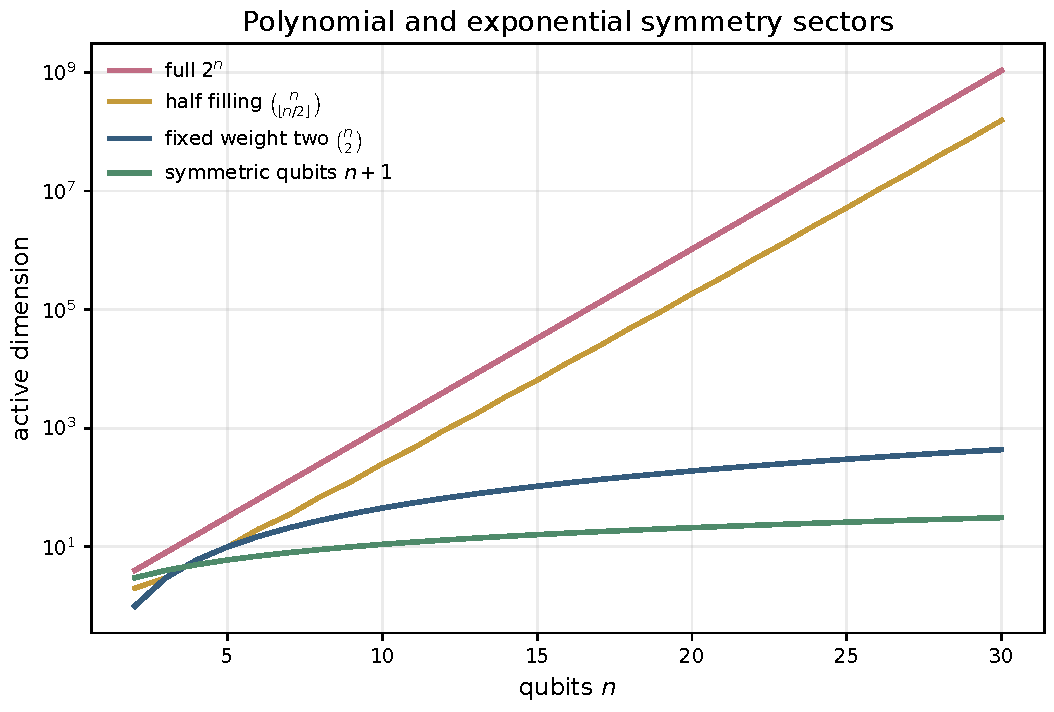
\includegraphics[width=.83\textwidth]{assets/s_dimension_scaling.pdf}
\caption{Fixed weight and permutation symmetry can be polynomial, while half filling remains exponential.}
\end{figure}

\subsection{Observables}
A diagonal observable depending on occupations is immediate. Few-body number-preserving observables are sparse in the subset basis. More global observables may require additional structure. The measurement hypothesis in \cref{s:thm:poly-packet} cannot be omitted: a compactly evolved state does not help if the requested output itself hides exponential work.

\section{The exact weight-two benchmark}
\label{s:ch:benchmarks}
\index{benchmark}

\subsection{Purpose and status}
The benchmark record compares a full state-vector simulator with a simulator restricted to the exact weight-two packet. Both use the same local gate arithmetic. The benchmark is not a hardware claim and not a universal performance model. It shows that the exact dimension reduction can translate into large memory and repeated-application gains in an ordinary implementation.

\begin{recordbox}
At $n=20$, the full state has $1{,}048{,}576$ amplitudes and the exact weight-two packet has $190$. The archived repeated-application gain is $958.8$, the one-shot gain is $54.8$, and the amplitude-memory ratio is $5518.8$. The recorded relative reconstruction error is zero at the displayed precision.
\end{recordbox}

\subsection{Recorded table}
\begin{longtable}{@{}rrrrrrr@{}}
\caption{Recorded exact-weight-two benchmark.}\label{s:tab:weight-two}\\
\toprule
$n$ & full dim. & packet dim. & apply gain & one-shot gain & memory gain & rel. error\\
\midrule
\endfirsthead
\toprule
$n$ & full dim. & packet dim. & apply gain & one-shot gain & memory gain & rel. error\\
\midrule
\endhead
8 & 256 & 28 & 1.11 & 1.64 & 9.14 & 0\\
10 & 1,024 & 45 & 1.51 & 2.02 & 22.8 & 0\\
12 & 4,096 & 66 & 2.95 & 3.98 & 62.1 & 0\\
14 & 16,384 & 91 & 8.55 & 11.0 & 180.0 & 0\\
16 & 65,536 & 120 & 33.0 & 36.9 & 546.1 & 0\\
18 & 262,144 & 153 & 131.3 & 39.1 & 1,713.4 & 0\\
20 & 1,048,576 & 190 & 958.8 & 54.8 & 5,518.8 & 0\\
\bottomrule
\end{longtable}

\subsection{What is machine independent}
The dimension identity
\[
\frac{2^n}{\binom n2}
\]
is independent of implementation. It predicts an exponential memory advantage for fixed $k=2$. The measured runtime ratio need not equal the dimension ratio. Packet indexing, compilation, sparse update kernels, allocation, and cache behavior determine the constant factors.

\subsection{Repeated application versus one shot}
Let $C_{\rm compile}$ be the cost of constructing the packet basis and restricted gate plans, and let $C_{\rm apply}$ be one packet application. Reusing the compiled plan $R$ times costs
\[
C_{\rm packet}(R)
=
C_{\rm compile}+RC_{\rm apply}.
\]
If the full path costs $RC_{\rm full}$, the packet method breaks even when
\[
R>
\frac{C_{\rm compile}}
{C_{\rm full}-C_{\rm apply}}.
\]
This is why time evolution, parameter sweeps, variational loops, and repeated likelihood evaluations are natural applications.

\begin{figure}[H]
\centering
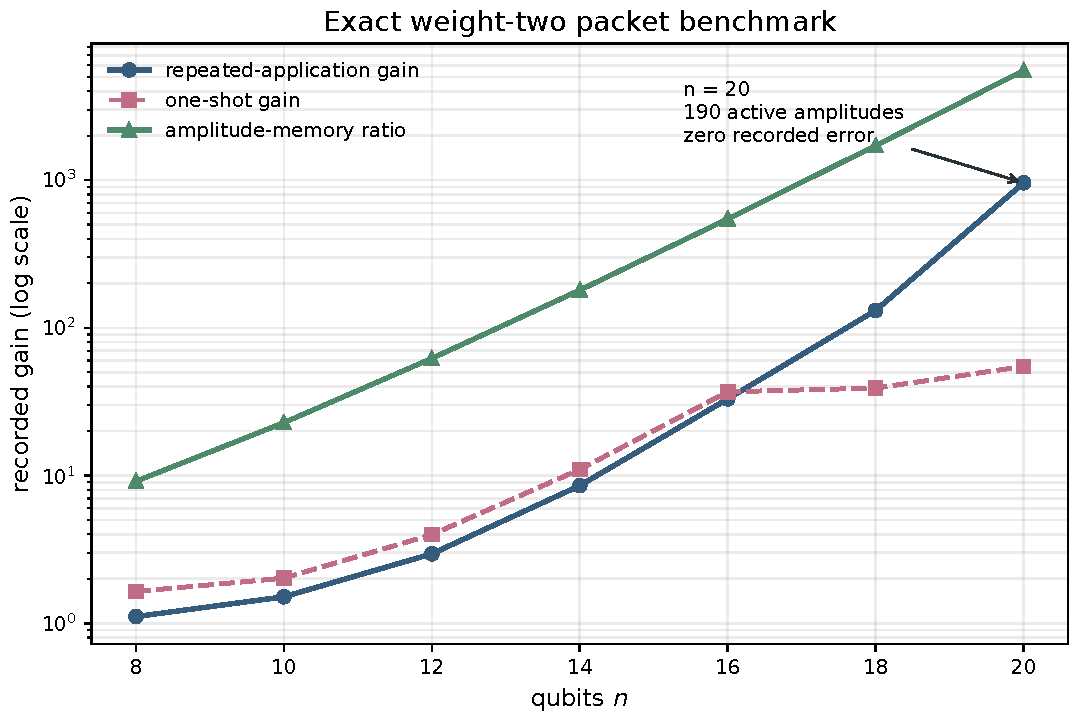
\includegraphics[width=.86\textwidth]{assets/s_weight_two_benchmark.pdf}
\caption{Recorded runtime and memory gains for the exact-weight-two packet.}
\end{figure}

\subsection{Independent reconstruction check}
The release code generates a random packet state, embeds it in the full Hilbert space, applies the same $R_Z$ and exchange gates through both arithmetic paths, and compares the final states. The representative checks at $(n,k)=(6,1),(8,2),(10,2)$ produce errors near machine precision.

\paragraph{Scope.}
The recorded benchmark supports exactness and implementation value for a symmetry-preserving subclass. It does not show that generic quantum circuits admit comparable reductions.

\section{Coarse packets and the honest limitation}
\label{s:ch:coarse-packets}

\subsection{Parity}
The even- and odd-parity packets each have dimension
\[
2^{n-1}.
\]
Parity removes half the state vector. This can produce a useful constant factor, but it does not change exponential scaling.

A pair-creation rotation mixes $\ket{00}$ and $\ket{11}$ and therefore changes excitation number by two while preserving parity. The packet is exact for a parity-preserving circuit, but its internal dimension remains exponential.

\subsection{Weight modulo four}
A four-qubit rotation between $\ket{0000}$ and $\ket{1111}$ changes excitation number by four. It can mix exact-weight sectors while preserving weight modulo four. A single residue packet contains asymptotically one quarter of all basis states. Again, the reduction is a constant factor.

\subsection{Half filling}
At half filling,
\[
\binom n{\lfloor n/2\rfloor}
\sim
\frac{2^n}{\sqrt{\pi n/2}}.
\]
The packet is smaller by a polynomial factor, but it remains exponential. At $n=20$, the half-filled packet contains $184{,}756$ amplitudes. The archived repeated-application gain is approximately $7.396$, while the one-shot gain is $0.6529$, meaning the packet path was slower in that single-run test after compilation overhead.

\begin{recordbox}
The half-filled benchmark demonstrates a necessary distinction: dimension reduction can be exact and useful without yielding polynomial complexity or a one-shot speedup.
\end{recordbox}

\begin{figure}[H]
\centering
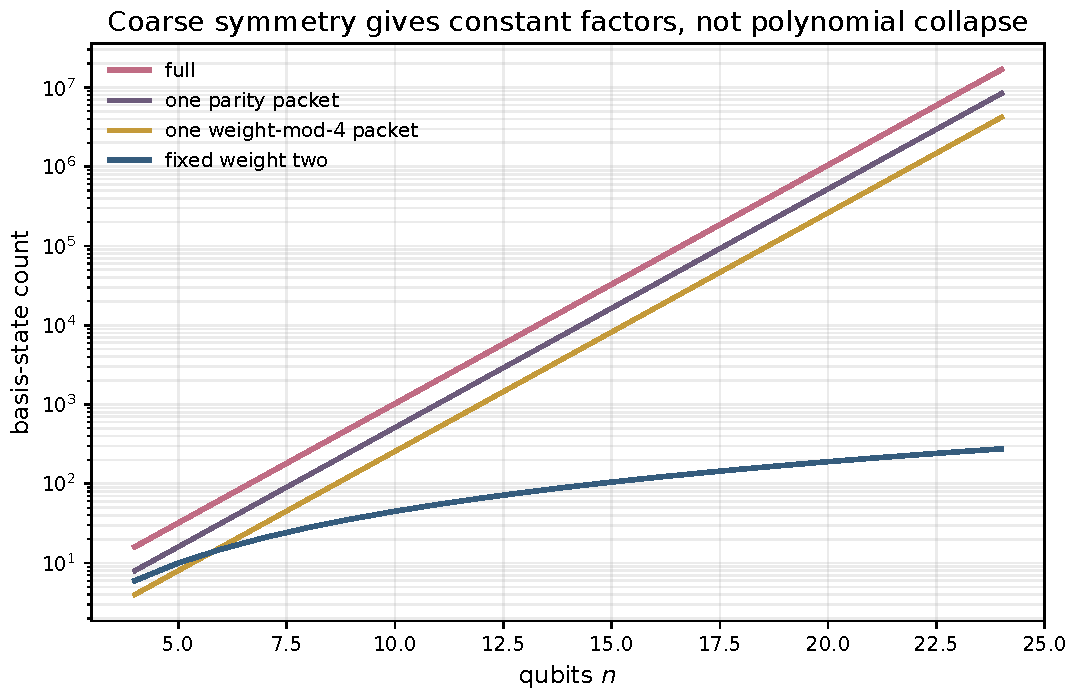
\includegraphics[width=.82\textwidth]{assets/s_coarse_vs_fine.pdf}
\caption{Parity and mod-four packets retain an exponential number of basis states.}
\end{figure}

\subsection{Entanglement inside a packet}
A small number of symmetry labels does not imply low entanglement. The half-filled packet can support volume-law entanglement. Tensor-network bond dimension and packet dimension are independent resources. A robust simulator should therefore track both
\[
(D_{\rm packet},\chi_{\rm internal}),
\]
where $\chi_{\rm internal}$ measures the cost of representing the state inside the packet.

\subsection{The no-label shortcut}
A stabilizer syndrome is only a label. A momentum quantum number is only a label. A total charge residue is only a label. The internal multiplicity space may still contain exponentially many degrees of freedom. The packet-simulation theorem becomes polynomial only when the complete active representation, not merely the label set, has polynomial classical cost.

\section{Permutation-symmetric circuits and Dicke coordinates}
\label{s:ch:permutation-symmetry}
\index{Dicke state}
\index{permutation symmetry}

\subsection{The symmetric subspace}
Let the symmetric group $S_n$ act by permuting the $n$ tensor factors. The fully symmetric qubit subspace is spanned by the Dicke states
\[
\ket{D_n^k}
=
\binom nk^{-1/2}
\sum_{|x|=k}\ket x,
\qquad
0\le k\le n.
\]
Its dimension is $n+1$.

\begin{derivedbox}
If the initial state is permutation symmetric with efficiently computable Dicke coordinates, every gate preserves the fully symmetric subspace, the gate matrices in the Dicke basis are computable in polynomial time, and the final measurement is permutation invariant and efficient, then the circuit family lies in $P$.
\end{derivedbox}

\begin{theorem}[Permutation-symmetric collapse]
\label{s:thm:permutation-collapse}
Under the hypotheses above, an $n$-qubit circuit can be simulated using an $(n+1)$-component classical state vector and polynomial-time updates.
\end{theorem}

\begin{proof}
The projector onto the trivial $S_n$ representation has rank $n+1$. The Dicke basis is explicitly indexed by $k=0,\ldots,n$. Apply \cref{s:thm:poly-packet}.
\end{proof}

\begin{figure}[H]
\centering
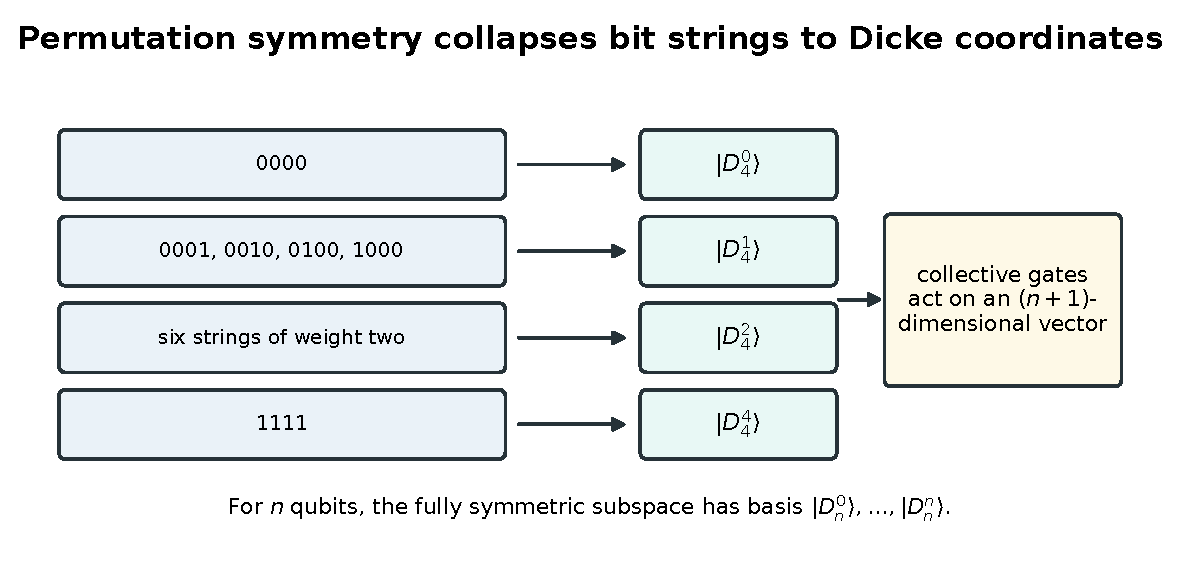
\includegraphics[width=.94\textwidth]{assets/s_dicke_basis.pdf}
\caption{Computational-basis orbits become Dicke coordinates.}
\end{figure}

\subsection{Collective spin operators}
Define
\[
J_a=\frac12\sum_{q=1}^n\sigma_a^{(q)},
\qquad a\in\{x,y,z\}.
\]
The operators $J_a$ preserve the symmetric subspace. We use the computational convention $\sigma_z\ket0=\ket0$ and $\sigma_z\ket1=-\ket1$. Thus $J_z\ket{D_n^k}=(n/2-k)\ket{D_n^k}$. For the following occupation formulas define $J_+=J_x-iJ_y$ and $J_-=J_x+iJ_y$, so that the subscript records increasing or decreasing excitation number rather than magnetic quantum number. Then
\[
J_+\ket{D_n^k}
=
\sqrt{(n-k)(k+1)}\ket{D_n^{k+1}},
\]
\[
J_-\ket{D_n^k}
=
\sqrt{k(n-k+1)}\ket{D_n^{k-1}}.
\]
Thus collective rotations and polynomial functions of collective spin admit banded or structured updates on $n+1$ amplitudes.

\subsection{Symmetric qudits}
For local dimension $d$, the symmetric subspace has occupation-number basis
\[
(n_1,\ldots,n_d),
\qquad
n_1+\cdots+n_d=n,
\]
and dimension
\begin{equation}
\dim\Sym^n(\C^d)
=
\binom{n+d-1}{d-1}.
\label{s:eq:symmetric-qudit-dim}
\end{equation}
For fixed $d$, this is polynomial in $n$.

\begin{corollary}[Fixed-local-dimension symmetric qudits]
A uniform family of fully symmetric $d$-level circuits is classically polynomial-time simulable for fixed $d$, provided its occupation-basis updates and measurement are polynomial-time computable.
\end{corollary}

\begin{figure}[H]
\centering
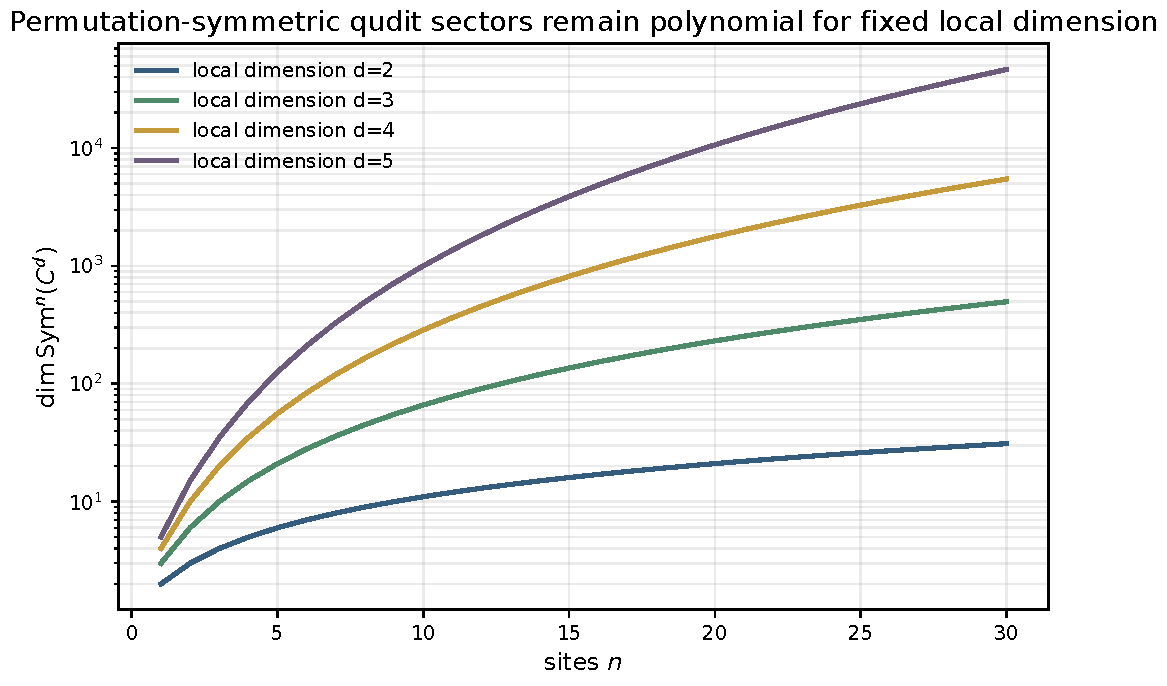
\includegraphics[width=.80\textwidth]{assets/s_symmetric_qudit_scaling.pdf}
\caption{Symmetric qudit sectors remain polynomial for every fixed local dimension.}
\end{figure}

\subsection{What full symmetry excludes}
A generic two-qubit gate acting on one selected pair does not preserve the fully symmetric subspace. Symmetry is preserved by collective gates or by circuits arranged so that the total operation commutes with all permutations. A gatewise packet simulator requires gatewise invariance, or else it must combine several elementary gates into a symmetry-preserving layer and audit intermediate leakage.

\section{Schur--Weyl coordinates and total-spin packets}
\label{s:ch:schur}
\index{Schur-Weyl duality}

\subsection{Decomposition}
For $n$ qudits of local dimension $d$, Schur--Weyl duality decomposes
\[
(\C^d)^{\otimes n}
\cong
\bigoplus_{\lambda\vdash n,\,\ell(\lambda)\le d}
\mathcal U_\lambda\otimes\mathcal V_\lambda,
\]
where $\mathcal U_\lambda$ carries an irreducible unitary-group representation and $\mathcal V_\lambda$ carries a symmetric-group representation. A permutation-invariant operator acts as
\[
A
=
\bigoplus_\lambda
A_\lambda\otimes I_{\mathcal V_\lambda}.
\]

The label $\lambda$ can be polynomially short even when the multiplicity space $\mathcal V_\lambda$ is exponentially large. This is a canonical example of the difference between a small packet label and a small active representation.

\subsection{Qubit total spin}
For qubits, the decomposition may be labeled by total spin $j$ and a multiplicity index. A collective $SU(2)$ operation acts nontrivially only on the $(2j+1)$-dimensional spin factor and as the identity on multiplicity. If the initial state and observable are insensitive to multiplicity, the effective dimension can be small. If arbitrary information is stored in multiplicity, total-spin labeling alone does not compress it.

\begin{principle}[Multiplicity audit]
A representation-theoretic packet must be recorded as
\[
\text{irrep label}
\quad+
\text{irrep carrier}
\quad+
\text{multiplicity space}.
\]
Dropping the multiplicity space is valid only when the dynamics, input, and measurement make it redundant.
\end{principle}

\subsection{Efficient Schur simulation regime}
A Schur-coordinate simulation is polynomial when the number of active partitions is polynomial, the retained carrier and multiplicity dimensions are polynomial or compactly represented, and each gate has an efficient action in these coordinates. Fully symmetric dynamics is the one-row partition and therefore the simplest case.

\subsection{Possible compiler use}
A symmetry compiler can detect collective layers, transform them into Schur coordinates, apply small representation matrices, and transform only when required. The transformation itself must be costed. In a purely classical simulator, one may never materialize the full Schur transform if the initial state is already specified by occupation or spin coordinates.

\begin{frontierbox}
A broad Schur-based collapse theorem requires explicit uniform algorithms for active-partition discovery, multiplicity handling, and local-gate updates. The decomposition alone is not the algorithm.
\end{frontierbox}

\section{Permutation-invariant mixed states and commutant compression}
\label{s:ch:commutant-collapse}
\index{commutant compression}
\index{permutation twirl}
\index{permutation-invariant density operator}

\subsection{Why multiplicity can disappear without being discarded}
The fully symmetric subspace is only one Schur--Weyl packet. A general permutation-invariant mixed state can occupy every Schur label while still admitting a polynomial classical description for fixed local dimension. The reason is that the exponentially large symmetric-group multiplicities occur as identity factors rather than independent dynamical coordinates.

Let $S_n$ act on
\[
\Hh_{n,d}=(\C^d)^{\otimes n}
\]
by permuting tensor factors. Schur--Weyl duality gives
\begin{equation}
\Hh_{n,d}
\cong
\bigoplus_{\lambda\vdash n,\,\ell(\lambda)\le d}
\mathcal U_\lambda\otimes\mathcal V_\lambda,
\label{s:eq:schur-decomp-commutant}
\end{equation}
where $S_n$ acts trivially on the first tensor factor and irreducibly on $\mathcal V_\lambda$.

\subsection{The permutation twirl}
Define the twirling channel
\begin{equation}
\mathcal T_n(X)
=
\frac1{n!}
\sum_{\pi\in S_n}
U_\pi XU_\pi^*.
\label{s:eq:permutation-twirl}
\end{equation}
Its image is the commutant of the permutation action.

\begin{lemma}[Invariant observables see only the twirl]
\label{s:lem:twirl-observable}
If $A$ commutes with every $U_\pi$, then
\[
\Tr(A\rho)
=
\Tr\bigl(A\mathcal T_n(\rho)\bigr)
\]
for every density operator $\rho$.
\end{lemma}

\begin{proof}
Using cyclicity of the trace and $U_\pi^*AU_\pi=A$,
\[
\Tr\bigl(A\mathcal T_n(\rho)\bigr)
=
\frac1{n!}\sum_\pi
\Tr(AU_\pi\rho U_\pi^*)
=
\frac1{n!}\sum_\pi
\Tr(U_\pi^*AU_\pi\rho)
=
\Tr(A\rho).
\]
\end{proof}

If a unitary $U$ and acceptance operator $M$ are permutation invariant, then $U^*MU$ is invariant. Therefore the final probability depends on the input only through its twirl. This permits an observable-specific collapse even when the original pure input is not itself symmetric.

\subsection{Exact commutant record}
Let
\[
u_\lambda=\dim\mathcal U_\lambda,
\qquad
f_\lambda=\dim\mathcal V_\lambda.
\]
Schur's lemma gives the following normal form.

\begin{lemma}[Permutation-invariant state normal form]
\label{s:lem:invariant-state-normal-form}
A density operator $\rho$ commutes with every permutation if and only if it can be written as
\begin{equation}
\rho
=
\bigoplus_\lambda
p_\lambda\,\rho_\lambda\otimes
\frac{I_{\mathcal V_\lambda}}{f_\lambda},
\label{s:eq:commutant-state-record}
\end{equation}
where $p_\lambda\ge0$, $\sum_\lambda p_\lambda=1$, and each $\rho_\lambda$ is a density operator on $\mathcal U_\lambda$ whenever $p_\lambda>0$. The weights $p_\lambda$ and the unnormalized blocks $p_\lambda\rho_\lambda$ are unique. The normalized block $\rho_\lambda$ is unique only when $p_\lambda>0$ and is omitted when $p_\lambda=0$.
\end{lemma}

The complete state record is therefore
\[
\left\{
(p_\lambda,\rho_\lambda)
\right\}_\lambda.
\]
The multiplicity dimension $f_\lambda$ affects normalization and degeneracy, but no $f_\lambda\times f_\lambda$ matrix needs to be stored.

A permutation-invariant unitary has the form
\begin{equation}
U
=
\bigoplus_\lambda
U_\lambda\otimes I_{\mathcal V_\lambda},
\label{s:eq:commutant-unitary-form}
\end{equation}
and a permutation-invariant measurement operator has the analogous form
\[
M
=
\bigoplus_\lambda
M_\lambda\otimes I_{\mathcal V_\lambda}.
\]
The output probability is
\begin{equation}
\Tr(MU\rho U^*)
=
\sum_\lambda
p_\lambda
\Tr\bigl(M_\lambda U_\lambda\rho_\lambda U_\lambda^*\bigr).
\label{s:eq:commutant-output}
\end{equation}

\subsection{Polynomial parameter bound}
The number of partitions of $n$ with at most $d$ parts is bounded by the number of weak compositions:
\[
\#\{\lambda:\ell(\lambda)\le d\}
\le
\binom{n+d-1}{d-1}
=O_d(n^{d-1}).
\]
The Weyl dimension formula gives
\begin{equation}
u_\lambda
=
\prod_{1\le i<j\le d}
\frac{\lambda_i-\lambda_j+j-i}{j-i}
=O_d\left(n^{d(d-1)/2}\right).
\label{s:eq:weyl-dimension-bound}
\end{equation}
Therefore
\begin{equation}
\sum_\lambda u_\lambda^2
=O_d\left(n^{d^2-1}\right).
\label{s:eq:commutant-parameter-bound}
\end{equation}

\begin{theorem}[Schur-commutant collapse]
\label{s:thm:schur-commutant-collapse}
Fix the local dimension $d$. Consider a polynomial-time uniform family of permutation-invariant quantum circuits or channels on $n$ qudits. Suppose:
\begin{enumerate}
\item the Schur-block record of the twirled input can be constructed in polynomial time;
\item the induced update on the invariant operator record in \cref{s:eq:commutant-state-record} is computable to polynomial precision in polynomial time;
\item the final measurement is permutation invariant and its Schur blocks are efficiently computable.
\end{enumerate}
Then the associated decision problem belongs to $P$.
\end{theorem}

\begin{proof}
Permutation covariance keeps the density operator inside the commutant algebra. By \cref{s:eq:commutant-parameter-bound}, that algebra has polynomial dimension for fixed $d$. The hypotheses supply polynomial-time initialization, updates, and measurement on this record. Apply \cref{s:thm:compressed-packet}.
\end{proof}

\begin{derivedbox}
For fixed local dimension, permutation-invariant mixed-state dynamics can be classically polynomial even when the state has support across exponentially large symmetric-group multiplicity spaces. Those multiplicities are exact identity factors in the invariant operator record.
\end{derivedbox}

\subsection{Qubit corollary}
For qubits, Schur labels are total spins $j$. The carrier dimension is
\[
u_j=2j+1\le n+1,
\]
and there are at most $\lfloor n/2\rfloor+1$ labels. Hence
\begin{equation}
\sum_j(2j+1)^2=O(n^3).
\label{s:eq:qubit-commutant-size}
\end{equation}

\begin{corollary}[Permutation-invariant qubit channels]
\label{s:cor:perm-invariant-qubit-channels}
A uniform permutation-covariant qubit channel family with efficiently computable total-spin block updates, efficiently available twirled input blocks, and a permutation-invariant measurement is classically simulable using $O(n^3)$ density-matrix parameters, up to constant factors and numerical precision.
\end{corollary}

Collective Hamiltonians that are polynomial expressions in $J_x,J_y,J_z$ are a basic test class because their total-spin matrices can be generated directly without constructing the full $2^n\times2^n$ operator.

\begin{figure}[H]
\centering
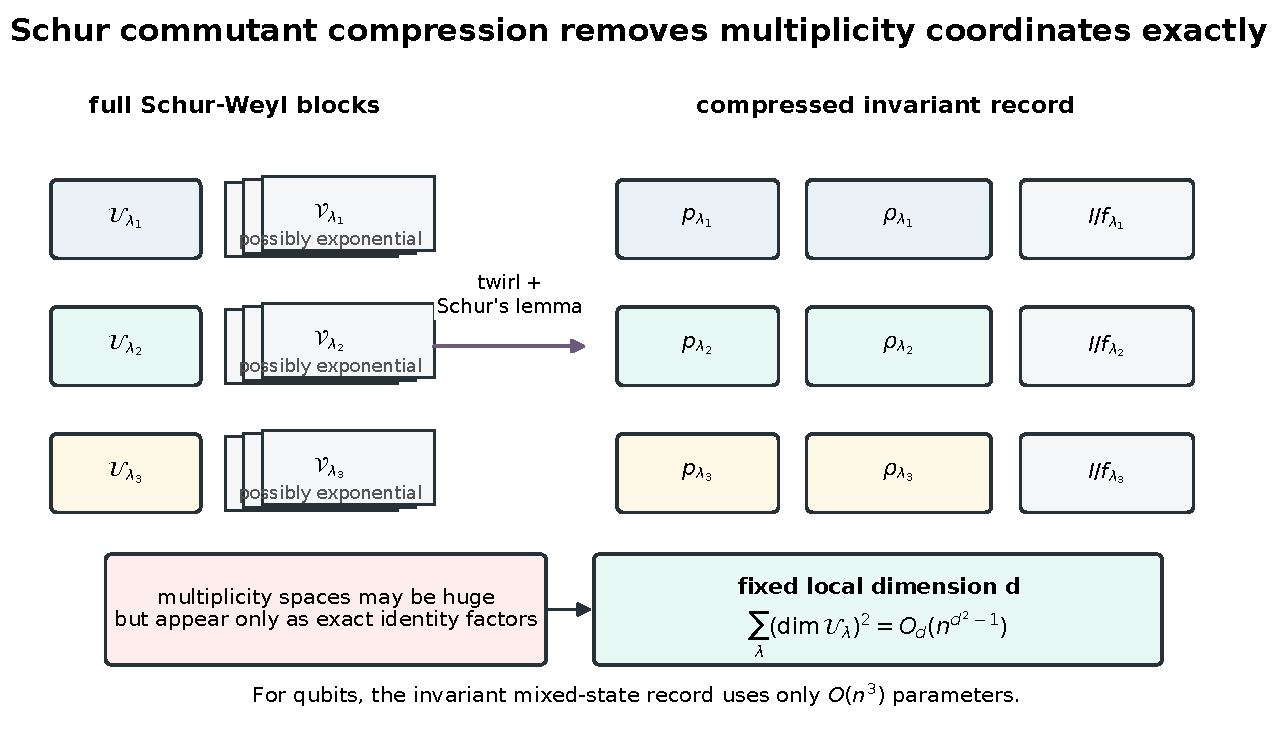
\includegraphics[width=.94\textwidth]{assets/s_schur_commutant_compression.pdf}
\caption{Permutation-invariant density operators retain the polynomial carrier blocks and replace each possibly exponential multiplicity space by an exact identity factor.}
\end{figure}

\subsection{What this theorem does not cover}
The theorem does not make an arbitrary local circuit easy. A gate acting on one selected pair generally fails to commute with all permutations. An arbitrary input may have Schur blocks that are difficult to compute from its succinct description. A non-invariant measurement can read information stored in multiplicity coordinates. Finally, allowing local dimension $d$ to grow with $n$ can make the commutant record superpolynomial.

The result is therefore a complete collapse theorem for a declared symmetry and access model, not a claim that Schur--Weyl decomposition alone solves generic many-body simulation.

\section{Orbit-quotient quantum walks}
\label{s:ch:orbit-quotients}
\index{quantum walk}
\index{orbit quotient}

\subsection{Orbit states}
Let a group $G$ act by automorphisms on a finite graph with vertex set $V$. The orbits are $\mathcal O_1,\ldots,\mathcal O_r$. Define normalized orbit states
\[
\ket{\mathcal O_a}
=
\frac1{\sqrt{|\mathcal O_a|}}
\sum_{x\in\mathcal O_a}\ket x.
\]
If the adjacency or Hamiltonian $H$ commutes with the group action, the span of these states is invariant whenever the partition is equitable.

The quotient matrix is
\[
\widetilde H_{ab}
=
\bra{\mathcal O_a}H\ket{\mathcal O_b}.
\]

\begin{theorem}[Orbit-quotient collapse]
\label{s:thm:orbit-collapse}
Suppose a uniformly described quantum walk has a polynomial number $r(n)$ of relevant orbits, an orbit-uniform initial state, an orbit-invariant final measurement, and polynomial-time algorithms for orbit sizes, quotient entries, initial orbit coordinates, and the restricted final measurement. For continuous-time evolution, also assume a polynomial bound on $|t|\|\widetilde H\|$ and efficient entry access to the precision required by the simulation. Then the walk can be simulated classically in polynomial time by the $r(n)\times r(n)$ quotient dynamics.
\end{theorem}

\begin{proof}
The orbit-state span is invariant. The state is represented by $r(n)$ amplitudes. Polynomial-time computation of quotient entries and ordinary polynomial-precision linear algebra satisfy \cref{s:thm:poly-packet}.
\end{proof}

\subsection{Hypercube example}
The $n$-dimensional hypercube is invariant under coordinate permutations. Its vertex orbits are Hamming-weight layers $0,1,\ldots,n$. In the normalized orbit basis, the quotient adjacency has couplings
\begin{equation}
\bra{k+1}A\ket{k}
=
\sqrt{(k+1)(n-k)}.
\label{s:eq:hypercube-coupling}
\end{equation}
Thus a walk on $2^n$ vertices initialized at $0^n$ evolves in an $(n+1)$-dimensional subspace.

\begin{figure}[H]
\centering
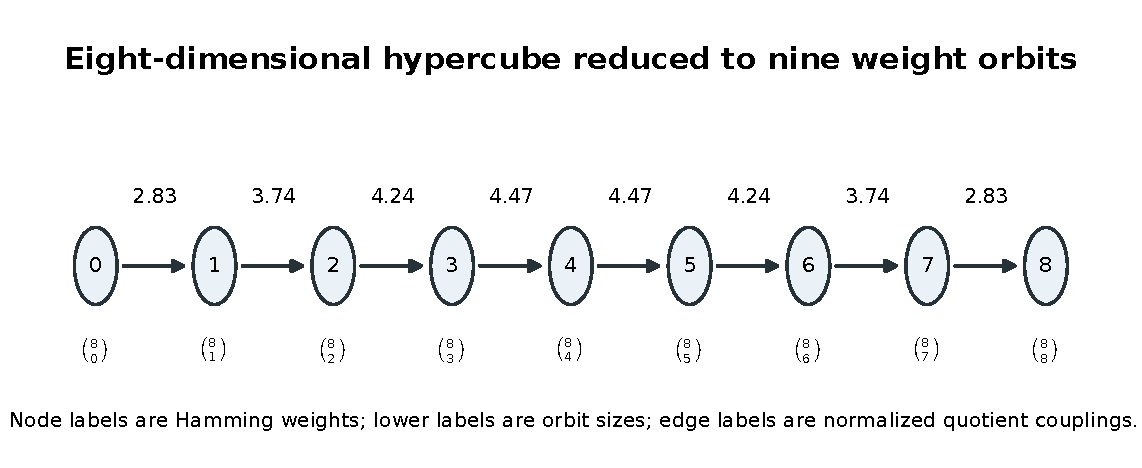
\includegraphics[width=.94\textwidth]{assets/s_hypercube_quotient.pdf}
\caption{The hypercube walk collapses to a weighted path of Hamming-weight orbits.}
\end{figure}

\subsection{The succinct-input caveat}
If the full graph is supplied explicitly, a polynomial-in-$|V|$ algorithm may still be exponential in the succinct parameter $n$. The theorem requires quotient data computable directly from the succinct graph description. Discovering graph automorphisms or orbit partitions can itself be difficult. For regular families such as hypercubes, Johnson graphs, association schemes, and Cayley graphs with known character theory, the quotient is explicit.

\subsection{Fourier packets}
On a cycle, translation characters diagonalize the adjacency operator. The continuous-time walk
\[
\ket{\psi(t)}=e^{-itA}\ket0
\]
is a sum of Fourier-character packets. This is the same discrete Fourier transform that appears as a signal-processing coordinate change, a group-character decomposition, and a quantum basis transformation.

\section{Few bosons and few fermions}
\label{s:ch:few-particles}
\index{boson}
\index{fermion}

\subsection{Bosonic occupation space}
For $N$ indistinguishable bosons in $m$ modes, a Fock basis state is an occupation vector
\[
(n_1,\ldots,n_m),
\qquad
n_1+\cdots+n_m=N.
\]
The dimension is
\begin{equation}
D_{\rm boson}(m,N)
=
\binom{N+m-1}{N}.
\label{s:eq:boson-dim}
\end{equation}
For fixed $N$, this is $O(m^N)$.

\subsection{Fermionic occupation space}
For $N$ fermions in $m$ modes, each mode is occupied at most once and
\begin{equation}
D_{\rm fermion}(m,N)
=
\binom mN.
\label{s:eq:fermion-dim}
\end{equation}
For fixed $N$, this is also polynomial in $m$.

\begin{corollary}[Few-particle collapse]
A polynomial-size number-preserving bosonic or fermionic circuit with a fixed number of particles is classically polynomial-time simulable if its initial occupation coordinates, mode-gate updates, and final observable are computable in polynomial time in the occupation basis.
\end{corollary}

\begin{proof}
Use \cref{s:eq:boson-dim,s:eq:fermion-dim} and \cref{s:thm:poly-packet}.
\end{proof}

\begin{figure}[H]
\centering
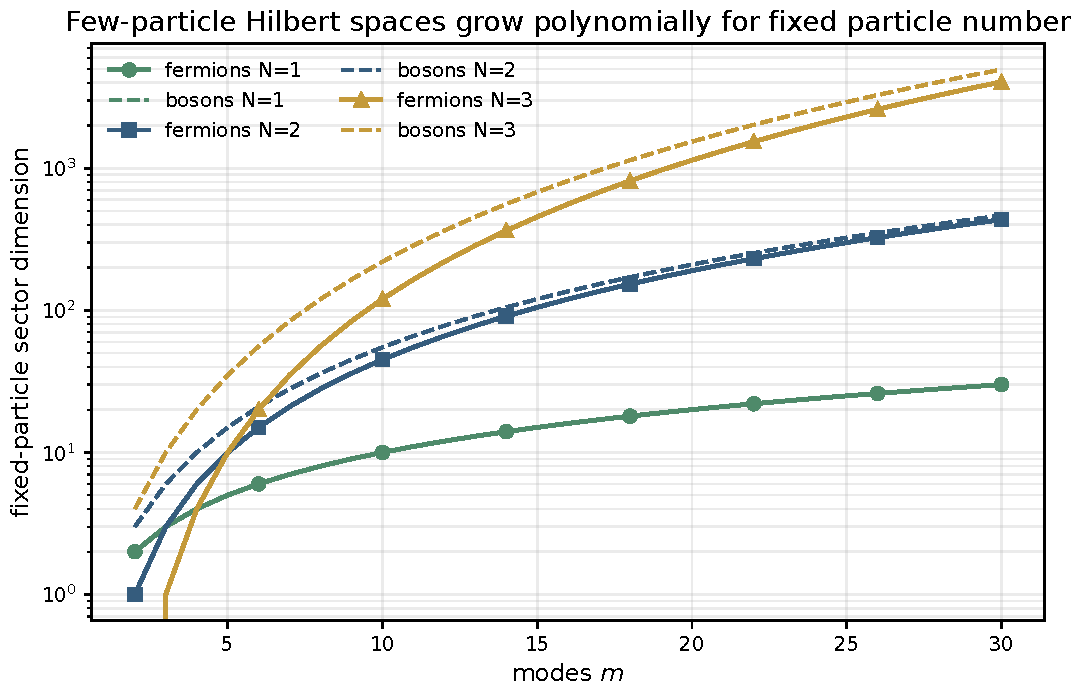
\includegraphics[width=.82\textwidth]{assets/s_few_particle_dimensions.pdf}
\caption{Fixed-particle bosonic and fermionic sectors grow polynomially with the number of modes.}
\end{figure}

\subsection{Gate updates}
A number-preserving one-body unitary acts on mode creation operators by
\[
a_i^\dagger
\longmapsto
\sum_j U_{ji}a_j^\dagger.
\]
A generic dense mode transformation can induce many occupation-basis transitions, but for fixed $N$ the basis dimension remains polynomial. Local hopping and phase gates are sparse. Few-body interactions remain polynomial to apply for fixed $N$, although the exponent can grow with $N$.

\subsection{Where the theorem stops}
If $N$ scales linearly with $m$, both dimensions become exponential. The fixed-number symmetry still reduces the full Fock space, but it does not prove polynomial simulation. Boson-sampling-type interference also shows that a fixed total particle number is not enough when the particle count itself scales with input size and the output asks for detailed many-body amplitudes.

\begin{scopebox}
The corollary is a fixed-particle theorem. It is not a claim that general many-boson or many-fermion quantum dynamics are classically easy.
\end{scopebox}

\section{Scaling phase diagrams for charge, particles, and local dimension}
\label{s:ch:scaling-phases}
\index{particle-number scaling}
\index{quasipolynomial simulation}
\index{subexponential simulation}

\subsection{Exact sector size is a complexity phase variable}
The statement ``fixed particle number is polynomial'' has a sharp extension. Let the particle number depend on the system size:
\[
k=k(n).
\]
The explicit-amplitude simulation cost of one fermionic or qubit weight packet is governed by
\[
D_{n,k}=\binom nk.
\]
For $1\le k\le n$, the standard bounds
\begin{equation}
\left(\frac nk\right)^k
\le
\binom nk
\le
\left(\frac{en}{k}\right)^k
\label{s:eq:binomial-basic-bounds}
\end{equation}
show that the growth changes continuously between polynomial and exponential regimes.

Because
\[
\binom nk=\binom n{n-k},
\]
write
\[
r(n)=\min\{k(n),n-k(n)\}.
\]

\begin{theorem}[Explicit fixed-charge phase diagram]
\label{s:thm:charge-phase-diagram}
For explicit amplitude storage in a weight-$k(n)$ packet:
\begin{enumerate}
\item the packet dimension is polynomial in $n$ if $r(n)=O(1)$;
\item the packet dimension is superpolynomial whenever $r(n)\to\infty$;
\item if $r(n)=O(\log n)$, then
\[
D_{n,k}=2^{O((\log n)^2)},
\]
so the explicit packet simulation is quasipolynomial;
\item if $r(n)=O(n^\alpha)$ for a fixed $0<\alpha<1$, then
\[
D_{n,k}=2^{O(n^\alpha\log n)},
\]
which is subexponential;
\item if $k(n)/n\to p\in(0,1)$, then
\[
\log_2 D_{n,k}
=
nH_2(k(n)/n)+O(\log n)
=
nH_2(p)+o(n),
\]
where $H_2$ is binary entropy, and the packet remains exponential.
\end{enumerate}
\end{theorem}

\begin{proof}
The upper bounds follow from \cref{s:eq:binomial-basic-bounds}. If $r=O(1)$, then $\binom nr=O(n^r)$. Conversely, suppose $r\to\infty$ and $r\le n/2$. If $r\le\sqrt n$, then
\[
\log\binom nr
\ge
r\log(n/r)
\ge
\frac r2\log n,
\]
whose ratio to $\log n$ diverges. If $r>\sqrt n$, then
\[
\log\binom nr
\ge
r\log2
\ge
\sqrt n\log2,
\]
which also dominates every constant multiple of $\log n$. For the final assertion, $p_n=k(n)/n$ stays in a compact subinterval of $(0,1)$. Stirling's formula gives
\[
\log_2\binom n{k(n)}
=nH_2(p_n)-\frac12\log_2\!\bigl(2\pi n p_n(1-p_n)\bigr)+O(1/n).
\]
The logarithmic term is $O(\log n)$, uniformly on that subinterval. Continuity of $H_2$ gives $nH_2(p_n)=nH_2(p)+o(n)$. Replacing $p_n$ by its limit inside an $O(\log n)$ estimate would require a convergence rate, which is not assumed here.
\end{proof}

\begin{derivedbox}
For the explicit occupation-amplitude representation, ``few particles'' means a bounded number of particles or holes. A slowly growing charge can still improve on full state-vector scaling, but it no longer guarantees membership in $P$.
\end{derivedbox}

\subsection{A bounded-excitation hierarchy}
The union of the first $K$ weight sectors has dimension
\[
D_{\le K}(n)
=
\sum_{k=0}^{K}\binom nk.
\]
For fixed $K$,
\[
D_{\le K}(n)=O(n^K).
\]
If $K=O(\log n)$, the same union is quasipolynomial. This refines \cref{s:cor:bounded-excitation-collapse}: bounded symmetry breaking preserves polynomial simulation, while logarithmically growing excitation gives a controlled quasipolynomial regime.

\subsection{Bosonic and fermionic analogues}
For $N$ fermions in $m$ modes,
\[
D_{\mathrm F}(m,N)=\binom mN.
\]
For $N$ bosons in $m$ modes,
\[
D_{\mathrm B}(m,N)=\binom{m+N-1}{N}.
\]
The same binomial analysis gives:

\begin{corollary}[Few-particle scaling]
\label{s:cor:few-particle-scaling}
With the number of modes as the input-size parameter:
\begin{enumerate}
\item fixed $N$ gives polynomial explicit-amplitude simulation;
\item $N=O(\log m)$ gives quasipolynomial sector size;
\item $N=O(m^\alpha)$, $0<\alpha<1$, gives subexponential sector size;
\item finite-density fermionic sectors remain exponential.
\end{enumerate}
For bosons, the statements hold in the dilute regime with the same occupation-basis access assumptions.
\end{corollary}

The adjective ``polynomial'' here refers to the sector dimension and efficient gate action. It does not assert that every interacting Hamiltonian has efficiently computable matrix elements or that every compact description remains closed.

\subsection{Symmetric qudits with growing local dimension}
The symmetric $d$-level subspace has dimension
\[
S(n,d)
=
\binom{n+d-1}{d-1}.
\]
For fixed $d$, this is polynomial in $n$. If $d=d(n)$ grows, the same phase transition appears.

\begin{proposition}[Growing-local-dimension boundary]
\label{s:prop:growing-d-boundary}
In the explicit occupation basis:
\begin{enumerate}
\item fixed $d$ gives $S(n,d)=O(n^{d-1})$;
\item $d=O(\log n)$ gives $S(n,d)=2^{O((\log n)^2)}$;
\item unbounded $d$ is not covered by the fixed-$d$ polynomial-collapse theorem without an additional internal compression.
\end{enumerate}
\end{proposition}

Thus permutation symmetry removes the exponential tensor-product multiplicity only when the number of local levels is controlled, or when the occupation record itself admits a second compression.

\begin{figure}[H]
\centering
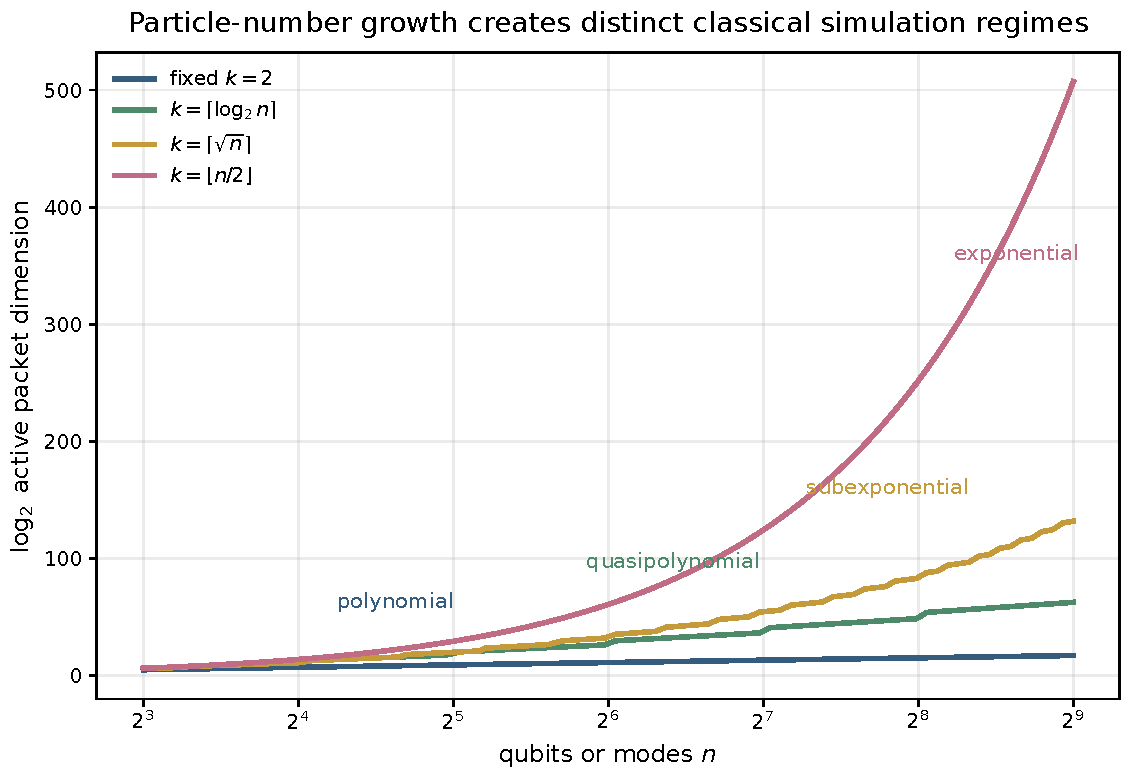
\includegraphics[width=.94\textwidth]{assets/s_particle_scaling_phases.pdf}
\caption{The active dimension passes through polynomial, quasipolynomial, subexponential, and exponential regimes as particle number grows.}
\end{figure}

\subsection{Complexity class versus practical runtime}
A polynomial sector can still have a large exponent. Fixed $k=20$ gives $O(n^{20})$ explicit amplitudes, which is in $P$ but may be impractical. Conversely, a subexponential sector may be useful at moderate size without changing the formal complexity class.

A complete performance claim should therefore report both:
\[
\text{asymptotic class}
\qquad\text{and}\qquad
\text{actual representation size and update cost}.
\]
This is why the benchmark chapters keep wall-clock evidence separate from the dimension theorems.

\section{Stabilizer syndromes and Clifford packets}
\label{s:ch:stabilizer}
\index{stabilizer}
\index{Clifford circuit}

\subsection{Syndrome projectors}
Let $S_1,\ldots,S_m$ be commuting Pauli stabilizers with eigenvalues $\pm1$. A syndrome $s\in\{0,1\}^m$ defines
\[
P_s
=
\prod_{j=1}^m
\frac{I+(-1)^{s_j}S_j}{2}.
\]
These projectors are orthogonal and sum to the identity. Syndrome measurement selects one packet, while recovery applies a syndrome-dependent transfer toward the code packet.

\subsection{The syndrome label is not the logical state}
If the code encodes $k$ logical qubits, a fixed syndrome packet can have dimension $2^k$. The syndrome has only $m$ bits, but arbitrary logical information remains inside the packet. Syndrome packetization therefore does not by itself prove efficient simulation.

\subsection{Tableau compression}
Clifford circuits provide a different route. A stabilizer state may occupy exponentially many computational-basis strings, yet it is represented by a polynomial-size stabilizer tableau. Clifford gates update the tableau in polynomial time, and Pauli measurements are efficiently computable. This is an example of the compressed-packet theorem rather than a small-dimensional packet theorem.

\begin{derivedbox}
Packet labels and internal encoding are complementary. A Clifford circuit restricted to selected syndromes may be simulated by a tableau augmented with the active syndrome graph, even when the packet dimensions are exponential.
\end{derivedbox}

\subsection{Non-Clifford residues}
A few non-Clifford gates can be handled by stabilizer decompositions, quasiprobability expansions, or magic-state rank methods. The cost grows with a non-Clifford resource such as stabilizer rank or robustness. Symmetry packets may reduce the number of relevant branches, but they do not eliminate the intrinsic cost of the non-Clifford residue.

\subsection{Error-correction interpretation}
The packet view separates three objects:
\[
\text{syndrome label},
\qquad
\text{logical state},
\qquad
\text{recovery transfer}.
\]
This separation is useful for compressed simulation of fault-tolerant protocols, but a full complexity statement must include repeated measurements, classical control, and the size of the logical state.

\section{Gaussian, fermionic, and matchgate compression}
\label{s:ch:gaussian}
\index{Gaussian circuit}
\index{matchgate}

\subsection{Polynomial covariance representations}
Gaussian bosonic and fermionic states are specified by first and second moments rather than by all Fock-basis amplitudes. A bosonic covariance matrix has size polynomial in the number of modes, and a fermionic Gaussian state is represented by an antisymmetric Majorana covariance matrix. Gaussian unitaries act by symplectic or orthogonal transformations:
\[
\Gamma\longmapsto S\Gamma S^T
\quad\text{or}\quad
\Gamma\longmapsto O\Gamma O^T.
\]
This is a compact internal encoding even when the corresponding Hilbert-space packet is exponentially large.

\subsection{Hybrid symmetry and Gaussianity}
Number conservation, parity, translation symmetry, and point-group symmetry can further block the covariance matrices. A simulator can therefore combine two reductions:
\[
\text{symmetry packetization}
+
\text{Gaussian internal encoding}.
\]
The first removes unreachable sectors. The second compresses states within the remaining sectors.

\subsection{Matchgate circuits}
Nearest-neighbor matchgate circuits have polynomial classical representations through fermionic Gaussian dynamics. Geometry matters: adding SWAP, fermionic SWAP, long-range gates, or a non-matchgate resource changes the simulation problem. A symmetry-collapse atlas should therefore record the gate library and connectivity as part of the model, not as implementation details.

\subsection{Low-rank non-Gaussian corrections}
One research direction is to represent a weakly non-Gaussian state as
\[
\rho
=
\sum_{a=1}^R c_a\rho_a^{\rm Gauss}
\]
with small Gaussian rank $R$, or as a Gaussian reference plus sparse packet corrections. A polynomial collapse requires $R$ and the update cost to remain polynomial.

\begin{frontierbox}
Gaussianity is an internal representation class, not a symmetry projector. A complete hybrid theorem must prove closure of the chosen compressed class under every allowed gate and bound the growth of any non-Gaussian residue.
\end{frontierbox}

\subsection{Few-particle versus Gaussian routes}
Fixed-particle simulation and Gaussian simulation are independent. A fixed two-fermion state may be non-Gaussian but live in a polynomial-dimensional sector. A half-filled Gaussian state may live in an exponential number sector but have a polynomial covariance description. The two-axis model in \cref{s:ch:compressed-packets} is designed to capture this distinction.

\chapter{States, measurements, and open dynamics}
\section{Density operators: populations and coherences}
\label{s:ch:density}
\index{density operator}
\index{coherence}

\subsection{Two packet indices}
A pure state uses one packet label. A density operator uses two:
\[
\rho
=
\sum_{\alpha,\beta}
P_\alpha\rho P_\beta.
\]
The diagonal block $P_\alpha\rho P_\alpha$ is population inside packet $\alpha$. The off-diagonal block $P_\alpha\rho P_\beta$ is coherence between packets $\alpha$ and $\beta$.

Discarding off-diagonal blocks is not merely a change of coordinates. It is a physical operation such as dephasing. An exact simulator must preserve all coherence blocks relevant to the final observable.

\subsection{Hilbert--Schmidt decomposition}
Orthogonality of the left-right operator packets gives
\[
\|\rho\|_2^2
=
\sum_{\alpha,\beta}
\|P_\alpha\rho P_\beta\|_2^2.
\]
This identity supplies an exact coherence-energy ledger. It can be used to decide which blocks are large, to audit dephasing, or to bound truncation errors in approximate packet simulations.

\subsection{Symmetry-preserving unitary dynamics}
If $U$ commutes with every packet projector, then
\[
P_\alpha U\rho U^\dagger P_\beta
=
U(P_\alpha\rho P_\beta)U^\dagger.
\]
The left and right packet labels are preserved. Populations and coherences evolve independently by their declared labels.

\subsection{Observable sparsity}
For an observable $M$,
\[
\Tr(M\rho)
=
\sum_{\alpha,\beta}
\Tr(P_\beta M P_\alpha\,P_\alpha\rho P_\beta).
\]
Only operator packets coupled by $M$ contribute. A measurement that is diagonal in the symmetry labels depends only on populations. A phase-sensitive measurement can require off-diagonal coherences.

\begin{figure}[H]
\centering
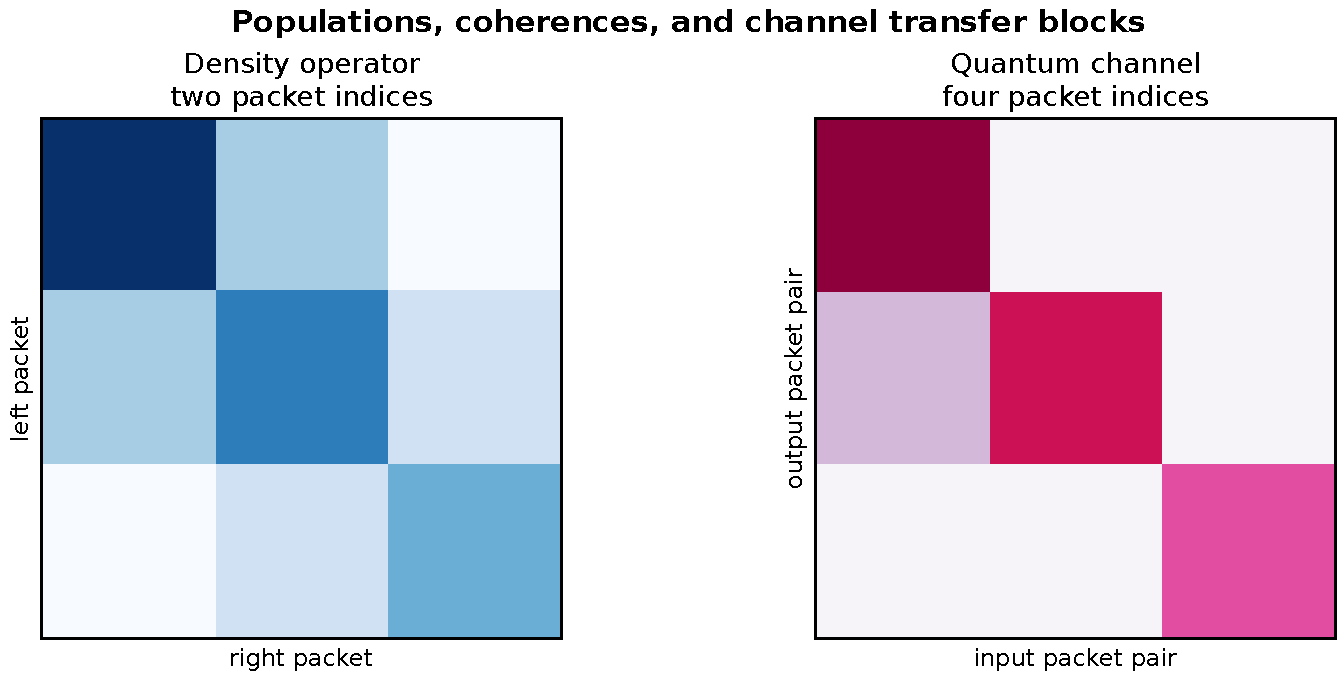
\includegraphics[width=.78\textwidth]{assets/s_channel_blocks.pdf}
\caption{State operators carry two packet indices, while channels act between pairs of packet labels.}
\end{figure}

\subsection{Polynomial operator-space collapse}
If only polynomially many density blocks are reachable and every block has a polynomial representation, then mixed-state evolution can also be simulated in polynomial time. The representation size is not the square of the full Hilbert dimension. It is the total cost of the active left-right blocks.

\begin{derivedbox}
For a polynomial active set $A_n$ of packet labels, a density-matrix simulator has at most $|A_n|^2$ label pairs. Polynomial-time simulation follows when each active coherence block has a polynomial classical representation and channel updates remain sparse and efficient.
\end{derivedbox}

\section{Channels, Kraus maps, and Lindblad generators}
\label{s:ch:channels}
\index{quantum channel}
\index{Lindblad equation}

\subsection{Four-index transfer}
A quantum channel with Kraus operators $K_\mu$ acts by
\[
\Phi(\rho)
=
\sum_\mu K_\mu\rho K_\mu^\dagger.
\]
Relative to operator packets
\[
\mathcal P_{\alpha\beta}(X)
=
P_\alpha X P_\beta,
\]
the channel has blocks
\[
\Phi_{\gamma\delta,\alpha\beta}
=
\mathcal P_{\gamma\delta}
\,\Phi\,
\mathcal P_{\alpha\beta}.
\]
Thus a channel carries four packet labels: an input coherence pair and an output coherence pair.

\subsection{Symmetry-preserving channels}
If every Kraus operator commutes with the symmetry action, the channel is diagonal in the isotypic labels. More generally, Kraus operators may carry definite charges, producing a sparse selection rule. Amplitude damping transfers population between number sectors. Dephasing damps selected off-diagonal blocks. Particle loss moves weight-$k$ population to weight $k-1$.

\subsection{Lindblad dynamics}
A Markovian open system obeys
\[
\frac{d\rho}{dt}
=
\mathcal L(\rho)
=
-i[H,\rho]
+
\sum_a
\left(
L_a\rho L_a^\dagger
-
\frac12\{L_a^\dagger L_a,\rho\}
\right).
\]
Packet selection rules of $H$ and $L_a$ determine a sparse directed graph on coherence pairs. If the reachable graph and each block representation remain polynomial, a classical integrator can evolve the reduced system.

\subsection{Error accounting for truncated channels}
Let $\Pi_A$ project operator space onto an active set of coherence blocks. A reduced evolution uses
\[
\mathcal L_A
=
\Pi_A\mathcal L\Pi_A.
\]
The discarded transfer is
\[
(I-\Pi_A)\mathcal L\Pi_A.
\]
Duhamel's formula yields an error bound analogous to the Hamiltonian leakage theorem. The resulting estimate depends on the induced norm of the discarded superoperator transfer and the integration time.

\subsection{Syndrome-conditioned recovery}
Error correction naturally fits the four-index model. Syndrome measurement selects a population packet, classical processing chooses a recovery, and the recovery transfers the state toward the code packet. A full simulation must still retain the logical state inside each syndrome sector.

\begin{frontierbox}
A useful open-system collapse theorem should state the norm, time horizon, packet-discovery algorithm, integration precision, and growth of reachable coherence pairs. Sparsity of a displayed block matrix is not enough by itself.
\end{frontierbox}

\section{Measurement, conditioning, and classical feedback}
\label{s:ch:measurement}
\index{measurement}

\subsection{Projective measurement}
For projectors $\{P_\alpha\}$, the probability of outcome $\alpha$ is
\[
p_\alpha
=
\Tr(P_\alpha\rho),
\]
and the conditioned state is
\[
\rho_\alpha
=
\frac{P_\alpha\rho P_\alpha}{p_\alpha}
\]
when $p_\alpha>0$. Measurement is therefore packet selection followed by normalization.

\subsection{Branching complexity}
A measurement-assisted circuit produces a tree of outcomes. Classical simulation is efficient when the branch distribution can be sampled or summed without enumerating exponentially many relevant histories. Symmetry can merge histories that lead to the same packet state, but only if the feedforward policy respects the same equivalence.

\subsection{Dynamic programming on packet states}
Suppose each branch is represented by a pair $(\alpha,r)$, where $\alpha$ is a packet label and $r$ is a compact internal state. If polynomially many distinct pairs occur at every depth, identical pairs can be merged and their probabilities added. This gives a dynamic program instead of an exponential branch tree.

\begin{proposition}[Branch-merging simulation]
Suppose a measurement-and-feedback circuit has polynomial depth and polynomially many distinct reachable packet representations at each step. Assume that the initial representation is efficiently constructible, each representation has a polynomial-time canonical key sufficient for all future transitions, all successor representations and their transition probabilities can be enumerated in polynomial time, and the final predicate is efficient. Then the final acceptance probability is classically computable to the requested polynomial precision in polynomial time. The same conclusion holds for any polynomially supported final output distribution.
\end{proposition}

\begin{proof}
Maintain a probability dictionary over distinct packet representations. Each measurement or controlled gate updates every entry into polynomially many successors. Merge equal successors. The dictionary remains polynomial by hypothesis.
\end{proof}

\subsection{Reset and dissipation}
Reset is nonunitary but often simplifies a classical representation by removing entropy or closing branches. Conversely, measurement may expose a classical label while leaving a complex logical state. The resource value of measurement depends on the target, ancilla convention, and cost function.

\subsection{Connection to catalytic gate models}
The larger gate-set monograph studies temporary excursions into measurement, ancilla, or symmetry-breaking resources. The present monograph asks a different question: when does the resulting model remain classically simulable? A temporary resource may shorten a quantum circuit without making the computation classically easy.

\section{Block encodings and polynomial operator transforms}
\label{s:ch:block-encodings}
\index{block encoding}

\subsection{Projector block form}
A block encoding places a generally nonunitary operator $A$ inside a larger unitary $U$ so that
\[
(\bra0\otimes I)
U
(\ket0\otimes I)
=
\frac{A}{\alpha}.
\]
With
\[
P_0=\ket0\bra0\otimes I,
\]
this is the selected block
\[
P_0UP_0
=
\frac{A}{\alpha}
\]
after identifying the encoded subspace.

\subsection{Structural connection}
The encoded operator is literally a projector block of a unitary. Polynomial transformations of singular values can be implemented by controlled phase sequences once the block encoding and access model are available. This makes block encodings a natural part of a projector calculus.

\subsection{Why block encoding does not imply classical simulation}
A block encoding can be efficient on a quantum computer because $U$ is supplied by an oracle or a succinct circuit. A classical algorithm may not have efficient access to the entries of $A$, to the block state, or to the polynomial transform. The selected block may still have exponential dimension.

\begin{scopebox}
The statement ``$A$ is a block of $U$'' is structural. A classical collapse requires a polynomial classical description of the active encoded state, efficient application of the selected block, and efficient evaluation of the output.
\end{scopebox}

\subsection{Symmetry-resolved block encodings}
If $A$ commutes with a symmetry group, both the encoded system and the ancilla can be decomposed into packets. A symmetry-resolved block encoding may reduce normalization, memory, or simulation cost for selected sectors. The relevant objects are
\[
P_\chi P_0 U P_0P_\psi.
\]
Exact symmetry removes off-diagonal $\chi\neq\psi$ blocks. Approximate symmetry yields leakage terms that must be included in the error budget.

\subsection{Research direction}
A useful classical theorem would identify access models in which the active block has polynomial packet dimension or a compact internal representation. This could cover structured sparse matrices, low-rank updates, association-scheme operators, and fixed-particle Hamiltonians.

\chapter{The complexity boundary}
\section{Compressed packet simulation}
\label{s:ch:compressed-packets}
\index{compressed representation}

\subsection{Beyond packet dimension}
The small-packet theorem stores one amplitude per packet-basis state. This is not the only classical representation. A state in an exponentially large packet may lie on a polynomially parameterized manifold. Stabilizer states, Gaussian states, matrix-product states of bounded bond dimension, and low-rank operator states are standard examples of compact internal encodings.

Let $\mathcal R_n$ be a class of classical descriptions, and let
\[
\operatorname{decode}:\mathcal R_n\to P_n\Hh_n
\]
associate a quantum state with each description.

\begin{theorem}[Compressed-packet simulation]
\label{s:thm:compressed-packet}
A polynomial-time uniform quantum circuit family lies in $P$ if there is a polynomial-size classical representation satisfying:

\begin{enumerate}
\item the initial state has an efficiently constructible description $r_0\in\mathcal R_n$;
\item every gate induces a polynomial-time update $r\mapsto T_j(r)$ with
\[
\operatorname{decode}(T_j(r))
=
G_j\operatorname{decode}(r);
\]
\item all intermediate description sizes remain polynomial;
\item the acceptance probability is computable from the final description in polynomial time.
\end{enumerate}
\end{theorem}

\begin{proof}
Iterate the polynomial-time classical updates on the polynomial-size descriptions and evaluate the final measurement. The algorithm never reconstructs the full state vector.
\end{proof}

\subsection{Two-axis complexity}
The records suggest the pair
\[
(D_{\rm packet},\chi_{\rm internal}),
\]
where $D_{\rm packet}$ measures active packet size or count and $\chi_{\rm internal}$ measures the representation cost inside the packet. Efficient simulation may follow from either coordinate:

\begin{itemize}
\item fixed weight has polynomial $D_{\rm packet}$ and can use explicit amplitudes;
\item stabilizer states may have exponential support but polynomial $\chi_{\rm internal}$;
\item Gaussian states may occupy large number sectors but have polynomial covariance descriptions;
\item half-filled generic states may have both coordinates exponential.
\end{itemize}

\begin{figure}[H]
\centering
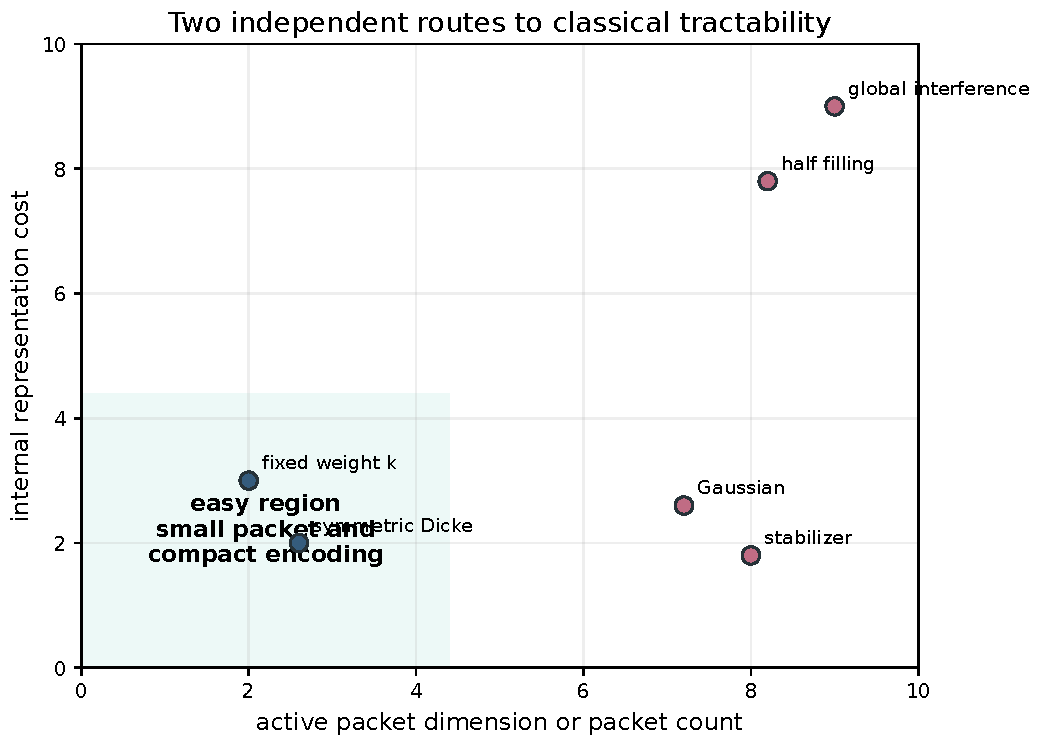
\includegraphics[width=.72\textwidth]{assets/s_two_axis_complexity.pdf}
\caption{Packet dimension and internal representation cost are independent classical resources.}
\end{figure}

\subsection{Hybrid transfer graphs}
Suppose packets are nodes of a sparse graph and each node carries an internal representation. A gate may update a node internally or transfer a compact component to neighboring nodes. The simulation cost depends on
\[
\sum_{\alpha\in A_t}\operatorname{size}(r_\alpha)
+
\#\{\text{nonzero transfers at time }t\}.
\]
This model combines symmetry selection rules with compact state classes.

\subsection{Closure is the decisive condition}
A compact representation may be destroyed by one gate. Clifford tableaux fail under generic non-Clifford rotations. Gaussian covariance matrices fail under generic non-Gaussian operations. Low-bond tensor networks may acquire exponential bond dimension. The theorem therefore requires closure or a proved polynomial growth bound, not merely a compact initial state.

\begin{principle}[Representation growth audit]
The correct complexity variable is the maximum representation size reached along the computation, not the size of the initial or final state alone.
\end{principle}

\section{Global interference and the failure of local packet collapse}
\label{s:ch:global-interference}
\index{Forrelation}
\index{interference}

\subsection{A different quantum mechanism}
Invariant-packet reduction succeeds when large parts of Hilbert space are never occupied or can be compressed locally. A different regime stores the answer in coherent relations among many paths. The individual amplitudes may be simple, while their signed sum is the computational object.

\subsection{Forrelation amplitude}
Let $f,g:\{0,1\}^n\to\{-1,1\}$ and $N=2^n$. The circuit with alternating Hadamards and phase oracles has zero-state amplitude
\begin{equation}
\Phi(f,g)
=
\frac1{N^{3/2}}
\sum_{x,y}
 f(x)(-1)^{x\cdot y}g(y).
\label{s:eq:forrelation}
\end{equation}
The circuit does not evaluate the $N^2$ terms separately. It preserves phases and lets them interfere.

\begin{figure}[H]
\centering
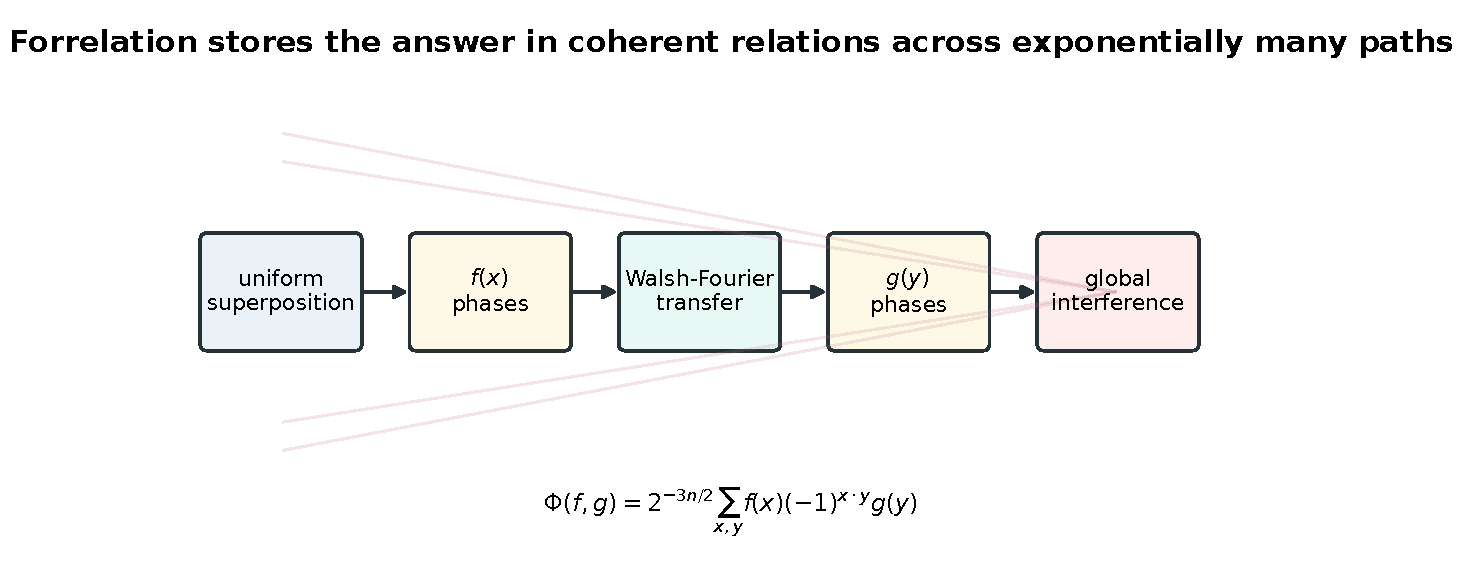
\includegraphics[width=.90\textwidth]{assets/s_forrelation_interference.pdf}
\caption{Forrelation is governed by coherent Fourier transfer rather than a small invariant sector.}
\end{figure}

\subsection{Why Fourier structure is not automatically easy}
The Walsh transform is explicit and highly symmetric. That does not imply that the bilinear expression in \cref{s:eq:forrelation} is classically polynomial-time computable when $f$ and $g$ are supplied through restricted query access. The difficulty lies in the access model and the coherent global relation, not in the absence of algebraic structure.

\subsection{Truth tables versus succinct access}
If the complete truth tables of $f$ and $g$ are part of the classical input, their length is already $N$, and an $O(N\log N)$ Walsh transform is polynomial in the explicit input length. In a query or succinct-circuit model, $n$ is the parameter and $N=2^n$. The same formula then represents exponentially many values.

This distinction illustrates a general rule: complexity statements must be measured against the input encoding. A quotient of exponential dimension may be efficient relative to an explicit matrix input but exponential relative to a succinct circuit input.

\subsection{Cross-packet coherence}
Suppose a projector family gives many packets $P_\alpha$. Even if each diagonal block is simple, the output can depend on the phases of
\[
P_\alpha\ket\psi
\quad\text{relative to}\quad
P_\beta\ket\psi
\]
for exponentially many pairs. A simulator that retains only populations
\[
\|P_\alpha\ket\psi\|^2
\]
loses this information. The hard-side invariant must measure classical compression of coherent relations, not merely active dimension.

\begin{frontierbox}
A representation-independent lower bound on interference compression for an explicit, succinct, uniform circuit family would be a major complexity result. The packet framework states the missing object but does not provide that lower bound.
\end{frontierbox}

\section{Simulation complexity versus decision complexity}
\label{s:ch:decision-complexity}

\subsection{Why simulator lower bounds are insufficient}
Showing that a circuit defeats one simulation strategy does not prove that its decision problem is outside $P$. A classical algorithm may compute the answer without reconstructing the quantum state. It is therefore insufficient to rule out only:

\begin{itemize}
\item full state-vector simulation,
\item one projector family,
\item bounded-width tensor-network contraction,
\item path sampling,
\item low-rank transfer matrices,
\item stabilizer decompositions,
\item any fixed catalogue of known simulators.
\end{itemize}

A proof of $P\neq BQP$ would need a lower bound against every deterministic polynomial-time classical algorithm for an explicit language.

\subsection{A representation-relative invariant}
For a declared classical representation class $\mathcal R$, define
\[
\operatorname{TC}^{\mathcal R}_\varepsilon(C)
=
\min\left\{
\operatorname{cost}(R):
R\in\mathcal R,
\ |R(C)-p_C|\le\varepsilon
\right\},
\]
where $p_C$ is the target acceptance probability. This permits a disciplined ladder:

\begin{enumerate}
\item exact polynomial-packet simulation for easy sectors;
\item lower bounds for local packet-query methods;
\item lower bounds for broader tensor, sampling, low-degree, and communication representations;
\item a representation-independent lower bound;
\item a separation of $P$ and $BQP$.
\end{enumerate}

Only the first step is completed here.

\subsection{Universal packetization and its consequence}
Consider the statement:

\begin{conjecture}[Universal polynomial packetization]
Every polynomial-time uniform quantum circuit family admits an efficiently discoverable exact or approximate packet representation of polynomial active size and polynomial transfer complexity, sufficient to compute its acceptance probability.
\end{conjecture}

If true, \cref{s:thm:poly-packet,s:thm:compressed-packet} would imply $BQP\subseteq P$, and hence $P=BQP$. The records do not establish this conjecture and explicitly identify global interference as an obstacle.

\subsection{The opposite route}
An explicit uniform family with a proved representation-independent classical lower bound and a polynomial quantum algorithm would establish $P\neq BQP$. The candidate succinct transfer-interference problem in the records illustrates the form of such a target, but the required lower bound is the unresolved theorem itself.

\begin{scopebox}
This monograph proves polynomial classical simulation for declared subclasses. It neither proves nor assumes a universal collapse of quantum computation.
\end{scopebox}

\subsection{Nonrelativizing issues}
Oracle separations show that query complexity can distinguish quantum and classical access. They also show why a black-box argument alone cannot settle ordinary $P$ versus $BQP$. A full separation would have to use explicit features such as uniform circuit generation, arithmetic structure, algebraic degree, communication constraints, or another nonrelativizing mechanism.

\section{Existence defects and quantum combinatorial realizations}
\label{s:ch:existence-defects}

\subsection{Metric collapse and existence collapse}
The simulation theorems compare costs of two realizations that both exist. A broader restricted-realization framework also allows the restricted object to be absent. If
\[
\mathcal R(x)=\varnothing,
\qquad
\mathcal A(x)\neq\varnothing,
\]
then enlarging the realization category changes feasibility rather than merely runtime.

\subsection{Quantum Latin-square example}
The order-six quantum-Latin-square record supplies an existence-level example. Entangled quantum Latin squares of order six exist, while mutually orthogonal non-entangled quantum Latin squares of order six do not. This is an ambient-versus-restricted realization gap, not a proof of classical simulation and not a gate-count shortcut.

The proof architecture uses support patterns, unitary-pattern constraints, graph orthonormal representations, projective-line closure, dimension contradictions, and a finite reduction to twelve classical Latin-square classes. Its conceptual relevance here is limited but useful: enlarging the allowed quantum resource can change whether a structure exists at all.

\subsection{Why this does not imply computational advantage}
Existence of an entangled combinatorial design does not by itself provide an algorithmic speedup. One must still specify an input problem, circuit family, output rule, and classical comparison. Likewise, nonexistence of a product realization does not prove classical hardness of the entangled realization.

\begin{scopebox}
The quantum Latin-square result is included as a contextual example of restricted-realization failure. It is not used as a premise in any packet-simulation theorem.
\end{scopebox}

\subsection{Unified terminology}
For a target $x$, let $c_{\rm res}(x)$ and $c_{\rm amb}(x)$ be minimum costs, with $+\infty$ assigned when a realization does not exist. Then
\[
\Delta(x)
=
c_{\rm res}(x)-c_{\rm amb}(x)
\]
includes both finite metric defects and infinite existence defects. Symmetry collapse concerns the special case where the ambient quantum description has a cheaper classical realization because its reachable representation is compressed.

\chapter{Algorithms and open directions}
\section{Architecture of a symmetry-collapse compiler}
\label{s:ch:compiler}
\index{compiler}

\subsection{The five-stage pipeline}
A practical compiler must perform more than symbolic block diagonalization.

\begin{enumerate}
\item Detect exact or approximate symmetries.
\item Construct an invariant basis, orbit quotient, or compact internal representation.
\item Compile each gate into that representation.
\item Track leakage, truncation, and numerical error.
\item Evaluate the requested measurement and emit a complexity certificate.
\end{enumerate}

\begin{figure}[H]
\centering
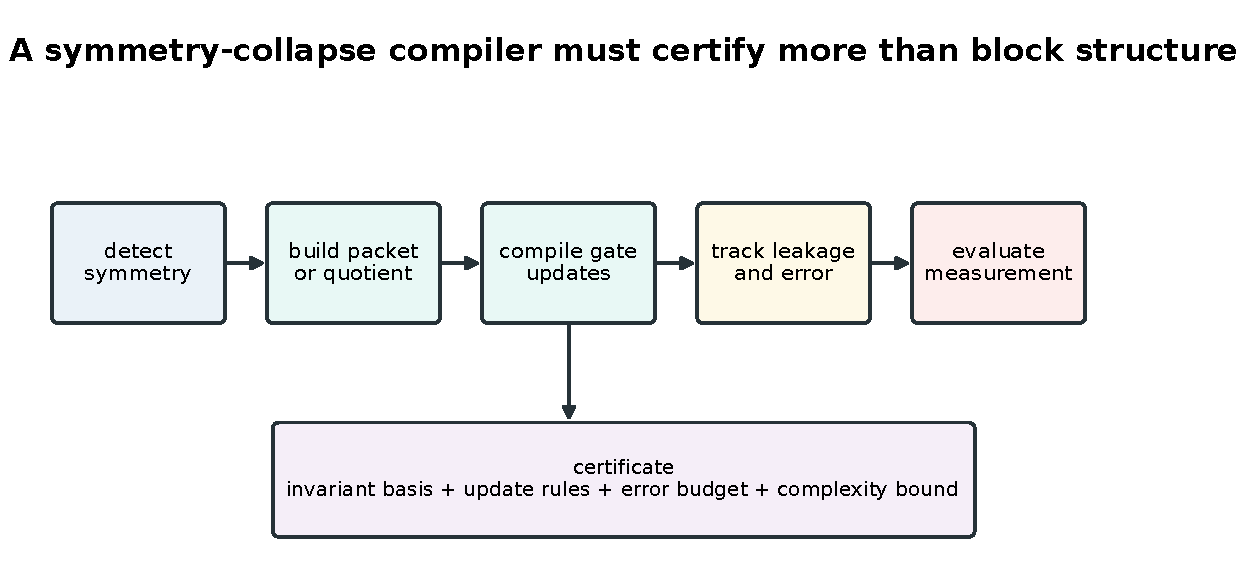
\includegraphics[width=.94\textwidth]{assets/s_compiler_pipeline.pdf}
\caption{A symmetry-collapse compiler and its required certificate.}
\end{figure}

\subsection{Symmetry detection}
Detection may use declared conserved quantities, commutators, finite-group generators, graph automorphisms, stabilizer relations, occupation conservation, or numerical approximate symmetries. Exact symbolic detection is preferable when available. Numerical detection must specify tolerances and how they propagate.

\subsection{Basis construction}
Examples include:

\begin{itemize}
\item subset indexing for fixed weight,
\item occupation vectors for bosons,
\item Dicke states for full permutation symmetry,
\item Schur coordinates for broader permutation symmetry,
\item orbit states for graph walks,
\item stabilizer tableaux,
\item fermionic or bosonic covariance matrices,
\item matrix-product states for bounded entanglement.
\end{itemize}

The compiler should avoid materializing an exponentially large change-of-basis matrix. It needs direct indexing and update formulas.

\subsection{Gate plan caching}
For a repeated circuit family, compile a packet plan containing affected index pairs, sparse matrix blocks, phase tables, and quotient couplings. The plan can be reused across parameter values when the sparsity pattern is fixed.

\subsection{Fallback and adaptive enlargement}
If a gate leaks from the current representation, the compiler can reject the reduction, merge packets, add neighboring sectors, or switch internal representations. The choice must preserve a certified error budget.

\subsection{Output certificate}
A useful machine-readable certificate should include:

\begin{itemize}
\item the symmetry or invariant-subspace proof,
\item active dimensions or representation sizes,
\item gate update complexity,
\item leakage or approximation bounds,
\item measurement complexity,
\item benchmark and hardware metadata,
\item the final complexity conclusion and its scope.
\end{itemize}

\section{Benchmark and validation protocol}
\label{s:ch:benchmark-protocol}

\subsection{Fair comparison}
A packet simulator and a full simulator should use the same precision, gate parameters, initial state, observable, and arithmetic path wherever possible. Report compilation separately from repeated application.

\subsection{Required metrics}
A complete benchmark should report:

\begin{enumerate}
\item full and reduced dimensions,
\item packet-discovery and compilation time,
\item one-shot runtime,
\item repeated-application runtime,
\item peak memory,
\item reconstruction or observable error,
\item symmetry leakage,
\item hardware and software versions,
\item number of repetitions over which compilation is amortized.
\end{enumerate}

\subsection{Algebraic and numerical validation paths}
For manageable $n$, embed a random packet state into the full space, apply identical gates in both representations, and compare final states. The included numerical validation program performs this check for structurally invariant fixed-weight circuits using complex floating-point arithmetic, with reconstruction tolerance $2\cdot10^{-12}$. The separate rational validation uses exact fractions and rational orthogonal gates. Exact subspace invariance is a property of the model, while near-machine-precision agreement is numerical evidence about this implementation.

\subsection{Scaling studies}
A scaling plot should include both fine packets and coarse packets. Fixed weight two demonstrates polynomial dimension. Parity demonstrates a constant-factor packet. Half filling demonstrates an exponential packet with a polynomial memory reduction factor. These controls prevent overinterpreting a speedup as a complexity collapse.

\subsection{Leakage tests}
Deliberately append a gate that breaks the proposed symmetry and verify that the simulator detects nonzero leakage. The archived tests break exact weight, parity, and weight modulo four, producing retained probabilities below one. A simulator that reports zero error after a symmetry-breaking gate without enlarging its representation is incorrect.

\subsection{Reproducibility contract}
The release preserves:

\begin{itemize}
\item the benchmark JSON data,
\item the Python figure generator,
\item packet and gate utilities,
\item exact rational checks and separately labeled numerical validation tests,
\item LaTeX source,
\item deterministic build commands,
\item checksums of final artifacts.
\end{itemize}

\begin{recordbox}
The release validation reproduces fixed-weight basis dimensions, residue partitions, symmetric/bosonic/fermionic dimension formulas, hypercube quotient symmetry, and full-vs-packet state reconstruction near machine precision.
\end{recordbox}

\section{Atlas of candidate symmetry collapses}
\label{s:ch:atlas}

\begin{figure}[H]
\centering
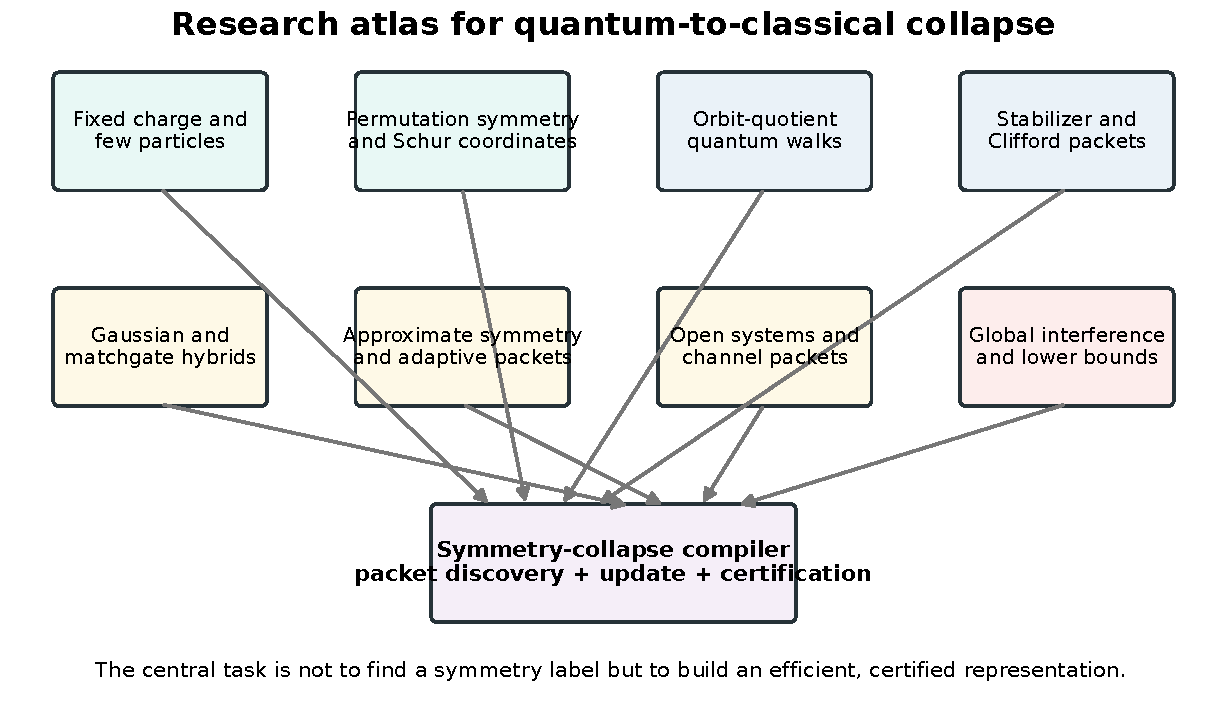
\includegraphics[width=.94\textwidth]{assets/s_research_atlas.pdf}
\caption{The main theorem and implementation directions organized around one certified compiler.}
\end{figure}

\subsection{High-confidence theorem families}
\begin{longtable}{@{}L{.25\textwidth}L{.33\textwidth}L{.32\textwidth}@{}}
\caption{High-priority collapse families.}\\
\toprule
Family & Compression mechanism & Decisive condition\\
\midrule
\endfirsthead
\toprule
Family & Compression mechanism & Decisive condition\\
\midrule
\endhead
Fixed charge $k=O(1)$ & Explicit subset basis of size $\binom nk$ & Number-preserving gates and efficient measurement\\
Permutation-symmetric qubits & Dicke basis of size $n+1$ & Collective or permutation-invariant dynamics\\
Symmetric qudits, fixed $d$ & Occupation basis $\binom{n+d-1}{d-1}$ & Efficient occupation-space updates\\
Polynomial-orbit walks & Quotient Hamiltonian on orbit states & Succinct quotient entries and orbit-invariant input/output\\
Few bosons or fermions & Fixed-particle occupation basis & Fixed particle number and efficient few-body updates\\
Stabilizer circuits & Tableau representation & Clifford closure and efficient Pauli measurement\\
Gaussian circuits & Covariance representation & Gaussian closure and efficient observable evaluation\\
\bottomrule
\end{longtable}

\subsection{Hybrid theorem targets}
The strongest new classes may combine several resources:

\begin{itemize}
\item charge packets plus Gaussian covariance,
\item permutation packets plus bounded-bond tensor networks,
\item stabilizer tableaux plus a small syndrome transfer graph,
\item orbit quotients plus Fourier diagonalization,
\item adaptive approximate packets plus rigorous leakage accounting.
\end{itemize}

\subsection{Negative controls}
A research atlas should preserve cases that do not collapse:

\begin{itemize}
\item parity alone,
\item weight modulo a fixed constant,
\item half filling with generic internal states,
\item a syndrome label with exponentially many logical qubits,
\item a block encoding without classical access,
\item global phase interference without a compact representation.
\end{itemize}

\subsection{Priority order}
The recommended sequence is:

{\small
\begin{enumerate}[nosep,leftmargin=*,label=\arabic*.]
\item implement the Dicke and orbit-quotient simulators;
\item combine fixed charge with Gaussian and stabilizer encodings;
\item develop adaptive leakage-certified packet growth;
\item build open-system four-index packet compilers;
\item search for broader representations of global interference;
\item separate simulator-specific lower bounds from decision-problem lower bounds.
\end{enumerate}
}

\section{Open problems}
\label{s:ch:open-problems}

\subsection{Efficient hidden-symmetry discovery}
\begin{question}
Which uniform circuit families have polynomial-dimensional invariant subspaces that can be discovered in polynomial time from the circuit description?
\end{question}
A nonconstructive invariant subspace does not yield an algorithm. The problem includes symbolic commutant computation, graph-orbit discovery, representation decomposition, and approximate invariant-subspace detection.


\subsection{Moving-frame discovery}
\begin{question}
Which circuit families admit efficiently computable frames \(W_t\) that expose one fixed polynomial packet even though no fixed laboratory-frame symmetry is preserved?
\end{question}
The theorem is exact, but the discovery problem is the substance. Useful frames must have compact descriptions and restricted gate matrices that can be generated without solving the original simulation problem.

\subsection{Permutation-commutant compilers}
\begin{question}
For which succinct permutation-invariant Hamiltonians and channels can all Schur-commutant block updates be generated in polynomial time without explicitly performing the full Schur transform?
\end{question}
The parameter count is polynomial for fixed local dimension. The remaining algorithmic issue is efficient block access.

\subsection{Dynamic packet graphs}
\begin{question}
Can local selection rules guarantee polynomial growth of the reachable packet graph for polynomially long circuits with weak but repeated symmetry breaking?
\end{question}
Bounded excitation gives one exact theorem. Broader results may require locality, energy penalties, or cancellation of packet-transfer paths.

\subsection{Minimal packet complexity}
\begin{question}
Given a circuit and error tolerance $\varepsilon$, what is the minimum active representation size among all efficiently applicable exact or approximate packet decompositions?
\end{question}
This optimization should include internal encoding and transfer sparsity, not only projector rank.

\subsection{Adaptive leakage}
\begin{question}
Can one prove polynomial active packet growth for physically local Hamiltonians with weak symmetry breaking over polynomial time?
\end{question}
The commutator bound is local in time and often conservative. Stronger bounds may use energy gaps, locality, Lieb--Robinson estimates, or destructive interference among leakage channels.

\subsection{Permutation and Schur compilers}
\begin{question}
Which noncollective but globally permutation-invariant circuit layers admit sparse Schur-basis updates without constructing the full Schur transform?
\end{question}

\subsection{Orbit quotients under succinct access}
\begin{question}
For which succinct graph families are orbit counts, orbit sizes, and quotient couplings computable in polynomial time without enumerating the graph?
\end{question}

\subsection{Hybrid Gaussian and packet methods}
\begin{question}
Can a polynomial number of non-Gaussian packet corrections be maintained on top of a Gaussian reference for broad interacting few-particle dynamics?
\end{question}

\subsection{Open systems}
\begin{question}
When does the number of reachable population and coherence blocks remain polynomial under a local Lindblad generator?
\end{question}

\subsection{Universal packetization}
\begin{question}
Is every polynomial-size quantum circuit classically compressible by some efficiently discoverable representation of polynomial size?
\end{question}
A positive answer would imply $P=BQP$. The record does not support this as a universal empirical principle.

\subsection{Interference lower bounds}
\begin{question}
Can one prove an explicit representation-independent exponential lower bound for the classical cost of the coherent interference needed by a uniform BQP language?
\end{question}
This is the hard-side frontier. Lower bounds against one simulator family are intermediate results, not the final theorem.

\begin{frontierbox}
The most achievable next theorem is not a universal complexity result. It is a complete compiler theorem for one new symmetry family, with explicit discovery, update, measurement, and leakage algorithms.
\end{frontierbox}

\section{Conclusion}
The quantum state vector is a universal coordinate system, not always the computationally intrinsic one. Conserved charges, finite-group representations, permutation orbits, few-particle sectors, and operator packets can expose much smaller dynamics. When the packet is efficiently discoverable, polynomial in size, closed under the gates, and compatible with the measurement, the quantum computation collapses exactly to a deterministic classical polynomial-time simulation.

The strongest current examples are concrete. Fixed charge at constant particle number is polynomial. Exact charge conservation is not necessary: moving packet schedules, efficiently computable moving frames, and bounded unions of low-excitation sectors also collapse to polynomial classical simulation. Fully symmetric fixed-local-dimension dynamics is polynomial. A stronger mixed-state theorem compresses all permutation-invariant Schur sectors into a polynomial commutant record, with $O(n^3)$ density-matrix parameters for qubits under efficient block access. Polynomial-orbit walks are polynomial under quotient-access hypotheses. Few-particle bosonic and fermionic systems are polynomial under efficient updates, while growing particle number gives a sharp progression through quasipolynomial, subexponential, and exponential sector sizes. Stabilizer and Gaussian representations show that an exponential packet can also be easy when its internal states admit compact closed coordinates. Recorded number-conserving benchmarks show large memory and repeated-application gains with zero reconstruction error at the recorded precision.

The boundaries are equally sharp. Parity, modulo-four charge, and half filling do not generally change exponential scaling. Entanglement can remain hard inside one packet. A syndrome label does not compress logical information. A block encoding does not provide a classical access model. Global Fourier interference may be fully structured yet resist small packetization. Symmetry collapse is therefore not a slogan that all quantum computation is classical. It is a theorem architecture for identifying substantial subclasses that are.

The core research invariant is the complete classical representation record
\[
\bigl(
\text{discovery cost},
N_{\rm packets},
D_{\rm internal},
S_{\rm transfer},
L_{\rm leakage},
\text{measurement cost}
\bigr).
\]
A future compiler that computes and certifies this record can decide when the full state vector is unnecessary, when a hybrid representation is preferable, and when symmetry alone is insufficient.


\endgroup
\VolumePart{Catalytic gate set distortion}
{A restricted realization can be compared with an ambient implementation that leaves the restriction and returns. The resulting savings depend on the gate alphabet, resource convention, and cost assigned to each step.}
{
\VolumePartEntry{8}{General theory of temporary escape}
\VolumePartEntry{9}{The complete linear core}
\VolumePartEntry{10}{Quantum and reversible gate families}
\VolumePartEntry{11}{Packets, types, holonomy, and restricted realization}
\VolumePartEntry{12}{The computational atlas and open directions}
}
\begingroup\providecommand{\F}{\mathbb F}
\providecommand{\C}{\mathbb C}
\providecommand{\R}{\mathbb R}
\providecommand{\Z}{\mathbb Z}
\providecommand{\N}{\mathbb N}
\providecommand{\GL}{\operatorname{GL}}
\providecommand{\SL}{\operatorname{SL}}
\providecommand{\Sp}{\operatorname{Sp}}
\providecommand{\Egrp}{\operatorname{E}}
\providecommand{\U}{\operatorname{U}}
\providecommand{\Mat}{\operatorname{Mat}}
\providecommand{\Span}{\operatorname{span}}
\providecommand{\rank}{\operatorname{rank}}
\providecommand{\ord}{\operatorname{ord}}
\providecommand{\supp}{\operatorname{supp}}
\providecommand{\codim}{\operatorname{codim}}
\providecommand{\Prob}{\mathbb P}
\providecommand{\Exp}{\mathbb E}
\providecommand{\id}{I}
\providecommand{\ellDown}{\ell_{\downarrow}}
\providecommand{\ellAll}{\ell_{*}}
\providecommand{\ellBudget}[1]{\ell_{\le #1}}
\providecommand{\ellWeight}[1]{\ell_{#1}}
\providecommand{\tauGate}[3]{\tau_{#1,#2}(#3)}
\providecommand{\ellExc}[2]{\ell^{(#1,#2)}}
\providecommand{\ellRes}{\ell_{\mathrm{res}}}
\providecommand{\ellAmb}{\ell_{\mathrm{amb}}}
\providecommand{\DeltaDef}{\Delta}
\providecommand{\Gate}{\mathsf G}
\providecommand{\Res}{\mathsf R}
\providecommand{\Amb}{\mathsf A}
\providecommand{\cost}{\operatorname{cost}}
\providecommand{\Syn}{\operatorname{Syn}}
\providecommand{\Cliff}{\operatorname{Cliff}}
\providecommand{\Pauli}{\mathcal P}
\providecommand{\CX}{\operatorname{CX}}
\providecommand{\CZ}{\operatorname{CZ}}
\providecommand{\SWAP}{\operatorname{SWAP}}
\providecommand{\SUM}{\operatorname{SUM}}
\providecommand{\TOF}{\operatorname{TOF}}
\providecommand{\diag}{\operatorname{diag}}
\providecommand{\Aff}{\mathbb A}
\providecommand{\ket}[1]{\lvert #1\rangle}
\providecommand{\bra}[1]{\langle #1\rvert}
\providecommand{\braket}[2]{\langle #1\mid #2\rangle}
\chapter{General theory of temporary escape}
\section{Nested gate models and distortion invariants}\label{g:ch:nested-models}
\index{gate-set distortion}
\index{restricted realization}
\index{ambient realization}
\index{cost vector}
\index{existence defect}


\subsection{Why a separate theory is needed}
A target transformation often belongs to a visibly structured class even when the machine used to realize it is capable of much more.  A lower-triangular linear transformation may be synthesized by an unrestricted CNOT network.  A diagonal unitary may be realized by a non-diagonal Clifford+$T$ circuit.  A charge-preserving unitary may be compiled by gates that temporarily visit other charge sectors.  A Gaussian target may be realized by a circuit that briefly uses a non-Gaussian primitive.  These situations share a question that is not answered by ordinary exact synthesis:
\begin{quote}
How much does it cost to require the \emph{entire path} of a computation to retain the structure possessed by its endpoint?
\end{quote}
The distinction is path dependent.  It is not determined only by membership of the final target in a subgroup, a subcategory, or a model class.

\begin{figure}[ht]
\centering
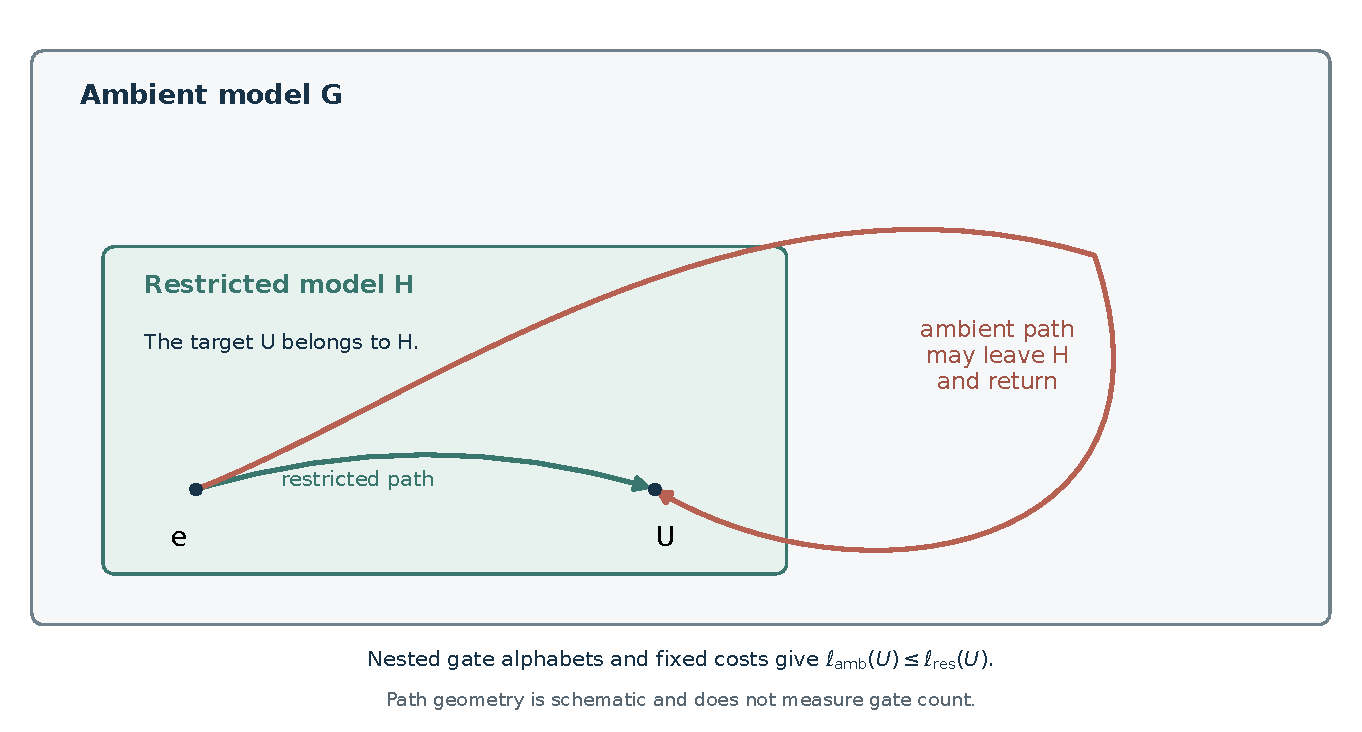
\includegraphics[width=.90\textwidth]{assets/g_gate_hierarchy.pdf}
\caption{A restricted model inside an ambient model. The target lies in the restricted class, while an ambient implementation may leave it temporarily and return. Each gate family requires its own specified inclusion and costs.}
\label{g:fig:gate-hierarchy}
\end{figure}

\subsection{Exact gate models}
\begin{definition}[Gate model]
An \emph{exact gate model} is a tuple
\[
\mathfrak M=(\mathcal X,\mathcal S,c,\circ),
\]
where $\mathcal X$ is a set of states or morphisms, $\mathcal S$ is a specified family of elementary generators, $c:\mathcal S\to\R_{\ge0}$ is a cost function, and $\circ$ is the composition law.  A word
\[
w=s_L\cdots s_1
\]
has cost
\[
c(w)=\sum_{j=1}^L c(s_j).
\]
For a target $U\in\mathcal X$, the exact synthesis cost is
\[
\ell_{\mathfrak M}(U)=\inf\{c(w):w=U\}.
\]
The value is $+\infty$ when the target has no realization.
\end{definition}

The composition law may be group multiplication, composition of permutations, composition of quantum channels, tensor-network contraction, or composition in a dagger symmetric monoidal category.  The additive cost may count all gates, only entangling gates, only non-Clifford gates, weighted error, or a vector of several resources.  Depth fits this additive model by taking admissible parallel layers as generators, rather than charging one unit to each individual gate.

\begin{definition}[Nested realization pair]
A \emph{nested realization pair} consists of restricted and ambient models
\[
\mathfrak M_{\mathrm{res}}\subseteq\mathfrak M_{\mathrm{amb}}
\]
with a common target class $\mathcal T$ of finite ambient cost and the same cost on common generators.  For $U\in\mathcal T$, define
\[
\ellRes(U)=\ell_{\mathfrak M_{\mathrm{res}}}(U),
\qquad
\ellAmb(U)=\ell_{\mathfrak M_{\mathrm{amb}}}(U).
\]
The additive defect is
\[
\Delta(U)=\ellRes(U)-\ellAmb(U).
\]
\end{definition}

When both costs are finite, $\Delta(U)$ is a metric or optimization defect.  If $\ellRes(U)=+\infty$ and $\ellAmb(U)<+\infty$, it is an existence defect.  This convention unifies finite gate savings with the failure of a restricted realization category.

\begin{proposition}[Monotonicity]
For every target in the common domain,
\[
\ellAmb(U)\le \ellRes(U).
\]
Consequently $\Delta(U)\ge0$ whenever both models use the same nonnegative cost on their common generators.
\end{proposition}
\begin{proof}
Every restricted word is also an ambient word.
\end{proof}

\subsection{Cost models are part of the theorem}
A gate-set comparison is incomplete until the cost convention is fixed.  The same pair of groups can display a defect under entangling count and no defect under total primitive count.  A SWAP gate may be primitive, may cost three CNOTs, or may be implemented by physical motion.  A local Clifford may be free in a fault-tolerant resource estimate and nonfree in a pulse-level model.

\begin{definition}[Resource vector]
Let
\[
\mathbf c(s)=(c_1(s),\ldots,c_r(s))\in\R_{\ge0}^r
\]
be the resource vector of a gate.  The achievable resource region of a target is
\[
\mathcal P_{\mathfrak M}(U)
=
\left\{
\sum_{j=1}^L\mathbf c(s_j):s_L\cdots s_1=U
\right\}.
\]
Its nondominated points form the Pareto boundary.
\end{definition}

For a weight vector $\lambda\in\R_{\ge0}^r$, scalarization gives
\[
\ell_{\mathfrak M}^{\lambda}(U)
=
\inf_{x\in\mathcal P_{\mathfrak M}(U)}\lambda\cdot x.
\]
The scalar defect $\Delta^\lambda(U)$ can vary with $\lambda$ even when the target and gate alphabets are fixed.

\begin{figure}[ht]
\centering
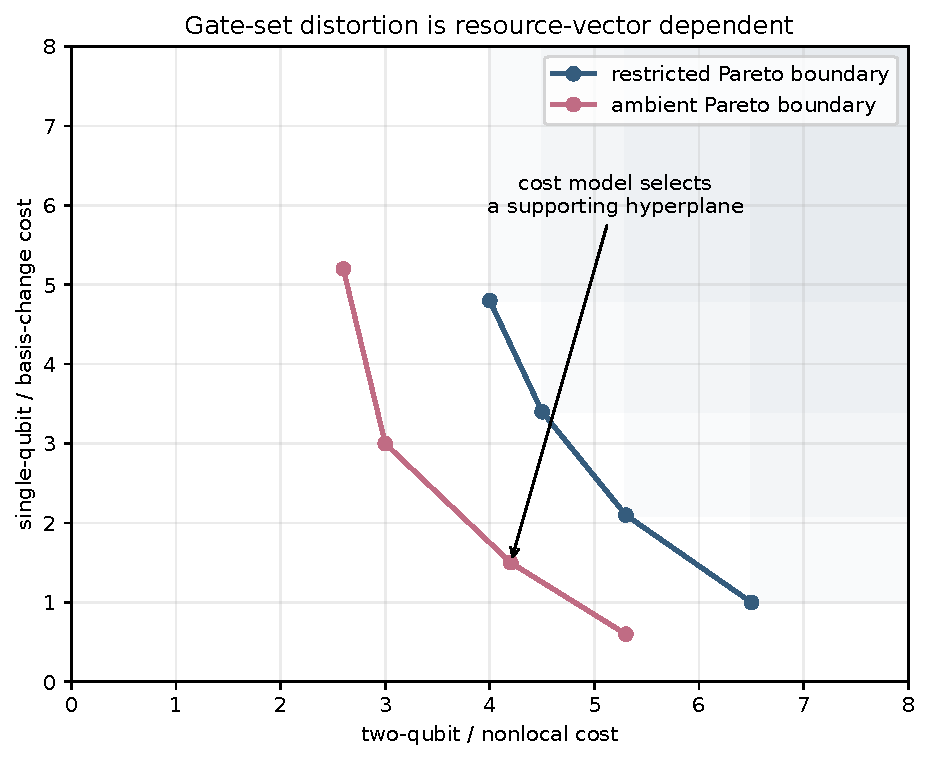
\includegraphics[width=.74\textwidth]{assets/g_resource_pareto.pdf}
\caption{Restricted and ambient Pareto regions can differ without one model dominating by the same amount under every resource weighting.}
\label{g:fig:pareto}
\end{figure}

\begin{principle}[Model specificity]
Every claimed shortcut must state the target class, elementary gate alphabet, ancilla convention, exact or approximate synthesis criterion, and cost vector.  Changing any one of these may remove, create, or reverse a defect.
\end{principle}

\subsection{Ancilla and restoration conventions}
Temporary workspace is meaningful only after its restoration rule is specified.
\begin{definition}[Ancilla conventions]
An ancilla is
\begin{enumerate}
\item \emph{clean} if it begins in a specified state and must return to that state,
\item \emph{borrowed} or \emph{dirty} if its initial state is arbitrary but must be restored,
\item \emph{consumable} if restoration is not required,
\item \emph{catalytic} if it is restored while enabling a cheaper realization of the target.
\end{enumerate}
\end{definition}
The present theory focuses on restoration.  If an auxiliary resource may be discarded, the comparison becomes a different channel or isometry synthesis problem.

\subsection{Worst-case and threshold functions}
For a size parameter $n$, let $\mathcal T_n$ denote the target family.
\begin{definition}[Extremal distortion]
Define
\[
D_n=\sup_{U\in\mathcal T_n}\Delta(U)
\]
and, when $0<\ellAmb(U)<\infty$,
\[
R_n=\sup_{U\in\mathcal T_n}
\frac{\ellRes(U)}{\ellAmb(U)}.
\]
The first defective size is
\[
\tau=\min\{n:D_n>0\}.
\]
We set a threshold to $+\infty$ when its defining set is empty.
\end{definition}

Several threshold notions should not be conflated:
\begin{align*}
\tau_{\mathrm{metric}}&=\min\{n:\exists U,\ 0<\Delta(U)<\infty\},\\
\tau_{\mathrm{exist}}&=\min\{n:\exists U,\ \ellRes(U)=\infty,\ \ellAmb(U)<\infty\},\\
\tau_{q}&=\min\{n:\exists U,\ \ell_{\le q}(U)<\ell_{\le0}(U)\},
\end{align*}
where $\ell_{\le q}$ permits at most $q$ ambient-only gates.  A model may have an early metric threshold and a later existence threshold, or no threshold at all.

\subsection{Equivalence, orbits, and classification}
A finite census should be quotiented by transformations preserving both gate models and the cost.  Depending on the problem, these may include wire permutations, local Clifford conjugation, isotopy, simultaneous row and column relabeling, or graph automorphisms.

\begin{definition}[Cost-preserving equivalence]
Targets $U$ and $V$ are equivalent if an automorphism $\varphi$ of the ambient realization system satisfies
\[
\varphi(U)=V,
\qquad
\varphi(\mathcal S_{\mathrm{res}})=\mathcal S_{\mathrm{res}},
\qquad
\varphi(\mathcal S_{\mathrm{amb}})=\mathcal S_{\mathrm{amb}},
\]
and preserves the gate costs.
\end{definition}
Under this equivalence, both lengths and the defect are orbit invariants.  A useful threshold theorem should classify minimal defective orbits, not merely list raw matrices.

\subsection{Approximate synthesis and border defects}
For continuous gate models, exact word length can differ from the minimum length achievable as a limit.
\begin{definition}[Border cost]
Let $\overline{\mathcal W}_{L}$ be the topological or Zariski closure of targets realizable with cost at most $L$.  The border cost is
\[
\underline\ell(U)=\inf\{L:U\in\overline{\mathcal W}_{L}\}.
\]
The border defect is
\[
\underline\Delta(U)=
\underline\ell_{\mathrm{res}}(U)-
\underline\ell_{\mathrm{amb}}(U).
\]
\end{definition}
This is the circuit analogue of the distinction between tensor rank and border rank.  An exact defect can disappear under degeneration, persist, or become larger after approximation changes the relevant cost geometry.

\subsection{Metric and existence defects in one category}
Let $\mathcal C_{\mathrm{res}}\subseteq\mathcal C_{\mathrm{amb}}$ be categories with weighted generating morphisms.  For a morphism $f$ in the restricted target class, the same definition
\[
\Delta(f)=c_{\mathrm{res}}(f)-c_{\mathrm{amb}}(f)
\]
includes group-word metrics, adaptive quantum channels, tensor-network realizations, and orthogonality designs.  This categorical form is essential when the ambient model permits measurement, branching, postselection, or entangled objects that do not lie in a common group.

\begin{boundarybox}
The abstract definition does not prove that a defect exists.  It provides a common language in which a finite search, a symbolic identity, and a lower-bound certificate can be compared without changing the meaning of the target or the cost.
\end{boundarybox}

\subsection{A standard theorem package}
A mature gate-set distortion result should contain as many of the following components as the model allows:
\begin{enumerate}
\item a precisely defined nested gate pair and cost vector,
\item a smallest defective target or a no-defect theorem below a threshold,
\item an explicit ambient word,
\item a restricted lower-bound certificate,
\item classification modulo cost-preserving equivalence,
\item a reusable catalytic normal form,
\item direct-sum, recursive, or tensor amplification,
\item generic-rigidity or sparsity results,
\item a certificate-producing implementation,
\item a clear account of which statements are symbolic, computed, or conjectural.
\end{enumerate}
The remainder of the monograph follows this package.

\section{Catalytic holonomy, excursion geometry, and resource reuse}\label{g:ch:holonomy}
\index{holonomy}
\index{Schreier graph}
\index{catalytic conjugation}
\index{dirty workspace}
\index{resource amortization}


\subsection{Subgroup metrics and Schreier loops}
Assume first that the restricted and ambient models are groups
\[
H=\langle\mathcal S_H\rangle
\le
G=\langle\mathcal S_G\rangle.
\]
For $h\in H$, the intrinsic and ambient word metrics are
\[
\ell_H(h)=|h|_{\mathcal S_H},
\qquad
\ell_G(h)=|h|_{\mathcal S_G}.
\]
In the group-metric statements, the generating alphabets are symmetric and a generator and its inverse have equal cost.  The quotient geometry is the left Schreier graph $G/H$, with edges $gH\longmapsto sgH$.  For the base-fiber assertion below, assume also $\mathcal S_H=\mathcal S_G\cap H$.  This last condition excludes additional ambient primitives that already lie in $H$ but have no equally cheap restricted realization.

\begin{theorem}[Holonomy-compression identity]
Let every generator have unit cost.  For $h\in H$, $\ell_G(h)$ is the minimum length of a based loop in $G/H$ whose lifted word has holonomy $h$.  The intrinsic length $\ell_H(h)$ is the minimum length among loops that remain in the base fiber.
\end{theorem}
\begin{proof}
An ambient word $s_k\cdots s_1=h$ projects to the loop
\[
H,
s_1H,
s_2s_1H,
\ldots,
hH=H.
\]
Conversely, a based Schreier loop has product in $H$.  If every prefix lies in $H$, each edge label is the product of two elements of $H$ and belongs to $\mathcal S_G\cap H=\mathcal S_H$.  Conversely every restricted word remains in the base fiber.  Minimizing the labeled words with endpoint $h$ gives the two asserted lengths.
\end{proof}

Thus
\[
\Delta_{H\hookrightarrow G}(h)
=
\text{intrinsic fiber cost}
-
\text{shortest holonomy loop cost}.
\]
This is the geometric content of a dirty-workspace shortcut.

\begin{figure}[ht]
\centering
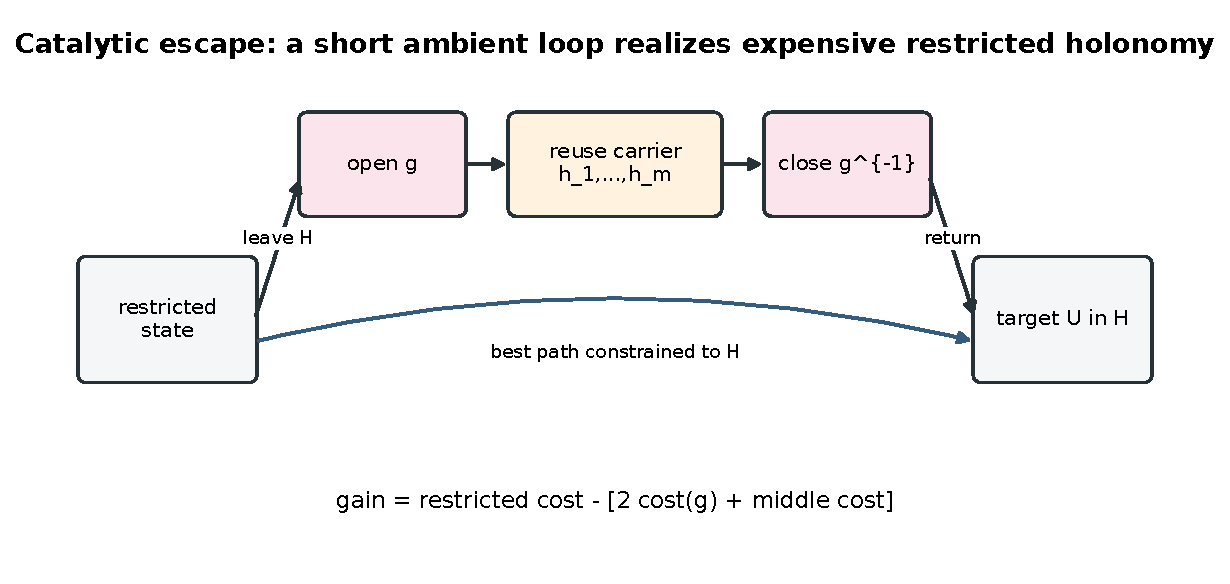
\includegraphics[width=.90\textwidth]{assets/g_catalytic_excursion_general.pdf}
\caption{A catalytic excursion leaves a restricted fiber, reuses an ambient state, and returns with nontrivial holonomy.}
\label{g:fig:catalytic-excursion}
\end{figure}

\subsection{The basic conjugation inequality}
Let $g\in G$ and $k\in H$ satisfy $gkg^{-1}\in H$.  Then
\[
\ell_G(gkg^{-1})
\le 2\ell_G(g)+\ell_H(k).
\]
Define the intrinsic conjugation stretch
\[
\operatorname{Stretch}_g(k)
=
\ell_H(gkg^{-1})-\ell_H(k).
\]

\begin{proposition}[Catalytic stretch criterion]
If
\[
\operatorname{Stretch}_g(k)>2\ell_G(g),
\]
then $gkg^{-1}$ has positive defect.
\end{proposition}
The opening and closing cost is paid once.  Every useful consumer inside the excursion contributes to the stretch.

\subsection{Many consumers and catalytic excess}
Suppose the middle word is
\[
k=h_m\cdots h_1,
\qquad h_i\in H.
\]
The ambient word
\[
gh_m\cdots h_1g^{-1}
\]
has cost at most
\[
2c(g)+\sum_i c(h_i).
\]
If the restricted images $gh_ig^{-1}$ require costs $r_i$ and a lower-bound invariant proves that their obligations cannot be shared, then
\[
\ell_H(gkg^{-1})\ge\sum_i r_i.
\]
A sufficient inequality is
\[
\sum_i(r_i-c(h_i))>2c(g).
\]
The left side is the gross catalytic benefit.  The right side is the restoration cost.

\begin{definition}[Catalytic excess]
For a normal form with $r$ matched excursions and $C$ useful cross interactions, define
\[
\mathcal E=C-2r
\]
when each consumer contributes one unit and each opening or closing costs one unit.
\end{definition}
Positive excess is necessary in the simplest transvection model, but it is not sufficient.  An all-cross configuration may admit a mirror word of equal restricted length.  Temporal asymmetry or phase holonomy is also required.

\subsection{Excursion budgets}
Counting ambient-only gates is only one measure of how far a circuit leaves its restricted model.
\begin{definition}[Excursion profile]
For a circuit path $X_0,X_1,\ldots,X_L$, an excursion profile may include
\begin{enumerate}
\item the number $q$ of ambient-only gates,
\item the maximum Schreier distance $d(X_tH,H)$,
\item the rank of a forbidden block,
\item the bandwidth of a forbidden dependency,
\item the number of simultaneously open catalytic intervals,
\item the intersection graph of those intervals,
\item the maximum algebraic degree created temporarily,
\item the maximum ancilla dimension or branch count.
\end{enumerate}
\end{definition}
The established linear family shows that a rank-one, bandwidth-one excursion using exactly two forbidden gates can save linearly many operations.  Thus geometric excursion size need not control computational benefit.

\subsection{Catalytic interval geometry}
Associate to every matched opening and closing operation an interval
\[
I_j=[t_j^{\mathrm{open}},t_j^{\mathrm{close}}].
\]
The family of intervals can be disjoint, nested, laminar, or crossing.

\begin{principle}[First higher-order frontier]
Independent or disjoint intervals often reduce to additive copies of a one-catalyst analysis.  Crossing intervals are the first place where one dirty resource can alter another and where a multiplicative distortion larger than the clean one-carrier value may occur.
\end{principle}

Define the catalytic width
\[
w_{\mathrm{cat}}=
\max_t
\#\{j:t\in I_j\}.
\]
One may then study
\[
D_n^{(w)}
=
\max_{U}
\left(
\ellRes(U)-\ellAmb^{(w)}(U)
\right),
\]
where the ambient circuit has width at most $w$.  The unitriangular snapshot family gives $D_n^{(1)}=\Omega(n)$ in its corresponding interval model.

\subsection{Four recurrent catalytic mechanisms}
\subsubsection{Basis-change catalysis}
An ambient gate $g$ changes the frame in which several restricted operations are cheap:
\[
h_i\mapsto gh_ig^{-1}.
\]
Hadamard and Fourier transforms are the basic quantum examples.  The frame is restored at the end.

\subsubsection{Commutator catalysis}
An ambient commutator creates a new direction:
\[
[g,h]=ghg^{-1}h^{-1}.
\]
For continuous controls,
\[
e^{\varepsilon X}e^{\varepsilon Y}e^{-\varepsilon X}e^{-\varepsilon Y}
=
e^{\varepsilon^2[X,Y]+O(\varepsilon^3)}.
\]
The desired effective generator may lie in the restricted algebra even though the path does not.

\subsubsection{Degree catalysis}
A Toffoli, CCZ, or non-Gaussian gate can create higher algebraic degree or higher moments temporarily.  If the nonlinear object is reused and canceled, the final target may remain affine, diagonal, or Gaussian.

\subsubsection{Branch and workspace catalysis}
Ancillas, measurements, reset, teleportation, and classical feedforward enlarge the realization category.  The resource is a temporary branch, subsystem, or borrowed state rather than a group element.

\subsection{When defects are impossible}
A useful positive theorem is a criterion guaranteeing geodesic convexity.
\begin{proposition}[One-Lipschitz retraction criterion]
Suppose there is a group homomorphism $\pi:G\to H$ with $\pi|_H=\operatorname{id}_H$ such that every ambient generator $s\in\mathcal S_G$ satisfies
\[
\ell_H(\pi(s))\le c(s).
\]
Then
\[
\ell_H(h)\le\ell_G(h)
\]
for every $h\in H$, hence the two metrics agree on $H$.
\end{proposition}
\begin{proof}
For an ambient word $h=s_L\cdots s_1$, multiplicativity gives $h=\pi(h)=\pi(s_L)\cdots\pi(s_1)$.  Subadditivity and the generator bounds give $\ell_H(h)\le\sum_j c(s_j)$.  Taking the infimum over ambient words proves the claim.
\end{proof}

The unitriangular counterexample proves that no such generator-wise one-Lipschitz retraction exists for the lower transvection model inside the all-transvection model.

\subsection{Weighted restoration and phase transitions}
Let every restricted gate cost one and every ambient-only gate cost $\lambda$.  For a catalyst used by $v$ consumers with unit benefit, the displayed construction has net gain at least
\[
v-2\lambda.
\]
The critical weight is therefore target and mechanism dependent.

\begin{definition}[Critical catalyst penalty]
For a target family $U_n$, define
\[
\lambda_c(U_n)
=
\sup\{\lambda:\ell_{\lambda,\mathrm{amb}}(U_n)<\ellRes(U_n)\}.
\]
\end{definition}
Determining $\lambda_c$ exactly is a refined synthesis problem.  It can be more physically meaningful than unweighted gate count.

\subsection{Restoration is the source of nontriviality}
If the ambient resource need not be restored, the opening cost can dominate the comparison and many examples become trivial.  Catalytic escape is strongest when the following all hold:
\begin{enumerate}
\item the final target lies entirely in the restricted class,
\item every auxiliary subsystem or violated constraint is restored,
\item the ambient-only resource is used more than once,
\item the restricted lower bound charges the same repeated obligations separately,
\item the gain survives a realistic weighted cost.
\end{enumerate}

\begin{conjecturebox}
In many finite gate hierarchies, minimal defects should admit a bounded-width catalytic normal form.  Proving or refuting this would turn an unrestricted synthesis search into a search over a finite family of excursion motifs.
\end{conjecturebox}

\section{First arrival, spectral packets, algebraic rarity, and tensor regularization}\label{g:ch:spectral-algebraic}
\index{Green kernel}
\index{first-arrival valuation}
\index{word map}
\index{algebraic defect locus}
\index{border rank}
\index{tensor capacity}


\subsection{Word distance as first arrival}
Let $G$ be finite and let $S=S^{-1}$ be a symmetric generating multiset.  In the right regular representation, define
\[
A_S=\sum_{s\in S}\rho(s).
\]
Then
\[
\langle\delta_g,A_S^k\delta_e\rangle
\]
counts length-$k$ words ending at $g$.

\begin{theorem}[Endpoint Green valuation]
The word distance is
\[
d_S(e,g)
=
\ord_{z=0}
\left\langle
\delta_g,(I-zA_S)^{-1}\delta_e
\right\rangle.
\]
\end{theorem}
\begin{proof}
Expand the resolvent as a formal power series:
\[
(I-zA_S)^{-1}=\sum_{k\ge0}z^kA_S^k.
\]
The first nonzero endpoint coefficient occurs at the shortest word length.
\end{proof}

For strictly positive integer costs, replace each generator $s$ by the monomial $z^{c(s)}\rho(s)$.  Every coefficient then counts finitely many words of a given total cost, and the same formal inverse is defined.  Zero-cost cycles require separate treatment: they can create infinitely many words of cost zero, so the ordinary counting series need not exist.  The finite atlases with free gates use shortest-path search with zero-cost edges instead.  Multivariate variables can track several resources when the grading gives every generator positive total degree.

\subsection{Why eigenvalues alone are insufficient}
If
\[
A_S=\sum_\lambda\lambda\Pi_\lambda,
\]
then
\[
\mathcal G_{S,g}(z)
=
\sum_\lambda
\frac{\langle\delta_g,\Pi_\lambda\delta_e\rangle}{1-\lambda z}.
\]
The eigenvalues and multiplicities do not determine the endpoint coefficients
\[
\langle\delta_g,\Pi_\lambda\delta_e\rangle.
\]
Two Cayley or Schreier systems can therefore be cospectral and still have different first-arrival behavior at distinguished targets.

\begin{principle}[Embedded packet principle]
For threshold questions, a spectral label is usually weaker than an embedded spectral projector.  The matrix coefficients of the projector relative to the initial and target states retain positional information that multiplicities erase.
\end{principle}

This distinction recurs in the Latin-square example discussed later.  The natural commuting row, column, and symbol operators have universal eigenvalue packets at fixed order, while the embedded incidence and transition data still vary.

\subsection{Subgroup-holonomy Fourier packets}
Let $H\le G$.  Let $\mu_k(h)$ count ambient words of length $k$ with product $h\in H$.  For every irreducible representation $\tau\in\widehat H$, define
\[
\widehat\mu_k(\tau)
=
\sum_{h\in H}\mu_k(h)\tau(h).
\]
Fourier inversion gives
\[
\mu_k(h)
=
\frac1{|H|}
\sum_{\tau\in\widehat H}
\dim(\tau)
\operatorname{tr}
\bigl(
\tau(h^{-1})\widehat\mu_k(\tau)
\bigr).
\]
The matrix-valued Green packet
\[
\widehat{\mathcal G}_\tau(z)
=
\sum_{k\ge0}\widehat\mu_k(\tau)z^k
\]
recovers every endpoint series after Fourier inversion.

The trivial representation records only the total number of loops returning to the subgroup.  Nontrivial $H$-types retain their holonomy.  This yields a hierarchy:
\[
\text{spherical return data}
\prec
\text{type-resolved holonomy packets}
\prec
\text{exact endpoint realization}.
\]

\subsection{Word maps and product loci}
Let $K$ be a field and let $X\subseteq G$ be an algebraic gate family.  For a fixed length $L$, multiplication defines
\[
\mu_L:X^L\to G,
\qquad
(x_L,\ldots,x_1)\mapsto x_L\cdots x_1.
\]
The exact length-$L$ locus is $\mu_L(X^L)$, and the length-at-most-$L$ locus is a finite union of such images when the gate family has finitely many components.

\begin{theorem}[Dimension per gate]
Suppose every irreducible component of $X$ has dimension at most $r$.  Then the Zariski closure of the locus reachable in at most $L$ gates has dimension at most $rL$.
\end{theorem}
\begin{proof}
Every component of $X^L$ has dimension at most $rL$.  A morphism cannot increase dimension.  A finite union has dimension equal to the maximum dimension of its components.
\end{proof}

For scaled transvections, $r=1$.  This immediately yields generic lower bounds in a target variety whose dimension exceeds $L$.

\subsection{Generic rigidity}
Work over an algebraically closed field.  Suppose the restricted target variety $V$ is irreducible of dimension $N$, every target has a restricted realization using at most $N$ unit-cost gates, and the ambient alphabet is an algebraic family with finitely many components of dimension at most one.  Then ambient realizations of length below $N$ occupy a proper closed subset of $V$.

\begin{theorem}[Abstract generic rigidity]
Under the preceding hypotheses, there is a nonempty Zariski-open subset $\Omega\subseteq V$ such that
\[
\ellRes(U)=\ellAmb(U)=N
\qquad(U\in\Omega).
\]
\end{theorem}
The unitriangular theorem in the core chapter is a concrete instance with
\[
N=\binom n2.
\]

\subsection{Defect codimension}
If every target has restricted cost at most $N$, then defect at least $d$ forces ambient cost at most $N-d$.  The dimension-per-gate theorem gives
\[
\codim_V\overline{\{U:\Delta(U)\ge d\}}
\ge d
\]
when each ambient gate carries one parameter.

\begin{principle}[Rare but amplifiable]
At fixed dimension, large defects require increasingly special algebraic conditions.  Under direct sums, recursive lifts, or tensor products, a point on a thin exceptional stratum can nevertheless seed a macroscopic family.
\end{principle}

This is one of the central tensions of the subject.  Catalysis is neither generic nor negligible.

\subsection{Finite-field sparsity}
A word-counting analogue applies over $\F_q$.  If the ambient alphabet has at most $M(q-1)$ nontrivial scaled gates, then the number of targets reached in $L$ gates is at most
\[
\sum_{j=0}^L[M(q-1)]^j.
\]
When the target space has $q^N$ points and defect $d$ implies ambient length at most $N-d$, the crude bound is
\[
\Prob[\Delta\ge d]
=O_{N,M}(q^{-d}).
\]
The estimate can be sharpened by orbit counting, stabilizers, and the geometry of word-map fibers.

\subsection{Direct sums and monoidal amplification}
Suppose targets admit a direct sum $U\oplus V$ and a homomorphism from the large restricted group onto the two factor groups sends $U\oplus V$ to $(U,V)$.  Require the aggregate generator bound
\[
\ellRes(\pi_1(s))+\ellRes(\pi_2(s))\le c(s)
\]
for every large restricted generator $s$.  Assume that both restricted and ambient factor circuits embed into the corresponding large model without increasing cost.  Then
\[
\ellRes(U\oplus V)
=
\ellRes(U)+\ellRes(V).
\]
Indeed, projecting any word and summing the two factor bounds gives the lower bound, while concatenating the embedded factor circuits gives the upper bound.  Separate one-Lipschitz projections alone do not imply this sum inequality.
Under the ambient embedding assumption, the constructive upper bound is
\[
\ellAmb(U\oplus V)
\le
\ellAmb(U)+\ellAmb(V),
\]
so
\[
\Delta(U\oplus V)
\ge
\Delta(U)+\Delta(V).
\]
One finite defect therefore gives an unbounded additive family.

\subsection{Tensor products and normalized rates}
Let $U$ have dimension $m$ and $V$ dimension $n$.  In linear transvection models with tree-tight certificates,
\[
\ellRes(U\otimes V)
=
n\ellRes(U)+m\ellRes(V).
\]
The ambient model satisfies the corresponding inequality.  Normalizing by dimension gives an entropy-like law:
\[
\frac{\ellRes(U\otimes V)}{mn}
=
\frac{\ellRes(U)}m+
\frac{\ellRes(V)}n.
\]
The normalized defect is superadditive under tensor products.

\begin{definition}[Tensor synergy]
Define
\[
\Syn(U,V)
=
n\ellAmb(U)+m\ellAmb(V)-\ellAmb(U\otimes V).
\]
Positive synergy means that the joint ambient realization improves on independent lifted circuits.
\end{definition}
Restricted tree-tight metrics have zero tensor synergy.  Ambient synergy is a possible source of collective activation.

\begin{definition}[Stable tensor cost]
For a size-$m$ target $U$, define
\[
\tau_\otimes(U)
=
\lim_{r\to\infty}
\frac{\ellAmb(U^{\otimes r})}{r m^{r-1}},
\]
when the subadditivity argument applies.  Define
\[
\kappa_\otimes(U)
=
\ellRes(U)-\tau_\otimes(U).
\]
\end{definition}
Fekete's lemma gives the limit from the tensor subadditivity inequality.

\begin{figure}[ht]
\centering
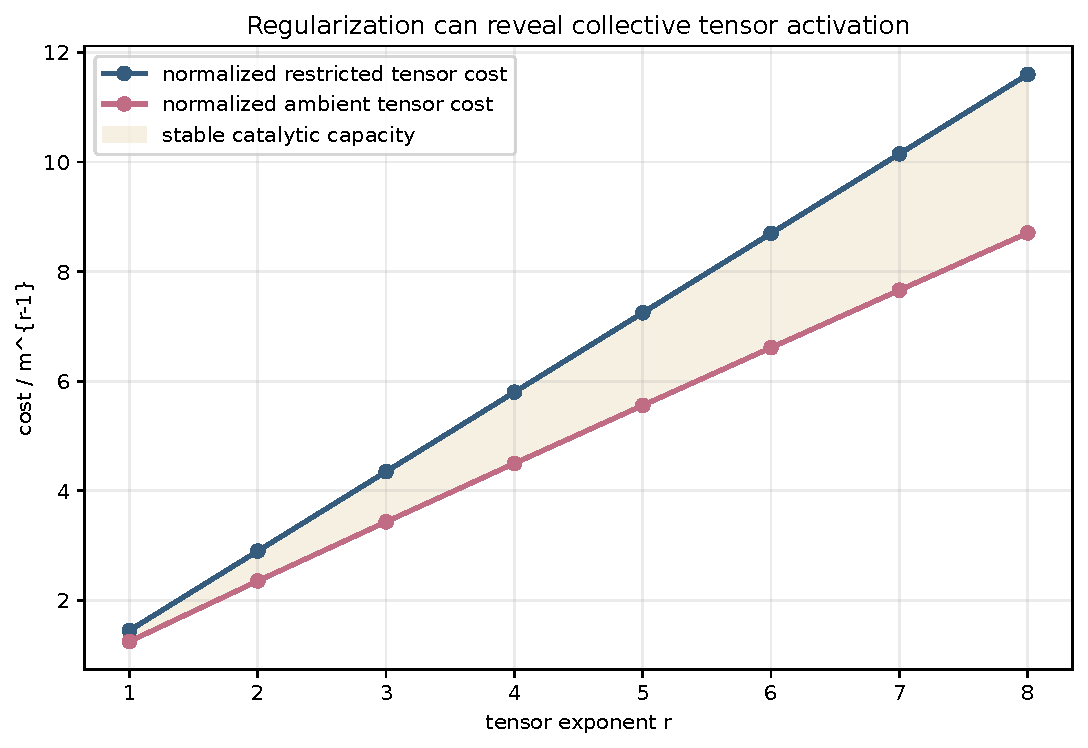
\includegraphics[width=.72\textwidth]{assets/g_tensor_capacity.pdf}
\caption{Schematic stable tensor capacity.  The figure illustrates definitions, not measured data.}
\end{figure}

\begin{definition}[Tensor activation]
A target is tensor activated if
\[
\Delta(U)=0
\quad\text{but}\quad
\kappa_\otimes(U)>0.
\]
\end{definition}
This is analogous to regularized capacities and asymptotic ranks.  It asks whether collective synthesis can unlock a catalyst invisible in one copy.

\subsection{Border catalysis}
Let $X_{\mathrm{res}}$ and $X_{\mathrm{amb}}$ be algebraic gate varieties.  The exact product rank is
\[
\operatorname{rk}_{X}(U)
=
\min\{L:U\in X^L\},
\]
while border product rank is
\[
\underline{\operatorname{rk}}_{X}(U)
=
\min\{L:U\in\overline{X^L}\}.
\]
The four possible comparisons are:
\begin{enumerate}
\item exact and border defects both positive,
\item exact defect positive but border defect zero,
\item one-copy defect zero but tensor-regularized defect positive,
\item ambient and restricted border ranks both smaller than exact ranks but by different amounts.
\end{enumerate}
Each requires a separate certificate.  Numerical approximation alone does not distinguish them.

\subsection{A packet-resolved threshold principle}
Combining the preceding constructions gives the following architecture.
\begin{enumerate}
\item A coarse commutative algebra supplies spherical spectral packets.
\item Embedded projectors retain incidence and endpoint position.
\item Noncommutative transition data record holonomy.
\item A realization theorem decides whether the packet has a restricted representative and at what cost.
\item Direct sums and tensor products propagate local defects.
\end{enumerate}

\begin{figure}[ht]
\centering
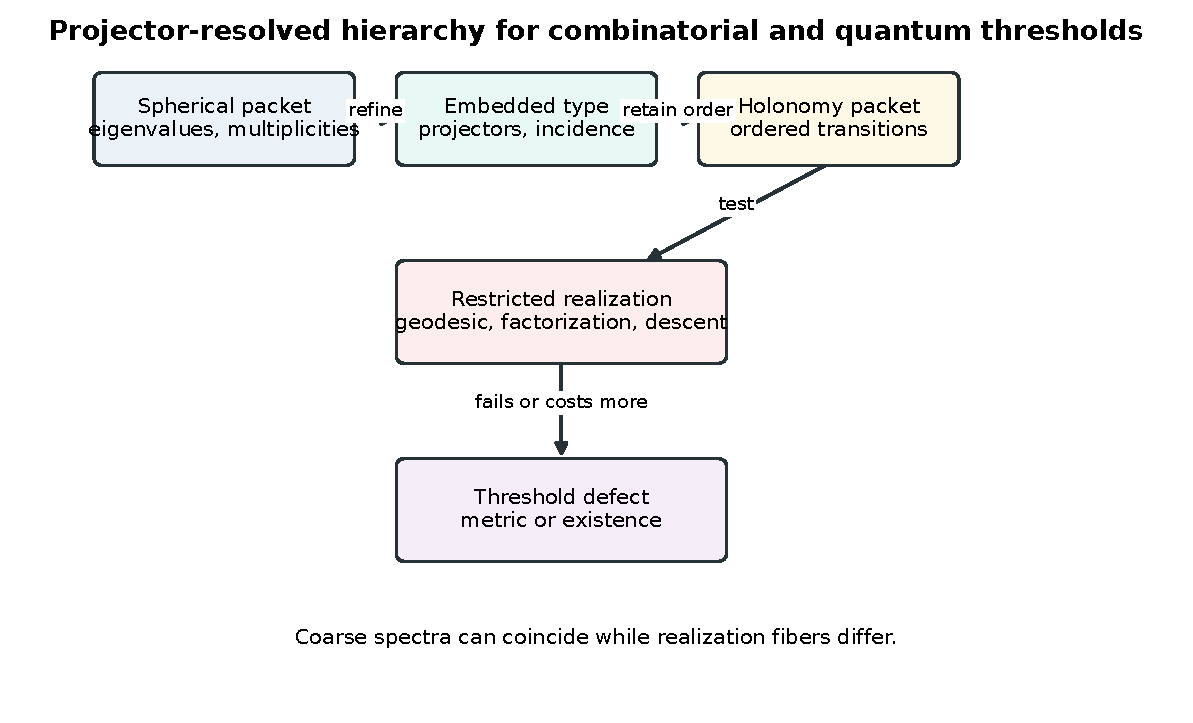
\includegraphics[width=.86\textwidth]{assets/g_packet_hierarchy.pdf}
\caption{The spectral-to-realization hierarchy.}
\label{g:fig:packet-hierarchy}
\end{figure}

\begin{boundarybox}
A packet hierarchy organizes evidence.  It does not replace the final lower bound, positivity argument, orthogonality construction, or descent theorem.  Classification and realization remain distinct layers.
\end{boundarybox}

\section{Matroidal state geometry, quiver factorizations, and root-system catalysis}\label{g:ch:matroid-quiver-roots}
\index{matroid}
\index{quiver}
\index{root system}
\index{Chevalley commutator}
\index{pattern group}


\subsection{Intermediate states as a representable matroid}
A linear circuit visits vectors that satisfy exact dependence relations.  If $\mathcal V$ is the set of all row states appearing during a computation, then $\mathcal V$ determines a representable matroid.  A transvection
\[
u\longmapsto u+a v
\]
creates a three-point projective line
\[
[u],\ [v],\ [u+av].
\]
The ambient circuit chooses a tour through this projective configuration.  A flag-preserving circuit must lift the same dependencies through prescribed pivot positions.

\begin{definition}[Flagged matroid tour]
Let $M$ be a representable matroid with designated initial basis, target basis, and consumer states.  A \emph{flagged tour} is a sequence of basis exchanges or transvections in which the $i$th carrier remains inside a specified filtration layer.  An ambient tour drops this constraint.
\end{definition}
The six-row atom realizes the graphic regular matroid $M(K_4)$.  Its ambient state tour is shorter than every compatible flag lift.  Regularity explains why the same dependence pattern survives every field and, through integer matrices, every nonzero commutative coefficient ring in the stated model.

\subsection{Matroidal classification problem}
The first general classification problem is:
\begin{quote}
Which regular matroids admit designated carrier and consumer roles for which an ambient tour is shorter than every flag-compatible tour?
\end{quote}
Natural subclasses are graphic, cographic, and network matrices.  Potential invariants include branch width, circuit size, excluded minors, and the number of consumer incidences supported by one projective line.

\begin{conjecturebox}
Minimal field-universal catalytic atoms should be governed by regular matroids, while characteristic-dependent atoms should arise from representable matroids with excluded-characteristic minors.
\end{conjecturebox}
This conjecture is a programmatic guide.  The core paper establishes only the $M(K_4)$ instance.

\subsection{Dynamic rank-one factorization}
Consider a height-two block shear
\[
E(C)=
\begin{pmatrix}
I_s&0\\
C&I_t
\end{pmatrix}.
\]
A restricted circuit may change source and output bases while transmitting rank-one terms.  Let $P_r\in U_s$ be the source basis before the $r$th transmission and let $Q_{>r}\in U_t$ be the future output basis.  A cross gate contributes
\[
Q_{>r}e_{i_r}e_{j_r}^{T}P_{<r}
\]
to the final block.  Hence
\[
C=
\sum_{r=1}^{c}
Q_{>r}e_{i_r}e_{j_r}^{T}P_{<r},
\]
with closed basis paths
\[
P_{\mathrm{final}}=I_s,
\qquad
Q_{\mathrm{final}}=I_t.
\]

\begin{definition}[Dynamic rank-one cost]
The dynamic rank-one cost of $C$ is the minimum of
\[
\text{source basis motion}
+
\text{output basis motion}
+
\text{number of transmissions}
\]
over such timed decompositions.
\end{definition}
Ordinary rank retains only the number of transmissions after arbitrary bases are given for free.  Circuit complexity charges the closed paths needed to expose and restore those bases.

\subsection{Quiver gate models}
Let $Q=(Q_0,Q_1)$ be a quiver.  Associate a vector space $V_v$ to every vertex.  Internal gates change bases inside $V_v$, while edge gates transmit low-rank maps along arrows.  A target is a representation of the path algebra or an automorphism of a filtered quiver module.

This generalization includes:
\begin{itemize}
\item block-triangular linear circuits,
\item network coding with reversible local state,
\item layered dataflow architectures,
\item incidence-algebra transformations,
\item tensor networks with reusable bond states.
\end{itemize}

A catalytic excursion can temporarily activate a forbidden arrow or enlarge a vertex space.  The restored target still lies in the original quiver representation class.

\begin{skeletonbox}
A quiver threshold theorem should specify a forbidden-arrow motif, an exact ambient word, a projection-based restricted lower bound, and an amplification operation under quiver substitution.  The unitriangular snapshot family is the linearly ordered one-dimensional-vertex case.
\end{skeletonbox}

\subsection{Pattern groups and architecture constraints}
For a poset $P$, define the pattern group
\[
U_P(K)
=
\{I+A:A_{ij}=0\text{ unless }j<_P i\}.
\]
When the allowed positions are transitively closed, $U_P$ is a group.  Compare the intrinsic metric generated by $P$-allowed transvections with the metric induced by all transvections.

The first threshold now depends on the forbidden-edge geometry of $P$.  One may ask whether a six-role catalytic motif embeds as a generator-preserving retract.  If it does, the larger architecture inherits a defect.

\begin{proposition}[Retraction inheritance]
Suppose a smaller nested pair $H\le G$ embeds into $H'\le G'$ by homomorphisms preserving the inclusion, the ambient embedding does not increase gate cost, and there is a homomorphic retraction $\pi:H'\to H$ onto the embedded copy.  Require $\ell_H(\pi(s))\le c(s)$ for every restricted generator $s$ of $H'$.  Then every defect in $H\le G$ gives a defect at least as large in $H'\le G'$.
\end{proposition}
The proof projects a restricted word in the larger system and embeds the shorter ambient word from the smaller system.

\subsection{Root subgroups and Chevalley relations}
Let $G$ be a split reductive group \cite{g:Carter1972,g:Humphreys1975} with root system $\Phi$.  Let $\Psi\subseteq\Phi$ be a closed set of allowed roots and let $U_\Psi$ be generated by the root groups $x_\beta(t)$ for $\beta\in\Psi$.  Define
\[
\ell_\Psi(u)
=
\min\{L:u=x_{\beta_L}(t_L)\cdots x_{\beta_1}(t_1),\ \beta_i\in\Psi\},
\]
and let $\ell_\Phi$ permit all roots.

The Chevalley conjugation formula has the schematic form
\[
x_\alpha(a)x_\beta(b)x_\alpha(a)^{-1}
=
x_\beta(b)
\prod_{k>0}
x_{\beta+k\alpha}(c_k a^k b).
\]
A forbidden root $\alpha$ can therefore create several allowed root effects before being removed.

\begin{figure}[ht]
\centering
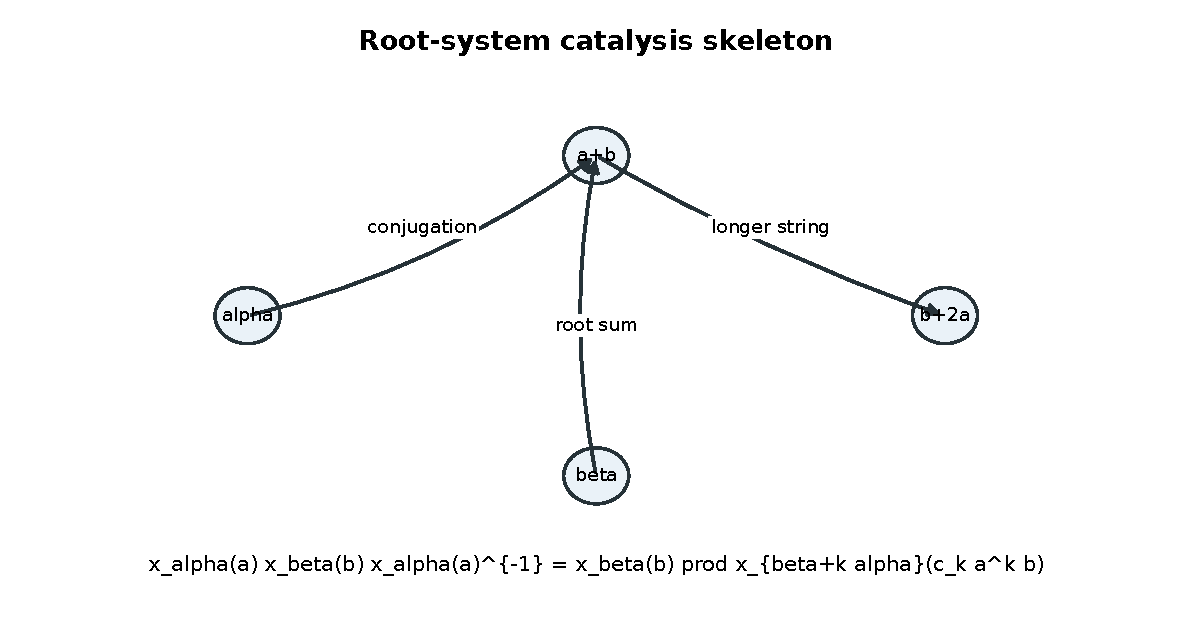
\includegraphics[width=.80\textwidth]{assets/g_root_catalysis.pdf}
\caption{A root-string template for catalytic generation.  Longer strings may support more gain per opening and closing pair.}
\end{figure}

\subsection{Type \texorpdfstring{$A$}{A} and beyond}
Row transvections are root-group elements of type $A$.  The established unitriangular atom occurs in $A_5$.  In nonsimply laced systems, root strings can have length greater than two.  This raises the possibility that one ambient root can create multiple restricted effects per consumer.

\begin{conjecture}[Long-root catalytic gain]
There exist gate alphabets in types $B$, $C$, or $G_2$ for which a clean one-catalyst multiplicative distortion exceeds the type-$A$ snapshot limit of $3/2$.
\end{conjecture}
No lower-bound certificate is presently supplied.  The conjecture identifies a concrete reason to test nonsimply laced root systems rather than merely repeating type $A$ computations.

\subsection{Symplectic root systems and Clifford logic}
The binary Clifford group modulo phases acts through $\Sp(2n,2)$.  A parabolic subgroup stabilizing a Lagrangian is the symplectic analogue of a Borel or flag-preserving circuit class.  Hadamard gates leave this parabolic, while $S$, $\CZ$, and $\CX$ preserve it.  The exact Clifford censuses in \cref{g:ch:clifford} are therefore a first root-system extension of the linear theory.

\subsection{Categorical realization defects}
The group framework does not cover measurement, feedforward, postselection, or entangled design objects.  Let
\[
\mathcal C_{\mathrm{res}}
\subseteq
\mathcal C_{\mathrm{amb}}
\]
be monoidal categories with costed generators.  A target morphism can have a finite metric defect or an infinite existence defect.

The categorical viewpoint supports:
\begin{itemize}
\item unitary versus measurement-assisted circuits,
\item product-state versus entangled realizations,
\item clean versus borrowed ancilla categories,
\item symmetry-preserving versus symmetry-breaking channels,
\item exact versus approximate completion.
\end{itemize}
The common invariant is still the cost of a restored target.  What changes is the geometry of the path and the meaning of holonomy.

\subsection{A general research dichotomy}
The broad program separates into two tasks.
\begin{enumerate}
\item \textbf{Construction:} exhibit an ambient excursion whose repeated consumers produce a cheaper target.
\item \textbf{Certification:} prove that the restricted category cannot share the same obligations as efficiently.
\end{enumerate}
Conjugation identities often solve the first task.  The second is the difficult part and requires model-specific invariants such as interval-tree rank, symplectic flag length, algebraic degree, phase-polynomial rank, covariance constraints, or branch complexity.

\chapter{The complete linear core}
\section{Introduction}

A CNOT circuit on $n$ labeled wires represents an element of $\GL_n(\F_2)=\SL_n(\F_2)$, and minimizing its gate count is the word-metric problem for transvection generators.  This formulation supports asymptotically efficient synthesis, architecture-aware elimination, computable lower bounds, and exact small-width optimization \cite{g:SaeediMarkov2013,g:PatelMarkovHayes2008,g:JiangEtAl2020,g:GoubaultEtAl2021,g:Bataille2022,g:BuFanJoo2025,g:ChristensenEtAl2025,g:WebsterEtAl2025}.  Recent work has also produced stronger explicit lower-bound families and established NP-completeness of exact all-to-all CNOT distance \cite{g:Jorgensen2026,g:GongYu2026,g:AcuavivaEtAl2026}.  The present paper studies a different comparison: the target is lower unitriangular, but the circuit is either required to respect that ordered structure or allowed to leave it temporarily.

Let $R$ be a nonzero commutative ring with identity.  A row transvection is
\[
\tau_{t,s}(a)=I+aE_{t,s},
\qquad t\ne s,
\qquad a\in R\setminus\{0\},
\]
acting by
\[
R_t\longleftarrow R_t+aR_s.
\]
The transvection is \emph{lower directed} when $s<t$.  The lower-directed gates generate $\U_n(R)$.  We compare
\[
\ellDown(A)
 =\min\{\text{number of lower-directed transvections producing }A\}
\]
with
\[
\ellAll(A)
 =\min\{\text{number of arbitrary row transvections producing }A\},
\qquad A\in\U_n(R).
\]
For a field $\F$, the first metric is intrinsic to the unipotent radical and the second is induced from the elementary group $\Egrp_n(\F)=\SL_n(\F)$.

The equality $\ellDown(A)=\ellAll(A)$ is tempting because the target and the obvious Gaussian-elimination paths are lower unitriangular.  It is false.  The failure first occurs at six wires over $\F_2$ and $\F_3$, and it is caused by a reusable temporary carrier rather than by a better ordering of the same lower gates.

\subsection*{Main results}

The first result is entirely analytic and does not require a field.

\begin{theorem}[Universal catalytic atom over rings]\label{g:thm:universal-atom}
For every nonzero commutative ring $R$ with identity, let
\begin{equation}\label{g:eq:canonical-C}
C=
\begin{pmatrix}
1&0&0&0&0&0\\
1&1&0&0&0&0\\
0&0&1&0&0&0\\
0&1&1&1&0&0\\
1&1&1&0&1&0\\
1&1&1&0&0&1
\end{pmatrix}
\in\U_6(R).
\end{equation}
Then
\[
\ellDown(C)=7,
\qquad
\ellAll(C)=6.
\]
\end{theorem}

The six-gate ambient circuit uses row $1$ as a dirty workspace.  It first adds row $2$ into row $1$, exports the carrier $e_1+e_2$, changes the carrier to $e_0+e_1+e_2$, exports it twice, and finally removes the temporary $e_2$ component.  No extra wire is introduced.  The workspace is one of the target rows and is restored to its prescribed value.

The next result is computer assisted.  All state spaces are finite, every transition is exact, and the complete source is included in the ancillary archive.

\begin{theorem}[Exact binary threshold and census]\label{g:thm:binary-census}
Over $\F_2$:
\begin{enumerate}[label=\textup{(\roman*)}]
\item $\ellDown(A)=\ellAll(A)$ for every $A\in\U_n(\F_2)$ when $n\le5$.
\item Among the $2^{15}=32768$ matrices in $\U_6(\F_2)$, exactly twenty satisfy $\ellDown(A)>\ellAll(A)$.
\item Every defective target satisfies
\[
\ellDown(A)=7,
\qquad
\ellAll(A)=6.
\]
No other distance pair is defective.
\end{enumerate}
\end{theorem}

The twenty targets have a uniform combinatorial explanation.

\begin{theorem}[Minimal catalytic classification]\label{g:thm:motif-classification}
The twenty defective targets in $\U_6(\F_2)$ are exactly the targets generated by a simple one-catalyst word having three cross interactions, one phase interaction, and a nontrivial before/after split across the phase.  The numbers arising from the three possible left/right auxiliary splits are
\[
6,
\qquad
8,
\qquad
6,
\]
for a total of twenty.
\end{theorem}

The field-independent atom and exact ternary search also give the same finite threshold over $\F_3$.

\begin{theorem}[Exact ternary threshold]\label{g:thm:ternary-threshold}
For $n\le5$ and every $A\in\U_n(\F_3)$,
\[
\ellDown(A)=\ellAll(A).
\]
The matrix $C\in\U_6(\F_3)$ of \cref{g:eq:canonical-C} has distances $(7,6)$.  Hence six is the first defective dimension over $\F_3$.
\end{theorem}

To pass from the first threshold to arbitrarily large connected examples, we introduce a multiscale rank certificate and a family that exports successive carrier states.

\begin{theorem}[Connected snapshot family]\label{g:thm:snapshot-family}
Let $u\ge1$, let $1\le v\le u+1$, and choose distinct phases
\[
0\le s_1<\cdots<s_v\le u.
\]
There is a connected target
\[
A(u;s_1,\ldots,s_v)\in\U_{u+v+2}(\F)
\]
with
\[
\ellDown\bigl(A(u;s_1,\ldots,s_v)\bigr)=u+2v
\]
and
\[
\ellAll\bigl(A(u;s_1,\ldots,s_v)\bigr)\le u+v+2.
\]
Hence its certified defect is at least $v-2$.
\end{theorem}

\begin{corollary}[Connected defects in every dimension]\label{g:cor:connected-gap}
For every field and every $n\ge7$, there is a connected target $A_n\in\U_n(\F)$ satisfying
\[
\ellDown(A_n)-\ellAll(A_n)
\ge
\left\lfloor\frac{n-5}{2}\right\rfloor.
\]
\end{corollary}

The same construction remains effective under stringent restrictions on the ambient resource.

\begin{theorem}[Two forbidden gates and weighted penalties]\label{g:thm:resource-robustness}
For every field and every $n\ge7$, there is a connected target $A_n\in\U_n(\F)$ such that
\[
\ellBudget{0}(A_n)-\ellBudget{2}(A_n)
\ge
\left\lfloor\frac{n-5}{2}\right\rfloor,
\]
where $\ellBudget{q}$ permits at most $q$ upper-directed gates.  More generally, if lower gates have cost $1$ and upper gates have cost $\lambda>0$, then
\[
\ellDown(A_n)-\ellWeight{\lambda}(A_n)
\ge
\left\lfloor\frac{n-1}{2}\right\rfloor-2\lambda.
\]
Thus no fixed upper-gate budget of two, and no fixed finite upper-gate penalty, suppresses catalytic escape asymptotically.
\end{theorem}

The same paths remain extremely close to the restricted subgroup.  For a matrix $X$ over a field, let $X^+$ be its strict upper part, let $r^+(X)=\rank X^+$, and let $b^+(X)$ be the largest upper displacement $j-i$ with $X_{ij}\ne0$.  If $\ellExc{r}{b}$ denotes the minimum length among circuits satisfying $r^+(X_t)\le r$ and $b^+(X_t)\le b$ at every prefix, then the connected family can be chosen so that
\[
\ellExc{0}{0}(A_n)-\ellExc{1}{1}(A_n)
\ge
\left\lfloor\frac{n-5}{2}\right\rfloor.
\]
Thus a rank-one excursion across one adjacent flag layer can create a linear saving.

At fixed dimension, however, defects occupy thin algebraic strata.

\begin{theorem}[Generic rigidity and defect codimension]\label{g:thm:generic-rigidity-intro}
Let $K$ be an infinite field and put $N=\binom n2$.  There is a nonempty Zariski-open subset $\Omega_n\subseteq\U_n$ with $\Omega_n(K)\ne\varnothing$ such that
\[
\ellDown(A)=\ellAll(A)=N
\qquad(A\in\Omega_n(K)).
\]
Moreover, after base change to an algebraic closure $\overline K$, for
\[
\mathcal D_{n,\ge d}(\overline K)
=\{A\in\U_n(\overline K):\DeltaDef(A)\ge d\},
\]
one has
\[
\codim_{(\U_n)_{\overline K}}
\overline{\mathcal D_{n,\ge d}(\overline K)}\ge d.
\]
\end{theorem}

\begin{corollary}[Finite-field sparsity]\label{g:cor:finite-field-sparsity-intro}
Let $N=\binom n2$ and $M=n(n-1)$.  For $1\le d\le N$,
\[
\Prob_{A\in\U_n(\F_q)}[\DeltaDef(A)\ge d]
\le
\min\{1,M^{N-d}q^{-d}\}.
\]
For fixed $n$, a uniformly random target therefore has defect zero with probability $1-O_n(q^{-1})$ as $q\to\infty$.
\end{corollary}

Tensor products produce a stronger asymptotic separation.

\begin{theorem}[Tensor-amplified snapshot family]\label{g:thm:tensor-main}
Let $A=A(u;s_1,\ldots,s_v)$ have dimension $m=u+v+2$.  For $N=m^r$,
\[
\ellDown(A^{\otimes r})
=r m^{r-1}(u+2v),
\]
while
\[
\ellAll(A^{\otimes r})
\le r m^r.
\]
Consequently,
\[
\ellDown(A^{\otimes r})-\ellAll(A^{\otimes r})
\ge
\frac{v-2}{m\log_2m}N\log_2N.
\]
\end{theorem}

\begin{corollary}[Explicit $n\log n$ distortion]\label{g:cor:nlogn-gap}
For
\[
D_n(\F)
=
\sup_{A\in\U_n(\F)}
\bigl(\ellDown(A)-\ellAll(A)\bigr),
\]
one has, for every field and every $n$,
\[
D_n(\F)
\ge
\frac{8}{21\log_2 21}n\log_2n
-
\frac{82}{105}n.
\]
The coefficient is attained within the snapshot family by the twenty-one-dimensional seed
\[
A(9;0,1,\ldots,9).
\]
\end{corollary}

\subsection*{Conceptual interpretation}

The ambient circuit is shorter because one forbidden-direction gate creates a carrier that is read by several later gates before it is cleaned.  The saving is therefore a reuse effect.  The relevant object is not an ancillary wire in the usual sense.  It is a temporary excursion from a flag-preserving frame space into the full frame graph.

Over $\F_2$, the carrier states used by the canonical word form six of the seven points of $\operatorname{PG}(2,2)$.  The four projective lines supported on those six points form a Pasch configuration.  The same six vectors represent the graphic matroid $M(K_4)$ over every field; this regular-matroid structure isolates the characteristic-independent core of the atom.  At the spectral level, the distance to a target is the first nonzero coefficient of an endpoint Green kernel.  For $C$, the ambient kernel begins in degree six and the restricted kernel begins in degree seven.

The higher-dimensional families reveal three additional principles.  First, an interval-tree certificate can make the restricted metric exactly additive across scales even when the target is connected.  Second, two forbidden gates can support a linear saving, even if each forbidden gate carries any fixed finite penalty.  Third, tensor products add normalized restricted complexity while ambient complexity remains subadditive.  This converts one local carrier advantage into a superlinear global defect.  Finally, the algebraic-geometric bounds show that these amplifiable atoms are exceptional at fixed dimension: a defect of size $d$ imposes at least $d$ algebraic codimensions.  The resulting picture is one of algebraic rarity coupled with asymptotic amplification.

\subsection*{Scope}

The results concern in-place reversible linear circuits on labeled rows.  They do not by themselves imply a faster general CNOT synthesis algorithm, a lower bound for unrestricted XOR directed acyclic graphs, or a result about integer multiplication.  Their content is a precise comparison between a flag-preserving gate model and the ambient transvection model.

The paper is organized as follows.  \Cref{g:sec:model} fixes the circuit and metric conventions and gives the Schreier-holonomy interpretation.  \Cref{g:sec:atom} proves the universal ring-valued atom.  \Cref{g:sec:catalysis} develops the catalytic normal form and counts the twenty minimal motifs.  \Cref{g:sec:enumeration} gives the exact binary and ternary enumerations and proves the search procedure complete.  \Cref{g:sec:geometry-spectrum} gives the projective, regular-matroid, and Green-kernel formulations.  \Cref{g:sec:higher} develops interval-tree certificates, exact cases through dimension nine, and connected families in every larger dimension.  \Cref{g:sec:resources} proves bounded, weighted, and microscopic-excursion theorems.  \Cref{g:sec:rarity} proves generic rigidity, defect-codimension bounds, and finite-field sparsity.  \Cref{g:sec:amplification} proves block, recursive, and tensor amplification, introduces stable tensor capacity, and derives the $n\log n$ extremal bound.  The appendices provide the exact target list, algorithms, and reproducibility data.

\subsection*{Proof and computation status}
The universal atom, catalytic identities, interval-tree certificates, connected families, resource bounds, algebraic-rarity theorems, amplification results, and stable tensor limit are proved symbolically.  Complete search is used only for the first-threshold censuses, the equality between the twenty computed defects and the twenty analytic motifs, and the exact ambient distances of the selected seven-, eight-, and nine-dimensional targets.  Every computer-assisted statement is paired with a finite-state completeness argument and a reproducible implementation in the supplement.

\section{Circuit model and metric comparison}\label{g:sec:model}

\subsection{Transvections and row conventions}

Fix a nonzero commutative ring $R$ with identity and an integer $n\ge2$.  Rows and columns are indexed by
\[
0,1,\ldots,n-1.
\]
For $s\ne t$ and $a\in R\setminus\{0\}$, set
\[
\tau_{t,s}(a)=I+aE_{t,s}.
\]
Left multiplication by $\tau_{t,s}(a)$ performs
\[
R_t\longleftarrow R_t+aR_s.
\]
We call $s$ the source and $t$ the target.  A circuit word
\[
w=(\tau_{t_m,s_m}(a_m),\ldots,\tau_{t_1,s_1}(a_1))
\]
produces
\[
[w]=\tau_{t_m,s_m}(a_m)\cdots\tau_{t_1,s_1}(a_1).
\]

Let
\[
S_n^\downarrow(R)
=\{\tau_{t,s}(a):0\le s<t<n,\ a\in R\setminus\{0\}\}
\]
and
\[
S_n^*(R)
=\{\tau_{t,s}(a):0\le s,t<n,\ s\ne t,\ a\in R\setminus\{0\}\}.
\]
Both sets are symmetric because
\[
\tau_{t,s}(a)^{-1}=\tau_{t,s}(-a).
\]
Let
\[
\Egrp_n(R)=\langle S_n^*(R)\rangle.
\]
When $R=\F$ is a field and $n\ge2$, elementary elimination gives
\[
\Egrp_n(\F)=\SL_n(\F).
\]
The ambient metric below is therefore the transvection word metric in $\SL_n(\F)$, viewed inside $\GL_n(\F)$.  When $\F=\F_2$, one has $\SL_n(\F_2)=\GL_n(\F_2)$, every generator is an involution, and it is exactly a CNOT gate under the usual row-action convention.

\begin{lemma}\label{g:lem:lower-generates}
The set $S_n^\downarrow(R)$ generates $\U_n(R)$.  Every prefix of a lower-directed circuit belongs to $\U_n(R)$.
\end{lemma}

\begin{proof}
A lower-directed transvection is lower unitriangular, and products of lower-unitriangular matrices remain lower unitriangular.  Conversely, ordinary elimination of the strict lower entries, processed in a compatible order, expresses every element of $\U_n(R)$ as a product of lower-directed transvections.
\end{proof}

\begin{definition}[Intrinsic and ambient lengths]\label{g:def:lengths}
For $A\in\U_n(R)$, define
\[
\ellDown(A)=|A|_{S_n^\downarrow(R)},
\qquad
\ellAll(A)=|A|_{S_n^*(R)}.
\]
The \emph{catalytic defect} is
\[
\DeltaDef(A)=\ellDown(A)-\ellAll(A)\ge0.
\]
\end{definition}

The inequality follows because $S_n^\downarrow(R)\subseteq S_n^*(R)$.  The central question is whether the inclusion can be strict on a lower-unitriangular target.

\subsection{Frame and flag interpretation}

For the geometric interpretation in this subsection, assume $R=\F$ is a field.  An invertible matrix is an ordered basis
\[
(R_0,\ldots,R_{n-1})
\]
of $\F^n$.  A transvection replaces one basis vector by its sum with a nonzero multiple of another.  Let
\[
V_i=\Span(e_0,\ldots,e_i).
\]
A matrix lies in $\U_n(\F)$ exactly when
\[
R_i\in e_i+V_{i-1}
\]
for every $i$.  Thus lower circuits move among frames compatible with the standard complete flag
\[
V_0\subset V_1\subset\cdots\subset V_{n-1}.
\]
An upper-directed gate leaves this fiber of the flag map.  A strict defect means that the flag-compatible frame subgraph is not geodesically convex in the full transvection graph.

\subsection{Schreier holonomy}

Set
\[
G=\Egrp_n(R),
\qquad
H=\U_n(R).
\]
Consider the right Schreier graph on the left cosets $H\backslash G$: a generator $s\in S_n^*(R)$ gives an edge
\[
Hg\longrightarrow Hgs.
\]
A word representing $h\in H$ traces a based loop at the coset $H$.  Its label product is the holonomy $h$.

\begin{proposition}[Holonomy-compression interpretation]\label{g:prop:schreier-holonomy}
For $h\in H$, the ambient length $\ellAll(h)$ is the least length of a labeled based loop in $H\backslash G$ with holonomy $h$.  The restricted length $\ellDown(h)$ is the least length among such words whose every prefix remains in $H$.  Consequently,
\[
\DeltaDef(h)
=
\text{intrinsic flag-preserving cost}
-
\text{shortest ambient holonomy-loop cost}.
\]
\end{proposition}

\begin{proof}
A word $w=s_1\cdots s_k$ ends at the coset $Hw$.  It is a based loop exactly when $w\in H$, and its label product is then the represented element of $H$.  Minimizing over all transvection words representing $h$ gives $\ellAll(h)$.  Requiring every generator to be lower directed keeps every prefix in $H$ and gives $\ellDown(h)$.
\end{proof}

A catalytic shortcut is therefore a nonconstant quotient excursion whose accumulated holonomy is more expensive to produce inside the base fiber.

\subsection{Two elementary counting lemmas}

The proofs of the universal atom use only target counts and pivot support.

\begin{lemma}[Target count]\label{g:lem:target-count}
Suppose a circuit starts at the identity and finishes at $A$.
\begin{enumerate}[label=\textup{(\roman*)}]
\item If row $i$ of $A$ differs from $e_i$, then row $i$ is targeted at least once.
\item If row $i$ of $A$ equals $e_i$ and is targeted, then it is targeted at least twice.
\end{enumerate}
\end{lemma}

\begin{proof}
A row changes only when it is targeted.  Every row of an invertible matrix over $R$ is unimodular.  If $aR_s=0$ for such a row, then multiplying a unimodular relation for $R_s$ by $a$ gives $a=0$.  Hence a gate with nonzero coefficient changes its target by a nonzero vector, so one targeting cannot leave that row equal to its initial value.
\end{proof}

\begin{lemma}[One-target source condition]\label{g:lem:one-target-source}
Let $W\le R^n$.  Suppose row $t$ starts at $e_t$, is targeted exactly once, and finishes at
\[
e_t+w,
\qquad w\in W,
\]
where at least one coordinate of $w$ is a unit of $R$.  At the moment of its unique targeting, the gate coefficient is a unit and the source row is a unit multiple of $w$.
\end{lemma}

\begin{proof}
If the unique gate is $R_t\leftarrow R_t+aR_s$, then $aR_s=w$.  Choose a coordinate $j$ for which $w_j$ is a unit.  Since $a(R_s)_j=w_j$, the factor $a$ is a unit in the commutative ring $R$.  Hence $R_s=a^{-1}w$.
\end{proof}

The second lemma is especially restrictive when $W$ is a low-dimensional source space and output rows carry unique pivot coordinates outside $W$.

\section{The universal six-row atom}\label{g:sec:atom}

Let $R$ be a nonzero commutative ring with identity, and let
\[
v=e_1+e_2,
\qquad
w=e_0+e_1+e_2,
\qquad
W=\Span(e_0,e_1,e_2).
\]
The target $C$ of \cref{g:eq:canonical-C} has rows
\begin{align*}
R_0&=e_0,
& R_1&=e_1+e_0,
& R_2&=e_2,\\
R_3&=e_3+v,
& R_4&=e_4+w,
& R_5&=e_5+w.
\end{align*}

\begin{figure}[t]
\centering
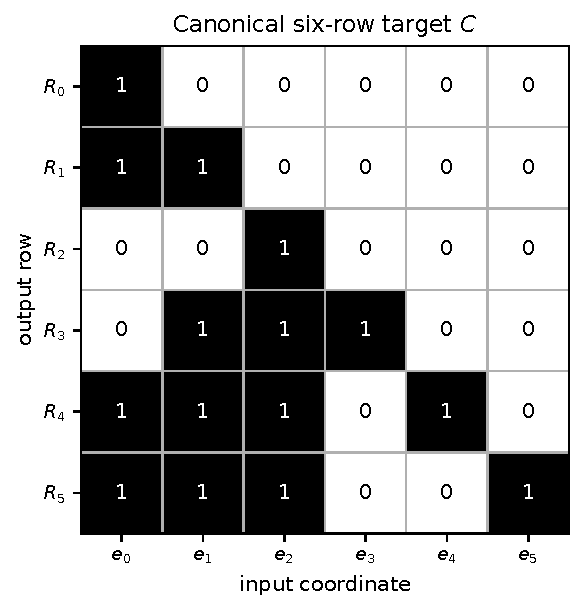
\includegraphics[width=.56\linewidth]{assets/g_canonical_matrix.pdf}
\caption{The canonical target $C$.  Black cells are nonzero.  Rows $0$ and $2$ are restored exactly, while rows $3,4,5$ require two distinct additions $v$ and $w$ from the source space $W$.}
\label{g:fig:canonical-matrix}
\end{figure}

\subsection{A six-gate ambient word}

\begin{proposition}\label{g:prop:ambient-upper}
For every nonzero commutative ring $R$ with identity,
\[
\ellAll(C)\le6.
\]
\end{proposition}

\begin{proof}
Apply the following six gates:
\begin{align}
R_1&\leftarrow R_1+R_2,\label{g:gate:a1}\\
R_3&\leftarrow R_3+R_1,\label{g:gate:a2}\\
R_1&\leftarrow R_1+R_0,\label{g:gate:a3}\\
R_4&\leftarrow R_4+R_1,\label{g:gate:a4}\\
R_5&\leftarrow R_5+R_1,\label{g:gate:a5}\\
R_1&\leftarrow R_1-R_2.\label{g:gate:a6}
\end{align}
After \cref{g:gate:a1}, row $1$ contains $v$.  Gate \cref{g:gate:a2} copies $v$ to row $3$.  Gate \cref{g:gate:a3} changes the carrier to $w$, which is copied to rows $4$ and $5$ by \cref{g:gate:a4,g:gate:a5}.  Gate \cref{g:gate:a6} removes the temporary $e_2$ component, leaving $e_1+e_0$.  Every row now agrees with $C$.
\end{proof}

\begin{figure}[t]
\centering
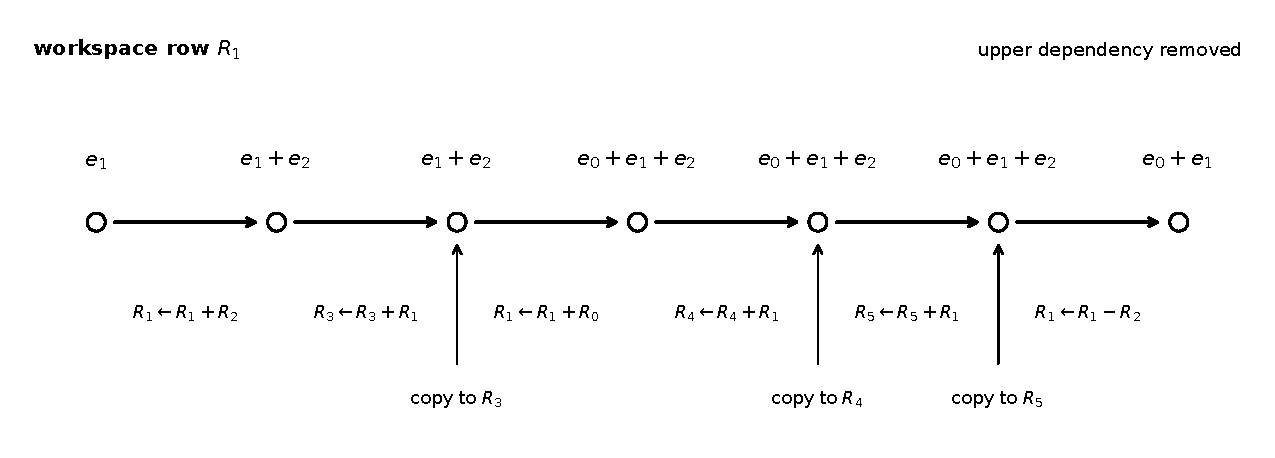
\includegraphics[width=.98\linewidth]{assets/g_carrier_timeline.pdf}
\caption{Carrier timeline for the six-gate ambient word.  The two upper-directed operations are the opening and closing gates on row $1$.  The state $e_1+e_2$ is exported once and $e_0+e_1+e_2$ is exported twice.}
\label{g:fig:carrier-timeline}
\end{figure}

\subsection{A seven-gate lower word}

\begin{proposition}\label{g:prop:lower-upper}
For every nonzero commutative ring $R$ with identity,
\[
\ellDown(C)\le7.
\]
\end{proposition}

\begin{proof}
The lower-directed word
\begin{align*}
R_1&\leftarrow R_1+R_0,\\
R_2&\leftarrow R_2+R_1,\\
R_3&\leftarrow R_3-R_0,\\
R_3&\leftarrow R_3+R_2,\\
R_4&\leftarrow R_4+R_2,\\
R_5&\leftarrow R_5+R_2,\\
R_2&\leftarrow R_2-R_1
\end{align*}
produces $C$.  After the first two gates, row $2$ contains $w$.  Rows $4$ and $5$ copy that state.  The two gates on row $3$ cancel the unwanted $e_0$ and leave $v$.  The final gate restores row $2$.
\end{proof}

\subsection{Restricted lower bound}

\begin{proposition}\label{g:prop:lower-lower-bound}
For every nonzero commutative ring $R$ with identity,
\[
\ellDown(C)\ge7.
\]
\end{proposition}

\begin{proof}
Rows $1,3,4,5$ differ from their initial values, so they must each be targeted.  Assume for contradiction that a lower-directed word of length at most six produces $C$.

First suppose row $2$ is never targeted.  Row $0$ remains $e_0$, row $2$ remains $e_2$, and every state ever assumed by row $1$ lies in $\Span(e_0,e_1)$ because the only possible source below row $1$ is row $0$.  Every output row retains coefficient $1$ on its own pivot coordinate in a lower-directed circuit, so no output row can lie in $W$.  Hence no available source row is a unit multiple of either
\[
v=e_1+e_2
\quad\text{or}\quad
w=e_0+e_1+e_2.
\]
By \cref{g:lem:one-target-source}, each of rows $3,4,5$ must be targeted at least twice.  Together with the required targeting of row $1$, this gives at least seven gates.

Now suppose row $2$ is targeted.  Since its final value is $e_2$, \cref{g:lem:target-count} forces at least two targetings of row $2$.  A six-gate word must therefore target row $2$ exactly twice and each of rows $1,3,4,5$ exactly once.  Each output row $3,4,5$ must receive its complete addition in its unique targeting.  Row $0$ cannot supply $v$ or $w$, and row $1$ never contains an $e_2$ component.  Therefore row $2$ must supply all three outputs, up to unit scaling.  But two targetings of row $2$ expose at most one noninitial intermediate state before row $2$ returns to $e_2$, while the outputs require both distinct states $v$ and $w$.  This is impossible.
\end{proof}

\subsection{Ambient lower bound}

\begin{proposition}\label{g:prop:ambient-lower-bound}
For every nonzero commutative ring $R$ with identity,
\[
\ellAll(C)\ge6.
\]
\end{proposition}

\begin{proof}
Assume that an ambient word of length at most five produces $C$.  Rows $1,3,4,5$ must each be targeted.  Rows $0$ and $2$ are unchanged.  If either were targeted, it would require at least two targetings, giving at least six gates in total.  Thus rows $0$ and $2$ are never targeted.  If all four changed rows are targeted once, each has only its initial and final state.  No such source is a unit multiple of $v=e_1+e_2$ or $w=e_0+e_1+e_2$, so the output rows cannot be completed.  In the only remaining case, exactly one of rows $1,3,4,5$ is targeted twice and the other three are targeted once.

Project the rows to the quotient module $R^6/W$.  Rows $0,1,2$ have zero image, while rows $3,4,5$ begin and end at the three distinct quotient basis vectors of the free quotient module.  An output row targeted exactly once must therefore use a source lying in $W$, by \cref{g:lem:one-target-source}.

Suppose first that row $1$ is the twice-targeted row.  The three output rows are each targeted once.  Rows $0$ and $2$ supply only scalar multiples of $e_0$ and $e_2$.  Row $1$ begins at $e_1$, has one intermediate state, and ends at $e_1+e_0$.  Thus at most one of the two required unit-multiple classes of $v$ and $w$ can appear as an available source.  The three outputs require both, a contradiction.

Suppose instead that an output row, say row $r\in\{3,4,5\}$, is targeted twice.  The other two outputs and row $1$ are targeted once.  We claim that row $r$ cannot lie in $W$ between its two targetings.  To cancel its unique quotient pivot $e_r$ at the first targeting, the source would already have to contain an $e_r$ component.  Before row $r$ is first targeted, the only way another row can acquire such a component is to be targeted using row $r$ as source.  That other row is targeted only once and would then retain an unwanted $e_r$ component in its final value.  Therefore row $r$ never becomes a $W$-valued carrier.  The only $W$-valued source states are rows $0$ and $2$ and the two states of singly targeted row $1$, namely its initial and final states.  None supplies both $v$ and $w$.  The two singly targeted outputs cannot be completed, again a contradiction.
\end{proof}

\begin{proof}[Proof of \cref{g:thm:universal-atom}]
Combine \cref{g:prop:ambient-upper,g:prop:lower-upper,g:prop:lower-lower-bound,g:prop:ambient-lower-bound}.
\end{proof}

\begin{remark}
The proof uses only unimodular rows, unit coordinates, and pivot support.  It does not use division or a characteristic assumption.  In characteristic two the closing subtraction equals addition.
\end{remark}

\begin{corollary}[Failure of geodesic convexity]\label{g:cor:nonconvex}
For every field $\F$ and every $n\ge6$, the lower-unitriangular frame subgraph is not geodesically convex in the transvection Cayley graph of $\Egrp_n(\F)=\SL_n(\F)$.
\end{corollary}

\begin{proof}
Embed $C$ as $C\oplus I_{n-6}$.  A six-gate ambient word acts on the first six rows.  In a lower-directed circuit, rows with index at least six cannot be used as sources for targets among the first six rows, so the restricted lower bound of seven persists.
\end{proof}

For the remainder of the paper, unless explicitly stated otherwise, the coefficient domain is a field $\F$.

\section{Catalytic normal forms and the six-role threshold}\label{g:sec:catalysis}

The universal atom is one instance of a root-conjugation mechanism.  This section isolates that mechanism and explains the count twenty.

\subsection{Root conjugation identities}

Let $p<q<y$ and $x<p<q$.  Direct multiplication gives
\begin{equation}\label{g:eq:read-conjugation}
\tau_{p,q}(-a)\,\tau_{y,p}(b)\,\tau_{p,q}(a)
=
\tau_{y,p}(b)\,\tau_{y,q}(ab),
\end{equation}
and
\begin{equation}\label{g:eq:update-conjugation}
\tau_{p,q}(-a)\,\tau_{q,x}(b)\,\tau_{p,q}(a)
=
\tau_{q,x}(b)\,\tau_{p,x}(-ab).
\end{equation}
A single forbidden upper transvection can therefore turn one lower interaction into two lower effects.  Interactions of the forms $x\to p$ and $q\to y$ commute through the excursion without duplication.  We call the duplicated interactions \emph{cross interactions} and the unduplicated interactions \emph{phase interactions}.

\begin{definition}[Simple one-catalyst word]\label{g:def:simple-catalyst}
A simple one-catalyst word has the form
\[
\tau_{p,q}(-a)\,h_m\cdots h_1\,\tau_{p,q}(a),
\qquad p<q,
\]
where every $h_i$ is lower directed and is one of
\[
\tau_{q,x}(b),\quad \tau_{p,x}(b),\quad
\tau_{y,p}(b),\quad \tau_{y,q}(b)
\]
with $x<p<q<y$.  Auxiliary rows are distinct unless stated otherwise.
\end{definition}

The circuit is read from right to left in the matrix product and from left to right as a gate list.  The opening and closing operations temporarily place the $q$ component in row $p$.

\begin{proposition}[Cross-interaction accounting]\label{g:prop:cross-accounting}
Let a simple one-catalyst word have $m$ middle interactions, of which $c$ are cross interactions.  Its target admits a lower-directed realization of length at most
\[
m+c.
\]
Consequently, if the ambient word of length $m+2$ is strictly shorter than every lower word, then
\[
c\ge3.
\]
\end{proposition}

\begin{proof}
Conjugate each middle generator using \cref{g:eq:read-conjugation,g:eq:update-conjugation}.  A phase interaction remains one lower transvection, while a cross interaction becomes a product of two lower transvections.  This gives length at most $m+c$.  If $c\le2$, then $m+c\le m+2$, so the ambient excursion cannot be strictly better.
\end{proof}

Three consumers are therefore the first possible point at which the cost two of opening and closing can be amortized.

\subsection{Why an all-cross word is insufficient}

Within the distinct-leaf normal form, cross count alone is not enough.

\begin{lemma}[All-cross mirror]\label{g:lem:all-cross-mirror}
Suppose a simple one-catalyst word contains only cross interactions, with left inputs $X$ and right outputs $Y$.  Then its target has a lower-directed realization with the same number of gates.
\end{lemma}

\begin{proof}
Write the opening coefficient as $a\in\F^\times$, the left-update coefficients as $b_x$, and the right-read coefficients as $c_y$.  Since the all-cross middle gates commute past one another, the ambient gate list may be written
\[
R_p\leftarrow R_p+aR_q;
\quad
[R_q\leftarrow R_q+b_xR_x]_{x\in X};
\quad
[R_y\leftarrow R_y+c_yR_p]_{y\in Y};
\quad
R_p\leftarrow R_p-aR_q.
\]
Put $B=\sum_{x\in X}b_xe_x$.  Its final nontrivial rows are
\[
R_p=e_p-aB,
\qquad
R_q=e_q+B,
\qquad
R_y=e_y+c_ye_p+ac_ye_q
\quad(y\in Y).
\]
The following lower-directed gate list produces the same rows:
\[
R_q\leftarrow R_q+a^{-1}R_p;
\quad
[R_y\leftarrow R_y+ac_yR_q]_{y\in Y};
\quad
[R_p\leftarrow R_p-ab_xR_x]_{x\in X};
\quad
R_q\leftarrow R_q-a^{-1}R_p.
\]
Indeed, after the first gate $R_q=e_q+a^{-1}e_p$, so the output gates create exactly $c_ye_p+ac_ye_q$.  The source updates then leave $R_p=e_p-aB$, and the final gate changes $R_q$ to $e_q+B$.  Both words have $|X|+|Y|+2$ gates.
\end{proof}

Thus a minimal strict shortcut needs both positive catalytic excess and a phase switch that makes temporal order matter.

\begin{proposition}[Six-role threshold in the simple model]\label{g:prop:six-role}
A strict shortcut in the distinct-leaf simple one-catalyst model requires at least six row roles:
\[
2\text{ catalyst rows}
+
3\text{ cross interactions}
+
1\text{ phase interaction}.
\]
The bound is attained by the matrix $C$.
\end{proposition}

\begin{proof}
By \cref{g:prop:cross-accounting}, at least three cross interactions are required.  By \cref{g:lem:all-cross-mirror}, at least one phase interaction is required.  With distinct leaves these use four auxiliary rows in addition to the two catalyst rows.  The word of \cref{g:prop:ambient-upper} has exactly this form.
\end{proof}

\begin{figure}[t]
\centering
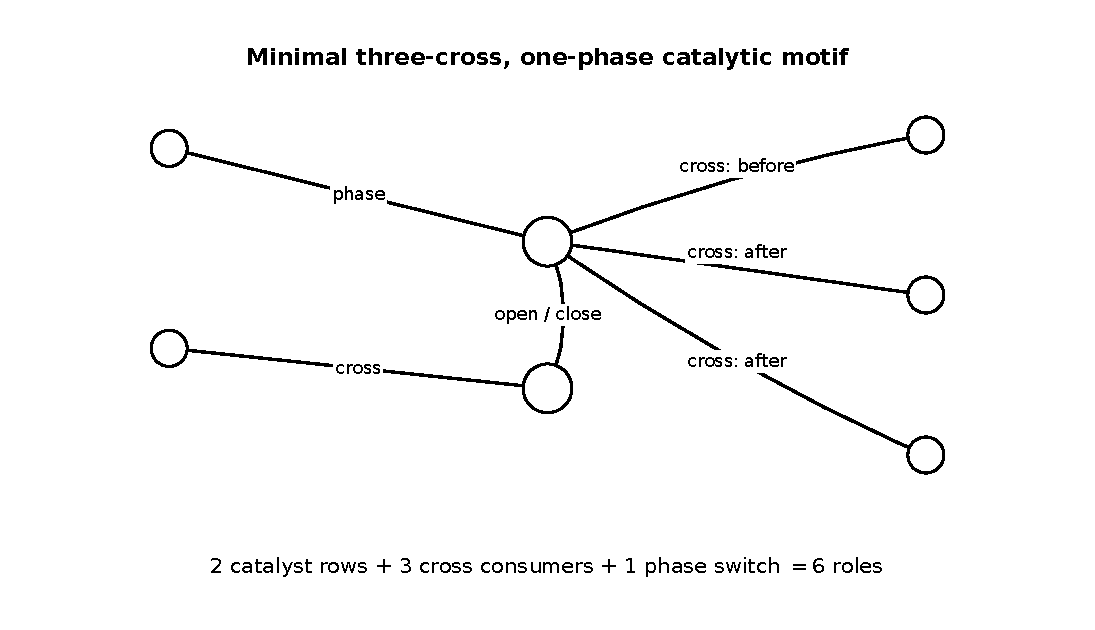
\includegraphics[width=.82\linewidth]{assets/g_catalytic_motif.pdf}
\caption{The minimal one-catalyst motif.  Cross interactions reuse the opened carrier.  The phase gate separates consumers that observe two different carrier states and prevents the all-cross mirror.}
\label{g:fig:catalytic-motif}
\end{figure}

\subsection{Enumeration of the minimal motifs}

Fix six ordered rows.  The catalyst pair must be adjacent in a minimal six-role word.  Write
\[
p<q=p+1,
\]
let $L$ be the set of rows left of $p$, and let $R$ be the set of rows right of $q$.  Then
\[
|L|+|R|=4,
\qquad
|L|,|R|>0.
\]
There are two orientations.

\paragraph{Left phase.}
Choose a phase leaf $x\in L$.  The remaining $|L|-1$ left leaves interact by $u\to q$.  Every right leaf is a cross read $p\to y$.  To make the phase effective, the right leaves are divided into a nonempty set read before $x\to p$ and a nonempty set read after it.  The number of targets is
\[
|L|\bigl(2^{|R|}-2\bigr).
\]

\paragraph{Right phase.}
Choose a phase leaf $y\in R$.  Every other right leaf is a cross read.  The left updates into $q$ are divided nontrivially before and after the phase gate $q\to y$.  The number is
\[
|R|\bigl(2^{|L|}-2\bigr).
\]

\begin{proposition}[Motif count]\label{g:prop:motif-count}
For a split $(L,R)=(|L|,|R|)$ with $L+R=4$, the number of minimal phase-separated targets is
\[
N_{L,R}
=L(2^R-2)+R(2^L-2).
\]
For the three possible splits,
\[
N_{1,3}=6,
\qquad
N_{2,2}=8,
\qquad
N_{3,1}=6.
\]
Hence there are twenty targets.
\end{proposition}

\begin{proof}
The preceding left-phase and right-phase constructions are disjoint because the phase row lies on opposite sides of the catalyst.  Within each orientation, the final support records the phase leaf and the before/after subset, so distinct choices give distinct targets.  Summing gives the formula and the stated values.
\end{proof}

\begin{figure}[t]
\centering
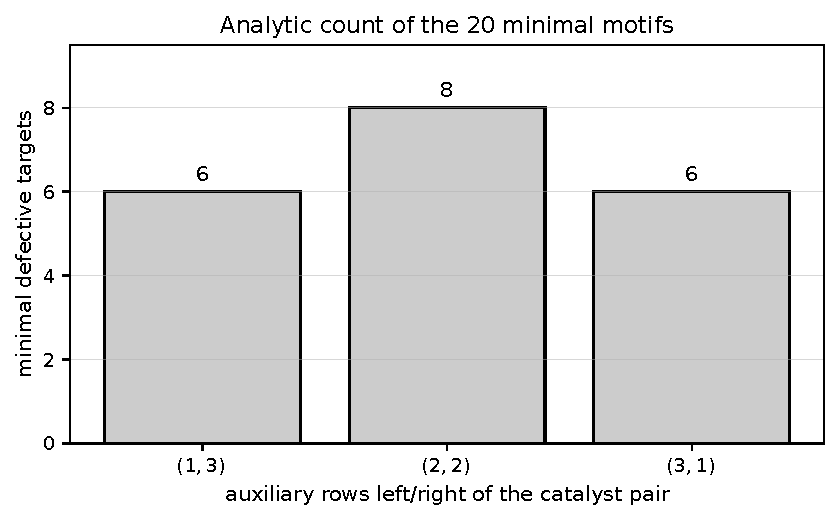
\includegraphics[width=.70\linewidth]{assets/g_motif_count.pdf}
\caption{The analytic count of the twenty minimal catalytic targets.}
\label{g:fig:motif-count}
\end{figure}

Every target counted by \cref{g:prop:motif-count} has an explicit six-gate ambient word and a seven-gate lower word obtained by eliminating the three cross interactions.  The nontrivial statement is that there are no other defects in dimension six and that none of these targets has a lower word of length six.  That is the exact classification established in \cref{g:sec:enumeration}.

\section{Exact finite enumeration}\label{g:sec:enumeration}

This section describes the computer-assisted part of the paper.  The computations use integer encodings only.  No floating-point decisions occur.

\subsection{Restricted breadth-first search}

Over $\F_2$, an element of $\U_n(\F_2)$ is determined by its $n(n-1)/2$ strict lower entries.  For $n=6$ there are $2^{15}=32768$ states.  Breadth-first search from the identity using the fifteen lower transvections gives every restricted distance and the restricted diameter.

For $n=6$, the restricted diameter is eight.  Therefore every lower-unitriangular target has ambient distance at most eight.  This makes a radius-four meet-in-the-middle search complete.

\subsection{Ambient radius-four ball and right-coset pairing}

Let
\[
B_4=\{g\in\GL_6(\F_2):\ellAll(g)\le4\}.
\]
Exact breadth-first search gives
\[
|B_4|=110626.
\]
Group $B_4$ by right cosets of $\U_6(\F_2)$.  If $a,b$ lie in the same right coset, then
\[
b^{-1}a\in\U_6(\F_2),
\]
and
\[
\ellAll(b^{-1}a)\le\ellAll(b)+\ellAll(a)\le8.
\]
The implementation uses a canonical right-coset key obtained by reducing matrix columns from right to left.  Right multiplication by a lower-unitriangular matrix changes column $j$ only by a combination of columns with larger index, so this reduction is constant on right cosets and separates them.

\begin{lemma}[Meet-in-the-middle completeness]\label{g:lem:mitm-complete}
For every $u\in\U_6(\F_2)$,
\[
\ellAll(u)
=
\min\{\ellAll(a)+\ellAll(b):a,b\in B_4,\ b^{-1}a=u\}.
\]
\end{lemma}

\begin{proof}
Every pair on the right gives a word for $u$, so the right-hand side is at least $\ellAll(u)$.  Conversely, $\ellAll(u)\le8$.  Take a shortest path from the identity to $u$ and split it at a midpoint.  The prefix endpoint $a$ has distance at most four.  The inverse of the remaining suffix is an element $b$ of distance at most four, and $u=b^{-1}a$.  Hence the minimum is at most $\ellAll(u)$.
\end{proof}

The radius-four ball splits into $6948$ right-coset buckets.  The largest bucket has $3775$ elements.  The computation checks $45178326$ ordered pairs and recovers an ambient distance for every one of the $32768$ targets.

\subsection{The exact binary census}

\begin{table}[t]
\centering
\caption{Complete distance distribution in $\U_6(\F_2)$.}
\label{g:tab:census}
\begin{tabular}{@{}rrr@{}}
\toprule
$\ellDown$ & $\ellAll$ & number of targets\\
\midrule
0&0&1\\
1&1&15\\
2&2&125\\
3&3&720\\
4&4&2914\\
5&5&7851\\
6&6&12656\\
7&6&20\\
7&7&7926\\
8&8&540\\
\bottomrule
\end{tabular}
\end{table}

\begin{figure}[t]
\centering
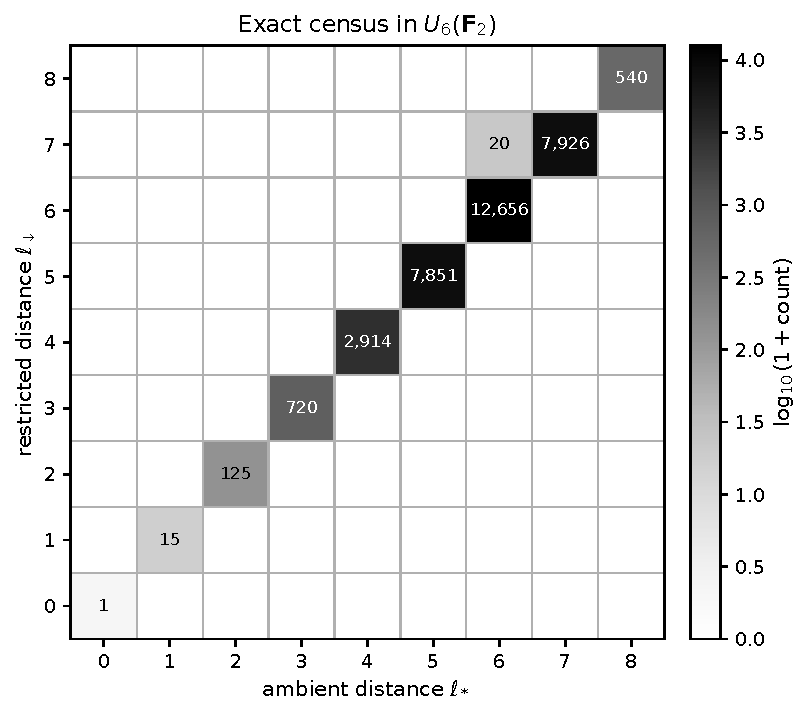
\includegraphics[width=.72\linewidth]{assets/g_distance_census.pdf}
\caption{Complete binary dimension-six census.  The only off-diagonal cell contains the twenty targets with distance pair $(7,6)$.}
\label{g:fig:distance-census}
\end{figure}

\begin{proof}[Proof of \cref{g:thm:binary-census}]
For $n=2,3,4,5$, complete restricted breadth-first search and complete ambient meet-in-the-middle search return zero defects.  The state counts are respectively $2,8,64,1024$.  For $n=6$, \cref{g:lem:mitm-complete} proves that the ambient calculation is exhaustive.  The resulting distribution is \cref{g:tab:census}; its counts sum to $32768$, no target is missing, and the only strict pair is $(7,6)$ with multiplicity twenty.
\end{proof}

\begin{proof}[Proof of \cref{g:thm:motif-classification}]
The analytic generator of \cref{g:prop:motif-count} produces twenty distinct targets without reference to the distance census.  Exact set comparison shows that these twenty targets are precisely the twenty off-diagonal targets in \cref{g:tab:census}.  Each therefore has distances $(7,6)$, and no other dimension-six target is defective.
\end{proof}

\subsection{Ternary and additional field checks}

For $\F_3$, every nonzero scaled transvection is included.  Complete searches give the data in \cref{g:tab:small-fields}.

\begin{table}[t]
\centering
\caption{Complete no-defect computations below dimension six.}
\label{g:tab:small-fields}
\begin{tabular}{@{}crrr@{}}
\toprule
field & $n$ & $|\U_n(\F)|$ & restricted diameter\\
\midrule
$\F_2$&2&2&1\\
$\F_2$&3&8&2\\
$\F_2$&4&64&4\\
$\F_2$&5&1024&6\\
\addlinespace
$\F_3$&2&3&1\\
$\F_3$&3&27&3\\
$\F_3$&4&729&5\\
$\F_3$&5&59049&7\\
\bottomrule
\end{tabular}
\end{table}

The $n=5$ ternary computation uses radius-three and radius-four balls, checks $38415205$ right-coset pairs, and recovers all $59049$ targets.  It finds no defect.  The field-independent \cref{g:thm:universal-atom} supplies a defect at $n=6$, proving \cref{g:thm:ternary-threshold}.  Separate exact searches over $\F_3$ and $\F_5$ verify the distances of the canonical atom directly.  The $\F_5$ calculation is an audit of the atom, not a complete threshold computation below dimension six.

\subsection{Verification status}

The analytic proofs of \cref{g:thm:universal-atom,g:cor:linear-gap} do not depend on computation.  The claims in \cref{g:thm:binary-census,g:thm:motif-classification,g:thm:ternary-threshold} depend on exact finite enumeration.  The source archive contains:
\begin{itemize}
\item the C++ programs for every breadth-first and meet-in-the-middle search;
\item the Python program that independently generates the twenty motifs and compares sets;
\item symbolic checks for the bounded-resource formulas and the totally unimodular $M(K_4)$ representation;
\item exact stdout files and JSON packet data;
\item SHA-256 checksums;
\item build and reproduction commands.
\end{itemize}
The programs were rebuilt from source and rerun independently when this manuscript was assembled; the outputs matched byte for byte.

\section{Projective, matroidal, and spectral structure}\label{g:sec:geometry-spectrum}

\subsection{The flagged Pasch packet}

Over $\F_2$, write
\[
x=e_0,
\qquad
p=e_1,
\qquad
q=e_2.
\]
The canonical ambient word uses the six nonzero vectors
\[
x,
\quad p,
\quad q,
\quad p+q,
\quad p+q+x,
\quad p+x
\]
inside $\Span(x,p,q)\cong\F_2^3$.  The only missing nonzero vector is $x+q$.

In $\operatorname{PG}(2,2)$, three distinct points form a line exactly when their vector representatives sum to zero.  The six points support the four lines
\[
\{x,p,x+p\},
\quad
\{x,p+q,x+p+q\},
\quad
\{p,q,p+q\},
\quad
\{x+p,q,x+p+q\}.
\]
Every point lies on exactly two of these lines.  This is the Pasch configuration, equivalently the Fano plane with one point and its three incident lines removed from the full incidence structure.

\begin{figure}[t]
\centering
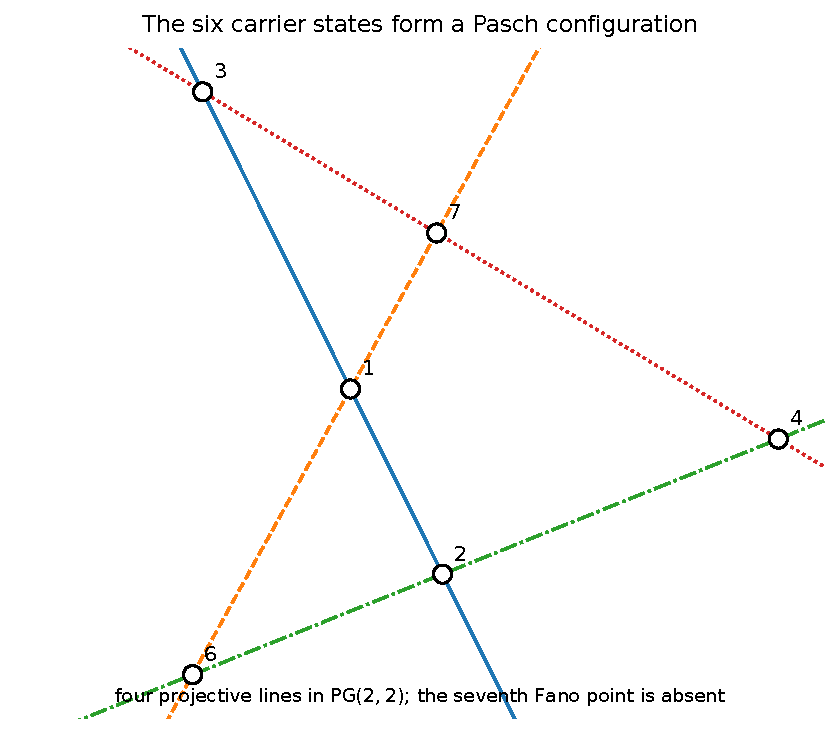
\includegraphics[width=.65\linewidth]{assets/g_pasch_configuration.pdf}
\caption{A real drawing of the four-line Pasch incidence structure.  The labels are the binary point encodings $1,2,3,4,6,7$; point $5$ is the missing Fano point.}
\label{g:fig:pasch}
\end{figure}

The configuration is flagged because the rows have fixed roles.  Points $x$ and $q$ are stationary sources, $p$ is the carrier, and the remaining points occur as carrier states.  Forgetting those roles loses the circuit ordering information.

\subsection{The regular matroid \texorpdfstring{$M(K_4)$}{M(K4)}}

The six carrier states admit a field-independent representation.  In the ordered basis $(x,p,q)$, place them as the columns of
\begin{equation}\label{g:eq:k4-matrix}
B=
\begin{pmatrix}
1&0&0&1&0&1\\
0&1&0&1&1&1\\
0&0&1&0&1&1
\end{pmatrix},
\end{equation}
corresponding respectively to
\[
x,
\quad p,
\quad q,
\quad x+p,
\quad p+q,
\quad x+p+q.
\]

\begin{proposition}[Regular-matroid core]\label{g:prop:regular-matroid}
Every square minor of $B$ belongs to $\{0,\pm1\}$, so $B$ is totally unimodular.  Hence the column-dependence matroid is the same over every field.  Under the edge labeling
\[
\begin{array}{c|cccccc}
\text{state}&p&x&x+p&p+q&q&x+p+q\\
\hline
K_4\text{ edge}&12&13&23&14&24&34,
\end{array}
\]
it is the graphic matroid $M(K_4)$.
\end{proposition}

\begin{proof}
A direct calculation of all square minors of $B$ gives only $0$, $1$, and $-1$.  Thus every subdeterminant has characteristic-independent vanishing, and a column set is independent over one field exactly when it is independent over every field.  The four minimal dependent triples are
\[
\{x,p,x+p\},
\quad
\{p,q,p+q\},
\quad
\{x,p+q,x+p+q\},
\quad
\{q,x+p,x+p+q\}.
\]
Under the displayed edge labeling, these are precisely the four triangular cycles of $K_4$.  They determine the rank-three cycle matroid $M(K_4)$, which is regular because it has a totally unimodular representation; see, for example, \cite{g:Oxley2011}.
\end{proof}

\begin{figure}[t]
\centering
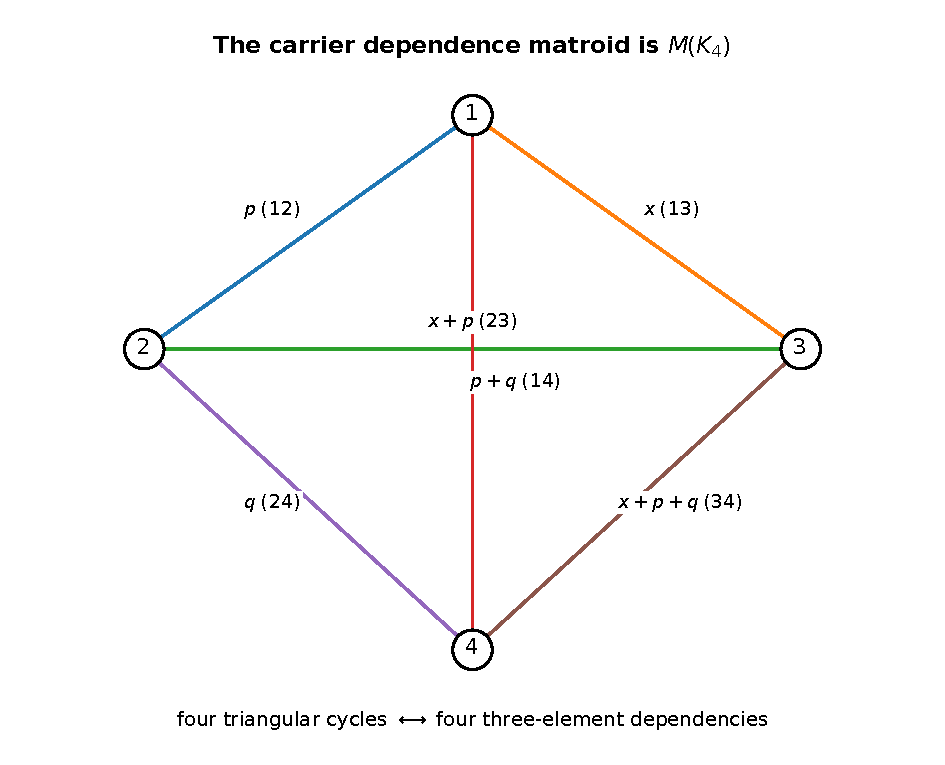
\includegraphics[width=.72\linewidth]{assets/g_regular_matroid_k4.pdf}
\caption{The six carrier states as the edges of $K_4$.  Each triangular cycle is one of the four three-element dependencies in the Pasch configuration.  The resulting regular matroid is representable over every field.}
\label{g:fig:k4-matroid}
\end{figure}

The field-independent circuit theorem is stronger than matroid representability alone, because it also depends on the ordering and the designated carrier role.  Nevertheless, \cref{g:prop:regular-matroid} explains why the local dependence pattern survives unchanged in every characteristic.

\subsection{Distance as first arrival}

Let $G$ be a finite group and $S=S^{-1}$ a symmetric generating set.  On $\ell^2(G)$, let $\lambda$ be the left regular representation,
\[
\lambda(s)\delta_h=\delta_{sh},
\]
and define
\[
A_S=\sum_{s\in S}\lambda(s).
\]
For $g\in G$, define the endpoint Green series
\[
\mathcal G_{S,g}(z)
=
\left\langle
\delta_g,
(I-zA_S)^{-1}\delta_e
\right\rangle.
\]

\begin{proposition}[First-arrival identity]\label{g:prop:first-arrival}
The coefficient of $z^k$ in $\mathcal G_{S,g}(z)$ is the number of length-$k$ words in $S$ with product $g$.  Hence
\[
d_S(e,g)=\ord_{z=0}\mathcal G_{S,g}(z).
\]
\end{proposition}

\begin{proof}
Formally,
\[
(I-zA_S)^{-1}=\sum_{k\ge0}z^kA_S^k.
\]
The matrix coefficient $\langle\delta_g,A_S^k\delta_e\rangle$ counts $k$-step walks from $e$ to $g$, which are exactly length-$k$ words with product $g$.  The first nonzero coefficient occurs at the word distance.
\end{proof}

If
\[
A_S=\sum_\lambda \lambda\Pi_\lambda
\]
is the spectral resolution, then
\[
\mathcal G_{S,g}(z)
=
\sum_\lambda
\frac{\langle\delta_g,\Pi_\lambda\delta_e\rangle}{1-\lambda z}.
\]
Thus eigenvalues alone do not determine first arrival.  The endpoint matrix coefficients of the spectral projectors are essential.

For the canonical target $C$, exact word counts begin
\begin{align*}
\mathcal G_{\downarrow,C}(z)
&=
543z^7+25080z^8+510703z^9+10824940z^{10}+\cdots,\\
\mathcal G_{*,C}(z)
&=
2z^6+776z^7+39454z^8+\cdots.
\end{align*}
The metric defect is the valuation drop
\[
\ord_0\mathcal G_{\downarrow,C}
-
\ord_0\mathcal G_{*,C}
=1.
\]

\begin{figure}[t]
\centering
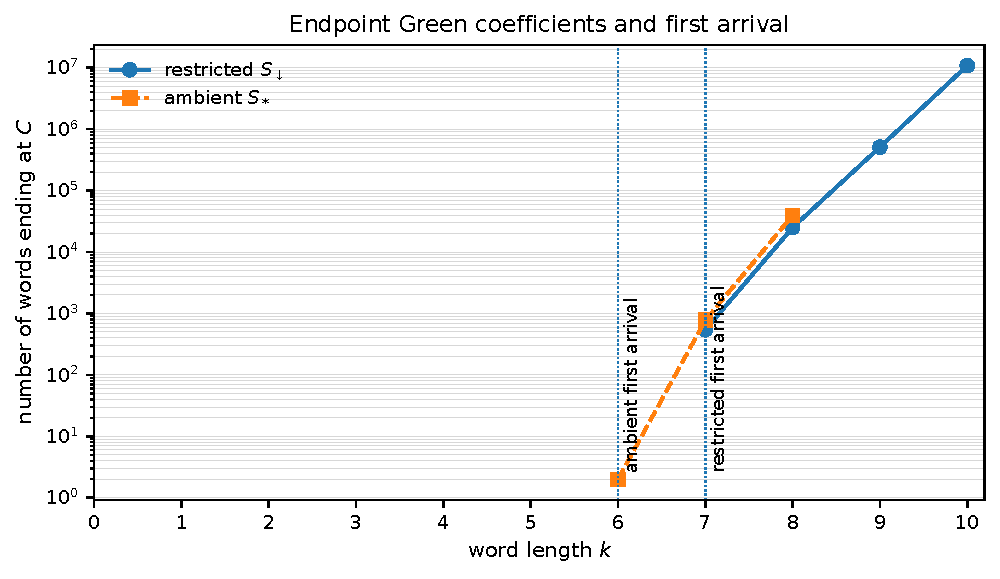
\includegraphics[width=.78\linewidth]{assets/g_green_coefficients.pdf}
\caption{Exact endpoint word counts for the canonical target.  The ambient walk first arrives at length six.  The restricted walk first arrives at length seven.}
\label{g:fig:green-coefficients}
\end{figure}

Across the twenty defects, the truncated endpoint data split into five Green-signature classes, each of multiplicity four.  The signatures are listed in \cref{g:tab:green-signatures}.

\begin{table}[t]
\centering
\caption{The five endpoint Green-signature packets.  Each row occurs for four defective targets.}
\label{g:tab:green-signatures}
\resizebox{\textwidth}{!}{%
\begin{tabular}{@{}rrrrrrrr@{}}
\toprule
&\multicolumn{4}{c}{restricted coefficients}&\multicolumn{3}{c}{ambient coefficients}\\
packet&$[z^7]$&$[z^8]$&$[z^9]$&$[z^{10}]$&$[z^6]$&$[z^7]$&$[z^8]$\\
\midrule
1&326&15430&316118&7576819&4&570&23318\\
2&326&15536&321870&7727183&4&570&23318\\
3&543&25080&510703&10824940&2&776&39454\\
4&543&25639&511524&10984988&2&776&39454\\
5&543&26091&511819&11121486&2&776&39454\\
\bottomrule
\end{tabular}}
\end{table}

\section{Interval-tree certificates and connected higher-dimensional families}\label{g:sec:higher}

From this point through the rank and tensor arguments, the coefficient domain is a field $\F$.  The six-row atom is the first defect, but it is not an isolated low-dimensional accident.  This section gives a field-independent family of connected targets in every dimension at least seven.  The lower bound is certified by a multiscale rank potential adapted to the ordered flag.

\subsection{Interval-tree rank potential}

\begin{definition}[Interval tree]
An \emph{interval tree} on the ordered coordinates $0,1,\ldots,n-1$ is a rooted binary tree whose leaves occur in that order and whose every node is a contiguous interval.  If an internal node $v$ splits its interval into consecutive left and right children $L_v$ and $R_v$, define
\begin{equation}\label{g:eq:tree-potential}
\Phi_T(A)
=
\sum_{v\in\operatorname{Int}(T)}
\rank A[R_v,L_v],
\qquad A\in\U_n(\F).
\end{equation}
\end{definition}

\begin{lemma}[One-cut locality]\label{g:lem:one-cut-locality}
Let $X\in\U_n(\F)$ and let $X'$ be obtained from $X$ by one lower-directed transvection.  Then
\[
\bigl|\Phi_T(X')-\Phi_T(X)\bigr|\le1.
\]
\end{lemma}

\begin{proof}
Suppose the gate is $s\to t$ with $s<t$.  Let $v_0$ be the lowest node of $T$ whose two children separate $s$ and $t$.  The order of the leaves forces $s\in L_{v_0}$ and $t\in R_{v_0}$.  At this one node, a single row of the cross block $X[R_{v_0},L_{v_0}]$ changes, so its rank changes by at most one.

At every ancestor of $v_0$, the two rows lie in the same child.  If that child is the right child, the gate is an internal row operation on the relevant cross block and preserves rank; if it is the left child, the cross block is unchanged.  At a descendant containing $t$ but not $s$, every column of the descendant interval lies strictly to the right of $s$.  Since $X$ remains lower triangular, row $s$ vanishes on those columns, so the descendant block is unchanged.  All other descendants are also unchanged.  Hence only the term at $v_0$ can vary.
\end{proof}

\begin{corollary}[Interval-tree lower bound]\label{g:cor:tree-lower-bound}
For every $A\in\U_n(\F)$ and every interval tree $T$,
\[
\ellDown(A)\ge\Phi_T(A).
\]
\end{corollary}

\begin{proof}
The identity has potential zero.  Apply \cref{g:lem:one-cut-locality} along any lower-directed word from the identity to $A$.
\end{proof}

\begin{definition}[Tree-tight target]\label{g:def:tree-tight}
A lower-unitriangular target $A$ is \emph{tree tight} if some interval tree $T$ satisfies
\[
\Phi_T(A)=\ellDown(A).
\]
\end{definition}

Tree tightness is stronger than possessing a rank lower bound.  It says that one ordered hierarchy accounts for the entire restricted word length.  The family below is tree tight by construction.

\subsection{The snapshot family}

Fix integers
\[
u\ge1,
\qquad
1\le v\le u+1,
\]
and choose distinct phases
\[
0\le s_1<s_2<\cdots<s_v\le u.
\]
Order the coordinates as
\[
x_1,\ldots,x_u,\ p,\ q,\ t_1,\ldots,t_v.
\]
For $0\le s\le u$, put
\begin{equation}\label{g:eq:prefix-state}
w_s=e_p+\sum_{i=1}^{s}e_{x_i}.
\end{equation}
Define
\begin{equation}\label{g:eq:snapshot-target}
A(u;s_1,\ldots,s_v)\in\U_{u+v+2}(\F)
\end{equation}
by
\[
R_{x_i}=e_{x_i},
\qquad
R_p=w_u,
\qquad
R_q=e_q,
\]
and
\begin{equation}\label{g:eq:snapshot-output}
R_{t_j}=e_{t_j}+e_q+w_{s_j}
\qquad(1\le j\le v).
\end{equation}
The output rows record selected intermediate versions of the carrier $p$.

\begin{proof}[Proof of \cref{g:thm:snapshot-family}]
For the ambient construction, first apply
\[
q\to p.
\]
Sweep through the updates
\[
x_1\to p,\ldots,x_u\to p.
\]
Whenever phase $s_j$ is reached, apply
\[
p\to t_j.
\]
Finally apply $q\to p$ with coefficient $-1$.  At phase $s$, the carrier is $e_q+w_s$, so every output has the required value, and the final gate removes $e_q$ from row $p$.  The word has length
\[
1+u+v+1=u+v+2.
\]
Thus
\[
\ellAll\bigl(A(u;s_1,\ldots,s_v)\bigr)\le u+v+2.
\]

For a lower word, perform the same $u$ updates without opening the catalyst.  At each selected phase, use the two gates
\[
p\to t_j,
\qquad
q\to t_j.
\]
This gives length $u+2v$.

It remains to prove optimality in the lower model.  At the root, split
\[
\{x_1,\ldots,x_u,p\}
\quad\big|\quad
\{q,t_1,\ldots,t_v\}.
\]
The nonzero rows of the root cross block are $w_{s_1},\ldots,w_{s_v}$.  Distinct prefix vectors are linearly independent: in a linear relation, inspect successively a coordinate occurring in $w_{s_j}$ but in none of the earlier prefixes, starting from the largest phase.  Hence the root contributes $v$.

Inside the left child, use the comb that splits off $x_1$, then $x_2$, and so on while retaining $p$ in the remaining interval.  Every one of the $u$ cuts has rank one because the final row $p$ contains every $x_i$.  Inside the right child, repeatedly split off the last output while retaining $q$ in the left interval.  Each of the $v$ cuts has rank one because every output contains $q$.  Therefore
\[
\Phi_T\bigl(A(u;s_1,\ldots,s_v)\bigr)
=v+u+v=u+2v.
\]
The interval-tree lower bound matches the displayed lower circuit.
\end{proof}

\begin{figure}[t]
\centering
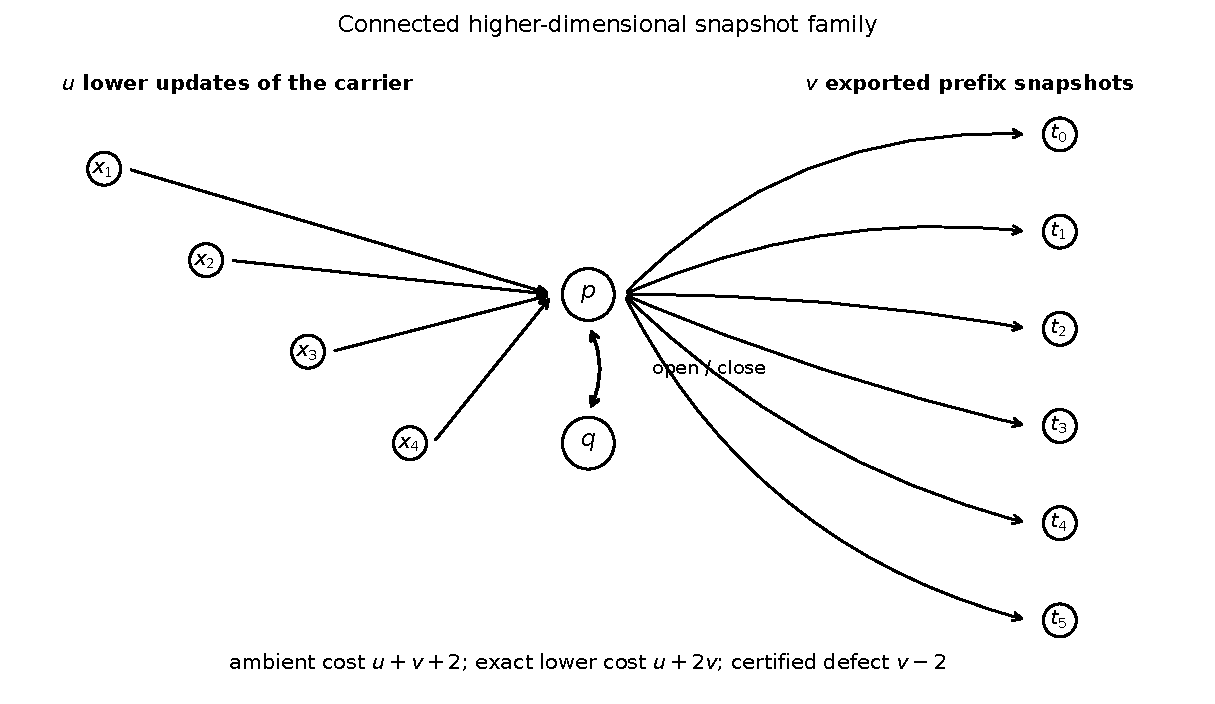
\includegraphics[width=.90\linewidth]{assets/g_snapshot_family.pdf}
\caption{The connected snapshot family.  One temporary upper dependency lets the ambient circuit export $v$ selected prefix states.  A lower-only circuit must insert the $q$ component separately into every output.}
\label{g:fig:snapshot-family}
\end{figure}

\begin{remark}[Support connectivity]
For $u,v\ge1$, the undirected support graph of $A(u;s_1,\ldots,s_v)-I$ is connected.  Row $p$ joins all update coordinates $x_i$, while every output joins both $p$ and $q$.  The separation below therefore does not arise from a direct sum of independent six-row gadgets.
\end{remark}

\subsection{Exact higher binary examples}

The interval tree gives the exact restricted distance in all dimensions.  For the first three higher targets, a separate bidirectional search also proves that the displayed ambient construction is optimal.

\begin{theorem}[Exact binary cases in dimensions seven through nine]\label{g:thm:higher-exact}
Over $\F_2$, let
\[
H_7=A(2;0,1,2),
\qquad
H_8=A(3;0,1,2),
\qquad
H_9=A(3;0,1,2,3).
\]
Then
\[
(\ellDown(H_7),\ellAll(H_7))=(8,7),
\]
\[
(\ellDown(H_8),\ellAll(H_8))=(9,8),
\]
and
\[
(\ellDown(H_9),\ellAll(H_9))=(11,9).
\]
\end{theorem}

\begin{proof}
The restricted values follow from \cref{g:thm:snapshot-family}.  The ambient words have lengths $7$, $8$, and $9$.  To exclude shorter words, the supplement computes exact ambient balls and checks that the two relevant balls do not intersect.  The certificate sizes are
\begin{center}
\begin{tabular}{@{}ccll@{}}
\toprule
$n$&tested split&left ball&right ball\\
\midrule
$7$&$3+3$&$23276$&$23276$\\
$8$&$3+4$&$52277$&$1174097$\\
$9$&$4+4$&$2994949$&$2994949$\\
\bottomrule
\end{tabular}
\end{center}
Every intersection is empty.  Since the generating sets are symmetric, an empty radius-$r$ versus radius-$s$ intersection rules out every word of length at most $r+s$.
\end{proof}

These are exact higher-dimensional examples, not merely padded copies of $C$.

\subsection{A connected defect in every dimension}

\begin{proof}[Proof of \cref{g:cor:connected-gap}]
For $n\ge7$, put
\[
v_n=\left\lfloor\frac{n-1}{2}\right\rfloor,
\qquad
u_n=n-v_n-2,
\]
and take the phases
\[
0,1,\ldots,v_n-1.
\]
The inequality $v_n\le u_n+1$ holds, so the snapshot target is defined.  By \cref{g:thm:snapshot-family},
\[
\ellDown(A_n)=u_n+2v_n=n+v_n-2,
\]
while
\[
\ellAll(A_n)\le u_n+v_n+2=n.
\]
Hence
\[
\ellDown(A_n)-\ellAll(A_n)
\ge v_n-2
=
\left\lfloor\frac{n-5}{2}\right\rfloor.
\]
Connectivity follows from the preceding remark.
\end{proof}

\begin{table}[t]
\centering
\caption{Successive connected cases from the optimized snapshot family.  The restricted value is exact; the ambient column is a certified construction and is exact for $n=7,8,9$ over $\F_2$.}
\label{g:tab:higher-cases}
\begin{tabular}{@{}rrrrr@{}}
\toprule
$n$&$u$&$v$&$\ellDown$&ambient upper bound / certified gap\\
\midrule
$7$&$2$&$3$&$8$&$7\;/\;1$\\
$8$&$3$&$3$&$9$&$8\;/\;1$\\
$9$&$3$&$4$&$11$&$9\;/\;2$\\
$10$&$4$&$4$&$12$&$10\;/\;2$\\
$11$&$4$&$5$&$14$&$11\;/\;3$\\
$12$&$5$&$5$&$15$&$12\;/\;3$\\
$13$&$5$&$6$&$17$&$13\;/\;4$\\
$15$&$6$&$7$&$20$&$15\;/\;5$\\
$17$&$7$&$8$&$23$&$17\;/\;6$\\
$19$&$8$&$9$&$26$&$19\;/\;7$\\
$21$&$9$&$10$&$29$&$21\;/\;8$\\
\bottomrule
\end{tabular}
\end{table}

\begin{figure}[t]
\centering
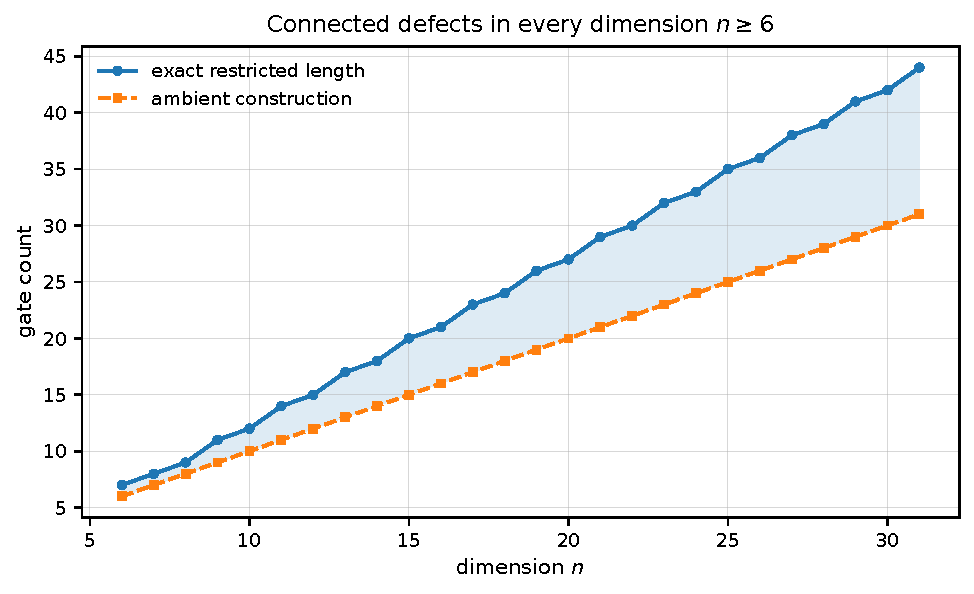
\includegraphics[width=.76\linewidth]{assets/g_connected_higher_cases.pdf}
\caption{The six-row atom is the first exact defect.  From dimension seven onward, the connected snapshot family gives an exact restricted length and a shorter ambient construction in every dimension.}
\label{g:fig:higher-cases}
\end{figure}

The ratio also increases beyond the block-sum value $7/6$.

\begin{corollary}[Asymptotic multiplicative distortion]\label{g:cor:three-halves}
For every field,
\[
\limsup_{n\to\infty}
\sup_{A\in\U_n(\F),\,A\ne I}
\frac{\ellDown(A)}{\ellAll(A)}
\ge\frac32.
\]
\end{corollary}

\begin{proof}
Along the optimized connected family,
\[
\frac{\ellDown(A_n)}{\ellAll(A_n)}
\ge
\frac{n+\lfloor(n-1)/2\rfloor-2}{n},
\]
which tends to $3/2$.
\end{proof}

\section{Bounded and weighted catalytic resources}\label{g:sec:resources}

The connected snapshot family uses a single matched excursion: one upper-directed gate opens the dirty carrier and one upper-directed gate closes it.  This permits a sharper statement than the unrestricted inequality $\ellAll<\ellDown$.

\subsection{A bounded number of upper-directed gates}

For a circuit word $w$, let $u(w)$ denote its number of upper-directed gates.

\begin{definition}[Upper-gate budget]
For $q\ge0$ and $A\in\U_n(\F)$, define
\[
\ellBudget{q}(A)
=
\min\{|w|:[w]=A,\ u(w)\le q\}.
\]
Thus
\[
\ellBudget{0}(A)=\ellDown(A),
\qquad
\ellBudget{q+1}(A)\le\ellBudget{q}(A),
\qquad
\ellAll(A)\le\ellBudget{q}(A).
\]
\end{definition}

\begin{proposition}[Two upper gates give a linear advantage]\label{g:prop:two-upper-linear}
For every snapshot target $A=A(u;s_1,\ldots,s_v)$,
\[
\ellBudget{0}(A)=u+2v,
\qquad
\ellBudget{2}(A)\le u+v+2.
\]
Consequently,
\[
\ellBudget{0}(A)-\ellBudget{2}(A)\ge v-2.
\]
For the optimized connected target $A_n$ of \cref{g:cor:connected-gap},
\[
\ellBudget{0}(A_n)-\ellBudget{2}(A_n)
\ge
\left\lfloor\frac{n-5}{2}\right\rfloor.
\]
\end{proposition}

\begin{proof}
The exact restricted value is \cref{g:thm:snapshot-family}.  Its ambient construction has precisely two upper-directed gates, namely the opening and closing operations on the carrier row; all $u$ updates and all $v$ reads are lower directed.  The optimized choice has $v=\lfloor(n-1)/2\rfloor$.
\end{proof}

\begin{corollary}[No budget-only additive simulation bound]\label{g:cor:no-budget-only}
There is no finite constant $K$ such that
\[
\ellDown(A)\le\ellBudget{2}(A)+K
\]
for all dimensions, fields, and lower-unitriangular targets $A$.
\end{corollary}

\begin{proof}
The left-minus-right difference in \cref{g:prop:two-upper-linear} tends to infinity with $n$.
\end{proof}

Thus the power of the excursion is not controlled by the number of forbidden gates.  It is controlled by how many useful carrier states are exported between opening and closing.

\subsection{Rank-one, bandwidth-one flag escape}\label{g:subsec:microscopic-escape}

The number of upper gates does not measure how far a circuit travels from the lower subgroup.  We now control every intermediate state.

For $X\in\SL_n(\F)$, let $X^+$ be the matrix obtained by retaining only the strict upper entries of $X$.  Define
\[
r^+(X)=\rank X^+
\]
and
\[
b^+(X)=\max\{j-i:X_{ij}\ne0,\ i<j\},
\]
with $b^+(X)=0$ when $X^+=0$.  Let $\ellExc{r}{b}(A)$ be the minimum length of a transvection circuit from $I$ to $A$ such that every prefix matrix $X$ satisfies
\[
r^+(X)\le r,
\qquad
b^+(X)\le b.
\]

\begin{lemma}\label{g:lem:zero-excursion-equals-lower}
For $A\in\U_n(\F)$,
\[
\ellExc{0}{0}(A)=\ellDown(A).
\]
\end{lemma}

\begin{proof}
A lower-directed gate preserves lower triangularity.  Conversely, if $X$ is lower unitriangular and an upper-directed gate $R_t\leftarrow R_t+aR_s$ with $t<s$ is applied, then the new $(t,s)$ entry equals
\[
X_{t,s}+aX_{s,s}=a\ne0.
\]
The next state is therefore not lower triangular.  A circuit whose every prefix has zero strict upper part uses only lower-directed gates.
\end{proof}

\begin{theorem}[Microscopic escape, macroscopic saving]\label{g:thm:microscopic-escape}
For every field $\F$ and every $n\ge7$, there is a connected target $A_n\in\U_n(\F)$ such that
\[
\ellExc{0}{0}(A_n)-\ellExc{1}{1}(A_n)
\ge
\left\lfloor\frac{n-5}{2}\right\rfloor.
\]
The length-$n$ circuit witnessing the second term uses exactly two upper-directed gates.
\end{theorem}

\begin{proof}
Use the connected family from \cref{g:cor:connected-gap}, with the carrier coordinates $p<q$ adjacent.  Between the opening and closing gates, the only strict upper entry is the coefficient at position $(p,q)$.  Hence every prefix has upper rank at most one and upper bandwidth at most one.  The displayed ambient circuit has length $n$, whereas
\[
\ellExc{0}{0}(A_n)=\ellDown(A_n)
=n+\left\lfloor\frac{n-1}{2}\right\rfloor-2.
\]
Subtracting proves the claim.
\end{proof}

\begin{figure}[t]
\centering
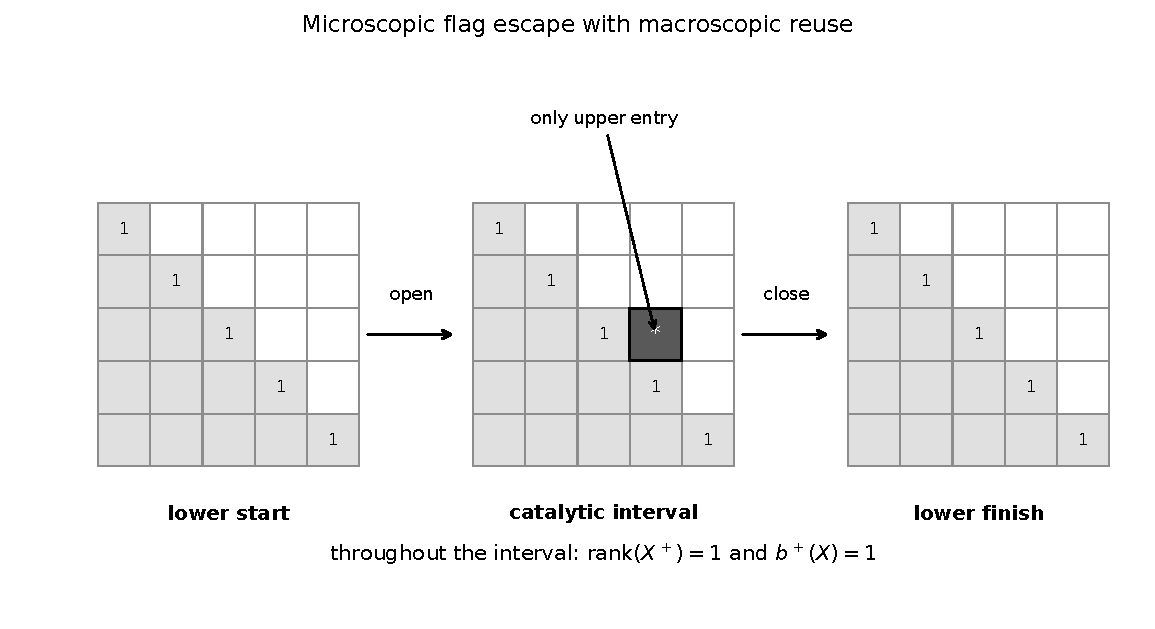
\includegraphics[width=.82\linewidth]{assets/g_microscopic_escape.pdf}
\caption{The snapshot circuit leaves the lower subgroup through one adjacent upper entry.  Throughout the excursion the strict upper part has rank one and bandwidth one, yet the accumulated saving grows linearly.}
\label{g:fig:microscopic-escape}
\end{figure}

\subsection{A weighted upper-gate metric}

A hardware or fault model may penalize an upper-directed interaction more heavily than a lower-directed one.  Fix $\lambda>0$.  If $w$ has $d(w)$ lower-directed gates and $u(w)$ upper-directed gates, put
\[
\operatorname{cost}_{\lambda}(w)=d(w)+\lambda u(w),
\]
and define
\[
\ellWeight{\lambda}(A)
=
\inf\{\operatorname{cost}_{\lambda}(w):[w]=A\}.
\]
At $\lambda=1$ this is the ordinary ambient length, while large $\lambda$ increasingly penalizes flag excursions.

\begin{proposition}[Fixed penalties do not suppress catalysis]\label{g:prop:weighted-catalysis}
For every snapshot target $A=A(u;s_1,\ldots,s_v)$ and every $\lambda>0$,
\[
\ellWeight{\lambda}(A)
\le
u+v+2\lambda.
\]
Consequently,
\[
\ellDown(A)-\ellWeight{\lambda}(A)
\ge
v-2\lambda.
\]
For the optimized connected family,
\[
\ellDown(A_n)-\ellWeight{\lambda}(A_n)
\ge
\left\lfloor\frac{n-1}{2}\right\rfloor-2\lambda.
\]
In particular, for every fixed finite $\lambda$, the weighted advantage grows linearly with $n$.
\end{proposition}

\begin{proof}
The displayed catalytic word contains $u+v$ lower-directed gates and two upper-directed gates, so its weighted cost is $u+v+2\lambda$.  Subtract this from the exact restricted value $u+2v$.  The optimized family again has $v=\lfloor(n-1)/2\rfloor$.
\end{proof}

\begin{remark}[Penalty threshold]
For the displayed realization of a snapshot target, catalysis beats the optimal lower-only cost whenever
\[
\lambda<\frac v2.
\]
The critical penalty therefore scales with the number of consumers, not with the dimension of the dirty workspace.
\end{remark}

\begin{figure}[t]
\centering
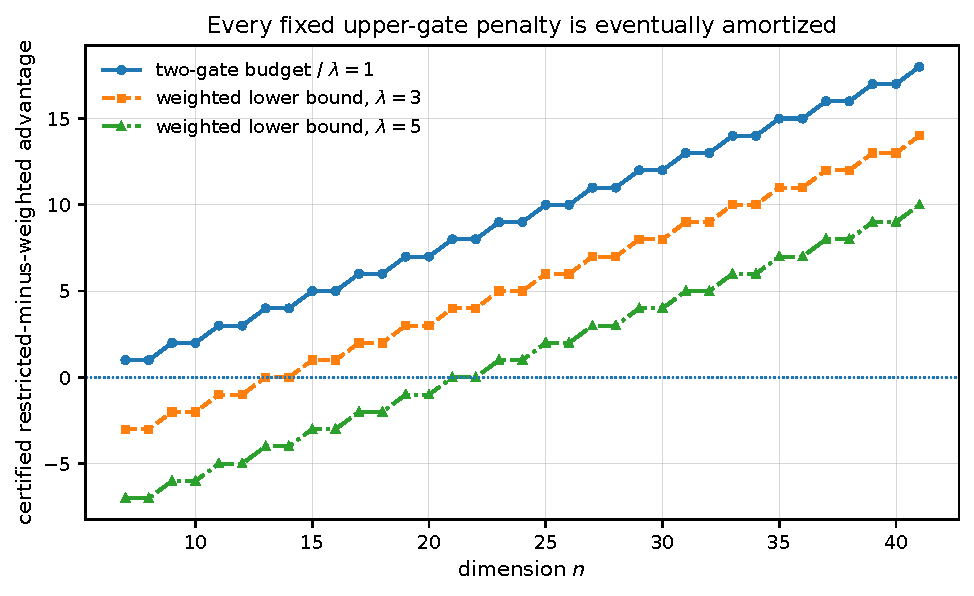
\includegraphics[width=.78\linewidth]{assets/g_weighted_catalysis.pdf}
\caption{Certified lower-minus-weighted advantage for the optimized connected family.  Every fixed upper-gate penalty is eventually amortized because the same matched excursion serves a growing number of output snapshots.}
\label{g:fig:weighted-catalysis}
\end{figure}

\begin{proof}[Proof of \cref{g:thm:resource-robustness}]
Combine \cref{g:prop:two-upper-linear,g:prop:weighted-catalysis}.
\end{proof}


\section{Algebraic rarity of catalytic defects}\label{g:sec:rarity}

The preceding sections construct highly structured targets with large defects.  This section proves the complementary statement that catalytic defects are nongeneric at every fixed dimension.  Fix a field $K$.  Algebraic dimensions and closures are taken after base change to an algebraic closure of $K$.  Put
\[
N=\dim \U_n=\binom n2,
\qquad
M=n(n-1).
\]

\subsection{Transvection product loci}

For a direction skeleton
\[
\sigma=((t_1,s_1),\ldots,(t_L,s_L)),
\qquad t_i\ne s_i,
\]
define the polynomial word map
\[
\Phi_\sigma:\Aff^L\longrightarrow\SL_n,
\qquad
(a_1,\ldots,a_L)
\longmapsto
(I+a_LE_{t_L,s_L})\cdots(I+a_1E_{t_1,s_1}).
\]
The coefficients are allowed to vanish, so a word of length at most $L$ can be padded to length $L$.  Let
\[
\mathcal R^*_{n,\le L}
=
\U_n\cap
\bigcup_{\sigma\in\{(t,s):t\ne s\}^L}
\operatorname{im}\Phi_\sigma
\]
be the ambient reachability locus, and define $\mathcal R^\downarrow_{n,\le L}$ analogously using only lower directions.

Equivalently, put
\[
X_*
=
\bigcup_{t\ne s}\{I+aE_{t,s}:a\in K\},
\qquad
X_\downarrow
=
\bigcup_{s<t}\{I+aE_{t,s}:a\in K\}.
\]
Then $\ellAll(A)$ and $\ellDown(A)$ are the corresponding transvection product lengths: the least $L$ for which $A\in X_*^L$ or $A\in X_\downarrow^L$.

\begin{proposition}[Dimension of bounded-length loci]\label{g:prop:reachability-dimension}
For every $L\ge0$, the sets $\mathcal R^*_{n,\le L}$ and $\mathcal R^\downarrow_{n,\le L}$ are constructible and
\[
\dim\overline{\mathcal R^*_{n,\le L}}
\le L,
\qquad
\dim\overline{\mathcal R^\downarrow_{n,\le L}}
\le L.
\]
\end{proposition}

\begin{proof}
There are finitely many direction skeletons of length $L$.  For each skeleton, $\Phi_\sigma$ is a morphism from an $L$-dimensional affine space.  Chevalley's theorem makes its image constructible, and the closure of the image has dimension at most $L$ \cite{g:Hartshorne1977}.  Finite unions preserve constructibility and the maximum dimension bound.  Intersecting with the closed subvariety $\U_n$ cannot increase dimension.
\end{proof}

The argument is an instance of a general parameter-counting principle.

\begin{proposition}[Dimension per gate]\label{g:prop:dimension-per-gate}
Let $G$ be an algebraic group, let $V\subseteq G$ be an irreducible subvariety of dimension $D$, and let $X\subseteq G$ be a finite union of locally closed subvarieties, each of dimension at most $r$, with the identity in $X$.  Write
\[
X^{(L)}
=
\{x_L\cdots x_1:x_1,\ldots,x_L\in X\}.
\]
Then
\[
\dim\overline{V\cap X^{(L)}}\le rL.
\]
In particular, if $rL<D$, a Zariski-generic point of $V$ has $X$-product length greater than $L$.
\end{proposition}

\begin{proof}
Every irreducible component of the Cartesian power $X^{\times L}$ has dimension at most $rL$.  Multiplication $G^L\to G$ is a morphism, so the closure of the image of each component has dimension at most $rL$.  There are finitely many components, and intersecting the resulting finite union with $V$ cannot increase dimension.  Since the identity belongs to $X$, products of length at most $L$ are already contained in $X^{(L)}$.
\end{proof}

For transvections, the discrete choice of direction contributes finitely many components and each component carries one scalar parameter.  Thus $r=1$.  Every element of $\U_n(K)$ has lower length at most $N$: process the strict lower entries in any root order compatible with elimination.  The dimension-per-gate bound shows that this worst-case value is generic.

\begin{theorem}[Generic rigidity]\label{g:thm:generic-rigidity}
Let $K$ be an infinite field.  There is a nonempty Zariski-open subvariety $\Omega_n\subseteq\U_n$, defined over $K$, such that $\Omega_n(K)$ is nonempty and
\[
\ellAll(A)=\ellDown(A)=N
\qquad(A\in\Omega_n(K)).
\]
The same statement holds with exact product length replaced by border product length.
\end{theorem}

\begin{proof}
After base change to an algebraic closure $\overline K$, \cref{g:prop:reachability-dimension} gives
\[
\dim\overline{\mathcal R^*_{n,\le N-1}}\le N-1<N=\dim\U_n.
\]
Because the word maps are defined over $K$, this proper closed set descends to a proper closed subset of $\U_n$ over $K$.  Its complement is a nonempty Zariski-open set $\Omega_n$.  Since $K$ is infinite and $\U_n\cong\Aff^N$, the set $\Omega_n(K)$ is nonempty and Zariski dense.  For any $A\in\Omega_n(K)$, one has $\ellAll(A)\ge N$.  The inequalities
\[
\ellAll(A)\le\ellDown(A)\le N
\]
force equality.  Replacing each image by its Zariski closure gives the border-length statement by the same argument.
\end{proof}

\subsection{Defect codimension}

For an algebraically closed field $K$ and $d\ge1$, define
\[
\mathcal D_{n,\ge d}
=
\{A\in\U_n(K):\DeltaDef(A)\ge d\}.
\]

\begin{theorem}[Defect--codimension bound]\label{g:thm:defect-codimension}
Let $K$ be algebraically closed.  For every $1\le d\le N$,
\[
\dim\overline{\mathcal D_{n,\ge d}}\le N-d.
\]
Equivalently,
\[
\codim_{\U_n}\overline{\mathcal D_{n,\ge d}}\ge d.
\]
More finely, on the stratum where $\ellDown(A)=L$ and $\DeltaDef(A)\ge d$, the closure has dimension at most $L-d$.
\end{theorem}

\begin{proof}
If $\DeltaDef(A)\ge d$, then
\[
\ellAll(A)
\le
\ellDown(A)-d
\le
N-d.
\]
Thus $\mathcal D_{n,\ge d}\subseteq\mathcal R^*_{n,\le N-d}$, and \cref{g:prop:reachability-dimension} gives the first assertion.  On the intrinsic-length-$L$ stratum one instead has $\ellAll(A)\le L-d$, proving the refinement.
\end{proof}

\begin{figure}[t]
\centering
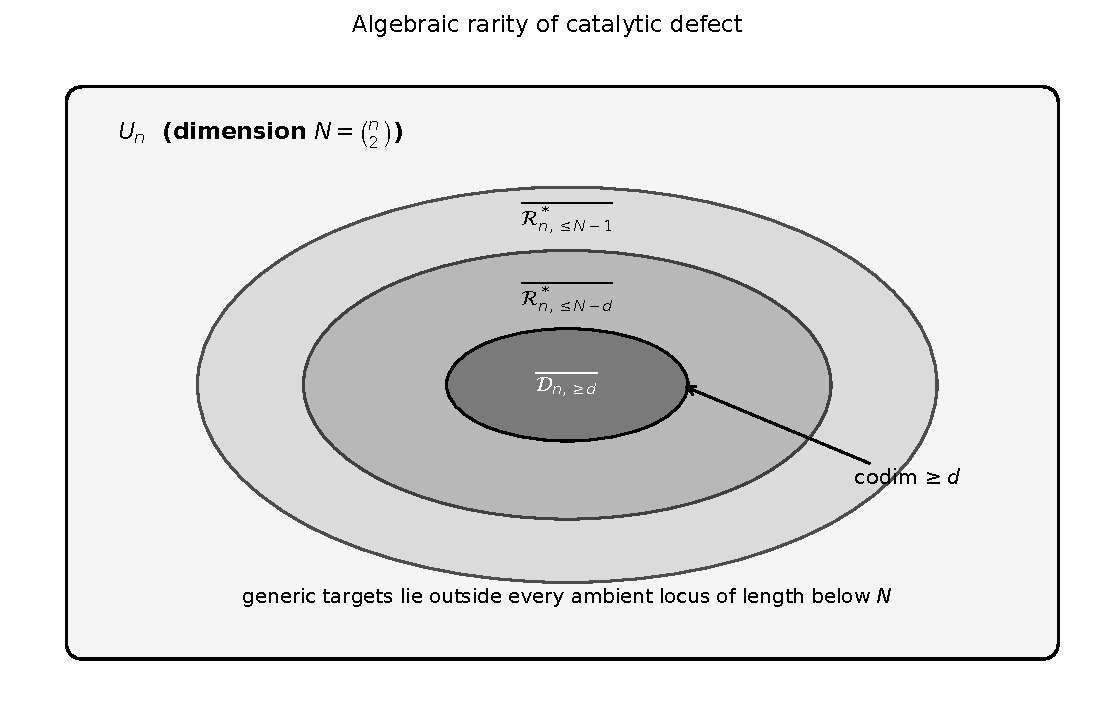
\includegraphics[width=.78\linewidth]{assets/g_defect_strata.pdf}
\caption{Bounded ambient product loci form nested algebraic strata inside $\U_n$.  A defect of size at least $d$ lies inside the ambient reachability locus of length $N-d$, whose closure has codimension at least $d$.}
\label{g:fig:defect-strata}
\end{figure}

\subsection{Finite-field sparsity}

The dimension argument has an elementary counting counterpart.  Allowing zero coefficients, a padded word of length $L$ is specified by $L$ choices among $M$ directed positions and $L$ coefficients in $\F_q$.  Consequently
\[
|\mathcal R^*_{n,\le L}(\F_q)|\le(Mq)^L.
\]

\begin{corollary}[Finite-field defect density]\label{g:cor:finite-field-density}
For $1\le d\le N$,
\[
\Prob_{A\in\U_n(\F_q)}[\DeltaDef(A)\ge d]
\le
\min\{1,M^{N-d}q^{-d}\}.
\]
In particular, for fixed $n$,
\[
\Prob[\DeltaDef(A)>0]=O_n(q^{-1}),
\qquad
\Exp[\DeltaDef(A)]=O_n(q^{-1})
\]
as $q\to\infty$.
\end{corollary}

\begin{proof}
The defect condition implies ambient length at most $N-d$, so the number of such targets is at most $(Mq)^{N-d}$.  Divide by
\[
|\U_n(\F_q)|=q^N.
\]
The expectation bound follows from
\[
\Exp[\DeltaDef]=\sum_{d=1}^{N}\Prob[\DeltaDef\ge d].
\]
\end{proof}

The same counting argument also gives
\[
\Prob_{A\in\U_n(\F_q)}[\ellAll(A)=\ellDown(A)=N]
\ge
1-M^{N-1}q^{-1},
\]
whenever the right side is positive.  Thus maximal ambient and intrinsic length is not only Zariski generic over infinite fields but asymptotically typical over growing finite fields at fixed dimension.

\subsection{Border catalysis}

For an algebraic generating set $X$, define the border product length
\[
\underline\ell_X(A)
=
\min\{L:A\in\overline{X^L}\}.
\]
This is analogous to the passage from tensor rank to border rank \cite{g:Landsberg2012}.  The generic value is still $N$ by \cref{g:thm:generic-rigidity}, but exact and border defects can differ on exceptional strata.  It is presently open whether the canonical atom $C$ belongs to the closure of the six-factor lower transvection locus.  A negative answer would show that its one-gate defect is stable under algebraic degeneration; a positive answer would exhibit a rank-versus-border-rank phenomenon inside reversible linear synthesis.

\begin{remark}[Rare but amplifiable]\label{g:rem:rare-amplifiable}
The codimension theorem and the tensor construction point in opposite directions without contradiction.  At each fixed $n$, a defect of size $d$ lies on a codimension-at-least-$d$ subset.  Carefully selected points on these thin strata can nevertheless be tensorized into families with $\Omega(n\log n)$ additive defect.  Catalytic compression is therefore algebraically rare but asymptotically amplifiable.
\end{remark}

\section{Recursive, block, and tensor amplification}\label{g:sec:amplification}

\subsection{Restricted block additivity}

The lower metric is exactly additive on contiguous block-diagonal targets.

\begin{proposition}[Block additivity]\label{g:prop:block-additivity}
Let $A_i\in\U_{n_i}(\F)$ for $1\le i\le k$.  Then
\[
\ellDown\bigl(\operatorname{diag}(A_1,\ldots,A_k)\bigr)
=
\sum_{i=1}^k\ellDown(A_i).
\]
\end{proposition}

\begin{proof}
The upper bound follows by running optimal lower circuits independently inside the blocks.

For the lower bound, view an element of $\U_{n_1+\cdots+n_k}(\F)$ as a lower block-triangular matrix and project to its diagonal blocks:
\[
\pi(X)=(X_{11},\ldots,X_{kk}).
\]
Because diagonal blocks multiply independently in a lower block-triangular product, $\pi$ is a homomorphism.  A lower transvection internal to one block projects to one generator in that factor, while a crossing transvection projects to the identity in every factor.  If $m_i$ gates survive in factor $i$, then the total word length is at least
\[
\sum_i m_i
\ge
\sum_i\ellDown(A_i).
\]
\end{proof}

The ambient metric is subadditive:
\[
\ellAll\bigl(\operatorname{diag}(A_1,\ldots,A_k)\bigr)
\le
\sum_i\ellAll(A_i).
\]
Cross-block ambient workspace can only improve this upper bound.

\begin{corollary}[Block-sum amplification]\label{g:cor:linear-gap}
For every field and every $n\ge6$, there is an $A_n\in\U_n(\F)$ with
\[
\ellDown(A_n)-\ellAll(A_n)
\ge
\left\lfloor\frac n6\right\rfloor.
\]
For $n=6k$, the target $C^{\oplus k}$ satisfies
\[
\ellDown(C^{\oplus k})=7k,
\qquad
\ellAll(C^{\oplus k})\le6k.
\]
\end{corollary}

\begin{proof}
For $n=6k+r$, take $C^{\oplus k}\oplus I_r$ and apply block additivity together with $k$ copies of the ambient six-gate word.
\end{proof}

\begin{figure}[t]
\centering
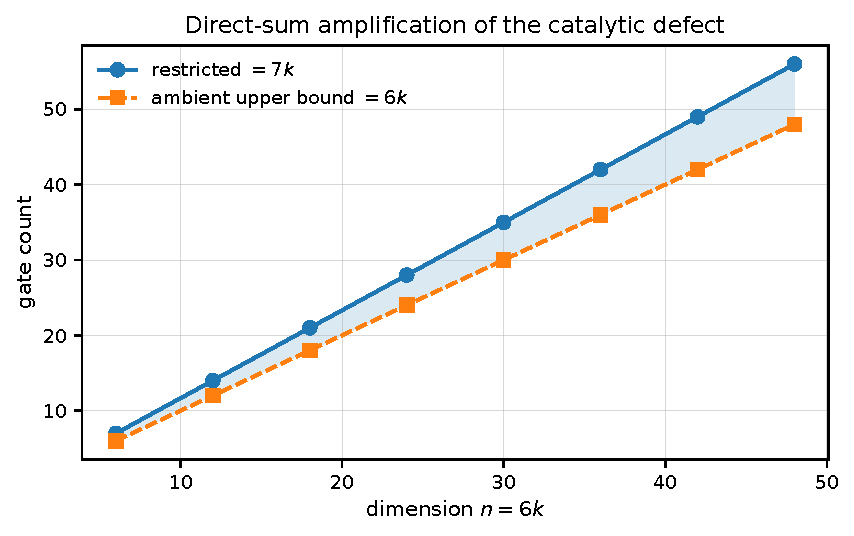
\includegraphics[width=.68\linewidth]{assets/g_direct_sum_amplification.pdf}
\caption{Block-sum amplification.  The restricted length is exactly $7k$, while the displayed ambient construction has length $6k$.}
\label{g:fig:direct-sum}
\end{figure}

\subsection{A recursive zeta-shaped lift}

For $A\in\U_m(\F)$, define
\begin{equation}\label{g:eq:zeta-lift}
\mathcal Z(A)
=
\begin{pmatrix}
A&0\\
A&A
\end{pmatrix}
\in\U_{2m}(\F).
\end{equation}

\begin{proposition}[Exact restricted lift]\label{g:prop:zeta-lift}
For every $A\in\U_m(\F)$,
\[
\ellDown(\mathcal Z(A))=2\ellDown(A)+m,
\]
and
\[
\ellAll(\mathcal Z(A))\le2\ellAll(A)+m.
\]
Consequently,
\[
\DeltaDef(\mathcal Z(A))\ge2\DeltaDef(A).
\]
\end{proposition}

\begin{proof}
The construction first realizes $\operatorname{diag}(A,A)$ and then applies the $m$ root-cross gates that add top row $i$ into bottom row $i$.

For the lower bound, write a circuit state in $m\times m$ blocks as
\[
X=
\begin{pmatrix}
P&0\\
Q&R
\end{pmatrix}.
\]
Projection to the two diagonal blocks forces at least $2\ellDown(A)$ internal gates.  A top-internal gate leaves $Q$ unchanged.  A bottom-internal gate performs an invertible row operation on $Q$ and preserves its rank.  A root-cross gate changes $Q$ by one rank-one row contribution, so it can increase $\rank Q$ by at most one.  The final cross block is $A$, of rank $m$, hence at least $m$ root-cross gates are necessary.
\end{proof}

Let $A^{[0]}=A$ and $A^{[r+1]}=\mathcal Z(A^{[r]})$.  If $A$ has size $m$, restricted length $a$, and ambient length $b$, then
\begin{equation}\label{g:eq:zeta-iterate}
\ellDown(A^{[r]})
=
2^r a+r m2^{r-1},
\end{equation}
and
\begin{equation}\label{g:eq:zeta-iterate-ambient}
\ellAll(A^{[r]})
\le
2^r b+r m2^{r-1}.
\end{equation}
Thus
\[
\DeltaDef(A^{[r]})\ge2^r\DeltaDef(A).
\]
For the canonical atom $C$, the first values are
\begin{center}
\begin{tabular}{@{}rrrrr@{}}
\toprule
$r$&dimension&restricted exact&ambient upper bound&certified gap\\
\midrule
$0$&$6$&$7$&$6$&$1$\\
$1$&$12$&$20$&$18$&$2$\\
$2$&$24$&$52$&$48$&$4$\\
$3$&$48$&$128$&$120$&$8$\\
$4$&$96$&$304$&$288$&$16$\\
\bottomrule
\end{tabular}
\end{center}
This gives arbitrarily deep exact recursion with identical diagonal children and a full-rank cross block while preserving a positive defect.

\begin{figure}[t]
\centering
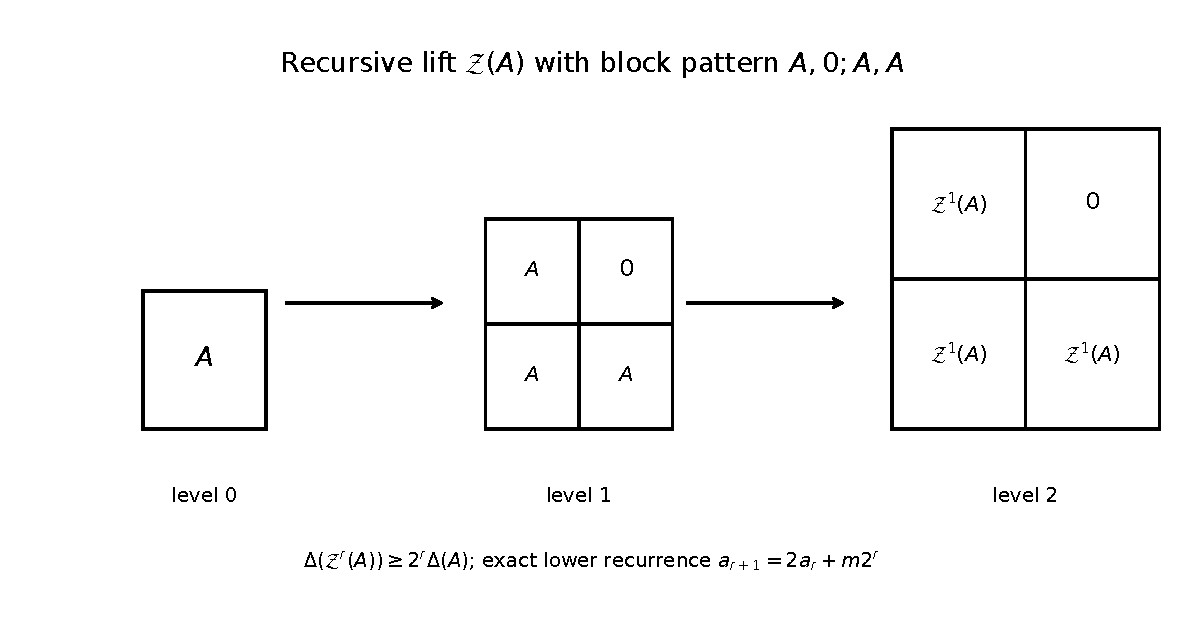
\includegraphics[width=.88\linewidth]{assets/g_recursive_zeta_lift.pdf}
\caption{The recursive lift has the same outer shape as a Boolean zeta recursion.  A finite defect at the leaf is doubled at every lift.}
\label{g:fig:zeta-lift}
\end{figure}

\subsection{Tensor products of tree-tight targets}

The tensor operation gives the stronger asymptotic amplification.

\begin{theorem}[Exact restricted tensor rule]\label{g:thm:tensor-rule}
Let $A\in\U_m(\F)$ and $B\in\U_n(\F)$ be tree tight.  Then $A\otimes B$ is tree tight and
\begin{equation}\label{g:eq:tensor-lower}
\ellDown(A\otimes B)
=
n\ellDown(A)+m\ellDown(B).
\end{equation}
Moreover,
\begin{equation}\label{g:eq:tensor-ambient}
\ellAll(A\otimes B)
\le
n\ellAll(A)+m\ellAll(B),
\end{equation}
so
\begin{equation}\label{g:eq:tensor-defect}
\DeltaDef(A\otimes B)
\ge
n\DeltaDef(A)+m\DeltaDef(B).
\end{equation}
\end{theorem}

\begin{proof}
Use lexicographic order on the $mn$ coordinates.  Substitute a copy of a certificate tree for $B$ at every leaf of a certificate tree for $A$.  At an outer node, the cross block is
\[
A[R,L]\otimes B,
\]
whose rank is $n\rank A[R,L]$ because $B$ is invertible.  The outer nodes therefore contribute $n\ellDown(A)$.  The $m$ diagonal copies of the inner tree contribute $m\ellDown(B)$.  This proves the lower bound.

For the matching lower construction, first realize $I_m\otimes B$ using $m$ copies of a circuit for $B$.  Then realize $A\otimes I_n$.  Each gate of a circuit for $A$ lifts to $n$ coordinatewise gates.  Since
\[
(A\otimes I_n)(I_m\otimes B)=A\otimes B,
\]
the cost is the right side of \cref{g:eq:tensor-lower}.  The same construction with ambient circuits proves \cref{g:eq:tensor-ambient}.
\end{proof}

If $A$ is tree tight of dimension $m$, with restricted length $a$ and an ambient construction of length $b$, then
\begin{equation}\label{g:eq:tensor-power-lower}
\ellDown(A^{\otimes r})
=
r m^{r-1}a,
\end{equation}
and
\begin{equation}\label{g:eq:tensor-power-upper}
\ellAll(A^{\otimes r})
\le
r m^{r-1}b.
\end{equation}
A positive one-copy defect therefore becomes an order-$N\log N$ defect at dimension $N=m^r$.

\begin{proof}[Proof of \cref{g:thm:tensor-main}]
Apply \cref{g:thm:tensor-rule} repeatedly to the tree-tight snapshot target $A=A(u;s_1,\ldots,s_v)$, for which
\[
a=u+2v,
\qquad
b=u+v+2=m.
\]
Then
\[
\ellDown(A^{\otimes r})
-
\ellAll(A^{\otimes r})
\ge
r m^{r-1}(v-2).
\]
Since $N=m^r$ and $r=\log_2N/\log_2m$, this is
\[
\frac{v-2}{m\log_2m}N\log_2N.
\]
\end{proof}

Within the snapshot family, the best coefficient is obtained by the twenty-one-dimensional seed
\[
A_{21}=A(9;0,1,\ldots,9),
\]
for which
\[
\ellDown(A_{21})=29,
\qquad
\ellAll(A_{21})\le21,
\qquad
\DeltaDef(A_{21})\ge8.
\]

\begin{proposition}[Optimal snapshot seed for tensor rate]\label{g:prop:optimal-snapshot-seed}
Among all snapshot targets, the coefficient
\[
\frac{v-2}{m\log_2m},
\qquad m=u+v+2,
\]
is maximized at
\[
(m,u,v)=(21,9,10).
\]
\end{proposition}

\begin{proof}
For fixed $m$, maximize $v$ subject to $v\le u+1$ and $u+v+2=m$.  Thus
\[
v=\left\lfloor\frac{m-1}{2}\right\rfloor.
\]
If $m$ is even and at least eight, its coefficient is strictly smaller than that of $m-1$, because the numerator is the same while
\[
(m-1)\log(m-1)<m\log m.
\]
It therefore suffices to consider odd $m$.  Apart from the constant change of logarithm base, the odd-dimensional envelope is
\[
f(x)=\frac{x-5}{2x\log x}.
\]
Its derivative has the sign of
\[
5(1+\log x)-x.
\]
For $x>5$ this expression crosses zero exactly once, between $19$ and $21$.  Direct comparison gives $f(21)>f(19)$, after which the envelope decreases.  Hence the unique integer maximizer is $m=21$.
\end{proof}

The first tensor powers are
\begin{center}
\begin{tabular}{@{}rrrrr@{}}
\toprule
$r$&dimension $21^r$&restricted exact&ambient upper bound&certified gap\\
\midrule
$1$&$21$&$29$&$21$&$8$\\
$2$&$441$&$1218$&$882$&$336$\\
$3$&$9261$&$38367$&$27783$&$10584$\\
$4$&$194481$&$1074276$&$777924$&$296352$\\
\bottomrule
\end{tabular}
\end{center}

\begin{figure}[t]
\centering
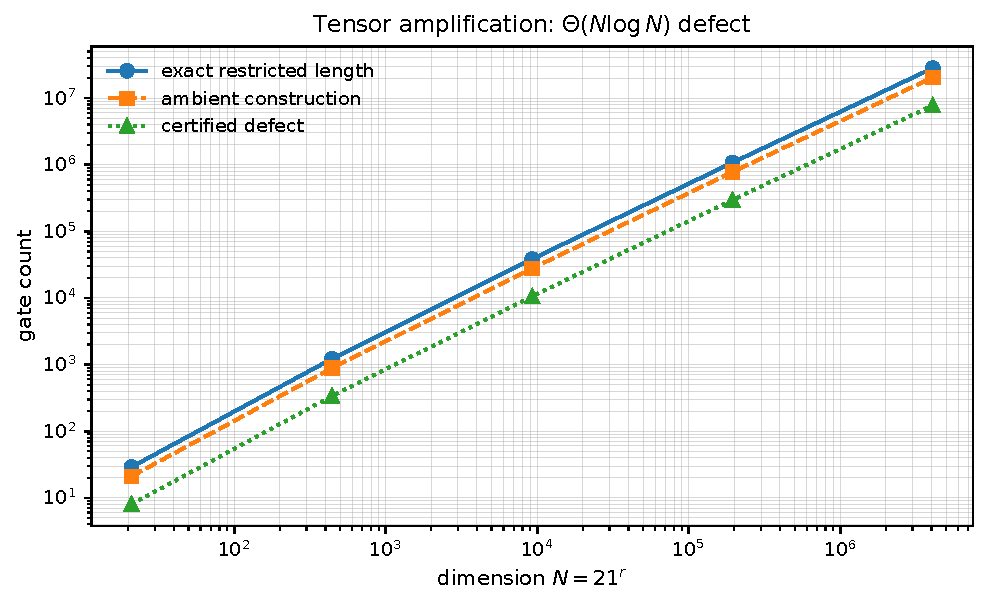
\includegraphics[width=.74\linewidth]{assets/g_tensor_amplification.pdf}
\caption{Tensor powers of the twenty-one-dimensional snapshot seed.  Both displayed circuit sizes are of order $N\log N$, and their difference has a positive $N\log N$ coefficient.}
\label{g:fig:tensor-amplification}
\end{figure}

\subsection{Stable tensor capacity and activation}\label{g:subsec:stable-tensor}

The tensor inequality also defines a regularized ambient invariant.  Let $A\in\U_m(\F)$ and put
\[
b_r(A)
=
\frac{\ellAll(A^{\otimes r})}{m^{r-1}}.
\]
Applying \cref{g:eq:tensor-ambient} to $A^{\otimes r}\otimes A^{\otimes s}$ gives
\[
b_{r+s}(A)\le b_r(A)+b_s(A).
\]

\begin{proposition}[Stable tensor length]\label{g:prop:stable-tensor-length}
The limit
\[
\tau_*(A)
=
\lim_{r\to\infty}
\frac{\ellAll(A^{\otimes r})}{r m^{r-1}}
=
\inf_{r\ge1}
\frac{\ellAll(A^{\otimes r})}{r m^{r-1}}
\]
exists.  If $A$ is tree tight, then the stable catalytic capacity
\[
\kappa_\otimes(A)
=
\ellDown(A)-\tau_*(A)
\]
satisfies
\[
\kappa_\otimes(A)\ge\DeltaDef(A).
\]
\end{proposition}

\begin{proof}
The sequence $b_r(A)$ is subadditive, so Fekete's lemma gives the displayed limit.  Since the one-copy lifted construction implies $\tau_*(A)\le\ellAll(A)$, one has
\[
\kappa_\otimes(A)
\ge
\ellDown(A)-\ellAll(A)
=
\DeltaDef(A).
\]
For a tree-tight target, \cref{g:eq:tensor-power-lower} identifies $\ellDown(A)$ with its exact normalized restricted tensor cost.
\end{proof}

For the twenty-one-dimensional seed $A_{21}$,
\[
\kappa_\otimes(A_{21})\ge8.
\]
This regularization introduces a new possibility: a target may have $\DeltaDef(A)=0$ but $\kappa_\otimes(A)>0$.  In that case one copy is rigid while many tensor copies admit a collective shortcut.  We call this \emph{tensor activation}.

\subsection{Extremal consequences}

Define
\[
D_n(\F)
=
\sup_{A\in\U_n(\F)}
\bigl(\ellDown(A)-\ellAll(A)\bigr).
\]
For finite fields the supremum is a maximum.  The tensor family gives the following explicit all-dimension bound.

\begin{proof}[Proof of \cref{g:cor:nlogn-gap}]
Let $m=21$ and write
\[
n=\sum_{j=0}^{r}d_jm^j,
\qquad
0\le d_j<m.
\]
Take the block sum of $d_j$ copies of $A_{21}^{\otimes j}$ for every $j$, with the convention $A_{21}^{\otimes0}=I_1$.  Block additivity and the tensor estimate give
\[
D_n(\F)
\ge
\frac{8}{21}
\sum_{j=0}^{r}j d_j21^j.
\]
Put $S=\sum_j j d_j21^j$.  Since $r=\lfloor\log_{21}n\rfloor$,
\[
r n-S
=
\sum_{j<r}(r-j)d_j21^j
\le
20\sum_{h\ge1}h21^{r-h}
\le
\frac{21^{r+1}}{20}
\le
\frac{21}{20}n.
\]
Also $r\ge\log_{21}n-1$.  Therefore
\[
S\ge n\log_{21}n-\frac{41}{20}n.
\]
Multiplying by $8/21$ yields
\[
D_n(\F)
\ge
\frac{8}{21\log_2 21}n\log_2n
-
\frac{82}{105}n.
\]
\end{proof}

Numerically,
\[
\frac{8}{21\log_2 21}
=0.0867315\ldots.
\]
The elementary bottom-to-top construction gives
\[
D_n(\F)\le\frac{n(n-1)}2.
\]
Thus the current general range is
\begin{equation}\label{g:eq:defect-range}
0.0867315\,n\log_2n-O(n)
\le
D_n(\F)
\le
\frac{n(n-1)}2.
\end{equation}

\section{Discussion and open problems}\label{g:sec:discussion}

\subsection{What the threshold and higher families establish}

The six-row atom proves that an optimal circuit for a lower-unitriangular target need not remain in the lower-unitriangular subgroup.  The exact binary classification shows that this first failure is rigid: it occurs for exactly twenty targets, every defect is $(7,6)$, and every target is generated by the same three-cross, one-phase mechanism.

The higher-dimensional results change the scale of the phenomenon.  The connected snapshot family shows that exactly two upper-directed gates can support a defect linear in dimension, and that the advantage persists under every fixed finite penalty on those gates.  The recursive lift shows that a defective leaf survives arbitrarily many identical full-rank dyadic levels.  Tensor products then turn any tree-tight positive-defect atom into an order-$N\log N$ additive separation.  Thus the defect is not a finite anomaly and not merely linear in the worst case.  At the same time, generic rigidity and the defect--codimension theorem show that large defects require correspondingly special algebraic conditions.  The central synthesis is therefore not ubiquity but amplification: thin exceptional strata can control large structured families.

\subsection{Relation to ordinary CNOT synthesis}

Exact CNOT synthesis usually minimizes $\ellAll$ on all of $\GL_n(\F_2)$.  The present problem fixes a structured target class and compares the ambient optimum with a structure-preserving optimum.  Recent exact methods explore the full Cayley graph using symmetries, bidirectional search, A* methods, SAT, and related techniques \cite{g:ChristensenEtAl2025,g:WebsterEtAl2025,g:ShaikVanDePol2025}.  The right-coset computation in this paper is tailored to a subgroup comparison, while the higher-dimensional exact audits use direct bidirectional balls for selected targets.

The 2026 NP-completeness result for all-to-all CNOT distance shows that cancellation and unrestricted parity reuse must be handled in full generality \cite{g:AcuavivaEtAl2026}.  The present constructions isolate explicit reusable-carrier mechanisms under an ordered restriction.  They do not resolve ambient synthesis complexity.

\subsection{Open directions}

\begin{question}[Universal six-dimensional threshold]
Is six the first defective dimension over every field, or even over every nonzero commutative ring?  The atom gives a universal defective target in dimension six.  Exact no-defect searches below six are proved here for $\F_2$ and $\F_3$.
\end{question}

\begin{question}[Geometry of the defect locus]
For fixed $n$ and $d$, determine the irreducible components and exact dimension of $\overline{\mathcal D_{n,\ge d}}$.  When is the lower bound $\codim\ge d$ sharp?
\end{question}

\begin{question}[Border catalysis]
Does the canonical atom have lower border product length six or seven?  More generally, when can exact catalytic defects disappear under algebraic degeneration?
\end{question}

\begin{question}[Correct growth of the maximum defect]
Is $D_n(\F)$ of order $n\log n$, or can interacting catalysts produce a larger power of $n$?  The current bounds are
\[
\Omega(n\log n)
\le
D_n(\F)
\le
O(n^2).
\]
\end{question}

\begin{question}[Multiplicative distortion]
Is
\[
\sup_{n,A\in\U_n(\F)}
\frac{\ellDown(A)}{\ellAll(A)}
\]
bounded?  The connected snapshot family gives an asymptotic lower bound of $3/2$.  Exceeding $3/2$ appears to require a mechanism beyond one clean carrier exporting independent snapshots.
\end{question}

\begin{question}[Exact ambient complexity of snapshot targets]
For which phase sets is the ambient construction of length $u+v+2$ optimal?  It is exact for the displayed binary targets in dimensions seven, eight, and nine, but the general ambient optimum remains open.
\end{question}

\begin{question}[Tensor synergy and activation]
Can $A\otimes B$ admit an ambient circuit shorter than the lifted bound
\[
n\ellAll(A)+m\ellAll(B)?
\]
Such synergy would only increase the defect, but understanding it is necessary for exact tensor complexity.  Does there exist a tree-tight target with $\DeltaDef(A)=0$ but $\kappa_\otimes(A)>0$?
\end{question}

\begin{question}[Higher catalytic normal forms]
Can interacting or crossing catalytic excursions produce asymptotic behavior impossible for a single clean carrier?  A useful classification would separate laminar, crossing, and singular flag excursions.
\end{question}

\begin{question}[Two-gate multiplicative ceiling]
Among targets realizable with at most two upper-directed gates, is the asymptotic multiplicative distortion at most $3/2$?  The snapshot family reaches this value from below, but the present paper proves no matching upper bound.
\end{question}

\begin{question}[Matroidal classification]
Which regular matroids admit a flagged realization whose shortest ambient state tour is strictly shorter than every flag-compatible lift?  The first atom is the graphic matroid $M(K_4)$ with designated source, carrier, and output roles.
\end{question}

\begin{question}[Weighted phase transition]
For a fixed target family, determine the exact critical penalty $\lambda_c$ at which a flag excursion ceases to improve the optimal weighted cost.  The snapshot construction proves only the lower bound $\lambda_c\ge v/2$ for its displayed carrier word.
\end{question}

\begin{question}[Other root systems]
Let $G$ be a split reductive group with unipotent radical $U$.  Compare word length in positive root subgroups with ambient word length using all root subgroups.  Which root systems admit a catalytic defect, and what is the first rank?
\end{question}

\begin{question}[Certificate extraction]
Can exact ambient lower bounds for large structured targets be accompanied by short human-readable certificates rather than exhaustive balls?  The interval-tree method completely handles the restricted side, while the ambient side still lacks an equally general certificate.
\end{question}


\section{The twenty binary dimension-six defects}\label{g:app:twenty}

A lower-unitriangular binary matrix is encoded by reading the strict lower entries row by row:
\[
(1,0),
(2,0),(2,1),
\ldots,
(5,0),\ldots,(5,4).
\]
The resulting fifteen-bit integer is denoted by $\operatorname{code}(A)$.  A row is displayed as the integer whose binary expansion is its support vector.  \Cref{g:tab:twenty} lists all defects.  Every row has $\ellDown=7$ and $\ellAll=6$.

\begin{longtable}{@{}rllllll@{}}
\caption{The twenty defective matrices in $\U_6(\F_2)$.}\label{g:tab:twenty}\\
\toprule
code&$R_0$&$R_1$&$R_2$&$R_3$&$R_4$&$R_5$\\
\midrule
\endfirsthead
\toprule
code&$R_0$&$R_1$&$R_2$&$R_3$&$R_4$&$R_5$\\
\midrule
\endhead
6585&1&3&4&15&22&38\\
6641&1&3&4&14&23&38\\
6649&1&3&4&15&23&38\\
7601&1&3&4&14&22&39\\
7609&1&3&4&15&22&39\\
7665&1&3&4&14&23&39\\
10014&1&2&7&11&28&41\\
11038&1&2&7&11&28&42\\
12894&1&2&7&11&25&44\\
12958&1&2&7&11&26&44\\
13142&1&2&7&10&29&44\\
13198&1&2&7&9&30&44\\
14102&1&2&7&10&28&45\\
15118&1&2&7&9&28&46\\
17912&1&2&4&15&23&49\\
18936&1&2&4&15&23&50\\
19960&1&2&4&15&23&51\\
20984&1&2&4&15&23&52\\
22008&1&2&4&15&23&53\\
23032&1&2&4&15&23&54\\
\bottomrule
\end{longtable}

For example, the canonical target has row encoding
\[
(1,3,4,14,23,39)
\]
and code $7601$.

\section{Search algorithms and correctness}\label{g:app:algorithms}

\subsection{Restricted search}

For $\F_2$, each lower-unitriangular matrix is stored as a bit string.  Standard breadth-first search gives exact distance because every edge has unit weight.  The algorithm terminates after visiting all states.

\begin{algorithm}[Restricted breadth-first search]
Initialize $d[I]=0$ and a queue containing $I$.  Repeatedly remove $X$ from the queue.  For every lower transvection $s\to t$, form $Y=\tau_{t,s}(1)X$.  If $Y$ has not been visited, set $d[Y]=d[X]+1$ and append $Y$.  Continue until the queue is empty.
\end{algorithm}

\subsection{Right-coset key}

For an invertible binary matrix $A$, let $c_j$ be column $j$.  Starting at $j=n-1$ and moving left, reduce $c_j$ by the already canonicalized columns $c_{j+1},\ldots,c_{n-1}$, using their pivot coordinates.  The resulting ordered reduced columns form the key $\kappa(A)$.

\begin{lemma}
For $A,B\in\GL_n(\F_2)$,
\[
\kappa(A)=\kappa(B)
\quad\Longleftrightarrow\quad
AU_n=BU_n.
\]
\end{lemma}

\begin{proof}
Right multiplication by $U\in\U_n$ replaces column $j$ by itself plus a combination of columns with index greater than $j$.  Right-to-left reduction is therefore unchanged on a right coset.  Conversely, equal reduced columns imply that the original column frames differ by a unique lower-unitriangular column transformation, so $A=BU$ for some $U\in\U_n$.
\end{proof}

\subsection{Ambient search}

\begin{algorithm}[Radius-four right-coset meet in the middle]
Compute the exact radius-four ball $B_4$ in $\GL_6(\F_2)$.  Bucket its elements by $\kappa$.  For each bucket and every ordered pair $(b,a)$ in that bucket, compute $u=b^{-1}a\in\U_6$ and update
\[
d_*(u)\leftarrow
\min\bigl(d_*(u),d(b)+d(a)\bigr).
\]
\end{algorithm}

Correctness is \cref{g:lem:mitm-complete}.  The computation also checks that every generated pair lies in $\U_6$ and that every one of the $32768$ targets receives a finite distance.

\subsection{Higher-dimensional bidirectional audits}

For the targets $H_7,H_8,H_9$ of \cref{g:thm:higher-exact}, the program \texttt{small\_snapshot\_exact.cpp} constructs exact ambient balls from the identity and from the target.  If radius-$r$ and radius-$s$ balls are disjoint, symmetry of the generating set rules out every word of length at most $r+s$.  The tested splits are $3+3$, $3+4$, and $4+4$, respectively.  The source stores matrices in one 128-bit word and uses exact row-addition transitions; no probabilistic or floating-point step occurs.

\subsection{Symbolic higher-family checks}

The program \texttt{higher\_family\_tests.py} generates the snapshot targets over $\F_2$, $\F_3$, and $\F_5$, evaluates both displayed circuits, computes the interval-tree potentials, audits a tensor certificate for the seven-dimensional seed, verifies the recursive cross rank, and reproduces the twenty-one-dimensional rate optimization.

\subsection{Further generalization audits}

The program \texttt{further\_generalization\_tests.py} verifies the universal circuits over $\mathbb Z/4\mathbb Z$, $\mathbb Z/6\mathbb Z$, and $\mathbb Z/8\mathbb Z$, audits the rank-one bandwidth-one excursion, checks the finite-field counting bounds symbolically, and verifies the stable tensor subadditivity identities.

\subsection{Motif comparison}

The motif program independently loops over the three adjacent catalyst positions, the phase orientation, the phase leaf, and every nonempty proper before/after subset.  It evaluates each six-gate word from the identity and stores its target.  The resulting set has size twenty.  Exact comparison with the twenty census defects returns equality.

\section{Reproducibility ledger}\label{g:app:reproducibility}

The ancillary directory \texttt{supplement/} contains portable source, frozen expected outputs, and a one-command driver:
\begin{verbatim}
cd supplement
./run_all.sh
\end{verbatim}
The driver compiles every C++ search, executes the Python motif, higher-family, matroid, and weighted-resource checks, and compares all generated outputs byte for byte with the frozen records.  The supplement README gives the individual commands and the role of every program.  A SHA-256 manifest covers every included source and expected-output file.

\section*{Acknowledgement of computational status}

All theorem statements are labeled by proof type in the body.  The universal ring-valued atom, Schreier-holonomy interpretation, regular-matroid identification, interval-tree family, bounded, weighted, and microscopic resource theorems, algebraic-rarity bounds, block additivity, recursive lift, tensor rule, stable tensor limit, and asymptotic amplification are proved symbolically.  The first-threshold classification, finite censuses, and exact ambient values in dimensions seven through nine are computer assisted, with complete search-space coverage justified in \cref{g:app:algorithms}.

\section*{Data and code availability}

The source archive accompanying this paper contains the complete LaTeX source, all vector figures, every C++ and Python verification program, frozen expected outputs, and SHA-256 manifests.  The command
\begin{verbatim}
cd supplement
./run_all.sh
\end{verbatim}
rebuilds the finite searches and symbolic audits and compares every output byte for byte with its frozen record.  No randomized or floating-point decision enters a theorem certificate.


\chapter{Quantum and reversible gate families}
\section{Qudit SUM gates and ring-valued linear logic}\label{g:ch:qudit-sum}
\index{qudit SUM gate}
\index{controlled addition}
\index{ring universality}


\subsection{From transvections to quantum gates}
Let $d\ge2$.  On $n$ qudits with computational basis labeled by $\Z_d^n$, define the scaled SUM gate
\[
\SUM^{(a)}_{s\to t}
\ket{x_0,\ldots,x_{n-1}}
=
\ket{x_0,\ldots,x_t+a x_s,\ldots,x_{n-1}},
\qquad a\in\Z_d.
\]
It is a permutation unitary.  Its action on basis labels is the row transvection
\[
I+aE_{t,s}.
\]
For $d=2$ and $a=1$, it is CNOT.  For prime $d$, these gates lie in the standard qudit Clifford group.  For composite $d$, they remain exact reversible modular-addition gates.

\begin{provedbox}
The universal six-row atom in the core chapter is valid over every nonzero commutative ring with identity.  Taking $R=\Z_d$ gives a six-qudit target with restricted directed-SUM length seven and ambient all-direction SUM length six for every $d\ge2$.
\end{provedbox}

\subsection{The universal six-qudit circuit}
Use the coordinate names
\[
x,p,q,t_0,t_1,t_2.
\]
The target acts on basis labels by
\begin{align*}
p&\mapsto p+x,\\
t_0&\mapsto t_0+p+q,\\
t_1&\mapsto t_1+x+p+q,\\
t_2&\mapsto t_2+x+p+q,
\end{align*}
with $x$ and $q$ unchanged.  An ambient word is
\[
\SUM_{q\to p},
\quad
\SUM_{p\to t_0},
\quad
\SUM_{x\to p},
\quad
\SUM_{p\to t_1},
\quad
\SUM_{p\to t_2},
\quad
\SUM^{(-1)}_{q\to p}.
\]
The first gate adds the dirty $q$ component to $p$.  The middle gates export two different carrier states.  The final inverse gate restores $p$.

\begin{figure}[ht]
\centering
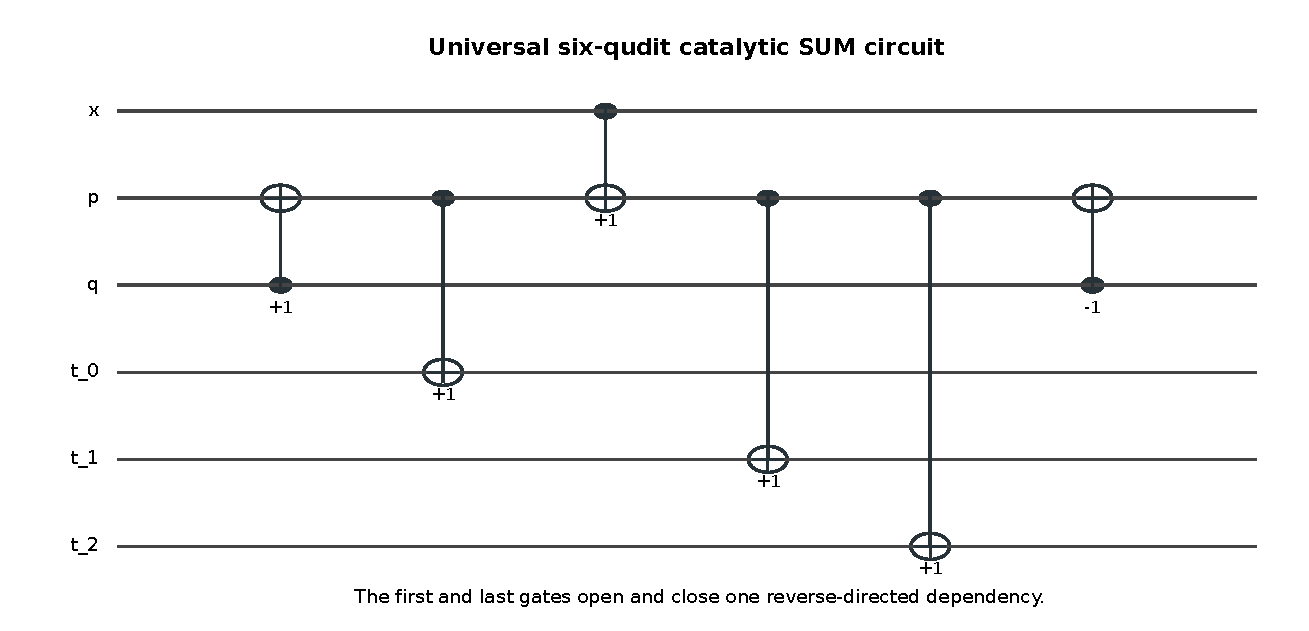
\includegraphics[width=.96\textwidth]{assets/g_qudit_sum_circuit.pdf}
\caption{The universal six-qudit catalytic circuit.  Coefficients are interpreted modulo $d$.}
\label{g:fig:qudit-sum}
\end{figure}

A lower-only word needs seven gates.  The exact proof is coefficient-domain independent because it uses pivot support and the number of distinct carrier states rather than division.

\subsection{Connected higher-dimensional qudit families}
The snapshot target $A(u;s_1,\ldots,s_v)$ from the core chapter is defined over any coefficient ring for which the displayed additions make sense.  Over $\Z_d$, it becomes a modular SUM circuit.  Its explicit ambient word uses exactly two reverse-directed SUM gates and has length
\[
u+v+2.
\]
The interval-tree proof of exact restricted length is most transparent over fields, but the displayed upper-bound and resource-amortization mechanism remain valid over every $\Z_d$.

For a field $\F_q$, the exact formula is
\[
\ellDown(A)=u+2v,
\qquad
\ellAll(A)\le u+v+2,
\]
so
\[
\Delta(A)\ge v-2.
\]
The connected family has asymptotic ratio approaching $3/2$.

\subsection{Weighted physical costs}
Suppose forward SUM gates cost one and reverse-directed SUM gates cost $\lambda$.  The displayed word has weighted cost
\[
u+v+2\lambda,
\]
while the restricted construction costs $u+2v$.  Hence the gain is at least
\[
v-2\lambda.
\]
This formula can be combined with hardware calibration.  If reverse orientation requires echo pulses or routing, the catalyst remains useful when the number of exported snapshots exceeds twice the effective penalty.

\begin{boundarybox}
A gate-count saving does not imply a lower physical error or depth.  Device-specific conclusions require a cost vector containing duration, infidelity, crosstalk, and routing.  The algebraic theorem identifies candidate rewrites and the exact break-even inequality.
\end{boundarybox}

\subsection{Pauli action for prime qudits}
For odd prime $d$, let $X$ and $Z$ denote generalized Pauli operators.  The SUM gate acts by
\begin{align*}
X_s&\mapsto X_sX_t^a,
&
X_t&\mapsto X_t,\\
Z_s&\mapsto Z_s,
&
Z_t&\mapsto Z_s^{-a}Z_t.
\end{align*}
Thus the modular linear action embeds into a symplectic transformation.  The catalytic row excursion has a dual Pauli interpretation: a temporary reverse dependency changes both $X$ propagation and the contragredient $Z$ propagation, then restores them.

This makes the SUM family a bridge between the transvection paper and the Clifford chapter.  It is the only quantum extension in this monograph that follows directly from the ring-universal theorem without a new finite search.

\subsection{Continuous-variable shear analogue}
On continuous variables, a linear coordinate map $A$ embeds symplectically as
\[
A\longmapsto
\begin{pmatrix}
A&0\\
0&A^{-T}
\end{pmatrix}.
\]
A row shear therefore gives a Gaussian SUM transformation.  The six-row word identity remains a matrix identity in the corresponding shear subgroup.

\begin{skeletonbox}
To claim an advantage in a full Gaussian gate library, one must compare against rotations, squeezers, beam splitters, and general symplectic decompositions.  The current theorem proves a defect only inside the directed-shear versus all-shear comparison.
\end{skeletonbox}

\subsection{Compiler primitive}
A compiler can search for a carrier row $p$, a temporary source $q$, and output rows requiring several successive states of $p$.  The symbolic pattern is:
\begin{enumerate}
\item add $q$ into $p$ in the disallowed direction,
\item update $p$ through a sequence of allowed additions,
\item copy selected intermediate states of $p$ into outputs,
\item subtract $q$ from $p$,
\item verify that the outputs contain the intended modular combinations.
\end{enumerate}
The Python function \texttt{snapshot\_target} constructs the target and \texttt{snapshot\_ambient\_word} emits the word.

\begin{lstlisting}[style=pythonstyle,caption={Constructing a modular snapshot family.}]
from catalytic_gate_atlas.linear import (
    snapshot_target,
    snapshot_ambient_word,
    apply_row_word,
)

u = 4
phases = [0, 2, 4]
modulus = 5
A = snapshot_target(u, phases, modulus)
word = snapshot_ambient_word(u, phases, modulus)
assert apply_row_word(len(A), word, modulus) == A
\end{lstlisting}

\subsection{Open qudit questions}
\begin{question}
Does the first defective dimension remain six for every finite field and every modular ring $\Z_d$ under the directed-SUM metric?
\end{question}
\begin{question}
Can qudit Clifford gates outside the SUM subgroup produce a larger defect for a SUM target under total, entangling, or depth cost?
\end{question}
\begin{question}
Do composite dimensions admit characteristic-dependent catalytic motifs unavailable over fields?
\end{question}

\section{Catalytic basis escape in symplectic Clifford synthesis}\label{g:ch:clifford}
\index{Clifford group}
\index{symplectic group}
\index{parabolic subgroup}
\index{CSS circuit}
\index{entangling count}


\subsection{Binary symplectic representation}
Modulo global phase and Pauli translations, an $n$-qubit Clifford operation acts on Pauli exponent vectors
\[
v=(x_0,\ldots,x_{n-1}\mid z_0,\ldots,z_{n-1})^T\in\F_2^{2n}
\]
through a symplectic matrix
\[
M\in\Sp(2n,2).
\]
The elementary gates used here act as follows:
\begin{align*}
H_i &: (x_i,z_i)\mapsto(z_i,x_i),\\
S_i &: z_i\mapsto z_i+x_i,\\
\CX_{i\to j} &: x_j\mapsto x_j+x_i,
\quad z_i\mapsto z_i+z_j,\\
\CZ_{ij} &: z_i\mapsto z_i+x_j,
\quad z_j\mapsto z_j+x_i.
\end{align*}

Let $P_n\le\Sp(2n,2)$ be the parabolic subgroup stabilizing the $Z$ Lagrangian
\[
L_Z=\{(0\mid z):z\in\F_2^n\}.
\]
The gates $S$, $\CZ$, and $\CX$ preserve $L_Z$.  Hadamard gates do not.

\begin{definition}[Parabolic and ambient Clifford metrics]
The restricted alphabet is
\[
\mathcal S_P
=
\{S_i,\CZ_{ij},\CX_{i\to j}\},
\]
and the ambient alphabet is
\[
\mathcal S_C
=
\mathcal S_P\cup\{H_i\}.
\]
Targets lie in $P_n$.  We study both total primitive count and entangling count, where $H_i$ and $S_i$ have cost zero while $\CX$ and $\CZ$ have cost one.
\end{definition}

This is a precise basis-escape model.  It is not the unique meaning of ``CSS preserving'' or ``Clifford cost.''  It is chosen because both groups are finite and the restricted subgroup has a clean Lagrangian interpretation.

\subsection{Exact group sizes}
The finite state spaces are
\[
|P_n|
=
2^{n(n+1)/2}|\GL(n,2)|,
\]
and
\[
|\Sp(2n,2)|
=
2^{n^2}\prod_{j=1}^n(2^{2j}-1).
\]
For $n=1,2,3$ this gives:
\begin{center}
\begin{tabular}{@{}rcc@{}}
\toprule
$n$&$|P_n|$&$|\Sp(2n,2)|$\\
\midrule
1&2&6\\
2&48&720\\
3&10,752&1,451,520\\
\bottomrule
\end{tabular}
\end{center}
These sizes permit exhaustive breadth-first or zero-one search through three qubits.

\subsection{Total primitive count}
\begin{computedbox}
With every gate in $\mathcal S_P$ and $\mathcal S_C$ assigned unit cost and with SWAP excluded as a primitive, exhaustive search gives:
\begin{center}
\begin{tabular}{@{}rcccc@{}}
\toprule
$n$&restricted diameter&ambient diameter&defective targets&maximum defect\\
\midrule
1&1&3&0&0\\
2&5&8&0&0\\
3&8&12&24&1\\
\bottomrule
\end{tabular}
\end{center}
At $n=3$, six targets have distance pair $(7,6)$ and eighteen have pair $(8,7)$.
\end{computedbox}

Thus three qubits are the first total-count threshold in this exact swap-free model.

\subsubsection{A three-qubit witness}
One defective target has symplectic matrix
\[
M_3=
\begin{pmatrix}
0&1&0&0&0&0\\
0&0&1&0&0&0\\
1&0&0&0&0&0\\
1&0&1&0&1&0\\
0&1&0&0&0&1\\
0&1&0&1&0&0
\end{pmatrix}.
\]
A restricted word of length seven is
\[
\CX_{0\to2},
\CZ_{12},
\CX_{2\to0},
\CX_{0\to2},
\CX_{0\to1},
\CX_{1\to0},
\CX_{0\to1}.
\]
An ambient word of length six is
\[
H_1,
\CX_{1\to2},
\CX_{2\to1},
\CX_{2\to0},
\CX_{0\to2},
H_0.
\]

\begin{figure}[ht]
\centering
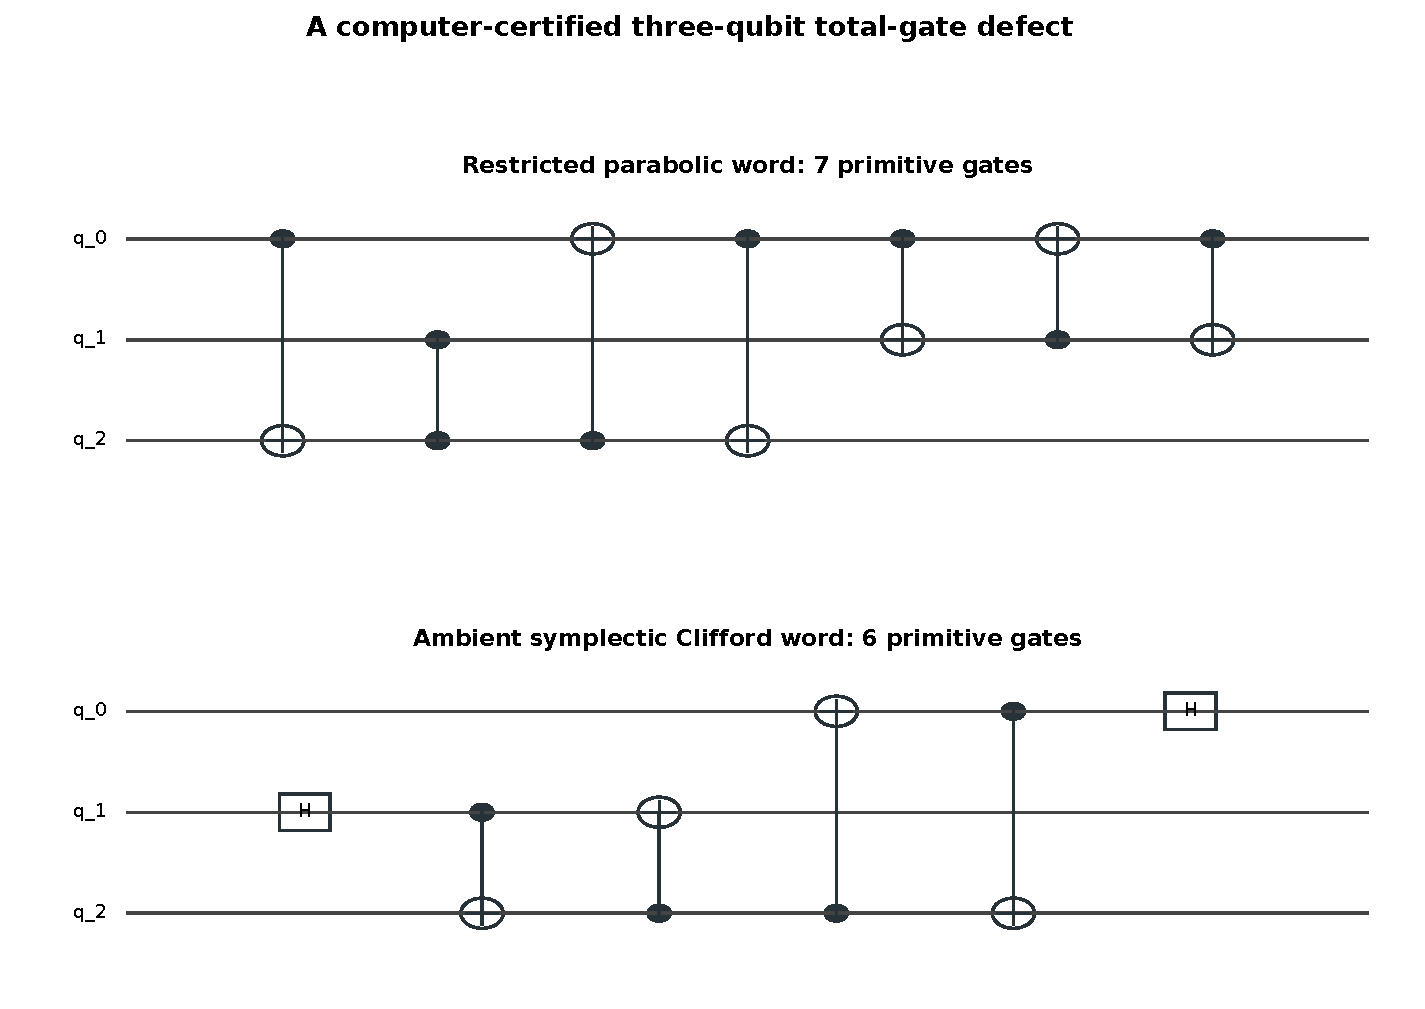
\includegraphics[width=.98\textwidth]{assets/g_clifford_three_qubit_defect.pdf}
\caption{A swap-free three-qubit parabolic target with total primitive-count defect one.}
\label{g:fig:clifford-three}
\end{figure}

The Hadamards do not form a matched pair on the same wire.  They open and close the Lagrangian excursion in different coordinates.  This is a useful warning against assuming that every catalyst has the literal form $g\cdots g^{-1}$.

\subsection{SWAP sensitivity}
Add $\SWAP_{ij}$ to both alphabets as a unit-cost primitive.  The target groups remain unchanged, but the metric changes.

\begin{computedbox}
For $n=3$ with unit-cost SWAP gates, the restricted diameter drops from eight to seven, the ambient diameter drops from twelve to eleven, and every one of the $10,752$ parabolic targets has zero total-count defect.
\end{computedbox}

The preceding twenty-four defects therefore measure a real gate-alphabet distinction, not an invariant of the subgroup inclusion alone.  In many architectures SWAP is not elementary and costs three CNOTs, while in others qubit movement or relabeling changes the accounting.  The theorem must retain the convention.

\subsection{Entangling-count defects}
Now assign cost zero to $H_i$ and $S_i$ and cost one to $\CX$ and $\CZ$.

\begin{computedbox}
The exact censuses are:
\begin{center}
\begin{tabular}{@{}rccc@{}}
\toprule
$n$&defective targets&distance pairs&maximum defect\\
\midrule
1&0&none&0\\
2&4&$(3,2)$ with multiplicity $4$&1\\
3&1,624&
$\begin{array}{c}
(3,2):24,\ (4,3):432,\ (5,4):1056,\\
(6,4):48,\ (6,5):64
\end{array}$
&2\\
\bottomrule
\end{tabular}
\end{center}
\end{computedbox}
The entangling metric has an earlier threshold and a larger exceptional set.

\subsubsection{A two-qubit witness}
A canonical target is
\[
M_2=
\begin{pmatrix}
0&1&0&0\\
1&0&0&0\\
1&1&0&1\\
1&1&1&0
\end{pmatrix}.
\]
A restricted realization is
\[
\CX_{0\to1},
S_1,
\CX_{1\to0},
\CX_{0\to1},
\]
with three entangling gates.  An ambient realization is
\[
H_1,
\CX_{1\to0},
\CX_{0\to1},
H_0,
S_1,
S_0,
\]
with two entangling gates.

\begin{figure}[ht]
\centering
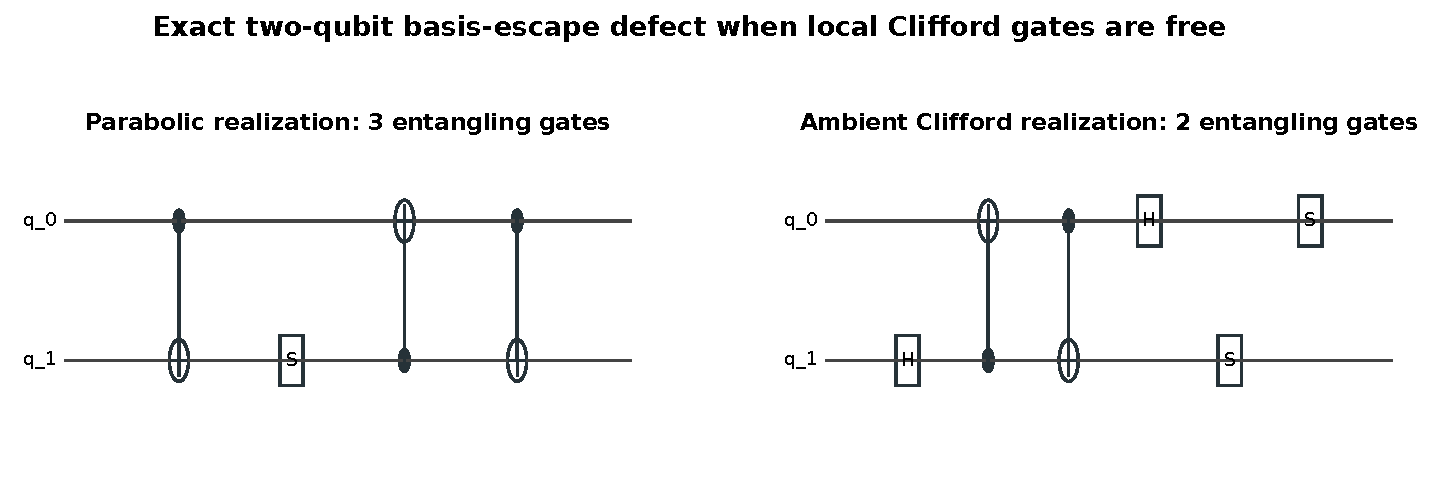
\includegraphics[width=.98\textwidth]{assets/g_clifford_two_qubit_defect.pdf}
\caption{A two-qubit entangling-count defect.  Local Clifford gates are free in this cost model.}
\label{g:fig:clifford-two}
\end{figure}

\subsection{Census summary}
\subsubsection{An analytic certificate for the four two-qubit defects}

The four exceptional matrices admit one common lower-bound proof.  Work in the declared symplectic quotient and entangling metric, with $H_i$ and $S_i$ free and SWAP excluded as a primitive.  Put
\[
J_2=\begin{pmatrix}0&1\\1&0\end{pmatrix},
\qquad D=\operatorname{diag}(d_0,d_1),
\qquad d_0,d_1\in\F_2,
\]
and define
\[
M_D=\begin{pmatrix}J_2&0\\I_2+DJ_2&J_2\end{pmatrix}.
\]

\begin{theorem}[Two-qubit orbit and exact costs]\label{g:thm:clifford-two-analytic}
Each of the four distinct matrices $M_D$ lies in $P_2$ and has restricted entangling cost three and ambient entangling cost two.  They form one orbit under left multiplication by the free restricted subgroup generated by $S_0,S_1$.
\end{theorem}
\begin{proof}
The ambient sequence
\[
H_1,\ \CX_{1\to0},\ \CX_{0\to1},\ H_0
\]
has matrix $M_0=\left(\begin{smallmatrix}J_2&0\\I_2&J_2\end{smallmatrix}\right)$.  Applying $S_0^{d_0}S_1^{d_1}$ afterwards left multiplies by $\left(\begin{smallmatrix}I_2&0\\D&I_2\end{smallmatrix}\right)$ and gives $M_D$.  These matrices are distinct because $J_2$ is invertible.  This also proves their orbit statement and the ambient upper bound two.  The displayed restricted sequence for $M_2$ above gives $M_{I_2}$ using three CNOT gates and one free $S_1$.  Free final phase gates then give every $M_D$, proving the restricted upper bound three.

For the restricted lower bound, the upper-left block of a parabolic product is the product of its upper-left blocks.  Each $S$ or CZ contributes $I_2$, while the two directed CNOTs contribute the elementary matrices
\[
L=\begin{pmatrix}1&0\\1&1\end{pmatrix},
\qquad U=\begin{pmatrix}1&1\\0&1\end{pmatrix}.
\]
Products using at most two CNOTs belong to $\{I_2,L,U,LU,UL\}$, which does not contain $J_2$.  Thus any restricted circuit for $M_D$ requires at least three charged gates.

For the ambient lower bound, reorder the coordinates as $(x_0,z_0\mid x_1,z_1)$.  A local Clifford acts by an invertible block-diagonal matrix in this order.  In $M_D$, each of the two diagonal $2\times2$ blocks is $\left(\begin{smallmatrix}0&0\\1&0\end{smallmatrix}\right)$ and has rank one.  In either directed CNOT or CZ, both diagonal blocks are $I_2$ and have rank two.  Left and right multiplication by local Cliffords preserve these diagonal-block ranks.  A circuit with one charged gate has the form $K_1 E K_2$ with $K_1,K_2$ local and $E$ a CNOT or CZ, so it cannot equal $M_D$.  A circuit with no charged gate is local and also has rank-two diagonal blocks.  The ambient cost is therefore at least two.
\end{proof}

The complete finite census finds exactly four defective targets.  Since the theorem supplies four distinct defective targets, it identifies the entire exceptional set in that census.  The exact costs and orbit description above have analytic proofs, while completeness of the finite classification retains the exhaustive-search evidence.

\begin{figure}[ht]
\centering
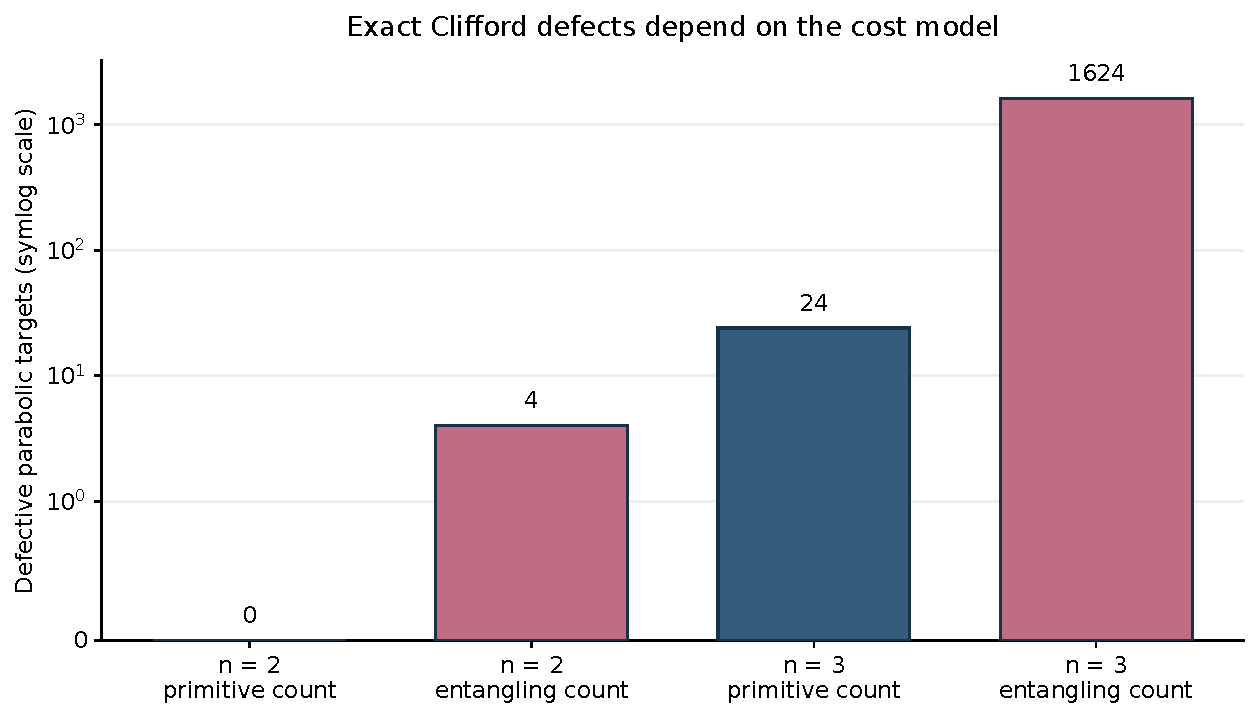
\includegraphics[width=.76\textwidth]{assets/g_clifford_census.pdf}
\caption{Exact parabolic-versus-ambient Clifford census. The vertical scale is symlogarithmic. At three qubits, adding SWAP as a unit-cost primitive removes all total-count defects.}
\label{g:fig:clifford-census}
\end{figure}

The results establish three distinct lessons.
\begin{enumerate}
\item Basis escape produces genuine Clifford defects, not only linear CNOT defects.
\item The first threshold depends on whether local gates are free.
\item Adding a SWAP primitive can eliminate a finite total-count threshold.
\end{enumerate}

\subsection{Search completeness}
The search state is the exact $2n\times2n$ binary symplectic matrix.  Every generator acts by a fixed row update.  Ordinary breadth-first search gives exact unit-cost distances.  Zero-one breadth-first search gives exact entangling costs.  Since every state of $P_n$ and $\Sp(2n,2)$ is reached, comparing the two distance maps is a complete census.

The optimized C++ verifier represents a $6\times6$ matrix by a $36$-bit integer.  It enumerates the full three-qubit group in a few seconds in the present environment.  The Python implementation is slower but independently expresses the same state model.

\subsection{Interpretation as symplectic holonomy}
The parabolic subgroup is a fiber over the Lagrangian Grassmannian.  A Hadamard moves one coordinate out of the chosen Lagrangian.  The ambient path traverses other Lagrangian frames and returns to a target stabilizing $L_Z$.

This is the symplectic analogue of the unitriangular Schreier loop.  The catalyst is a temporary exchange of $X$ and $Z$ roles.  The consumers are entangling gates that become cheaper in the changed frame.

\subsection{CSS-preserving extensions}
The parabolic model fixes one Lagrangian, but CSS circuit classes can be defined more narrowly or more broadly.  Possible restricted alphabets include:
\begin{enumerate}
\item CNOT and Pauli gates only,
\item CNOT, $S$, and diagonal controlled phases,
\item block-diagonal symplectic transformations preserving separate $X$ and $Z$ codes,
\item logical Clifford gates preserving a CSS stabilizer decomposition,
\item architecture-constrained versions of the preceding models.
\end{enumerate}
Each produces a different subgroup and metric.

\begin{skeletonbox}
A full CSS threshold paper should classify cost-preserving orbits of minimal defects, identify a symplectic-flag lower-bound invariant, and determine which defects survive when SWAP, qubit permutation, or local Cliffords are assigned alternative costs.
\end{skeletonbox}

\subsection{Depth and parallelism}
Gate-count defects do not automatically imply depth defects.  Given a gate sequence, define its dependency graph and schedule commuting or disjoint gates in parallel.  The appropriate quantities are
\[
\Delta_{\mathrm{depth}}(U),
\qquad
\Delta_{\mathrm{2q-depth}}(U),
\qquad
\Delta_{\mathrm{space-time}}(U).
\]
A basis change applied transversally to many qubits may have small depth even when its total count is large.  Conversely, a two-gate count saving can increase depth under locality constraints.

\subsection{Open Clifford problems}
\begin{question}
What are the defect orbits of the twenty-four three-qubit total-count targets under qubit permutations and parabolic conjugation?
\end{question}
\begin{question}
Does the maximum parabolic-versus-Clifford defect grow linearly, as $n\log n$, or faster under total primitive count?
\end{question}
\begin{question}
Can one prove a symbolic family with entangling-count defect greater than two, rather than relying on finite census data?
\end{question}
\begin{question}
Which finite symplectic parabolics are geodesically convex after SWAP is included as a primitive?
\end{question}
\begin{conjecturebox}
The observed three-qubit defects should admit a small collection of symplectic root motifs analogous to the three-cross, one-phase classification in the unitriangular case.  The present monograph records the exact census and witnesses but does not claim that classification.
\end{conjecturebox}

\section{Temporary nonlinearity: affine logic versus Toffoli-assisted synthesis}\label{g:ch:affine-toffoli}
\index{Toffoli gate}
\index{affine reversible circuit}
\index{temporary nonlinearity}
\index{algebraic normal form}


\subsection{The question}
Let
\[
\operatorname{AGL}(n,2)
=
\{x\mapsto Ax+b:A\in\GL(n,2),\ b\in\F_2^n\}
\]
be the affine reversible group.  It is generated by NOT and CNOT gates.  The ambient gate set adds Toffoli.  On three bits it generates the full reversible group.  On $n\ge4$ bits with no ancillas, each NOT, CNOT, or Toffoli gate is an even permutation, so this alphabet does not generate the full symmetric group.

The catalytic question is:
\begin{quote}
Can a circuit temporarily create nonlinear Boolean terms with Toffoli gates, reuse them, cancel them completely, and implement a final affine permutation with fewer gates than every affine circuit?
\end{quote}
This is the nonlinear analogue of dirty linear memory.

\subsection{Algebraic normal form}
Every Boolean coordinate function has a unique algebraic normal form
\[
f_i(x)
=
\bigoplus_{S\subseteq[n]}a_{i,S}\prod_{j\in S}x_j.
\]
Affine maps have degree at most one.  A Toffoli gate targeting $t$ with controls $a,b$ performs
\[
x_t\longmapsto x_t+x_ax_b,
\]
which can raise the degree of later coordinates.  The final affine target requires every higher-degree coefficient to cancel.

A candidate lower-bound invariant must do more than track maximum degree.  One Toffoli creates degree two and a second can remove it.  Useful refinements include:
\begin{itemize}
\item the dimension of the quadratic monomial span,
\item directional derivatives $D_u f(x)=f(x+u)+f(x)$,
\item the rank of the bilinear polarization,
\item the number of outputs consuming a nonlinear workspace term,
\item restoration obligations for every nonlinear carrier.
\end{itemize}

\subsection{Exact three-bit census}
On three bits,
\[
|\operatorname{AGL}(3,2)|
=2^3|\GL(3,2)|
=1344,
\]
while the group generated by NOT, CNOT, and Toffoli is the full permutation group
\[
S_8,
\qquad |S_8|=40320.
\]
Both spaces can be enumerated exactly.

\begin{computedbox}
For three bits, every affine target has the same minimum cost in the affine gate set and in the Toffoli-assisted gate set under each of the following metrics:
\begin{enumerate}
\item total primitive gate count, where NOT, CNOT, and Toffoli cost one,
\item entangling count, where NOT is free and CNOT and Toffoli cost one.
\end{enumerate}
There are no defective affine targets among all $1344$ targets.
\end{computedbox}

The restricted total-count diameter is seven and the ambient diameter on $S_8$ is eight.  Under entangling count, both relevant diameters are six.  Equality on affine targets is stronger than a diameter comparison because every target is checked individually.

\begin{figure}[ht]
\centering
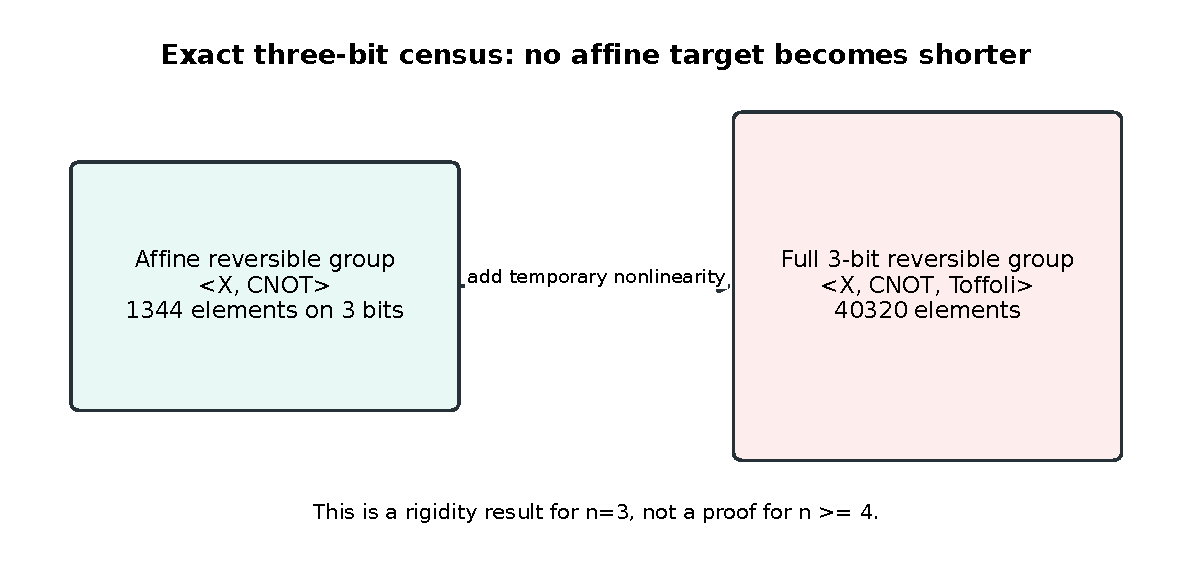
\includegraphics[width=.84\textwidth]{assets/g_affine_toffoli_census.pdf}
\caption{The complete three-bit affine-versus-Toffoli census is rigid.}
\label{g:fig:affine-toffoli-census}
\end{figure}

\subsection{Interpretation of the negative result}
The census does not show that temporary nonlinearity is useless in general.  It shows that three bits do not provide enough state space for a nonlinear carrier to repay its creation and cancellation cost under the stated alphabets.

The negative result is valuable for three reasons.
\begin{enumerate}
\item It gives a certified lower threshold: any total- or entangling-count defect requires at least four bits.
\item It prevents a forced analogy with the six-wire linear catalyst.
\item It supplies a complete regression test for future synthesis code.
\end{enumerate}

\subsection{A formal nonlinear catalyst}
A clean one-workspace template is
\[
T\;h_m\cdots h_1\;T^{-1},
\]
where $T$ is Toffoli and the middle gates use the quadratic term created in the workspace.  Since Toffoli is self-inverse, the displayed circuit uses two nonlinear gates.

\begin{figure}[ht]
\centering
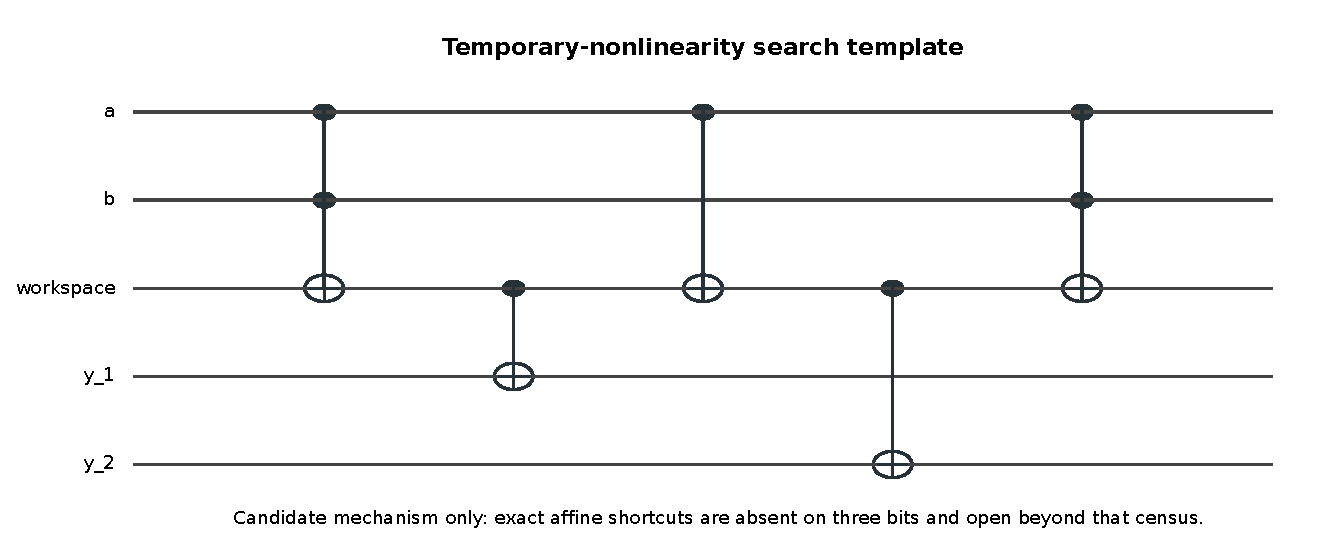
\includegraphics[width=.96\textwidth]{assets/g_temporary_nonlinearity_skeleton.pdf}
\caption{A temporary-nonlinearity template.  It is a search skeleton, not a proved shortcut.}
\label{g:fig:nonlinear-skeleton}
\end{figure}

The key difficulty is that a final affine map cannot retain any product term.  Every output that consumed the nonlinear carrier must be repaired, or the nonlinear contributions must cancel collectively.

\subsection{Conjugation formulas}
Let $T_{ab\to t}$ denote Toffoli.  Conjugating an affine gate by $T$ can produce nonlinear permutations.  For example, if $X_t$ flips the target,
\[
T_{ab\to t}X_tT_{ab\to t}=X_t,
\]
so no gain occurs.  If a CNOT changes a control or exports the target, the conjugated map can contain several quadratic terms.  The exact formula is easiest in algebraic normal form: substitute the Toffoli-updated coordinate into the affine map, then apply the inverse substitution.

A systematic search should classify pairs $(T,h)$ for which
\[
ThT^{-1}\in\operatorname{AGL}(n,2).
\]
For one Toffoli and an affine middle word, this is a normalizer-intersection problem.  A useful next bounded test is to examine simple two-Toffoli sandwiches with an affine middle word of restricted length at most five.  The present archive contains no reproducible implementation or receipt for this four-bit test, so no negative result from it is claimed here.

\subsection{Potential lower-bound invariants}
\subsubsection{Quadratic support debt}
Let $Q(f)$ be the span of quadratic monomials appearing across the coordinate functions.  A Toffoli changes $Q(f)$ by at most a controlled rank-one contribution before subsequent substitutions.  If several outputs consume the same quadratic term, a dynamic debt invariant may charge its creation, distribution, and cancellation.

\subsubsection{Derivative rank}
For an affine map, every derivative $D_u f$ is constant.  During a nonlinear excursion, the derivative map
\[
u\mapsto D_u f(x)
\]
can depend on $x$.  One can track the dimension of the nonconstant derivative space and require it to return to zero.

\subsubsection{Higher-order Möbius coefficients}
The ANF coefficients are the Möbius transform of the truth table.  Projectors onto degree layers give an exact packet decomposition
\[
f=f^{(0)}+f^{(1)}+f^{(2)}+\cdots.
\]
A restricted affine circuit remains in degrees zero and one.  The ambient circuit can populate higher packets temporarily.  A successful lower bound must charge the useful flow through those packets, not merely their instantaneous dimension.

\subsection{Four-bit search architecture}
The full permutation group on four-bit states has size $16!$.  The declared no-ancilla gate alphabet lies in its alternating subgroup: NOT, CNOT, and Toffoli are respectively products of eight, four, and two disjoint transpositions.  Even this reduced ambient search is large enough to require a more structured approach.  Several exact approaches remain available.
\begin{enumerate}
\item Meet in the middle for a fixed candidate target and length.
\item SAT or SMT encoding of a length-$L$ circuit with affine endpoint constraints.
\item Bidirectional search restricted to states within a bounded nonlinear-degree or Toffoli-count budget.
\item Enumeration of two- or four-Toffoli normal forms modulo affine conjugation.
\item Mixed-integer or algebraic solving of ANF coefficient equations.
\end{enumerate}

\begin{protocol}[First four-bit threshold search]
\begin{enumerate}
\item Compute exact affine distances for all $322{,}560$ affine targets.
\item Enumerate ambient words with two Toffoli gates modulo affine gates on the left and right.
\item Retain words whose endpoint is affine.
\item Compare with the exact affine distance.
\item If no defect appears, increase the Toffoli budget and produce an unsatisfiability certificate for every shorter length.
\end{enumerate}
\end{protocol}
This protocol is a research plan.  The packaged executable census stops at three bits, and neither the four-bit normal-form search nor its lower-bound certificates is supplied.

\subsection{Resource variants}
Temporary nonlinearity may be useful under one metric and useless under another.  Natural costs include:
\[
\begin{gathered}
\text{Toffoli count},\quad \text{CNOT count},\quad
T\text{-count after decomposition},\quad T\text{-depth},\\
\text{ancilla count},\quad \text{total depth}.
\end{gathered}
\]
A Toffoli-assisted affine shortcut in total Boolean gates might disappear after fault-tolerant decomposition.  Conversely, a circuit with more Boolean primitives can reduce $T$-depth.

\subsection{Related nonlinear gate families}
The same program applies to:
\begin{itemize}
\item CCZ-assisted diagonal Boolean phase maps,
\item relative-phase Toffoli gates,
\item multi-controlled $X$ and $Z$ gates,
\item Reed--Muller degree hierarchies,
\item reversible arithmetic over $\Z_d$,
\item polynomial automorphisms over finite rings.
\end{itemize}

\begin{conjecturebox}
There exists an affine target on finitely many bits whose total or fault-tolerant resource cost is reduced by a restored nonlinear excursion.  The exact three-bit census rules out the smallest possible instance but supplies no evidence for a particular larger threshold.
\end{conjecturebox}

\subsection{Reproducible code}
The implementation represents every reversible map as an exact permutation of $2^n$ basis states.  Breadth-first search enumerates both the affine group and the full three-bit reversible group.

\begin{lstlisting}[style=pythonstyle,caption={Exact three-bit affine-versus-Toffoli census.}]
from catalytic_gate_atlas import exact_affine_toffoli_census

print(exact_affine_toffoli_census(3, entangling_cost=False))
print(exact_affine_toffoli_census(3, entangling_cost=True))
\end{lstlisting}
The expected defect count is zero in both outputs.

\section{Phase-polynomial and Clifford+\texorpdfstring{$T$}{T} catalysis}\label{g:ch:phase-cliffordt}
\index{Clifford+T circuit}
\index{phase polynomial}
\index{T-count}
\index{T-depth}
\index{Pareto defect}


\subsection{Why the phase setting is different}
Fault-tolerant quantum compilation rarely assigns equal cost to every gate.  Clifford operations are often treated as inexpensive relative to non-Clifford gates, while connectivity and parity computation can dominate the remaining cost.  Consequently there is no single Clifford+$T$ defect.  One must specify at least
\[
\mathbf c(U)=
\bigl(
T\text{-count},
T\text{-depth},
\text{two-qubit count},
\text{two-qubit depth},
\text{ancillas}
\bigr).
\]
A catalytic excursion may improve one component and worsen another.  The natural comparison is therefore Pareto-valued rather than scalar unless a hardware-specific weight vector is fixed.

Let $\omega=e^{i\pi/4}$.  A phase-polynomial circuit on $n$ qubits has the form \cite{g:AmyMosca2019,g:Selinger2013}
\begin{equation}\label{g:eq:phase-poly-normal}
U\ket{x}=\omega^{P(x)}\ket{Ax+b},
\end{equation}
where $A\in\GL(n,2)$, $b\in\F_2^n$, and $P:\F_2^n\to\Z_8$ is represented as a sum of binary linear forms with coefficients in $\Z_8$.  The diagonal case has $A=I$ and $b=0$.

The restricted model may be chosen in several ways:
\begin{enumerate}
\item diagonal phase gadgets only;
\item CNOT-dihedral circuits generated by $X$, CNOT, and $T$;
\item parity networks in which every intermediate transformation remains affine on computational basis labels;
\item a prescribed family of commuting Pauli rotations.
\end{enumerate}
The ambient model may add Hadamards, arbitrary Clifford conjugations, measurements, or ancillas.  These choices define different problems.

\subsection{Pauli-rotation language}
For a Pauli operator $P$ and angle $\theta$, write
\[
R_P(\theta)=e^{-i\theta P/2}.
\]
Every Clifford $C$ satisfies
\begin{equation}\label{g:eq:pauli-conjugation}
C R_P(\theta) C^\dagger=R_{CPC^\dagger}(\theta).
\end{equation}
Thus a short ambient basis change can rotate a large family of phase gadgets into a different commuting or nearly commuting family, apply them there, and rotate back.

\begin{provedbox}
Equation \eqref{g:eq:pauli-conjugation} is an exact catalytic transport identity.  It does not by itself prove a gate-count defect.  A defect additionally requires a lower bound showing that the transported family is more expensive in the restricted representation than the opening and closing Clifford layers plus the transported implementation.
\end{provedbox}

The simplest symbolic sandwich is
\[
C\left(\prod_{j=1}^m R_{P_j}(\theta_j)\right)C^\dagger
=
\prod_{j=1}^m R_{CP_jC^\dagger}(\theta_j).
\]
If the $P_j$ commute, their conjugates commute.  A catalyst can therefore change the geometry of the support without changing the algebra of the angles.

\subsection{Phase polynomials and parity carriers}
A CNOT network computes linear parities
\[
\lambda(x)=a\cdot x\in\F_2.
\]
Applying $T^k$ to a wire carrying $\lambda(x)$ contributes
\[
\omega^{k\lambda(x)}
\]
to the phase polynomial.  A parity network must create each required parity, expose it to a phase gate, and restore the linear map required at the endpoint.

This makes phase-polynomial synthesis a close relative of the snapshot families in the linear core.  A parity row may evolve through
\[
\lambda_0,\lambda_1,\ldots,\lambda_m,
\]
with selected states consumed by phase gates.  The difference is that consumption need not copy the parity to another row; it can deposit phase while leaving the carrier unchanged.

\begin{skeletonbox}
A candidate phase catalyst consists of:
\begin{enumerate}
\item a Clifford $C$ that opens a non-diagonal frame;
\item an evolving Pauli or parity carrier in that frame;
\item several phase rotations consuming intermediate carrier states;
\item $C^\dagger$ restoring the original diagonal or CNOT-dihedral model;
\item a certificate that no restricted parity network attains the same resource vector.
\end{enumerate}
\end{skeletonbox}

\begin{figure}[ht]
\centering
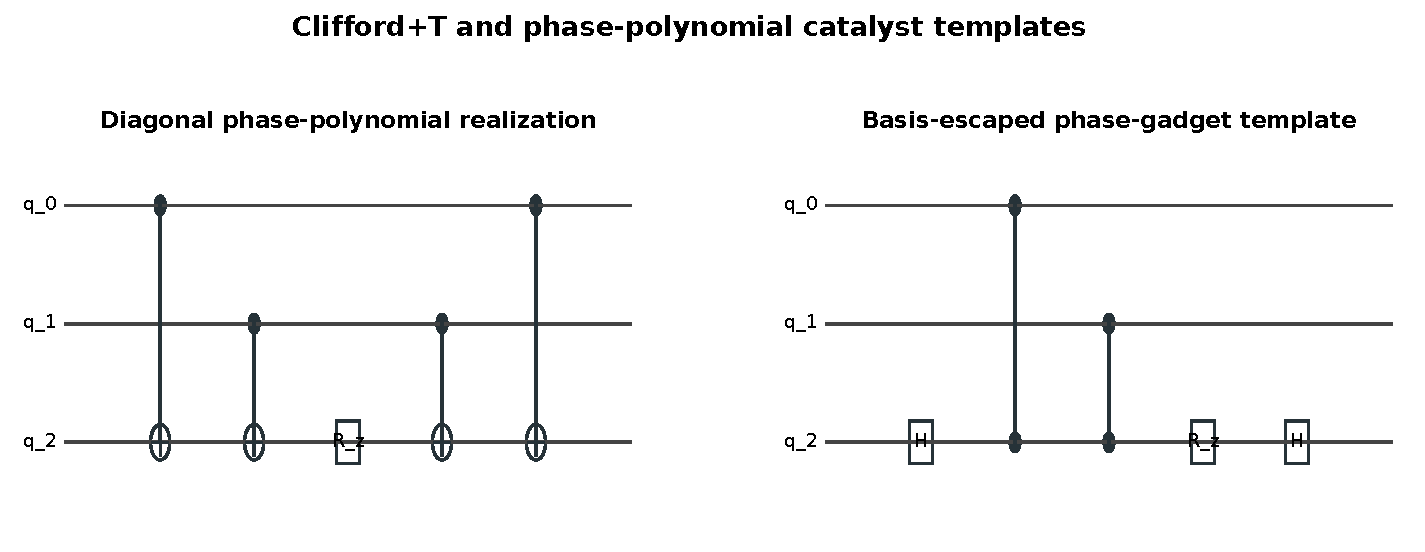
\includegraphics[width=.94\textwidth]{assets/g_phase_polynomial_skeleton.pdf}
\caption{Symbolic Clifford+$T$ catalyst: a basis excursion transports a family of phase obligations and is removed at the endpoint.}
\label{g:fig:phase-polynomial-skeleton}
\end{figure}

\subsection{\texorpdfstring{$T$}{T}-count as a coding problem}
For diagonal Clifford+$T$ synthesis without ancillas, equivalent phase-polynomial descriptions can differ by identities whose coefficients vanish modulo eight on Boolean inputs.  Minimizing the number of odd coefficients is naturally expressed as a coset-decoding problem in a punctured Reed--Muller-type code.

Let $a\in\Z_8^{2^n-1}$ index nonzero linear forms and let $\operatorname{odd}(a)$ denote the binary vector recording which coefficients are odd.  An abstract restricted $T$-count is
\[
\ell_T(P)=
\min_{a:\,P_a=P}
\operatorname{wt}(\operatorname{odd}(a)).
\]
An ambient Clifford excursion changes not only the coefficient vector but also the Pauli frame in which the rotations are represented.  A lower bound that survives ambient Clifford conjugation must therefore be invariant under the relevant symplectic action or must explicitly charge the frame change.

\subsection{\texorpdfstring{$T$}{T}-depth and commuting layers}
Two phase gadgets may share a $T$ layer when a suitable Clifford network maps their parities to distinct wires or when ancilla resources permit parallel extraction.  Define the conflict graph $\Gamma_P$ whose vertices are odd phase terms and whose edges encode inability to realize two terms in one layer under the chosen ancilla and connectivity rules.  Then
\[
T\text{-depth}(P)\ge\chi(\Gamma_P)
\]
for any conflict graph whose edge relation is sound.  Catalysis can alter $\Gamma_P$ by changing the Pauli frame.  The right question is not merely whether $C$ preserves the number of terms, but whether it reduces the chromatic or scheduling obstruction enough to repay its own depth.

\subsection{A vector-valued defect}
For a target $U$ in a restricted phase model, define
\[
\mathcal C_{\mathrm{res}}(U)
=
\{\mathbf c(\mathcal W):\mathcal W\text{ is a restricted circuit for }U\}
\]
and similarly $\mathcal C_{\mathrm{amb}}(U)$.  Their Pareto frontiers are denoted $\operatorname{Pareto}_{\mathrm{res}}(U)$ and $\operatorname{Pareto}_{\mathrm{amb}}(U)$.

\begin{definition}[Pareto catalytic defect]
A target has a Pareto catalytic defect when the ambient Pareto frontier contains a point strictly dominating every restricted cost vector in at least one declared region of resource space.
\end{definition}

Scalarization by positive weights $w$ gives
\[
\Delta_w(U)=
\min_{c\in\mathcal C_{\mathrm{res}}(U)}w\cdot c
-
\min_{c\in\mathcal C_{\mathrm{amb}}(U)}w\cdot c.
\]
Different $w$ can change the magnitude of the defect and whether it is zero or positive.  It remains nonnegative because every restricted realization is also an ambient realization with the same resource vector.

\subsection{Exact finite-search model}
A finite exact atlas can be built \cite{g:KliuchnikovEtAl2013,g:AmyEtAl2013} for small $n$ by representing Clifford+$T$ operators in one of three ways.
\begin{enumerate}
\item Exact matrices over the cyclotomic ring $\Z[1/\sqrt2,i]$ modulo global phase.
\item Normal forms combining a binary symplectic Clifford with a phase-polynomial record.
\item Quotients by left and right Clifford actions when only $T$-count is charged.
\end{enumerate}
The third model can be dramatically smaller but requires care: quotienting is sound only when the free Clifford actions in the cost model agree with the quotient relation.

\begin{protocol}[Small-width Clifford+$T$ threshold atlas]
\begin{enumerate}
\item Fix exact versus approximate synthesis, ancilla rules, and the resource vector.
\item Enumerate the restricted target subgroup or a complete set of normal forms.
\item Compute restricted Pareto frontiers by multiobjective shortest path.
\item Enumerate ambient states or use meet in the middle for candidate targets.
\item Store an optimal witness and a lower-bound certificate for every defect.
\item Classify defects under qubit permutation and free Clifford equivalence.
\end{enumerate}
\end{protocol}

\subsection{Lower-bound candidates}
\subsubsection{Odd-support rank}
The span of odd phase terms is invariant under some restricted rewrites but transforms covariantly under linear changes of variables.  Its dimension gives a coarse obstruction.

\subsubsection{Pauli support geometry}
Represent a commuting Pauli family by an isotropic subspace of $\F_2^{2n}$.  Restricted diagonal circuits remain in the $Z$ Lagrangian.  Ambient Clifford circuits move through the symplectic Grassmannian.  Distance from the $Z$ Lagrangian, together with the number of deposited rotations, is the phase analogue of microscopic flag escape.

\subsubsection{Moment and derivative packets}
For a phase function $P$, finite differences
\[
D_uP(x)=P(x+u)-P(x)\pmod8
\]
separate affine, quadratic, and higher interactions.  A hierarchy of derivative tensors can record temporary flow into nonlinear phase packets.

\subsubsection{Architecture-aware parity rank}
On a coupling graph, each parity has a Steiner cost.  A catalyst can be profitable by making several required parities share a Steiner tree.  A sound lower bound may combine cut rank with edge congestion and restoration debt.

\subsection{Tensor and repeated-module questions}
For targets $U$ and $V$, independent synthesis gives
\[
\ell_T(U\otimes V)
\le
\ell_T(U)+\ell_T(V)
\]
when the systems are disjoint and local Clifford cost is ignored.  Joint synthesis may be better because phase identities can couple terms across modules.  This motivates a stable regularization
\[
\tau_T(U)=
\liminf_{r\to\infty}
\frac{\ell_T(U^{\otimes r})}{r}.
\]
A one-copy rigid phase target could still display tensor activation.

\begin{conjecturebox}
There are diagonal or CNOT-dihedral targets whose Pareto frontier is strictly improved by a restored non-diagonal Clifford excursion.  The smallest qubit threshold and the resource component in which the first defect appears are open in this monograph.
\end{conjecturebox}

\subsection{What would count as a theorem}
A publishable first result in this direction should contain all of the following:
\begin{enumerate}
\item an exact target family and gate alphabets;
\item explicit ambient circuits;
\item a restricted lower bound for the same declared cost;
\item exact treatment of global phase and ancillas;
\item classification below the first threshold or a proof of minimality;
\item reproducible symbolic code.
\end{enumerate}
Merely rewriting a phase gadget with Hadamards is not sufficient.  The decisive content is the optimality comparison.

\section{Gaussian, matchgate, and fermionic catalytic models}\label{g:ch:gaussian}
\index{Gaussian circuit}
\index{matchgate}
\index{Bogoliubov transformation}
\index{fermionic Gaussian circuit}
\index{symplectic embedding}


\subsection{Two Gaussian settings}
Quantum Gaussianity occurs \cite{g:WeedbrookEtAl2012} in two closely related but algebraically different settings.

For $n$ bosonic modes, a Gaussian unitary acts on quadratures
\[
\mathbf r=(q_1,\ldots,q_n,p_1,\ldots,p_n)^T
\]
by an affine symplectic transformation
\[
\mathbf r\longmapsto S\mathbf r+d,
\qquad
S\in\Sp(2n,\R).
\]
For $n$ fermionic modes, a fermionic Gaussian unitary acts on $2n$ Majorana operators by
\[
\gamma\longmapsto O\gamma,
\qquad O\in SO(2n).
\]
Nearest-neighbor matchgates give a circuit presentation of a fermionic Gaussian subgroup on qubits.

In both cases one can choose a restricted subgroup preserving a flag, mode ordering, particle number, or bipartition, and compare it with a larger Gaussian or non-Gaussian gate set.

\subsection{An inherited symplectic shear theorem}
Every invertible linear transformation $A\in\GL(n,R)$ has a canonical symplectic embedding
\begin{equation}\label{g:eq:symplectic-embedding}
\iota(A)=
\begin{pmatrix}
A&0\\
0&A^{-T}
\end{pmatrix}.
\end{equation}
Indeed, with
\[
J=
\begin{pmatrix}0&I\\-I&0\end{pmatrix},
\]
one checks
\[
\iota(A)^T J\iota(A)=J.
\]
Thus every row-transvection identity in the established linear theory induces an exact identity between symplectic shear circuits.

\begin{provedbox}
Under a Gaussian gate alphabet in which each embedded elementary transvection $\iota(I+aE_{ij})$ is one primitive and direction is the only restriction, the universal six-row catalytic atom embeds into a twelve-quadrature Gaussian atom with restricted length seven and ambient length six.
\end{provedbox}

This is a formal inheritance statement for the declared shear alphabet.  It does not assert optimality after arbitrary beam splitters, squeezers, Fourier transforms, or local Gaussian gates are admitted at unit cost.

\begin{figure}[ht]
\centering
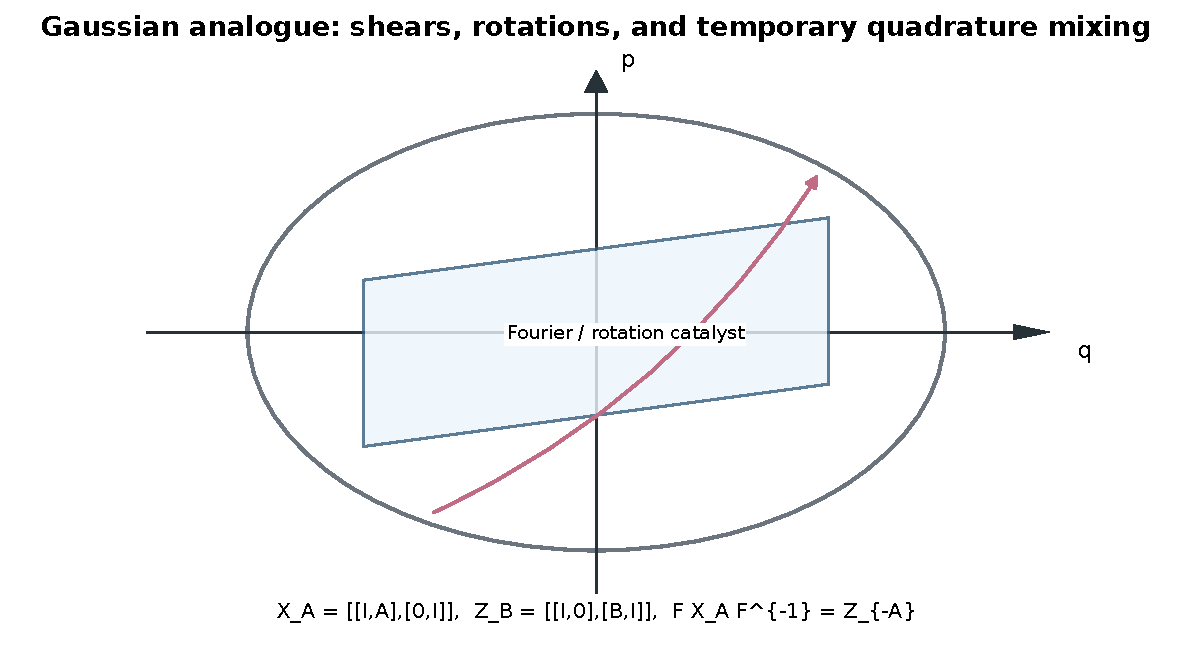
\includegraphics[width=.94\textwidth]{assets/g_gaussian_shear_catalysis.pdf}
\caption{The row-transvection atom embedded as a Gaussian symplectic shear circuit.}
\label{g:fig:gaussian-shear}
\end{figure}

\subsection{Bosonic gate hierarchies}
Natural nested models include
\[
\text{triangular shears}
\subset
\text{all Gaussian unitaries}
\subset
\text{Gaussian plus a non-Gaussian primitive}
\subset
U(\mathcal H).
\]
Typical primitive resources are:
\begin{itemize}
\item SUM or controlled displacement gates,
\item beam splitters,
\item single-mode and two-mode squeezers,
\item Fourier transforms,
\item cubic phase gates,
\item photon counting or non-Gaussian state injection.
\end{itemize}
Each inclusion supports a different defect.  A target Gaussian transformation might be shortened by leaving a triangular decomposition but remaining Gaussian.  A more radical question asks whether temporary non-Gaussianity can shorten a final Gaussian target.

\subsection{Bloch--Messiah versus catalytic synthesis}
A bosonic Gaussian unitary admits a Bloch--Messiah decomposition
\[
S=K_1 D K_2,
\]
where $K_1,K_2$ are passive symplectic transformations and $D$ is a diagonal squeezing layer.  This normal form optimizes conceptual structure, not necessarily a weighted gate count on a specific architecture.

Catalytic synthesis asks whether a short excursion into a basis where many shear or squeezing obligations align can reduce total cost.  The opening and closing passive layers play the role of the catalyst.

\begin{skeletonbox}
A Gaussian catalytic theorem requires:
\begin{enumerate}
\item a declared primitive library and cost vector;
\item a target subgroup, such as triangular, number conserving, or local;
\item an explicit sandwich $KHK^{-1}$ returning to the target subgroup;
\item a lower bound based on symplectic rank, singular values, graph cuts, or mode support;
\item treatment of approximation error when continuous parameters are synthesized numerically.
\end{enumerate}
\end{skeletonbox}

\subsection{Fermionic Gaussian and matchgate circuits}
Let $c_j,c_j^\dagger$ be fermionic creation and annihilation operators.  Quadratic Hamiltonians generate Gaussian unitaries, and their action is determined by an orthogonal transformation on Majoranas.  Number-conserving Gaussian operations correspond to a unitary action on modes, while general Gaussian operations allow particle-hole mixing.

This yields the hierarchy
\[
\begin{gathered}
U(n)\text{ mode transformations}
\subset SO(2n)\text{ fermionic Gaussian transformations}\\
\subset \text{parity-preserving unitaries}.
\end{gathered}
\]
A temporary Bogoliubov transformation can violate number conservation while preserving parity.  The target may nevertheless return to the number-conserving subgroup.

\begin{definition}[Bogoliubov catalytic defect]
For a number-conserving Gaussian target $U$, compare the minimum cost using number-conserving primitives with the minimum cost using general Gaussian primitives, requiring the endpoint to conserve number exactly.
\end{definition}

\subsection{Matchgates and geometry}
Nearest-neighbor matchgate circuits \cite{s:Valiant2002,s:JozsaMiyake2008} have strong classical simulation properties.  Their geometry changes when SWAP, fermionic SWAP, long-range connectivity, or a single non-matchgate resource is added.  Candidate restricted/ambient pairs include:
\begin{enumerate}
\item nearest-neighbor matchgates versus all-to-all matchgates;
\item number-conserving matchgates versus general matchgates;
\item matchgates versus parity-preserving two-qubit gates;
\item Gaussian circuits versus Gaussian circuits with one reusable non-Gaussian ancilla.
\end{enumerate}

A compiler application is immediate: a temporary mode permutation or particle-hole rotation may allow a batch of otherwise expensive interactions to share one routing or basis-change layer.

\subsection{Covariance-matrix lower bounds}
For a Gaussian state, the covariance matrix $\Gamma$ transforms as
\[
\Gamma\longmapsto S\Gamma S^T
\]
in the bosonic case and
\[
\Gamma\longmapsto O\Gamma O^T
\]
in the fermionic case.  Possible restricted lower bounds include:
\begin{itemize}
\item rank change of off-diagonal covariance blocks,
\item symplectic singular-value obligations,
\item growth of mode support,
\item graph bandwidth and cut rank,
\item number of nontrivial canonical angles between invariant subspaces.
\end{itemize}
One elementary gate changes only a controlled portion of these data.  A useful invariant must also charge preparation of a carrier that makes progress on many cuts simultaneously.

\subsection{Temporary non-Gaussianity}
Suppose a non-Gaussian primitive $g$ is introduced and later removed:
\[
U=g h_m\cdots h_1 g^{-1},
\qquad U\in G_{\mathrm{Gauss}}.
\]
If $g h_i g^{-1}$ generates several useful Gaussian effects, the excursion may be catalytic.  However, many standard non-Gaussianity monotones vanish only on states rather than unitaries, and cancellation at the endpoint complicates direct lower bounds.

Candidate monotones and certificates include:
\begin{itemize}
\item degree in the Weyl characteristic function,
\item Wigner negativity generated during the path,
\item operator Schmidt rank across mode cuts,
\item polynomial degree of Heisenberg-evolved quadratures,
\item stabilizer rank for encoded finite-dimensional subspaces.
\end{itemize}

\subsection{Exact and numerical search}
Finite exact enumeration is available for binary symplectic or orthogonal quotients, but continuous Gaussian groups require a different strategy.
\begin{enumerate}
\item Fix a symbolic gate skeleton and solve polynomial equations for parameters.
\item Use interval arithmetic to certify nonexistence below a length.
\item Exploit canonical decompositions to quotient local or passive layers.
\item For discrete-angle Gaussian libraries, use exact algebraic-number arithmetic.
\item Store both an upper-bound circuit and a dual or algebraic certificate.
\end{enumerate}

\subsection{Architecture and routing}
On a line or grid, Gaussian and matchgate circuits may be dominated by routing.  Let $G_{\mathrm{conn}}$ be the hardware graph.  A mode permutation $\pi$ can be treated as a catalyst if it is opened, many interactions are executed in the reordered frame, and $\pi^{-1}$ restores the logical labeling.  The benefit is
\[
\text{routing saved across consumers}
-
2\,\text{cost}(\pi).
\]
This is the same amortization law as the linear snapshot family, now applied to mode geometry.

\begin{conjecturebox}
There exist number-conserving or nearest-neighbor Gaussian targets whose minimum weighted cost is reduced by a restored Bogoliubov, mode-permutation, or non-Gaussian excursion.  The first exact threshold depends on the primitive library and is not determined here.
\end{conjecturebox}

\subsection{Research deliverables}
A complete Gaussian extension should produce:
\begin{enumerate}
\item a finite or semialgebraic model with exact endpoint equality;
\item at least one nontrivial lower-bound invariant;
\item a minimal catalytic atom;
\item a weighted hardware interpretation;
\item a tensor or repeated-mode amplification theorem;
\item code using exact arithmetic or certified intervals.
\end{enumerate}

\section{Symmetry, ancillas, measurement, and architecture}\label{g:ch:symmetry-measurement}
\index{symmetry-preserving circuit}
\index{ancilla}
\index{measurement and feedforward}
\index{architecture constraint}
\index{resource theory}


\subsection{Beyond subgroup word metrics}
Some of the most important quantum resource enlargements are not inclusions of groups.  Measurement introduces branches, reset is irreversible, and ancillas enlarge the Hilbert space.  The appropriate abstraction is a nested pair of realization categories
\[
\mathcal C_{\mathrm{res}}
\subseteq
\mathcal C_{\mathrm{amb}},
\]
with a cost assigned to generating morphisms.

For a target channel $\Phi$ in the restricted category, define
\[
c_{\mathrm{res}}(\Phi)
=
\inf\{\cost(W):W\text{ realizes }\Phi\text{ in }\mathcal C_{\mathrm{res}}\}
\]
and similarly $c_{\mathrm{amb}}(\Phi)$.  The value $+\infty$ is allowed.  A finite positive difference is a metric defect; an infinite difference is an existence defect.

\subsection{Symmetry-preserving circuits}
Let $Q$ be a conserved charge and let
\[
H_Q=\{U:[U,Q]=0\}.
\]
Restricted circuits use gates commuting with $Q$.  Ambient circuits may temporarily leave $H_Q$ but must return to a charge-preserving endpoint.

Examples include:
\begin{itemize}
\item particle-number conservation,
\item parity conservation,
\item total spin or magnetization,
\item lattice gauge constraints,
\item stabilizer or CSS sector preservation,
\item block-diagonal representation sectors.
\end{itemize}

The Hilbert space decomposes as
\[
\mathcal H=\bigoplus_q\mathcal H_q.
\]
A restricted circuit is block diagonal.  An ambient catalyst may couple sectors, use the enlarged route, and decouple them at the endpoint.

\begin{skeletonbox}
A symmetry-breaking catalyst has three obligations:
\begin{enumerate}
\item quantify how far the path leaves the symmetry algebra;
\item prove exact return, not merely return on a chosen input state;
\item compare the cost with every symmetry-preserving realization of the full target operator.
\end{enumerate}
\end{skeletonbox}

\subsection{Sector-flow invariants}
Let $P_q$ be the projector onto sector $q$.  For an intermediate unitary $U_t$, define transfer blocks
\[
T_{q,r}(t)=P_q U_t P_r.
\]
A restricted path has $T_{q,r}=0$ for $q\ne r$.  Ambient paths may populate off-diagonal blocks.  Possible excursion measures include
\[
\sum_{q\ne r}\rank T_{q,r},
\qquad
\max_{q\ne r}\|T_{q,r}\|,
\qquad
\text{bandwidth in }|q-r|.
\]
These are analogues of strict-upper rank and bandwidth in the unitriangular theory.

\subsection{Clean and dirty ancillas}
A clean ancilla starts in a specified state, usually $\ket0$, and must be returned to that state.  A dirty ancilla starts in an unknown state and must be restored for every input.

Let $U$ act on the data register.  A clean-ancilla realization is a unitary $W$ satisfying
\[
W(\ket\psi\otimes\ket0)
=(U\ket\psi)\otimes\ket0
\quad\text{for every }\ket\psi.
\]
A dirty-ancilla realization requires
\[
W(\ket\psi\otimes\ket\phi)
=(U\ket\psi)\otimes\ket\phi
\quad\text{for every }\ket\psi,\ket\phi.
\]
The second condition is strictly stronger.

Ancillas define a family of defects
\[
\Delta_{a,\mathrm{clean}}(U),
\qquad
\Delta_{a,\mathrm{dirty}}(U),
\]
where $a$ is the number of ancillary qubits or modes.  Stable ancilla capacity asks whether a fixed number of reusable ancillas can yield an unbounded saving as the data size grows.

\subsection{Measurement and feedforward}
A measurement-assisted realization is described by an instrument with classical outcomes $m$, conditional channels $\Phi_m$, and feedforward operations.  Exact deterministic implementation of a unitary target requires every branch, after correction, to induce the same channel.

The cost vector may include
\[
(
T\text{-count},
\text{two-qubit count},
\text{measurement rounds},
\text{classical latency},
\text{ancilla qubits}
).
\]
A measurement can create an existence defect by realizing a channel unavailable unitarily under the same locality or depth constraints, or a metric defect by reducing one resource while increasing another.

\begin{definition}[Branch-catalytic realization]
A measurement-assisted circuit is branch catalytic when the intermediate classical or quantum branch information is absent from the final data channel and all declared work systems are reset or discarded according to the model.
\end{definition}

\subsection{Teleportation as a canonical ambient excursion}
Gate teleportation replaces direct implementation by:
\[
\text{prepare resource state}
\to
\text{entangle and measure}
\to
\text{classical correction}.
\]
The ambient category contains resources not present in the target channel: entanglement, measurement outcomes, and feedforward.  The endpoint can nevertheless be a deterministic unitary.

This is an archetypal realization defect, but careful accounting is mandatory.  A claimed saving must include resource-state preparation or explicitly treat the state as an external catalyst.

\subsection{Architecture-constrained gates}
Let $\Gamma=(V,E)$ be a hardware graph.  A restricted two-qubit gate may act only on edges of $E$.  The ambient model may permit a small number of nonlocal interactions, temporary logical relabelings, teleportation edges, or bus-mediated gates.

For a target $U$, define
\[
\ell_\Gamma(U)
=
\text{minimum hardware-respecting cost},
\]
and compare it with an enlarged graph $\Gamma'$.  A matched routing excursion has the form
\[
\pi
\;W\;
\pi^{-1},
\]
where $\pi$ is a logical permutation.  The excursion is profitable when many gates in $W$ become local in the permuted frame.

\begin{figure}[ht]
\centering
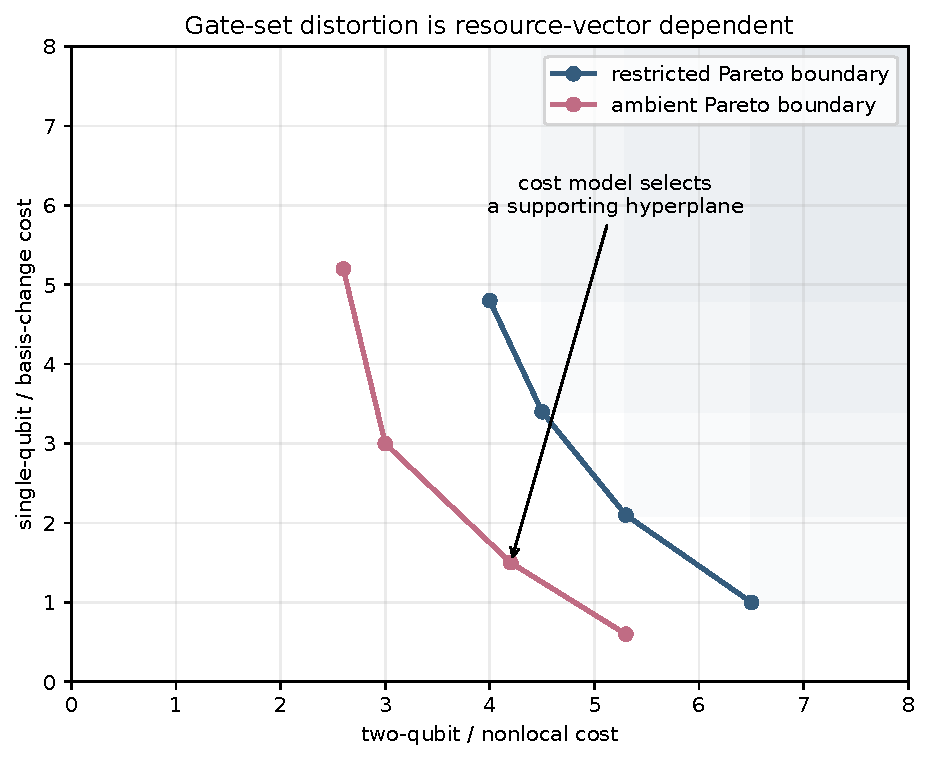
\includegraphics[width=.91\textwidth]{assets/g_resource_pareto.pdf}
\caption{Gate-set defects generally live in a multi-resource Pareto geometry.}
\label{g:fig:resource-pareto}
\end{figure}

\subsection{Depth, count, and space-time volume}
Let $g_t$ be the set of gates scheduled in layer $t$.  Common scalar costs are
\[
\sum_t |g_t|,
\qquad
\#\{t:g_t\ne\varnothing\},
\qquad
\sum_t \#\{\text{active qubits in layer }t\}.
\]
A catalyst may reduce count but increase depth, or vice versa.  Space-time volume is often the more stable hardware quantity.

For stochastic error rates $p_g$, a first-order weighted cost is
\[
C_{\mathrm{err}}(W)=\sum_{g\in W}-\log(1-p_g).
\]
This additive approximation can be inserted directly into Dijkstra search.  It does not capture coherent or correlated errors, but it produces a declared and reproducible metric.

\subsection{Approximate synthesis}
For continuous gate sets, define
\[
\ell_{\mathrm{res},\varepsilon}(U)
=
\min\{\cost(W):\|W-U\|\le\varepsilon\}.
\]
There are two distinct border phenomena:
\begin{enumerate}
\item algebraic border length, where a target lies in the closure of a bounded exact word locus;
\item analytic approximation length, where an error tolerance is explicitly permitted.
\end{enumerate}
They should not be conflated.

A catalyst can improve the asymptotic Solovay--Kitaev or number-theoretic approximation constant even when exact synthesis is impossible in both models.

\subsection{Resource theories and monotones}
A quantum resource theory provides free states, free operations, and monotones.  Gate-set distortion adds a path-sensitive question: the endpoint may be free even though the path temporarily creates resource.

A state monotone $M(\rho)$ alone may fail because the catalyst acts at the channel level.  Useful channel-level quantities include:
\begin{itemize}
\item robustness or magic capacity,
\item entangling power,
\item operator Schmidt rank,
\item Choi-state resource measures,
\item symmetry asymmetry of the channel,
\item amortized resource generation.
\end{itemize}
A lower bound must relate the cumulative or peak resource to the declared gate cost and account for cancellation.

\subsection{A categorical amplification principle}
Suppose a monoidal category admits a tensor product and a cost satisfying
\[
c_{\mathrm{amb}}(f\otimes g)
\le
c_{\mathrm{amb}}(f)+c_{\mathrm{amb}}(g).
\]
If restricted cost is additive on a target family, then any one-copy defect amplifies linearly under independent tensor powers.  Superlinear amplification requires a normalization in which dimensions multiply, as in the matrix tensor rule of the core theory, or a joint-synthesis synergy across copies.

\subsection{Experimental standards}
Every architecture, measurement, or ancilla claim should state:
\begin{enumerate}
\item gate alphabet and native connectivity;
\item clean, dirty, catalytic, or consumable ancilla convention;
\item deterministic or postselected implementation;
\item exact or approximate endpoint condition;
\item total, weighted, depth, or Pareto cost;
\item whether resource-state preparation is included;
\item whether qubit relabeling is free;
\item certificate of restoration on all inputs.
\end{enumerate}
Without these declarations, two reported ``gate counts'' may refer to incomparable problems.

\begin{conjecturebox}
For several common symmetry and architecture restrictions, a constant-size restored excursion should yield an unbounded saving on structured target families.  The unitriangular construction proves this phenomenon for directed linear information flow; analogous theorems for charge sectors, measurement branches, and nonlocal routing remain open.
\end{conjecturebox}

\chapter{Packets, types, holonomy, and restricted realization}
\section{Packets, types, holonomy, and restricted realization}\label{g:ch:packets}
\index{spherical packet}
\index{type packet}
\index{holonomy packet}
\index{realization fiber}
\index{quantum Latin square}
\index{Langlands-style packet}


\subsection{Why coarse spectra are not enough}
A finite symmetry problem often comes with a natural commuting operator algebra.  Its joint spectrum is attractive because it is canonical, compact, and computationally cheap.  Yet the joint eigenvalues and their multiplicities can be identical across objects whose realization behavior is different.

This chapter develops the hierarchy
\begin{equation}\label{g:eq:packet-hierarchy}
\text{spherical packet}
\prec
\text{embedded type packet}
\prec
\text{holonomy packet}
\prec
\text{realization fiber}.
\end{equation}
The relation $\prec$ means ``retains strictly more potentially relevant information,'' not that every refinement is complete.

\begin{figure}[ht]
\centering
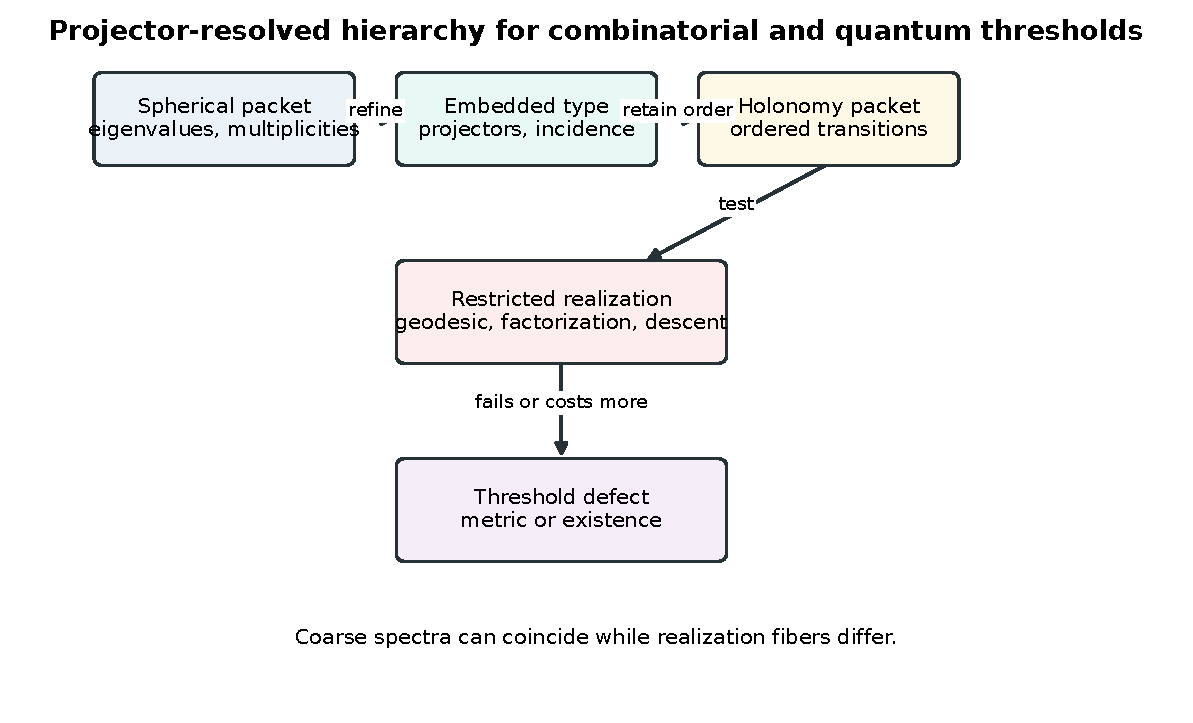
\includegraphics[width=.95\textwidth]{assets/g_packet_hierarchy.pdf}
\caption{The packet hierarchy used to organize finite threshold systems.}
\label{g:fig:packet-realization-hierarchy}
\end{figure}

\subsection{Spherical packets}
Let $T_1,\ldots,T_m$ be commuting normal operators on a finite-dimensional Hilbert space.  Their unique coarsest joint spectral resolution is
\[
T_j=\sum_{\lambda}t_j(\lambda)B_\lambda,
\qquad
\sum_\lambda B_\lambda=I.
\]
The tuple
\[
\lambda=(t_1(\lambda),\ldots,t_m(\lambda))
\]
is the spherical label.  The abstract spectral packet records these labels and the ranks of $B_\lambda$.

Two different embedded systems can have the same abstract packet.  The actual matrices $B_\lambda$, endpoint coefficients, and transition operators may still differ.

\begin{principle}[Spherical collapse]
Passing from embedded operators to eigenvalues and multiplicities can erase exactly the incidence or transition data that controls restricted realization.
\end{principle}

\subsection{The Latin-square association algebra}
A Latin square $L$ of order $n$ has $n^2$ cells.  Let $R,C,S$ be adjacency matrices for equality of row, column, and symbol.  The algebra generated by $I,J,R,C,S$ is commutative and its abstract multiplication table depends only on $n$, not on the paratopy class of $L$.

Define
\[
Q_R=\frac{I+R}{n},
\qquad
Q_C=\frac{I+C}{n},
\qquad
Q_S=\frac{I+S}{n},
\qquad
B_0=\frac{J}{n^2}.
\]
Then the five joint projectors are
\[
B_0,
\quad Q_R-B_0,
\quad Q_C-B_0,
\quad Q_S-B_0,
\quad I-Q_R-Q_C-Q_S+2B_0.
\]
Their multiplicities are
\[
1,
\quad n-1,
\quad n-1,
\quad n-1,
\quad (n-1)(n-2).
\]
The Latin-square graph $R+C+S$ has universal spectrum
\[
3(n-1)^1,
\qquad
(n-3)^{3(n-1)},
\qquad
(-3)^{(n-1)(n-2)}.
\]
At $n=6$ this becomes
\[
15^1,\qquad3^{15},\qquad(-3)^{20}.
\]
Thus the graph spectrum cannot distinguish the twelve main classes of order six.

\begin{provedbox}
The displayed projector formulas depend only on the Latin-square axioms and the order.  They therefore prove that the abstract $R,C,S$ joint eigenvalue packets cannot distinguish squares of the same order.  This conclusion does not require an enumeration of the order-six main classes.
\end{provedbox}

\subsection{Transition fusion also collapses}
Let $\rho_i$ be the row permutations of a Latin square.  The symmetrized aggregate of all pair transitions satisfies
\begin{equation}\label{g:eq:transition-fusion}
\sum_{i<j}
\left(
P_{\rho_i\rho_j^{-1}}
+
P_{\rho_j\rho_i^{-1}}
\right)
=n(J-I).
\end{equation}
Hence first-order fusion destroys the class information as well.

The lesson is general: summing typed transitions can be as destructive as discarding the embedded projectors.  Order and labels matter.

\subsection{Embedded type data}
A type packet retains the actual projectors, support partitions, distinguished incidence sets, or local representation types.  Examples include:
\begin{itemize}
\item the row, column, and symbol partitions of a Latin square;
\item a projective-line closure system;
\item the flag stabilized by a circuit subgroup;
\item support patterns of unitary or quantum-Latin entries;
\item ramification or block data in a finite group action.
\end{itemize}

A projective-line closure procedure can supply additional type operators, such as adjacency operators of a line spread.  Whether a particular added operator separates two classes is a further question.  The present archive does not include the separate order-six projective computation, so it supplies no new finite certification of that comparison.

\subsection{Holonomy packets}
Let a family of local charts or rows be represented by permutations $\rho_i$.  Define normalized transitions
\[
h_{ij}=\rho_i\rho_j^{-1}
\]
and the transition group
\[
H_r(L)=\langle h_{ij}:i,j\rangle.
\]
A holonomy packet may include:
\begin{itemize}
\item the isomorphism type or order of $H_r(L)$,
\item the cycle-type inventory of the distinguished $h_{ij}$,
\item block systems and orbit partitions,
\item characters or matrix coefficients of words in the $h_{ij}$,
\item noncommutative moments
\[
\operatorname{tr}(h_{i_1j_1}\cdots h_{i_kj_k}),
\]
\item the corresponding packets for row, column, and symbol roles.
\end{itemize}

Isotopy conjugates these transition groups; paratopy permutes the three roles.  Therefore the unordered multiset of role signatures is a paratopy invariant.

\begin{skeletonbox}
For a specified collection of Latin squares, one can compute transition-group orders, pair-transition cycle inventories, and nontrivial block sizes, then test whether the resulting role signatures separate the collection.  The separate order-six input tables and verifier are not included in this archive, so pairwise separation of all twelve main classes is an open verification obligation here.
\end{skeletonbox}
Even a complete discrete classification would not prove orthonormal representability.  Noncommutative transition data are candidate refinements of the information lost under spherical fusion.

\subsection{Imprimitivity as hidden decomposition}
A transitive permutation group is imprimitive when it preserves a nontrivial block system.  In combinatorial designs, imprimitivity often signals a subsquare, product, congruence, or module decomposition.

For a Latin square of order $2m$, normalize one row to the identity permutation on the symbols.  An $m\times m$ Latin subsquare determines a partition of the symbols into its $m$ symbols and their complement.  Rows meeting the subsquare preserve the two corresponding column blocks, and the remaining rows exchange them.  Thus normalized row transitions preserve this two-block system.  Conversely, if all normalized row transitions preserve a partition into two blocks of size $m$, exactly $m$ rows send a fixed column block into a fixed symbol block, producing an $m\times m$ Latin subsquare.  This is a structural criterion.  Counting the order-six classes with this property requires separate input representatives.

\begin{principle}[Clifford-type decomposition]
Combinatorial substructure can be detected as imprimitivity of a transition packet.  The spherical packet sees aggregate multiplicities; the holonomy packet sees how those multiplicities are assembled into blocks.
\end{principle}

\subsection{Realization fibers}
Let $P$ denote packet data and let
\[
\operatorname{Real}_{\mathrm{res}}(P)
\]
be the space of restricted realizations compatible with $P$.  The packet may completely classify the discrete object while the realization fiber remains empty, positive dimensional, disconnected, or singular.

Examples of realization conditions include:
\begin{itemize}
\item a flag-preserving geodesic with a declared length;
\item a product-state orthonormal representation;
\item a positive semidefinite Gram matrix with a zero pattern;
\item a tensor factorization;
\item a global descent object compatible with local packets;
\item a circuit satisfying ancilla restoration on every input.
\end{itemize}

Thus classification and realization are distinct layers.

\subsection{Quantum Latin squares as an existence defect}
A quantum Latin square is an array \cite{s:MustoVicary2016} of vectors whose rows and columns are orthonormal bases.  Ball and Simoens prove that a pair of non-entangled mutually orthogonal quantum Latin squares of order six does not exist, while earlier work provides entangled order-six solutions and hence AME$(4,6)$ states \cite{s:BallSimoens2026,s:RatherEtAl2022,g:RatherEtAl2023}.

This is naturally expressed as
\[
\operatorname{Real}_{\mathrm{product}}(P_6)=\varnothing,
\qquad
\operatorname{Real}_{\mathrm{entangled}}(P_6)\ne\varnothing.
\]
It is an existence defect, not a gate-count defect.

\begin{figure}[ht]
\centering
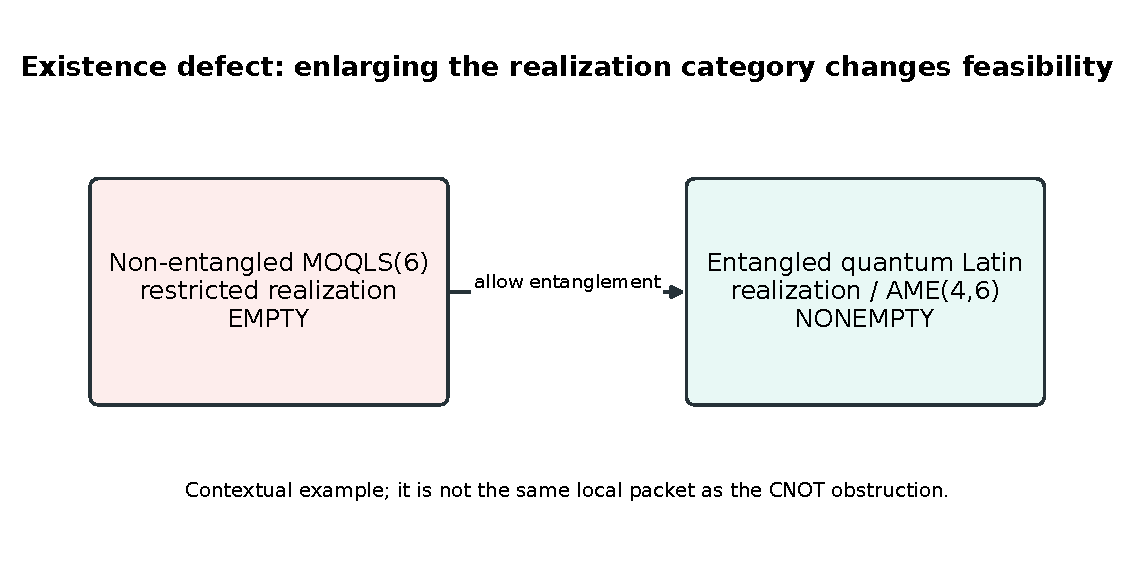
\includegraphics[width=.92\textwidth]{assets/g_quantum_latin_realization_gap.pdf}
\caption{The order-six quantum-Latin distinction is a restricted-versus-ambient realization gap.}
\label{g:fig:quantum-latin-gap}
\end{figure}

The source proof uses support patterns, a reduction to one classical square, orthonormal representations of complements of Latin-square graphs, projective-line closure, finite case analysis over twelve main classes, and a continuous argument for the two remaining subsquare cases.  No theorem in the unitriangular or Clifford chapters is inferred from this result.

\subsection{First-arrival packets}
For a finite generator set $S$, the endpoint Green kernel
\[
\mathcal G_{S,g}(z)
=
\langle\delta_g,(I-zA_S)^{-1}\delta_e\rangle
\]
contains more information than the spectrum of $A_S$.  Its first nonzero degree is the distance to $g$.

If
\[
A_S=\sum_\lambda \lambda B_\lambda,
\]
then
\[
\mathcal G_{S,g}(z)
=
\sum_\lambda
\frac{\langle\delta_g,B_\lambda\delta_e\rangle}{1-\lambda z}.
\]
The endpoint matrix coefficients of the embedded projectors determine cancellation between spectral components.  This is the metric analogue of retaining a type rather than only an unramified eigencharacter.

\subsection{Typed Green kernels}
Let $H\le G$ and let $\mu_k(h)$ count ambient words of length $k$ with holonomy $h\in H$.  For an irreducible representation $\tau$ of $H$, define
\[
\widehat\mu_k(\tau)
=
\sum_{h\in H}\mu_k(h)\tau(h)
\]
and
\[
\widehat{\mathcal G}_\tau(z)
=
\sum_{k\ge0}\widehat\mu_k(\tau)z^k.
\]
Fourier inversion recovers every $\mu_k(h)$.  The trivial representation records only total return to the subgroup; nontrivial types resolve the holonomy.

\begin{provedbox}
For finite $H$, the full family of typed Green kernels over $\widehat H$ determines every endpoint Green series and therefore every ambient word distance from the identity to an element of $H$.
\end{provedbox}

\subsection{Operational Langlands analogy}
The hierarchy resembles the local organization of representation theory:
\[
\text{spherical character}
\to
\text{type}
\to
\text{ramification or monodromy}
\to
\text{realization and descent}.
\]
The analogy is useful because it prevents coarse spectral data from being mistaken for a complete correspondence.  It does not imply that global Langlands reciprocity predicts either the circuit threshold or the quantum-Latin result.

\begin{boundarybox}
The word ``Langlands'' in this monograph refers to an operational packet architecture: commuting local spectra, type refinement, noncommutative holonomy, tensor assembly, and descent obligations.  No general automorphic or Galois correspondence is claimed or used.
\end{boundarybox}

\subsection{A general finite threshold system}
A packet-resolved threshold system consists of:
\begin{enumerate}
\item a finite group, groupoid, or association scheme;
\item a commutative spherical algebra with exact projectors;
\item embedded incidence or type data;
\item a transition group or monodromy representation;
\item restricted and ambient realization categories;
\item a metric, multiplicity, or descent obstruction.
\end{enumerate}

The first threshold may then be defined as
\[
\tau=
\min\{n:\exists P\text{ with }c_{\mathrm{res}}(P)>c_{\mathrm{amb}}(P)\}.
\]
The cost can be finite or infinite.

\subsection{Open problems}
\begin{question}
For which finite association schemes does the full embedded Bose--Mesner algebra determine the restricted realization fiber?
\end{question}
\begin{question}
What bounded degree of noncommutative transition moments separates all Latin squares of a fixed order?
\end{question}
\begin{question}
Can typed Green kernels yield new lower bounds without enumerating the full ambient group?
\end{question}
\begin{question}
When does imprimitivity of a transition packet characterize a tensor or subsquare decomposition in quantum combinatorial designs?
\end{question}

\chapter{The computational atlas and open directions}
\section{The exact computational atlas}\label{g:ch:atlas}
\index{breadth-first search}
\index{zero-one BFS}
\index{Dijkstra algorithm}
\index{certificate}
\index{reproducibility}


\subsection{Purpose and design}
The accompanying code is an audit-oriented finite mathematics package rather than a production compiler.  Its goals are:
\begin{enumerate}
\item exact state representations with no floating-point ambiguity;
\item complete finite search where the state space is tractable;
\item explicit witnesses and reconstructible paths;
\item small, dependency-free core algorithms;
\item frozen JSON results and regression tests;
\item separation between proved, computed, and proposed claims.
\end{enumerate}

The package is named \texttt{catalytic\_gate\_atlas}.  Binary matrices are tuples of integer row bitmasks, and reversible Boolean maps are exact permutations of basis-state indices.

\begin{figure}[ht]
\centering
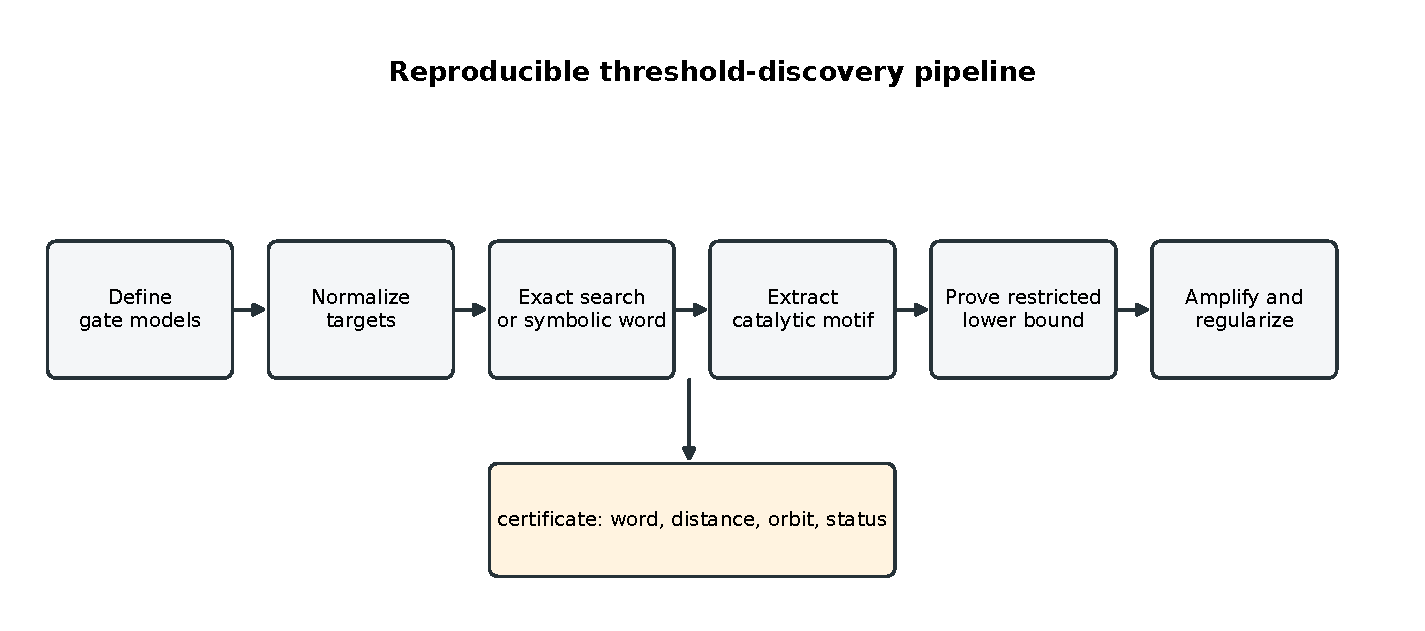
\includegraphics[width=.96\textwidth]{assets/g_computational_pipeline.pdf}
\caption{The finite certificate pipeline used throughout the computational atlas.}
\label{g:fig:computational-pipeline}
\end{figure}

\subsection{State models}
\subsubsection{Binary matrices}
An $m\times m$ matrix over $\F_2$ is stored as
\[
(r_0,\ldots,r_{m-1}),
\]
where bit $j$ of $r_i$ is the $(i,j)$ entry.  Matrix multiplication is exact XOR accumulation.

\subsubsection{Symplectic Clifford states}
An $n$-qubit Clifford modulo global phase and Pauli translation is represented by its action on Pauli exponent vectors
\[
(x\mid z)\in\F_2^{2n}.
\]
The state space is $\Sp(2n,2)$.  The restricted parabolic group is generated by $S$, CZ, and CNOT; the ambient group additionally permits $H$.

\subsubsection{Classical reversible states}
A reversible map on $n$ bits is stored as a permutation of $\{0,\ldots,2^n-1\}$.  Composition is exact.  The affine subgroup is generated by $X$ and CNOT, and the ambient three-bit group adds Toffoli.

\subsection{Shortest-path engines}
The package implements:
\begin{itemize}
\item breadth-first search for unit costs;
\item $0$--$1$ breadth-first search when gates are free or unit cost;
\item Dijkstra search for general nonnegative integer weights;
\item parent maps for witness reconstruction;
\item defect distributions on a restricted target set.
\end{itemize}

\begin{algorithm}[Breadth-first defect census]
Given restricted generators $S_R$, ambient generators $S_A$, and identity $e$:
\begin{enumerate}
\item compute $d_R$ on $\langle S_R\rangle$;
\item compute $d_A$ on $\langle S_A\rangle$;
\item for every restricted state $x$, compare $d_R(x)$ and $d_A(x)$;
\item record the pair $(d_R(x),d_A(x))$ and reconstruct witnesses for strict inequalities.
\end{enumerate}
\end{algorithm}

For a finite group this is complete because every vertex reachable from the identity is visited exactly once at its minimum distance.

\subsection{Zero-cost gates}
When local Clifford gates are free and entangling gates cost one, ordinary BFS is invalid.  The package uses a deque-based $0$--$1$ BFS.  A zero-cost edge is pushed to the front and a unit-cost edge to the back.  The resulting labels are exact shortest entangling costs.

A common error is to quotient by free gates without proving that the quotient preserves the target subset and all left/right actions.  The atlas avoids this issue by running $0$--$1$ BFS directly on the finite group for the reported small cases.

\subsection{The optimized Clifford verifier}
The three-qubit symplectic group has
\[
|\Sp(6,2)|=1{,}451{,}520
\]
states.  A compact C++ implementation enumerates the full group and the parabolic subgroup exactly.  It supports:
\begin{itemize}
\item total primitive count;
\item total count with unit-cost SWAP;
\item entangling count with $H$ and $S$ free;
\item exact distance distributions and JSON output.
\end{itemize}
The C++ program and the independent Python implementation use the same gate matrices but different traversal code.  Witness reconstruction is supplied by the Python implementation, not by the C++ census executable.

\subsection{Computed Clifford census}
\begin{longtable}{@{}ccccccc@{}}
\toprule
$n$ & Metric & SWAP & $|P_n|$ & $|\Sp(2n,2)|$ & Defects & Max defect\\
\midrule
1 & total & no & 2 & 6 & 0 & 0\\
1 & entangling & no & 2 & 6 & 0 & 0\\
2 & total & no & 48 & 720 & 0 & 0\\
2 & entangling & no & 48 & 720 & 4 & 1\\
3 & total & no & 10,752 & 1,451,520 & 24 & 1\\
3 & total & yes & 10,752 & 1,451,520 & 0 & 0\\
3 & entangling & no & 10,752 & 1,451,520 & 1,624 & 2\\
\bottomrule
\end{longtable}

The detailed defect distributions are:
\[
\begin{array}{c|l}
\text{model}&\text{restricted}\to\text{ambient pairs}\\
\hline
n=2\text{ entangling}&3\to2:4\\
n=3\text{ total}&7\to6:6,\quad8\to7:18\\
n=3\text{ entangling}&3\to2:24,\ 4\to3:432,\ 5\to4:1056,\ 6\to4:48,\ 6\to5:64.
\end{array}
\]

\begin{computedbox}
Every entry in the table is a complete finite enumeration in the declared binary symplectic model.  Phases and Pauli translations are not part of the state space.  These are exact results for that quotient model, not full hardware Clifford optimizations.
\end{computedbox}

\subsection{Computed affine-versus-Toffoli census}
For three bits:
\[
|\operatorname{AGL}(3,2)|=1344,
\qquad
|S_8|=40320.
\]
The complete census finds no affine target with a strict defect under total primitive count or under entangling count with NOT free.

\begin{longtable}{@{}ccccc@{}}
\toprule
Metric & Restricted size & Ambient size & Restricted diameter & Defects\\
\midrule
Total & 1,344 & 40,320 & 7 & 0\\
Entangling & 1,344 & 40,320 & 6 & 0\\
\bottomrule
\end{longtable}

\subsection{Linear symbolic checks}
The Python module verifies that the displayed six-row ambient and restricted words produce the same canonical target modulo
\[
2,3,5,8.
\]
The lower bounds and ring universality are proved in the core chapter; these modular checks are regression tests rather than the logical basis of the theorem.

\subsection{Witness format}
A witness record contains:
\begin{itemize}
\item the target matrix or permutation;
\item restricted and ambient costs;
\item a named restricted gate path;
\item a named ambient gate path;
\item the metric and gate alphabet;
\item the state-model convention.
\end{itemize}
For example, the two-qubit entangling Clifford witness has restricted path
\[
\CX_{0\to1},\ S_1,\ \CX_{1\to0},\ \CX_{0\to1}
\]
and ambient path
\[
H_1,\ \CX_{1\to0},\ \CX_{0\to1},\ H_0,\ S_1,\ S_0.
\]
Only two gates in the ambient path are charged by the entangling metric.

\subsection{Certificates beyond full enumeration}
For larger systems, the following certificate styles are supported in principle.
\begin{enumerate}
\item \textbf{Meet in the middle.}  Store forward and backward balls whose radii sum to the candidate length.
\item \textbf{SAT/SMT.}  Encode gate choices and endpoint equations; use an UNSAT certificate below the claimed optimum.
\item \textbf{Integer programming.}  Useful when a fixed gate skeleton leaves discrete routing choices.
\item \textbf{Algebraic elimination.}  Eliminate continuous gate parameters from bounded-length word equations.
\item \textbf{Dual potentials.}  Exhibit a one-Lipschitz potential attaining the claimed lower bound.
\item \textbf{Quotient search.}  Search cosets only after proving that the quotient is compatible with the cost and target class.
\end{enumerate}

\subsection{Multiobjective search}
Let each gate have a vector cost in $\N^r$.  At each state, retain only nondominated labels.  The algorithm terminates for finite state spaces with a bounded search region, but the frontier can grow exponentially.

A practical exact strategy is to scalarize with several positive weight vectors, use the resulting optima to identify candidate Pareto points, and then certify each candidate by constrained search.

\subsection{Reproducibility commands}
From the \texttt{code} directory:
\begin{lstlisting}[style=pythonstyle,caption={Python atlas commands.}]
python -m pip install -e . --no-build-isolation
python scripts/run_atlas.py --output ../results/atlas_small.json
python -m pytest tests
\end{lstlisting}
The optimized three-qubit verifier can be compiled by
\begin{lstlisting}[style=cppstyle,caption={C++ Clifford verifier.}]
g++ -O3 -std=c++20 scripts/clifford_census.cpp -o scripts/clifford_census
./scripts/clifford_census --n 3 --metric total --output ../results/clifford_n3_total.json
./scripts/clifford_census --n 3 --metric entangling --output ../results/clifford_n3_entangling.json
\end{lstlisting}

\subsection{Validation policy}
The release uses four layers of validation.
\begin{enumerate}
\item Unit tests for matrix, permutation, and path primitives.
\item Cross-checks of group sizes against known finite formulas.
\item Independent Python and C++ computations for selected Clifford cases.
\item Frozen JSON outputs and SHA-256 manifests in the release archive.
\end{enumerate}

\subsection{Scaling limits}
Full group enumeration grows rapidly:
\[
|\Sp(2n,2)|
=2^{n^2}\prod_{j=1}^n(4^j-1).
\]
The four-qubit symplectic group is far beyond direct Python BFS.  Future work should exploit:
\begin{itemize}
\item double-coset normal forms,
\item Bruhat or parabolic decompositions,
\item admissible heuristics for A* search,
\item SAT encodings,
\item orbit reduction,
\item tensor-network representations,
\item distributed meet in the middle.
\end{itemize}

\subsection{What the atlas does not prove}
A finite census establishes only the declared finite model.  It does not prove:
\begin{itemize}
\item an asymptotic theorem without a separate proof,
\item a hardware advantage under a different cost,
\item robustness to approximation,
\item equivalence after adding ancillas,
\item a result for global phases or Pauli translations if they were quotiented out.
\end{itemize}
The status metadata in every result file is intended to make these boundaries machine readable.

\section{Reusable theorem templates}\label{g:ch:templates}
\index{theorem template}
\index{lower bound}
\index{dimension per gate}
\index{tensor amplification}


\subsection{Purpose}
This chapter collects proof architectures that recur across gate logics.  Each template separates the easy upper-bound identity from the difficult lower-bound obligation.  The templates are not claims that every gate hierarchy satisfies the hypotheses.

\subsection{Template I: catalytic conjugation}
Let $H\le G$ have restricted and ambient costs with $\ellAmb(g^{-1})=\ellAmb(g)$.  Choose $g\in G$ and $h_1,\ldots,h_m\in H$ such that
\[
U=g h_m\cdots h_1 g^{-1}\in H.
\]
Then
\[
\ellAmb(U)
\le
2\ellAmb(g)+\sum_i\ellAmb(h_i).
\]

\begin{theorem}[Catalytic comparison template]
Assume a restricted lower bound of the form
\[
\ellRes(U)
\ge
\sum_i r_i-\beta,
\]
where $r_i$ is the restricted cost of the $i$th transported obligation and $\beta$ is the maximum certified sharing.  Then
\[
\Delta(U)
\ge
\sum_i r_i-\beta
-
2\ellAmb(g)-\sum_i\ellAmb(h_i).
\]
\end{theorem}

The proof is immediate.  The research content lies in bounding $\beta$.

\subsection{Template II: amortized consumers}
Suppose a catalyst costs $c_{\mathrm{open}}+c_{\mathrm{close}}$ and each of $m$ consumers saves at least $s_i$ restricted cost.  Then
\[
\Delta(U)
\ge
\sum_{i=1}^m s_i
-c_{\mathrm{open}}-c_{\mathrm{close}}-r,
\]
where $r$ is repair or interference cost.  A threshold occurs when the right side first becomes positive.

This template explains the three-cross rule in the linear atom and guides searches in phase, Gaussian, and routing models.

\subsection{Template III: first-arrival Green valuation}
Let $S$ be a finite symmetric generating set and
\[
A_S=\sum_{s\in S}\rho(s).
\]
Then
\[
\mathcal G_{S,g}(z)
=\sum_{k\ge0}\langle\delta_g,A_S^k\delta_e\rangle z^k.
\]

\begin{theorem}[First-arrival template]
If word multiplicities are nonnegative, then
\[
d_S(e,g)=\ord_{z=0}\mathcal G_{S,g}(z).
\]
For restricted and ambient sets,
\[
\Delta(g)=\ord_0\mathcal G_{S_R,g}-\ord_0\mathcal G_{S_A,g}.
\]
\end{theorem}

This template provides an exact spectral restatement.  To turn it into a lower bound without enumeration, one needs control of the endpoint projector coefficients.

\subsection{Template IV: one-Lipschitz potentials}
Let $F$ be a function on circuit states satisfying
\[
F(I)=0,
\qquad
|F(gs)-F(g)|\le c(s)
\]
for every allowed restricted gate $s$.  Then
\[
\ellRes(U)\ge F(U).
\]

Potential design steps:
\begin{enumerate}
\item choose a decomposition into cuts, packets, or degree layers;
\item prove a gate changes the total charge by at most its cost;
\item ensure cancellations cannot create free progress on many layers;
\item evaluate the target exactly.
\end{enumerate}
Static sums of ranks are often too coarse in ambient models; time-expanded or target-relative potentials may be required.

\subsection{Template V: dimension per gate}
Let $X$ be an algebraic family of elementary gates whose irreducible components have dimension at most $r$.  Let $V$ be an irreducible target variety of dimension $N$.

\begin{theorem}[Dimension-per-gate template]
The closure of the locus reachable in $L$ gates has dimension at most $rL$.  If $rL<N$, a generic point of $V$ is not reachable in $L$ gates.
\end{theorem}

If every target in $V$ has a restricted construction of length at most $N/r$, then generic restricted and ambient lengths coincide at that value, provided the same parameter bound applies to the ambient alphabet.

\subsection{Template VI: defect codimension}
Assume every target has restricted cost at most $M$.  A defect of size at least $d$ implies ambient cost at most $M-d$.  If the $(M-d)$-gate ambient locus has dimension at most $N-d$, then
\[
\codim\overline{\mathcal D_{\ge d}}\ge d.
\]
This is the general mechanism behind algebraic rarity.

\subsection{Template VII: finite-field sparsity}
Suppose there are at most $B$ gate directions and at most $q^r$ parameter choices per gate over $\F_q$.  Then the number of words of length at most $L$ is at most
\[
\sum_{j=0}^L(Bq^r)^j.
\]
If the target family has $q^N$ points and defect $d$ forces $L\le (N-d)/r$, this yields a density bound of order $q^{-d}$ up to a fixed combinatorial factor.

The estimate counts words, not distinct endpoints, and is therefore an upper bound without injectivity assumptions.

\subsection{Template VIII: block retraction}
Let a large restricted group contain a smaller one through a homomorphic embedding $\iota$, and suppose a homomorphic retraction $\pi$ satisfies $\pi\iota=\operatorname{id}$.  Require that every large restricted generator maps to a small restricted word of no greater cost.  Then
\[
\ell_{\mathrm{large,res}}(\iota U)
\ge
\ell_{\mathrm{small,res}}(U).
\]
If the ambient embedding preserves gate cost,
\[
\Delta_{\mathrm{large}}(\iota U)
\ge
\Delta_{\mathrm{small}}(U).
\]
This transfers a catalytic atom to architectures containing it as a retract.

\subsection{Template IX: exact block coupling}
For block-lower matrices
\[
M=
\begin{pmatrix}
A&0\\
XA&D
\end{pmatrix},
\]
projection to diagonal blocks forces the costs of $A$ and $D$, while rank of the cross block forces at least $\rank X$ cross transmissions.  If $X$ is a partial monomial matrix, the lower bound is attained by direct construction.

The same logic extends to trees of blocks whenever every coupling layer has an exact rank certificate and the projections are homomorphisms.

\subsection{Template X: tensor Leibniz rule}
Suppose a restricted complexity is tree tight and satisfies
\[
\ellRes(A\otimes B)
=n\ellRes(A)+m\ellRes(B)
\]
for $A$ of size $m$ and $B$ of size $n$.  If ambient complexity satisfies the corresponding upper bound, then
\[
\Delta(A\otimes B)
\ge
n\Delta(A)+m\Delta(B).
\]
For tensor powers,
\[
\Delta(A^{\otimes r})
\ge
r m^{r-1}\Delta(A).
\]
This is the standard route from a finite atom to an $N\log N$ defect.

\subsection{Template XI: stable capacity}
If
\[
a_{r+s}\le m^s a_r+m^r a_s,
\]
then
\[
b_r=\frac{a_r}{m^{r-1}}
\]
is subadditive and
\[
\lim_{r\to\infty}\frac{a_r}{r m^{r-1}}
\]
exists by Fekete's lemma.  This defines a regularized ambient cost and exposes possible tensor activation.

\subsection{Template XII: vector costs}
Let gates carry costs in $\R_+^k$.  A lower bound may be a vector inequality
\[
F(U)\preceq\sum_{g\in W}c(g)
\]
or a family of scalar inequalities indexed by dual weights $w\in\R_+^k$:
\[
w\cdot F(U)\le w\cdot c(W).
\]
A complete Pareto proof may require enough supporting weights to separate the restricted and ambient convex lower hulls.

\subsection{Template XIII: ancilla restoration}
Let $W$ act on data $D$ and ancilla $A$.  To certify a dirty catalyst, prove the operator identity
\[
W=U_D\otimes I_A
\]
on the full joint space, not only on one ancilla input.  For a clean catalyst, prove
\[
W(\ket\psi\otimes\ket0)
=(U\ket\psi)\otimes\ket0
\]
for all $\ket\psi$.  The distinction changes both the target equations and lower bounds.

\subsection{Template XIV: symmetry-sector escape}
Given projectors $P_q$, define off-sector transfer blocks
\[
T_{qr}=P_qUP_r.
\]
A restricted gate preserves all diagonal sectors.  An ambient gate changes a controlled collection of blocks.  A candidate potential is a weighted sum of ranks or norms of obligations relative to the final target.  The proof must charge both creation and useful consumption of off-sector coherence.

\subsection{Template XV: exhaustive threshold classification}
A finite first-threshold theorem should contain:
\begin{enumerate}
\item no defects below size $n_0$;
\item at least one defect at $n_0$;
\item exact classification of every defect at $n_0$ modulo declared equivalence;
\item analytic generation of the exceptional motifs;
\item equality between the analytic set and computational census;
\item witness and completeness certificates.
\end{enumerate}
This is the standard achieved by the six-wire linear core and is the target standard for future gate logics.

\subsection{A proof-obligation ledger}
Before promoting a catalytic identity to a theorem, record:
\begin{longtable}{@{}p{.29\textwidth}p{.62\textwidth}@{}}
\toprule
Obligation & Required evidence\\
\midrule
Endpoint membership & Symbolic proof that the target lies in the restricted class.\\
Ambient upper bound & Explicit circuit evaluated exactly.\\
Restricted lower bound & Potential, rank, algebraic, search, or certificate argument.\\
Restoration & Identity on all data and work inputs under the chosen convention.\\
Cost compatibility & Same gate alphabet, weights, and free operations in both metrics.\\
Minimal threshold & Exhaustive or symbolic exclusion of smaller instances.\\
Equivalence classification & Orbit or normal-form analysis of all minimal defects.\\
Amplification & Proof that the lower bound and upper construction compose.\\
Reproducibility & Source, frozen outputs, and deterministic commands.\\
\bottomrule
\end{longtable}

\section{Research program and paper architecture}\label{g:ch:program}
\index{open problem}
\index{research program}


\subsection{The central research problem}
For a nested pair of gate models, determine the distortion function
\[
D_n=
\sup_{U\in\mathcal T_n}
\bigl(c_{\mathrm{res}}(U)-c_{\mathrm{amb}}(U)\bigr),
\]
where $\mathcal T_n$ is the target class.  The basic questions are:
\begin{enumerate}
\item Does any defect exist?
\item What is the first size threshold?
\item What is the minimal catalytic motif?
\item Is the effect generic, sparse, or confined to special strata?
\item How does it scale under direct sum, recursion, and tensor products?
\item Which resource vector reveals the first defect?
\item Can the effect survive realistic architecture and fault-tolerant costs?
\end{enumerate}

\subsection{Established base camp}
The unitriangular theory provides a complete first example:
\begin{itemize}
\item a universal six-row atom over nonzero commutative rings;
\item exact binary and ternary first-threshold evidence;
\item exact classification of twenty binary minimal defects;
\item connected families with two reverse gates and linear saving;
\item microscopic rank-one, bandwidth-one escape;
\item generic rigidity and defect codimension;
\item recursive and tensor amplification to $\Omega(n\log n)$.
\end{itemize}
The small Clifford atlas adds a second gate logic with genuine exact defects and shows that changing the primitive library by adding SWAP can remove them.

\subsection{Program A: complete the Clifford threshold theory}
The highest-priority quantum project is a paper on parabolic-versus-ambient Clifford synthesis.

\subsubsection{Immediate tasks}
\begin{enumerate}
\item Extend the analytic four-target free-phase orbit certificate to other cost-preserving Clifford equivalences and larger widths.
\item Classify the twenty-four three-qubit total-count defects under parabolic conjugation and qubit permutations.
\item Derive analytic normal forms for the witness circuits.
\item Prove lower bounds independent of full group enumeration.
\item Test depth, weighted, and architecture-aware metrics.
\item Determine whether a finite defective atom tensor-amplifies.
\end{enumerate}

\subsubsection{Longer-term questions}
\begin{conjecture}
The parabolic subgroup of $\Sp(2n,2)$ has unbounded additive distortion in the full symplectic group for at least one natural Clifford cost model.
\end{conjecture}
\begin{question}
Does the maximum total-count defect grow as $n$, $n\log n$, or faster?
\end{question}
\begin{question}
Is the disappearance of three-qubit defects after adding unit-cost SWAP a small-width accident or a structural geodesic-convexity phenomenon?
\end{question}

\subsection{Program B: temporary nonlinearity}
The three-bit affine-versus-Toffoli census is rigid.  The next target is a complete four-bit normal-form search without enumerating $16!$ permutations.

\subsubsection{Algorithmic plan}
\begin{enumerate}
\item Compute exact affine distances for all $|\operatorname{AGL}(4,2)|=322{,}560$ targets.
\item Enumerate Toffoli sandwiches modulo affine left and right actions.
\item Use ANF equations to retain only affine endpoints.
\item Compare total, Toffoli, CNOT, and fault-tolerant costs.
\item Produce SAT certificates below every claimed optimum.
\end{enumerate}

\begin{question}
What is the first bit width at which a restored nonlinear excursion shortens an affine target?
\end{question}
\begin{question}
Can temporary degree two yield a family with unbounded saving while the endpoint degree remains one?
\end{question}

\subsection{Program C: phase-polynomial catalysts}
The phase setting is likely to produce a defect first in a resource other than total primitive count.

Priority metrics:
\[
T\text{-depth},
\quad
\text{CNOT count at fixed }T\text{-count},
\quad
\text{two-qubit depth},
\quad
\text{architecture-weighted cost}.
\]
A first paper should choose one metric and avoid a diffuse comparison across all resources.

\begin{question}
Can a restored Hadamard or Clifford frame reduce $T$-depth of a diagonal target without additional ancillas?
\end{question}
\begin{question}
Does tensor activation occur for phase-polynomial $T$-count?
\end{question}

\subsection{Program D: Gaussian and matchgate systems}
Two concrete first searches are recommended.
\begin{enumerate}
\item Number-conserving versus general fermionic Gaussian synthesis on a small number of modes.
\item Nearest-neighbor versus all-to-all matchgate circuits with weighted fermionic SWAP cost.
\end{enumerate}
Both admit exact orthogonal-matrix representations and have clear architecture relevance.

\subsection{Program E: symmetry and measurement}
This program should begin with a narrowly declared resource theory, such as:
\begin{itemize}
\item excitation-preserving two-qubit gates versus arbitrary two-qubit gates;
\item unitary Clifford+$T$ versus measurement-assisted Clifford+$T$;
\item clean versus dirty ancillas for a fixed arithmetic family;
\item local architecture versus one reusable nonlocal bus gate.
\end{itemize}
The first objective is not maximal generality but one theorem with exact restoration and cost accounting.

\subsection{Program F: root-system catalysis}
For a split reductive group with allowed roots $\Psi\subset\Phi$, classify configurations in which a forbidden root acts as a reusable catalyst through Chevalley commutator relations.

Suggested sequence:
\[
A_2\to B_2=C_2\to G_2\to A_r.
\]
Low-rank nonsimply laced systems are attractive because longer root strings may create more than one useful effect per consumer.

\begin{question}
Is there a root-system analogue of the three-cross, one-phase threshold?
\end{question}
\begin{question}
Can a $G_2$ root string produce a multiplicative distortion exceeding the clean type-$A$ value $3/2$?
\end{question}

\subsection{Program G: algebraic defect loci}
For each finite-dimensional gate hierarchy, define bounded word loci and defect strata.  Determine:
\begin{itemize}
\item irreducible components,
\item exact dimension and codimension,
\item singularities and degenerations,
\item border length,
\item finite-field point counts,
\item behavior under tensor products.
\end{itemize}

\begin{conjecture}
In a broad class of one-parameter elementary gate varieties, defect at least $d$ is generically a codimension-at-least-$d$ condition, with equality on explicit families of components.
\end{conjecture}

\subsection{Program H: packet-resolved realization}
The packet hierarchy should be developed as a separate mathematical framework rather than appended to every circuit paper.

Core objectives:
\begin{enumerate}
\item define spherical, type, and holonomy functors for finite transition groupoids;
\item prove information-loss theorems for commutativization;
\item classify when typed Green kernels are sufficient for distance;
\item relate imprimitivity to combinatorial decomposition;
\item formalize realization fibers and descent obstructions.
\end{enumerate}

\subsection{Recommended paper sequence}
\begin{longtable}{@{}>{\raggedright\arraybackslash}p{.08\textwidth}>{\raggedright\arraybackslash}p{.37\textwidth}>{\raggedright\arraybackslash}p{.45\textwidth}@{}}
\toprule
Paper & Working title & Core result\\
\midrule
I & Catalytic escape from unitriangularity & Completed linear threshold, rarity, and asymptotic distortion.\\
II & Catalytic basis escape in Clifford synthesis & Exact parabolic-versus-Clifford thresholds and analytic motifs.\\
III & Temporary nonlinearity in reversible circuits & Affine targets with or without Toffoli-assisted defects.\\
IV & Gate-set distortion and catalytic holonomy & Abstract subgroup, groupoid, and vector-cost theory.\\
V & Spherical collapse and transition holonomy & Packet refinement, Latin-square holonomy, and realization fibers.\\
VI & Algebraic defect loci & Word varieties, codimension, border catalysis, and point counts.\\
VII & Root-system catalytic complexity & Chevalley commutators and thresholds beyond type $A$.\\
\bottomrule
\end{longtable}

\subsection{Software roadmap}
Version $0.1$ of the atlas supports exact small finite groups.  A mature package should add:
\begin{enumerate}
\item generic multiobjective Dijkstra search;
\item disk-backed and parallel BFS;
\item SAT and SMT export;
\item group action and orbit classification;
\item symbolic word-map elimination;
\item circuit diagrams in Quantikz and SVG;
\item architecture graphs and routing costs;
\item certificate verification independent of the search engine;
\item a machine-readable theorem-status ledger.
\end{enumerate}

\subsection{Standards for claims}
A result should be labeled \emph{proved} only when every lower bound and restoration claim has a proof.  A complete finite census should identify the state quotient, enumerate its full size, and make the traversal reproducible.  A symbolic skeleton should be valued as a research object but not described as an established shortcut.

\subsection{Potential applications}
If developed, the theory may contribute to:
\begin{itemize}
\item exact and heuristic quantum circuit compilers,
\item architecture-aware routing,
\item parity and phase-network synthesis,
\item stabilizer and Clifford optimization,
\item reversible arithmetic,
\item Gaussian and fermionic simulation,
\item lower-bound methodology,
\item geometric group theory of gate sets,
\item algebraic geometry of circuit word maps.
\end{itemize}
The near-term value is methodological and algorithmic.  Hardware benefit requires a device-specific cost and noise model.

\subsection{Twenty central open problems}
\begin{enumerate}
\item Prove or refute a universal six-dimensional linear threshold over all coefficient rings.
\item Determine the true asymptotic order of the maximum unitriangular defect.
\item Decide whether multiplicative distortion is bounded.
\item Determine the lower border length of the canonical six-row atom.
\item Classify tree-tight catalytic matroids.
\item Find a one-copy rigid target with tensor activation.
\item Extend the two-qubit analytic orbit certificate to larger Clifford systems.
\item Analytically classify the three-qubit total-count Clifford defects.
\item Determine whether SWAP restores rigidity for all $n$ in the chosen primitive model.
\item Find the first affine target shortened by temporary nonlinearity, or prove none exists.
\item Find the first diagonal target improved by non-diagonal Clifford catalysis.
\item Determine a phase-polynomial Pareto defect.
\item Find a number-conserving Gaussian target shortened by Bogoliubov escape.
\item Find a matchgate routing catalyst with a certified architecture advantage.
\item Establish a symmetry-sector microscopic-escape theorem.
\item Classify when a fixed number of dirty ancillas gives unbounded saving.
\item Develop typed Green-kernel lower bounds that avoid full enumeration.
\item Determine finite moment bounds sufficient for transition-holonomy classification.
\item Classify catalytic motifs in $B_2$, $C_2$, and $G_2$.
\item Prove a general theorem connecting algebraic codimension and catalytic defect.
\end{enumerate}

\subsection{Closing perspective}
The common phenomenon is not that every restriction can be beaten.  It is that the path space matters.  A target may obey a symmetry, flag, degree bound, locality rule, or factorization constraint while the cheapest route to that target does not.

The disciplined research question is therefore:
\begin{center}
\fbox{\parbox{.90\textwidth}{\centering
Which temporary resources can be opened, reused, and exactly removed at a net computational gain?}}
\end{center}
The established linear theory answers this question completely for one important model.  The monograph supplies the symbolic and computational machinery to ask it across quantum gate logic without conflating identities, experiments, and theorems.


\endgroup
\VolumePart{Circuit obstructions}
{Restored reversible circuits lead to cut comparisons, safe discrepancy covers, and projection costs. The later chapters examine faithful linear summaries and the obstruction to composing multiplicative descriptions.}
{
\VolumePartEntry{13}{Scope, notation, and computational model}
\VolumePartEntry{14}{Exact cut comparison and safe discrepancies}
\VolumePartEntry{15}{Complete safe-packet degree}
\VolumePartEntry{16}{Calibration families and exact small oracles}
\VolumePartEntry{17}{Homogeneous projection: cost and safety}
\VolumePartEntry{18}{Faithful linear gluing algebras}
\VolumePartEntry{19}{Weighted witness fingerprints}
\VolumePartEntry{20}{The overlap obstruction to composition}
\VolumePartEntry{21}{Circuit examples in view}
}
\begingroup\renewcommand{\F}{\mathbb F_2}
\renewcommand{\B}{\{0,1\}}
\providecommand{\Aff}{\operatorname{Aff}}
\providecommand{\supp}{\operatorname{supp}}
\providecommand{\Span}{\operatorname{span}}
\providecommand{\KTop}{\operatorname{Top}}
\providecommand{\KTr}{\operatorname{Tr}}
\providecommand{\KTrest}{T_{\mathrm{rest}}}
\providecommand{\MC}{M}
\providecommand{\pathref}[1]{\texttt{\small\detokenize{#1}}}
\chapter{Scope, notation, and computational model}
\label{c:ch:foundations}
\section{Boolean and algebraic conventions}
A Boolean function is a map $f:\B^n\to\B$. Unless a different field is explicitly stated, polynomials are the unique multilinear representatives in
\[
\mathcal R_n=\F[x_1,\ldots,x_n]/(x_i^2-x_i:1\le i\le n).
\]
Addition in this ring is XOR. Multiplication is AND. Boolean OR is written $\lor$ and satisfies $a\lor b=a+b+ab$. A statement $h\le f$ is pointwise and means that $h$ has no positive value at a negative input of $f$.

The degree of a nonzero function is its multilinear algebraic degree. A nonzero constant has degree zero. For mathematical statements involving a constant-zero function we use $\deg0=-\infty$; stored profile tables and Python helpers use their documented sentinels instead. Those implementation conventions do not change the inequalities.

For $S\subseteq[n]$, write $x^S=\prod_{i\in S}x_i$ and let $1_S$ be the input with support $S$. A minterm of a monotone function means an inclusion-minimal positive support, not an arbitrary positive input.

\begin{longtable}{@{}>{\RaggedRight\arraybackslash}p{1.1in}>{\RaggedRight\arraybackslash}p{5.0in}@{}}
\toprule
\textbf{Symbol} & \textbf{Meaning}\\\midrule\endhead
$C(f)$ & Minimum fan-in-two AND/OR/NOT gate count, allowing fan-out.\\
$L(f)$ & Minimum total NOT/CNOT/Toffoli count of a restored implementation.\\
$T$ & Number of Toffoli gates in a specified implementation.\\
$\KTrest(f)$ & Minimum such Toffoli count, allowing any finite zero workspace.\\
$M(f)$ & Minimum AND count in an XOR--AND computation, with affine operations uncharged.\\
$I_f$ & Boolean functions supported only on positive inputs of $f$.\\
$\alpha_1(f)$ & Minimum degree of one nonzero member of $I_f$.\\
$\beta_v(f)$ & Minimum degree of a member of $I_f$ that is one at $v$.\\
$\beta(f),\beta^*(f)$ & Complete-cover degree and its affine-output optimization.\\
$[P]_2$ & Homogeneous degree-two component of the multilinear polynomial $P$ in the specified coordinates.\\
\bottomrule
\end{longtable}

\section{The restored classical oracle}
A legal NOT changes one target bit. A CNOT adds a control bit to a distinct target. A Toffoli adds the product of two distinct controls to a third distinct wire. Gates have positive controls and are self-inverse. Their composition is a permutation of all register states.

A restored oracle is a circuit satisfying
\begin{equation}\label{c:eq:oracle}
(x,0^a,y)\longmapsto(x,0^a,y+f(x))
\end{equation}
for every logical input $x$ and both initial target values $y\in\B$. The zero-workspace condition is imposed at the boundary, not at intermediate times. The circuit may disturb logical inputs, use output feedback, reuse intermediate values, and make arbitrary reversible excursions before restoring the required registers.

NOT and CNOT are free only when counting $T$. They are charged in $L$. This distinction is essential in the projection example. There are no measurements, quantum phases, discarded work registers, or unverified ancilla initializations in this model.

\section{Comparison with ordinary circuits}
\begin{theorem}[Classical/restored simulation comparison]\label{c:thm:simulation}
For every Boolean function $f$,
\[
\frac{C(f)}5\le L(f)\le6C(f)+1.
\]
\end{theorem}
\begin{proof}
Compute every Boolean gate onto a fresh zero wire. An AND costs one Toffoli. A NOT of an existing signal is obtained with one NOT and one CNOT. An OR is computed as $a+b+ab$, using two CNOTs and one Toffoli. Repeated operands are simplified to a copy, not encoded as an illegal repeated-control gate. Compute the output, copy it to $y$, and reverse the first computation. This uses at most $6C(f)+1$ gates and restores every work register.

Conversely, express each reversible gate as an ordinary Boolean update. XOR has a four-gate AND/OR/NOT realization. A Toffoli needs that XOR plus one AND, hence at most five gates. Substitute zero for initial ancillas and $y=0$, then read the final target. The resulting Boolean circuit has at most $5L(f)$ gates.
\end{proof}

\section{The degree bound used throughout}
\begin{lemma}[Degree per multiplication]\label{c:lem:degree}
An XOR--AND computation with $t$ AND gates has output degree at most $t+1$, allowing constants and arbitrary sharing. The same bound holds for each coordinate of a reversible computation containing $t$ Toffoli gates.
\end{lemma}
\begin{proof}
Introduce a formal Boolean variable for each AND output. Its defining expression is a product of two affine forms in the logical inputs and earlier gate variables. The final output is affine in the inputs and all gate variables.

Substitute the gate variables in reverse topological order. A multilinear monomial contains the variable being replaced at most once. Replacing it by a quadratic expression raises degree by at most one; multilinear reduction cannot raise it. After $t$ substitutions the degree is at most $t+1$.

A Toffoli contributes one multiplication to such a straight-line computation, while NOT and CNOT are affine. The argument also applies to a suffix executed backwards because the gates are self-inverse.
\end{proof}
The source identifies this standard degree bound with the XOR--AND background in \cite{c:soeken}.


\section{A degree invariant that retains sharing}
The preceding Boolean substitution proof applies to general XOR--AND straight-line computations. The later formal development proves the classical reversible specialization directly on the evolving register state. This route makes the resource accounting visible without unfolding reused registers into duplicated formulas.

\begin{theorem}[Register-product degree invariant]\label{c:thm:register-products}
Let $s_i(x)$ be the contents of a finite register after $t$ Toffoli gates, with arbitrary intervening NOT and CNOT gates. Initial register contents are affine functions of $x$. For every finite list $L$ of $r$ register indices, including repeated indices,
\[
 \deg\left(\prod_{i\in L}s_i(x)\right)\le t+r.
\]
The zero-function convention is as above. In the formal source the conclusion is the concrete representation certificate \texttt{DegreeLE}.
\end{theorem}
\begin{proof}
Initially a product of $r$ affine functions has degree at most $r$. Suppose a gate toggles register $u$ by a product of $q$ controls, with $q=0,1,2$ for NOT, CNOT, and Toffoli respectively. If $u$ does not occur in $L$, the product is unchanged. If it occurs, Boolean idempotence removes all its repetitions. Let $R$ be the remaining list, so $|R|+1\le r$. The updated product is
\[
 s_u\prod_{i\in R}s_i+
 \left(\prod_{j\in\mathrm{controls}}s_j\right)\prod_{i\in R}s_i.
\]
By the old invariant, these two summands have degrees at most $t+1+|R|$ and $t+q+|R|$. The latter is at most $t+r+\max\{q-1,0\}$. NOT and CNOT therefore consume no degree budget; a Toffoli consumes at most one. Induction along the actual gate list proves the claim. The empty list is the constant-one product and is also covered.
\end{proof}
For $r=1$ this recovers the coordinate bound. The initial target can be fixed to either boundary bit while the inputs vary. Temporary input disturbance, dirty intermediate workspace, output controls, and repeated use of earlier products are all allowed. The formal locators are \texttt{workspaceDegree\_run} and \texttt{canonical\_run\_coordinate\_degree}.

\begin{circuitscopebox}{The representation is part of the theorem}
\texttt{DegreeLE(d,f)} is tied by proved equivalences to an explicit finite XOR of monomials with length at most $d$. It is not an assumed degree oracle. Canonical algebraic-normal-form extraction and a separate generic XOR--AND simulation compiler are outside this formal block.
\end{circuitscopebox}

\chapter{Exact cut comparison and safe discrepancies}
\label{c:ch:cut}\claim{C01}
\begin{theorem}[Cut-comparison identity and complete coverage]\label{c:thm:cut}
Let a restored oracle be written $\mathcal C=Q\circ P$, and put $R=Q^{-1}$. Suppress zero ancillas in boundary arguments and define
\[
 A(x)=P(x,0),\qquad B(x)=R(x,0),\qquad
 D(x)=P(x,1)+P(x,0).
\]
These are vectors indexed by all registers. Then
\begin{equation}\label{c:eq:cut}
 A(x)+B(x)=f(x)D(x),\qquad D(x)\ne0.
\end{equation}
Consequently, the coordinate discrepancies $H_i=A_i+B_i$ satisfy
\begin{equation}\label{c:eq:cover}
 H_i\le f\quad\hbox{for every }i,\qquad
 \bigvee_iH_i=f.
\end{equation}
\end{theorem}
\begin{proof}
For a boundary state with target $z$, correctness of the full circuit gives
\[
 R(x,z)=P(x,z+f(x)).
\]
When $f(x)=0$, this says $B(x)=A(x)$. When $f(x)=1$, it says $B(x)=P(x,1)$, and the discrepancy is $D(x)$. Both cases are summarized by \eqref{c:eq:cut}.

The prefix $P$ is a permutation. Its images of the two distinct boundary states $(x,0)$ and $(x,1)$ are different, so $D(x)$ is a nonzero vector.

If $f(x)=0$, every discrepancy is zero. If $f(x)=1$, at least one discrepancy is one. These are precisely the safety and complete-coverage assertions in \eqref{c:eq:cover}.
\end{proof}

\section{What the comparison does and does not require}
The suffix need not reverse the prefix. Output feedback and a target direction distributed among many registers are permitted. Only boundary correctness and reversibility are used. Equivalently,
\[
 f(x)=1\quad\Longleftrightarrow\quad P(x,0)\ne Q^{-1}(x,0).
\]
This is a necessary representation, not a circuit lower bound from packet count. Expanded monomial counts, individual degrees, and algebra dimensions remain distinct from the shared cost of constructing the complete family. The declared finite cut checks are reported in Section~\ref{c:app:evidence}.

\chapter{Complete safe-packet degree}
\label{c:ch:degree}\claim{C02}
\section{Pointwise coverage rather than one easy packet}
Let
\[
 I_f=\{h\in\mathcal R_n:h(1+f)=0\}.
\]
This is the ideal of functions supported only on the accepting set of $f$. For nonzero $f$, the one-packet parameter is
\[
 \alpha_1(f)=\min\{\deg h:0\ne h\in I_f\}.
\]
It asks for one safe nonzero polynomial, which may detect only an easy portion of the accepting set. One-sided polynomial immunity is established terminology in this setting; see the background reference \cite{c:beckli}.

For a positive input $v$, define instead
\[
 \beta_v(f)=\min\{\deg h:h\in I_f,\ h(v)=1\},\qquad
 \beta(f)=\max_{v:f(v)=1}\beta_v(f).
\]
Set $\beta(0)=0$. Thus $\beta(f)$ is the degree needed before safe polynomials collectively detect \emph{every} positive input. Finally, put
\[
 \beta^*(f)=\max_{\ell\in\Aff_n}\beta(f+\ell),
\]
where $\Aff_n$ is the set of affine Boolean functions on the logical inputs.

\begin{proposition}[Basic size bounds]\label{c:prop:beta-bounds}
For nonzero $f$ on $n$ inputs,
\[
 \alpha_1(f)\le\beta(f)\le n.
\]
If $f$ has at least two positive inputs, then $\beta(f)\le n-1$. In particular $\beta^*(f)\le n$.
\end{proposition}
\begin{proof}
Any polynomial detecting a specified positive input is nonzero, giving the first inequality. For $v\in\B^n$, its point indicator is
\[
 \delta_v(x)=\prod_{i:v_i=1}x_i\prod_{i:v_i=0}(1+x_i).
\]
If $f(v)=1$, then $\delta_v\in I_f$ and has degree $n$, proving the upper bound.

If $v$ and $w$ are distinct positive inputs, $\delta_v+\delta_w$ is safe and equals one at $v$. The degree-$n$ coefficients of its two summands are both one, so they cancel. Its degree is at most $n-1$. Do this for each positive $v$. The last assertion applies the general bound to every affine adjustment, with the stated zero convention.
\end{proof}

\begin{proposition}[Affine input invariance]\label{c:prop:affine-invariance}
Invertible affine changes of logical input coordinates preserve $\alpha_1$, $\beta$, and $\beta^*$, with the pointwise parameters transported by the corresponding bijection of inputs.
\end{proposition}
\begin{proof}
Composition with an affine map cannot increase multilinear degree. Composition with its affine inverse proves equality of degrees. Such composition bijects the accepting and rejecting inputs, hence maps safe polynomials bijectively to safe polynomials and preserves their pointwise detecting property. It also permutes the affine output masks used in the definition of $\beta^*$.
\end{proof}

\section{The restored lower bound}
\begin{theorem}[Affine-optimized complete-cover bound]\label{c:thm:complete-bound}
Every restored implementation of $f$ with $T$ Toffoli gates satisfies
\begin{equation}\label{c:eq:complete-bound}
 T\ge\max\{0,\ \deg f-1,\ 2\beta^*(f)-3\}.
\end{equation}
In particular,
\[
 T\ge\max\{0,\ \deg f-1,\ 2\beta(f)-3,\ 2\beta(1+f)-3\}.
\]
\end{theorem}
\begin{proof}
Cut the implementation after $\lfloor T/2\rfloor$ Toffolis. The forward prefix and the inverse suffix use at most $\lceil T/2\rceil$ Toffolis each. By Lemma~\ref{c:lem:degree}, each of their coordinates, and therefore each discrepancy $H_i$, has degree at most
\[
 \left\lceil\frac T2\right\rceil+1.
\]
Theorem~\ref{c:thm:cut} gives $H_i\le f$ and a complete cover of the positive inputs. Every positive $v$ is therefore detected by a safe polynomial within this degree bound, so
\[
 \beta(f)\le\left\lceil\frac T2\right\rceil+1.
\]
Integer rounding gives $T\ge2\beta(f)-3$.

At the end of a restored oracle the logical inputs are available unchanged. CNOTs from those inputs and, when needed, a target NOT append any affine $\ell$ to the target at no Toffoli cost. Apply the same inequality to each $f+\ell$ and maximize. Finally, reading the target with initial value zero computes $f$ using $T$ multiplications, so Lemma~\ref{c:lem:degree} gives $T\ge\deg f-1$.
\end{proof}

\begin{circuitscopebox}{Scope of the lower bound}
The circuit may use output feedback and arbitrary dirty intermediate states, but it must satisfy the restored classical oracle convention. The inequality does not apply automatically to a model with discarded garbage or measurement. Because $\beta^*(f)\le n$, this parameter alone cannot prove a superpolynomial lower bound in the actual input length.
\end{circuitscopebox}

\section{Exact evaluation-span certificates}
For an integer $d\ge0$, form the evaluation vector
\[
 v_d(x)=\bigl(x^S\bigr)_{S\subseteq[n],\ |S|\le d},
\]
and write $U=f^{-1}(0)$.

\begin{theorem}[Dual certificate for failure of safe detection]\label{c:thm:dual}
For every positive input $v$,
\begin{equation}\label{c:eq:dual}
 \beta_v(f)>d
 \quad\Longleftrightarrow\quad
 v_d(v)\in\Span_{\F}\{v_d(u):u\in U\}.
\end{equation}
\end{theorem}
\begin{proof}
A degree-at-most-$d$ polynomial is a coefficient covector on the evaluation space. It is safe exactly when it annihilates every negative evaluation vector, equivalently their span. Such a covector can equal one on $v_d(v)$ exactly when $v_d(v)$ lies outside that span. This is finite-dimensional linear duality over $\F$.
\end{proof}

\begin{corollary}[Finite support of a dual witness]\label{c:cor:dual-witness}
When the right side of \eqref{c:eq:dual} holds, there is $W\subseteq U$ with
\[
 v_d(v)=\sum_{u\in W}v_d(u),\qquad
 |W|\le\sum_{j=0}^{\min(d,n)}\binom nj.
\]
The cardinality $|W|$ is odd.
\end{corollary}
\begin{proof}
Choose a basis of the span from negative evaluation vectors and express $v_d(v)$ in that basis. Over $\F$, the nonzero coefficients select a subset $W$ of size at most the ambient dimension. The constant-monomial coordinate of every evaluation vector is one; comparing it on both sides shows that $|W|$ is odd.
\end{proof}
Such a relation is replayable by exact linear arithmetic. It does not provide an efficient way to enumerate all negatives of an arbitrary SAT verifier. The theorem assumes that the negative vectors or their proved structure are available.

\section{Monotone specialization}
\begin{theorem}[Safe monomial ideal for a monotone function]\label{c:thm:monotone}
If $f$ is monotone, $I_f$ has a monomial basis indexed by the positive supports of $f$. For each positive $v$,
\[
 \beta_v(f)=\min\{|S|: S\subseteq\supp(v),\ f(1_S)=1\}.
\]
Consequently, for nonzero $f$,
\[
 \alpha_1(f)=\text{minimum minterm size},\qquad
 \beta(f)=\text{maximum minterm size}.
\]
\end{theorem}
\begin{proof}
For any Boolean polynomial $h$, its coefficient on $x^S$ is
\[
 [x^S]h=\sum_{T\subseteq S}h(1_T)
\]
over $\F$. If $S$ is negative for monotone $f$, every subset $T$ is negative. A safe $h$ vanishes at each $1_T$, so its $x^S$ coefficient is zero. Conversely, a monomial on a positive support is safe by monotonicity. This proves the basis assertion.

If a safe $h$ satisfies $h(v)=1$, at least one of its nonzero monomials is supported inside $\supp(v)$. That support is positive and has size at most $\deg h$. Conversely, a smallest such positive-support monomial detects $v$. This proves the pointwise formula. Taking the appropriate minima and maxima gives the minterm statements: a minimal positive support cannot contain a smaller positive one, and every positive input contains a minterm.
\end{proof}

\begin{corollary}[Exact monomial oracle cost]\label{c:cor:monomial}
For $k\ge2$,
\[
 \KTrest(x_1x_2\cdots x_k)=2k-3.
\]
\end{corollary}
\begin{proof}
The unique positive input of the $k$-variable monomial needs a safe polynomial of degree $k$. The complete-cover lower bound gives $2k-3$. For the matching construction, successively compute $x_1x_2$, then $x_1x_2x_3$, and so on up to a $(k-1)$-fold product on clean work wires. Toggle the output using that product and $x_k$, then uncompute the $k-2$ work products. The count is $(k-2)+1+(k-2)=2k-3$. For $k=2$, a single Toffoli suffices.
\end{proof}

\chapter{Calibration families and exact small oracles}
\label{c:ch:calibration}\claim{C03 and C04}
\section{An unbalanced disjunction}
For $k\ge2$ and $n=k+2$, define
\[
 B=z_1\cdots z_k,\qquad
 F_k(a,b,z)=(ab)\lor B=ab+B+abB,\qquad G_k=F_k+a.
\]
This is a deliberately easy family with two differently sized accepting regions. It separates the cost of finding one safe packet from the degree needed for complete coverage.

\begin{proposition}[Raw calibration parameters]\label{c:prop:raw-family}
For this family,
\[
 \alpha_1(F_k)=2,\qquad\beta(F_k)=k,\qquad\deg F_k=k+2.
\]
\end{proposition}
\begin{proof}
The minterms have supports $\{a,b\}$ and $\{z_1,\ldots,z_k\}$. The first two assertions follow from Theorem~\ref{c:thm:monotone}. The monomial $abB$ has degree $k+2$ and does not cancel with either lower-degree term in the displayed polynomial.
\end{proof}

\begin{theorem}[Affine optimization of the one-packet parameter]\label{c:thm:family-alpha}
For every $k\ge2$,
\[
 \max_{\ell\in\Aff_n}\alpha_1(F_k+\ell)=3.
\]
\end{theorem}
\begin{proof}
First restrict to the face $z_1=0$. There $F_k+\ell$ becomes $ab+\ell|_{z_1=0}$, a nonzero quadratic. If the restricted affine term contains a remaining $z$ variable, set $a=0$ and set the remaining affine form to one. This gives an accepting affine subspace of codimension at most two inside the face. If it contains no remaining $z$ variable, fix $a,b$ to an accepting pair instead. The indicator of the resulting affine subspace in the full input space has degree at most three and is safe. Thus every affine adjustment has a nonzero safe polynomial of degree at most three.

For equality, take $\ell=a$. The degree-three polynomial
\[
 a(1+b)(1+z_1)
\]
is safe for $G_k$. Suppose a safe $h$ of degree at most two existed. On $a=0$, acceptance requires $B=1$. For $k\ge3$, the monotone-ideal argument forces $h|_{a=0}=0$, hence $h=aL$ with $L$ affine in the remaining variables. The negative face $a=b=1$ forces $L(1,z)=0$, so $L=c(1+b)$. The negative point $a=1,b=0,z=(1,\ldots,1)$ then forces $c=0$.

When $k=2$, the restriction can initially be $h|_{a=0}=cB$. Write $h=cB+aL$. On the same negative face $a=b=1$, the quadratic term $cB$ cannot be cancelled by affine $L$, so $c=0$. The previous argument then applies. There is no nonzero safe polynomial of degree at most two, proving equality.
\end{proof}

\begin{theorem}[Affine optimization of complete coverage]\label{c:thm:family-beta}
For every $k\ge2$,
\[
 \beta^*(F_k)=k+1.
\]
\end{theorem}
\begin{proof}
Restrict $G_k=F_k+a$ to $b=1$. Then
\[
 G_k|_{b=1}=(1+a)B.
\]
This is the indicator of one point on $k+1$ variables. At the positive input $a=0,b=1,z=(1,\ldots,1)$, a safe detecting polynomial must restrict to that singleton indicator and therefore have degree at least $k+1$. Thus $\beta(G_k)\ge k+1$.

For the upper bound, Theorem~\ref{c:thm:family-alpha} shows that no $F_k+\ell$ is a singleton indicator: a singleton would have one-packet degree $n=k+2>3$. These functions are also nonzero because $F_k$ is not affine. Each has at least two positive inputs, so Proposition~\ref{c:prop:beta-bounds} gives $\beta(F_k+\ell)\le n-1=k+1$.
\end{proof}

\begin{corollary}[Restored cost interval for the calibration family]\label{c:cor:family-cost}
For $n=k+2$,
\[
 2n-5\le\KTrest(F_k)\le2n-3.
\]
\end{corollary}
\begin{proof}
The lower bound follows from Theorems~\ref{c:thm:complete-bound} and \ref{c:thm:family-beta}. For the upper bound, compute $A=ab$ with one multiplication and $B$ using $k-1$ multiplications. Toggle the output by $A+B+AB$, requiring one output Toffoli and affine additions. Uncompute $A$ and $B$. The total Toffoli count is $k+1+k=2k+1=2n-3$.
\end{proof}

The preceding combined bound $\max\{0,\deg F_k-1,2\max_{\ell}\alpha_1(F_k+\ell)-3\}$ gives $n-1$ for this family; its immunity-only term is the constant $3$. The complete-cover bound gives $2n-5$. The stronger estimate can also be recognized by restriction to $b=1$ followed by a free affine output adjustment. No exact optimum is claimed when the displayed endpoints differ.

\begin{center}
\begin{tabular}{@{}rrrrr@{}}
\toprule
Inputs $n$ & $\max_\ell\alpha_1$ & $\beta^*$ & One-packet bound & Complete-cover bound\\\midrule
4 & 3 & 3 & 3 & 3\\
5 & 3 & 4 & 4 & 5\\
6 & 3 & 5 & 5 & 7\\
7 & 3 & 6 & 6 & 9\\
8 & 3 & 7 & 7 & 11\\
9 & 3 & 8 & 8 & 13\\
\bottomrule
\end{tabular}
\end{center}
The formulas are proved for all $k\ge2$. The source evaluates the designated family truth tables through nine inputs, but checks every affine mask only through eight. The ninth-input affine maximum is justified by the proof, not by a stored exhaustive mask search.

\section{An explicit moment certificate}
On the face $b=1$, every point except $v=(a=0,z=(1,\ldots,1))$ is negative for $G_k$. A polynomial of degree at most $k$ sums to zero over the $(k+1)$-dimensional cube: each monomial omits some coordinate and contributes an even number of ones. Therefore
\[
 v_k(v)=\sum_{u\ne v\text{ on the face}}v_k(u).
\]
This is the certificate from Theorem~\ref{c:thm:dual}, proving that no safe degree-$k$ polynomial detects $v$.

The finite four-input computation found $\max_\ell\alpha_1(f+\ell)=\beta^*(f)$ for every function in that domain. The family above disproves extrapolation of that equality: it already fails at five inputs, with values three and four, and the difference grows without bound.

\section{All functions on at most three inputs}
\begin{theorem}[Exact small restored-oracle calibration]\label{c:thm:small-oracles}
For every Boolean function on one, two, or three logical inputs, the bound in Theorem~\ref{c:thm:complete-bound} is attained by an explicit restored implementation. The optimum Toffoli counts are zero for affine functions, one for nonaffine quadratics, and three for three-input cubics.
\end{theorem}
\begin{proof}
An affine function is added to the target using only NOT and CNOT gates, so its optimum is zero.

A nonaffine quadratic on at most three variables has an alternating polar matrix of rank two. In suitable invertible linear coordinates, its quadratic part is a product of two linear forms; the remaining part is affine. A single Toffoli, together with affine preparation and restoration, computes the oracle. The degree bound requires at least one.

A cubic on three variables has the form
\[
 x_1x_2x_3+q(x)+\ell(x),
\]
with $q$ quadratic and $\ell$ affine. Translating $x_i\mapsto x_i+c_i$ adjusts independently the coefficients of $x_jx_k$, so all quadratic terms can be cancelled. The resulting function is a three-variable monomial plus an affine function. Affine input changes and affine output additions cost no Toffolis. Corollary~\ref{c:cor:monomial} gives both the lower bound three and a matching restored construction.
\end{proof}

There are $4+16+256=276$ functions over the three input sizes. The distribution is
\[
 \begin{array}{c|rrr}
 \text{Optimum Toffolis}&0&1&3\\\hline
 \text{Number of functions}&28&120&128.
 \end{array}
\]
The source constructs and checks the actual circuits. Optimality is obtained from the written lower bounds and matching constructions, not from exhaustive enumeration of all reversible circuits.

\chapter{Homogeneous projection: cost and safety}
\label{c:ch:projection}\claim{C05}
This chapter separates the nonlinear cost of a complete function from the nonlinear cost of one extracted homogeneous component. It also shows that an algebraic projection need not preserve safe support.

\section{Two supporting lower bounds}
\begin{lemma}[Affine subspace after multiplication restrictions]\label{c:lem:affine-subspace}
If a Boolean function on $n$ inputs is computed with $t$ AND gates in an XOR--AND circuit, there is an affine subspace of dimension at least $n-t$ on which the output is affine.
\end{lemma}
\begin{proof}
Process the AND gates in topological order while maintaining an affine subspace on which all preceding product outputs are affine. The operands of the next gate are then affine on the current subspace. If an operand is constant, their product is already affine. Otherwise impose one nonempty affine equation setting that operand to zero. This loses at most one dimension and makes the product affine. Earlier affine outputs stay affine under restriction. After at most $t$ restrictions the output is affine on a subspace of dimension at least $n-t$.
\end{proof}
This is the affine-restriction method used in the background literature on multiplicative complexity \cite{c:findboyar}. The proof is reproduced here in the scalar convention needed below.

\begin{proposition}[Exact cost of a nondegenerate paired quadratic]\label{c:prop:quadratic-cost}
For even $n$, let
\[
 Q(x)=x_1x_2+x_3x_4+\cdots+x_{n-1}x_n.
\]
Then
\[
 M(Q)=\KTrest(Q)=n/2.
\]
\end{proposition}
\begin{proof}
The polar bilinear form of $Q$ is the full-rank alternating form made of $n/2$ disjoint $2\times2$ blocks. If $Q$ is affine on an affine subspace with direction space $U$, its second differences vanish on $U$, so $U$ is totally isotropic. Nondegeneracy gives $\dim U\le n/2$.

Lemma~\ref{c:lem:affine-subspace} therefore implies $n-t\le n/2$, or $t\ge n/2$, for any XOR--AND computation. Every restored Toffoli implementation gives such a computation by fixing its ancillary inputs and initial target, so the same lower bound applies to $\KTrest$. Directly add the $n/2$ disjoint pair products to the target with one Toffoli each. This attains both bounds and requires no nonlinear work register.
\end{proof}

\section{A compact whole function}
Let $m\ge2$, let $a=(1,\ldots,1)\in\F^m$, and introduce one logical bit $x_v$ for each
\[
 v\in V=\F^m\setminus\{0,a\}.
\]
There are $n=2^m-2$ such bits. Define
\[
 L_j(x)=\sum_{v:v_j=1}x_v,\qquad
 P_m(x)=\prod_{j=1}^mL_j(x).
\]

\begin{theorem}[Exact nonlinear cost of the whole function]\label{c:thm:whole-cost}
For the family above,
\[
 M(P_m)=m-1,\qquad\KTrest(P_m)=2m-3.
\]
\end{theorem}
\begin{proof}
The linear map $x\mapsto(L_1(x),\ldots,L_m(x))$ has rank $m$, since its columns include the standard basis vectors. Extend these forms to an invertible system of linear coordinates. In those coordinates $P_m$ is the product of the first $m$ variables, with the other $n-m$ variables unused.

Degree is invariant under an invertible affine change, so $\deg P_m=m$ and Lemma~\ref{c:lem:degree} gives $M(P_m)\ge m-1$. A product chain attains it.

For the restored lower bound, the safe ideal of the product in these coordinates consists of polynomials divisible by the $m$-variable monomial. Any nonzero safe polynomial has degree at least $m$. Theorem~\ref{c:thm:complete-bound} gives $2m-3$. Compute the $m$ parities onto clean registers by CNOT, apply the optimal monomial oracle there, and uncompute the parities. No additional Toffolis are needed.
\end{proof}

\section{Extracting the quadratic grade}
\begin{theorem}[Exact cost of the extracted grade]\label{c:thm:grade-cost}
Let $Q_m=[P_m]_2$ denote the homogeneous quadratic part in the original $x_v$ coordinates. Then
\[
 Q_m=\sum_{\{v,v+a\}\subseteq V}x_vx_{v+a},
\]
where every unordered pair is used once, and
\[
 M(Q_m)=\KTrest(Q_m)=n/2=2^{m-1}-1.
\]
\end{theorem}
\begin{proof}
The excluded columns give $P_m(0)=P_m(e_v)=0$. For distinct $u,v$, Boolean coefficient inversion therefore gives
\[
 [x_ux_v]P_m=P_m(e_u+e_v)=[u+v=a].
\]
The map $v\mapsto v+a$ is a fixed-point-free involution of $V$, so the displayed terms form $n/2$ disjoint pairs. Proposition~\ref{c:prop:quadratic-cost} supplies the exact costs.
\end{proof}

\begin{counterexample}[Projection does not preserve safe support]\label{c:ce:unsafe}
The quadratic extraction $[P_m]_2$ need not be supported on the positive set of $P_m$.
\end{counterexample}
\begin{proof}
Take $m=3$, identify the columns with the integers $1,\ldots,6$ using their three-bit expansions, and set $x_1=x_3=x_4=1$ with all other inputs zero. Their column sum is $1+3+4=6$ under bitwise XOR, not $a=7$, so $P_3=0$. Among the complementary pairs $(1,6),(2,5),(3,4)$, exactly $(3,4)$ has both inputs one. Thus $Q_3=1$. In the source ordering this is the logical assignment encoded by integer 13.
\end{proof}

\begin{center}
\begin{tabular}{@{}rrrrr@{}}
\toprule
$m$ & Actual inputs $n$ & $\KTrest(P_m)$ & $\KTrest(Q_m)$ & Constructed total gates for $P_m$\\\midrule
2 & 2 & 1 & 1 & 5\\
3 & 6 & 3 & 3 & 21\\
4 & 14 & 5 & 7 & 61\\
6 & 62 & 9 & 31 & 381\\
8 & 254 & 13 & 127 & 2,045\\
10 & 1,022 & 17 & 511 & 10,237\\
\bottomrule
\end{tabular}
\end{center}
These are exact cost formulas. The large-input entries were not obtained by searching for optimal circuits. The full construction uses
\[
 2m(2^{m-1}-1)
\]
CNOTs as well as $2m-3$ Toffolis, giving total count $O(n\log n)$. The projected quadratic has $n/2$ total gates.

\begin{circuitscopebox}{What the counterexample excludes}
The nonlinear projection cost grows exponentially in $m$, but only linearly in actual input length $n$. The example does not give an exponential separation in ordinary total gate count. It rules out treating this grade extraction as having overhead bounded only by a polynomial in the original Toffoli count, independently of linear and input-size resources. It also shows that homogeneous extraction may destroy safety. It does not exclude a bound polynomial in $n+T$ or every possible graded invariant.
\end{circuitscopebox}
The source checks all pair coefficients and exact ranks for $2\le m\le10$. Full truth tables and complete restored evaluations are restricted to $m=2,3,4$. At $m=4$, the quadratic accepts 7,616 inputs that the whole function rejects; that count is finite evidence, distinct from the explicit universal mechanism above.

\chapter{Faithful linear gluing algebras}
\label{c:ch:gluing}\claim{C06}
This chapter states an exponential dimension result for a specified summary model. The qualifications are part of the theorem's meaning: a lower bound on an algebra's dimension is not automatically a lower bound on the length of a circuit describing one of its elements.

\section{The witness algebra}
Let $K$ be a field and let $W=\B^m$. The full witness algebra is
\[
 \mathcal B=K^W,
\]
with pointwise addition and multiplication. For each witness $v$, let $\delta_v$ be its indicator function. These form a basis of $\mathcal B$ and satisfy
\[
 \delta_v^2=\delta_v,\qquad
 \delta_v\delta_u=0\quad(u\ne v),\qquad
 \sum_{v\in W}\delta_v=1.
\]
In characteristic two, this is equivalently the Boolean quotient algebra
\[
 K[w_1,\ldots,w_m]/(w_i^2-w_i:1\le i\le m).
\]

\begin{theorem}[Dimension of a faithful multiplicative summary]\label{c:thm:gluing-dim}
Let $\Phi:\mathcal B\to A$ be a $K$-linear multiplicative map into a $K$-algebra. Suppose
\[
 \Phi(\delta_v)\ne0\qquad\text{for every }v\in W.
\]
Then
\[
 \dim_K A\ge2^m.
\]
No unital hypothesis on $\Phi$ is required.
\end{theorem}
\begin{proof}
Write $e_v=\Phi(\delta_v)$. Multiplicativity makes these nonzero orthogonal idempotents. If
\[
 \sum_{v\in W}c_ve_v=0,
\]
multiply the equality by $e_u$. Orthogonality annihilates every term except $c_ue_u$, which must be zero. Since $K$ is a field and $e_u\ne0$, $c_u=0$. This holds for every $u$, so the $2^m$ vectors $e_v$ are linearly independent.
\end{proof}

\begin{corollary}[Scalar unital summaries are evaluations]\label{c:cor:scalar-eval}
Every unital $K$-linear multiplicative map $\Phi:K^W\to K$ is evaluation at exactly one witness.
\end{corollary}
\begin{proof}
An idempotent scalar in a field is either zero or one. Orthogonality allows at most one $\Phi(\delta_v)$ to be one, and preservation of the unit requires exactly one. If it occurs at $v_0$, linearity gives
\[
 \Phi(g)=\Phi\left(\sum_v g(v)\delta_v\right)=g(v_0).
\]
\end{proof}
For $m\ge1$, such a scalar summary loses at least one singleton witness other than $v_0$. At $m=0$, the unique empty witness is preserved by the identity map. The dimension theorem is an elementary product-algebra fact, not a claim of new algebra or a universal computational lower bound.

\section{The quantified model boundary}
The same map $\Phi$ here serves \emph{all} predicates on a fixed witness space. It is linear, multiplicative, and retains every primitive witness indicator. Under exactly these assumptions, a polynomial-dimensional summary is impossible as $m$ grows.

An arbitrary algorithm is not required to satisfy these hypotheses. It may use nonlinear encodings, syntax-dependent operations, changing spaces, or succinct descriptions inside an exponentially large algebra. A description of the algebra and a description of one relevant element can be much shorter than a full coordinate listing.

\begin{circuitscopebox}{No dimension-to-circuit inference}
The theorem excludes a fixed faithful linear multiplicative compression of the full witness algebra into fewer than $2^m$ dimensions. It does not exclude every polynomial-time decision procedure, does not prove $P\ne NP$, and does not justify treating the algebra's dimension as the circuit cost of an individual decision function.
\end{circuitscopebox}

The finite scalar controls enumerate 256 linear maps from a two-point witness algebra to $\mathrm{GF}(16)$, 65,536 maps for four points, and 256 maps from an eight-point algebra to $\F$. The respective counts of unital algebra homomorphisms are two, four, and eight, matching the evaluation classification. The all-size result rests on the proof above.

\chapter{Weighted witness fingerprints}
\label{c:ch:fingerprint}\claim{C07}
\section{A polynomial that distinguishes witnesses}
Let $R:\B^m\to\B$ be a Boolean verifier, and let $K$ be a characteristic-two field. Define the formal polynomial
\[
 P_R(z_1,\ldots,z_m)=
 \sum_{w\in\B^m}R(w)\prod_{i=1}^m z_i^{w_i}\in K[z_1,\ldots,z_m].
\]
The variables $z_i$ in this expression are ordinary polynomial variables, not reduced by $z_i^2=z_i$.

\begin{theorem}[Exact witness fingerprint]\label{c:thm:fingerprint}
The polynomial $P_R$ is identically zero if and only if $R$ has no accepting witness. Its total degree is at most $m$.
\end{theorem}
\begin{proof}
Different Boolean witnesses have different exponent vectors, so their monomials are distinct. Each accepting witness contributes coefficient one to its own monomial and cannot cancel another witness's term. The polynomial is zero exactly when there are no such terms. Each monomial uses at most $m$ variables.
\end{proof}
This avoids the cancellation of an unweighted parity count. It does not, by itself, give a small circuit for evaluating the sum.

\section{Exact top-coefficient extraction}
\begin{lemma}[Top coefficient as a Boolean-cube sum]\label{c:lem:top-coeff}
Let $G(w)$ be a multilinear polynomial over a characteristic-two field. Then
\[
 [w_1\cdots w_m]G=\sum_{v\in\B^m}G(v).
\]
\end{lemma}
\begin{proof}
It is enough to check a monomial. A monomial of proper support is one on an even number $2^{m-|S|}$ of Boolean inputs, so its cube sum is zero in characteristic two. The full-support monomial is one at exactly one input and has cube sum one. Linearity gives the identity.
\end{proof}

\begin{theorem}[Weighted top-coefficient identity]\label{c:thm:weighted-top}
Let $\KTop_w$ extract the coefficient of $w_1\cdots w_m$ after reduction in the Boolean $w$ algebra. Then
\begin{equation}\label{c:eq:weighted-top}
 P_R(z)=\KTop_w\left[
 R(w)\prod_{i=1}^m\bigl(1+(1+z_i)w_i\bigr)
 \right].
\end{equation}
\end{theorem}
\begin{proof}
At $w_i=0$, the $i$th factor is one. At $w_i=1$, it is $z_i$. Lemma~\ref{c:lem:top-coeff} therefore converts the right side to exactly the weighted sum defining $P_R$.
\end{proof}

The expression inside $\KTop_w$ has a circuit with $O(|R|+m)$ operations when the verifier has circuit size $|R|$. The cost of applying $\KTop_w$ to that succinct expression is not bounded by writing down the operator. The source evaluator explicitly stores $2^m$ coefficients and remains exponential in witness length.

\section{The conditional algorithmic consequence}
\begin{lemma}[Finite-field root bound]\label{c:lem:roots}
If a nonzero polynomial $P\in K[z_1,\ldots,z_m]$ has total degree at most $d$, where $K$ is finite, then
\[
 \Pr_{z\text{ uniform in }K^m}[P(z)=0]\le\frac d{|K|}.
\]
\end{lemma}
\begin{proof}
Induct on the number of variables. For one variable this is the elementary root bound. In the inductive step, write
\[
 P=\sum_{j=0}^r P_j(z_1,\ldots,z_{m-1})z_m^j,
 \qquad P_r\ne0.
\]
The leading coefficient has total degree at most $d-r$, so it vanishes at a random first $(m-1)$-tuple with probability at most $(d-r)/|K|$. Otherwise the remaining univariate polynomial is nonzero with at most $r$ roots. The union bound gives $(d-r+r)/|K|=d/|K|$.
\end{proof}

\begin{proposition}[Conditional randomized satisfiability test]\label{c:prop:conditional-sat}
Suppose the weighted expression in \eqref{c:eq:weighted-top} can be evaluated exactly and uniformly in time polynomial in the verifier description and witness length, over explicitly represented characteristic-two fields of polynomial size. Then choosing $|K|\ge4m$ gives a one-sided randomized polynomial-time satisfiability test. It never accepts an unsatisfiable verifier and accepts a satisfiable one with probability at least $3/4$ per evaluation.
\end{proposition}
\begin{proof}
Choose a uniformly random $z\in K^m$, evaluate $P_R(z)$ under the assumed algorithm, and accept when it is nonzero. If no witness accepts, Theorem~\ref{c:thm:fingerprint} makes the polynomial zero identically, so there is no false acceptance. Otherwise Lemma~\ref{c:lem:roots} bounds the rejection probability by $m/|K|\le1/4$. A field of polynomial size uses $O(\log m)$ bits per element, so the random input has $O(m\log m)$ bits. Under the explicit efficient-field and evaluator hypotheses, the procedure has polynomial running time.
\end{proof}

\begin{circuitscopebox}{Conditional means the evaluator is still missing}
The proposition assumes a uniform efficient evaluator that has not been constructed here. The implemented evaluator is exponential. Even with the assumed evaluator, the stated conclusion is randomized with one-sided error, not a deterministic proof of $P=NP$.
\end{circuitscopebox}

The exact tests use $\mathrm{GF}(16)=\F[t]/(t^4+t+1)$. They evaluate every specified verifier through three witness bits at every field point, while the independent top-coefficient check uses all field points through two witness bits and the declared smaller coordinate grid at three bits. These domains must not be conflated.

\chapter{The overlap obstruction to composition}
\label{c:ch:overlap}\claim{C08}
The weighted fingerprint is compatible with products on disjoint witness coordinates. The same formula fails when the factors share a coordinate. The distinction isolates a concrete compatibility obligation, rather than asserting that all compression is impossible.

\begin{proposition}[Disjoint-variable factorization]\label{c:prop:disjoint}
If predicates $A(u)$ and $B(v)$ use disjoint witness-variable sets, then their weighted fingerprints satisfy
\[
 P_{A\land B}(z_u,z_v)=P_A(z_u)P_B(z_v).
\]
\end{proposition}
\begin{proof}
Expand the left side as a sum over the Cartesian product of witnesses:
\[
 \sum_{u,v}A(u)B(v)z_u^uz_v^v
 =\left(\sum_uA(u)z_u^u\right)
  \left(\sum_vB(v)z_v^v\right).
\]
Disjointness makes the exponent data independent and the factorization exact.
\end{proof}

\begin{counterexample}[Shared-variable multiplication fails]\label{c:ce:overlap}
For a single witness bit, define $\KTr_z(A)=A(0)+zA(1)$. Then in the Boolean $w$ algebra,
\[
 \KTr_z(w)=z,\qquad \KTr_z(1+w)=1,
\]
but
\[
 \KTr_z\bigl(w(1+w)\bigr)=0
 \ne z=\KTr_z(w)\KTr_z(1+w)
\]
whenever $z\ne0$. Also,
\[
 \KTr_z(w^2)=z,\qquad\KTr_z(w)^2=z^2,
\]
which differ for field elements $z$ with $z^2\ne z$.
\end{counterexample}
\begin{proof}
Evaluate $w$ and $1+w$ at zero and one. In the Boolean quotient $w(1+w)=w+w^2=0$ and $w^2=w$. The displayed identities follow directly. In $\mathrm{GF}(16)$, any element outside $\F$ supplies the second inequality.
\end{proof}

The input predicates are individually easy and their separate fingerprints are explicit. Their conjunction nevertheless imposes a common-witness requirement that ordinary multiplication of the summaries fails to preserve.

Theorem~\ref{c:thm:gluing-dim} explains a related all-size restriction: a fixed linear multiplicative summary retaining every witness cannot reduce the full witness algebra below dimension $2^m$. That statement does not rule out all context-dependent nonlinear evaluation methods. It rules out the displayed context-free multiplicative compiler under its exact hypotheses.

The eight maintained claim groups end here. Their proofs do not assume a superpolynomial shared-generation bound or a polynomial-time weighted-trace evaluator. The appendices identify the exact source coverage, evidence, and closed-scope boundaries.


\endgroup
\chapter{Circuit examples in view}
\begingroup\renewcommand{\F}{\mathbb F_2}
\renewcommand{\B}{\{0,1\}}
\providecommand{\Aff}{\operatorname{Aff}}
\providecommand{\supp}{\operatorname{supp}}
\providecommand{\Span}{\operatorname{span}}
\providecommand{\KTop}{\operatorname{Top}}
\providecommand{\KTr}{\operatorname{Tr}}
\providecommand{\KTrest}{T_{\mathrm{rest}}}
\providecommand{\MC}{M}
\providecommand{\pathref}[1]{\texttt{\small\detokenize{#1}}}\renewcommand{\F}{\mathbb F}
\VolumeVisualInput{generated/c_visual.tex}\endgroup
\VolumePart{Formal and computational companions}
{The companions identify formal coverage, exact finite computations, and the obligations that remain open. Verification records establish the stated results within their declared models and bounds.}
{
\VolumePartEntry{A}{The formal arithmetic bridge}
\VolumePartEntry{B}{Symmetry: supplementary proofs and computation}
\VolumePartEntry{C}{Gate matrices, census data, and open obligations}
\VolumePartEntry{D}{The formal circuit model}
\VolumePartEntry{E}{Claim coverage and theorem index}
\VolumePartEntry{F}{Verification and proof boundaries}
}
\appendix
\chapter{The formal arithmetic bridge}
\section{What this guide certifies}
The completed fixed example is a bridge between exact arithmetic and ordinary
complex linear algebra. It certifies a twelve-dimensional Fourier matrix, a
Ramanujan projector, two normalized states with the same initial probabilities,
and their opposite outcomes after a basis change. This guide maps those claims to
actual Lean declarations rather than treating numerical agreement as a proof.

The five-module formal package contains \textbf{96 named mathematical theorems}. Its current verification rebuilt the source, inspected the axiom dependencies of every named theorem, and replayed all five modules. Historical proof records remain separate from this fresh execution.

\begin{center}
\begin{tabular}{lr}
\toprule
Production module & Named theorems\\
\midrule
\texttt{QuantumArithmeticBridge} & 22\\
\texttt{FiniteFourier} & 17\\
\texttt{SemanticBridge} & 30\\
\texttt{Conventions} & 17\\
\texttt{Publication} & 10\\
\midrule
Total & 96\\
\bottomrule
\end{tabular}
\end{center}

These counts include supporting lemmas. They count named source declarations,
not new discoveries, compiler jobs, or declarations generated internally by Lean.
The namespace is \texttt{Komorebi.QuantumArithmetic} throughout.

\section{The typed mathematical target}
The complex matrices act on vectors indexed by \(\operatorname{Fin}(12)\).
The Fourier convention is
\[
 F_{nk}=\frac{1}{\sqrt{12}}\exp\!\left(\frac{2\pi i nk}{12}\right),
 \qquad n,k\in\{0,\ldots,11\}.
\]
The adjoint \(F^*\) therefore carries the negative exponential sign. The
selector \(D\) is diagonal with value one precisely at the residues
\(U=\{1,5,7,11\}\). The transported operator is \(P=FDF^*\).

Write
\[
 c=(4,0,2,0,-2,0,-4,0,-2,0,2,0),\qquad
 \psi=\frac{c}{\sqrt{48}},\qquad \chi=\frac{|c|}{\sqrt{48}}.
\]
Both vectors have norm one. Their initial probability histograms are identical,
but their inner product is zero. The vector \(u\) has entry \(1/2\) on \(U\)
and zero elsewhere. Lean proves the actual complex identities \(Fu=\psi\) and
\(F^*\psi=u\), as well as transformed coprime probability one for \(\psi\)
and zero for \(\chi\).

The statements are finite and exact. No parameterized arbitrary-modulus theorem,
general circuit construction, physical phase-removal process, or quantum speedup
is included in these formal claims.

\section{Revision reconciliation}
Two retrieved archives carry version \texttt{0.2.0}, but they do not have the same
active source. The earlier four-module checkpoint has 59 mathematical theorems
and four separately checked refutation controls. The later five-module checkpoint
has 96 mathematical theorems and three rejected control files. Its proof receipt
is the later \texttt{verification/final/REPORT.json}.

The original 22 finite-table statements are retained inside both checkpoints.
They are not counted a second time. Likewise, \(59+96\) is not a meaningful
theorem total: these are overlapping revisions of one formal development.

The earlier proof boundary disclosed that explicit projector transport and
normalized-state matrix actions had not yet been supplied. The later source
supplies both, connects the Fourier matrix to the usual complex exponential, and
proves a histogram nonreconstruction theorem. The earlier boundary remains a
record of its own revision, rather than a gap list for the current publication.

The entire later checkpoint is preserved under \texttt{lean/checked\_checkpoint}.
The source files are not edited to match this guide.

\section{Architecture of the proof}
The proof crosses two representations. First, rational coordinates support exact
finite calculations. Second, a semantics map transfers those calculations to
ordinary complex matrices and vectors.

\begin{center}
\begin{tabular}{p{0.27\linewidth}p{0.64\linewidth}}
\toprule
Layer & Role\\
\midrule
Rational tables & Signal, projector entries, filtering, and energies.\\
Exact coordinates & Algebra in the basis \(1,\sqrt3,i,i\sqrt3\).\\
Finite matrices & All entries indexed by \(\operatorname{Fin}(12)\), with exact finite sums.\\
Complex semantics & Preservation of multiplication, adjoint, matrix action, and squared norm.\\
Conventions & Identification of roots and normalization with standard exponentials and square roots.\\
Publication theorem & Bundling of the actual complex identities and reconstruction obstructions.\\
\bottomrule
\end{tabular}
\end{center}

The active import chain is \texttt{QuantumArithmeticBridge} into
\texttt{FiniteFourier}, then \texttt{SemanticBridge}, then \texttt{Conventions},
then \texttt{Publication}. Supporting Mathlib imports enter at the layer that
uses them. There is no circular theorem dependency.

\section{The rational signal and its filter}
The first layer uses literal rational lists. The chosen perturbation is
\(r_n=3\cos(\pi n/2)+2\), whose displayed rational entries can be certified
without numerical trigonometric evaluation. Its sum with \(c\) is the test signal.

\Needspace{16\baselineskip}
\noindent\textbf{Literal source.} \texttt{\detokenize{QuantumArithmeticBridge.lean}}, physical lines 51--61.

\begin{Verbatim}[breaklines=true,breakanywhere=true,fontsize=\footnotesize,samepage=true]
/-- Ramanujan sum c_12(n), n = 0,...,11. -/
def ramanujan12 : QVector :=
  [4, 0, 2, 0, -2, 0, -4, 0, -2, 0, 2, 0]

/-- A deliberately off-band perturbation: 3 cos(pi n/2) + 2. -/
def noise12 : QVector :=
  [5, 2, -1, 2, 5, 2, -1, 2, 5, 2, -1, 2]

/-- Signal used in the essay's filter demonstration. -/
def testSignal12 : QVector :=
  [9, 2, 1, 2, 3, 2, -5, 2, 3, 2, 1, 2]
\end{Verbatim}

The cyclic matrix has entry \(c_{(n-m)\bmod12}/12\). The original layer proves
its symmetry, idempotence, preservation of \(c\), rejection of the chosen
perturbation, and exact recovery from the displayed contaminated signal.
The exact energy contract is \(150=48+102\).

\Needspace{6\baselineskip}
\noindent\textbf{Literal source.} \texttt{\detokenize{QuantumArithmeticBridge.lean}}, physical lines 92--126.

\begin{Verbatim}[breaklines=true,breakanywhere=true,fontsize=\footnotesize]
theorem projector12_idempotent :
    matMulN 12 projector12 projector12 = projector12 := by
  decide +kernel

/-- The arithmetic signal lies in the selected subspace. -/
theorem projector12_fixes_ramanujan :
    matVec projector12 ramanujan12 = ramanujan12 := by
  decide +kernel

/-- The chosen constant-plus-frequency-3 perturbation lies in the complementary subspace. -/
theorem projector12_kills_noise :
    matVec projector12 noise12 = List.replicate 12 0 := by
  decide +kernel

/-- Therefore the exact filter recovers the arithmetic component. -/
theorem projector12_recovers_test_signal :
    matVec projector12 testSignal12 = ramanujan12 := by
  decide +kernel

/-- The arithmetic amplitude vector has squared norm 48. -/
theorem ramanujan12_energy : sqEnergy ramanujan12 = 48 := by
  decide +kernel

/-- The perturbation has squared norm 102. -/
theorem noise12_energy : sqEnergy noise12 = 102 := by
  decide +kernel

/-- The full signal has squared norm 150. -/
theorem testSignal12_energy : sqEnergy testSignal12 = 150 := by
  decide +kernel

/-- Exact orthogonal energy decomposition 150 = 48 + 102. -/
theorem energy_decomposition :
    sqEnergy testSignal12 = sqEnergy ramanujan12 + sqEnergy noise12 := by
  decide +kernel
\end{Verbatim}

The list operations use finite lists, including zero defaults and zip-based dot
products. These facts are therefore claims about the supplied twelve-entry
objects. They should not be silently interpreted as universal matrix theorems
for arbitrary ragged lists. The later \(\operatorname{Fin}(12)\) layer supplies
the typed matrix identities used in the publication.

\section{The exact phase arithmetic}
The structure \texttt{Cyclo12} represents
\[
 (a,b,c,d)\longmapsto a+b\sqrt3+i(c+d\sqrt3),\qquad a,b,c,d\in\mathbb Q.
\]
Its multiplication explicitly incorporates \((\sqrt3)^2=3\) and \(i^2=-1\).
It is a concrete arithmetic representation. The development does not need or
install a global field instance to certify the finite example.

\Needspace{17\baselineskip}
\noindent\textbf{Literal source.} \texttt{\detokenize{QuantumArithmeticBridge.lean}}, physical lines 130--141.

\begin{Verbatim}[breaklines=true,breakanywhere=true,fontsize=\footnotesize,samepage=true]
/--
An exact coordinate model for Q(sqrt(3), i).  The tuple (a,b,c,d) denotes
  a + b*sqrt(3) + i*(c + d*sqrt(3)).
Only the concrete arithmetic needed for the q=12 certificate is used below;
we do not install a global field instance.
-/
structure Cyclo12 where
  a : ℚ
  b : ℚ
  c : ℚ
  d : ℚ
  deriving DecidableEq, Repr
\end{Verbatim}

\Needspace{6\baselineskip}
\noindent\textbf{Literal source.} \texttt{\detokenize{QuantumArithmeticBridge.lean}}, physical lines 155--173.

\begin{Verbatim}[breaklines=true,breakanywhere=true,fontsize=\footnotesize]
/-- Multiplication in Q(sqrt(3), i). -/
def cMul (x y : Cyclo12) : Cyclo12 :=
  ⟨x.a*y.a + 3*x.b*y.b - x.c*y.c - 3*x.d*y.d,
   x.a*y.b + x.b*y.a - x.c*y.d - x.d*y.c,
   x.a*y.c + 3*x.b*y.d + x.c*y.a + 3*x.d*y.b,
   x.a*y.d + x.b*y.c + x.c*y.b + x.d*y.a⟩

def cConj (x : Cyclo12) : Cyclo12 := ⟨x.a, x.b, -x.c, -x.d⟩

def cPow (x : Cyclo12) : Nat → Cyclo12
  | 0 => cOne
  | n + 1 => cMul (cPow x n) x

def cSum : List Cyclo12 → Cyclo12
  | [] => cZero
  | x :: xs => cAdd x (cSum xs)

/-- zeta = exp(2*pi*i/12) = sqrt(3)/2 + i/2. -/
def zeta12 : Cyclo12 := ⟨0, (1/2 : ℚ), (1/2 : ℚ), 0⟩
\end{Verbatim}

The phase \(\zeta=(0,1/2,1/2,0)\) has complex meaning
\(\sqrt3/2+i/2\). Exact finite certificates establish its twelfth power, inverse,
and absence of a smaller positive power below twelve. Later the convention
module identifies it with \(\exp(\pi i/6)\).

The Ramanujan vector is obtained by summing powers of this phase over
\(1,5,7,11\). The negative-sign unnormalized DFT has value 12 at these four
frequencies and zero elsewhere. The absolute-value vector has Fourier support
on the even frequencies instead. These are exact phase calculations over
rational coordinates.

\section{Finite indices and normalized Fourier certificates}
The finite layer uses \texttt{Index := Fin 12}. Its normalized Fourier scale is
represented exactly as \(\sqrt3/6=1/\sqrt{12}\), and its state scale as
\(\sqrt3/12=1/\sqrt{48}\). The use of a finite index type makes every row and
column well defined without list-length side conditions.

\Needspace{6\baselineskip}
\noindent\textbf{Literal source.} \texttt{\detokenize{FiniteFourier.lean}}, physical lines 58--93.

\begin{Verbatim}[breaklines=true,breakanywhere=true,fontsize=\footnotesize]
/-- The stored arithmetic selector is exactly the coprimality predicate. -/
theorem coprime_residues_exact :
    (List.range 12).filter (fun a => Nat.gcd a 12 == 1) = unitResidues12 := by
  decide +kernel

theorem root_exact_order :
    ∀ n : Fin 12, 0 < n.val → cPow zeta12 n.val ≠ cOne := by
  decide +kernel

theorem normalized_fourier_left :
    ∀ i j, kMatMul (kAdjoint exactFourier) exactFourier i j = kIdentity i j := by
  decide +kernel

theorem normalized_fourier_right :
    ∀ i j, kMatMul exactFourier (kAdjoint exactFourier) i j = kIdentity i j := by
  decide +kernel

def selectedKernel : KMatrix := fun i j =>
  kSum (fun k => if Nat.gcd k.val 12 = 1 then
    cMul (exactFourier i k) (cConj (exactFourier j k)) else cZero)

theorem exact_projector_transport :
    ∀ i j, selectedKernel i j = exactProjector i j := by
  decide +kernel

theorem exact_projector_matches_rational_table :
    ∀ i j, exactProjector i j = cRat ((projector12.getD i.val []).getD j.val 0) := by
  decide +kernel

theorem exact_state_preparation :
    ∀ i, kMatVec exactFourier exactUnitState i = exactPsi i := by
  decide +kernel

theorem exact_state_recovery :
    ∀ i, kMatVec (kAdjoint exactFourier) exactPsi i = exactUnitState i := by
  decide +kernel
\end{Verbatim}

The two Fourier identities above quantify over all \(12\times12\) entries.
Kernel reduction proves these concrete universal statements over a finite type.
The selected-kernel equality and state actions are also complete finite
certificates, rather than floating-point matrix comparisons.

\section{Why the coordinate certificates mean complex identities}
The semantics map is explicitly defined with the positive real square root.
Soundness for addition, multiplication, conjugation, powers, and finite sums
prevents the exact coordinate layer from being a detached calculation with an
unproved interpretation.

\Needspace{6\baselineskip}
\noindent\textbf{Literal source.} \texttt{\detokenize{SemanticBridge.lean}}, physical lines 14--56.

\begin{Verbatim}[breaklines=true,breakanywhere=true,fontsize=\footnotesize]
/-- The exact coordinate arithmetic is interpreted in the ordinary complex numbers. -/
noncomputable def interpret (x : Cyclo12) : ℂ :=
  ⟨(x.a : ℝ) + (x.b : ℝ) * Real.sqrt 3,
   (x.c : ℝ) + (x.d : ℝ) * Real.sqrt 3⟩

@[simp] theorem interpret_zero : interpret cZero = 0 := by
  apply Complex.ext <;> simp [interpret, cZero]

@[simp] theorem interpret_one : interpret cOne = 1 := by
  apply Complex.ext <;> simp [interpret, cOne]

@[simp] theorem interpret_rat (r : ℚ) : interpret (cRat r) = (r : ℂ) := by
  apply Complex.ext <;> simp [interpret, cRat]

@[simp] theorem interpret_add (x y : Cyclo12) :
    interpret (cAdd x y) = interpret x + interpret y := by
  apply Complex.ext <;> simp [interpret, cAdd] <;> ring

@[simp] theorem interpret_mul (x y : Cyclo12) :
    interpret (cMul x y) = interpret x * interpret y := by
  apply Complex.ext <;> simp [interpret, cMul, Complex.mul_re, Complex.mul_im] <;>
    ring_nf <;> norm_num [Real.sq_sqrt]

@[simp] theorem interpret_conj (x : Cyclo12) :
    interpret (cConj x) = star (interpret x) := by
  apply Complex.ext <;> simp [interpret, cConj]
  ring

@[simp] theorem interpret_pow (x : Cyclo12) (n : Nat) :
    interpret (cPow x n) = interpret x ^ n := by
  induction n with
  | zero => simp [cPow]
  | succ n ih => simp [cPow, ih, pow_succ]

@[simp] theorem interpret_sum (xs : List Cyclo12) :
    interpret (cSum xs) = (xs.map interpret).sum := by
  induction xs with
  | nil => simp [cSum]
  | cons x xs ih => simp [cSum, ih]

@[simp] theorem interpret_kSum (f : Index → Cyclo12) :
    interpret (kSum f) = ∑ i, interpret (f i) := by
  simp only [kSum, interpret_sum, List.map_ofFn, List.sum_ofFn]
\end{Verbatim}

The multiplication proof uses complex extensionality, real polynomial
normalization, and the square-root identity. It proves preservation for arbitrary
coordinates, not merely for the handful of roots that occur in the example.
The power and finite-sum proofs use induction.

Injectivity of this interpretation is not needed to transfer an equality: if
two coordinate expressions are proved equal, applying the interpretation gives
equal complex expressions. No claim of a globally packaged field equivalence is
required by the theorem chain.

\section{Matrix transport and actual unitarity}
The semantics layer proves that coordinate matrix multiplication, adjoint,
identity, and matrix-vector action have their ordinary complex meanings.
The matrices \(F,P,D\) and the normalized states are then defined directly
in that complex representation.

\Needspace{6\baselineskip}
\noindent\textbf{Literal source.} \texttt{\detokenize{SemanticBridge.lean}}, physical lines 65--91.

\begin{Verbatim}[breaklines=true,breakanywhere=true,fontsize=\footnotesize]
@[simp] theorem complexMatrix_mul (A B : KMatrix) :
    complexMatrix (kMatMul A B) = complexMatrix A * complexMatrix B := by
  ext i j
  simp [complexMatrix, kMatMul, Matrix.mul_apply]

@[simp] theorem complexMatrix_adjoint (A : KMatrix) :
    complexMatrix (kAdjoint A) = (complexMatrix A)ᴴ := by
  ext i j
  simp [complexMatrix, kAdjoint, Matrix.conjTranspose_apply]

@[simp] theorem complexMatrix_identity :
    complexMatrix kIdentity = 1 := by
  ext i j
  by_cases h : i = j <;> simp [complexMatrix, kIdentity, h, Matrix.one_apply]

@[simp] theorem complexVector_mul (A : KMatrix) (v : KVector) :
    complexVector (kMatVec A v) = (complexMatrix A).mulVec (complexVector v) := by
  ext i
  simp [complexVector, complexMatrix, kMatVec, Matrix.mulVec, dotProduct]

noncomputable def F : Matrix Index Index ℂ := complexMatrix exactFourier
noncomputable def P : Matrix Index Index ℂ := complexMatrix exactProjector
noncomputable def D : Matrix Index Index ℂ :=
  Matrix.diagonal (fun i => if Nat.gcd i.val 12 = 1 then 1 else 0)
noncomputable def psi : Index → ℂ := complexVector exactPsi
noncomputable def chi : Index → ℂ := complexVector exactChi
noncomputable def unitState : Index → ℂ := complexVector exactUnitState
\end{Verbatim}

Consequently, the finite certificates produce actual complex unitarity and
projector transport. The following excerpt contains the full proofs of both
unitary identities, the cross-representation projector identity, and the two
state-action identities.

\Needspace{6\baselineskip}
\noindent\textbf{Literal source.} \texttt{\detokenize{SemanticBridge.lean}}, physical lines 93--120.

\begin{Verbatim}[breaklines=true,breakanywhere=true,fontsize=\footnotesize]
/-- Actual complex unitarity, not an assertion only about the coordinate checker. -/
theorem fourier_unitary_left : Fᴴ * F = 1 := by
  have h : kMatMul (kAdjoint exactFourier) exactFourier = kIdentity :=
    funext (fun i => funext (normalized_fourier_left i))
  simpa [F] using congrArg complexMatrix h

theorem fourier_unitary_right : F * Fᴴ = 1 := by
  have h : kMatMul exactFourier (kAdjoint exactFourier) = kIdentity :=
    funext (fun i => funext (normalized_fourier_right i))
  simpa [F] using congrArg complexMatrix h

theorem projector_transport : F * D * Fᴴ = P := by
  ext i j
  have h := congrArg interpret (exact_projector_transport i j)
  simp only [selectedKernel, interpret_kSum] at h
  rw [Matrix.mul_apply]
  simpa [D, P, F, complexMatrix, Matrix.mul_diagonal, Matrix.conjTranspose_apply,
    apply_ite interpret, mul_ite] using h

theorem state_preparation : F.mulVec unitState = psi := by
  have h : kMatVec exactFourier exactUnitState = exactPsi :=
    funext exact_state_preparation
  simpa [F, unitState, psi] using congrArg complexVector h

theorem state_recovery : Fᴴ.mulVec psi = unitState := by
  have h : kMatVec (kAdjoint exactFourier) exactPsi = exactUnitState :=
    funext exact_state_recovery
  simpa [F, unitState, psi] using congrArg complexVector h
\end{Verbatim}

This is the key strengthening over the earlier checkpoint. The rational matrix,
the exact coordinate kernel, and the complex matrix \(FDF^*\) are explicitly
connected. State preparation and recovery are equalities of actual complex
vectors. The theorem name \texttt{state\_preparation} describes a matrix identity,
not an efficient hardware preparation algorithm.

\section{The exponential sign and square-root normalization}
The usual Fourier matrix is not left as an informal interpretation. The
convention module proves that the coordinate root equals the positive
exponential root, including the selected square-root branch.

\Needspace{20\baselineskip}
\noindent\textbf{Literal source.} \texttt{\detokenize{Conventions.lean}}, physical lines 10--24.

\begin{Verbatim}[breaklines=true,breakanywhere=true,fontsize=\footnotesize,samepage=true]
/-- The coordinate root is exactly the usual exponential twelfth root. -/
theorem root_is_exponential :
    interpret zeta12 = Complex.exp (((Real.pi / 6 : ℝ) : ℂ) * Complex.I) := by
  rw [Complex.exp_mul_I]
  rw [← Complex.ofReal_cos, ← Complex.ofReal_sin, Real.cos_pi_div_six, Real.sin_pi_div_six]
  apply Complex.ext <;> simp [interpret, zeta12]
  ring

theorem root_power_twelve : interpret zeta12 ^ 12 = 1 := by
  simpa using congrArg interpret zeta12_order_certificate

theorem rootPower_interpret (n : Nat) :
    interpret (rootPower n) = interpret zeta12 ^ n := by
  simp only [rootPower, interpret_pow]
  exact (pow_eq_pow_mod n root_power_twelve).symm
\end{Verbatim}

Its normalization lemmas prove \(\sqrt{12}=2\sqrt3\) and
\(\sqrt{48}=4\sqrt3\), then identify the exact scales with their ordinary
reciprocals. The matrix entry formula and state formula below are therefore
literal equalities in \(\mathbb C\).

\Needspace{18\baselineskip}
\noindent\textbf{Literal source.} \texttt{\detokenize{Conventions.lean}}, physical lines 42--54.

\begin{Verbatim}[breaklines=true,breakanywhere=true,fontsize=\footnotesize,samepage=true]
theorem fourierScale_interpret :
    interpret fourierScale = ((1 / Real.sqrt 12 : ℝ) : ℂ) := by
  apply Complex.ext <;> simp [interpret, fourierScale, sqrt_twelve]
  have h : Real.sqrt 3 ≠ 0 := by positivity
  field_simp
  nlinarith [Real.sq_sqrt (show (0 : ℝ) ≤ 3 by norm_num)]

theorem stateScale_interpret :
    interpret stateScale = ((1 / Real.sqrt 48 : ℝ) : ℂ) := by
  apply Complex.ext <;> simp [interpret, stateScale, sqrt_fortyeight]
  have h : Real.sqrt 3 ≠ 0 := by positivity
  field_simp
  nlinarith [Real.sq_sqrt (show (0 : ℝ) ≤ 3 by norm_num)]
\end{Verbatim}

\Needspace{15\baselineskip}
\noindent\textbf{Literal source.} \texttt{\detokenize{Conventions.lean}}, physical lines 56--65.

\begin{Verbatim}[breaklines=true,breakanywhere=true,fontsize=\footnotesize,samepage=true]
/-- The matrix checked in the certificate is the standard positive sign Fourier matrix. -/
theorem fourier_entry_formula (i j : Index) :
    F i j = ((1 / Real.sqrt 12 : ℝ) : ℂ) *
      Complex.exp (2 * (Real.pi : ℂ) * Complex.I * (i.val : ℂ) * (j.val : ℂ) / 12) := by
  simp only [F, complexMatrix, exactFourier, interpret_mul, fourierScale_interpret,
    rootPower_interpret, root_is_exponential]
  rw [← Complex.exp_nat_mul]
  congr 2
  push_cast
  ring
\end{Verbatim}

\Needspace{21\baselineskip}
\noindent\textbf{Literal source.} \texttt{\detokenize{Conventions.lean}}, physical lines 67--82.

\begin{Verbatim}[breaklines=true,breakanywhere=true,fontsize=\footnotesize,samepage=true]
theorem psi_entry_formula (i : Index) :
    psi i = ((1 / Real.sqrt 48 : ℝ) : ℂ) * (ramanujan12.getD i.val 0 : ℂ) := by
  simp [psi, complexVector, exactPsi, stateScale_interpret]

theorem chi_entry_formula (i : Index) :
    chi i = ((1 / Real.sqrt 48 : ℝ) : ℂ) * (absRamanujan12.getD i.val 0 : ℂ) := by
  simp [chi, complexVector, exactChi, stateScale_interpret]

theorem unitState_entry_formula (i : Index) :
    unitState i = if Nat.gcd i.val 12 = 1 then (1/2 : ℂ) else 0 := by
  by_cases h : Nat.gcd i.val 12 = 1 <;>
    simp [unitState, complexVector, exactUnitState, h]

theorem projector_entry_formula (i j : Index) :
    P i j = (ramanujan12.getD ((i.val + 12 - j.val) % 12) 0 : ℂ) / 12 := by
  simp [P, complexMatrix, exactProjector]
\end{Verbatim}

The convention is positive sign for \(F\) and negative sign for \(F^*\). The
earlier unnormalized \texttt{dft12} uses the negative sign. The normalization
and adjoint are the precise link between those notations.

\section{Hermitian projection and phase-sensitive states}
The selector is Hermitian and idempotent. Transport through a unitary matrix
then proves the corresponding facts for \(P\). They are ordinary matrix
identities, not claims that every rational list operation is an orthogonal
projection.

\Needspace{6\baselineskip}
\noindent\textbf{Literal source.} \texttt{\detokenize{Conventions.lean}}, physical lines 84--108.

\begin{Verbatim}[breaklines=true,breakanywhere=true,fontsize=\footnotesize]
theorem selector_idempotent : D * D = D := by
  unfold D
  rw [Matrix.diagonal_mul_diagonal]
  congr 1
  funext i
  by_cases h : Nat.gcd i.val 12 = 1 <;> simp [h]

theorem selector_selfAdjoint : Dᴴ = D := by
  ext i j
  by_cases h : i = j
  · subst j
    simp [D, Matrix.conjTranspose_apply, apply_ite star]
  · simp [D, Matrix.conjTranspose_apply, h, Ne.symm h]

theorem projector_idempotent_complex : P * P = P := by
  rw [← projector_transport]
  calc
    (F * D * Fᴴ) * (F * D * Fᴴ) = F * D * (Fᴴ * F) * D * Fᴴ := by
      simp only [Matrix.mul_assoc]
    _ = F * D * Fᴴ := by rw [fourier_unitary_left, Matrix.mul_one, Matrix.mul_assoc F D D,
      selector_idempotent]

theorem projector_selfAdjoint_complex : Pᴴ = P := by
  rw [← projector_transport]
  simp [Matrix.conjTranspose_mul, selector_selfAdjoint, Matrix.mul_assoc]
\end{Verbatim}

The vectors \(\psi\) and \(\chi\) are separately defined states. One is the
signed arithmetic amplitude vector and the other its entrywise absolute value.
They have the same squared amplitudes at each initial index but retain different
relative phase. The development neither claims nor requires a universal quantum
operation implementing the nonlinear map \(v\mapsto |v|\).

\Needspace{6\baselineskip}
\noindent\textbf{Literal source.} \texttt{\detokenize{SemanticBridge.lean}}, physical lines 145--174.

\begin{Verbatim}[breaklines=true,breakanywhere=true,fontsize=\footnotesize]
theorem psi_normalized : totalProbability psi = 1 := by
  have h := congrArg interpret exact_psi_normalized
  simpa [psi] using congrArg Complex.re h

theorem chi_normalized : totalProbability chi = 1 := by
  have h := congrArg interpret exact_chi_normalized
  simpa [chi] using congrArg Complex.re h

theorem unitState_normalized : totalProbability unitState = 1 := by
  have h := congrArg interpret exact_unit_normalized
  simpa [unitState] using congrArg Complex.re h

theorem same_initial_probabilities (i : Index) :
    Complex.normSq (psi i) = Complex.normSq (chi i) := by
  have h := congrArg interpret (exact_same_initial_probabilities i)
  simpa [psi, chi, complexVector] using congrArg Complex.re h

theorem states_orthogonal : ∑ i, star (psi i) * chi i = 0 := by
  have h := congrArg interpret exact_orthogonal_states
  simpa [psi, chi, complexVector] using h

theorem signed_state_recovers_arithmetic :
    coprimeProbability (Fᴴ.mulVec psi) = 1 := by
  have h := congrArg interpret exact_coprime_mass_psi
  simpa [F, psi] using congrArg Complex.re h

theorem unsigned_state_erases_arithmetic :
    coprimeProbability (Fᴴ.mulVec chi) = 0 := by
  have h := congrArg interpret exact_coprime_mass_chi
  simpa [F, chi] using congrArg Complex.re h
\end{Verbatim}

The transformed probability statement is exact. The measurement event is the
coprime-frequency subset. After applying \(F^*\), its probability is one for
\(\psi\) and zero for \(\chi\). This basis change reveals information that their
shared initial histogram does not contain.

\section{Two exact information-loss statements}
The formal development isolates distinct obstructions. First, the initial
histogram cannot be inverted on both states by any reconstruction function.
Second, the projector itself is noninjective because it annihilates the nonzero
normalized state \(\chi\).

\Needspace{17\baselineskip}
\noindent\textbf{Literal source.} \texttt{\detokenize{Publication.lean}}, physical lines 39--50.

\begin{Verbatim}[breaklines=true,breakanywhere=true,fontsize=\footnotesize,samepage=true]
/-- No state reconstruction function can invert the initial probability histogram on both states. -/
theorem no_reconstruction_from_initial_probabilities :
    ¬ ∃ R : (Index → ℝ) → (Index → ℂ),
      R (fun i => Complex.normSq (psi i)) = psi ∧
      R (fun i => Complex.normSq (chi i)) = chi := by
  rintro ⟨R, hpsi, hchi⟩
  have heq : (fun i => Complex.normSq (psi i)) =
      (fun i => Complex.normSq (chi i)) := funext same_initial_probabilities
  have hstate : psi = chi := by rw [← hpsi, ← hchi, heq]
  have h := signed_state_recovers_arithmetic
  rw [hstate, unsigned_state_erases_arithmetic] at h
  norm_num at h
\end{Verbatim}

\Needspace{11\baselineskip}
\noindent\textbf{Literal source.} \texttt{\detokenize{Publication.lean}}, physical lines 52--57.

\begin{Verbatim}[breaklines=true,breakanywhere=true,fontsize=\footnotesize,samepage=true]
/-- Exact probabilities in the recovered basis, connected to the normalized state. -/
theorem recovered_probability_at (i : Index) :
    Complex.normSq (Fᴴ.mulVec psi i) =
      if Nat.gcd i.val 12 = 1 then (1/4 : ℝ) else 0 := by
  rw [state_recovery, unitState_entry_formula]
  by_cases h : Nat.gcd i.val 12 = 1 <;> norm_num [h, Complex.normSq_apply]
\end{Verbatim}

\Needspace{12\baselineskip}
\noindent\textbf{Literal source.} \texttt{\detokenize{Publication.lean}}, physical lines 59--65.

\begin{Verbatim}[breaklines=true,breakanywhere=true,fontsize=\footnotesize,samepage=true]
/-- The operator is not injective. Its nonzero normalized kernel state is explicit. -/
theorem projector_not_injective : ¬ Function.Injective P.mulVec := by
  intro h
  have hz : chi = 0 := h (by simp [projector_kills_chi])
  have hp := chi_normalized
  rw [hz] at hp
  norm_num [totalProbability] at hp
\end{Verbatim}

The nonreconstruction theorem quantifies over every function from real-valued
histograms to complex-valued vectors. It uses equality of the two histograms and
the incompatible transformed probabilities. This is a mathematical obstruction
to a specified inverse, not a statistical claim about estimating a state from
many measurements in several bases.

The traditional paper also proves that the two states cannot both be recovered
up to an overall phase from this histogram. That strengthening is a prose
corollary of their orthogonality and normalization. It is not separately exported
as a quotient-by-global-phase Lean theorem.

Projection becomes reconstructive when its residual is retained. The next
identity holds for every twelve-dimensional complex vector, including vectors
outside the arithmetic signal subspace.

\Needspace{10\baselineskip}
\noindent\textbf{Literal source.} \texttt{\detokenize{Publication.lean}}, physical lines 33--37.

\begin{Verbatim}[breaklines=true,breakanywhere=true,fontsize=\footnotesize,samepage=true]
/-- Every signal is reconstructible from the retained and discarded components together. -/
theorem projector_residual_reconstructs (v : Index → ℂ) :
    P.mulVec v + (1 - P).mulVec v = v := by
  rw [Matrix.sub_mulVec, Matrix.one_mulVec]
  exact add_sub_cancel _ _
\end{Verbatim}

Its proof is algebraic. The identity \(Pv+(I-P)v=v\) itself does not require
idempotence. Hermitian idempotence supplies the stronger interpretation as
orthogonal retained and discarded components. This separates the reconstruction
identity from the additional geometric structure.

\section{The publication theorem in full}
The final declaration bundles the formal core of the worked example. Every
conjunct is supported by a previously proved declaration rather than by a new
numerical test or an implicit physical assumption.

\Needspace{19\baselineskip}
\noindent\textbf{Literal source.} \texttt{\detokenize{Publication.lean}}, physical lines 67--80.

\begin{Verbatim}[breaklines=true,breakanywhere=true,fontsize=\footnotesize,samepage=true]
/-- Publication theorem gathering the complex identities stated in the worked example. -/
theorem publication_bridge :
    Fᴴ * F = 1 ∧ F * Fᴴ = 1 ∧ F * D * Fᴴ = P ∧
    P * P = P ∧ Pᴴ = P ∧ F.mulVec unitState = psi ∧
    Fᴴ.mulVec psi = unitState ∧ totalProbability psi = 1 ∧
    totalProbability chi = 1 ∧
    (∀ i, Complex.normSq (psi i) = Complex.normSq (chi i)) ∧
    (∑ i, star (psi i) * chi i) = 0 ∧
    coprimeProbability (Fᴴ.mulVec psi) = 1 ∧
    coprimeProbability (Fᴴ.mulVec chi) = 0 := by
  exact ⟨fourier_unitary_left, fourier_unitary_right, projector_transport,
    projector_idempotent_complex, projector_selfAdjoint_complex, state_preparation,
    state_recovery, psi_normalized, chi_normalized, same_initial_probabilities,
    states_orthogonal, signed_state_recovers_arithmetic, unsigned_state_erases_arithmetic⟩
\end{Verbatim}

The bundled theorem has a fixed dimension and explicitly named operators and
states. It establishes the bridge used in the paper. Broader arbitrary-modulus
results remain separate prose theorems, with their own proofs and evidence.

The manuscript's QA18 additionally includes filtering and energy, normalization
of \(u\), the projector actions on both states, and noninjectivity. Those clauses
use separately exported declarations, including
\texttt{projector12\_recovers\_test\_signal}, \texttt{energy\_decomposition},
\texttt{unitState\_normalized}, \texttt{projector\_fixes\_psi},
\texttt{projector\_kills\_chi}, and \texttt{projector\_not\_injective}.
The complete machine concordance lists these supporting results. The manuscript
bundle is not identified with a literal statement that omits its extra clauses.

\section{Manuscript-to-Lean concordance}
The main paper labels its results QA01 through QA20. The table below distinguishes
the exact fixed-example formal coverage from the more general mathematical
development. ``Not formalized here'' is a scope label, not a claim that the prose
result is false.

\small
\begin{longtable}{p{0.08\linewidth}p{0.26\linewidth}p{0.56\linewidth}}
\toprule
Claim & Subject & Formal coverage\\
\midrule
\endhead
QA01 & Primitive root & Exact order 12 and standard exponential root.\\
QA02 & Character orthogonality & Fixed-example content through both exact unitary identities; general theorem not separately exported.\\
QA03 & Fourier theory & Both ordinary complex unitary identities and standard entry formula; general Parseval theorem not separately exported.\\
QA04 & M\"obius formula & General modulus formula not formalized; exact integer table for 12 certified.\\
QA05 & Ramanujan support & Exact signed and unsigned twelve-frequency DFT tables and arithmetic energy 48.\\
QA06 & Divisor projectors & Primitive-order projector at 12 certified; the full divisor family not a general Lean family.\\
QA07 & Projector geometry & Hermitian idempotence, displayed energies, explicit noninjectivity, and all-vector residual reconstruction.\\
QA08 & Residue recombination & No theorem in this checkpoint.\\
QA09 & Polyphase aliasing & No theorem in this checkpoint.\\
QA10 & Arithmetic example & Phase sum connected to the exact rational sample table.\\
QA11 & Exact filtering & Displayed contaminated signal and orthogonal energy decomposition.\\
QA12 & State preparation & Ordinary complex normalized vector actions and recovery.\\
QA13 & Shared histogram & Entrywise probability equality and state orthogonality.\\
QA14 & Phase separation & Actual transformed coprime probabilities 1 versus 0.\\
QA15 & Reconstruction barrier & No vector-valued initial-histogram inverse works on both specified states; the global-phase corollary is prose only.\\
QA16 & Measurement law & Relevant projector algebra and state probabilities; no general conditional-state-update API.\\
QA17 & Arithmetic semantics & Soundness for scalar, matrix, vector, adjoint, and mass operations.\\
QA18 & Central bridge & Publication bundle plus separately exported filter, energy, normalization, projector-action, and noninjectivity results.\\
QA19 & Relative-phase family & Prose extension \(\sin^2(\theta/2)\); not an inherited Lean theorem.\\
QA20 & Dephased probability & Prose density-matrix calculation \(1/3\); not an inherited Lean theorem.\\
\bottomrule
\end{longtable}
\normalsize

The machine concordance includes all theorem statements verbatim, per-theorem
axiom records, source hashes, and exact physical line locators. Its mapping
records formal scope; it does not upgrade general manuscript claims merely
because a nearby finite special case is checked.

\section{Trust boundary and current verification}
The current replay uses Lean 4.34.0-rc2, compiler commit
\texttt{\detokenize{6a10ac8c22beadecabdbb0919c2b50214762f91d}}, and Mathlib revision
\texttt{\detokenize{aeb72f1e9981b6d35b426b16dca7759be3e7ba06}}.
It built the five source modules with warnings treated as errors, printed axiom
dependencies for all 96 named theorems, and replayed each module with
\texttt{leanchecker}. The compiler and imported dependency cache were not rebuilt
from their source. Kernel replay uses Lean's own kernel, not a second independent
proof checker.

The axiom union is exactly \texttt{propext}, \texttt{Classical.choice}, and
\texttt{Quot.sound}. This is the standard foundation used by the audited proof
terms, not an axiom-free claim. The active source contains no proof placeholders,
custom axiom declarations, native decision proofs, or unsafe declarations.
Historical failed or native-decision drafts are excluded from the active build.

Current source reconciliation checked all five source hashes and all eleven
archived check-log hashes against the archived report. All sixteen match.
The current inventory contains exactly 96 unique names and 96 archived axiom
records. All line numbers agree with the archived source index.

The pinned portable runtime was restored and verified against its combined archive hash. A fresh build, all 96 theorem axiom inspections, and all five kernel replays passed. The complete receipt and logs accompany the source package. Earlier transfer failures remain historical records.

\section{Controls, failed attempts, and reproducibility}
The latest archive rejected a deliberately false signal sign and a proof using
\texttt{sorry} under warnings as errors. Its false Fourier-mode control also
failed, but the compiler stopped at opaque \texttt{Decidable} reduction. That
failure alone is not a direct mathematical certificate that the proposition is
false. The positive \texttt{ramanujan\_dft\_table} theorem separately establishes
the correct value 12.

The control runner's broad diagnostic expression can match the word ``false''
in a filename. The guide does not interpret that match as a stronger arithmetic
test than the actual log provides. The earlier checkpoint's four explicit
refutation proofs are retained as earlier evidence and are not silently counted
as current production theorems.

A supplementary current check closes the diagnostic gap for the false-mode control. It derives the exact mode-one value and its negation from the proved Fourier table, replays the supplementary module through the kernel, and rejects a false rational-coordinate equality with an explicit false-value diagnostic. These two verification lemmas do not increase the monograph count of 96 theorems.

The supplied verifier creates a fresh source project, checks dependency revisions,
builds, prints all theorem axiom dependencies, replays all five modules, and runs
the controls. It refuses to overwrite an existing fresh build directory and
treats timeouts as failures. It makes no network requests or installations.
With the pinned runtime restored, the documented command is:

\begin{Verbatim}[breaklines=true,fontsize=\footnotesize]
python scripts/verify_lean.py \
  --toolchain /path/to/Komorebi_Portable_Lean_4.34.0-rc2/toolchain \
  --packages /path/to/Komorebi_Portable_Lean_4.34.0-rc2/workspace/.lake/packages \
  --out verification/reproduction_new
\end{Verbatim}
The runner was exercised under Linux x86-64. It uses POSIX process groups and
filesystem symlinks. Native Windows behavior is not tested. WSL2 with the pinned
Linux runtime is the documented route for a Windows machine.

Full proof source, manifests, archived build and replay logs, the static
concordance builder, and the current successful replay receipt are
included. The runtime itself remains an external dependency.

\section{Complete active theorem inventory}
All names in the following table have prefix
\texttt{Komorebi.QuantumArithmetic}. File and physical source line identify the
exact declaration. The full literal statements and axiom lists are also available
in \texttt{Lean\_Concordance.json} and \texttt{Lean\_Concordance.csv}.

\Needspace{10\baselineskip}
\subsection{\texttt{\detokenize{QuantumArithmeticBridge}}: 22 theorems}

\small\begin{longtable}{p{0.79\linewidth}r}
\toprule Declaration & Line\\\midrule\endhead
\texttt{\detokenize{ramanujan12_length}} & 80\\
\texttt{\detokenize{projector12_shape}} & 82\\
\texttt{\detokenize{projector12_symmetric}} & 88\\
\texttt{\detokenize{projector12_idempotent}} & 92\\
\texttt{\detokenize{projector12_fixes_ramanujan}} & 97\\
\texttt{\detokenize{projector12_kills_noise}} & 102\\
\texttt{\detokenize{projector12_recovers_test_signal}} & 107\\
\texttt{\detokenize{ramanujan12_energy}} & 112\\
\texttt{\detokenize{noise12_energy}} & 116\\
\texttt{\detokenize{testSignal12_energy}} & 120\\
\texttt{\detokenize{energy_decomposition}} & 124\\
\texttt{\detokenize{zeta12_order_certificate}} & 177\\
\texttt{\detokenize{zeta12_inverse_certificate}} & 180\\
\texttt{\detokenize{ramanujanC12_table}} & 190\\
\texttt{\detokenize{ramanujan_dft_table}} & 205\\
\texttt{\detokenize{abs_ramanujan_dft_table}} & 217\\
\texttt{\detokenize{same_computational_basis_probabilities}} & 231\\
\texttt{\detokenize{abs_ramanujan12_energy}} & 235\\
\texttt{\detokenize{recovered_mode_probability}} & 243\\
\texttt{\detokenize{recovered_total_probability}} & 248\\
\texttt{\detokenize{phase_stripping_coprime_probability}} & 253\\
\texttt{\detokenize{arithmetic_signal_quantum_bridge}} & 258\\
\bottomrule\end{longtable}\normalsize

\Needspace{10\baselineskip}
\subsection{\texttt{\detokenize{FiniteFourier}}: 17 theorems}

\small\begin{longtable}{p{0.79\linewidth}r}
\toprule Declaration & Line\\\midrule\endhead
\texttt{\detokenize{coprime_residues_exact}} & 59\\
\texttt{\detokenize{root_exact_order}} & 63\\
\texttt{\detokenize{normalized_fourier_left}} & 67\\
\texttt{\detokenize{normalized_fourier_right}} & 71\\
\texttt{\detokenize{exact_projector_transport}} & 79\\
\texttt{\detokenize{exact_projector_matches_rational_table}} & 83\\
\texttt{\detokenize{exact_state_preparation}} & 87\\
\texttt{\detokenize{exact_state_recovery}} & 91\\
\texttt{\detokenize{exact_unit_normalized}} & 95\\
\texttt{\detokenize{exact_psi_normalized}} & 98\\
\texttt{\detokenize{exact_chi_normalized}} & 101\\
\texttt{\detokenize{exact_same_initial_probabilities}} & 104\\
\texttt{\detokenize{exact_orthogonal_states}} & 108\\
\texttt{\detokenize{exact_coprime_mass_psi}} & 112\\
\texttt{\detokenize{exact_coprime_mass_chi}} & 116\\
\texttt{\detokenize{exact_projector_fixes_psi}} & 120\\
\texttt{\detokenize{exact_projector_kills_chi}} & 124\\
\bottomrule\end{longtable}\normalsize

\Needspace{10\baselineskip}
\subsection{\texttt{\detokenize{SemanticBridge}}: 30 theorems}

\small\begin{longtable}{p{0.79\linewidth}r}
\toprule Declaration & Line\\\midrule\endhead
\texttt{\detokenize{interpret_zero}} & 19\\
\texttt{\detokenize{interpret_one}} & 22\\
\texttt{\detokenize{interpret_rat}} & 25\\
\texttt{\detokenize{interpret_add}} & 28\\
\texttt{\detokenize{interpret_mul}} & 32\\
\texttt{\detokenize{interpret_conj}} & 37\\
\texttt{\detokenize{interpret_pow}} & 42\\
\texttt{\detokenize{interpret_sum}} & 48\\
\texttt{\detokenize{interpret_kSum}} & 54\\
\texttt{\detokenize{complexMatrix_mul}} & 65\\
\texttt{\detokenize{complexMatrix_adjoint}} & 70\\
\texttt{\detokenize{complexMatrix_identity}} & 75\\
\texttt{\detokenize{complexVector_mul}} & 80\\
\texttt{\detokenize{fourier_unitary_left}} & 94\\
\texttt{\detokenize{fourier_unitary_right}} & 99\\
\texttt{\detokenize{projector_transport}} & 104\\
\texttt{\detokenize{state_preparation}} & 112\\
\texttt{\detokenize{state_recovery}} & 117\\
\texttt{\detokenize{interpret_normSq}} & 122\\
\texttt{\detokenize{interpret_mass}} & 133\\
\texttt{\detokenize{interpret_coprimeMass}} & 137\\
\texttt{\detokenize{psi_normalized}} & 145\\
\texttt{\detokenize{chi_normalized}} & 149\\
\texttt{\detokenize{unitState_normalized}} & 153\\
\texttt{\detokenize{same_initial_probabilities}} & 157\\
\texttt{\detokenize{states_orthogonal}} & 162\\
\texttt{\detokenize{signed_state_recovers_arithmetic}} & 166\\
\texttt{\detokenize{unsigned_state_erases_arithmetic}} & 171\\
\texttt{\detokenize{projector_fixes_psi}} & 176\\
\texttt{\detokenize{projector_kills_chi}} & 181\\
\bottomrule\end{longtable}\normalsize

\Needspace{10\baselineskip}
\subsection{\texttt{\detokenize{Conventions}}: 17 theorems}

\small\begin{longtable}{p{0.79\linewidth}r}
\toprule Declaration & Line\\\midrule\endhead
\texttt{\detokenize{root_is_exponential}} & 11\\
\texttt{\detokenize{root_power_twelve}} & 18\\
\texttt{\detokenize{rootPower_interpret}} & 21\\
\texttt{\detokenize{sqrt_twelve}} & 26\\
\texttt{\detokenize{sqrt_fortyeight}} & 34\\
\texttt{\detokenize{fourierScale_interpret}} & 42\\
\texttt{\detokenize{stateScale_interpret}} & 49\\
\texttt{\detokenize{fourier_entry_formula}} & 57\\
\texttt{\detokenize{psi_entry_formula}} & 67\\
\texttt{\detokenize{chi_entry_formula}} & 71\\
\texttt{\detokenize{unitState_entry_formula}} & 75\\
\texttt{\detokenize{projector_entry_formula}} & 80\\
\texttt{\detokenize{selector_idempotent}} & 84\\
\texttt{\detokenize{selector_selfAdjoint}} & 91\\
\texttt{\detokenize{projector_idempotent_complex}} & 98\\
\texttt{\detokenize{projector_selfAdjoint_complex}} & 106\\
\texttt{\detokenize{complete_phase_separation}} & 111\\
\bottomrule\end{longtable}\normalsize

\Needspace{10\baselineskip}
\subsection{\texttt{\detokenize{Publication}}: 10 theorems}

\small\begin{longtable}{p{0.79\linewidth}r}
\toprule Declaration & Line\\\midrule\endhead
\texttt{\detokenize{exact_phase_signal_lookup}} & 9\\
\texttt{\detokenize{complex_ramanujan_signal}} & 14\\
\texttt{\detokenize{absolute_signal_lookup}} & 22\\
\texttt{\detokenize{retained_discarded_orthogonal}} & 27\\
\texttt{\detokenize{signal_decomposition}} & 30\\
\texttt{\detokenize{projector_residual_reconstructs}} & 34\\
\texttt{\detokenize{no_reconstruction_from_initial_probabilities}} & 40\\
\texttt{\detokenize{recovered_probability_at}} & 53\\
\texttt{\detokenize{projector_not_injective}} & 60\\
\texttt{\detokenize{publication_bridge}} & 68\\
\bottomrule\end{longtable}\normalsize

\section{What completion means here}
The fixed twelve-dimensional bridge is formally covered in the preserved later
checkpoint. This guide and machine concordance expose its proof and trust
boundaries.

General-modulus M\"obius and divisor-projector theory, polyphase identities, and a
general measurement API remain outside this Lean package. The traditional paper
supplies separate proofs. The current pinned replay passed for the fixed formal package.


\section{The original finite bridge and its extension}
\hypertarget{q:formal-coverage-lineage-and-reproducibility}{%
\section{Formal coverage, lineage, and
reproducibility}\label{q:formal-coverage-lineage-and-reproducibility}}

\hypertarget{q:two-inherited-checkpoints-and-the-expanded-boundary}{%
\subsection{Two inherited checkpoints and the expanded
boundary}\label{q:two-inherited-checkpoints-and-the-expanded-boundary}}

The earlier checked package has four mathematical production modules and
fifty-nine named theorem declarations. Its first module preserves
twenty-two original statements. Its proof-boundary document correctly
says that explicit matrix transport between independently defined
representations and normalized state-action identities are not supplied
as additional theorems in that package. Those limitations must not be
erased when describing the earlier evidence.

\Needspace{16\baselineskip}
The later checked package has five production modules and ninety-six
named theorem declarations:

{\small\begin{longtable}[]{@{}
  >{\raggedright\arraybackslash}p{\dimexpr 0.3333\columnwidth - 1.3332\tabcolsep\relax}
  >{\raggedleft\arraybackslash}p{\dimexpr 0.3333\columnwidth - 1.3332\tabcolsep\relax}
  >{\raggedright\arraybackslash}p{\dimexpr 0.3333\columnwidth - 1.3332\tabcolsep\relax}@{}}
\toprule\noalign{}
\begin{minipage}[b]{\linewidth}\raggedright
Module
\end{minipage} & \begin{minipage}[b]{\linewidth}\raggedleft
Named theorems
\end{minipage} & \begin{minipage}[b]{\linewidth}\raggedright
Principal role
\end{minipage} \\
\midrule\noalign{}
\endhead
\bottomrule\noalign{}
\endlastfoot
\texttt{QuantumArithmeticBridge} & 22 & Literal rational projector and
cyclotomic tables \\
\texttt{FiniteFourier} & 17 & Indexed exact Fourier and normalized state
identities \\
\texttt{SemanticBridge} & 30 & Sound complex interpretation and
transported identities \\
\texttt{Conventions} & 17 & Exponential entries, scales, and complex
projector laws \\
\texttt{Publication} & 10 & Phase lookup, residual reconstruction,
nonreconstruction, and central bundle \\
Total & 96 & Finite modulus-twelve proof chain, including helpers \\
\end{longtable}}

The later source explicitly supplies \(FDF^\dagger=P\), both normalized
state-action identities, the conventional exponential formula for \(F\),
identical initial probabilities, orthogonality, exact selected
probability one versus zero, histogram nonreconstruction, and projector
noninjectivity. It therefore closes the representation-transport
obligations that the earlier package leaves outside its formal boundary.

The ninety-six count includes helper lemmas and bundled propositions. It
is not a count of ninety-six independent discoveries. Nor should the
earlier fifty-nine and later ninety-six counts be added as if their
shared declarations were disjoint.

\hypertarget{q:current-and-inherited-checks}{%
\subsection{Current and inherited
checks}\label{q:current-and-inherited-checks}}

This edition preserves the source, theorem index, verification records,
and compiled-artifact lineage of the checked checkpoints. The archived
records provide the earlier compiler and kernel-checking evidence.
Current static audits and independent Python replay provide current
bounded evidence about the downloaded files and the example
implementation. These are disclosed separately in the release records.

The pinned runtime was restored for this completion pass. Fresh source compilation, axiom inspection, and replay of all five modules passed. The separate historical failures are preserved in the source records.

The exact source uses kernel-reduction decision proofs for finite
identities and ordinary proof terms for the transport lemmas. The
declaration audit rejects admitted proofs and unapproved
project-specific axioms. Standard foundational dependencies are reported
in the formal guide. Compiled artifact checking reuses Lean's kernel; it
is not an independently implemented proof assistant.

The later checkpoint preserves three negative controls with distinct
meanings. The false-sign claim is a directly false finite statement. The
false-mode case is an operational rejection whose failure mechanism must
be read alongside its diagnostic and the positive checked transform
table. The admitted-proof case tests the verification policy for
incomplete proof evidence. These controls are not combined with the four
controls of the earlier checkpoint into an artificial total.

\hypertarget{q:independent-arithmetic-evidence}{%
\subsection{Independent arithmetic
evidence}\label{q:independent-arithmetic-evidence}}

The original reproducibility package records 3,003 exact Python
assertions, separately from floating-point checks. Its exact verifier
represents the twelfth root in a cyclotomic quotient, checks the signal
and transform tables, the rational projector identities, the test-signal
decomposition, divisor-shell completeness, and the phase-sensitive
example. Its arithmetic regression range is bounded to moduli two
through sixty-four.

The release also includes the current replay and any added finite checks
with their own records. Exact rational or cyclotomic arithmetic and
numerical residuals are reported separately. A small floating-point
residual verifies the implementation at its declared tolerance; it does
not replace the exact proof of the general formula. Likewise, a finite
modulus sweep does not prove the arbitrary-modulus theorem. QA01 through
QA09 provide the general proofs needed here.

\hypertarget{q:the-twenty-two-preserved-original-statements}{%
\subsection{The twenty-two preserved original
statements}\label{q:the-twenty-two-preserved-original-statements}}

The original bridge module's statements remain available under their
original names. The following list records their substantive content
rather than treating each source helper as a separate main theorem.

{\small\begin{longtable}[]{@{}
  >{\raggedright\arraybackslash}p{\dimexpr 0.5000\columnwidth - 1.0000\tabcolsep\relax}
  >{\raggedright\arraybackslash}p{\dimexpr 0.5000\columnwidth - 1.0000\tabcolsep\relax}@{}}
\toprule\noalign{}
\begin{minipage}[b]{\linewidth}\raggedright
Original declaration
\end{minipage} & \begin{minipage}[b]{\linewidth}\raggedright
Preserved statement
\end{minipage} \\
\midrule\noalign{}
\endhead
\bottomrule\noalign{}
\endlastfoot
\texttt{ramanujan12\_length} & The rational signal list has length
twelve \\
\texttt{projector12\_shape} & The literal matrix has twelve rows and
twelve columns \\
\texttt{projector12\_symmetric} & The rational matrix equals its
transpose \\
\texttt{projector12\_idempotent} & Exact rational multiplication gives
\(P^2=P\) \\
\texttt{projector12\_fixes\_ramanujan} & The matrix fixes the signal
\(c\) \\
\texttt{projector12\_kills\_noise} & The matrix sends the displayed
perturbation \(b\) to zero \\
\texttt{projector12\_recovers\_test\_signal} & Applying it to \(x\)
returns \(c\) \\
\texttt{ramanujan12\_energy} & \(\|c\|^2=48\) \\
\texttt{noise12\_energy} & \(\|b\|^2=102\) \\
\texttt{testSignal12\_energy} & \(\|x\|^2=150\) \\
\texttt{energy\_decomposition} & The exact energy balance is
\(150=48+102\) \\
\texttt{zeta12\_order\_certificate} & The coordinate root raised to the
twelfth power is one \\
\texttt{zeta12\_inverse\_certificate} & The coordinate root times its
conjugate is one \\
\texttt{ramanujanC12\_table} & Four primitive phase sums give the exact
twelve-entry signal table \\
\texttt{ramanujan\_dft\_table} & The negative-sign DFT gives twelve
exactly at \(1,5,7,11\) \\
\texttt{abs\_ramanujan\_dft\_table} & The unsigned DFT gives the exact
even-support table \\
\texttt{same\_computational\_basis\_probabilities} & Signed and unsigned
rational entries have the same squares \\
\texttt{abs\_ramanujan12\_energy} & The unsigned signal also has squared
energy forty-eight \\
\texttt{recovered\_mode\_probability} & The scalar normalization gives
\(12^2/(48\cdot12)=1/4\) \\
\texttt{recovered\_total\_probability} & Four recovered mode
probabilities sum to one \\
\texttt{phase\_stripping\_coprime\_probability} & Zero transformed
coefficients give zero selected mass \\
\texttt{arithmetic\_signal\_quantum\_bridge} & The original finite
projector, recovery, DFT, and equal-square claims are bundled \\
\end{longtable}}

The later source strengthens the specification around these statements.
It proves that the four labels are exactly the coprime residues, that
the coordinate root has no smaller positive order, that the literal
rational and indexed matrices agree, and that the probability
consequences belong to the actual normalized complex state vectors.

The list operations in the original module use explicit finite literal
lists. Their generic helper definitions are not an assertion of
arbitrary-dimensional linear algebra for unsized lists, where zip
operations could truncate. General vector identities in this chapter use
fixed finite index sets, and the later matrix source uses
\texttt{Fin\ 12} for exactly that reason.


\chapter{Symmetry: supplementary proofs and computation}
\begingroup\providecommand{\Hh}{\mathcal H}
\providecommand{\B}{\mathcal B}
\providecommand{\C}{\mathbb C}
\providecommand{\R}{\mathbb R}
\providecommand{\Z}{\mathbb Z}
\providecommand{\F}{\mathbb F}
\providecommand{\Tr}{\operatorname{Tr}}
\providecommand{\rank}{\operatorname{rank}}
\providecommand{\poly}{\operatorname{poly}}
\providecommand{\supp}{\operatorname{supp}}
\providecommand{\Sym}{\operatorname{Sym}}
\providecommand{\Span}{\operatorname{span}}
\providecommand{\ket}[1]{\lvert #1\rangle}
\providecommand{\bra}[1]{\langle #1\rvert}
\providecommand{\braket}[2]{\langle #1\mid #2\rangle}\section{Proof details and auxiliary derivations}
\label{s:app:proofs}

\subsection{Residue projector formula}
Let $Q\ket{\psi_k}=k\ket{\psi_k}$. Then
\[
\frac1M\sum_{\ell=0}^{M-1}
\omega_M^{-r\ell}e^{2\pi i\ell Q/M}\ket{\psi_k}
=
\left(
\frac1M\sum_{\ell=0}^{M-1}
\omega_M^{(k-r)\ell}
\right)\ket{\psi_k}.
\]
The bracket equals one when $k\equiv r\pmod M$ and zero otherwise. This proves \cref{s:eq:residue-projector} and the orthogonality of the residue packets.

\subsection{Circuit leakage telescoping}
Let $V_j=PG_jP$. Insert and subtract one factor at a time:
\[
G_m\cdots G_1P-V_m\cdots V_1P
=
\sum_{k=1}^m
G_m\cdots G_{k+1}(G_k-V_k)V_{k-1}\cdots V_1P.
\]
Every $G_j$ has norm one and every $V_j$ has norm at most one. On $P\Hh$,
\[
(G_k-V_k)P=(I-P)G_kP.
\]
Taking norms gives \cref{s:prop:sum-leakage}.

\subsection{Hypercube quotient coupling}
Let
\[
\ket k
=
\binom nk^{-1/2}
\sum_{|x|=k}\ket x.
\]
Every weight-$k$ string has $n-k$ neighbors of weight $k+1$, while every weight-$(k+1)$ string has $k+1$ neighbors of weight $k$. Counting the bipartite edges yields
\[
\bra{k+1}A\ket k
=
\frac{\binom nk(n-k)}
{\sqrt{\binom nk\binom n{k+1}}}
=
\sqrt{(k+1)(n-k)},
\]
proving \cref{s:eq:hypercube-coupling}.

\subsection{Symmetric-subspace dimension}
A symmetric basis state of $n$ qudits is indexed by occupation numbers
\[
(n_1,\ldots,n_d),
\qquad
n_1+\cdots+n_d=n.
\]
The stars-and-bars count is
\[
\binom{n+d-1}{d-1},
\]
proving \cref{s:eq:symmetric-qudit-dim}.

\subsection{Bosonic and fermionic dimensions}
Bosonic occupations are weak compositions of $N$ into $m$ parts, giving $\binom{N+m-1}{N}$. Fermionic occupations are $N$-element subsets of $m$ modes, giving $\binom mN$.

\subsection{Acceptance-probability stability}
If normalized states $\ket\psi,\ket\phi$ satisfy
\[
\|\ket\psi-\ket\phi\|\le\varepsilon
\]
and $0\le M\le I$, then
\[
|\bra\psi M\ket\psi-\bra\phi M\ket\phi|
\le 2\varepsilon.
\]
Indeed, add and subtract $\bra\phi M\ket\psi$ and use Cauchy--Schwarz. This converts state-vector leakage bounds into measurement-error bounds.

\subsection{Orbit quotient invariance}
For an automorphism group $G$, the adjacency matrix commutes with the permutation representation. The fixed subspace of the action is spanned by normalized orbit states. Therefore adjacency preserves that span. Polynomial-time simulation additionally requires direct computation of the quotient entries.

\section{Python API and reproduction commands}
\label{s:app:python}

The release code is intentionally compact. Its purpose is to verify the algebra and provide a reusable seed rather than to compete with optimized quantum simulators.

\subsection{Core API}
\begin{lstlisting}[style=pythonstyle,caption={Core packet API.}]
from symmetry_packets import (
    weight_basis,
    residue_basis,
    symmetric_subspace_dimension,
    boson_fixed_number_dimension,
    fermion_fixed_number_dimension,
    PacketPlan,
    rz,
    xy_exchange,
    hypercube_quotient,
    circuit_leakage_bound,
    hamiltonian_leakage_bound,
)
\end{lstlisting}

\subsection{Exact packet plan}
\begin{lstlisting}[style=pythonstyle,caption={Fixed-weight packet compilation.}]
plan = PacketPlan.fixed_weight(n=10, k=2)
packet_state = random_packet_state(plan, seed=12)
full_state = plan.embed(packet_state)

restricted_gate = plan.restrict_gate(
    xy_exchange(theta=0.2),
    qubits=(3, 4),
)
packet_state = restricted_gate @ packet_state
\end{lstlisting}

\subsection{Validation}
From the project root, run
\begin{lstlisting}[style=pythonstyle]
PYTHONPATH=code python3 code/validate.py
PYTHONPATH=code python3 code/validate_exact.py
PYTHONPATH=code python3 code/validate_boundaries.py
\end{lstlisting}
The expected output reports successful formula checks and reconstruction errors near machine precision for the representative fixed-weight circuits.

\subsection{Figure generation}
All figures in the PDF are generated by
\begin{lstlisting}[style=pythonstyle]
python3 code/make_figures.py
\end{lstlisting}
The generator writes vector PDF figures into the \texttt{figures} directory.

\subsection{Build}
The complete rebuild command is
\begin{lstlisting}[style=pythonstyle]
./run_all.sh
\end{lstlisting}
It validates the Python code, regenerates figures, compiles the LaTeX source, and updates the checksums.

\section{Benchmark data ledger}
\label{s:app:benchmark-ledger}

\subsection{Exact weight two}
The JSON file \texttt{data/benchmark\_records.json} contains the values in \cref{s:tab:weight-two}, together with the parity, half-filled, and leakage records.

\subsection{Half filling}
\begin{longtable}{@{}rrrrrrr@{}}
\caption{Recorded half-filled benchmark.}\\
\toprule
$n$ & $k$ & full dim. & sector dim. & apply gain & one-shot gain & memory gain\\
\midrule
\endfirsthead
\toprule
$n$ & $k$ & full dim. & sector dim. & apply gain & one-shot gain & memory gain\\
\midrule
\endhead
8 & 4 & 256 & 70 & 1.212 & 1.083 & 3.657\\
10 & 5 & 1,024 & 252 & 1.234 & 0.7513 & 4.063\\
12 & 6 & 4,096 & 924 & 2.083 & 0.5092 & 4.433\\
14 & 7 & 16,384 & 3,432 & 3.24 & 0.2092 & 4.774\\
16 & 8 & 65,536 & 12,870 & 7.041 & 1.501 & 5.092\\
18 & 9 & 262,144 & 48,620 & 7.757 & 0.7458 & 5.392\\
20 & 10 & 1,048,576 & 184,756 & 7.396 & 0.6529 & 5.675\\
\bottomrule
\end{longtable}

All recorded relative errors were zero at the displayed precision. The one-shot result can be below one because compilation dominates a single application.

\subsection{Parity}
\begin{longtable}{@{}rrrrrr@{}}
\caption{Recorded even-parity benchmark.}\\
\toprule
$n$ & full dim. & packet dim. & apply gain & one-shot gain & memory gain\\
\midrule
\endfirsthead
\toprule
$n$ & full dim. & packet dim. & apply gain & one-shot gain & memory gain\\
\midrule
\endhead
8 & 256 & 128 & 1.06 & 1.19 & 2.0\\
10 & 1,024 & 512 & 1.15 & 1.33 & 2.0\\
12 & 4,096 & 2,048 & 1.49 & 1.37 & 2.0\\
14 & 16,384 & 8,192 & 1.78 & 1.75 & 2.0\\
16 & 65,536 & 32,768 & 2.0 & 3.7 & 2.0\\
\bottomrule
\end{longtable}

\subsection{Symmetry-breaking controls}
\begin{center}
\begin{tabular}{@{}lrr@{}}
\toprule
Test & retained probability & leakage\\
\midrule
Break exact weight with pair gate & 0.891 & 0.109\\
Break parity with $X$ rotation & 0.869 & 0.131\\
Break weight modulo four with pair gate & 0.928 & 0.0723\\
\bottomrule
\end{tabular}
\end{center}

These controls demonstrate that a packet restriction must be audited after every symmetry-breaking operation.

\section{Theorem and evidence-status ledger}
\label{s:app:status}

\begin{longtable}{@{}L{.31\textwidth}L{.16\textwidth}L{.43\textwidth}@{}}
\caption{Claim-status ledger.}\\
\toprule
Statement & Status & Qualification\\
\midrule
\endfirsthead
\toprule
Statement & Status & Qualification\\
\midrule
\endhead
Invariant-basis simulation & Proved & Exact gatewise subspace invariance.\\
Polynomial packet simulation & Proved & Requires efficient discovery, updates, measurement, and polynomial representation size.\\
Fixed $k$ number-preserving circuits lie in $P$ & Proved corollary & $k$ fixed and local restricted gates efficiently applicable.\\
Approximate circuit leakage bounded by sum of gate leakages & Proved & Operator-norm state-error certificate.\\
Hamiltonian leakage bounded by $|t|\|[H,P]\|$ & Proved & Bounded self-adjoint Hamiltonian.\\
Permutation-symmetric qubits lie in $P$ & Derived theorem & Gate matrices and measurement efficient in Dicke coordinates.\\
Fixed-$d$ symmetric qudits lie in $P$ & Derived theorem & Fixed local dimension and efficient occupation updates.\\
Polynomial-orbit quantum walks lie in $P$ & Derived theorem & Quotient data computable from succinct input.\\
Fixed-particle boson and fermion circuits lie in $P$ & Derived theorem & Particle number fixed and updates efficient.\\
Compressed-packet theorem & Proved abstraction & Representation class closed under gates with polynomial size.\\
Weight-two runtime and memory gains & Recorded computation & Implementation-specific archival benchmark.\\
Half-filling remains exponential & Proved dimension statement & Runtime constants remain implementation dependent.\\
Parity gives only a factor-two dimension reduction & Proved dimension statement & Does not preclude further internal compression.\\
Quantum Latin order-six product realization absent, entangled realization present & External theorem & Contextual existence defect, not a simulation theorem.\\
Adaptive discarded-state error certificate & Proved & Unnormalized trajectories, explicitly accounted discarded norms.\\
Universal polynomial packetization & Open conjecture & Would imply $P=BQP$.\\
Representation-independent interference lower bound & Open & Required for a full hard-side complexity conclusion.\\
\bottomrule
\end{longtable}

\subsection{Publication discipline}
Every extracted theorem paper should declare the circuit model, input encoding, gate precision, measurement, symmetry discovery method, packet representation, error norm, and complexity parameter. Benchmarks should be accompanied by code and frozen data. Open conjectures should not be phrased as consequences of finite experiments.

\endgroup
\chapter{Gate matrices, census data, and open obligations}
\begingroup\providecommand{\F}{\mathbb F}
\providecommand{\C}{\mathbb C}
\providecommand{\R}{\mathbb R}
\providecommand{\Z}{\mathbb Z}
\providecommand{\N}{\mathbb N}
\providecommand{\GL}{\operatorname{GL}}
\providecommand{\SL}{\operatorname{SL}}
\providecommand{\Sp}{\operatorname{Sp}}
\providecommand{\Egrp}{\operatorname{E}}
\providecommand{\U}{\operatorname{U}}
\providecommand{\Mat}{\operatorname{Mat}}
\providecommand{\Span}{\operatorname{span}}
\providecommand{\rank}{\operatorname{rank}}
\providecommand{\ord}{\operatorname{ord}}
\providecommand{\supp}{\operatorname{supp}}
\providecommand{\codim}{\operatorname{codim}}
\providecommand{\Prob}{\mathbb P}
\providecommand{\Exp}{\mathbb E}
\providecommand{\id}{I}
\providecommand{\ellDown}{\ell_{\downarrow}}
\providecommand{\ellAll}{\ell_{*}}
\providecommand{\ellBudget}[1]{\ell_{\le #1}}
\providecommand{\ellWeight}[1]{\ell_{#1}}
\providecommand{\tauGate}[3]{\tau_{#1,#2}(#3)}
\providecommand{\ellExc}[2]{\ell^{(#1,#2)}}
\providecommand{\ellRes}{\ell_{\mathrm{res}}}
\providecommand{\ellAmb}{\ell_{\mathrm{amb}}}
\providecommand{\DeltaDef}{\Delta}
\providecommand{\Gate}{\mathsf G}
\providecommand{\Res}{\mathsf R}
\providecommand{\Amb}{\mathsf A}
\providecommand{\cost}{\operatorname{cost}}
\providecommand{\Syn}{\operatorname{Syn}}
\providecommand{\Cliff}{\operatorname{Cliff}}
\providecommand{\Pauli}{\mathcal P}
\providecommand{\CX}{\operatorname{CX}}
\providecommand{\CZ}{\operatorname{CZ}}
\providecommand{\SWAP}{\operatorname{SWAP}}
\providecommand{\SUM}{\operatorname{SUM}}
\providecommand{\TOF}{\operatorname{TOF}}
\providecommand{\diag}{\operatorname{diag}}
\providecommand{\Aff}{\mathbb A}
\providecommand{\ket}[1]{\lvert #1\rangle}
\providecommand{\bra}[1]{\langle #1\rvert}
\providecommand{\braket}[2]{\langle #1\mid #2\rangle}\section{Gate matrices and symbolic conventions}\label{g:app:gate-matrices}
\index{gate matrix}
\index{symplectic convention}


\subsection{Row-transvection convention}
Matrices act on column coordinate vectors, while row operations left multiply the current matrix.  A row transvection
\[
\tau_{t,s}(a)=I+aE_{t,s}
\]
performs
\[
R_t\leftarrow R_t+aR_s.
\]
In the binary CNOT interpretation, $s$ is the control and $t$ is the target.

The canonical six-row target is
\[
C=
\begin{pmatrix}
1&0&0&0&0&0\\
1&1&0&0&0&0\\
0&0&1&0&0&0\\
0&1&1&1&0&0\\
1&1&1&0&1&0\\
1&1&1&0&0&1
\end{pmatrix}.
\]
One ambient word is
\[
\tau_{1,2}(1),
\tau_{3,1}(1),
\tau_{1,0}(1),
\tau_{4,1}(1),
\tau_{5,1}(1),
\tau_{1,2}(-1).
\]
A restricted word of length seven is
\[
\tau_{1,0}(1),
\tau_{2,1}(1),
\tau_{3,0}(-1),
\tau_{3,2}(1),
\tau_{4,2}(1),
\tau_{5,2}(1),
\tau_{2,1}(-1).
\]

\subsection{Qudit SUM gate}
On computational basis labels in $\Z_d$,
\[
\SUM^{(a)}_{s\to t}
\ket{x_s,x_t}
=
\ket{x_s,x_t+a x_s\bmod d}.
\]
Its classical linear action is the transvection $I+aE_{t,s}$ over $\Z_d$.

\subsection{Binary symplectic form}
Pauli exponents are ordered as
\[
(x_0,\ldots,x_{n-1},z_0,\ldots,z_{n-1}).
\]
The symplectic form is
\[
J=
\begin{pmatrix}
0&I_n\\
I_n&0
\end{pmatrix}
\]
over $\F_2$.  A matrix $M$ is symplectic when
\[
M^TJM=J.
\]

\subsection{Clifford generator matrices}
For qubit $i$, the Hadamard swaps $x_i$ and $z_i$:
\[
H_i:e_i\leftrightarrow e_{n+i}.
\]
The phase gate has
\[
z_i\leftarrow z_i+x_i.
\]
For CNOT with control $c$ and target $t$,
\[
x_t\leftarrow x_t+x_c,
\qquad
z_c\leftarrow z_c+z_t.
\]
For CZ on $i,j$,
\[
z_i\leftarrow z_i+x_j,
\qquad
z_j\leftarrow z_j+x_i.
\]
SWAP exchanges both $x$ and $z$ coordinates of the two qubits.

The parabolic subgroup used in the census is generated by $S_i$, $\CZ_{ij}$, and $\CX_{i\to j}$.  It stabilizes the $Z$ Lagrangian
\[
L_Z=\Span(e_n,\ldots,e_{2n-1}).
\]

\subsection{Two-qubit Clifford witness}
The target symplectic matrix is
\[
M_2=
\begin{pmatrix}
0&1&0&0\\
1&0&0&0\\
1&1&0&1\\
1&1&1&0
\end{pmatrix}.
\]
A restricted path is
\[
\CX_{0\to1},\ S_1,\ \CX_{1\to0},\ \CX_{0\to1},
\]
with three charged entangling gates.  An ambient path is
\[
H_1,\ \CX_{1\to0},\ \CX_{0\to1},\ H_0,\ S_1,\ S_0,
\]
with two charged entangling gates when $H,S$ are free.

\subsection{Three-qubit Clifford witness}
The target symplectic matrix is
\[
M_3=
\begin{pmatrix}
0&1&0&0&0&0\\
0&0&1&0&0&0\\
1&0&0&0&0&0\\
1&0&1&0&1&0\\
0&1&0&0&0&1\\
0&1&0&1&0&0
\end{pmatrix}.
\]
A restricted total-count path is
\[
\CX_{0\to2},\ \CZ_{1,2},\ \CX_{2\to0},\ \CX_{0\to2},
\ \CX_{0\to1},\ \CX_{1\to0},\ \CX_{0\to1},
\]
while an ambient path is
\[
H_1,\ \CX_{1\to2},\ \CX_{2\to1},\ \CX_{2\to0},\ \CX_{0\to2},\ H_0.
\]

\subsection{Classical reversible gates}
For a bit string $x\in\F_2^n$:
\[
X_i:x_i\leftarrow x_i+1,
\]
\[
\CX_{c\to t}:x_t\leftarrow x_t+x_c,
\]
\[
\TOF_{a,b\to t}:x_t\leftarrow x_t+x_ax_b.
\]
All other coordinates are unchanged.  The first two generate $\operatorname{AGL}(n,2)$.  On three bits, all three generate the full permutation group $S_8$.  For $n\ge4$ without ancillas they are all even permutations, so the generated group is contained in $A_{2^n}$ and is not the full symmetric group.

\subsection{Bosonic symplectic embedding}
For $A\in\GL(n,\R)$,
\[
\iota(A)=\diag(A,A^{-T})\in\Sp(2n,\R).
\]
This convention orders quadratures as $(q_1,\ldots,q_n,p_1,\ldots,p_n)$.

\subsection{Pauli rotations}
For a Hermitian Pauli $P$,
\[
R_P(\theta)=e^{-i\theta P/2}.
\]
Clifford conjugation gives
\[
C R_P(\theta) C^\dagger=R_{CPC^\dagger}(\theta).
\]
The sign of $CPC^\dagger$ can be absorbed by changing $\theta$ to $-\theta$.

\subsection{Tensor and direct-sum conventions}
For linear maps, $A\oplus B$ denotes a block-diagonal direct sum.  The Kronecker product $A\otimes B$ uses lexicographic ordering.  In quantum chapters, $U\otimes V$ denotes the physical tensor product on disjoint systems.  These operations have different dimension and cost normalizations and are not interchanged silently.

\section{Finite census tables and witnesses}\label{g:app:census}
\index{census}


\subsection{Status key}
Every table in this appendix is generated from exact finite output in the accompanying JSON files.  ``Restricted size'' and ``ambient size'' refer to the enumerated quotient groups, not necessarily the full unitary groups including phases and translations.

\subsection{Clifford census summary}
\begin{longtable}{@{}ccccrrrr@{}}
\toprule
Qubits & Metric & SWAP & Restricted size & Ambient size & $\operatorname{diam}_R$ & $\operatorname{diam}_A$ & Defects\\
\midrule
1 & total & no & 2 & 6 & 1 & 3 & 0\\
1 & entangling & no & 2 & 6 & 0 & 0 & 0\\
2 & total & no & 48 & 720 & 5 & 8 & 0\\
2 & entangling & no & 48 & 720 & 3 & 3 & 4\\
3 & total & no & 10,752 & 1,451,520 & 8 & 12 & 24\\
3 & total & yes & 10,752 & 1,451,520 & 7 & 11 & 0\\
3 & entangling & no & 10,752 & 1,451,520 & 6 & 6 & 1,624\\
\bottomrule
\end{longtable}

\subsection{Clifford defect distributions}
\begin{longtable}{@{}p{.31\textwidth}p{.55\textwidth}r@{}}
\toprule
Model & Distance pair & Count\\
\midrule
Two qubits, entangling & $3\to2$ & 4\\
Three qubits, total & $7\to6$ & 6\\
Three qubits, total & $8\to7$ & 18\\
Three qubits, entangling & $3\to2$ & 24\\
Three qubits, entangling & $4\to3$ & 432\\
Three qubits, entangling & $5\to4$ & 1,056\\
Three qubits, entangling & $6\to4$ & 48\\
Three qubits, entangling & $6\to5$ & 64\\
\bottomrule
\end{longtable}

\subsection{Affine-versus-Toffoli census}
\begin{longtable}{@{}cccccc@{}}
\toprule
Bits & Metric & Restricted size & Ambient size & Restricted diameter & Defects\\
\midrule
3 & total & 1,344 & 40,320 & 7 & 0\\
3 & entangling & 1,344 & 40,320 & 6 & 0\\
\bottomrule
\end{longtable}

\subsection{Linear atom modular checks}
\begin{longtable}{@{}cccc@{}}
\toprule
Modulus & Restricted word length & Ambient word length & Both match target\\
\midrule
2 & 7 & 6 & yes\\
3 & 7 & 6 & yes\\
5 & 7 & 6 & yes\\
8 & 7 & 6 & yes\\
\bottomrule
\end{longtable}
These checks confirm the symbolic words.  Exact optimality over general rings is proved separately in the core chapter.

\subsection{Core binary six-dimensional census}
For $U_6(\F_2)$ there are $2^{15}=32{,}768$ targets.  The complete comparison is:
\begin{longtable}{@{}rrr@{}}
\toprule
Restricted distance & Ambient distance & Number of targets\\
\midrule
0 & 0 & 1\\
1 & 1 & 15\\
2 & 2 & 125\\
3 & 3 & 720\\
4 & 4 & 2,914\\
5 & 5 & 7,851\\
6 & 6 & 12,656\\
7 & 6 & 20\\
7 & 7 & 7,926\\
8 & 8 & 540\\
\bottomrule
\end{longtable}
The twenty strict defects are exactly the analytic three-cross, one-phase motifs.

\subsection{Endpoint Green coefficients for the canonical atom}
Restricted word counts for degrees zero through ten are
\[
0,0,0,0,0,0,0,543,25080,510703,10824940.
\]
Ambient word counts for degrees zero through eight are
\[
0,0,0,0,0,0,2,776,39454.
\]
Thus first arrival occurs at seven and six, respectively.

\subsection{Machine-readable locations}
The release contains:
\begin{itemize}
\item \texttt{results/atlas\_results.json},
\item \texttt{results/clifford\_n3\_total.json},
\item \texttt{results/clifford\_n3\_total\_swap.json},
\item \texttt{results/clifford\_n3\_entangling.json},
\item the complete unitriangular supplement under \texttt{core\_extract/supplement/}.
\end{itemize}
The JSON schema records model, metric, group sizes, diameters, defect distributions, and selected witnesses.

\section{Python and C++ interface}\label{g:app:api}
\index{Python API}


\subsection{Package overview}
The Python package \texttt{catalytic\_gate\_atlas} exports exact primitives for the linear, Clifford, and classical reversible experiments.  It requires Python 3.10 or later and has no runtime dependencies.

\subsection{Installation}
\begin{lstlisting}[style=pythonstyle]
cd code
python -m venv .venv
. .venv/bin/activate
python -m pip install -e . --no-build-isolation
python -m pytest tests
\end{lstlisting}
On Windows PowerShell, activation is
\begin{verbatim}
.\.venv\Scripts\Activate.ps1
\end{verbatim}

\subsection{Top-level API}
\begin{lstlisting}[style=pythonstyle]
from catalytic_gate_atlas import (
    RowGate,
    canonical_ambient_word,
    canonical_restricted_word,
    canonical_six_target,
    snapshot_target,
    verify_canonical_atom,
    exact_clifford_census,
    exact_affine_toffoli_census,
    gate_word_to_openqasm,
)
\end{lstlisting}

\subsection{Linear atom}
\begin{lstlisting}[style=pythonstyle]
from catalytic_gate_atlas import verify_canonical_atom

for modulus in (2, 3, 5, 8):
    print(verify_canonical_atom(modulus))
\end{lstlisting}
The function evaluates the displayed restricted and ambient words over $\Z/m\Z$ and compares both endpoints with the canonical target.

\subsection{Snapshot targets}
\begin{lstlisting}[style=pythonstyle]
from catalytic_gate_atlas import snapshot_target

# u=4 source updates; snapshots at phases 0, 2, and 4.
A = snapshot_target(4, phases=(0, 2, 4), modulus=2)
for row in A:
    print(row)
\end{lstlisting}
The generator checks phase order and produces the exact lower-unitriangular target matrix used in the symbolic family.

\subsection{Clifford census}
\begin{lstlisting}[style=pythonstyle]
from catalytic_gate_atlas import exact_clifford_census

print(exact_clifford_census(2, entangling_cost=True))
print(exact_clifford_census(2, entangling_cost=False))
\end{lstlisting}
The optional three-qubit Python census is slower.  The release includes an optimized C++ program for the full $1{,}451{,}520$-state group.

\subsection{Affine-versus-Toffoli census}
\begin{lstlisting}[style=pythonstyle]
from catalytic_gate_atlas import exact_affine_toffoli_census

print(exact_affine_toffoli_census(3, entangling_cost=False))
print(exact_affine_toffoli_census(3, entangling_cost=True))
\end{lstlisting}
The complete ambient enumeration is intentionally limited to three bits.

\subsection{OpenQASM witness export}
\begin{lstlisting}[style=pythonstyle]
from catalytic_gate_atlas import gate_word_to_openqasm

word = ["H1", "CX12", "CX21", "CX20", "CX02", "H0"]
print(gate_word_to_openqasm(word, 3, title="ambient witness"))
\end{lstlisting}
The exporter supports the named $H$, $S$, $X$, CX, CZ, and SWAP gates used by the finite atlas and writes OpenQASM~3.  The supplied files in \texttt{examples/} encode the two- and three-qubit restricted and ambient witness words.  The Clifford census is performed modulo global phase and Pauli translations, so equality of an exported pair refers to its binary symplectic action unless the ignored Pauli and phase data are separately reconstructed.

\begin{verbatim}
PYTHONPATH=. python scripts/export_qasm_examples.py
\end{verbatim}

\subsection{Search primitives}
\begin{lstlisting}[style=pythonstyle]
from catalytic_gate_atlas.search import (
    NamedGenerator,
    breadth_first_distances,
    breadth_first_with_parents,
    zero_one_distances,
    zero_one_with_parents,
    dijkstra_distances,
    reconstruct_path,
    defect_distribution,
)
\end{lstlisting}
Every state must be immutable and hashable.  The caller supplies a multiplication function with the convention
\[
\texttt{multiply(generator, state)}.
\]

\subsection{Binary matrix primitives}
The module \texttt{algebra.py} provides:
\begin{itemize}
\item \texttt{gf2\_identity},
\item \texttt{gf2\_mul},
\item \texttt{gf2\_transpose},
\item \texttt{gf2\_rank},
\item dense modular matrix multiplication,
\item exact permutation composition and inversion.
\end{itemize}

\subsection{C++ verifier}
\begin{verbatim}
g++ -O3 -std=c++20 scripts/clifford_census.cpp -o scripts/clifford_census
./scripts/clifford_census --n 3 --metric total
./scripts/clifford_census --n 3 --metric total --swap
./scripts/clifford_census --n 3 --metric entangling
\end{verbatim}
The executable can write JSON using the \texttt{--output} option.

\subsection{Figure generation}
\begin{verbatim}
python scripts/make_monograph_figures.py
\end{verbatim}
All new monograph figures are generated by Matplotlib without external data.  The established unitriangular figures are preserved from the Paper I source archive.

\subsection{Adding a new finite gate model}
A new module should implement:
\begin{enumerate}
\item a canonical immutable state representation;
\item exact multiplication;
\item named restricted and ambient generators with nonnegative costs;
\item an exact target-membership test;
\item a census function returning the standard JSON fields;
\item smoke tests for group size and witness evaluation.
\end{enumerate}

\subsection{Standard result schema}
A census result should include:
\begin{lstlisting}[style=pythonstyle]
{
    "model": "descriptive-name",
    "size": n,
    "metric": "total-or-weighted",
    "restricted_group_size": ...,
    "ambient_group_size": ...,
    "restricted_diameter": ...,
    "ambient_diameter": ...,
    "defect_count": ...,
    "defect_distribution": {...},
    "maximum_defect": ...,
    "witness": {...},
    "status": "complete finite enumeration"
}
\end{lstlisting}
A partial search must not use the status string ``complete finite enumeration.''

\subsection{Error handling}
Several entry points validate dimensions, distinct controls, matrix shape, and cost restrictions.  The complete affine census rejects widths above three, and the C++ Clifford executable accepts only one through three qubits.  Low-level helpers assume well-formed indices and states, so callers should not treat every helper as a fully validated public parser.  The search code does not silently truncate its reachable state space.

\section{Conjecture and obligation ledger}\label{g:app:ledger}
\index{conjecture ledger}


\subsection{How to read the ledger}
The ledger separates established statements, complete computations, partial checks, and open conjectures.  ``Open'' means no proof is claimed in this monograph.  ``Computed'' refers only to the stated finite model.

\begin{longtable}{@{}>{\raggedright\arraybackslash}p{.05\textwidth}>{\raggedright\arraybackslash}p{.38\textwidth}>{\raggedright\arraybackslash}p{.16\textwidth}>{\raggedright\arraybackslash}p{.31\textwidth}@{}}
\toprule
ID & Statement & Status & Decisive next step\\
\midrule
L1 & Canonical six-row transvection target has lengths $7$ and $6$ over nonzero commutative rings. & Proved & Independent external proof audit.\\
L2 & Dimensions below six are rigid over every coefficient field or ring. & Open & Symbolic bounded-skeleton elimination for $n\le5$.\\
L3 & Maximum unitriangular defect is $\Theta(n\log n)$. & Open & Matching upper bound or larger interacting-catalyst family.\\
L4 & Multiplicative unitriangular distortion is bounded by $3/2$. & Open & Normal form beyond one clean carrier.\\
L5 & Canonical atom has lower border length seven. & Open & Eliminate six-gate word-map components algebraically.\\
L6 & A one-copy rigid target exhibits tensor activation. & Open & Exact tensor-power search or asymptotic construction.\\
C1 & Two-qubit parabolic Clifford entangling model has four $3\to2$ defects in one free-phase orbit. & Analytic costs and orbit; finite classification & Complete: Theorem~\ref{g:thm:clifford-two-analytic} plus the exhaustive census.\\
C2 & Three-qubit swap-free total Clifford model has twenty-four defects. & Computed & Analytic motif classification.\\
C3 & Unit-cost SWAP eliminates all three-qubit total defects. & Computed & Determine whether rigidity persists for larger $n$.\\
C4 & Parabolic-versus-full Clifford defect is unbounded. & Open & Construct and certify an amplifiable atom.\\
N1 & Three-bit affine targets receive no Toffoli-assisted saving in the two tested metrics. & Computed & Independent implementation and formal certificate.\\
N2 & Some finite affine target is shortened by temporary nonlinearity. & Open & Complete four-bit normal-form search.\\
P1 & A diagonal target has a Pareto improvement from non-diagonal Clifford escape. & Open & Exact small-width multiobjective atlas.\\
P2 & Phase-polynomial $T$-count displays tensor activation. & Open & Joint synthesis of repeated phase targets.\\
G1 & A number-conserving Gaussian target is shortened by Bogoliubov escape. & Open & Exact low-mode orthogonal/symplectic search.\\
G2 & A nearest-neighbor matchgate target is shortened by restored mode permutation. & Open & Architecture-weighted routing theorem.\\
S1 & A constant-size symmetry-breaking excursion can save unbounded cost. & Open & Explicit sector-coupled family and lower bound.\\
A1 & A fixed number of dirty ancillas can yield unbounded saving in a non-linear quantum gate model. & Open & Family with all-input restoration proof.\\
R1 & A nonsimply laced root system has catalytic ratio exceeding $3/2$. & Open & Low-rank Chevalley word search and restricted lower bound.\\
H1 & Typed Green kernels yield non-enumerative distance lower bounds. & Open & Representation-theoretic coefficient inequalities.\\
H2 & Finite-degree transition moments suffice to distinguish all Latin squares of fixed order. & Open & Moment hierarchy and counterexample search.\\
Q1 & The order-six quantum-Latin product realization is empty while the entangled realization is nonempty. & Established externally & See Ball--Simoens and cited entangled constructions.\\
\bottomrule
\end{longtable}

\subsection{Negative results worth preserving}
The following failed or negative conclusions are part of the research record.
\begin{itemize}
\item Comparisons involving the separate hard Latin line-spread computation remain pending until its input representatives and verifier are supplied.
\item Abstract row-column-symbol eigenvalues do not distinguish order-six Latin main classes.
\item No classification of the two hard classes by a projective spread operator is certified by the present archive.
\item Three-bit Toffoli assistance does not shorten affine targets in the tested costs.
\item Adding unit-cost SWAP removes the three-qubit total-count Clifford defects in the declared quotient model.
\end{itemize}
These results prevent overgeneralization and sharpen the next search spaces.

\subsection{Publication obligations}
Before any skeleton chapter is separated into a theorem paper, complete:
\begin{enumerate}
\item targeted literature review,
\item independent verification of all exact computations,
\item a formal statement of equivalence conventions,
\item proof or certificate for every lower bound,
\item archive of source, expected outputs, and manifests,
\item explicit discussion of what the model omits.
\end{enumerate}

\endgroup
\chapter{The formal circuit model}
\begingroup\renewcommand{\F}{\mathbb F_2}
\renewcommand{\B}{\{0,1\}}
\providecommand{\Aff}{\operatorname{Aff}}
\providecommand{\supp}{\operatorname{supp}}
\providecommand{\Span}{\operatorname{span}}
\providecommand{\KTop}{\operatorname{Top}}
\providecommand{\KTr}{\operatorname{Tr}}
\providecommand{\KTrest}{T_{\mathrm{rest}}}
\providecommand{\MC}{M}
\providecommand{\pathref}[1]{\texttt{\small\detokenize{#1}}}\renewcommand{\F}{\mathbb F}\section*{The purpose and evidence contract}
This companion explains the actual Lean source behind the Circuit Obstructions
main paper. It supplies the computational model, the meaning of its predicates,
the route from legal gates to the joint lower bound, and all 115 indexed
theorem types with exact source locations. The written arguments are explained
for a mathematical reader; the source proof terms remain authoritative.

The formal source has 115 indexed theorem declarations across eight modules.\begin{statusbox}{Current formal verification}Fresh source compilation, axiom inspection, and replay of all eight modules passed. All eight deliberately invalid or forbidden controls were rejected. The source package preserves the complete current receipt and logs alongside historical evidence.\end{statusbox}

The formal subset consists of C01, the maintained NCT sharing-degree dependency
from F3, and the numerical lower-bound part of C02. C02's evaluation-span dual,
affine-input invariance and general monotone ideal, together with C03--C08,
remain outside this block. A theorem-name count is not a count of independent
discoveries. Forty declarations were inherited and 75 added in Block 02.

\begin{tabularx}{\textwidth}{@{}>{\raggedright\arraybackslash}p{1.35in}>{\raggedright\arraybackslash}X@{}}\toprule
Part & Reader's task\\\midrule
Explanatory body & Check the hypotheses and how the predicates represent Boolean mathematics\\
Proof dependencies & Follow legal reversibility, cut coverage, shared degree, balancing and affine compilation\\
Evidence chapters & Distinguish written reasoning, exact finite checks, text scans and archived kernel checking\\
Declaration register & Inspect each complete elaborated type, file, line, block and axiom set\\\bottomrule
\end{tabularx}

The guide does not supply a new toolchain, an independent checker or independent
human review. It preserves the original rights record and the original release
files. There is no new publication-novelty or unrestricted hardness claim.
\clearpage
\section*{The formal endpoint}
\addcontentsline{toc}{section}{The formal endpoint}
Let $c$ be a finite legal classical NOT/CNOT/Toffoli circuit. For $n$ input bits and $a$ zero-initialized ancillas, assume for every $x$ and both initial target values $b$ that
\[
\operatorname{run}(c)(x,0^a,b)=(x,0^a,b\x f(x)).
\]
Write $T=\TC(c)$ for its number of Toffoli gates. The Block 02 joint endpoint is
\begin{statusbox}{Degree and complete-cover bound}
\[
\boxed{\Deg(T+1,f)\quad\text{and}\quad 2\beta^*(f)\le T+3.}
\]
\pathref{CircuitObstructions.restored_degree_and_cover_bound}
\end{statusbox}
The first conclusion is an explicit certificate that $f$ has a Boolean polynomial representation of degree at most $T+1$. The second is the affine-optimized complete safe-cover lower bound, equivalently $T\ge\max\{0,2\beta^*(f)-3\}$.

This applies even when the output controls intermediate gates, the inputs are modified temporarily, and workspace is dirty internally. It requires restoration only at the boundary. It makes no restriction to clean intermediate representations.

\subsection*{What changed}
Block 01 proved that discrepancies between a prefix and an inverse suffix form a complete safe cover. Block 02 supplies the missing degree dependency, proves that the cover parameters exist, constructs the balanced cut, and implements affine-output adjustment using legal zero-Toffoli circuits.

\subsection*{What did not change}
The mathematical scope remains the eight maintained claim groups. C02 is still partial as a group: its dual-certificate theorem is not included. The formal source also proves
\[
\beta(f)\le\beta^*(f)\le n.
\]
This ceiling prevents the degree parameter alone from producing a superpolynomial lower bound. No new best-known bound or publication-novelty claim is made.

\subsection*{Where the proof lives}
Every proof term is in \pathref{formalization/lean/CircuitObstructions/}. The source inventory, archived 21 September elaboration log, and archived axiom report identify the exact statements. The register in this document lists all 115 maintained theorem declarations, including the 40 inherited declarations. Imported standard-library theorems are not counted.

\pagehead{Model and definitions}{THE ASSUMPTIONS ARE PART OF THE THEOREM}
A general register state is a Boolean function $W\to\mathrm{Bool}$ on any wire type with decidable equality. C01 does not assume that $W$ is finite. The canonical degree model has a finite wire set with $n$ input wires, $a$ ancillas, and one target. A NOT complements a bit. A CNOT adds one control to a distinct target. A Toffoli adds the product of two distinct controls to a third distinct wire. Gate constructors carry the required inequalities.

All arithmetic is over $\mathbb F_2$, implemented using Boolean XOR and AND. Each gate is its own inverse. Circuit reversal, restoration, and every cut are inherited from the unchanged Block 01 source.

\begin{tabularx}{\linewidth}{@{}>{\raggedright\arraybackslash}p{1.25in}>{\raggedright\arraybackslash}X@{}}\toprule
Quantity & Meaning in the formal source\\\midrule
$T$ & Toffoli count. NOT and CNOT have cost zero in this count only.\\
$\Deg(d,f)$ & $f$ is an XOR of finitely many monomials, each containing at most $d$ variable occurrences.\\
Safe detector & A Boolean $h$ with $h(x)=1\Rightarrow f(x)=1$.\\
Complete coverage & Every positive $v$ has a safe detector with $h(v)=1$.\\
$\beta(f)$ & Least degree bound sufficient for complete safe coverage.\\
$\beta^*(f)$ & Least upper bound on $\beta(f\x g)$ over all degree-one $g$.\\\bottomrule
\end{tabularx}

\subsection*{Polynomial certificates are not postulated degree oracles}
The inductive certificate has three constructors: zero, a bounded-length monomial, and XOR of two certified functions. It is tied to the concrete evaluator
\[
\operatorname{polyEval}(p,x)=\bigoplus_{L\in p}\prod_{i\in L}x_i
\]
by a proved equivalence. A certificate yields an explicit finite monomial list, and such a list yields a certificate.

Repeated variables are allowed in the list. Boolean idempotence reduces their repetitions without increasing degree. This is the representation form of the usual Boolean degree bound. The formal source does not separately implement canonical ANF normalization or claim that extracting every homogeneous grade is free.

\subsection*{Boundary of the model}
There are no quantum phases, measurements, or discarded work registers. Inputs and zero ancillas restore for every logical input and both target values. Standard classical choice defines least semantic bounds, but supplies no polynomial-time procedure for finding their witnesses.

\pagehead{Why sharing does not break the degree bound}{A STRONGER INVARIANT THAN SINGLE-REGISTER DEGREE}
For a current state $s(x)$ after $t$ Toffolis, the invariant is
\[
\forall L,\qquad
\Deg\!\left(t+|L|,\;x\mapsto\prod_{i\in L}s_i(x)\right).
\]
$L$ may be any finite list, including repeated registers. Initially each coordinate is a variable or a constant, so a product of $r$ coordinates has degree at most $r$.

Suppose the next gate toggles target $u$ by the product of a control list of length $q$. A product that omits $u$ is unchanged. If $u$ occurs, idempotence removes all its repetitions. With $R$ the remaining list, the updated product is
\[
\left(s_u\prod_{i\in R}s_i\right)
\x
\left(\prod_{j\in\mathrm{controls}}s_j\prod_{i\in R}s_i\right).
\]
The two old-state products have certified degrees at most
\[
t+1+|R|\qquad\text{and}\qquad t+q+|R|.
\]
Since $|R|+1\le |L|$, the invariant's budget rises by at most $\max\{q-1,0\}$: zero for NOT and CNOT, one for Toffoli.

Induction along the actual gate list gives
\[
\Deg\!\left(T+r,\;x\mapsto\prod_{i\in L}\operatorname{run}(c)(s(x))_i\right),
\qquad r=|L|.
\]
With $r=1$, every register has degree at most $T+1$.

\begin{statusbox}{Why this handles a DAG rather than just a formula}
The proof never unfolds a reused intermediate value into duplicated computation. It estimates arbitrary products of the current registers in one shared state. The budget increases once per actual Toffoli, including when its controls share earlier work or its target participates in feedback.
\end{statusbox}

The statements are \pathref{workspaceDegree_run} and \pathref{canonical_run_coordinate_degree}. This formalizes the maintained NCT specialization of F3. A separate generic XOR--AND circuit syntax and simulation theorem are not added here.

\pagehead{From the cut to a numerical lower bound}{EXISTENCE, BALANCE, AND COMPLETE COVERAGE}
Write $c=p\mathbin{++}q$. At this cut, Block 01 defines
\[
H_i(x)=\operatorname{run}(p)(x,0^a,0)_i\x
       \operatorname{run}(q^{-1})(x,0^a,0)_i
\]
and proves
\[
H_i\le f,\qquad f(x)=1\iff\exists i\;H_i(x)=1.
\]
Reversal does not change Toffoli count. The new coordinate degree theorem therefore gives
\[
\deg(H_i)\le\max\{\TC(p),\TC(q)\}+1.
\]

\subsection*{The least safe degree exists}
For a positive $v$, take the point indicator
\[
\delta_v(x)=\prod_{i=1}^{n}
\begin{cases}
x_i,&v_i=1,\\
1+x_i,&v_i=0.
\end{cases}
\]
It is safe, detects $v$, and has a degree-$n$ certificate. Hence complete safe coverage exists at degree $n$ for every function. Strong induction proves the existence of a least admissible natural degree. The definition \pathref{beta} chooses this bound and its specification and minimality are proved.

\subsection*{The balanced cut is constructed}
Because each gate has cost zero or one, a prefix can realize every Toffoli count from zero to $T$. The source proves this fact and extracts a cut with
\[
\max\{\TC(p),\TC(q)\}\le\left\lceil T/2\right\rceil.
\]
The complete safe cut cover then proves
\[
\beta(f)\le\left\lceil T/2\right\rceil+1,
\qquad\boxed{2\beta(f)\le T+3.}
\]
Natural-number arithmetic retains the floor/ceiling and small-$T$ cases. No balance assumption is added to the final theorem.

\pagehead{Affine output adjustment is an actual circuit}{THE OPTIMIZATION DOES NOT ASSUME A CLEAN NORMAL FORM}
For every degree-one Boolean function $g$, the source constructs a restored implementation with zero Toffolis.

A constant is computed by the empty circuit or target NOT. An input variable uses a legal input-to-target CNOT. XOR is implemented by concatenating restored circuits. Induction on a degree-one certificate gives the general construction.

If $c$ restores $f$ and $d$ restores $g$, their concatenation restores $f\x g$. For the affine implementation,
\[
\TC(c\mathbin{++}d)=\TC(c).
\]
The unoptimized bound applies to every affine $g$ at the same $T$. Define $\beta^*(f)$ as the least upper bound of those $\beta(f\x g)$ values. Existence follows from their common upper bound $n$.

Therefore
\[
\boxed{2\beta^*(f)\le T+3,\qquad \beta(f)\le\beta^*(f)\le n.}
\]
The final output at initial target zero is exactly $f$, so the forward coordinate theorem also gives $\Deg(T+1,f)$. The joint endpoint combines these two proved conclusions.

\subsection*{Nonvacuity: two-input AND}
Every degree-one function on two inputs has zero XOR over the four corners of the input square. AND has corner XOR one. Thus AND has no degree-one certificate.

A degree-one complete safe cover for AND would include a detector of its sole accepting input. Safety forces that detector to be AND itself, contradicting the corner-parity lemma. The degree-two monomial is a valid detector. The source proves
\[
\beta(\mathrm{AND}_2)=\beta^*(\mathrm{AND}_2)=2
\]
and therefore every restored implementation of AND$_2$ uses at least one Toffoli.

This is a theorem about all implementations in the model, not an exhaustive search through circuits. It does not formalize the general $k$-input monomial optimum.

\pagehead{Verification and proof boundaries}{UNIVERSAL PROOFS AND FINITE CONTROLS REMAIN DISTINCT}
\begin{tabularx}{\linewidth}{@{}>{\raggedright\arraybackslash}p{1.9in}r>{\raggedright\arraybackslash}X@{}}\toprule
Module & Count & Formal role\\\midrule
Gates & 16 & Inherited legal primitives and reversal\\
CutComparison & 13 & Inherited complete cut cover\\
Examples & 11 & Inherited dirty and output-active controls\\
Degree & 19 & Polynomial certificates and closure\\
MultiplicativeDegree & 12 & Degree invariant with sharing\\
SafeDegree & 22 & Least complete degree and balanced cuts\\
AffineOutput & 14 & Affine compiler and optimized bound\\
DegreeChecks & 8 & AND2 exclusion and exact parameters\\\midrule
Total & 115 & 75 new declarations, 40 inherited\\\bottomrule
\end{tabularx}

The current audit rebuilt all source in a fresh project directory, treated warnings as errors, printed each declaration's type and axiom dependencies, and replayed all eight modules through the bundled checker. Its eight deliberately invalid or forbidden controls were rejected.

Only \texttt{propext}, \texttt{Classical.choice}, and \texttt{Quot.sound} occur in the archived audited dependencies. No custom axiom, admitted proof, native-decision oracle, or kernel bypass is used. Lean 4.34.0-rc2 and its bundled Std are pinned. This checker shares the toolchain's trust boundary and is not an independent implementation or human review.

The separate Python checker, freshly reproduced in this edition, uses exact truth tables and integer M\"obius transforms. It covers all 278 functions on zero through three inputs; all words over the documented 12-gate three-wire alphabet through length three and the 28-gate four-wire alphabet through length two (2,698 words); 28,088 register-product checks; and 251 restored words. The universal theorems do not follow by extrapolation from those finite tests.

\subsection*{What remains outside the formal block}
C02's evaluation-span dual, affine input invariance, and general monotone ideal are not formalized. C03--C08 retain their previous written and finite-check status. The original classical/reversible circuit-size comparison and general exact monomial-cost theorem are not newly formalized. The active claim register controls interpretation.


\pagehead{Reading the formal model literally}{QUANTIFIERS AND ENCODING CARRY THE HYPOTHESES}
The generic cut theory uses a logical-input type $X$, a wire type $W$ with
decidable equality, and a boundary structure. Its essential fields are an
encoding $\mathrm{encode}:X\to\mathrm{Bool}\to(W\to\mathrm{Bool})$, a target
wire, and the proof
\[
 \mathrm{encode}(x,b)(\mathrm{target})=b.
\]
This target equation separates the two target branches for each fixed input.
It excludes an encoding that silently ignores its supplied target bit.
The source proves \code{Boundary.target_separated}; it does not assume an
injective encoding of every logical-input value as an additional hypothesis.

The restoration predicate is
\[
 \forall x\,b,\quad \mathrm{run}(c)(\mathrm{encode}(x,b))
 =\mathrm{encode}(x,b+f(x)).
\]
It is a hypothesis of the conditional theorem. The code does not assert that
every gate list realizes a restored oracle. The canonical encoding sets each
input wire to its input bit, each ancillary wire to zero, and the target to $b$.
Its wire type is
\begin{lstlisting}
Sum (Fin n) (Sum (Fin a) Unit)
\end{lstlisting}
which has exactly $n+a+1$ wires.

In the generic C01 theorem, completeness is the existential statement
\[
 f(x)=1\quad\Longleftrightarrow\quad\exists i:W,\ H_i(x)=1.
\]
No finite disjunction is needed there. Specializing to the canonical finite
wires yields the finite complete family used in the main paper. Completeness
does not say that the XOR of all packets reconstructs $f$; detecting packets
can cancel under XOR. It states existence of a detecting coordinate at every
positive input.

No clean-intermediate condition occurs in these predicates. Legal gates may
temporarily alter inputs, dirty scratch and use the target as a control. The
source examples exercise those allowances. Its compute/copy/uncompute AND
example uses two Toffolis and is a restoration witness, whereas direct AND
uses one Toffoli. Neither example is an unrestricted circuit-search result.

\pagehead{Certificates, semantic minima and natural arithmetic}{WHAT THE FORMAL OBJECTS DO AND DO NOT COMPUTE}
\code{DegreeLE d f} is an inductive representation predicate. Its constructors
build zero, a monomial represented by a variable-occurrence list of length
at most $d$, and XOR of certified functions. The polynomial evaluator XORs
the monomial-list values. The source proves the equivalence between a degree
certificate and such a finite representation.

Repeated indices are permitted. Boolean idempotence reduces their repetitions,
so the representation gives the usual multilinear degree bound. The formal
block supplies no separate canonical ANF normalization algorithm and no theorem
that extracting homogeneous grades is computationally free. Zero has a
degree-zero certificate. The Python degree helper's $-1$ convention for zero
is a mathematical convention outside the natural-valued formal bound.

\code{CompleteSafeDegreeLE f d} says that every positive point has some degree-$d$
safe detector. It does not require one detector to cover all positives, and
it places no efficiency bound on finding those detectors. Point indicators
show that $d=n$ suffices. A least-bound existence theorem then permits the
noncomputable definition \code{beta}. Its specification supplies complete
coverage; its minimality compares it with every sufficient natural bound.

\code{AffineSafeDegreeLE f d} universally quantifies every degree-one output
function $g$ and requires $\beta(f+g)\le d$. The definition \code{betaStar}
chooses its least common upper bound. There are finitely many Boolean functions
on $n$ inputs, so this least bound equals the main paper's maximum over affine
output masks. It is a maximum over mask values, not a minimum over masks.

The source proves $\beta(f)\le\beta^*(f)\le n$. The zero mask supplies the
first inequality. The point-indicator bound supplies the second. Classical
choice in the definitions is not a polynomial-time algorithm for computing
these parameters.

All counters and degree bounds in this block are natural numbers. In
\code{2 * betaStar f - 3}, subtraction saturates at zero. Thus
\[
 2\beta^*(f)-3\le T
\]
in the formal natural-number statement is the integer inequality
$\max\{0,2\beta^*(f)-3\}\le T$. The nonsubtractive endpoint
$2\beta^*(f)\le T+3$ avoids ambiguity. Rounding at odd $T$ is retained;
the balanced cut is chosen by Toffoli count, not by half the gate-list length.

\pagehead{The proof dependency route}{A SOURCE MAP RATHER THAN A NEW AXIOM}
\begin{tabularx}{\textwidth}{@{}>{\raggedright\arraybackslash}p{1.8in}>{\raggedright\arraybackslash}X@{}}\toprule
Stage & Source role and conclusion\\\midrule
Legal gates and reversal & Distinct-wire constructor proofs; each gate is self-inverse; reverse gate lists invert the run\\
Separated boundary & The two initial target branches remain distinct after every prefix\\
Cut transport & Inverse suffix meets the appropriate forward target branch; $H_i=fD_i$ gives safety and pointwise completeness\\
Polynomial certificates & Monomial evaluation and XOR/product closure connect concrete lists to degree bounds\\
Shared register products & Products of $r$ current registers have budget $t+r$ after $t$ Toffolis; repeats and feedback are allowed\\
Balanced cut & An attainable prefix cost gives both sides cost at most $\lceil T/2\rceil$; the complete family gives the beta bound\\
Affine-output circuit & Degree-one certificates compile to restored NOT/CNOT lists, giving zero extra Toffolis for every mask\\
Joint endpoint & The forward target at initial zero supplies $f$; degree and optimized-cover conclusions are conjoined\\\bottomrule
\end{tabularx}

The strongest degree invariant concerns products of actual current registers.
It does not duplicate the histories of shared controls. This is why its
coordinate consequence applies to DAG reuse, temporary input modification and
target feedback in this gate model. The general XOR--AND syntax argument in
the main paper remains a separate written proof.

The general run theorem needs degree-one certificates for the initial
register functions. The canonical boundary supplies these certificates;
restoration is used later to identify the final target with $f$. The affine
existence theorem constructs gate lists inside its proof. It does not expose
a separate executable compiler function or assert minimum total gate count.

The balanced cut and least-degree facts are established dependencies. They
are not extra assumptions added to \code{restored_degree_and_cover_bound}.
That endpoint assumes a legal gate list and restoration in the canonical
boundary model. The register prints its full type as L107.

\pagehead{Formal and computational evidence}{FRESH SOURCE CHECKING AND BOUNDED EXACT REPLAY}
The current pinned Lean replay passed for all 115 indexed theorem declarations and eight modules. The permitted axiom union is \code{propext}, \code{Classical.choice}, and \code{Quot.sound}. No project axiom or admitted proof occurs in the maintained source.

The complete exact scientific replay also passed. Its finite domains are recorded in the claim-coverage appendix and in the emitted run manifest. The degree-profile checker counts 278 functions on zero through three inputs. The small-oracle construction suite counts 276 functions on one through three inputs. The two zero-arity functions explain the difference. Those totals are not added together as disjoint evidence.

The package retains historical failures as historical records. Current source compilation, kernel replay, finite computation, source integrity, and PDF rendering each establish a different kind of fact.

\pagehead{Negative controls and the trust boundary}{A REJECTION HAS A PRECISE ROLE}
The current audit deliberately tested the following controls:

\begin{tabularx}{\textwidth}{@{}>{\raggedright\arraybackslash}p{2.05in}>{\raggedright\arraybackslash}X@{}}\toprule
Control & Why rejection matters\\\midrule
Illegal repeated wire & Legal gate constructors require distinct controls and target\\
Target-only cut reconstruction & A discrepancy can move to a data wire; completeness needs the entire coordinate family\\
False theorem & A false statement is not accepted merely because it has a theorem wrapper\\
Placeholder guard & The project rejects admitted or placeholder source constructs\\
False monomial degree & A two-occurrence monomial cannot satisfy the supplied length-at-most-one premise\\
False affine AND claim & The supplied degree-two proof has the wrong type for a degree-one target\\
False beta value & Complete safe detection for AND2 cannot have degree one\\
False betaStar bound & Optimization cannot erase the AND2 obstruction\\\bottomrule
\end{tabularx}

All eight controls were freshly rejected. They help check that the audit detects these specified errors. They are not additional positive mathematical results or an exhaustive attack on every possible checker defect.
The separate positive four-corner theorem proves the semantic impossibility
of an affine AND2 certificate; it is not the mechanism of that particular
wrong-type negative test.

The bundled checker shares the Lean toolchain's trust boundary. It is not an independently implemented proof checker. The restored runtime archive was checked against the recorded combined hash. The runtime remains a separately supplied dependency.

Historical development failures, rejected negative controls, and successful current checks are retained as separate events in the evidence package.

\pagehead{Reproduce and inspect the authoritative files}{COMMANDS AND SOURCE IDENTITY}
From \code{source/komorebi-circuit-obstructions-v1.2.0}, run
\begin{lstlisting}
python scripts/check_integrity.py
python scripts/verify.py --all
python scripts/verify_lean.py --toolchain /path/to/toolchain
\end{lstlisting}
The integrity check needs Python; the full scientific replay also needs a
C++17 compiler. The last command needs the pinned
Lean toolchain supplied separately. The verification scripts do not download
it. A missing toolchain fails before proof checking. The current completion pass restored the pinned runtime and successfully executed this verification.

From the publication-set root, regenerate the exact declaration appendix and
the explanatory guide source with
\begin{lstlisting}
python scripts/build_lean_register.py
python scripts/build_lean_guide.py
python scripts/build_documents.py
python scripts/verify_publication.py
\end{lstlisting}
The register generator verifies all 115 source hashes and declaration lines
against the archived catalog, then copies each complete elaborated type.
The guide generator preserves the archived explanatory proof route and adds
this edition's evidence distinctions. Neither script compiles Lean.

The unmodified source ZIP's SHA-256 is
\begin{lstlisting}
88628c8274660bd20e11fec83249fdc04960403b9d64d1e5068a476b8c025936
\end{lstlisting}
The complete publication package preserves that ZIP, the repository bundle,
original companions and current evidence. Its new manifest binds the revised
papers, generators and figure assets. Hash consistency is not an authorship
certificate or mathematical proof.

The declaration register follows. It includes the 40 inherited results and
75 Block 02 additions. The ten non-ASCII logical glyphs in its exact type text
are rendered as mathematical glyphs for readability. The unchanged UTF-8
sidecar is \code{manuscripts/lean_statements_utf8.txt}; the original authoritative
catalog is \code{reference/lean-block02/declaration_catalog.json} in the source
release. Imported library declarations and explanatory prose are not counted
as new project theorems.
\clearpage\section*{Complete declaration register}
\addcontentsline{toc}{section}{Complete declaration register}
The following 115 types are transcribed from the archived Block 02 declaration catalog. Unicode logical operators are rendered as mathematical glyphs; the complete original UTF-8 statements are also supplied. Source files and line locators match the preserved source hashes. The current replay rechecked the source declarations. The transcribed types remain tied to the supplied declaration catalog.
\begingroup
\lstset{basicstyle=\ttfamily\scriptsize,breakatwhitespace=false,
literate={¬}{{\ensuremath{\neg}}}1 {×}{{\ensuremath{\times}}}1
{→}{{\ensuremath{\to}}}1 {↔}{{\ensuremath{\leftrightarrow}}}1
{∀}{{\ensuremath{\forall}}}1 {∃}{{\ensuremath{\exists}}}1
{∈}{{\ensuremath{\in}}}1 {∧}{{\ensuremath{\land}}}1
{≠}{{\ensuremath{\ne}}}1 {≤}{{\ensuremath{\le}}}1}

\subsection*{Gates: 16 declarations}
\par\medskip\noindent\begin{minipage}{\textwidth}
{\small\bfseries L001\enspace\texttt{write\_same}\par}
{\footnotesize\raggedright\textbf{Source.}\enspace\code{CircuitObstructions/Gates.lean}:17\par
\textbf{Block.}\enspace 01\quad\textbf{Axioms.}\enspace propext\par}\nopagebreak
\begin{lstlisting}
CircuitObstructions.write_same {W : Type} [DecidableEq W] (s : CircuitObstructions.State W) (t : W) (b : Bool) :
  CircuitObstructions.write s t b t = b
\end{lstlisting}
\end{minipage}\par

\par\medskip\noindent\begin{minipage}{\textwidth}
{\small\bfseries L002\enspace\texttt{write\_other}\par}
{\footnotesize\raggedright\textbf{Source.}\enspace\code{CircuitObstructions/Gates.lean}:20\par
\textbf{Block.}\enspace 01\quad\textbf{Axioms.}\enspace propext\par}\nopagebreak
\begin{lstlisting}
CircuitObstructions.write_other {W : Type} [DecidableEq W] (s : CircuitObstructions.State W) (t i : W) (b : Bool)
  (h : i ≠ t) : CircuitObstructions.write s t b i = s i
\end{lstlisting}
\end{minipage}\par

\par\medskip\noindent\begin{minipage}{\textwidth}
{\small\bfseries L003\enspace\texttt{xor\_cancel\_right}\par}
{\footnotesize\raggedright\textbf{Source.}\enspace\code{CircuitObstructions/Gates.lean}:23\par
\textbf{Block.}\enspace 01\quad\textbf{Axioms.}\enspace none\par}\nopagebreak
\begin{lstlisting}
CircuitObstructions.xor_cancel_right (a b : Bool) : (a ^^ b ^^ b) = a
\end{lstlisting}
\end{minipage}\par

\par\medskip\noindent\begin{minipage}{\textwidth}
{\small\bfseries L004\enspace\texttt{xor\_cancel\_left}\par}
{\footnotesize\raggedright\textbf{Source.}\enspace\code{CircuitObstructions/Gates.lean}:26\par
\textbf{Block.}\enspace 01\quad\textbf{Axioms.}\enspace none\par}\nopagebreak
\begin{lstlisting}
CircuitObstructions.xor_cancel_left (a b : Bool) : (a ^^ (a ^^ b)) = b
\end{lstlisting}
\end{minipage}\par

\par\medskip\noindent\begin{minipage}{\textwidth}
{\small\bfseries L005\enspace\texttt{xor\_commute}\par}
{\footnotesize\raggedright\textbf{Source.}\enspace\code{CircuitObstructions/Gates.lean}:29\par
\textbf{Block.}\enspace 01\quad\textbf{Axioms.}\enspace none\par}\nopagebreak
\begin{lstlisting}
CircuitObstructions.xor_commute (a b : Bool) : (a ^^ b) = (b ^^ a)
\end{lstlisting}
\end{minipage}\par

\par\medskip\noindent\begin{minipage}{\textwidth}
{\small\bfseries L006\enspace\texttt{xor\_true\_iff\_ne}\par}
{\footnotesize\raggedright\textbf{Source.}\enspace\code{CircuitObstructions/Gates.lean}:32\par
\textbf{Block.}\enspace 01\quad\textbf{Axioms.}\enspace none\par}\nopagebreak
\begin{lstlisting}
CircuitObstructions.xor_true_iff_ne (a b : Bool) : (a ^^ b) = true ↔ a ≠ b
\end{lstlisting}
\end{minipage}\par

\par\medskip\noindent\begin{minipage}{\textwidth}
{\small\bfseries L007\enspace\texttt{eval\_involutive}\par}
{\footnotesize\raggedright\textbf{Source.}\enspace\code{CircuitObstructions/Gates.lean}:48\par
\textbf{Block.}\enspace 01\quad\textbf{Axioms.}\enspace propext, Quot.sound\par}\nopagebreak
\begin{lstlisting}
CircuitObstructions.Gate.eval_involutive {W : Type} [DecidableEq W] (g : CircuitObstructions.Gate W)
  (s : CircuitObstructions.State W) : g.eval (g.eval s) = s
\end{lstlisting}
\end{minipage}\par

\par\medskip\noindent\begin{minipage}{\textwidth}
{\small\bfseries L008\enspace\texttt{eval\_injective}\par}
{\footnotesize\raggedright\textbf{Source.}\enspace\code{CircuitObstructions/Gates.lean}:67\par
\textbf{Block.}\enspace 01\quad\textbf{Axioms.}\enspace propext, Quot.sound\par}\nopagebreak
\begin{lstlisting}
CircuitObstructions.Gate.eval_injective {W : Type} [DecidableEq W] (g : CircuitObstructions.Gate W)
  {s t : CircuitObstructions.State W} (h : g.eval s = g.eval t) : s = t
\end{lstlisting}
\end{minipage}\par

\par\medskip\noindent\begin{minipage}{\textwidth}
{\small\bfseries L009\enspace\texttt{run\_nil}\par}
{\footnotesize\raggedright\textbf{Source.}\enspace\code{CircuitObstructions/Gates.lean}:78\par
\textbf{Block.}\enspace 01\quad\textbf{Axioms.}\enspace none\par}\nopagebreak
\begin{lstlisting}
CircuitObstructions.run_nil {W : Type} [DecidableEq W] (s : CircuitObstructions.State W) :
  CircuitObstructions.run [] s = s
\end{lstlisting}
\end{minipage}\par

\par\medskip\noindent\begin{minipage}{\textwidth}
{\small\bfseries L010\enspace\texttt{run\_cons}\par}
{\footnotesize\raggedright\textbf{Source.}\enspace\code{CircuitObstructions/Gates.lean}:81\par
\textbf{Block.}\enspace 01\quad\textbf{Axioms.}\enspace none\par}\nopagebreak
\begin{lstlisting}
CircuitObstructions.run_cons {W : Type} [DecidableEq W] (g : CircuitObstructions.Gate W)
  (gs : CircuitObstructions.Circuit W) (s : CircuitObstructions.State W) :
  CircuitObstructions.run (g :: gs) s = CircuitObstructions.run gs (g.eval s)
\end{lstlisting}
\end{minipage}\par

\par\medskip\noindent\begin{minipage}{\textwidth}
{\small\bfseries L011\enspace\texttt{run\_append}\par}
{\footnotesize\raggedright\textbf{Source.}\enspace\code{CircuitObstructions/Gates.lean}:84\par
\textbf{Block.}\enspace 01\quad\textbf{Axioms.}\enspace none\par}\nopagebreak
\begin{lstlisting}
CircuitObstructions.run_append {W : Type} [DecidableEq W] (p q : CircuitObstructions.Circuit W)
  (s : CircuitObstructions.State W) :
  CircuitObstructions.run (p ++ q) s = CircuitObstructions.run q (CircuitObstructions.run p s)
\end{lstlisting}
\end{minipage}\par

\par\medskip\noindent\begin{minipage}{\textwidth}
{\small\bfseries L012\enspace\texttt{run\_reverse\_run}\par}
{\footnotesize\raggedright\textbf{Source.}\enspace\code{CircuitObstructions/Gates.lean}:90\par
\textbf{Block.}\enspace 01\quad\textbf{Axioms.}\enspace propext, Quot.sound\par}\nopagebreak
\begin{lstlisting}
CircuitObstructions.run_reverse_run {W : Type} [DecidableEq W] (c : CircuitObstructions.Circuit W)
  (s : CircuitObstructions.State W) : CircuitObstructions.run (List.reverse c) (CircuitObstructions.run c s) = s
\end{lstlisting}
\end{minipage}\par

\par\medskip\noindent\begin{minipage}{\textwidth}
{\small\bfseries L013\enspace\texttt{run\_run\_reverse}\par}
{\footnotesize\raggedright\textbf{Source.}\enspace\code{CircuitObstructions/Gates.lean}:98\par
\textbf{Block.}\enspace 01\quad\textbf{Axioms.}\enspace propext, Quot.sound\par}\nopagebreak
\begin{lstlisting}
CircuitObstructions.run_run_reverse {W : Type} [DecidableEq W] (c : CircuitObstructions.Circuit W)
  (s : CircuitObstructions.State W) : CircuitObstructions.run c (CircuitObstructions.run (List.reverse c) s) = s
\end{lstlisting}
\end{minipage}\par

\par\medskip\noindent\begin{minipage}{\textwidth}
{\small\bfseries L014\enspace\texttt{run\_injective}\par}
{\footnotesize\raggedright\textbf{Source.}\enspace\code{CircuitObstructions/Gates.lean}:102\par
\textbf{Block.}\enspace 01\quad\textbf{Axioms.}\enspace propext, Quot.sound\par}\nopagebreak
\begin{lstlisting}
CircuitObstructions.run_injective {W : Type} [DecidableEq W] (c : CircuitObstructions.Circuit W)
  {s t : CircuitObstructions.State W} (h : CircuitObstructions.run c s = CircuitObstructions.run c t) : s = t
\end{lstlisting}
\end{minipage}\par

\par\medskip\noindent\begin{minipage}{\textwidth}
{\small\bfseries L015\enspace\texttt{toffoliCount\_append}\par}
{\footnotesize\raggedright\textbf{Source.}\enspace\code{CircuitObstructions/Gates.lean}:114\par
\textbf{Block.}\enspace 01\quad\textbf{Axioms.}\enspace propext\par}\nopagebreak
\begin{lstlisting}
CircuitObstructions.toffoliCount_append {W : Type} (p q : CircuitObstructions.Circuit W) :
  CircuitObstructions.toffoliCount (p ++ q) = CircuitObstructions.toffoliCount p + CircuitObstructions.toffoliCount q
\end{lstlisting}
\end{minipage}\par

\par\medskip\noindent\begin{minipage}{\textwidth}
{\small\bfseries L016\enspace\texttt{toffoliCount\_reverse}\par}
{\footnotesize\raggedright\textbf{Source.}\enspace\code{CircuitObstructions/Gates.lean}:118\par
\textbf{Block.}\enspace 01\quad\textbf{Axioms.}\enspace propext\par}\nopagebreak
\begin{lstlisting}
CircuitObstructions.toffoliCount_reverse {W : Type} (c : CircuitObstructions.Circuit W) :
  CircuitObstructions.toffoliCount (List.reverse c) = CircuitObstructions.toffoliCount c
\end{lstlisting}
\end{minipage}\par

\subsection*{CutComparison: 13 declarations}
\par\medskip\noindent\begin{minipage}{\textwidth}
{\small\bfseries L017\enspace\texttt{target\_separated}\par}
{\footnotesize\raggedright\textbf{Source.}\enspace\code{CircuitObstructions/CutComparison.lean}:17\par
\textbf{Block.}\enspace 01\quad\textbf{Axioms.}\enspace propext\par}\nopagebreak
\begin{lstlisting}
CircuitObstructions.Boundary.target_separated {X W : Type} (e : CircuitObstructions.Boundary X W) (x : X) :
  e.encode x false ≠ e.encode x true
\end{lstlisting}
\end{minipage}\par

\par\medskip\noindent\begin{minipage}{\textwidth}
{\small\bfseries L018\enspace\texttt{canonical\_input}\par}
{\footnotesize\raggedright\textbf{Source.}\enspace\code{CircuitObstructions/CutComparison.lean}:39\par
\textbf{Block.}\enspace 01\quad\textbf{Axioms.}\enspace none\par}\nopagebreak
\begin{lstlisting}
CircuitObstructions.canonical_input (n a : Nat) (x : Fin n → Bool) (b : Bool) (i : Fin n) :
  (CircuitObstructions.canonicalBoundary n a).encode x b (Sum.inl i) = x i
\end{lstlisting}
\end{minipage}\par

\par\medskip\noindent\begin{minipage}{\textwidth}
{\small\bfseries L019\enspace\texttt{canonical\_ancilla}\par}
{\footnotesize\raggedright\textbf{Source.}\enspace\code{CircuitObstructions/CutComparison.lean}:42\par
\textbf{Block.}\enspace 01\quad\textbf{Axioms.}\enspace none\par}\nopagebreak
\begin{lstlisting}
CircuitObstructions.canonical_ancilla (n a : Nat) (x : Fin n → Bool) (b : Bool) (i : Fin a) :
  (CircuitObstructions.canonicalBoundary n a).encode x b (Sum.inr (Sum.inl i)) = false
\end{lstlisting}
\end{minipage}\par

\par\medskip\noindent\begin{minipage}{\textwidth}
{\small\bfseries L020\enspace\texttt{canonical\_target}\par}
{\footnotesize\raggedright\textbf{Source.}\enspace\code{CircuitObstructions/CutComparison.lean}:45\par
\textbf{Block.}\enspace 01\quad\textbf{Axioms.}\enspace none\par}\nopagebreak
\begin{lstlisting}
CircuitObstructions.canonical_target (n a : Nat) (x : Fin n → Bool) (b : Bool) :
  (CircuitObstructions.canonicalBoundary n a).encode x b (Sum.inr (Sum.inr ())) = b
\end{lstlisting}
\end{minipage}\par

\par\medskip\noindent\begin{minipage}{\textwidth}
{\small\bfseries L021\enspace\texttt{inverse\_suffix\_boundary}\par}
{\footnotesize\raggedright\textbf{Source.}\enspace\code{CircuitObstructions/CutComparison.lean}:49\par
\textbf{Block.}\enspace 01\quad\textbf{Axioms.}\enspace propext, Quot.sound\par}\nopagebreak
\begin{lstlisting}
CircuitObstructions.inverse_suffix_boundary {X W : Type} [DecidableEq W] (e : CircuitObstructions.Boundary X W)
  (p q : CircuitObstructions.Circuit W) (f : X → Bool) (hR : CircuitObstructions.Restores e (p ++ q) f) (x : X)
  (b : Bool) :
  CircuitObstructions.run (List.reverse q) (e.encode x b) = CircuitObstructions.run p (e.encode x (b ^^ f x))
\end{lstlisting}
\end{minipage}\par

\par\medskip\noindent\begin{minipage}{\textwidth}
{\small\bfseries L022\enspace\texttt{direction\_nonzero}\par}
{\footnotesize\raggedright\textbf{Source.}\enspace\code{CircuitObstructions/CutComparison.lean}:67\par
\textbf{Block.}\enspace 01\quad\textbf{Axioms.}\enspace propext, Classical.choice, Quot.sound\par}\nopagebreak
\begin{lstlisting}
CircuitObstructions.direction_nonzero {X W : Type} [DecidableEq W] (e : CircuitObstructions.Boundary X W)
  (p : CircuitObstructions.Circuit W) (x : X) : ∃ i, CircuitObstructions.direction e p x i = true
\end{lstlisting}
\end{minipage}\par

\par\medskip\noindent\begin{minipage}{\textwidth}
{\small\bfseries L023\enspace\texttt{cut\_transport\_identity}\par}
{\footnotesize\raggedright\textbf{Source.}\enspace\code{CircuitObstructions/CutComparison.lean}:82\par
\textbf{Block.}\enspace 01\quad\textbf{Axioms.}\enspace propext, Quot.sound\par}\nopagebreak
\begin{lstlisting}
CircuitObstructions.cut_transport_identity {X W : Type} [DecidableEq W] (e : CircuitObstructions.Boundary X W)
  (p q : CircuitObstructions.Circuit W) (f : X → Bool) (hR : CircuitObstructions.Restores e (p ++ q) f) (x : X)
  (i : W) : CircuitObstructions.packet e p q x i = (f x && CircuitObstructions.direction e p x i)
\end{lstlisting}
\end{minipage}\par

\par\medskip\noindent\begin{minipage}{\textwidth}
{\small\bfseries L024\enspace\texttt{cut\_packet\_safe}\par}
{\footnotesize\raggedright\textbf{Source.}\enspace\code{CircuitObstructions/CutComparison.lean}:91\par
\textbf{Block.}\enspace 01\quad\textbf{Axioms.}\enspace propext, Quot.sound\par}\nopagebreak
\begin{lstlisting}
CircuitObstructions.cut_packet_safe {X W : Type} [DecidableEq W] (e : CircuitObstructions.Boundary X W)
  (p q : CircuitObstructions.Circuit W) (f : X → Bool) (hR : CircuitObstructions.Restores e (p ++ q) f) (x : X)
  (i : W) : CircuitObstructions.packet e p q x i = true → f x = true
\end{lstlisting}
\end{minipage}\par

\par\medskip\noindent\begin{minipage}{\textwidth}
{\small\bfseries L025\enspace\texttt{cut\_cover\_complete}\par}
{\footnotesize\raggedright\textbf{Source.}\enspace\code{CircuitObstructions/CutComparison.lean}:99\par
\textbf{Block.}\enspace 01\quad\textbf{Axioms.}\enspace propext, Classical.choice, Quot.sound\par}\nopagebreak
\begin{lstlisting}
CircuitObstructions.cut_cover_complete {X W : Type} [DecidableEq W] (e : CircuitObstructions.Boundary X W)
  (p q : CircuitObstructions.Circuit W) (f : X → Bool) (hR : CircuitObstructions.Restores e (p ++ q) f) (x : X) :
  f x = true ↔ ∃ i, CircuitObstructions.packet e p q x i = true
\end{lstlisting}
\end{minipage}\par

\par\medskip\noindent\begin{minipage}{\textwidth}
{\small\bfseries L026\enspace\texttt{complete\_safe\_cover}\par}
{\footnotesize\raggedright\textbf{Source.}\enspace\code{CircuitObstructions/CutComparison.lean}:111\par
\textbf{Block.}\enspace 01\quad\textbf{Axioms.}\enspace propext, Classical.choice, Quot.sound\par}\nopagebreak
\begin{lstlisting}
CircuitObstructions.complete_safe_cover {X W : Type} [DecidableEq W] (e : CircuitObstructions.Boundary X W)
  (p q : CircuitObstructions.Circuit W) (f : X → Bool) (hR : CircuitObstructions.Restores e (p ++ q) f) :
  (∀ (x : X) (i : W), CircuitObstructions.packet e p q x i = true → f x = true) ∧
    ∀ (x : X), f x = true ↔ ∃ i, CircuitObstructions.packet e p q x i = true
\end{lstlisting}
\end{minipage}\par

\par\medskip\noindent\begin{minipage}{\textwidth}
{\small\bfseries L027\enspace\texttt{cut\_states\_equal\_iff\_reject}\par}
{\footnotesize\raggedright\textbf{Source.}\enspace\code{CircuitObstructions/CutComparison.lean}:119\par
\textbf{Block.}\enspace 01\quad\textbf{Axioms.}\enspace propext, Quot.sound\par}\nopagebreak
\begin{lstlisting}
CircuitObstructions.cut_states_equal_iff_reject {X W : Type} [DecidableEq W] (e : CircuitObstructions.Boundary X W)
  (p q : CircuitObstructions.Circuit W) (f : X → Bool) (hR : CircuitObstructions.Restores e (p ++ q) f) (x : X) :
  CircuitObstructions.run p (e.encode x false) = CircuitObstructions.run (List.reverse q) (e.encode x false) ↔
    f x = false
\end{lstlisting}
\end{minipage}\par

\par\medskip\noindent\begin{minipage}{\textwidth}
{\small\bfseries L028\enspace\texttt{every\_index\_cut}\par}
{\footnotesize\raggedright\textbf{Source.}\enspace\code{CircuitObstructions/CutComparison.lean}:131\par
\textbf{Block.}\enspace 01\quad\textbf{Axioms.}\enspace propext, Classical.choice, Quot.sound\par}\nopagebreak
\begin{lstlisting}
CircuitObstructions.every_index_cut {X W : Type} [DecidableEq W] (e : CircuitObstructions.Boundary X W)
  (c : CircuitObstructions.Circuit W) (f : X → Bool) (hR : CircuitObstructions.Restores e c f) (k : Nat) (x : X) :
  f x = true ↔ ∃ i, CircuitObstructions.packet e (List.take k c) (List.drop k c) x i = true
\end{lstlisting}
\end{minipage}\par

\par\medskip\noindent\begin{minipage}{\textwidth}
{\small\bfseries L029\enspace\texttt{canonical\_complete\_safe\_cover}\par}
{\footnotesize\raggedright\textbf{Source.}\enspace\code{CircuitObstructions/CutComparison.lean}:139\par
\textbf{Block.}\enspace 01\quad\textbf{Axioms.}\enspace propext, Classical.choice, Quot.sound\par}\nopagebreak
\begin{lstlisting}
CircuitObstructions.canonical_complete_safe_cover (n a : Nat)
  (c : CircuitObstructions.Circuit (CircuitObstructions.CanonicalWire n a)) (f : (Fin n → Bool) → Bool)
  (hR : CircuitObstructions.Restores (CircuitObstructions.canonicalBoundary n a) c f) (k : Nat) :
  (∀ (x : Fin n → Bool) (i : CircuitObstructions.CanonicalWire n a),
      CircuitObstructions.packet (CircuitObstructions.canonicalBoundary n a) (List.take k c) (List.drop k c) x i =
          true →
        f x = true) ∧
    ∀ (x : Fin n → Bool),
      f x = true ↔
        ∃ i,
          CircuitObstructions.packet (CircuitObstructions.canonicalBoundary n a) (List.take k c) (List.drop k c) x i =
            true
\end{lstlisting}
\end{minipage}\par

\subsection*{Examples: 11 declarations}
\par\medskip\noindent\begin{minipage}{\textwidth}
{\small\bfseries L030\enspace\texttt{andOracle\_restores}\par}
{\footnotesize\raggedright\textbf{Source.}\enspace\code{CircuitObstructions/Examples.lean}:27\par
\textbf{Block.}\enspace 01\quad\textbf{Axioms.}\enspace Quot.sound\par}\nopagebreak
\begin{lstlisting}
CircuitObstructions.Examples.andOracle_restores :
  CircuitObstructions.Restores CircuitObstructions.Examples.andBoundary CircuitObstructions.Examples.andOracle fun x =>
    x.fst && x.snd
\end{lstlisting}
\end{minipage}\par

\par\medskip\noindent\begin{minipage}{\textwidth}
{\small\bfseries L031\enspace\texttt{andOracle\_toffoli\_count}\par}
{\footnotesize\raggedright\textbf{Source.}\enspace\code{CircuitObstructions/Examples.lean}:33\par
\textbf{Block.}\enspace 01\quad\textbf{Axioms.}\enspace propext\par}\nopagebreak
\begin{lstlisting}
CircuitObstructions.Examples.andOracle_toffoli_count :
  CircuitObstructions.toffoliCount CircuitObstructions.Examples.andOracle = 2
\end{lstlisting}
\end{minipage}\par

\par\medskip\noindent\begin{minipage}{\textwidth}
{\small\bfseries L032\enspace\texttt{and\_scratch\_can\_be\_dirty}\par}
{\footnotesize\raggedright\textbf{Source.}\enspace\code{CircuitObstructions/Examples.lean}:36\par
\textbf{Block.}\enspace 01\quad\textbf{Axioms.}\enspace none\par}\nopagebreak
\begin{lstlisting}
CircuitObstructions.Examples.and_scratch_can_be_dirty :
  CircuitObstructions.run CircuitObstructions.Examples.andCompute
      (CircuitObstructions.Examples.andBoundary.encode (true, true) false)
      CircuitObstructions.Examples.WorkWire.scratch =
    true
\end{lstlisting}
\end{minipage}\par

\par\medskip\noindent\begin{minipage}{\textwidth}
{\small\bfseries L033\enspace\texttt{andOracle\_every\_cut}\par}
{\footnotesize\raggedright\textbf{Source.}\enspace\code{CircuitObstructions/Examples.lean}:40\par
\textbf{Block.}\enspace 01\quad\textbf{Axioms.}\enspace propext, Classical.choice, Quot.sound\par}\nopagebreak
\begin{lstlisting}
CircuitObstructions.Examples.andOracle_every_cut (k : Nat) (x : Bool × Bool) :
  (x.fst && x.snd) = true ↔
    ∃ i,
      CircuitObstructions.packet CircuitObstructions.Examples.andBoundary
          (List.take k CircuitObstructions.Examples.andOracle) (List.drop k CircuitObstructions.Examples.andOracle) x
          i =
        true
\end{lstlisting}
\end{minipage}\par

\par\medskip\noindent\begin{minipage}{\textwidth}
{\small\bfseries L034\enspace\texttt{outputActiveOracle\_restores}\par}
{\footnotesize\raggedright\textbf{Source.}\enspace\code{CircuitObstructions/Examples.lean}:66\par
\textbf{Block.}\enspace 01\quad\textbf{Axioms.}\enspace Quot.sound\par}\nopagebreak
\begin{lstlisting}
CircuitObstructions.Examples.outputActiveOracle_restores :
  CircuitObstructions.Restores CircuitObstructions.Examples.swapBoundary CircuitObstructions.Examples.outputActiveOracle
    fun x => true
\end{lstlisting}
\end{minipage}\par

\par\medskip\noindent\begin{minipage}{\textwidth}
{\small\bfseries L035\enspace\texttt{outputActiveOracle\_length}\par}
{\footnotesize\raggedright\textbf{Source.}\enspace\code{CircuitObstructions/Examples.lean}:71\par
\textbf{Block.}\enspace 01\quad\textbf{Axioms.}\enspace none\par}\nopagebreak
\begin{lstlisting}
CircuitObstructions.Examples.outputActiveOracle_length : List.length CircuitObstructions.Examples.outputActiveOracle = 7
\end{lstlisting}
\end{minipage}\par

\par\medskip\noindent\begin{minipage}{\textwidth}
{\small\bfseries L036\enspace\texttt{outputActiveOracle\_toffoli\_count}\par}
{\footnotesize\raggedright\textbf{Source.}\enspace\code{CircuitObstructions/Examples.lean}:73\par
\textbf{Block.}\enspace 01\quad\textbf{Axioms.}\enspace propext\par}\nopagebreak
\begin{lstlisting}
CircuitObstructions.Examples.outputActiveOracle_toffoli_count :
  CircuitObstructions.toffoliCount CircuitObstructions.Examples.outputActiveOracle = 0
\end{lstlisting}
\end{minipage}\par

\par\medskip\noindent\begin{minipage}{\textwidth}
{\small\bfseries L037\enspace\texttt{moved\_discrepancy\_data}\par}
{\footnotesize\raggedright\textbf{Source.}\enspace\code{CircuitObstructions/Examples.lean}:76\par
\textbf{Block.}\enspace 01\quad\textbf{Axioms.}\enspace none\par}\nopagebreak
\begin{lstlisting}
CircuitObstructions.Examples.moved_discrepancy_data (x : Bool) :
  CircuitObstructions.packet CircuitObstructions.Examples.swapBoundary CircuitObstructions.Examples.swapCircuit
      CircuitObstructions.Examples.swapSuffix x CircuitObstructions.Examples.SwapWire.data =
    true
\end{lstlisting}
\end{minipage}\par

\par\medskip\noindent\begin{minipage}{\textwidth}
{\small\bfseries L038\enspace\texttt{moved\_discrepancy\_target}\par}
{\footnotesize\raggedright\textbf{Source.}\enspace\code{CircuitObstructions/Examples.lean}:80\par
\textbf{Block.}\enspace 01\quad\textbf{Axioms.}\enspace none\par}\nopagebreak
\begin{lstlisting}
CircuitObstructions.Examples.moved_discrepancy_target (x : Bool) :
  CircuitObstructions.packet CircuitObstructions.Examples.swapBoundary CircuitObstructions.Examples.swapCircuit
      CircuitObstructions.Examples.swapSuffix x CircuitObstructions.Examples.SwapWire.target =
    false
\end{lstlisting}
\end{minipage}\par

\par\medskip\noindent\begin{minipage}{\textwidth}
{\small\bfseries L039\enspace\texttt{target\_only\_reconstruction\_is\_false}\par}
{\footnotesize\raggedright\textbf{Source.}\enspace\code{CircuitObstructions/Examples.lean}:85\par
\textbf{Block.}\enspace 01\quad\textbf{Axioms.}\enspace none\par}\nopagebreak
\begin{lstlisting}
CircuitObstructions.Examples.target_only_reconstruction_is_false :
  ¬∀ (x : Bool),
      CircuitObstructions.packet CircuitObstructions.Examples.swapBoundary CircuitObstructions.Examples.swapCircuit
          CircuitObstructions.Examples.swapSuffix x CircuitObstructions.Examples.SwapWire.target =
        true
\end{lstlisting}
\end{minipage}\par

\par\medskip\noindent\begin{minipage}{\textwidth}
{\small\bfseries L040\enspace\texttt{degenerate\_encoding\_control}\par}
{\footnotesize\raggedright\textbf{Source.}\enspace\code{CircuitObstructions/Examples.lean}:93\par
\textbf{Block.}\enspace 01\quad\textbf{Axioms.}\enspace none\par}\nopagebreak
\begin{lstlisting}
CircuitObstructions.Examples.degenerate_encoding_control :
  have bad := fun x x_1 => false;
  (∀ (y : Bool), CircuitObstructions.run [] (bad y) = bad (y ^^ true)) ∧
    ∀ (i : CircuitObstructions.Examples.SwapWire), (bad false i ^^ bad false i) = false
\end{lstlisting}
\end{minipage}\par

\subsection*{Degree: 19 declarations}
\par\medskip\noindent\begin{minipage}{\textwidth}
{\small\bfseries L041\enspace\texttt{bprod\_nil}\par}
{\footnotesize\raggedright\textbf{Source.}\enspace\code{CircuitObstructions/Degree.lean}:19\par
\textbf{Block.}\enspace 02\quad\textbf{Axioms.}\enspace none\par}\nopagebreak
\begin{lstlisting}
CircuitObstructions.bprod_nil {W : Type} (s : CircuitObstructions.State W) : CircuitObstructions.bprod [] s = true
\end{lstlisting}
\end{minipage}\par

\par\medskip\noindent\begin{minipage}{\textwidth}
{\small\bfseries L042\enspace\texttt{bprod\_cons}\par}
{\footnotesize\raggedright\textbf{Source.}\enspace\code{CircuitObstructions/Degree.lean}:20\par
\textbf{Block.}\enspace 02\quad\textbf{Axioms.}\enspace none\par}\nopagebreak
\begin{lstlisting}
CircuitObstructions.bprod_cons {W : Type} (i : W) (is : List W) (s : CircuitObstructions.State W) :
  CircuitObstructions.bprod (i :: is) s = (s i && CircuitObstructions.bprod is s)
\end{lstlisting}
\end{minipage}\par

\par\medskip\noindent\begin{minipage}{\textwidth}
{\small\bfseries L043\enspace\texttt{bprod\_append}\par}
{\footnotesize\raggedright\textbf{Source.}\enspace\code{CircuitObstructions/Degree.lean}:23\par
\textbf{Block.}\enspace 02\quad\textbf{Axioms.}\enspace propext\par}\nopagebreak
\begin{lstlisting}
CircuitObstructions.bprod_append {W : Type} (l k : List W) (s : CircuitObstructions.State W) :
  CircuitObstructions.bprod (l ++ k) s = (CircuitObstructions.bprod l s && CircuitObstructions.bprod k s)
\end{lstlisting}
\end{minipage}\par

\par\medskip\noindent\begin{minipage}{\textwidth}
{\small\bfseries L044\enspace\texttt{xor\_and\_right}\par}
{\footnotesize\raggedright\textbf{Source.}\enspace\code{CircuitObstructions/Degree.lean}:29\par
\textbf{Block.}\enspace 02\quad\textbf{Axioms.}\enspace none\par}\nopagebreak
\begin{lstlisting}
CircuitObstructions.xor_and_right (a b c : Bool) : ((a ^^ b) && c) = (a && c ^^ b && c)
\end{lstlisting}
\end{minipage}\par

\par\medskip\noindent\begin{minipage}{\textwidth}
{\small\bfseries L045\enspace\texttt{and\_xor\_right}\par}
{\footnotesize\raggedright\textbf{Source.}\enspace\code{CircuitObstructions/Degree.lean}:33\par
\textbf{Block.}\enspace 02\quad\textbf{Axioms.}\enspace none\par}\nopagebreak
\begin{lstlisting}
CircuitObstructions.and_xor_right (a b c : Bool) : (a && (b ^^ c)) = (a && b ^^ a && c)
\end{lstlisting}
\end{minipage}\par

\par\medskip\noindent\begin{minipage}{\textwidth}
{\small\bfseries L046\enspace\texttt{not\_as\_xor\_one}\par}
{\footnotesize\raggedright\textbf{Source.}\enspace\code{CircuitObstructions/Degree.lean}:37\par
\textbf{Block.}\enspace 02\quad\textbf{Axioms.}\enspace none\par}\nopagebreak
\begin{lstlisting}
CircuitObstructions.not_as_xor_one (a : Bool) : (!a) = (a ^^ true)
\end{lstlisting}
\end{minipage}\par

\par\medskip\noindent\begin{minipage}{\textwidth}
{\small\bfseries L047\enspace\texttt{mono}\par}
{\footnotesize\raggedright\textbf{Source.}\enspace\code{CircuitObstructions/Degree.lean}:47\par
\textbf{Block.}\enspace 02\quad\textbf{Axioms.}\enspace none\par}\nopagebreak
\begin{lstlisting}
CircuitObstructions.DegreeLE.mono {n d e : Nat} {f : CircuitObstructions.BFun n} (h : CircuitObstructions.DegreeLE d f)
  (hde : d ≤ e) : CircuitObstructions.DegreeLE e f
\end{lstlisting}
\end{minipage}\par

\par\medskip\noindent\begin{minipage}{\textwidth}
{\small\bfseries L048\enspace\texttt{one}\par}
{\footnotesize\raggedright\textbf{Source.}\enspace\code{CircuitObstructions/Degree.lean}:54\par
\textbf{Block.}\enspace 02\quad\textbf{Axioms.}\enspace none\par}\nopagebreak
\begin{lstlisting}
CircuitObstructions.DegreeLE.one (n d : Nat) : CircuitObstructions.DegreeLE d fun x => true
\end{lstlisting}
\end{minipage}\par

\par\medskip\noindent\begin{minipage}{\textwidth}
{\small\bfseries L049\enspace\texttt{constant}\par}
{\footnotesize\raggedright\textbf{Source.}\enspace\code{CircuitObstructions/Degree.lean}:57\par
\textbf{Block.}\enspace 02\quad\textbf{Axioms.}\enspace none\par}\nopagebreak
\begin{lstlisting}
CircuitObstructions.DegreeLE.constant (n d : Nat) (b : Bool) : CircuitObstructions.DegreeLE d fun x => b
\end{lstlisting}
\end{minipage}\par

\par\medskip\noindent\begin{minipage}{\textwidth}
{\small\bfseries L050\enspace\texttt{variable}\par}
{\footnotesize\raggedright\textbf{Source.}\enspace\code{CircuitObstructions/Degree.lean}:63\par
\textbf{Block.}\enspace 02\quad\textbf{Axioms.}\enspace propext, Quot.sound\par}\nopagebreak
\begin{lstlisting}
CircuitObstructions.DegreeLE.variable {n : Nat} (i : Fin n) : CircuitObstructions.DegreeLE 1 fun x => x i
\end{lstlisting}
\end{minipage}\par

\par\medskip\noindent\begin{minipage}{\textwidth}
{\small\bfseries L051\enspace\texttt{xor}\par}
{\footnotesize\raggedright\textbf{Source.}\enspace\code{CircuitObstructions/Degree.lean}:67\par
\textbf{Block.}\enspace 02\quad\textbf{Axioms.}\enspace propext\par}\nopagebreak
\begin{lstlisting}
CircuitObstructions.DegreeLE.xor {n d e : Nat} {f g : CircuitObstructions.BFun n}
  (hf : CircuitObstructions.DegreeLE d f) (hg : CircuitObstructions.DegreeLE e g) :
  CircuitObstructions.DegreeLE (max d e) fun x => f x ^^ g x
\end{lstlisting}
\end{minipage}\par

\par\medskip\noindent\begin{minipage}{\textwidth}
{\small\bfseries L052\enspace\texttt{not}\par}
{\footnotesize\raggedright\textbf{Source.}\enspace\code{CircuitObstructions/Degree.lean}:72\par
\textbf{Block.}\enspace 02\quad\textbf{Axioms.}\enspace Quot.sound\par}\nopagebreak
\begin{lstlisting}
CircuitObstructions.DegreeLE.not {n d : Nat} {f : CircuitObstructions.BFun n} (hf : CircuitObstructions.DegreeLE d f) :
  CircuitObstructions.DegreeLE d fun x => !f x
\end{lstlisting}
\end{minipage}\par

\par\medskip\noindent\begin{minipage}{\textwidth}
{\small\bfseries L053\enspace\texttt{monomial\_mul}\par}
{\footnotesize\raggedright\textbf{Source.}\enspace\code{CircuitObstructions/Degree.lean}:76\par
\textbf{Block.}\enspace 02\quad\textbf{Axioms.}\enspace propext, Quot.sound\par}\nopagebreak
\begin{lstlisting}
CircuitObstructions.DegreeLE.monomial_mul {n d e : Nat} (l : List (Fin n)) (hl : l.length ≤ d)
  {g : CircuitObstructions.BFun n} (hg : CircuitObstructions.DegreeLE e g) :
  CircuitObstructions.DegreeLE (d + e) fun x => CircuitObstructions.bprod l x && g x
\end{lstlisting}
\end{minipage}\par

\par\medskip\noindent\begin{minipage}{\textwidth}
{\small\bfseries L054\enspace\texttt{mul}\par}
{\footnotesize\raggedright\textbf{Source.}\enspace\code{CircuitObstructions/Degree.lean}:87\par
\textbf{Block.}\enspace 02\quad\textbf{Axioms.}\enspace propext, Quot.sound\par}\nopagebreak
\begin{lstlisting}
CircuitObstructions.DegreeLE.mul {n d e : Nat} {f g : CircuitObstructions.BFun n}
  (hf : CircuitObstructions.DegreeLE d f) (hg : CircuitObstructions.DegreeLE e g) :
  CircuitObstructions.DegreeLE (d + e) fun x => f x && g x
\end{lstlisting}
\end{minipage}\par

\par\medskip\noindent\begin{minipage}{\textwidth}
{\small\bfseries L055\enspace\texttt{product}\par}
{\footnotesize\raggedright\textbf{Source.}\enspace\code{CircuitObstructions/Degree.lean}:96\par
\textbf{Block.}\enspace 02\quad\textbf{Axioms.}\enspace propext, Quot.sound\par}\nopagebreak
\begin{lstlisting}
CircuitObstructions.DegreeLE.product {n : Nat} {W : Type} (l : List W)
  (s : (Fin n → Bool) → CircuitObstructions.State W) (h : ∀ (i : W), CircuitObstructions.DegreeLE 1 fun x => s x i) :
  CircuitObstructions.DegreeLE l.length fun x => CircuitObstructions.bprod l (s x)
\end{lstlisting}
\end{minipage}\par

\par\medskip\noindent\begin{minipage}{\textwidth}
{\small\bfseries L056\enspace\texttt{polyEval\_append}\par}
{\footnotesize\raggedright\textbf{Source.}\enspace\code{CircuitObstructions/Degree.lean}:109\par
\textbf{Block.}\enspace 02\quad\textbf{Axioms.}\enspace propext\par}\nopagebreak
\begin{lstlisting}
CircuitObstructions.polyEval_append {n : Nat} (p q : List (List (Fin n))) (x : Fin n → Bool) :
  CircuitObstructions.polyEval (p ++ q) x = (CircuitObstructions.polyEval p x ^^ CircuitObstructions.polyEval q x)
\end{lstlisting}
\end{minipage}\par

\par\medskip\noindent\begin{minipage}{\textwidth}
{\small\bfseries L057\enspace\texttt{polynomial\_witness}\par}
{\footnotesize\raggedright\textbf{Source.}\enspace\code{CircuitObstructions/Degree.lean}:115\par
\textbf{Block.}\enspace 02\quad\textbf{Axioms.}\enspace propext, Quot.sound\par}\nopagebreak
\begin{lstlisting}
CircuitObstructions.DegreeLE.polynomial_witness {n d : Nat} {f : CircuitObstructions.BFun n}
  (h : CircuitObstructions.DegreeLE d f) :
  ∃ p, (∀ (l : List (Fin n)), l ∈ p → l.length ≤ d) ∧ CircuitObstructions.polyEval p = f
\end{lstlisting}
\end{minipage}\par

\par\medskip\noindent\begin{minipage}{\textwidth}
{\small\bfseries L058\enspace\texttt{polynomial\_degree\_certificate}\par}
{\footnotesize\raggedright\textbf{Source.}\enspace\code{CircuitObstructions/Degree.lean}:134\par
\textbf{Block.}\enspace 02\quad\textbf{Axioms.}\enspace propext\par}\nopagebreak
\begin{lstlisting}
CircuitObstructions.polynomial_degree_certificate {n d : Nat} (p : List (List (Fin n)))
  (hp : ∀ (l : List (Fin n)), l ∈ p → l.length ≤ d) : CircuitObstructions.DegreeLE d (CircuitObstructions.polyEval p)
\end{lstlisting}
\end{minipage}\par

\par\medskip\noindent\begin{minipage}{\textwidth}
{\small\bfseries L059\enspace\texttt{degreeLE\_iff\_polynomial}\par}
{\footnotesize\raggedright\textbf{Source.}\enspace\code{CircuitObstructions/Degree.lean}:142\par
\textbf{Block.}\enspace 02\quad\textbf{Axioms.}\enspace propext, Quot.sound\par}\nopagebreak
\begin{lstlisting}
CircuitObstructions.degreeLE_iff_polynomial {n d : Nat} (f : CircuitObstructions.BFun n) :
  CircuitObstructions.DegreeLE d f ↔
    ∃ p, (∀ (l : List (Fin n)), l ∈ p → l.length ≤ d) ∧ CircuitObstructions.polyEval p = f
\end{lstlisting}
\end{minipage}\par

\subsection*{MultiplicativeDegree: 12 declarations}
\par\medskip\noindent\begin{minipage}{\textwidth}
{\small\bfseries L060\enspace\texttt{withoutWire\_length\_le}\par}
{\footnotesize\raggedright\textbf{Source.}\enspace\code{CircuitObstructions/MultiplicativeDegree.lean}:17\par
\textbf{Block.}\enspace 02\quad\textbf{Axioms.}\enspace propext\par}\nopagebreak
\begin{lstlisting}
CircuitObstructions.withoutWire_length_le {W : Type} [DecidableEq W] (l : List W) (t : W) :
  (CircuitObstructions.withoutWire l t).length ≤ l.length
\end{lstlisting}
\end{minipage}\par

\par\medskip\noindent\begin{minipage}{\textwidth}
{\small\bfseries L061\enspace\texttt{withoutWire\_length\_lt}\par}
{\footnotesize\raggedright\textbf{Source.}\enspace\code{CircuitObstructions/MultiplicativeDegree.lean}:21\par
\textbf{Block.}\enspace 02\quad\textbf{Axioms.}\enspace propext, Quot.sound\par}\nopagebreak
\begin{lstlisting}
CircuitObstructions.withoutWire_length_lt {W : Type} [DecidableEq W] (l : List W) (t : W) (ht : t ∈ l) :
  (CircuitObstructions.withoutWire l t).length + 1 ≤ l.length
\end{lstlisting}
\end{minipage}\par

\par\medskip\noindent\begin{minipage}{\textwidth}
{\small\bfseries L062\enspace\texttt{bprod\_write}\par}
{\footnotesize\raggedright\textbf{Source.}\enspace\code{CircuitObstructions/MultiplicativeDegree.lean}:33\par
\textbf{Block.}\enspace 02\quad\textbf{Axioms.}\enspace propext, Quot.sound\par}\nopagebreak
\begin{lstlisting}
CircuitObstructions.bprod_write {W : Type} [DecidableEq W] (l : List W) (s : CircuitObstructions.State W) (t : W)
  (b : Bool) :
  CircuitObstructions.bprod l (CircuitObstructions.write s t b) =
    ((if t ∈ l then b else true) && CircuitObstructions.bprod (CircuitObstructions.withoutWire l t) s)
\end{lstlisting}
\end{minipage}\par

\par\medskip\noindent\begin{minipage}{\textwidth}
{\small\bfseries L063\enspace\texttt{bprod\_write\_absent}\par}
{\footnotesize\raggedright\textbf{Source.}\enspace\code{CircuitObstructions/MultiplicativeDegree.lean}:48\par
\textbf{Block.}\enspace 02\quad\textbf{Axioms.}\enspace propext\par}\nopagebreak
\begin{lstlisting}
CircuitObstructions.bprod_write_absent {W : Type} [DecidableEq W] (l : List W) (s : CircuitObstructions.State W) (t : W)
  (b : Bool) (ht : ¬t ∈ l) :
  CircuitObstructions.bprod l (CircuitObstructions.write s t b) = CircuitObstructions.bprod l s
\end{lstlisting}
\end{minipage}\par

\par\medskip\noindent\begin{minipage}{\textwidth}
{\small\bfseries L064\enspace\texttt{workspaceDegree\_initial}\par}
{\footnotesize\raggedright\textbf{Source.}\enspace\code{CircuitObstructions/MultiplicativeDegree.lean}:62\par
\textbf{Block.}\enspace 02\quad\textbf{Axioms.}\enspace propext, Quot.sound\par}\nopagebreak
\begin{lstlisting}
CircuitObstructions.workspaceDegree_initial {n : Nat} {W : Type} (s : (Fin n → Bool) → CircuitObstructions.State W)
  (h : ∀ (i : W), CircuitObstructions.DegreeLE 1 fun x => s x i) : CircuitObstructions.WorkspaceDegree s 0
\end{lstlisting}
\end{minipage}\par

\par\medskip\noindent\begin{minipage}{\textwidth}
{\small\bfseries L065\enspace\texttt{workspaceDegree\_toggle}\par}
{\footnotesize\raggedright\textbf{Source.}\enspace\code{CircuitObstructions/MultiplicativeDegree.lean}:73\par
\textbf{Block.}\enspace 02\quad\textbf{Axioms.}\enspace propext, Quot.sound\par}\nopagebreak
\begin{lstlisting}
CircuitObstructions.workspaceDegree_toggle {n : Nat} {W : Type} [DecidableEq W]
  (s : (Fin n → Bool) → CircuitObstructions.State W) (t : W) (controls : List W) (k : Nat)
  (h : CircuitObstructions.WorkspaceDegree s k) :
  CircuitObstructions.WorkspaceDegree (CircuitObstructions.toggleProduct s t controls) (k + (controls.length - 1))
\end{lstlisting}
\end{minipage}\par

\par\medskip\noindent\begin{minipage}{\textwidth}
{\small\bfseries L066\enspace\texttt{workspaceDegree\_gate}\par}
{\footnotesize\raggedright\textbf{Source.}\enspace\code{CircuitObstructions/MultiplicativeDegree.lean}:104\par
\textbf{Block.}\enspace 02\quad\textbf{Axioms.}\enspace propext, Quot.sound\par}\nopagebreak
\begin{lstlisting}
CircuitObstructions.workspaceDegree_gate {n : Nat} {W : Type} [DecidableEq W]
  (s : (Fin n → Bool) → CircuitObstructions.State W) (g : CircuitObstructions.Gate W) (k : Nat)
  (h : CircuitObstructions.WorkspaceDegree s k) :
  CircuitObstructions.WorkspaceDegree (fun x => g.eval (s x)) (k + g.toffoliCost)
\end{lstlisting}
\end{minipage}\par

\par\medskip\noindent\begin{minipage}{\textwidth}
{\small\bfseries L067\enspace\texttt{workspaceDegree\_run}\par}
{\footnotesize\raggedright\textbf{Source.}\enspace\code{CircuitObstructions/MultiplicativeDegree.lean}:128\par
\textbf{Block.}\enspace 02\quad\textbf{Axioms.}\enspace propext, Quot.sound\par}\nopagebreak
\begin{lstlisting}
CircuitObstructions.workspaceDegree_run {n : Nat} {W : Type} [DecidableEq W] (c : CircuitObstructions.Circuit W)
  (s : (Fin n → Bool) → CircuitObstructions.State W) (k : Nat) (h : CircuitObstructions.WorkspaceDegree s k) :
  CircuitObstructions.WorkspaceDegree (fun x => CircuitObstructions.run c (s x))
    (k + CircuitObstructions.toffoliCount c)
\end{lstlisting}
\end{minipage}\par

\par\medskip\noindent\begin{minipage}{\textwidth}
{\small\bfseries L068\enspace\texttt{run\_coordinate\_degree}\par}
{\footnotesize\raggedright\textbf{Source.}\enspace\code{CircuitObstructions/MultiplicativeDegree.lean}:139\par
\textbf{Block.}\enspace 02\quad\textbf{Axioms.}\enspace propext, Quot.sound\par}\nopagebreak
\begin{lstlisting}
CircuitObstructions.run_coordinate_degree {n : Nat} {W : Type} [DecidableEq W] (c : CircuitObstructions.Circuit W)
  (s : (Fin n → Bool) → CircuitObstructions.State W) (hs : ∀ (i : W), CircuitObstructions.DegreeLE 1 fun x => s x i)
  (i : W) :
  CircuitObstructions.DegreeLE (CircuitObstructions.toffoliCount c + 1) fun x => CircuitObstructions.run c (s x) i
\end{lstlisting}
\end{minipage}\par

\par\medskip\noindent\begin{minipage}{\textwidth}
{\small\bfseries L069\enspace\texttt{canonical\_boundary\_degree}\par}
{\footnotesize\raggedright\textbf{Source.}\enspace\code{CircuitObstructions/MultiplicativeDegree.lean}:146\par
\textbf{Block.}\enspace 02\quad\textbf{Axioms.}\enspace propext, Quot.sound\par}\nopagebreak
\begin{lstlisting}
CircuitObstructions.canonical_boundary_degree (n a : Nat) (b : Bool) (i : CircuitObstructions.CanonicalWire n a) :
  CircuitObstructions.DegreeLE 1 fun x => (CircuitObstructions.canonicalBoundary n a).encode x b i
\end{lstlisting}
\end{minipage}\par

\par\medskip\noindent\begin{minipage}{\textwidth}
{\small\bfseries L070\enspace\texttt{canonical\_run\_coordinate\_degree}\par}
{\footnotesize\raggedright\textbf{Source.}\enspace\code{CircuitObstructions/MultiplicativeDegree.lean}:155\par
\textbf{Block.}\enspace 02\quad\textbf{Axioms.}\enspace propext, Quot.sound\par}\nopagebreak
\begin{lstlisting}
CircuitObstructions.canonical_run_coordinate_degree (n a : Nat)
  (c : CircuitObstructions.Circuit (CircuitObstructions.CanonicalWire n a)) (b : Bool)
  (i : CircuitObstructions.CanonicalWire n a) :
  CircuitObstructions.DegreeLE (CircuitObstructions.toffoliCount c + 1) fun x =>
    CircuitObstructions.run c ((CircuitObstructions.canonicalBoundary n a).encode x b) i
\end{lstlisting}
\end{minipage}\par

\par\medskip\noindent\begin{minipage}{\textwidth}
{\small\bfseries L071\enspace\texttt{canonical\_cut\_packet\_degree}\par}
{\footnotesize\raggedright\textbf{Source.}\enspace\code{CircuitObstructions/MultiplicativeDegree.lean}:161\par
\textbf{Block.}\enspace 02\quad\textbf{Axioms.}\enspace propext, Quot.sound\par}\nopagebreak
\begin{lstlisting}
CircuitObstructions.canonical_cut_packet_degree (n a : Nat)
  (p q : CircuitObstructions.Circuit (CircuitObstructions.CanonicalWire n a))
  (i : CircuitObstructions.CanonicalWire n a) :
  CircuitObstructions.DegreeLE (max (CircuitObstructions.toffoliCount p) (CircuitObstructions.toffoliCount q) + 1)
    fun x => CircuitObstructions.packet (CircuitObstructions.canonicalBoundary n a) p q x i
\end{lstlisting}
\end{minipage}\par

\subsection*{SafeDegree: 22 declarations}
\par\medskip\noindent\begin{minipage}{\textwidth}
{\small\bfseries L072\enspace\texttt{mono}\par}
{\footnotesize\raggedright\textbf{Source.}\enspace\code{CircuitObstructions/SafeDegree.lean}:16\par
\textbf{Block.}\enspace 02\quad\textbf{Axioms.}\enspace none\par}\nopagebreak
\begin{lstlisting}
CircuitObstructions.CompleteSafeDegreeLE.mono {n d e : Nat} {f : CircuitObstructions.BFun n}
  (h : CircuitObstructions.CompleteSafeDegreeLE f d) (hde : d ≤ e) : CircuitObstructions.CompleteSafeDegreeLE f e
\end{lstlisting}
\end{minipage}\par

\par\medskip\noindent\begin{minipage}{\textwidth}
{\small\bfseries L073\enspace\texttt{bprod\_true\_iff}\par}
{\footnotesize\raggedright\textbf{Source.}\enspace\code{CircuitObstructions/SafeDegree.lean}:22\par
\textbf{Block.}\enspace 02\quad\textbf{Axioms.}\enspace propext, Quot.sound\par}\nopagebreak
\begin{lstlisting}
CircuitObstructions.bprod_true_iff {W : Type} (l : List W) (s : CircuitObstructions.State W) :
  CircuitObstructions.bprod l s = true ↔ ∀ (i : W), i ∈ l → s i = true
\end{lstlisting}
\end{minipage}\par

\par\medskip\noindent\begin{minipage}{\textwidth}
{\small\bfseries L074\enspace\texttt{pointIndicator\_true\_iff}\par}
{\footnotesize\raggedright\textbf{Source.}\enspace\code{CircuitObstructions/SafeDegree.lean}:31\par
\textbf{Block.}\enspace 02\quad\textbf{Axioms.}\enspace propext, Quot.sound\par}\nopagebreak
\begin{lstlisting}
CircuitObstructions.pointIndicator_true_iff {n : Nat} (v x : Fin n → Bool) :
  CircuitObstructions.pointIndicator v x = true ↔ x = v
\end{lstlisting}
\end{minipage}\par

\par\medskip\noindent\begin{minipage}{\textwidth}
{\small\bfseries L075\enspace\texttt{pointIndicator\_degree}\par}
{\footnotesize\raggedright\textbf{Source.}\enspace\code{CircuitObstructions/SafeDegree.lean}:44\par
\textbf{Block.}\enspace 02\quad\textbf{Axioms.}\enspace propext, Quot.sound\par}\nopagebreak
\begin{lstlisting}
CircuitObstructions.pointIndicator_degree {n : Nat} (v : Fin n → Bool) :
  CircuitObstructions.DegreeLE n (CircuitObstructions.pointIndicator v)
\end{lstlisting}
\end{minipage}\par

\par\medskip\noindent\begin{minipage}{\textwidth}
{\small\bfseries L076\enspace\texttt{completeSafeDegree\_le\_inputs}\par}
{\footnotesize\raggedright\textbf{Source.}\enspace\code{CircuitObstructions/SafeDegree.lean}:56\par
\textbf{Block.}\enspace 02\quad\textbf{Axioms.}\enspace propext, Quot.sound\par}\nopagebreak
\begin{lstlisting}
CircuitObstructions.completeSafeDegree_le_inputs {n : Nat} (f : CircuitObstructions.BFun n) :
  CircuitObstructions.CompleteSafeDegreeLE f n
\end{lstlisting}
\end{minipage}\par

\par\medskip\noindent\begin{minipage}{\textwidth}
{\small\bfseries L077\enspace\texttt{exists\_least\_degree}\par}
{\footnotesize\raggedright\textbf{Source.}\enspace\code{CircuitObstructions/SafeDegree.lean}:65\par
\textbf{Block.}\enspace 02\quad\textbf{Axioms.}\enspace propext, Classical.choice, Quot.sound\par}\nopagebreak
\begin{lstlisting}
CircuitObstructions.exists_least_degree (P : Nat → Prop) (n : Nat) (hn : P n) : ∃ r, P r ∧ ∀ (k : Nat), P k → r ≤ k
\end{lstlisting}
\end{minipage}\par

\par\medskip\noindent\begin{minipage}{\textwidth}
{\small\bfseries L078\enspace\texttt{beta\_exists}\par}
{\footnotesize\raggedright\textbf{Source.}\enspace\code{CircuitObstructions/SafeDegree.lean}:83\par
\textbf{Block.}\enspace 02\quad\textbf{Axioms.}\enspace propext, Classical.choice, Quot.sound\par}\nopagebreak
\begin{lstlisting}
CircuitObstructions.beta_exists {n : Nat} (f : CircuitObstructions.BFun n) :
  ∃ r, CircuitObstructions.CompleteSafeDegreeLE f r ∧ ∀ (k : Nat), CircuitObstructions.CompleteSafeDegreeLE f k → r ≤ k
\end{lstlisting}
\end{minipage}\par

\par\medskip\noindent\begin{minipage}{\textwidth}
{\small\bfseries L079\enspace\texttt{beta\_spec}\par}
{\footnotesize\raggedright\textbf{Source.}\enspace\code{CircuitObstructions/SafeDegree.lean}:90\par
\textbf{Block.}\enspace 02\quad\textbf{Axioms.}\enspace propext, Classical.choice, Quot.sound\par}\nopagebreak
\begin{lstlisting}
CircuitObstructions.beta_spec {n : Nat} (f : CircuitObstructions.BFun n) :
  CircuitObstructions.CompleteSafeDegreeLE f (CircuitObstructions.beta f)
\end{lstlisting}
\end{minipage}\par

\par\medskip\noindent\begin{minipage}{\textwidth}
{\small\bfseries L080\enspace\texttt{beta\_le\_of\_cover}\par}
{\footnotesize\raggedright\textbf{Source.}\enspace\code{CircuitObstructions/SafeDegree.lean}:93\par
\textbf{Block.}\enspace 02\quad\textbf{Axioms.}\enspace propext, Classical.choice, Quot.sound\par}\nopagebreak
\begin{lstlisting}
CircuitObstructions.beta_le_of_cover {n d : Nat} {f : CircuitObstructions.BFun n}
  (h : CircuitObstructions.CompleteSafeDegreeLE f d) : CircuitObstructions.beta f ≤ d
\end{lstlisting}
\end{minipage}\par

\par\medskip\noindent\begin{minipage}{\textwidth}
{\small\bfseries L081\enspace\texttt{beta\_le\_iff}\par}
{\footnotesize\raggedright\textbf{Source.}\enspace\code{CircuitObstructions/SafeDegree.lean}:97\par
\textbf{Block.}\enspace 02\quad\textbf{Axioms.}\enspace propext, Classical.choice, Quot.sound\par}\nopagebreak
\begin{lstlisting}
CircuitObstructions.beta_le_iff {n d : Nat} (f : CircuitObstructions.BFun n) :
  CircuitObstructions.beta f ≤ d ↔ CircuitObstructions.CompleteSafeDegreeLE f d
\end{lstlisting}
\end{minipage}\par

\par\medskip\noindent\begin{minipage}{\textwidth}
{\small\bfseries L082\enspace\texttt{beta\_le\_inputs}\par}
{\footnotesize\raggedright\textbf{Source.}\enspace\code{CircuitObstructions/SafeDegree.lean}:103\par
\textbf{Block.}\enspace 02\quad\textbf{Axioms.}\enspace propext, Classical.choice, Quot.sound\par}\nopagebreak
\begin{lstlisting}
CircuitObstructions.beta_le_inputs {n : Nat} (f : CircuitObstructions.BFun n) : CircuitObstructions.beta f ≤ n
\end{lstlisting}
\end{minipage}\par

\par\medskip\noindent\begin{minipage}{\textwidth}
{\small\bfseries L083\enspace\texttt{beta\_zero}\par}
{\footnotesize\raggedright\textbf{Source.}\enspace\code{CircuitObstructions/SafeDegree.lean}:106\par
\textbf{Block.}\enspace 02\quad\textbf{Axioms.}\enspace propext, Classical.choice, Quot.sound\par}\nopagebreak
\begin{lstlisting}
CircuitObstructions.beta_zero (n : Nat) : (CircuitObstructions.beta fun x => false) = 0
\end{lstlisting}
\end{minipage}\par

\par\medskip\noindent\begin{minipage}{\textwidth}
{\small\bfseries L084\enspace\texttt{canonical\_cut\_completeSafeDegree}\par}
{\footnotesize\raggedright\textbf{Source.}\enspace\code{CircuitObstructions/SafeDegree.lean}:113\par
\textbf{Block.}\enspace 02\quad\textbf{Axioms.}\enspace propext, Classical.choice, Quot.sound\par}\nopagebreak
\begin{lstlisting}
CircuitObstructions.canonical_cut_completeSafeDegree (n a : Nat)
  (p q : CircuitObstructions.Circuit (CircuitObstructions.CanonicalWire n a)) (f : CircuitObstructions.BFun n)
  (hR : CircuitObstructions.Restores (CircuitObstructions.canonicalBoundary n a) (p ++ q) f) :
  CircuitObstructions.CompleteSafeDegreeLE f
    (max (CircuitObstructions.toffoliCount p) (CircuitObstructions.toffoliCount q) + 1)
\end{lstlisting}
\end{minipage}\par

\par\medskip\noindent\begin{minipage}{\textwidth}
{\small\bfseries L085\enspace\texttt{toffoliCost\_le\_one}\par}
{\footnotesize\raggedright\textbf{Source.}\enspace\code{CircuitObstructions/SafeDegree.lean}:124\par
\textbf{Block.}\enspace 02\quad\textbf{Axioms.}\enspace propext, Quot.sound\par}\nopagebreak
\begin{lstlisting}
CircuitObstructions.Gate.toffoliCost_le_one {W : Type} (g : CircuitObstructions.Gate W) : g.toffoliCost ≤ 1
\end{lstlisting}
\end{minipage}\par

\par\medskip\noindent\begin{minipage}{\textwidth}
{\small\bfseries L086\enspace\texttt{toffoliCount\_nil}\par}
{\footnotesize\raggedright\textbf{Source.}\enspace\code{CircuitObstructions/SafeDegree.lean}:127\par
\textbf{Block.}\enspace 02\quad\textbf{Axioms.}\enspace propext\par}\nopagebreak
\begin{lstlisting}
CircuitObstructions.toffoliCount_nil {W : Type} : CircuitObstructions.toffoliCount [] = 0
\end{lstlisting}
\end{minipage}\par

\par\medskip\noindent\begin{minipage}{\textwidth}
{\small\bfseries L087\enspace\texttt{toffoliCount\_cons}\par}
{\footnotesize\raggedright\textbf{Source.}\enspace\code{CircuitObstructions/SafeDegree.lean}:129\par
\textbf{Block.}\enspace 02\quad\textbf{Axioms.}\enspace propext\par}\nopagebreak
\begin{lstlisting}
CircuitObstructions.toffoliCount_cons {W : Type} (g : CircuitObstructions.Gate W) (c : CircuitObstructions.Circuit W) :
  CircuitObstructions.toffoliCount (g :: c) = g.toffoliCost + CircuitObstructions.toffoliCount c
\end{lstlisting}
\end{minipage}\par

\par\medskip\noindent\begin{minipage}{\textwidth}
{\small\bfseries L088\enspace\texttt{exists\_cut\_with\_toffoliCount}\par}
{\footnotesize\raggedright\textbf{Source.}\enspace\code{CircuitObstructions/SafeDegree.lean}:133\par
\textbf{Block.}\enspace 02\quad\textbf{Axioms.}\enspace propext, Quot.sound\par}\nopagebreak
\begin{lstlisting}
CircuitObstructions.exists_cut_with_toffoliCount {W : Type} (c : CircuitObstructions.Circuit W) (k : Nat)
  (hk : k ≤ CircuitObstructions.toffoliCount c) : ∃ p q, c = p ++ q ∧ CircuitObstructions.toffoliCount p = k
\end{lstlisting}
\end{minipage}\par

\par\medskip\noindent\begin{minipage}{\textwidth}
{\small\bfseries L089\enspace\texttt{exists\_balanced\_toffoli\_cut}\par}
{\footnotesize\raggedright\textbf{Source.}\enspace\code{CircuitObstructions/SafeDegree.lean}:155\par
\textbf{Block.}\enspace 02\quad\textbf{Axioms.}\enspace propext, Quot.sound\par}\nopagebreak
\begin{lstlisting}
CircuitObstructions.exists_balanced_toffoli_cut {W : Type} (c : CircuitObstructions.Circuit W) :
  ∃ p q,
    c = p ++ q ∧
      max (CircuitObstructions.toffoliCount p) (CircuitObstructions.toffoliCount q) ≤
        (CircuitObstructions.toffoliCount c + 1) / 2
\end{lstlisting}
\end{minipage}\par

\par\medskip\noindent\begin{minipage}{\textwidth}
{\small\bfseries L090\enspace\texttt{canonical\_restored\_completeSafeDegree}\par}
{\footnotesize\raggedright\textbf{Source.}\enspace\code{CircuitObstructions/SafeDegree.lean}:165\par
\textbf{Block.}\enspace 02\quad\textbf{Axioms.}\enspace propext, Classical.choice, Quot.sound\par}\nopagebreak
\begin{lstlisting}
CircuitObstructions.canonical_restored_completeSafeDegree (n a : Nat)
  (c : CircuitObstructions.Circuit (CircuitObstructions.CanonicalWire n a)) (f : CircuitObstructions.BFun n)
  (hR : CircuitObstructions.Restores (CircuitObstructions.canonicalBoundary n a) c f) :
  CircuitObstructions.CompleteSafeDegreeLE f ((CircuitObstructions.toffoliCount c + 1) / 2 + 1)
\end{lstlisting}
\end{minipage}\par

\par\medskip\noindent\begin{minipage}{\textwidth}
{\small\bfseries L091\enspace\texttt{beta\_le\_half\_toffoliCount}\par}
{\footnotesize\raggedright\textbf{Source.}\enspace\code{CircuitObstructions/SafeDegree.lean}:173\par
\textbf{Block.}\enspace 02\quad\textbf{Axioms.}\enspace propext, Classical.choice, Quot.sound\par}\nopagebreak
\begin{lstlisting}
CircuitObstructions.beta_le_half_toffoliCount (n a : Nat)
  (c : CircuitObstructions.Circuit (CircuitObstructions.CanonicalWire n a)) (f : CircuitObstructions.BFun n)
  (hR : CircuitObstructions.Restores (CircuitObstructions.canonicalBoundary n a) c f) :
  CircuitObstructions.beta f ≤ (CircuitObstructions.toffoliCount c + 1) / 2 + 1
\end{lstlisting}
\end{minipage}\par

\par\medskip\noindent\begin{minipage}{\textwidth}
{\small\bfseries L092\enspace\texttt{beta\_restoration\_bound}\par}
{\footnotesize\raggedright\textbf{Source.}\enspace\code{CircuitObstructions/SafeDegree.lean}:179\par
\textbf{Block.}\enspace 02\quad\textbf{Axioms.}\enspace propext, Classical.choice, Quot.sound\par}\nopagebreak
\begin{lstlisting}
CircuitObstructions.beta_restoration_bound (n a : Nat)
  (c : CircuitObstructions.Circuit (CircuitObstructions.CanonicalWire n a)) (f : CircuitObstructions.BFun n)
  (hR : CircuitObstructions.Restores (CircuitObstructions.canonicalBoundary n a) c f) :
  2 * CircuitObstructions.beta f ≤ CircuitObstructions.toffoliCount c + 3
\end{lstlisting}
\end{minipage}\par

\par\medskip\noindent\begin{minipage}{\textwidth}
{\small\bfseries L093\enspace\texttt{toffoliCount\_ge\_two\_beta\_sub\_three}\par}
{\footnotesize\raggedright\textbf{Source.}\enspace\code{CircuitObstructions/SafeDegree.lean}:186\par
\textbf{Block.}\enspace 02\quad\textbf{Axioms.}\enspace propext, Classical.choice, Quot.sound\par}\nopagebreak
\begin{lstlisting}
CircuitObstructions.toffoliCount_ge_two_beta_sub_three (n a : Nat)
  (c : CircuitObstructions.Circuit (CircuitObstructions.CanonicalWire n a)) (f : CircuitObstructions.BFun n)
  (hR : CircuitObstructions.Restores (CircuitObstructions.canonicalBoundary n a) c f) :
  2 * CircuitObstructions.beta f - 3 ≤ CircuitObstructions.toffoliCount c
\end{lstlisting}
\end{minipage}\par

\subsection*{AffineOutput: 14 declarations}
\par\medskip\noindent\begin{minipage}{\textwidth}
{\small\bfseries L094\enspace\texttt{restores\_append}\par}
{\footnotesize\raggedright\textbf{Source.}\enspace\code{CircuitObstructions/AffineOutput.lean}:12\par
\textbf{Block.}\enspace 02\quad\textbf{Axioms.}\enspace propext\par}\nopagebreak
\begin{lstlisting}
CircuitObstructions.restores_append {X W : Type} [DecidableEq W] (e : CircuitObstructions.Boundary X W)
  (c d : CircuitObstructions.Circuit W) (f g : X → Bool) (hc : CircuitObstructions.Restores e c f)
  (hd : CircuitObstructions.Restores e d g) : CircuitObstructions.Restores e (c ++ d) fun x => f x ^^ g x
\end{lstlisting}
\end{minipage}\par

\par\medskip\noindent\begin{minipage}{\textwidth}
{\small\bfseries L095\enspace\texttt{canonical\_target\_not}\par}
{\footnotesize\raggedright\textbf{Source.}\enspace\code{CircuitObstructions/AffineOutput.lean}:20\par
\textbf{Block.}\enspace 02\quad\textbf{Axioms.}\enspace propext, Quot.sound\par}\nopagebreak
\begin{lstlisting}
CircuitObstructions.canonical_target_not (n a : Nat) (x : Fin n → Bool) (b : Bool) :
  (CircuitObstructions.Gate.not (CircuitObstructions.canonicalBoundary n a).target).eval
      ((CircuitObstructions.canonicalBoundary n a).encode x b) =
    (CircuitObstructions.canonicalBoundary n a).encode x (b ^^ true)
\end{lstlisting}
\end{minipage}\par

\par\medskip\noindent\begin{minipage}{\textwidth}
{\small\bfseries L096\enspace\texttt{canonical\_input\_to\_target}\par}
{\footnotesize\raggedright\textbf{Source.}\enspace\code{CircuitObstructions/AffineOutput.lean}:34\par
\textbf{Block.}\enspace 02\quad\textbf{Axioms.}\enspace propext, Quot.sound\par}\nopagebreak
\begin{lstlisting}
CircuitObstructions.canonical_input_to_target (n a : Nat) (i : Fin n) (x : Fin n → Bool) (b : Bool) :
  (CircuitObstructions.inputToTarget n a i).eval ((CircuitObstructions.canonicalBoundary n a).encode x b) =
    (CircuitObstructions.canonicalBoundary n a).encode x (b ^^ x i)
\end{lstlisting}
\end{minipage}\par

\par\medskip\noindent\begin{minipage}{\textwidth}
{\small\bfseries L097\enspace\texttt{affine\_restored\_exists}\par}
{\footnotesize\raggedright\textbf{Source.}\enspace\code{CircuitObstructions/AffineOutput.lean}:45\par
\textbf{Block.}\enspace 02\quad\textbf{Axioms.}\enspace propext, Quot.sound\par}\nopagebreak
\begin{lstlisting}
CircuitObstructions.affine_restored_exists (n a : Nat) (g : CircuitObstructions.BFun n)
  (hg : CircuitObstructions.DegreeLE 1 g) :
  ∃ d,
    CircuitObstructions.toffoliCount d = 0 ∧
      CircuitObstructions.Restores (CircuitObstructions.canonicalBoundary n a) d g
\end{lstlisting}
\end{minipage}\par

\par\medskip\noindent\begin{minipage}{\textwidth}
{\small\bfseries L098\enspace\texttt{betaStar\_exists}\par}
{\footnotesize\raggedright\textbf{Source.}\enspace\code{CircuitObstructions/AffineOutput.lean}:76\par
\textbf{Block.}\enspace 02\quad\textbf{Axioms.}\enspace propext, Classical.choice, Quot.sound\par}\nopagebreak
\begin{lstlisting}
CircuitObstructions.betaStar_exists {n : Nat} (f : CircuitObstructions.BFun n) :
  ∃ r, CircuitObstructions.AffineSafeDegreeLE f r ∧ ∀ (k : Nat), CircuitObstructions.AffineSafeDegreeLE f k → r ≤ k
\end{lstlisting}
\end{minipage}\par

\par\medskip\noindent\begin{minipage}{\textwidth}
{\small\bfseries L099\enspace\texttt{betaStar\_spec}\par}
{\footnotesize\raggedright\textbf{Source.}\enspace\code{CircuitObstructions/AffineOutput.lean}:85\par
\textbf{Block.}\enspace 02\quad\textbf{Axioms.}\enspace propext, Classical.choice, Quot.sound\par}\nopagebreak
\begin{lstlisting}
CircuitObstructions.betaStar_spec {n : Nat} (f : CircuitObstructions.BFun n) :
  CircuitObstructions.AffineSafeDegreeLE f (CircuitObstructions.betaStar f)
\end{lstlisting}
\end{minipage}\par

\par\medskip\noindent\begin{minipage}{\textwidth}
{\small\bfseries L100\enspace\texttt{betaStar\_le\_of\_bound}\par}
{\footnotesize\raggedright\textbf{Source.}\enspace\code{CircuitObstructions/AffineOutput.lean}:88\par
\textbf{Block.}\enspace 02\quad\textbf{Axioms.}\enspace propext, Classical.choice, Quot.sound\par}\nopagebreak
\begin{lstlisting}
CircuitObstructions.betaStar_le_of_bound {n d : Nat} {f : CircuitObstructions.BFun n}
  (h : CircuitObstructions.AffineSafeDegreeLE f d) : CircuitObstructions.betaStar f ≤ d
\end{lstlisting}
\end{minipage}\par

\par\medskip\noindent\begin{minipage}{\textwidth}
{\small\bfseries L101\enspace\texttt{betaStar\_le\_inputs}\par}
{\footnotesize\raggedright\textbf{Source.}\enspace\code{CircuitObstructions/AffineOutput.lean}:92\par
\textbf{Block.}\enspace 02\quad\textbf{Axioms.}\enspace propext, Classical.choice, Quot.sound\par}\nopagebreak
\begin{lstlisting}
CircuitObstructions.betaStar_le_inputs {n : Nat} (f : CircuitObstructions.BFun n) : CircuitObstructions.betaStar f ≤ n
\end{lstlisting}
\end{minipage}\par

\par\medskip\noindent\begin{minipage}{\textwidth}
{\small\bfseries L102\enspace\texttt{beta\_le\_betaStar}\par}
{\footnotesize\raggedright\textbf{Source.}\enspace\code{CircuitObstructions/AffineOutput.lean}:97\par
\textbf{Block.}\enspace 02\quad\textbf{Axioms.}\enspace propext, Classical.choice, Quot.sound\par}\nopagebreak
\begin{lstlisting}
CircuitObstructions.beta_le_betaStar {n : Nat} (f : CircuitObstructions.BFun n) :
  CircuitObstructions.beta f ≤ CircuitObstructions.betaStar f
\end{lstlisting}
\end{minipage}\par

\par\medskip\noindent\begin{minipage}{\textwidth}
{\small\bfseries L103\enspace\texttt{betaStar\_le\_half\_toffoliCount}\par}
{\footnotesize\raggedright\textbf{Source.}\enspace\code{CircuitObstructions/AffineOutput.lean}:101\par
\textbf{Block.}\enspace 02\quad\textbf{Axioms.}\enspace propext, Classical.choice, Quot.sound\par}\nopagebreak
\begin{lstlisting}
CircuitObstructions.betaStar_le_half_toffoliCount (n a : Nat)
  (c : CircuitObstructions.Circuit (CircuitObstructions.CanonicalWire n a)) (f : CircuitObstructions.BFun n)
  (hR : CircuitObstructions.Restores (CircuitObstructions.canonicalBoundary n a) c f) :
  CircuitObstructions.betaStar f ≤ (CircuitObstructions.toffoliCount c + 1) / 2 + 1
\end{lstlisting}
\end{minipage}\par

\par\medskip\noindent\begin{minipage}{\textwidth}
{\small\bfseries L104\enspace\texttt{betaStar\_restoration\_bound}\par}
{\footnotesize\raggedright\textbf{Source.}\enspace\code{CircuitObstructions/AffineOutput.lean}:112\par
\textbf{Block.}\enspace 02\quad\textbf{Axioms.}\enspace propext, Classical.choice, Quot.sound\par}\nopagebreak
\begin{lstlisting}
CircuitObstructions.betaStar_restoration_bound (n a : Nat)
  (c : CircuitObstructions.Circuit (CircuitObstructions.CanonicalWire n a)) (f : CircuitObstructions.BFun n)
  (hR : CircuitObstructions.Restores (CircuitObstructions.canonicalBoundary n a) c f) :
  2 * CircuitObstructions.betaStar f ≤ CircuitObstructions.toffoliCount c + 3
\end{lstlisting}
\end{minipage}\par

\par\medskip\noindent\begin{minipage}{\textwidth}
{\small\bfseries L105\enspace\texttt{toffoliCount\_ge\_two\_betaStar\_sub\_three}\par}
{\footnotesize\raggedright\textbf{Source.}\enspace\code{CircuitObstructions/AffineOutput.lean}:119\par
\textbf{Block.}\enspace 02\quad\textbf{Axioms.}\enspace propext, Classical.choice, Quot.sound\par}\nopagebreak
\begin{lstlisting}
CircuitObstructions.toffoliCount_ge_two_betaStar_sub_three (n a : Nat)
  (c : CircuitObstructions.Circuit (CircuitObstructions.CanonicalWire n a)) (f : CircuitObstructions.BFun n)
  (hR : CircuitObstructions.Restores (CircuitObstructions.canonicalBoundary n a) c f) :
  2 * CircuitObstructions.betaStar f - 3 ≤ CircuitObstructions.toffoliCount c
\end{lstlisting}
\end{minipage}\par

\par\medskip\noindent\begin{minipage}{\textwidth}
{\small\bfseries L106\enspace\texttt{canonical\_restored\_output\_degree}\par}
{\footnotesize\raggedright\textbf{Source.}\enspace\code{CircuitObstructions/AffineOutput.lean}:126\par
\textbf{Block.}\enspace 02\quad\textbf{Axioms.}\enspace propext, Quot.sound\par}\nopagebreak
\begin{lstlisting}
CircuitObstructions.canonical_restored_output_degree (n a : Nat)
  (c : CircuitObstructions.Circuit (CircuitObstructions.CanonicalWire n a)) (f : CircuitObstructions.BFun n)
  (hR : CircuitObstructions.Restores (CircuitObstructions.canonicalBoundary n a) c f) :
  CircuitObstructions.DegreeLE (CircuitObstructions.toffoliCount c + 1) f
\end{lstlisting}
\end{minipage}\par

\par\medskip\noindent\begin{minipage}{\textwidth}
{\small\bfseries L107\enspace\texttt{restored\_degree\_and\_cover\_bound}\par}
{\footnotesize\raggedright\textbf{Source.}\enspace\code{CircuitObstructions/AffineOutput.lean}:140\par
\textbf{Block.}\enspace 02\quad\textbf{Axioms.}\enspace propext, Classical.choice, Quot.sound\par}\nopagebreak
\begin{lstlisting}
CircuitObstructions.restored_degree_and_cover_bound (n a : Nat)
  (c : CircuitObstructions.Circuit (CircuitObstructions.CanonicalWire n a)) (f : CircuitObstructions.BFun n)
  (hR : CircuitObstructions.Restores (CircuitObstructions.canonicalBoundary n a) c f) :
  CircuitObstructions.DegreeLE (CircuitObstructions.toffoliCount c + 1) f ∧
    2 * CircuitObstructions.betaStar f ≤ CircuitObstructions.toffoliCount c + 3
\end{lstlisting}
\end{minipage}\par

\subsection*{DegreeChecks: 8 declarations}
\par\medskip\noindent\begin{minipage}{\textwidth}
{\small\bfseries L108\enspace\texttt{squareParity\_add}\par}
{\footnotesize\raggedright\textbf{Source.}\enspace\code{CircuitObstructions/DegreeChecks.lean}:17\par
\textbf{Block.}\enspace 02\quad\textbf{Axioms.}\enspace propext\par}\nopagebreak
\begin{lstlisting}
CircuitObstructions.squareParity_add (f g : CircuitObstructions.BFun 2) :
  (CircuitObstructions.squareParity fun x => f x ^^ g x) =
    (CircuitObstructions.squareParity f ^^ CircuitObstructions.squareParity g)
\end{lstlisting}
\end{minipage}\par

\par\medskip\noindent\begin{minipage}{\textwidth}
{\small\bfseries L109\enspace\texttt{affine\_squareParity\_zero}\par}
{\footnotesize\raggedright\textbf{Source.}\enspace\code{CircuitObstructions/DegreeChecks.lean}:22\par
\textbf{Block.}\enspace 02\quad\textbf{Axioms.}\enspace propext, Quot.sound\par}\nopagebreak
\begin{lstlisting}
CircuitObstructions.affine_squareParity_zero (f : CircuitObstructions.BFun 2) (h : CircuitObstructions.DegreeLE 1 f) :
  CircuitObstructions.squareParity f = false
\end{lstlisting}
\end{minipage}\par

\par\medskip\noindent\begin{minipage}{\textwidth}
{\small\bfseries L110\enspace\texttt{andTwo\_degree\_two}\par}
{\footnotesize\raggedright\textbf{Source.}\enspace\code{CircuitObstructions/DegreeChecks.lean}:39\par
\textbf{Block.}\enspace 02\quad\textbf{Axioms.}\enspace propext, Quot.sound\par}\nopagebreak
\begin{lstlisting}
CircuitObstructions.andTwo_degree_two : CircuitObstructions.DegreeLE 2 CircuitObstructions.andTwo
\end{lstlisting}
\end{minipage}\par

\par\medskip\noindent\begin{minipage}{\textwidth}
{\small\bfseries L111\enspace\texttt{andTwo\_not\_affine}\par}
{\footnotesize\raggedright\textbf{Source.}\enspace\code{CircuitObstructions/DegreeChecks.lean}:43\par
\textbf{Block.}\enspace 02\quad\textbf{Axioms.}\enspace propext, Quot.sound\par}\nopagebreak
\begin{lstlisting}
CircuitObstructions.andTwo_not_affine : ¬CircuitObstructions.DegreeLE 1 CircuitObstructions.andTwo
\end{lstlisting}
\end{minipage}\par

\par\medskip\noindent\begin{minipage}{\textwidth}
{\small\bfseries L112\enspace\texttt{andTwo\_no\_degree\_one\_safe\_cover}\par}
{\footnotesize\raggedright\textbf{Source.}\enspace\code{CircuitObstructions/DegreeChecks.lean}:49\par
\textbf{Block.}\enspace 02\quad\textbf{Axioms.}\enspace propext, Quot.sound\par}\nopagebreak
\begin{lstlisting}
CircuitObstructions.andTwo_no_degree_one_safe_cover :
  ¬CircuitObstructions.CompleteSafeDegreeLE CircuitObstructions.andTwo 1
\end{lstlisting}
\end{minipage}\par

\par\medskip\noindent\begin{minipage}{\textwidth}
{\small\bfseries L113\enspace\texttt{beta\_andTwo}\par}
{\footnotesize\raggedright\textbf{Source.}\enspace\code{CircuitObstructions/DegreeChecks.lean}:64\par
\textbf{Block.}\enspace 02\quad\textbf{Axioms.}\enspace propext, Classical.choice, Quot.sound\par}\nopagebreak
\begin{lstlisting}
CircuitObstructions.beta_andTwo : CircuitObstructions.beta CircuitObstructions.andTwo = 2
\end{lstlisting}
\end{minipage}\par

\par\medskip\noindent\begin{minipage}{\textwidth}
{\small\bfseries L114\enspace\texttt{betaStar\_andTwo}\par}
{\footnotesize\raggedright\textbf{Source.}\enspace\code{CircuitObstructions/DegreeChecks.lean}:72\par
\textbf{Block.}\enspace 02\quad\textbf{Axioms.}\enspace propext, Classical.choice, Quot.sound\par}\nopagebreak
\begin{lstlisting}
CircuitObstructions.betaStar_andTwo : CircuitObstructions.betaStar CircuitObstructions.andTwo = 2
\end{lstlisting}
\end{minipage}\par

\par\medskip\noindent\begin{minipage}{\textwidth}
{\small\bfseries L115\enspace\texttt{restored\_andTwo\_needs\_toffoli}\par}
{\footnotesize\raggedright\textbf{Source.}\enspace\code{CircuitObstructions/DegreeChecks.lean}:78\par
\textbf{Block.}\enspace 02\quad\textbf{Axioms.}\enspace propext, Classical.choice, Quot.sound\par}\nopagebreak
\begin{lstlisting}
CircuitObstructions.restored_andTwo_needs_toffoli (a : Nat)
  (c : CircuitObstructions.Circuit (CircuitObstructions.CanonicalWire 2 a))
  (hR : CircuitObstructions.Restores (CircuitObstructions.canonicalBoundary 2 a) c CircuitObstructions.andTwo) :
  1 ≤ CircuitObstructions.toffoliCount c
\end{lstlisting}
\end{minipage}\par

\endgroup

\endgroup
\begingroup\renewcommand{\F}{\mathbb F_2}
\renewcommand{\B}{\{0,1\}}
\providecommand{\Aff}{\operatorname{Aff}}
\providecommand{\supp}{\operatorname{supp}}
\providecommand{\Span}{\operatorname{span}}
\providecommand{\KTop}{\operatorname{Top}}
\providecommand{\KTr}{\operatorname{Tr}}
\providecommand{\KTrest}{T_{\mathrm{rest}}}
\providecommand{\MC}{M}
\providecommand{\pathref}[1]{\texttt{\small\detokenize{#1}}}
\chapter{Claim coverage and theorem index}
\label{c:app:index}
The source register has eight maintained claim groups. This reference expands the maintained arguments into individually numbered statements and adds the later register-product invariant. Prose statement counts and formal lemma counts have different meanings. The Lean guide lists all 115 formal declarations; the original theorem companion and its historical theorem map remain preserved.

\section{Coverage of the maintained register}
\small
\begin{longtable}{@{}>{\RaggedRight\arraybackslash}p{0.40in}>{\RaggedRight\arraybackslash}p{1.77in}>{\RaggedRight\arraybackslash}p{2.24in}>{\RaggedRight\arraybackslash}p{1.40in}@{}}
\toprule
\textbf{ID} & \textbf{Maintained subject} & \textbf{Results in this reference} & \textbf{Source location}\\\midrule\endhead
C01 & Exact cut-comparison cover & Theorem~\ref{c:thm:cut} & Foundations F2\\
C02 & Complete-cover bound and dual certificates & Results~\ref{c:prop:beta-bounds}--\ref{c:cor:monomial} & Theory \S1; Foundations F4\\
C03 & Unbalanced-OR calibration & Results~\ref{c:prop:raw-family}--\ref{c:cor:family-cost} & Theory \S2\\
C04 & Optimal small restored oracles & Theorem~\ref{c:thm:small-oracles} & Theory \S2\\
C05 & Projection cost and safety & Results~\ref{c:lem:affine-subspace}--\ref{c:ce:unsafe} & Theory \S3\\
C06 & Faithful flat gluing dimension & Theorem~\ref{c:thm:gluing-dim}; Corollary~\ref{c:cor:scalar-eval} & Theory \S4\\
C07 & Weighted witness fingerprint & Results~\ref{c:thm:fingerprint}--\ref{c:prop:conditional-sat} & Theory \S5\\
C08 & Overlap obstruction & Proposition~\ref{c:prop:disjoint}; Counterexample~\ref{c:ce:overlap} & Theory \S5\\
\bottomrule
\end{longtable}
\normalsize
The foundational simulation and degree results, Theorem~\ref{c:thm:simulation} and Lemma~\ref{c:lem:degree}, support the active claims. The conditional status of Proposition~\ref{c:prop:conditional-sat} is unchanged from C07. Counterexamples are deliberately indexed as counterexamples, rather than presented as successful universal compression theorems.

\section{Dependency structure}
The main proof dependencies are:
\[
\begin{gathered}
\text{restored oracle convention}\ \Longrightarrow\ \text{cut comparison},\\
\text{cut comparison}+\text{degree per multiplication}\
\Longrightarrow\ \text{complete-cover lower bound},\\
\text{safe ideal}+\text{finite linear duality}\
\Longrightarrow\ \text{evaluation-span certificates},\\
\text{monotone ideal}+\text{affine input/output changes}\
\Longrightarrow\ \text{calibration formulas},\\
\text{affine restriction}+\text{quadratic polar rank}\
\Longrightarrow\ \text{projection-cost lower bound},\\
\text{orthogonal idempotents}\ \Longrightarrow\ \text{gluing dimension},\\
\text{Boolean coefficient identity}+\text{root bound}\
\Longrightarrow\ \text{conditional fingerprint test}.
\end{gathered}
\]
The gluing-dimension theorem and fingerprint construction are separate from the circuit-cut theorem. No proof step identifies algebra dimension with unrestricted circuit size.

\clearpage
\section{Complete numbered-result index}
\small
\begin{longtable}{@{}>{\RaggedRight\arraybackslash}p{0.40in}>{\RaggedRight\arraybackslash}p{4.15in}>{\RaggedRight\arraybackslash}p{0.74in}r@{}}
\toprule
\textbf{No.} & \textbf{Result} & \textbf{Scope} & \textbf{Page}\\\midrule\endhead
\resultrow{c:thm:simulation}{Classical/restored simulation comparison}{Base}{}
\resultrow{c:lem:degree}{Degree per multiplication}{Base}{}
\resultrow{c:thm:register-products}{Register-product degree invariant}{Base / formal}{}
\resultrow{c:thm:cut}{Cut-comparison identity and complete coverage}{C01}{}
\resultrow{c:prop:beta-bounds}{Basic size bounds}{C02}{}
\resultrow{c:prop:affine-invariance}{Affine input invariance}{C02}{}
\resultrow{c:thm:complete-bound}{Affine-optimized complete-cover bound}{C02}{}
\resultrow{c:thm:dual}{Dual certificate for failure of safe detection}{C02}{}
\resultrow{c:cor:dual-witness}{Finite support of a dual witness}{C02}{}
\resultrow{c:thm:monotone}{Safe monomial ideal for a monotone function}{C02}{}
\resultrow{c:cor:monomial}{Exact monomial oracle cost}{C02}{}
\resultrow{c:prop:raw-family}{Raw calibration parameters}{C03}{}
\resultrow{c:thm:family-alpha}{Affine optimization of the one-packet parameter}{C03}{}
\resultrow{c:thm:family-beta}{Affine optimization of complete coverage}{C03}{}
\resultrow{c:cor:family-cost}{Restored cost interval for the calibration family}{C03}{}
\resultrow{c:thm:small-oracles}{Exact small restored-oracle calibration}{C04}{}
\resultrow{c:lem:affine-subspace}{Affine subspace after multiplication restrictions}{C05}{}
\resultrow{c:prop:quadratic-cost}{Exact cost of a nondegenerate paired quadratic}{C05}{}
\resultrow{c:thm:whole-cost}{Exact nonlinear cost of the whole function}{C05}{}
\resultrow{c:thm:grade-cost}{Exact cost of the extracted grade}{C05}{}
\resultrow{c:ce:unsafe}{Projection does not preserve safe support}{C05}{}
\resultrow{c:thm:gluing-dim}{Dimension of a faithful multiplicative summary}{C06}{}
\resultrow{c:cor:scalar-eval}{Scalar unital summaries are evaluations}{C06}{}
\resultrow{c:thm:fingerprint}{Exact witness fingerprint}{C07}{}
\resultrow{c:lem:top-coeff}{Top coefficient as a Boolean-cube sum}{C07}{}
\resultrow{c:thm:weighted-top}{Weighted top-coefficient identity}{C07}{}
\resultrow{c:lem:roots}{Finite-field root bound}{C07}{}
\resultrow{c:prop:conditional-sat}{Conditional randomized satisfiability test}{C07}{}
\resultrow{c:prop:disjoint}{Disjoint-variable factorization}{C08}{}
\resultrow{c:ce:overlap}{Shared-variable multiplication fails}{C08}{}
\bottomrule
\end{longtable}
\normalsize


\section{Baseline domains reproduced by the full run}\label{c:app:evidence}
The exact mathematical outputs below were compared with the preserved baseline. The historical runner also reproduced its seven scientific output records. These finite ranges remain part of the evidence even where a universal written theorem accompanies them.
\small
\begin{longtable}{@{}>{\RaggedRight\arraybackslash}p{1.57in}>{\RaggedRight\arraybackslash}p{2.27in}>{\RaggedRight\arraybackslash}p{2.00in}@{}}
\toprule
\textbf{Evidence area} & \textbf{Executed domain in the baseline} & \textbf{Limit of the evidence}\\\midrule\endhead
Small functions & All 276 functions on one, two, or three inputs; 4,240 scalar input/target cases; 2,344 cuts & Exact constructions plus proved lower bounds, not exhaustive circuit search\\
Four-input profiles & All 65,536 truth tables; all 168 monotone functions & Independent evaluation-span method checks only the declared 765 cases\\
Unbalanced-OR family & Designated truth tables through nine inputs; all affine masks through eight & No exhaustive ninth-input affine-mask claim\\
Projection coefficients & 693,965 pair coefficients and nine exact rank cases, through 1,022 inputs & Full truth tables only at $m=2,3,4$\\
Projection oracle checks & 65,808 logical-input/target cases across the two constructed oracle families in the stated small domains & Large entries use symbolic formulas, exact rank, and construction counts\\
Weighted fingerprints & 1,052,736 verifier/field-point evaluations & Enumerated verifiers have at most three witness bits\\
Independent coefficient extraction & 20,544 cases & All field points for $m\le2$; restricted coordinate grid at $m=3$\\
Disjoint product rule & 4,096 exact controls & Does not extend the rule to shared variables\\
Scalar algebra maps & 66,048 linear maps over the three specified witness/field domains & Controls the scalar special case; general dimension theorem has a written proof\\
\bottomrule
\end{longtable}
\normalsize

The field used in the fingerprint checker is
\[
 \mathrm{GF}(16)=\F[t]/(t^4+t+1).
\]
All mathematical arithmetic in these tests is Boolean, exact integer, or finite-field arithmetic. Runtime is not presented as a complexity benchmark. Equality of checksums certifies matching bytes, not mathematical truth.



\section{Excluded inferences}
The following boundaries are retained from the release's failure register. They are part of the closed scope, not a promise to finish every exploratory route.

\textbf{Semantic elimination curvature.} Exact existential eliminations commute. A nonzero semantic commutator cannot be asserted for those exact operators.

\textbf{Expanded-state counting.} Exponentially many residuals or obstruction descriptions can arise from a small circuit. The number of expanded objects is not their shared construction cost.

\textbf{Small-case equality.} Agreement of affine-optimized one-packet and complete-cover degrees through four inputs does not extend to all sizes. Chapter~\ref{c:ch:calibration} gives an exact separating family.

\textbf{Free homogeneous extraction.} A projected grade may have greater nonlinear cost than the whole and can fail to remain safe. Chapter~\ref{c:ch:projection} keeps the input length and total affine cost explicit.

\textbf{Unrestricted gluing.} The exponential dimension theorem applies to a fixed faithful linear multiplicative map. It does not exclude succinct, nonlinear, or context-dependent algorithms.

\textbf{Context-free trace multiplication.} The disjoint-variable product rule fails at shared witness variables. A short expression containing an extraction operator is not an efficient implementation of that extraction.

\endgroup
\chapter{Verification and proof boundaries}
The arithmetic bridge and restored-circuit model have executable Lean companions. Their coverage is explicit: the arithmetic package formalizes the fixed twelve-dimensional realization, while the circuit package formalizes legal reversible gates, cut coverage, the degree invariant with sharing, and the numerical complete-cover bound.

\begin{longtable}{@{}p{.29\linewidth}p{.28\linewidth}p{.34\linewidth}@{}}\toprule
Component & Formal scope & Current replay\\\midrule\endhead
Arithmetic bridge & 96 named theorems in five modules & PASS: fresh build, axiom inspection, five kernel replays.\\
Circuit obstructions & 115 indexed theorems in eight modules & PASS: fresh build, axiom inspection, eight kernel replays, eight rejected controls.\\\bottomrule\end{longtable}

A compiler pass checks elaboration of the source. Axiom inspection records its logical dependencies. Kernel replay rechecks the emitted declarations with Lean's kernel. Rejected controls test that the checking procedure detects specified invalid conclusions. These operations do not formalize the remaining prose merely because it appears in the same volume.

The general-modulus arithmetic theory, symmetry simulation theorems, catalytic gate theory, and the remaining circuit claims retain their stated written or finite computational evidence. The open research programs remain listed in their own chapters and appendices. This volume does not assert unrestricted quantum advantage, a general circuit lower bound, or complete Lean coverage of all its results.

The symmetry treatment also supplies an adaptive discarded-state certificate. Its written proof bounds the error by the sum of discarded norms on the computed trajectory. That result does not itself prove that the required packets or norm calculations remain polynomial in size.

\backmatter
\renewcommand{\VolumeRunningPart}{References}
\chapter{Glossary}
\begin{description}[style=nextline]
\item[Ambient realization] A representation or implementation in a larger permitted model, with its maps and costs specified.
\item[Arithmetic selector] A diagonal choice of Fourier modes, transported to a signal projector by a unitary basis change.
\item[Complete safe cover] A family of detectors supported on the positive inputs and detecting every positive input.
\item[Gate set defect] The difference between minimum restricted and ambient implementation costs under a fixed gate alphabet and resource convention.
\item[Residual] The component not retained by a specified projection or coarse representation. Its recovery requires additional data.
\item[Restoration] The requirement that logical inputs and workspace return to their prescribed boundary values after computation.
\end{description}
\begingroup\providecommand{\Hh}{\mathcal H}
\providecommand{\B}{\mathcal B}
\providecommand{\C}{\mathbb C}
\providecommand{\R}{\mathbb R}
\providecommand{\Z}{\mathbb Z}
\providecommand{\F}{\mathbb F}
\providecommand{\Tr}{\operatorname{Tr}}
\providecommand{\rank}{\operatorname{rank}}
\providecommand{\poly}{\operatorname{poly}}
\providecommand{\supp}{\operatorname{supp}}
\providecommand{\Sym}{\operatorname{Sym}}
\providecommand{\Span}{\operatorname{span}}
\providecommand{\ket}[1]{\lvert #1\rangle}
\providecommand{\bra}[1]{\langle #1\rvert}
\providecommand{\braket}[2]{\langle #1\mid #2\rangle}\begingroup\small

\begin{longtable}{@{}L{.25\textwidth}L{.66\textwidth}@{}}
\toprule
Term & Meaning\\
\midrule
\endfirsthead
\toprule
Term & Meaning\\
\midrule
\endhead
Active packet & A symmetry sector or representation component reached by the input and gates.\\
Approximate packet & A subspace or representation that is not exactly invariant but has certified leakage.\\
Compressed packet & A packet whose states are represented by a compact classical data structure rather than explicit amplitudes.\\
Coherence block & $P_\alpha\rho P_\beta$ with possibly distinct left and right packet labels.\\
Equitable partition & A graph partition whose cells have uniform neighbor counts, yielding an invariant quotient subspace.\\
Global interference & Dependence of the output on coherent phase relations among many contributions or packets.\\
Invariant packet & A subspace mapped into itself by every gate in the declared circuit decomposition.\\
Leakage & Amplitude or probability transferred outside a proposed active representation.\\
Multiplicity space & Repeated-copy factor accompanying an irreducible representation in a group decomposition.\\
Orbit state & Normalized uniform superposition over one group orbit of basis states or graph vertices.\\
Packet transfer graph & Directed graph recording nonzero blocks $P_\alpha G P_\beta$.\\
Symmetry collapse & Exact or controlled replacement of a quantum evolution by a polynomial classical representation using symmetry or related compression.\\
Uniform circuit family & Circuits generated from the input by a deterministic polynomial-time procedure.\\
\bottomrule
\end{longtable}
\endgroup\endgroup
\chapter{Sources and references}
\hypertarget{q:source-lineage}{%
\section*{Source lineage}\label{q:source-lineage}}

The four primary literature entries are provided in the accompanying
reference fragment. Ramanujan's work supplies the arithmetic lineage.
Vaidyanathan's papers establish the signal-processing setting of
Ramanujan spaces and filter banks. The internal Komorebi lineage is
\emph{Stratified Universality for Resolved Representations}, v1.16.0,
Proposition 21.11, printed page 189, with Boundary 21.12 on the
distinction between character orders and coefficient-residue lanes.

The local authoritative source set for the finite example consists of
\texttt{Worked\_Example.md}, the original reproducibility verifier, the
earlier four-module checked source and proof-boundary document, and the
later five-module checked source with its verification records. Their
exact filenames, source hashes, and evidence classification are listed
in the release provenance and the Lean guide. The traditional paper
supplies self-contained mathematical proofs, while those companion
records make the implementation and formal scope inspectable.

% Primary-source attribution checked 2026-10-07 UTC.
% Journal Parts I and II: metadata authenticated; no uninspected equation numbers.



\begingroup\providecommand{\F}{\mathbb F}
\providecommand{\C}{\mathbb C}
\providecommand{\R}{\mathbb R}
\providecommand{\Z}{\mathbb Z}
\providecommand{\N}{\mathbb N}
\providecommand{\GL}{\operatorname{GL}}
\providecommand{\SL}{\operatorname{SL}}
\providecommand{\Sp}{\operatorname{Sp}}
\providecommand{\Egrp}{\operatorname{E}}
\providecommand{\U}{\operatorname{U}}
\providecommand{\Mat}{\operatorname{Mat}}
\providecommand{\Span}{\operatorname{span}}
\providecommand{\rank}{\operatorname{rank}}
\providecommand{\ord}{\operatorname{ord}}
\providecommand{\supp}{\operatorname{supp}}
\providecommand{\codim}{\operatorname{codim}}
\providecommand{\Prob}{\mathbb P}
\providecommand{\Exp}{\mathbb E}
\providecommand{\id}{I}
\providecommand{\ellDown}{\ell_{\downarrow}}
\providecommand{\ellAll}{\ell_{*}}
\providecommand{\ellBudget}[1]{\ell_{\le #1}}
\providecommand{\ellWeight}[1]{\ell_{#1}}
\providecommand{\tauGate}[3]{\tau_{#1,#2}(#3)}
\providecommand{\ellExc}[2]{\ell^{(#1,#2)}}
\providecommand{\ellRes}{\ell_{\mathrm{res}}}
\providecommand{\ellAmb}{\ell_{\mathrm{amb}}}
\providecommand{\DeltaDef}{\Delta}
\providecommand{\Gate}{\mathsf G}
\providecommand{\Res}{\mathsf R}
\providecommand{\Amb}{\mathsf A}
\providecommand{\cost}{\operatorname{cost}}
\providecommand{\Syn}{\operatorname{Syn}}
\providecommand{\Cliff}{\operatorname{Cliff}}
\providecommand{\Pauli}{\mathcal P}
\providecommand{\CX}{\operatorname{CX}}
\providecommand{\CZ}{\operatorname{CZ}}
\providecommand{\SWAP}{\operatorname{SWAP}}
\providecommand{\SUM}{\operatorname{SUM}}
\providecommand{\TOF}{\operatorname{TOF}}
\providecommand{\diag}{\operatorname{diag}}
\providecommand{\Aff}{\mathbb A}
\providecommand{\ket}[1]{\lvert #1\rangle}
\providecommand{\bra}[1]{\langle #1\rvert}
\providecommand{\braket}[2]{\langle #1\mid #2\rangle}\begin{thebibliography}{999}
\bibitem{q:Ramanujan1918}
S. Ramanujan,
\emph{On certain trigonometrical sums and their applications in the theory of numbers},
Transactions of the Cambridge Philosophical Society \textbf{22}, no.~13 (1918), 259--276.
Original-paper scan index: \url{https://www.imsc.res.in/~rao/ramanujan/CamUnivCpapers/Cpaper21/page1.htm}.


\bibitem{q:Vaidyanathan2014FIR}
P. P. Vaidyanathan,
\emph{Ramanujan-sum expansions for finite duration (FIR) sequences},
2014 IEEE International Conference on Acoustics, Speech and Signal Processing (ICASSP), 4933--4937.
\url{https://doi.org/10.1109/ICASSP.2014.6854540}.
Author manuscript: \url{https://systems.caltech.edu/dsp/PPVSquare.pdf}.


\bibitem{q:Vaidyanathan2014I}
P. P. Vaidyanathan,
\emph{Ramanujan Sums in the Context of Signal Processing---Part I: Fundamentals},
IEEE Transactions on Signal Processing \textbf{62}(16) (2014), 4145--4157.
\url{https://doi.org/10.1109/TSP.2014.2331617}.


\bibitem{q:Vaidyanathan2014II}
P. P. Vaidyanathan,
\emph{Ramanujan Sums in the Context of Signal Processing---Part II: FIR Representations and Applications},
IEEE Transactions on Signal Processing \textbf{62}(16) (2014), 4158--4172.
\url{https://doi.org/10.1109/TSP.2014.2331624}.

\bibitem{q:KomorebiStratified16}
Komorebi P.,
\emph{Stratified Universality for Resolved Representations},
v1.16.0, Block 16, internal manuscript, 2026.
Proposition 21.11 and Boundary 21.12, printed pp.~189--190.
Preserved source: \texttt{Komorebi\_Stratified\_Universality\_Foundations\_v1.16.0\_Block16.pdf}.




\bibitem{s:AaronsonGottesman2004}
S. Aaronson and D. Gottesman,
\emph{Improved Simulation of Stabilizer Circuits},
Physical Review A 70 (2004), 052328.


\bibitem{s:AaronsonAmbainis2018}
S. Aaronson and A. Ambainis,
\emph{Forrelation: A Problem that Optimally Separates Quantum from Classical Computing},
SIAM Journal on Computing 47 (2018), 982--1038.


\bibitem{s:BallSimoens2026}
S. Ball and R. Simoens,
\emph{Thirty-six quantum officers are entangled},
arXiv:2603.02334, 2026.


\bibitem{s:BernsteinVazirani1997}
E. Bernstein and U. Vazirani,
\emph{Quantum Complexity Theory},
SIAM Journal on Computing 26 (1997), 1411--1473.


\bibitem{s:JozsaMiyake2008}
R. Jozsa and A. Miyake,
\emph{Matchgates and Classical Simulation of Quantum Circuits},
Proceedings of the Royal Society A 464 (2008), 3089--3106.


\bibitem{s:MustoVicary2016}
B. Musto and J. Vicary,
\emph{Quantum Latin Squares and Unitary Error Bases},
Quantum Information and Computation 16 (2016), 1318--1332.


\bibitem{s:RatherEtAl2022}
S. A. Rather, A. Burchardt, W. Bruzda, G. Rajchel-Mieldzio\'c, A. Lakshminarayan, and K. \.{Z}yczkowski,
\emph{Thirty-six Entangled Officers of Euler: Quantum Solution to a Classically Impossible Problem},
Physical Review Letters 128 (2022), 080507.


\bibitem{s:SchurWeyl}
Standard Schur--Weyl duality and representation-theoretic decomposition results are used in their finite-dimensional form.


\bibitem{s:Shor1997}
P. W. Shor,
\emph{Polynomial-Time Algorithms for Prime Factorization and Discrete Logarithms on a Quantum Computer},
SIAM Journal on Computing 26 (1997), 1484--1509.


\bibitem{s:Simon1997}
D. Simon,
\emph{On the Power of Quantum Computation},
SIAM Journal on Computing 26 (1997), 1474--1483.


\bibitem{s:Valiant2002}
L. G. Valiant,
\emph{Quantum Circuits that Can Be Simulated Classically in Polynomial Time},
SIAM Journal on Computing 31 (2002), 1229--1254.


\bibitem{s:TransferRecords}
K. P.,
\emph{Quantum Transfer Blocks and Quantum Polyphase Transfer Calculus},
project research records, 2026.





\bibitem{g:AcuavivaEtAl2026}
A.~Acuaviva, A.~Acuaviva, and P.~Acuaviva,
\emph{CNOT-Distance is NP-complete under all-to-all connectivity},
arXiv:2608.03825, 2026.


\bibitem{g:AmyMosca2019}
M.~Amy and M.~Mosca,
\emph{$T$-count optimization and Reed--Muller codes},
IEEE Trans. Inform. Theory \textbf{65} (2019), 4771--4784.


\bibitem{g:AmyEtAl2013}
M.~Amy, D.~Maslov, M.~Mosca, and M.~Roetteler,
\emph{A meet-in-the-middle algorithm for fast synthesis of depth-optimal quantum circuits},
IEEE Trans. Comput.-Aided Design Integr. Circuits Syst. \textbf{32} (2013), 818--830.


\bibitem{g:Bataille2022}
M.~Bataille,
\emph{Quantum circuits of CNOT gates: optimization and entanglement},
Quantum Inf. Process. \textbf{21} (2022), Article 269.


\bibitem{g:BravyiKitaev2005}
S.~Bravyi and A.~Kitaev,
\emph{Universal quantum computation with ideal Clifford gates and noisy ancillas},
Phys. Rev. A \textbf{71} (2005), 022316.


\bibitem{g:BuFanJoo2025}
A.~Bu, E.~Fan, and R.~Joo,
\emph{Minimum synthesis cost of CNOT circuits},
Quantum Inf. Process. \textbf{24} (2025), Article 208.


\bibitem{g:Carter1972}
R.~W. Carter,
\emph{Simple Groups of Lie Type},
Wiley, 1972.


\bibitem{g:ChristensenEtAl2025}
J.~E. Christensen, S.~F. J\o rgensen, A.~Pavlogiannis, and J.~van de Pol,
\emph{On exact sizes of minimal CNOT circuits},
in \emph{Reversible Computation 2025}, Lecture Notes in Comput. Sci. \textbf{15716}, Springer, 2025, pp.~71--88.


\bibitem{g:DehaeneDeMoor2003}
J.~Dehaene and B.~De Moor,
\emph{Clifford group, stabilizer states, and linear and quadratic operations over $\mathrm{GF}(2)$},
Phys. Rev. A \textbf{68} (2003), 042318.


\bibitem{g:GongYu2026}
S.~Gong and A.~Yu,
\emph{Explicit matrices over $\mathbb Z_2$ with CNOT and row complexity $4n-o(n)$ and local logic gates},
arXiv:2607.28598, 2026.


\bibitem{g:Gottesman1997}
D.~Gottesman,
\emph{Stabilizer Codes and Quantum Error Correction},
Ph.D. thesis, California Institute of Technology, 1997.


\bibitem{g:GoubaultEtAl2021}
T.~Goubault de Brugi\`ere, M.~Baboulin, B.~Valiron, S.~Martiel, and C.~Allouche,
\emph{Gaussian elimination versus greedy methods for the synthesis of linear reversible circuits},
ACM Trans. Quantum Comput. \textbf{2} (2021), Article 11.


\bibitem{g:Hartshorne1977}
R.~Hartshorne,
\emph{Algebraic Geometry},
Graduate Texts in Mathematics, vol.~52, Springer, 1977.


\bibitem{g:Humphreys1975}
J.~E. Humphreys,
\emph{Linear Algebraic Groups},
Graduate Texts in Mathematics, vol.~21, Springer, 1975.


\bibitem{g:JiangEtAl2020}
J.~Jiang, X.~Sun, S.-H. Teng, B.~Wu, K.~Wu, and J.~Zhang,
\emph{Optimal space-depth trade-off of CNOT circuits in quantum logic synthesis},
in \emph{Proceedings of SODA 2020}, SIAM, 2020, pp.~213--229.


\bibitem{g:Jorgensen2026}
S.~F. J\o rgensen,
\emph{Lower bounds for the CNOT-complexity of linear reversible operators},
arXiv:2607.22248, 2026.


\bibitem{g:KliuchnikovEtAl2013}
V.~Kliuchnikov, D.~Maslov, and M.~Mosca,
\emph{Fast and efficient exact synthesis of single-qubit unitaries generated by Clifford and $T$ gates},
Quantum Inf. Comput. \textbf{13} (2013), 607--630.


\bibitem{g:Landsberg2012}
J.~M. Landsberg,
\emph{Tensors: Geometry and Applications},
Graduate Studies in Mathematics, vol.~128, American Mathematical Society, 2012.


\bibitem{g:NielsenChuang2010}
M.~A. Nielsen and I.~L. Chuang,
\emph{Quantum Computation and Quantum Information}, 10th anniversary ed.,
Cambridge University Press, 2010.


\bibitem{g:Oxley2011}
J.~Oxley,
\emph{Matroid Theory}, 2nd ed.,
Oxford Graduate Texts in Mathematics, vol.~21, Oxford University Press, 2011.


\bibitem{g:PatelMarkovHayes2008}
K.~N. Patel, I.~L. Markov, and J.~P. Hayes,
\emph{Optimal synthesis of linear reversible circuits},
Quantum Inf. Comput. \textbf{8} (2008), 282--294.


\bibitem{g:RatherEtAl2023}
S.~A. Rather, N.~Ramadas, V.~Kodiyalam, and A.~Lakshminarayan,
\emph{Absolutely maximally entangled state equivalence and the construction of infinite quantum solutions to the problem of 36 officers of Euler},
Phys. Rev. A \textbf{108} (2023), 032412.


\bibitem{g:SaeediMarkov2013}
M.~Saeedi and I.~L. Markov,
\emph{Synthesis and optimization of reversible circuits---a survey},
ACM Comput. Surv. \textbf{45} (2013), Article 21.


\bibitem{g:Selinger2013}
P.~Selinger,
\emph{Quantum circuits of $T$-depth one},
Phys. Rev. A \textbf{87} (2013), 042302.


\bibitem{g:Serre1977}
J.-P. Serre,
\emph{Linear Representations of Finite Groups},
Graduate Texts in Mathematics, vol.~42, Springer, 1977.


\bibitem{g:ShaikVanDePol2025}
I.~Shaik and J.~van de Pol,
\emph{CNOT-optimal Clifford synthesis as SAT},
in \emph{28th International Conference on Theory and Applications of Satisfiability Testing},
LIPIcs \textbf{341} (2025), Article 28.


\bibitem{g:WebsterEtAl2025}
M.~Webster, S.~Koutsioumpas, and D.~E. Browne,
\emph{Heuristic and optimal synthesis of CNOT and Clifford circuits},
arXiv:2503.14660, 2025.


\bibitem{g:WeedbrookEtAl2012}
C.~Weedbrook, S.~Pirandola, R.~Garc\'ia-Patr\'on, N.~J. Cerf, T.~C. Ralph, J.~H. Shapiro, and S.~Lloyd,
\emph{Gaussian quantum information},
Rev. Mod. Phys. \textbf{84} (2012), 621--669.



\addcontentsline{toc}{chapter}{Sources and background references}

\bibitem{c:foundations} Komorebi P. \emph{Foundations: restored computation and complete discrepancies}. \pathref{docs/FOUNDATIONS.md}, source release v1.2.0, September 21, 2026. Supplied repository source.

\bibitem{c:theory} Komorebi P. \emph{Complete discrepancy covers, grade extraction, and exact gluing}. \pathref{docs/THEORY.md}, source release v1.2.0, September 21, 2026. Supplied repository manuscript.

\bibitem{c:claims} Komorebi P. \emph{Claim register}. \pathref{docs/CLAIMS.md} and \pathref{docs/claims.json}, source release v1.2.0. Authoritative active groups C01--C08.

\bibitem{c:boundary} Komorebi P. \emph{Proof and computation boundary}. \pathref{PROOF_BOUNDARY.md}, source release v1.2.0. Controlling model and evidence qualifications.

\bibitem{c:audit} Komorebi P. \emph{Release audit: 1.2.0}. \pathref{evidence/lean-block02/RELEASE_AUDIT.md}, September 21, 2026. Scoped archived formal verification. This edition also supplies fresh computational and document validation records.

\bibitem{c:reproduction} Komorebi P. \emph{Reproduction contract}. \pathref{docs/REPRODUCIBILITY.md}, source release v1.2.0. Frozen finite results: \pathref{evidence/baseline/completeness.json}, \pathref{projection.json}, and \pathref{fingerprint.json} in the same baseline directory.

\bibitem{c:soeken} Mathias Soeken. \emph{Determining the Multiplicative Complexity of Boolean Functions using SAT}. arXiv:2005.01778v1, 2020. Background XOR--AND model and degree-bound context.\par\url{https://arxiv.org/abs/2005.01778v1}

\bibitem{c:findboyar} Joan Boyar and Magnus Gausdal Find. \emph{Multiplicative Complexity of Vector Valued Boolean Functions}. arXiv:1407.6169v3, 2018 revision of the 2014 preprint. Background affine-restriction and quadratic-complexity context.\par\url{https://arxiv.org/abs/1407.6169v3}

\bibitem{c:beckli} Chris Beck and Yuan Li. \emph{Represent MOD function by low degree polynomial with unbounded one-sided error}. arXiv:1304.0713v1, 2013. Background one-sided polynomial-immunity terminology.\par\url{https://arxiv.org/abs/1304.0713v1}

\end{thebibliography}\endgroup
\end{document}
